\documentclass[a4paper]{article}\usepackage[]{graphicx}\usepackage[]{xcolor}
% maxwidth is the original width if it is less than linewidth
% otherwise use linewidth (to make sure the graphics do not exceed the margin)
\makeatletter
\def\maxwidth{ %
  \ifdim\Gin@nat@width>\linewidth
    \linewidth
  \else
    \Gin@nat@width
  \fi
}
\makeatother

\usepackage{Sweavel}


\usepackage{bchow}
\usepackage{csquotes}
\usepackage{tabularx}
\usepackage{longtable}

%font
\setmainfont{KpLight}
\setsansfont{CMU Bright}[Scale=MatchLowercase]
\setmonofont{KpMono}
\setmathfont{KpMath-Light.otf}[math-style=ISO,bold-style=TeX,StylisticSet={1,3,4},CharacterVariant={2,3,6}]

\renewcommand{\familydefault}{\rmdefault}

%image path
\graphicspath{{./figure/}}

%math operators
\DeclareMathOperator*{\argmin}{argmin}

%R
\lstset{breaklines=true, showstringspaces=false, language=R, basicstyle={\ttfamily\color{myblue}}}


\begin{document}
	\title{{DATA2002}\\{\normalsize{Data Analytics: Learning from Data -- Notes}}}
	\author{Brendan Chow}
	\abstract{Based on the lecture notes by A/Prof Garth Tarr}
	\affiliation{
	Student at the University of Sydney\\
	\href{https://xagill.com/}{Website}\\
	\href{https://www.linkedin.com/in/brendanchow/}{LinkedIn}\\
	\href{https://github.com/ARocketdog}{GitHub}\\
	}
	\emailAdd{brendanchow@xagill.com}
	\maketitle
	\newpage
	\pagestyle{fancynotes}
	\pagenumbering{arabic}
%start document
\section{Getting started with R}\label{sec:1}
\subsection{R packages}
\begin{itemize}
	\item While R by itself is very powerful, we will use many different packages.
	\item A \textbf{package} is a library of functions that add additional functionality.
	\item Most packages are avaiable from CRAN and can be installed at the R console using \lstinline|install.packages("package_name")|
	\item R will also check if you have the required dependencies on your machine and if needed install any additional packages required.
	\item To use a function from an installed package, you load the package using \lstinline|library("package_name")| and then you can refer to \lstinline|function_name()| or you can explicitly use \lstinline|package_name::function_name()|.
\end{itemize}
\subsection{Palmer penguins}
The \lstinline|penguins| data set was collected and made available by Dr. Kristen Gorman and the PalmerStation, Antarctica LTER, a member of the Long Term Ecological Research Network.
It is available in the palmerpenguins package.
\begin{Schunk}
\begin{Sinput}
library(palmerpenguins)
\end{Sinput}
\end{Schunk}
To find out more about the \lstinline|penguins| data set:
\begin{Schunk}
\begin{Sinput}
help(penguins_raw, package = "palmerpenguins")
# or more simply
?penguins
\end{Sinput}
\end{Schunk}
\subsubsection{A quick look at the data}
The \lstinline|glimpse()| function from the \textbf{pillar} package (and re-exported by \textbf{dplyr}) gives us a quick overview of the data frame.
\begin{Schunk}
\begin{Sinput}
library(tidyverse)
dplyr::glimpse(penguins_raw)
\end{Sinput}
\begin{Soutput}
Rows: 344
Columns: 17
$ studyName             <chr> "PAL0708", "PAL0708", "PAL0708", "PAL0708", "PAL~
$ `Sample Number`       <dbl> 1, 2, 3, 4, 5, 6, 7, 8, 9, 10, 11, 12, 13, 14, 1~
$ Species               <chr> "Adelie Penguin (Pygoscelis adeliae)", "Adelie P~
$ Region                <chr> "Anvers", "Anvers", "Anvers", "Anvers", "Anvers"~
$ Island                <chr> "Torgersen", "Torgersen", "Torgersen", "Torgerse~
$ Stage                 <chr> "Adult, 1 Egg Stage", "Adult, 1 Egg Stage", "Adu~
$ `Individual ID`       <chr> "N1A1", "N1A2", "N2A1", "N2A2", "N3A1", "N3A2", ~
$ `Clutch Completion`   <chr> "Yes", "Yes", "Yes", "Yes", "Yes", "Yes", "No", ~
$ `Date Egg`            <date> 2007-11-11, 2007-11-11, 2007-11-16, 2007-11-16,~
$ `Culmen Length (mm)`  <dbl> 39.1, 39.5, 40.3, NA, 36.7, 39.3, 38.9, 39.2, 34~
$ `Culmen Depth (mm)`   <dbl> 18.7, 17.4, 18.0, NA, 19.3, 20.6, 17.8, 19.6, 18~
$ `Flipper Length (mm)` <dbl> 181, 186, 195, NA, 193, 190, 181, 195, 193, 190,~
$ `Body Mass (g)`       <dbl> 3750, 3800, 3250, NA, 3450, 3650, 3625, 4675, 34~
$ Sex                   <chr> "MALE", "FEMALE", "FEMALE", NA, "FEMALE", "MALE"~
$ `Delta 15 N (o/oo)`   <dbl> NA, 8.94956, 8.36821, NA, 8.76651, 8.66496, 9.18~
$ `Delta 13 C (o/oo)`   <dbl> NA, -24.69454, -25.33302, NA, -25.32426, -25.298~
$ Comments              <chr> "Not enough blood for isotopes.", NA, NA, "Adult~
\end{Soutput}
\end{Schunk}
\subsubsection{Cleaning the Palmer penguins column names}
The janitor package has a bunch of functions to help with standardising and summarising data frames. Here we standardise the column names: all lower case and no spaces.
\begin{Schunk}
\begin{Sinput}
penguins_clean = janitor::clean_names(penguins_raw)
dplyr::glimpse(penguins_clean)
\end{Sinput}
\begin{Soutput}
Rows: 344
Columns: 17
$ study_name        <chr> "PAL0708", "PAL0708", "PAL0708", "PAL0708", "PAL0708~
$ sample_number     <dbl> 1, 2, 3, 4, 5, 6, 7, 8, 9, 10, 11, 12, 13, 14, 15, 1~
$ species           <chr> "Adelie Penguin (Pygoscelis adeliae)", "Adelie Pengu~
$ region            <chr> "Anvers", "Anvers", "Anvers", "Anvers", "Anvers", "A~
$ island            <chr> "Torgersen", "Torgersen", "Torgersen", "Torgersen", ~
$ stage             <chr> "Adult, 1 Egg Stage", "Adult, 1 Egg Stage", "Adult, ~
$ individual_id     <chr> "N1A1", "N1A2", "N2A1", "N2A2", "N3A1", "N3A2", "N4A~
$ clutch_completion <chr> "Yes", "Yes", "Yes", "Yes", "Yes", "Yes", "No", "No"~
$ date_egg          <date> 2007-11-11, 2007-11-11, 2007-11-16, 2007-11-16, 200~
$ culmen_length_mm  <dbl> 39.1, 39.5, 40.3, NA, 36.7, 39.3, 38.9, 39.2, 34.1, ~
$ culmen_depth_mm   <dbl> 18.7, 17.4, 18.0, NA, 19.3, 20.6, 17.8, 19.6, 18.1, ~
$ flipper_length_mm <dbl> 181, 186, 195, NA, 193, 190, 181, 195, 193, 190, 186~
$ body_mass_g       <dbl> 3750, 3800, 3250, NA, 3450, 3650, 3625, 4675, 3475, ~
$ sex               <chr> "MALE", "FEMALE", "FEMALE", NA, "FEMALE", "MALE", "F~
$ delta_15_n_o_oo   <dbl> NA, 8.94956, 8.36821, NA, 8.76651, 8.66496, 9.18718,~
$ delta_13_c_o_oo   <dbl> NA, -24.69454, -25.33302, NA, -25.32426, -25.29805, ~
$ comments          <chr> "Not enough blood for isotopes.", NA, NA, "Adult not~
\end{Soutput}
\end{Schunk}
\subsubsection{Missing data?}
We can use the visdat package to give a visual overview of the missingness in a data frame.
\begin{Schunk}
\begin{Sinput}
library(ggplot2)
visdat::vis_miss(penguins_raw) + theme(axis.text.x = element_text(angle = 90))
\end{Sinput}


{\centering 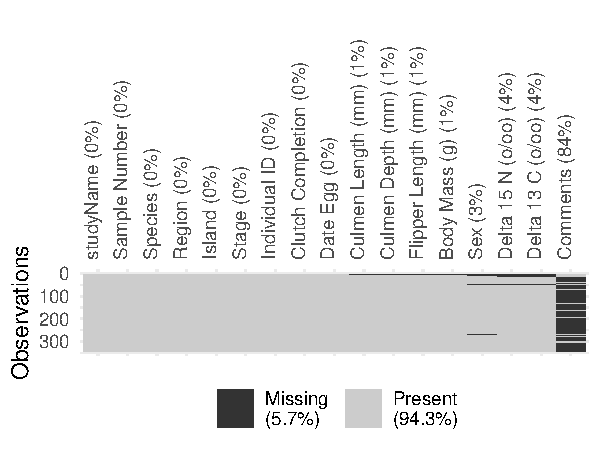
\includegraphics[width=\maxwidth]{figure/listings-par_mar_c_2_2_2_2__-1} 

}

\end{Schunk}
For simplicity we'll remove any observations (rows) that have missing values.
\begin{Schunk}
\begin{Sinput}
penguins_clean = tidyr::drop_na(penguins_clean, sex)
\end{Sinput}
\end{Schunk}
Compare the number of observations between the original and the clean data frame:
\begin{Schunk}
\begin{Sinput}
nrow(penguins)
\end{Sinput}
\begin{Soutput}
[1] 344
\end{Soutput}
\end{Schunk}
\begin{Schunk}
\begin{Sinput}
nrow(penguins_clean)
\end{Sinput}
\begin{Soutput}
[1] 333
\end{Soutput}
\end{Schunk}
We have made two changes to \lstinline|penguins_raw| to get to \lstinline|penguins_clean|. We can summarise this in an easy to read \textbf{pipeline}:
\begin{Schunk}
\begin{Sinput}
penguins_clean = penguins_raw |>
  janitor::clean_names() |>
  tidyr::drop_na(sex)
\end{Sinput}
\end{Schunk}
\subsubsection{Palmer penguins cross tabulation}
The \textbf{janitor} package has a range of functions that help with importing data and doing quick tabulations
\begin{Schunk}
\begin{Sinput}
library(janitor)
penguins_clean |>
  janitor::tabyl(species, sex) |>
  janitor::adorn_totals(where = c("row", "col"))
\end{Sinput}
\begin{Soutput}
                                   species FEMALE MALE Total
       Adelie Penguin (Pygoscelis adeliae)     73   73   146
 Chinstrap penguin (Pygoscelis antarctica)     34   34    68
         Gentoo penguin (Pygoscelis papua)     58   61   119
                                     Total    165  168   333
\end{Soutput}
\end{Schunk}
\subsubsection{Visualising the Palmer penguins data}
We'll use the \textbf{ggplot2} package extensively. There are three key components:
\begin{itemize}
  	\item input a data frame
	\item mapping aesthetics \lstinline|aes()| where you specify what goes on the axes, how to
	colour variables, what the groups are, etc.
	\item geometries \lstinline|geom_****()| that you add to build up the plot
\end{itemize}
\subsubsection{Mutating a variable}
The \lstinline|species| variable is a bit long. For visualisation purposes we only really need the first word of the species variable. The code below adds to the \textbf{pipeline} we saw earlier by creating a new variable, \lstinline|species_short|, that extracts the first word from the species variable.
\begin{Schunk}
\begin{Sinput}
penguins_clean = penguins_raw |>
  janitor::clean_names() |>
  tidyr::drop_na(sex) |>
  dplyr::mutate(
  species_short = stringr::word(species, start = 1, end = 1)
  )
penguins_clean |>
  dplyr::select(species, species_short) |>
  dplyr::distinct()
\end{Sinput}
\begin{Soutput}
# A tibble: 3 x 2
  species                                   species_short
  <chr>                                     <chr>        
1 Adelie Penguin (Pygoscelis adeliae)       Adelie       
2 Gentoo penguin (Pygoscelis papua)         Gentoo       
3 Chinstrap penguin (Pygoscelis antarctica) Chinstrap    
\end{Soutput}
\end{Schunk}
\begin{itemize}
	\item The \lstinline|ggplot()| function knows about the data frame \lstinline|penguins|.
	\item We add (\lstinline|+|) the bar chart geometry, \lstinline|geom_bar()|, to our blank canvas.
	\item Make the bars represent \textbf{proportions} within each species:
	\item Increase the font size and change the theme.
	\item Tidy up the axis labels.
	\item What if we want percent on the y-axis?
	\item Is it the same across all islands?
	\item Remove empty categories from the x axis.
\end{itemize}
\begin{Schunk}
\begin{Sinput}
ggplot(data = penguins_clean) + 
  aes(x = species_short, fill = sex) +
  geom_bar(position = "fill") +
  theme_linedraw() +
  scale_fill_manual(values=c("#992240", "#409922")) +
  labs(x = "", y = "Proportion of penguins", fill = "Sex") +
  scale_y_continuous(labels = scales::percent_format()) +
  facet_grid(cols = vars(island), scales = "free_x", space = "free_x")
\end{Sinput}


{\centering 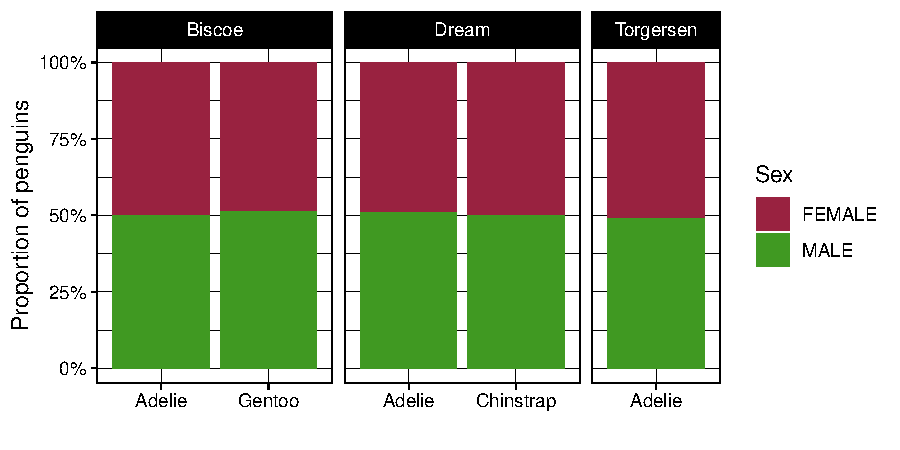
\includegraphics[width=\maxwidth]{figure/listings-unnamed-chunk-11-1} 

}

\end{Schunk}
\section{Collecting data}\label{sec:2}
\subsection{Sample surveys}
\subsubsection{Polling fail}
\begin{itemize}
    \item 1936 US Presidential election
    \item Franklin D. Roosevelt was completing his term of office
    \item America was struggling with high unemployment (16\%) following the Great Depression
    \item Literary Digest polled \textbf{10 million} people (mail survey)
    \item 24\% response rate (\textbf{2.4 million} people reply)
    \item They had correctly predicted the winner at every election since 1916
    \item Predicted victory for \textcolor{myred}{Landon}
\end{itemize}
\subsubsection{Gallup poll}
\begin{itemize}
    \item George Gallup was setting up his survey organisation.
    \item He drew 3000 people and predicted the Digest results.
    \item He also drew 50,000 people and correctly predicted Roosevelt victory. The actual prediction was off by a bit: 56\% predicted instead of 62\%
\end{itemize}
\begin{greenbox}
	\textbf{What went wrong?!?}
\end{greenbox}
\subsubsection{Why not observe the whole population?}
\begin{bluebox}{Typical limitations}
\begin{itemize}
    \item Hard to observe the population
    \item Not enough time
    \item Not enough money
    \item Not enough resources
\end{itemize}
\end{bluebox}
The solution is for us to draw samples and hope or expect to make general statement about the entire population.
\subsubsection{Sampling}
\begin{bluebox}{Definition}
    \textbf{Sampling} is the process of selecting a subset of representative observations from a population of interest so that characteristics from the subset (sample) can be used to draw conclusion or making inference about the entire population.
\end{bluebox}
Why sample?
\begin{itemize}
    \item Reduce the number of measurements
    \item Save time, money and resources
    \item Might be essential in destructive testing
\end{itemize}
\subsubsection{Sampling procedure}
\begin{itemize}
    \item What sample size is needed for my study?
    \item How the design will affect the sample size?
    \item Appropriate \textbf{survey design} provides the best estimation with high reliability at the lowest cost with the available resources.
    \begin{itemize}
        \item What survey design is appropriate for my study?
        \item How survey will be conducted/implemented?            
    \end{itemize}
\end{itemize}
\subsubsection{Types of biases}
\begin{itemize}
    \item Selection bias
    \item Recall bias
    \item Sensitive questions
    \item Misinterpret the questions
    \item Wording of question
    \item Other attributes of the interview as a source of bias…
\end{itemize}
\subsubsection{Getting an opinion}
\begin{greenbox}
	\textbf{Phrasing 1}\\
	Should a woman have control over her own body, including her reproductive system?
\end{greenbox}
\begin{greenbox}
	\textbf{Phrasing 2}\\
	Should a doctor be allowed to murder unborn children who can't defend themselves?
\end{greenbox}
\subsubsection{Measurement bias}
Schuman \& Converse (1971) performed a study to check whether or not the race of the interviewer inuenced responses after major racial riots in 1968 in Detroit. A sample of 395 African American were asked:
\begin{tcolorbox}[bluestyleline]
	\blockquote{Do you personally feel that you can trust most white people, some white people, or none at all}
\end{tcolorbox}
\begin{itemize}
    \item White interviewer: 35\% responded ``most'' \( (n=165) \)
    \item African American interviewer: 7\% responded ``most'' \( (n=330) \)
\end{itemize}
\subsubsection{Back to the 1936 US election}
\begin{itemize}
	\item The 2.4 million responses didn't even represent the 10 million people who were sent the surveys let alone the general voting population.
	\item Non-response bias: the people who didn't respond were different to those that did respond.
	\item Selection bias: addresses sourced from car registration and phone books (skewed towards wealthy Americans).
\end{itemize}
\begin{goldbox}
	When a selection procedure is biased, taking a larger sample DOES NOT help. This just repeats the basic mistake at a larger scale.
\end{goldbox}
\subsubsection{Bias}
\begin{bluebox}{Definition}
	Bias is any factor that favours certain outcomes or responses, or inuences an individual's responses. Bias may be unintentional (accidental), or intentional (to achieve certain results).
\end{bluebox}
When looking at data from a survey think about:
\begin{itemize}
	\item \textbf{Selection bias / sampling bias:} the sample does not accurately represent the population. Example: Attendees at a Star Trek convention may report that their favorite genre is science fiction
	\item \textbf{Non-response bias:} Certain groups are under-represented because they elect not to participate. Example: a restaurant may give each table a ``customer satisfaction'' survey with their bill.
	\item \textbf{Measurement or designed bias:} Bias factors in the sampling method influence the data obtained. Example: a respondent may answer questions in the way she thinks the questioner wants her to answer.		
\end{itemize}
\subsection{Controlled experiments}
\subsubsection{Randomised controlled double-blind trials}
\begin{greenbox}
	\textbf{What is a randomised controlled double-blind study? Why is it good but rare?}
\end{greenbox}
\begin{enumerate}
	\item Investigators obtain a representative sample of subjects.
	\item Investigators randomly allocate the subjects into a \textbf{\textcolor{mygreen}{treatment}} group and a \textbf{\textcolor{myred}{control}} group.
	\item The \textbf{\textcolor{myred}{control group}} is given a placebo, but neither the subjects nor the investigators know the identity of the 2 groups (double-blind).
	\item Investigators compare the responses of the 2 groups.
	\item The design is good because we expect the 2 groups to be similar, hence any difference in the responses is likely to be caused by the treatment
\end{enumerate}
\subsection{Observational studies}
\subsubsection{Does smoking cause cancer?}
\begin{tcolorbox}[bluestyleline]
	\blockquote{Tobacco smoking is the largest preventable cause of cancer, responsible for more cancer deaths in Australia than any other single factor. It is also directly responsible for many heart and lung diseases.}
	-- Australian Cancer Council
\end{tcolorbox}
\begin{tcolorbox}[bluestyleline]
	\blockquote{In a hearing to the Australian High Court in 2012 disputing the introduction of cigarette plain packaging with health warnings, while British American Tobacco was prepared to accept that there are serious health consequences caused by smoking, Imperial Tobacco responded \textbf{some people say that\dots}}
	-- The Sydney Morning Herald
\end{tcolorbox}
\subsubsection{The need for observational studies}
\begin{itemize}
	\item By necessity, many research questions require an \textbf{observational study}, rather than a controlled experiment.
	\item For example, with a study on the effects of smoking, investigators cannot choose which subjects will be in the \textbf{\textcolor{mygreen}{treatment group}} (smoking). Rather, they must \textbf{observe} medical results for the 2 groups.
	\item Smilarly, most \textbf{educational research} is based on observational studies.
	\item The conclusions of observational studies require great care.
\end{itemize}
\begin{goldbox}
	\textbf{Observational studies can not establish causation.}
\end{goldbox}
\begin{itemize}
\item A good \textbf{randomised controlled experiment} can establish causation, an \textbf{observational study} can only establish association.
\item An observational study may \textit{suggest} causation, but it can't \textit{prove} causation.
\end{itemize}
\subsubsection{Misleading hidden confounders}
\begin{itemize}
	\item Confounding occurs when the \textbf{\textcolor{mygreen}{treatment group}} and \textbf{\textcolor{myred}{control group}} differ by some third variable (other than the treatment) which influences the response that is studied.
	\item Confounders can be hard to find, and can mislead about a cause and effect relationship.
	\item Confounding (or lurking) variables can be introduced into a randomised study if any of the subjects drop out, causing \textbf{selection bias} or \textbf{survivor bias}. Similarly, if not all subjects keep taking the treatment or placebo, we get the confounding of \textbf{adherers} and \textbf{non-adherers}.
\end{itemize}
\subsubsection{Lung cancer associations}
\begin{greenbox}
	\textbf{A study finds that having yellow fingertips is associated with lung cancer. Does having yellow fingertips cause lung cancer?}
\end{greenbox}
\begin{greenbox}
	\textbf{A study finds that smokers tend to have higher rates of lung cancer. Does smoking cause lung cancer?}
\end{greenbox}
\subsubsection{Strategy for dealing with confounders}
Sometimes we can make the groups more comparable by dividing them into subgroups with respect to the confounder.
For example, if alcohol consumption is a potential confounding factor for smoking's affect on liver cancer, we can divide our subjects into 3 groups:
\begin{itemize}
	\item heavy drinkers
	\item medium drinkers
	\item light drinkers
\end{itemize}
This is called \textbf{controlling} for alcohol consumption.
\subsubsection{Controlling for confounding}
We can control for confound by making 3 separate comparisons:
\begin{itemize}
	\item heavy drinking: smokers vs non-smokers
	\item medium drinking: smokers vs non-smokers
	\item light drinking: smokers vs non-smokers
\end{itemize}
\begin{greenbox}
	\textbf{What are the limitations of this strategy?}
\end{greenbox}
\subsubsection{Is smoking good for your longevity?}
A famous study by Appleton et al. (1996) considered data on female subjects 20 years apart. Two studies:
\begin{itemize}
	\item initial data from a 1 in 6 survey from an electoral roll in a mixed urban and rural area near Newcastle upon Tyne UK Tunbridge et al. (1977).
	\item follow-up data 20 years later Vanderpump et al. (1995).
\end{itemize}
The study concentrated on the 1314 women who were either smokers or non- smokers (in the full data, only 162 had stopped smoking and only 18 did not record their status).
\begin{Schunk}
\begin{Sinput}
x = read_csv("https://git.io/fNGXk")
x
\end{Sinput}
\begin{Soutput}
# A tibble: 4 x 3
  status     survival count
  <chr>      <chr>    <dbl>
1 Smoker     Died       139
2 Smoker     Survived   443
3 Non-smoker Died       230
4 Non-smoker Survived   502
\end{Soutput}
\begin{Sinput}
x_long = tidyr::uncount(x, weights = count)
dim(x_long)
\end{Sinput}
\begin{Soutput}
[1] 1314    2
\end{Soutput}
\begin{Sinput}
x_long |> 
  dplyr::group_by(status) |>
  dplyr::summarise(
		 rate = sum(survival == "Died")/n()
	)
\end{Sinput}
\begin{Soutput}
# A tibble: 2 x 2
  status      rate
  <chr>      <dbl>
1 Non-smoker 0.314
2 Smoker     0.239
\end{Soutput}
\begin{Sinput}
x_long |>
  dplyr::summarise(
  		 rate = sum(survival == "Died")/n()
  )
\end{Sinput}
\begin{Soutput}
# A tibble: 1 x 1
   rate
  <dbl>
1 0.281
\end{Soutput}
\begin{Sinput}
ggplot(x) +
  aes(x = status,
  y = count,
  fill = survival) +
  geom_bar(stat = "identity",
  position = "fill") +
  scale_y_continuous(
  labels = scales::percent_format()) +
  labs(x = "", y = "Proportion") +
  theme_minimal() +
  scale_fill_manual(values=c("#992240", "#409922"))
\end{Sinput}


{\centering 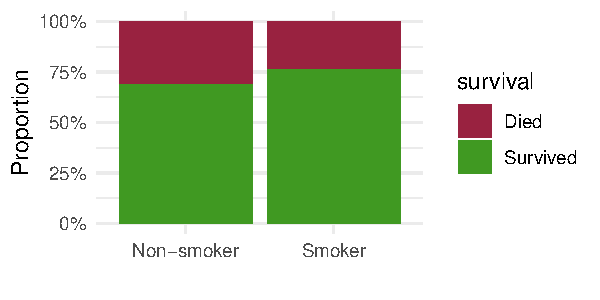
\includegraphics[width=\maxwidth]{figure/listings-unnamed-chunk-12-1} 

}

\end{Schunk}
\subsection{Simpson's Paradox}
\subsubsection{What is Simpson's Paradox?}
\begin{itemize}
	\item Simpson's Paradox was first mentioned by British statistician Udny Yule in 1903.
	\item It is named after Edward H. Simpson (Simpson, 1951)
	\item Sometimes there is a clear trend in individual groups of data that disappears when the groups are pooled together.
	\item It occurs when relationship between percentages in subgroups are reversed when the subgroups are combined, because of a confounding or lurking variable.
	\item The association between a pair of variables \( (X,Y) \) reverses sign upon conditioning of a third variable \( Z \), regardless of the value taken by \( Z \).
\end{itemize}
\begin{goldbox}
	Observational studies with a confounding variable can lead to \textbf{Simpson's paradox}
\end{goldbox}
\subsubsection{Mortality by Age Group}
\begin{Schunk}
\begin{Sinput}
y = readr::read_csv("https://git.io/fNGSi")
dplyr::glimpse(y, width = 80)
\end{Sinput}
\begin{Soutput}
Rows: 28
Columns: 4
$ status    <chr> "Smoker", "Smoker", "Smoker", "Smoker", "Smoker", "Smoker", ~
$ survival  <chr> "Died", "Died", "Died", "Died", "Died", "Died", "Died", "Sur~
$ age_group <chr> "18-24", "25-34", "35-44", "45-54", "55-64", "65-74", "75+",~
$ count     <dbl> 2, 3, 14, 27, 51, 29, 13, 53, 121, 95, 103, 64, 7, 0, 1, 5, ~
\end{Soutput}
\begin{Sinput}
ytab = y |>
  tidyr::pivot_wider(id_cols = age_group, 
                     names_from = c(status, survival), 
                     values_from = count,
                     names_sep = ": ")
ytab |> 
  knitr::kable(booktabs = TRUE) |>
  kable_styling(position="center", latex_options = "hold_position")
\end{Sinput}
\begin{table}[!h]
\centering
\begin{tabular}{lrrrr}
\toprule
age\_group & Smoker: Died & Smoker: Survived & Non-smoker: Died & Non-smoker: Survived\\
\midrule
18-24 & 2 & 53 & 1 & 61\\
25-34 & 3 & 121 & 5 & 152\\
35-44 & 14 & 95 & 7 & 114\\
45-54 & 27 & 103 & 12 & 66\\
55-64 & 51 & 64 & 40 & 81\\
\addlinespace
65-74 & 29 & 7 & 101 & 28\\
75+ & 13 & 0 & 64 & 0\\
\bottomrule
\end{tabular}
\end{table}

\begin{Sinput}
mortality = y |> 
  uncount(weights = count) |> 
  group_by(status, age_group) |> 
  summarise(rate = mean(survival=="Died"))
mortality |> 
  ggplot() + 
  aes(x = age_group, y = rate, fill = status) +
  geom_bar(stat = "identity", position = "dodge") +
  theme_minimal() +
  scale_fill_manual(values=c("#992240", "#409922")) +
  scale_y_continuous(labels = scales::percent_format()) + 
  labs(title = "Mortality rates by age group",
  	   y = "Mortality rate", 
  	   x = "Age group",
  fill = "") +
  theme(panel.grid.major.y = element_blank()) +
  coord_flip()
\end{Sinput}


{\centering 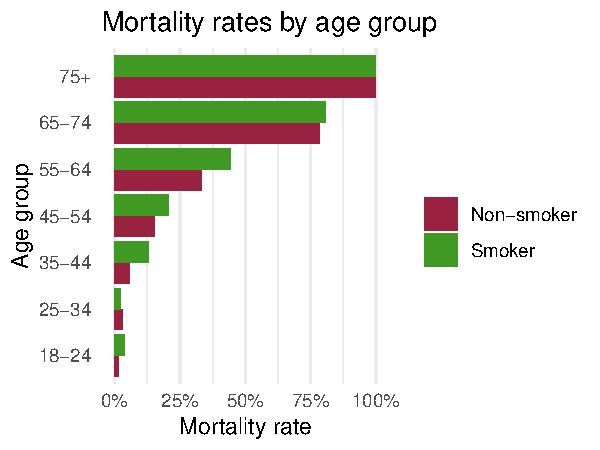
\includegraphics[width=\maxwidth]{figure/listings-unnamed-chunk-13-1} 

}

\end{Schunk}
\begin{itemize}
	\item Not many young people died.
	\item Most old people died.
	\item In the middle age groups, smokers tended to have higher mortality rates than non-smokers
\end{itemize}
\subsubsection{How did we got the wrong overall conclusion?}
Consider the distribution of samples by smoking status across age groups.
\begin{Schunk}
\begin{Sinput}
# convert into "long" form
mortality_long = y |> uncount(weights = count)
mortality_long |>
  ggplot() +
  aes(x = age_group, fill = status) +
  geom_bar() +
  theme_minimal() +
  scale_fill_manual(values=c("#992240", "#409922")) +
  labs(y = "Count",
  	   x = "Age group",
  fill = "") +
  theme(panel.grid.major.y = element_blank(),) +
  guides(fill = guide_legend(reverse = TRUE)) +
  coord_flip()
\end{Sinput}


{\centering 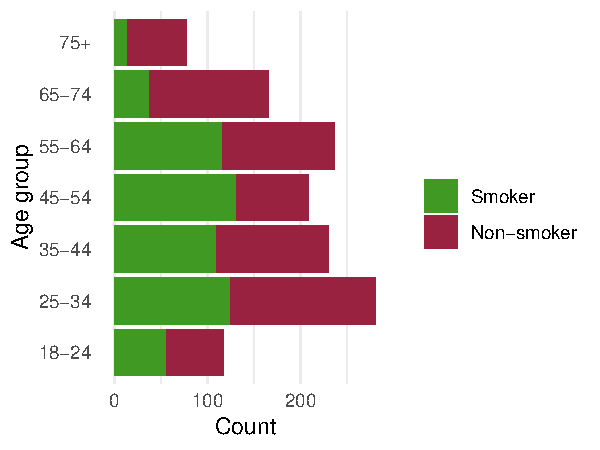
\includegraphics[width=\maxwidth]{figure/listings-unnamed-chunk-14-1} 

}

\end{Schunk}
\begin{itemize}
	\item As there are many more young women who smoked than older women, and as younger women are expected to live longer than older women, adding all the groups together makes smoking appear to be beneficial.
	\item This is a classic example of \textbf{Simpson's paradox}: a trend present within multiple groups can reverse when the groups are combined.
\end{itemize}
\section{Chi-squared tests}\label{sec:3}
\subsection{Genetic linkage}
In a backcross experiment to investigate the \textbf{genetic linkage} between two genes \( A \) and \( B \) in a species of flower. Researchers classified 400 offspring by phenotype:
\begin{table}[h]
	\centering
	\begin{tabular}{@{}lllll@{}}
	\textbf{Phenotype} & \( AB \) & \( ab \) & \( aB \) & \( ab \) \\ \midrule
	Count              & 128 & 86 & 74 & 112 \\ 
	\end{tabular}
\end{table}
\begin{itemize}
	\item \( A \) might be pink flowers and \( a \) might be yellow flowers
	\item \( B \) might be smooth leaves and \( b \) might be wrinkled leaves
	\begin{itemize}
		\item \( AB \) means a plant with pink flowers and smooth leaves
		\item \( ab \) means a plant with pink flowers and wrinkled leaves
		\item \( aB \) means a plant with yellow flowers and smooth leaves
		\item \( ab \) means a plant with yellow flowers and wrinkled leaves
	\end{itemize}
\end{itemize}
Under the \textit{no linkage} model, the four phenotypes are equally likely. So we would expect to see equal proportions for each phenotype:
\begin{table}[H]
	\centering
	\begin{tabular}{@{}lllll@{}}
	\textbf{Phenotype} 	& \( AB \) & \( ab \) & \( aB \) & \( ab \) \\ \midrule
	Expected proportion	& 0.25 & 0.25 & 0.25 & 0.25 \\ 
	\end{tabular}
\end{table}
If linkage is in the \textit{coupling phase}, the probabilities of the four phenotypes are given by
\begin{table}[H]
	\centering
	\begin{tabular}{@{}lllll@{}}
	\textbf{Phenotype} 	& \( AB \) & \( ab \) & \( aB \) & \( ab \) \\ \midrule
	Expected proportion & \( \frac{1}{2}(1-p) \) & \( \frac{1}{2}p \) & \( \frac{1}{2}p \) & \( \frac{1}{2}(1-p) \) \\ 
	\end{tabular}
\end{table}
where \( p \) is the \textbf{\textcolor{mygreen}{recombination fraction}}. We will need to estimate \( p \) as the overall proportion of observed \( Ab \) and \( aB \)
\subsection{No linkage model}
\subsubsection{No linkage model}
\begin{itemize}
	\item \textbf{Null hypothesis}: each of the phenotypes are equally likely.
	\item \textbf{Alternative hypothesis}: the phenotypes are not equally likely.
\end{itemize}
Let \( p_i \) be the probability of being in the \( i \)th phenotype \( i = AB,Ab,aB,ab \).\\
Under the null hypothesis (i.e. assuming that the no linkage model is correct) the counts are uniformly distributed across the 4 categories,
\[
	p_i = 0.25 \;\text{for all}\; i
\]
\begin{Schunk}
\begin{Sinput}
# observed counts
y = c(128, 86, 74, 112) 
n = sum(y)
# hypothesised proportions
p = c(1/4, 1/4, 1/4, 1/4) 
# expected counts
e = p*n
names = c("AB", "Ab", "aB", "ab")
df = tibble(
  phenotype = names,
  # observed counts
  y = y,
  # hypothesised proportions
  p = p,
  # expected counts
  e = n * p
)
df
\end{Sinput}
\begin{Soutput}
# A tibble: 4 x 4
  phenotype     y     p     e
  <chr>     <dbl> <dbl> <dbl>
1 AB          128  0.25   100
2 Ab           86  0.25   100
3 aB           74  0.25   100
4 ab          112  0.25   100
\end{Soutput}
\begin{Sinput}
df |> ggplot() +
  aes(x = phenotype, y = y) +
  geom_col(alpha = 0.6) +
  geom_hline(yintercept = 100,
  colour = "#224099",
  linewidth = 2) +
  labs(x = "", y = "Count") + 
  theme_classic()
\end{Sinput}


{\centering 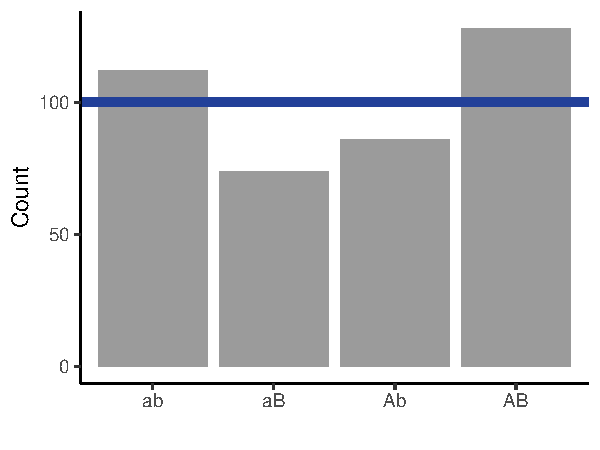
\includegraphics[width=\maxwidth]{figure/listings-unnamed-chunk-15-1} 

}

\end{Schunk}
Differences between observed counts and expected counts:
\begin{Schunk}
\begin{Sinput}
df = df |>
  mutate(d = y - e)
df
\end{Sinput}
\begin{Soutput}
# A tibble: 4 x 5
  phenotype     y     p     e     d
  <chr>     <dbl> <dbl> <dbl> <dbl>
1 AB          128  0.25   100    28
2 Ab           86  0.25   100   -14
3 aB           74  0.25   100   -26
4 ab          112  0.25   100    12
\end{Soutput}
\begin{Sinput}
df |>
	summarise(avg_diff = mean(d))
\end{Sinput}
\begin{Soutput}
# A tibble: 1 x 1
  avg_diff
     <dbl>
1        0
\end{Soutput}
\end{Schunk}
\subsubsection{Test statistic}
The average of the differences doesn't tell us much. Let's take the squared differences, and ``normalise'' by dividing by the expected cell counts:
\[
	t_0 = \sum_{i=1}^{k} \frac{(y_i - e_i)^2}{e_i}
\]
where \( k \) is the number of categories (groups).
\begin{Schunk}
\begin{Sinput}
df = df |> mutate(
  squared_discrepency = (y-e)^2,
  contribution = (y-e)^2/e
  )
t0 = sum(df$contribution)
t0
\end{Sinput}
\begin{Soutput}
[1] 18
\end{Soutput}
\end{Schunk}
\subsubsection{Simulate}
Under the null hypothesis, the counts are uniformly distributed across the 4 categories.\\
Fixing the sample size at \( n = 400 \) we can \textbf{simulate} data assuming the null hypothesis is true.
\begin{Schunk}
\begin{Sinput}
n = 400
set.seed(88)
sim1 = sample(
  x = names,
  size = n,
  replace = TRUE,
  prob = c(0.25,0.25,0.25,0.25)
)
table(sim1)
\end{Sinput}
\begin{Soutput}
sim1
 ab  aB  Ab  AB 
103  89 105 103 
\end{Soutput}
\begin{Sinput}
barplot(table(sim1), main = "Simulated counts")
\end{Sinput}


{\centering 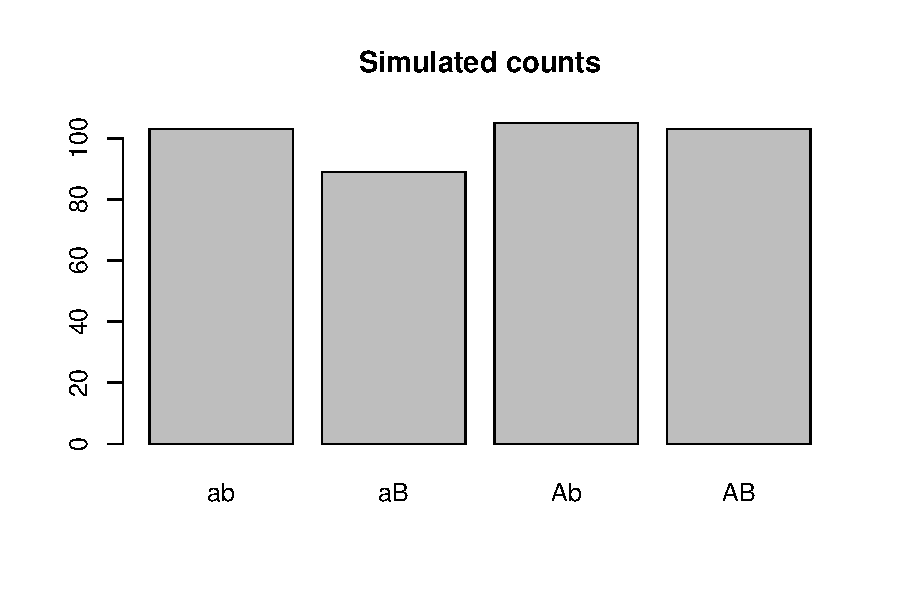
\includegraphics[width=\maxwidth]{figure/listings-unnamed-chunk-18-1} 

}

\end{Schunk}
Our test statistic for that simulated sample is:
\begin{Schunk}
\begin{Sinput}
sim_y = table(sim1)
sum((sim_y - e)^2/e)
\end{Sinput}
\begin{Soutput}
[1] 1.64
\end{Soutput}
\end{Schunk}
which is alot smaller than what we observed on our \textbf{actual data}:
\begin{Schunk}
\begin{Sinput}
t0
\end{Sinput}
\begin{Soutput}
[1] 18
\end{Soutput}
\end{Schunk}
\begin{Schunk}
\begin{Sinput}
B = 3000
sim_t_stats = vector(mode = "numeric", length = B)
for(i in 1:B){
  sim = sample(x = names, size = n,
  replace = TRUE, prob = c(0.25,0.25,0.25,0.25))
  sim_y = table(sim)
  sim_t_stats[i] = sum((sim_y - e)^2/e)
}
hist(sim_t_stats, main = "", breaks = 20)
\end{Sinput}


{\centering 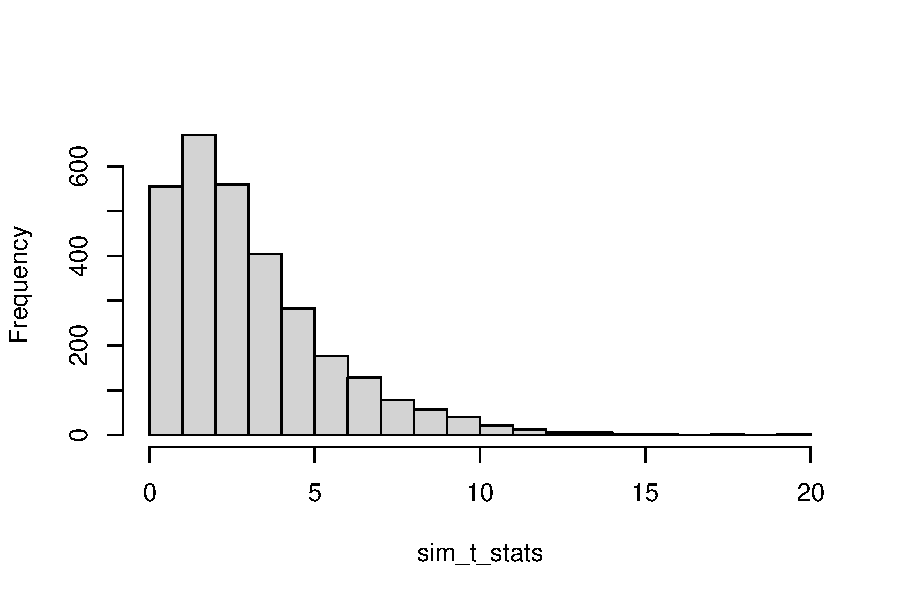
\includegraphics[width=\maxwidth]{figure/listings-unnamed-chunk-21-1} 

}

\end{Schunk}
\begin{itemize}
	\item Now we have a pretty good idea about the shape of the \textbf{distribution} of the test statistic \textcolor{mygreen}{when the null hypothesis is true}.
	\item We can compare the test statistic that we calculated on the original data to the \textcolor{mygreen}{``null distribution''}
	\item One way to do this is to ask the question:
\end{itemize}
\begin{quote}
	Given that the \textcolor{mygreen}{null hypothesis is true}, how likely is it that we observe a test statistic as or more extreme than that we calculated from our original sample?
\end{quote}
\begin{Schunk}
\begin{Sinput}
# sum(sim_t_stats >= t0)/B
mean(sim_t_stats >= t0)
\end{Sinput}
\begin{Soutput}
[1] 0.0003333333
\end{Soutput}
\end{Schunk}
In 0.1\% of samples when the null hypothesis is true, we got a simulated sample that was ``more extreme'' than our original sample.
\subsubsection{Is there way to do it without simulation?}
Yes! A \( \chi^2 \) test!\\
In this example the test statistic,
\[
	T = \sum_{i=1}^{k} \frac{(Y_i - e_i)^2}{e_i} \sim \chi^2_{k-1},
\]
approximately, where \( k \) is the number of groups.\\
Let's compare this distribution to the simulated test statistic distribution.
\begin{Schunk}
\begin{Sinput}
hist(sim_t_stats, main = "", breaks = 20, probability = TRUE, ylim = c(0, 0.25))
curve(dchisq(x, df = 3), add = TRUE, col = "#224099", lwd = 2)
\end{Sinput}


{\centering 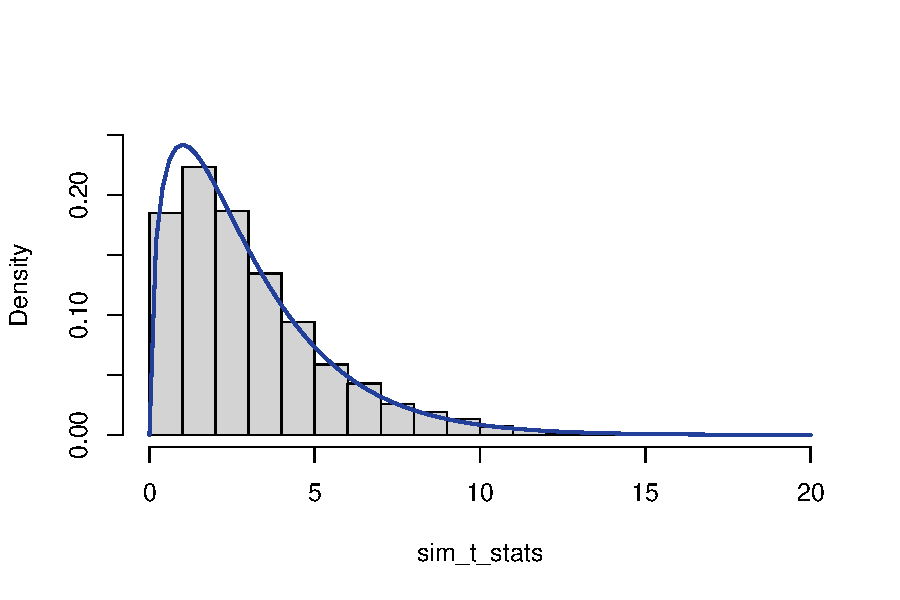
\includegraphics[width=\maxwidth]{figure/listings-unnamed-chunk-23-1} 

}

\end{Schunk}
\subsubsection{\( \chi^2 \) test degrees of freedom}
\begin{itemize}
	\item The \textbf{degrees of freedom} is \( k-1 \) because the first \( k-1 \) observations \( y_i \) contain all the information and the last observation is fixed by \( y_k = n - \sum\limits_{i=1}^{k-1} y_i \) adding no extra information.
	\item In general, the test statistic takes the form,
	\[
		T = \sum_{i=1}^{k} \frac{(Y_{i-e_i})^2}{e_i} \sim \chi^2_{k-1-q}
	\]
	where \( q \) is the number of parameters that need to be estimated from the sample.
	\item In the no linkage example, \( q = 0 \) because we do not need to estimate any parameters (i.e. we don't need to estimate the hypothesised proportions, all \( p_{i0} = 0.25 \)).
	\item  The approximation will only be accurate if \textit{no expected frequency} is too small, as a rule of thumb we require all \( e_i \geq 5 \). Otherwise, we need to pool adjacent categories so that the expected frequencies are always \( \geq 5 \).
\end{itemize}
\begin{redbox}{Workflow: Chi-squared goodness of fit test}
	One categorical variable from a single population and want to see if it follows a hypothesised distribution.
	\begin{itemize}
		\item \textbf{Hypothesis}: \( H_0 \): the proportions in each category \( (p_i) \) are equal to the corresponding hypothesised proportions \( (p_{i0}) \), i.e. \( p_1 = p_{10}, p_2 = p_{20}, \dotsc, p_k = p_{k0} \) vs \( H_1 \): at least proportion is not equal to the hypothesised proportion, i.e. at least one equality does not hold.
		\item \textbf{Assumptions}: independent observations and \( e_i = np_{i0} \geq 5 \)
		\item \textbf{Test statistic}: \( T = \sum\limits_{i=1}^{k} \frac{(Y_i -e_i)^2}{e_i} \). Under \( H_0, T \sim \chi^2_{k-1-q} \) approximately, where \( k \) is the number of groups and \( q \) is the number of parameters that needs to be estimated from the data.
		\item \textbf{Observed test statistic}: \( \sum\limits_{i=1}^{k} \frac{(Y_{i-e_i})^2}{e_i} \).
		\item \textbf{P-value}: \( P(T\geq t_0) = P(\chi^2_{k-1-q} \geq t_0) \)
		\item \textbf{Decision}: Reject \( H_0 \) if the p-value \( < \alpha \), otherwise do not reject \( H_0 \).
	\end{itemize}
\end{redbox}
\subsubsection{Table for calculating the test statistic}
The calculations can be summarised in the following table:
\begin{table}[H]
	\centering
	\begin{tabular}{@{}c|ccccc@{}}
	Group \( i \) & \( y_i \)  	 & \( p_{i0} \) & \( e_i = np_{i0} \) & \( y_i - e_i \) & \( \frac{(y_i - e_i)^2}{e_i} \) \\ \midrule
	\( 1 \) 	  & \( y_1 \)  	 & \( p_{10} \) & \( np_{10} \)       & \( y_1 - e_1 \) & \( (y_1 - e_1)^2/e_1 \) \\
	\( 2 \)   	  & \( y_2 \)  	 & \( p_{20} \) & \( np_{20} \)	  	  & \( y_2 - e_2 \) & \( (y_2 - e_2)^2/e_2 \) \\
	\( \vdots \)  & \( \vdots \) & \( \vdots \) & \( \vdots \) 	  	  & \( \vdots \) 	& \( \vdots \) 					  \\
	\( k \)   	  & \( y_k \) 	 & \( p_{k0} \)	& \( np_{k0} \) 	  & \( y_k - e_k \) & \( (y_k - e_k)^2/e_k \) \\ \midrule
	Sum 		  & \( n \) 	 & 1 			& \( n \) 			  & 0 				& \( t_0 \) 
	\end{tabular}
\end{table}
\begin{itemize}
	\item \( y_i \) are the observed counts
	\item \( p_{i0} \) are the hypothesised probabilities
	\item \( e_i \) are the expected counts \textit{assuming the null hypothesis is true}
	\item \( t_0 \) is the observed test statistic
\end{itemize}
\subsubsection{No linkage model}
Under the \textit{no linkage model} we assume that the observations are uniformly distributed across the four categories, i.e. the hypothesised probabilities are \( p_{i0} = \frac{1}{4} \) for \( i = 1,2,3,4 \):
\begin{itemize}
	\item \textbf{Hypothesis}: The null hypothesis is a no linkage model with uniform probabilities,\( H_0 : p_{AB} = p_{Ab} = p_{aB} = p_{ab} = \frac{1}{4} \). The alternative is anything other than a no linkage model, \( H_1 \): at least one equality does not hold.
	\item \textbf{Assumptions}: independent observations and expected cell counts at least 5, \( e_i = np_{i0} \geq 5 \)
	\item \textbf{Test statistic}: \( T = \sum\limits_{i=1}^{k} \frac{(Y_i - e_i)^2}{e_i} \). Under \( H_0, T \sim \chi^2_3 \) approximately.
	\item \textbf{Observed test statistic}: \( t_0 = 18 \).
	\item \textbf{P-value}: \( P(T\geq t_0) = P(\chi^2_3 \geq 18) =  0.0004 \)
	\item \textbf{Decision}: Since the p-value is much smaller than 0.05, there is strong evidence in the data against \( H_0 \). Hence the four phenotypes are not equally likely and we reject the no linkage model.
\end{itemize}
\begin{table}[H]
	\centering
	\begin{tabular}{@{}cc|cccc@{}}
	Type 	 & \( i \) & \( y_i \) & \( e_i = np_{i0} \) 				& \( y_i - e_i \)      & \( \frac{(y_i - e_i)^2}{e_i} \) \\ \midrule
	\( AB \) & 1 	   & 128  	   & \( 400 \times \frac{1}{4} = 100 \)	& \( 128 - 100 = 28 \) & \( \frac{(28)^2}{100} = 7.84 \)   \\
	\( Ab \) & 2   	   & 86  	   & \( 400 \times \frac{1}{4} = 100 \) & \( 86 - 100 = -14 \) & \( \frac{(-14)^2}{100} = 1.96 \)   \\
	\( aB \) & 3 	   & 74 	   & \( 400 \times \frac{1}{4} = 100 \) & \( 74 - 100 = -26 \) & \( \frac{(-26)^2}{100} = 6.76 \)	 \\
	\( ab \) & 4   	   & 112 	   & \( 400 \times \frac{1}{4} = 100 \) & \( 112 - 100 = 12 \) & \( \frac{(12)^2}{100} = 1.44  \)  \\ \midrule
	Total 	 & 	 	   & 400	   & \( 400 \times \frac{1}{4} = 100 \)	& 0 				   & \( t_0 = 18.00 \) 
	\end{tabular}
\end{table}
\begin{Schunk}
\begin{Sinput}
1 - pchisq(18, df = 3)
\end{Sinput}
\begin{Soutput}
[1] 0.0004398497
\end{Soutput}
\begin{Sinput}
(ey=n*p) # expected counts
\end{Sinput}
\begin{Soutput}
[1] 100 100 100 100
\end{Soutput}
\begin{Sinput}
ey>=5 # test e_i >= 5
\end{Sinput}
\begin{Soutput}
[1] TRUE TRUE TRUE TRUE
\end{Soutput}
\end{Schunk}
The \lstinline|chisq.test()| function in R can do it all for us. We give it the vector of observed counts and the vector of hypothesised probabilities:
\begin{Schunk}
\begin{Sinput}
chisq.test(y, p = p)
\end{Sinput}
\begin{Soutput}

	Chi-squared test for given probabilities

data:  y
X-squared = 18, df = 3, p-value = 0.0004398
\end{Soutput}
\end{Schunk}
\subsection{Linkage model}
Under the \textit{coupling phase} linkage model, the probabilities of each of the four phenotype outcomes are given by
\begin{table}[H]
	\centering
	\begin{tabular}{@{}lllll@{}}
	\textbf{Phenotype} 	& \( AB \)				 & \( ab \) 		  & \( aB \) 		   & \( ab \) 				\\ \midrule
	Observed count		& 128					 & 86				  & 74		 		   & 112					\\ \midrule
	Expected proportion & \( \frac{1}{2}(1-p) \) & \( \frac{1}{2}p \) & \( \frac{1}{2}p \) & \( \frac{1}{2}(1-p) \) \\ 
	\end{tabular}
\end{table}
To test the linkage model hypothesis, we need to estimate the parameter \( p \), the recombination fraction from the observed data: \( \hat{p} \) is the proportion of observed offspring with phenotype \( Ab \) or \( aB \),
\[
	\hat{p} = \frac{86 + 74}{400} = 0.4
\]
Hence the four (estimated) hypothesised probabilities are,
\begin{Schunk}
\begin{Sinput}
y = c(128, 86, 74, 112)
p = c(0.3, 0.2, 0.2, 0.3)
names = c("AB", "Ab", "aB", "ab")
par(mfrow = c(1, 2)) # set up a graphics device with 1 row and 2 columns
barplot(y, names.arg = names, main = 'Observed frequencies')
barplot(p * sum(y), names.arg = names, main = 'Expected frequencies')
\end{Sinput}


{\centering 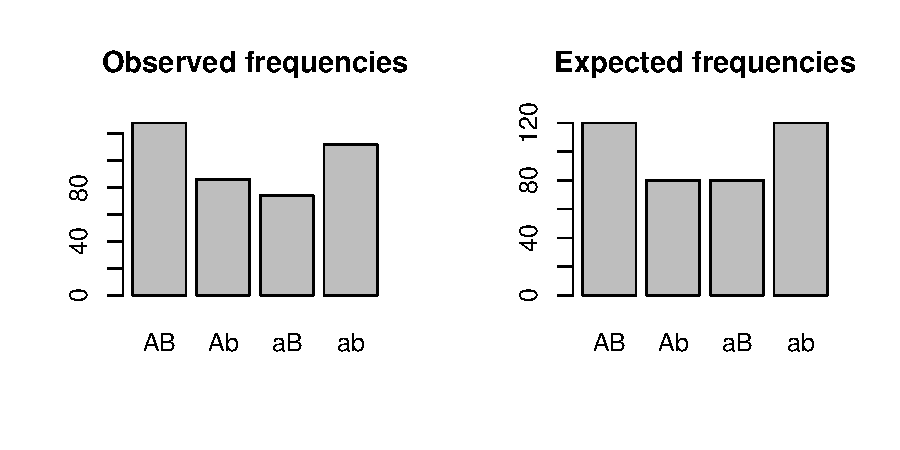
\includegraphics[width=\maxwidth]{figure/listings-unnamed-chunk-26-1} 

}

\end{Schunk}
\subsubsection{Test statistic}
The form of the observed test statistic is the same as in the no linkage model,
\[
	t_0 = \sum_{i=1}^{4} \frac{(y_i - e_i)^2}{e_i}
\]
but now the \( e_i \) are now calculated using the new hypothesised proportions.
\begin{table}[H]
	\centering
	\begin{tabular}{@{}ccrrr@{}}
	Type 	 & \( y_i \) & \( e_i = np_{i0} \) 				  & \( y_i - e_i \)      & \( \frac{(y_i - e_i)^2}{e_i} \)  \\ \midrule
	\( AB \) & 128  	 & \( 400 \times \frac{3}{4} = 120 \) & \( 128 - 120 = 8 \)  & \( \frac{(8)^2}{120} = 7.84 \)   \\
	\( Ab \) & 86  	     & \( 400 \times \frac{2}{4} = 80  \) & \( 86 - 80 = 6 \) 	 & \( \frac{(6)^2}{80} = 1.96 \)    \\
	\( aB \) & 74 	     & \( 400 \times \frac{2}{4} = 80  \) & \( 74 - 80 = -6 \) 	 & \( \frac{(-6)^2}{80} = 6.76 \)   \\
	\( ab \) & 112 	     & \( 400 \times \frac{3}{4} = 120 \) & \( 112 - 120 = -8 \) & \( \frac{(-8)^2}{120} = 1.44  \) \\ \midrule
	Total 	 & 400	     & 400	  				  		  	  & 0					 & \( t_0 = 1.96 \) 
	\end{tabular}
\end{table}
\subsubsection{Simulated null distribution}
\begin{Schunk}
\begin{Sinput}
n = 400
hyp_probs = c(0.3, 0.2, 0.2, 0.3)
B = 3000
sim_test_stats = vector(mode = "numeric", length = B)
for(i in 1:B){
  sim = sample(x = names, size = n, replace = TRUE, prob = hyp_probs)
  sim_y = table(sim)
  # estimated probability
  p_e = sum(table(sim)[2:3])/n
  # expected values using estimated probabilities
  e = 400*c(1 - p_e, p_e, p_e, 1 - p_e)/2
  sim_test_stats[i] = sum((sim_y - e)^2/e)
}
hist(sim_test_stats, main = "", breaks = 20)
\end{Sinput}


{\centering 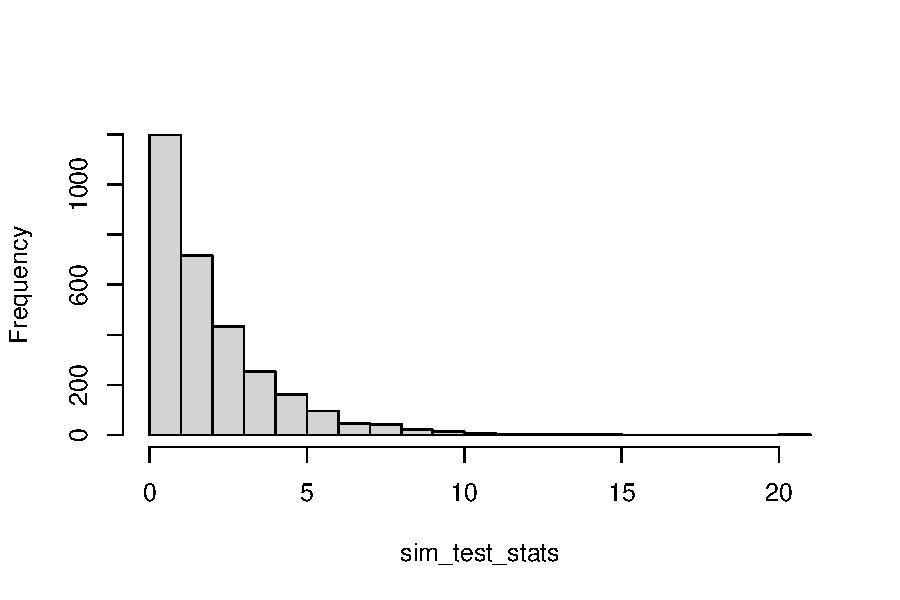
\includegraphics[width=\maxwidth]{figure/listings-unnamed-chunk-27-1} 

}

\end{Schunk}
\begin{goldbox}
	We re-estimate the recombination fraction and expected cell counts \textit{within} the loop replicating what we did to calculate the original test statistic. This is important because it changes the shape of the null distribution. Try for yourself to see what happens when the hypothesised proportions and expectations are fixed.
\end{goldbox}
\subsubsection{Significance}
Let's compare this with the distribution of test statistics that we simulated assuming the null hypothesis is true.
\begin{Schunk}
\begin{Sinput}
n = 400
hyp_probs = c(0.3, 0.2, 0.2, 0.3)
expected_counts  = hyp_probs * n
t0 = sum((y-expected_counts)^2/expected_counts)
t0
\end{Sinput}
\begin{Soutput}
[1] 1.966667
\end{Soutput}
\begin{Sinput}
mean(sim_test_stats >= t0)
\end{Sinput}
\begin{Soutput}
[1] 0.3683333
\end{Soutput}
\begin{Sinput}
hist(sim_test_stats, main = "", breaks = 20)
abline(v = t0, col = "#224099", lwd = 2)
\end{Sinput}


{\centering 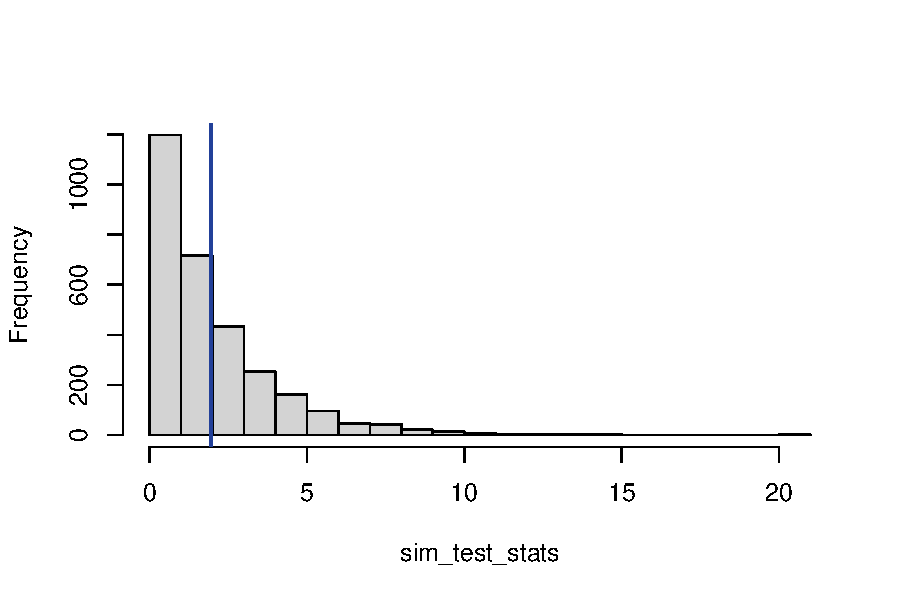
\includegraphics[width=\maxwidth]{figure/listings-unnamed-chunk-28-1} 

}

\end{Schunk}
\begin{itemize}
	\item \textbf{Hypothesis}: The null hypothesis is a coupling linkage model,\( H_0 : p_{AB} = p_{ab} = \frac{1-p}{2} \) and \( p_{Ab} = p_{aB} = \frac{p}{2} \). The alternative that the proportions do not follow a coupling phase linkage model, i.e \( H_1: \) at least one equality does not hold.
	\item \textbf{Assumptions}: independent observations and expected cell counts at least 5, \( e_i = np_{i0} \geq 5 \)
	\item \textbf{Test statistic}: \( T = \sum\limits_{i=1}^{k} \frac{(Y_i - e_i)^2}{e_i} \). Under \( H_0, T \sim \chi^2_2 \) approximately.
	\item \textbf{Observed test statistic}: \( t_0 = 18 \).
	\item \textbf{P-value}: \( P(T\geq t_0) = P(\chi^2_2 \geq 1.97) =  0.37 \)
	\item \textbf{Decision}: Since the p-value is much smaller than 0.05,  so we do not reject the null hypothesis and conclude that the data are consistent with the ``coupling phase'' linkage model.
\end{itemize}
\subsubsection{In R}
\begin{Schunk}
\begin{Sinput}
chisq.test(y, p = p)
\end{Sinput}
\begin{Soutput}

	Chi-squared test for given probabilities

data:  y
X-squared = 1.9667, df = 3, p-value = 0.5794
\end{Soutput}
\end{Schunk}
\begin{tcolorbox}[bluestylecolor]
	\textbf{Note the incorrect degrees of freedom!}
\end{tcolorbox}
\begin{Schunk}
\begin{Sinput}
n = sum(y)
k = length(y)
(ey = n*p)
\end{Sinput}
\begin{Soutput}
[1] 120  80  80 120
\end{Soutput}
\begin{Sinput}
ey >= 5 # check e_i >= 5
\end{Sinput}
\begin{Soutput}
[1] TRUE TRUE TRUE TRUE
\end{Soutput}
\begin{Sinput}
(t0=sum((y-ey)^2/ey))
\end{Sinput}
\begin{Soutput}
[1] 1.966667
\end{Soutput}
\begin{Sinput}
(pval=1 - pchisq(t0, df = k - 1 - 1))
\end{Sinput}
\begin{Soutput}
[1] 0.3740621
\end{Soutput}
\end{Schunk}
\section{Goodness of fit tests for discrete distributions}\label{sec:4}
\subsubsection{Radiation exposure}
The goal in biological dosimetry is to estimate the dose of \textcolor{myred}{\textbf{ionizing radiation}}, absorbed by an exposed individual by using chromosome damage in peripheral lymphocytes.\\
When radiation exposure occurs, the damage in DNA is randomly distributed between cells producing chromosome aberrations. The outcome of interest is the number of aberrations observed. The number of aberrations typically follows a Poisson distribution, the rate of which depends on the dose.\\
The table below shows the number of chromosome aberrations from a patient exposed to radiation after the nuclear accident of Stamboliyski (Bulgaria) in 2011
\begin{table}[H]
	\centering
	\begin{tabular}{@{}lcccccccc@{}}
	\toprule
	Number of aberrations & 0   & 1  & 2  & 3  & 4 & 5 & 6 & 7 \\ \midrule
	Frequency             & 117 & 94 & 51 & 15 & 0 & 0 & 0 & 1 \\ \bottomrule
	\end{tabular}
\end{table}
\begin{greenbox}
	\textbf{How can we check if the random variable generating this data follows a Poisson distribution.}
\end{greenbox}
\subsubsection{Poisson distribution}
A \textbf{Poisson} random variable represents the probability of a given number of events occurring in a fixed interval (e.g. number of events in a fixed period of time) if these event occur independently with some known average rate \( \lambda \) per unit of time.\\
If \( X \) is a Posson random variable with rate parameter \( \lambda \), the probability mass function is:
\[
	P(X = k) = e^{-\lambda} \frac{\lambda^k}{k!}, \quad k=0,1,2,\dotsc,
\]
\begin{Schunk}
\begin{Sinput}
set.seed(8)
rpois(n=10000, lambda = 2) |>
  table() |>
plot(ylab = "Count")	
\end{Sinput}


{\centering 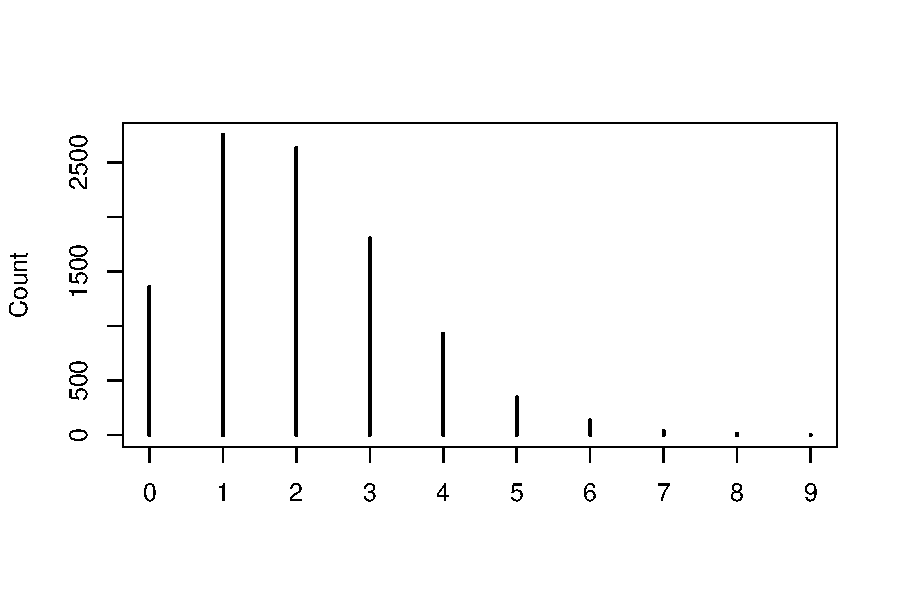
\includegraphics[width=\maxwidth]{figure/listings-unnamed-chunk-31-1} 

}

\begin{Sinput}
rpois(n=10000, lambda = 6) |>
  table() |>
plot(ylab = "Count")
\end{Sinput}


{\centering 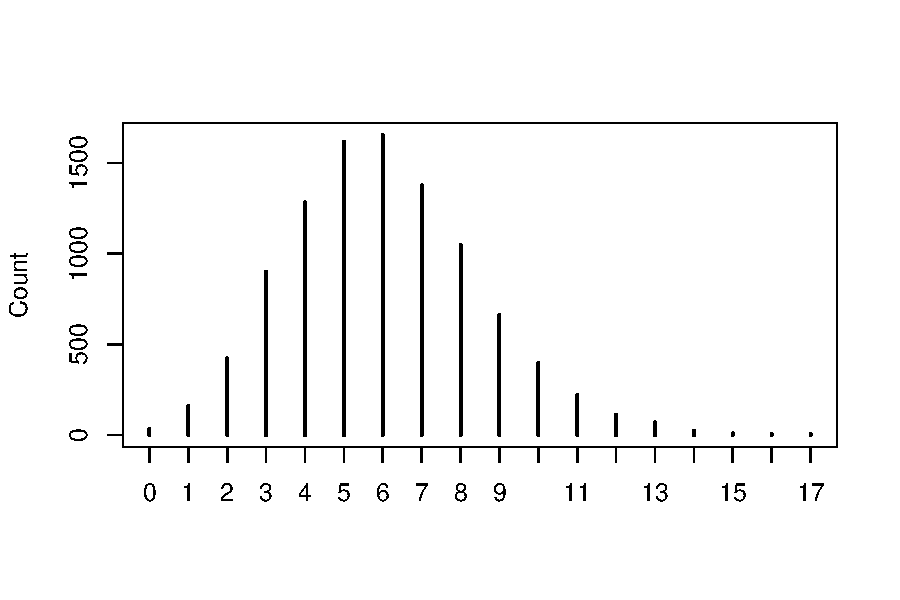
\includegraphics[width=\maxwidth]{figure/listings-unnamed-chunk-31-2} 

}

\end{Schunk}
\subsubsection{Chi-squared tests for discrete distributions}
Suppose we have a sample of observations \( x_1,x_2,\dotsc,x_n \).\\
We want to test whether the sample is taken from a population with a given distribution function \( F_0 (x \mid \theta_1, \theta_2, \dotsc, \theta_h) \) where \( \theta_l \) are parameters of the distribution.\\
We summarise the observed data by tabulating the observed frequencies \( y_i \) for each possible outcome and compare them to the corresponding expected frequencies, \( e_i \) calculate using the expected probabilities, \( p_i \), from the hypothesised distribution, \( F_0 (x \mid \theta_1, \theta_2, \dotsc, \theta_h) \).\\
This is a \textit{general} chi-squared goodness-of-fit test with test statistic,
\[
	T = \sum_{i=1}^{k} \frac{(Y_i - e_i)^2}{e_i} = \sum_{i=1}^{k}\frac{(Y_i - np_i)^2}{np_i},
\]
where \( i = 1,2,\dotsc,k \) iterates over the distinct outcomes.\\
However the model parameters \( \theta_1, \theta_2,\dotsc,\theta_h \) are usually \textbf{unknown} and have to be estimated from the sample.\\
In theis case, the expected probabilities \( p_i \) are replaced by their estimates \( \hat{p}_i \).\\
Then the obseved test statistic is
\[
	t_0 = \sum_{i=1}^{k} \frac{(y_i - n\hat{p}_i)^2}{n \hat{p}_i}
\]
and the approximate p-value is
\[
	P(\chi^2_{k-1-q} \geq t_0).
\]
Note the degrees of freedom are \( k-1-q \) where \( q \) is the number of parameters we need to estimate.
\subsubsection{Radiation exposure}
\begin{itemize}
	\item Let \( X \) be a random variable such that \( X \sim \text{Poisson}\;(\lambda) \).
	\item Let \( y_i \) be the observed frequency of outcome \( i \).
	\item The expected probabilities \( p_i \) are given by the probability mass function,
	\[
		P(X = i) = p_i = e^{-\lambda} \frac{\lambda^i}{i!} \quad\text{for}\; i = 0,1,2,\dotsc,
	\]
	where \( p_i \) denote the probability of the number of chromosome aberrations in the \( i \)th category.
	\item Note that for a Posson distribution both \( \mathrm{\mathrm{E}}(X) \) and \( \var(X) \) are equal to the parameter \( \lambda \).
	\item We need to estimate \( \lambda \) by the sample mean: \( \hat{\lambda} = \overline{x} = 248 / 278 = 0.89 \).
	\begin{table}[H]
		\centering
		\begin{tabular}{@{}l|crrr@{}}
		\toprule
		\( i \) & \( y_i \) &  \( \hat p_i=e^{- \hat{\lambda}}\hat{\lambda}^i /i! \) & \( \hat{e}_i = n\hat{p}_i \) & \( (y_i-\hat{e}_{i})^2/\hat{e}_{i} \) \\ \addlinespace[0.5em] \midrule  
		\( 0 \) &  117 &  \( \dfrac{0.89^0 e^{-0.89}}{0!} = 0.4098 \) & \( 278 \times 0.4098 = 113.92 \) & \( \dfrac{(117-113.92)^2}{113.92} = 0.08 \)  \\  \addlinespace[0.5em] 
		\( 1 \) &  94  &  \( \dfrac{0.89^1 e^{-0.89}}{1!} = 0.3656 \) & \( 278 \times 0.3656 = 101.63 \) & \( \dfrac{(94-101.63)^2}{101.63} = 0.57 \)    \\  \addlinespace[0.5em]
		\( 2 \) &  51  &  \( \dfrac{0.89^2 e^{-0.89}}{2!} = 0.1631 \) & \( 278 \times 0.1631 = 45.33 \) & \( \dfrac{(51-45.33)^2}{45.33} = 0.71 \)  \\ \addlinespace[0.5em]   
		\( 3 \) &    15  &  \( \dfrac{0.89^3 e^{-0.89}}{3!} = 0.0485 \) & \( 278 \times 0.0485 = 13.48 \) & \( \dfrac{(15-13.48)^2}{13.48} = 0.17 \)  \\ \addlinespace[0.5em]   
		\( 4 \) &    0     &  \( \dfrac{0.89^4 e^{-0.89}}{4!} = 0.0108 \) & \( 278 \times 0.0108 = 3.01 \) & \( \dfrac{(0-3.01)^2}{3.01} = 3.01 \)  \\ \addlinespace[0.5em]  
		\( 5 \) &    0     &  \( \dfrac{0.89^5 e^{-0.89}}{5!} = 0.0019 \)& \( 278 \times 0.0019 = 0.54 \) & \( \dfrac{(0-0.54)^2}{0.54} = 0.54 \)  \\ \addlinespace[0.5em]  
		\( 6 \) &    0     &  \( \dfrac{0.89^6 e^{-0.89}}{6!} = 0.0003 \)& \( 278 \times 0.0003 = 0.08 \) & \( \dfrac{(0-0.08)^2}{0.08} = 0.08 \)  \\ \addlinespace[0.5em]  
		\( \geq 7 \) &  1 &  0.00004 & \( 278 \times 0.00004 = 0.01 \) & \( \dfrac{(1 - 0.01)^2}{0.01}=   96.40 \) \\
		\midrule  
		Total &  278  & 1 & 278 & 101.56 \\ \bottomrule
		\end{tabular}
	\end{table}
	\item But wait! There are a number of cells where the expected number of counts is less than 5 which violates an assumption.
	\item We combine the last five classes so that the final group is \( \geq 3 \) with observed frequency \( y_{\geq 3} = 15+1 = 16 \), the expected count is \( \hat{e}_{\ge3} = 13.48+3.01+0.54+0.08+0.01 = 17.12 \):
	\begin{table}[H]
		\centering
		\begin{tabular}{@{}l|crrr@{}}
		\toprule
		\( i \) & \( y_i \) &  \( \hat p_i=e^{- \hat{\lambda}}\hat{\lambda}^i /i! \) & \( \hat{e}_i = n\hat{p}_i \) & \( (y_i-\hat{e}_{i})^2/\hat{e}_{i} \) \\ \addlinespace[0.5em]\midrule  
		\( 0 \) &  117 &  \( \dfrac{0.89^0 e^{-0.89}}{0!} = 0.4098 \) & \( 278 \times 0.4098 = 113.92 \) & \( \dfrac{(117-113.92)^2}{113.92} = 0.08 \)  \\ \addlinespace[0.5em]  
		\( 1 \) &  94  &  \( \dfrac{0.89^1 e^{-0.89}}{1!} = 0.3656 \) & \( 278 \times 0.3656 = 101.63 \) & \( \dfrac{(94-101.63)^2}{101.63} = 0.57 \)    \\ \addlinespace[0.5em] 
		\( 2 \) &  51  &  \( \dfrac{0.89^2 e^{-0.89}}{2!} = 0.1631 \) & \( 278 \times 0.1631 = 45.33 \) & \( \dfrac{(51-45.33)^2}{45.33} = 0.71 \)  \\ \addlinespace[0.5em]
		\( \geq 3 \) & 16 & \( 1-0.4098-0.3656-0.1631 = 0.0615 \) & \( 278 \times 0.015 = 17.12 \) & \( \dfrac{(16 - 17.12)^2}{17.12} = 0.07 \) \\ \midrule
		Total &  278  & 1 & 278 & 1.43 \\ \bottomrule
		\end{tabular}
	\end{table}
	\item The final observed test statistic is, \( t_0 = 0.08 + 0.57 + 0.71 + 0.07 = 1.43 \) 
	\item \textbf{Hypothesis}: \( H_0 \): the data follow a Poisson distribution vs \( H_1 \): the data do not follow from a Possion distribution.
	\item \textbf{Assumptions}: The expected frequencies, \( e_i = np_i \geq 5 \) . Observations are independent.
	\item \textbf{Test statistic}: \( T=\sum\limits_{i=1}^k \frac{(Y_i-n p_i)^2}{n p_i} \). Under \( H_0 \), \( T \sim \chi^2_2 \) approximately.
	\item \textbf{Observed test statistic}: \( t_0 = 1.43 \) 
	\item \textbf{P-value}: \( P(T \geq t_0) = P(\chi_2^2 \geq 1.43) = 0.49 \) 
	\item \textbf{Decision}: Since the p-value is greater than 0.05, we do not reject the null hypothesis. The data are consistent with a Poisson distribution.
\end{itemize}
\begin{goldbox}
	We don't conclude that \( H_0 \) is true, just that the data are consistent with \( H_0 \). This is a subtle distinction.
\end{goldbox}
If we wanted to implement this ``manually'' in R:
\begin{Schunk}
\begin{Sinput}
y = c(117, 94, 51, 15, 0, 0, 0, 1) # input the observed counts
x = 0:7 # define the corresponding groups
n = sum(y) # total number of samples (sample size)
k = length(y) # number of groups
(lam = sum(y * x)/n) # estimate the lambda parameter
\end{Sinput}
\begin{Soutput}
[1] 0.8920863
\end{Soutput}
\begin{Sinput}
p = dpois(x, lambda = lam) # obtain the p_i from the Poisson pmf
p
\end{Sinput}
\begin{Soutput}
[1] 4.097999e-01 3.655769e-01 1.630631e-01 4.848878e-02 1.081404e-02
[6] 1.929412e-03 2.868670e-04 3.655859e-05
\end{Soutput}
\begin{Sinput}
p[8] = 1 - sum(p[1:7]) # redefine the 8th element P(>=7) NOT P(7)
round(p, 5)
\end{Sinput}
\begin{Soutput}
[1] 0.40980 0.36558 0.16306 0.04849 0.01081 0.00193 0.00029 0.00004
\end{Soutput}
\begin{Sinput}
(ey = n * p) # calculate the expected frequencies
\end{Sinput}
\begin{Soutput}
[1] 113.92436722 101.63037076  45.33153228  13.47988010   3.00630420
[6]   0.53637658   0.07974904   0.01141984
\end{Soutput}
\begin{Sinput}
ey >= 5 #check assumption e_i >= 5 not all satisfied
\end{Sinput}
\begin{Soutput}
[1]  TRUE  TRUE  TRUE  TRUE FALSE FALSE FALSE FALSE
\end{Soutput}
\end{Schunk}
Collapsing categories, so that the assumptions are met:
\begin{Schunk}
\begin{Sinput}
(yr = c(y[1:3], sum(y[4:8])))  # reduced category counts
\end{Sinput}
\begin{Soutput}
[1] 117  94  51  16
\end{Soutput}
\begin{Sinput}
(eyr = c(ey[1:3], sum(ey[4:8])))  # reduced category expected cell counts
\end{Sinput}
\begin{Soutput}
[1] 113.92437 101.63037  45.33153  17.11373
\end{Soutput}
\begin{Sinput}
all(eyr >= 5)  # check that all expected cell counts are >= 5
\end{Sinput}
\begin{Soutput}
[1] TRUE
\end{Soutput}
\begin{Sinput}
(pr = c(p[1:3], sum(p[4:8])))  # reduced category hypothesised probabilities
\end{Sinput}
\begin{Soutput}
[1] 0.40979988 0.36557687 0.16306307 0.06156018
\end{Soutput}
\begin{Sinput}
kr = length(yr)  # number of combined classes
(t0 = sum((yr - eyr)^2/eyr))  # test statistic
\end{Sinput}
\begin{Soutput}
[1] 1.43721
\end{Soutput}
\begin{Sinput}
(pval = 1 - pchisq(t0, df = kr - 1 - 1))  # p-value
\end{Sinput}
\begin{Soutput}
[1] 0.4874317
\end{Soutput}
\end{Schunk}
What if we try to use \lstinline|chisq.test()|?
\begin{Schunk}
\begin{Sinput}
chisq = chisq.test(yr, p = pr)
chisq
\end{Sinput}
\begin{Soutput}

	Chi-squared test for given probabilities

data:  yr
X-squared = 1.4372, df = 3, p-value = 0.6968
\end{Soutput}
\end{Schunk}
The degrees of freedom are wrong, is there a slightly easier way to get the right answer?
\begin{Schunk}
\begin{Sinput}
chisq$statistic
\end{Sinput}
\begin{Soutput}
X-squared 
  1.43721 
\end{Soutput}
\begin{Sinput}
pchisq(unname(chisq$statistic), df = 2, lower.tail = FALSE)
\end{Sinput}
\begin{Soutput}
[1] 0.4874317
\end{Soutput}
\end{Schunk}
Visualising the comparison between observed and expected counts.
\begin{Schunk}
\begin{Sinput}
par(mfrow = c(1, 2))
xr = c("0", "1", "2", ">=3")  # group labels
barplot(yr, names.arg = xr, main = "Observed frequency")
barplot(eyr, names.arg = xr, main = "Expected frequency")
\end{Sinput}


{\centering 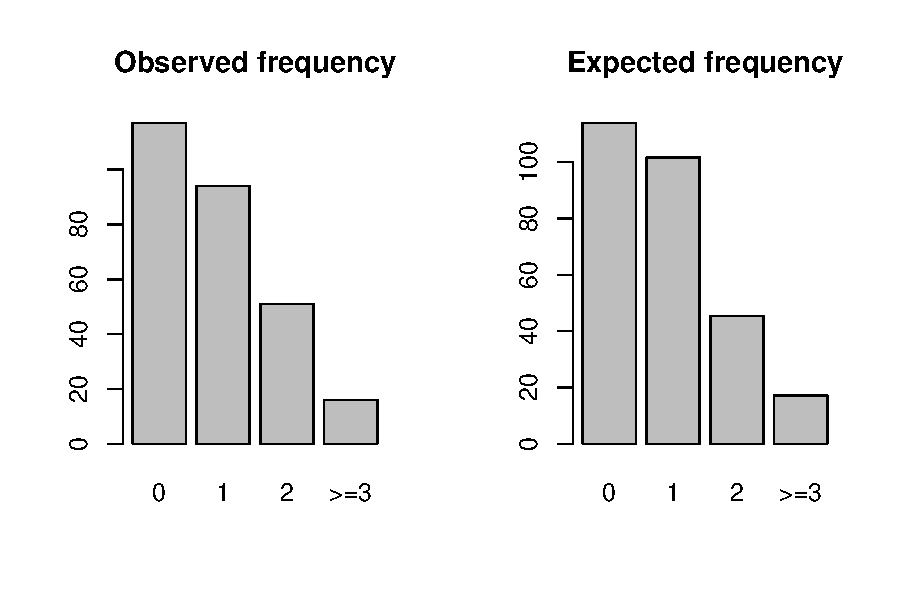
\includegraphics[width=\maxwidth]{figure/listings-unnamed-chunk-36-1} 

}

\end{Schunk}
Visualising the comparison between observed and expected counts.
\begin{Schunk}
\begin{Sinput}
dat = tibble::tibble(
  aberrations = factor(
    xr, 
    levels = c("0","1","2",">=3")
  ),
  observed = yr,
  expected = eyr
)
dat |> ggplot() + 
  aes(x = aberrations, y = observed) + 
  geom_col(alpha = 0.5) + 
  geom_point(aes(y = eyr),
             colour = "#224099") + 
  labs(y = "Count", 
       x = "Number of aberrations") + 
  theme_classic()
\end{Sinput}


{\centering 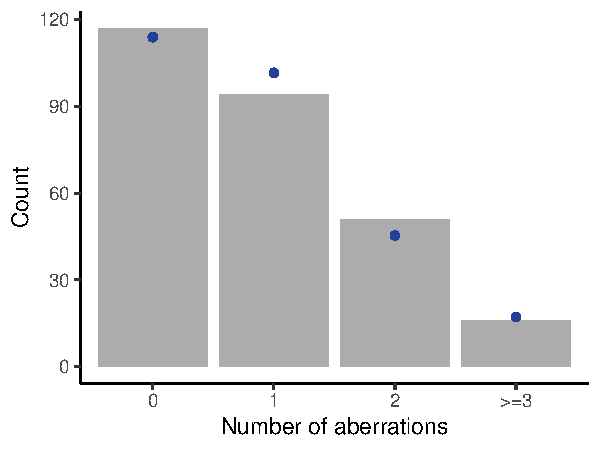
\includegraphics[width=\maxwidth]{figure/listings-unnamed-chunk-37-1} 

}

\end{Schunk}
\section{Measures of performance}\label{sec:5}
\subsection{Types of errors}
\subsubsection{Test result vs actual status}
In general, \textbf{positive} = identified and \textbf{negative} = rejected. Therefore:
\textbf{True positive} = correctly identified \\
\textbf{False positive} = incorrectly identified \\
\textbf{True negative} = correctly rejected \\
\textbf{False negative} = incorrectly rejected \\
We can summarise this in a table:
\begin{table}[H]
	\centering
	\begin{tabular}{@{}c|cc@{}}
	\toprule
						   & \textbf{Actual positive} & \textbf{Actual negative} \\ \midrule
	\textbf{Test positive}  & True positive (TP)       & False positive (FP)      \\
	\textbf{Test negative} & False negative (FN)      & True negative (TN)       \\ \bottomrule
	\end{tabular}
\end{table}
\subsubsection{Breast cancer}
\begin{table}[H]
	\centering
	\begin{tabular}{@{}c|cc@{}}
	\toprule
						   & \textbf{Have breast cancer} & \textbf{Does not have breast cancer} \\ \midrule
	\textbf{Mammogram returns a positive test result} & True positive (TP)       & False positive (FP)      \\
	\textbf{Mammogram returns a positive test result} & False negative (FN)      & True negative (TN)       \\ \bottomrule
	\end{tabular}
\end{table}
\begin{itemize}
	\item \textbf{True positive}: Mammogram returns a positive test result and you actually have breast cancer
	\item \textbf{False positive}: Mammogram returns a positive test result but you don't actually have breast cancer
	\item \textbf{False negative}: Mammogram returns a negative test result but you do actually have breast cancer
	\item \textbf{True negative}: Mammogram returns a negative test result and you don't actually have breast cancer
\end{itemize}
\begin{greenbox}
	\textbf{What's worse? False negative (FN) or false positive (FP)?}
\end{greenbox}
\subsubsection{Extra notation}
Let's formalise this. Let,
\begin{itemize}
	\item \textcolor{mygreen}{\( D^+ \)} be the event that an individual \textbf{has} a particular disease. The \textbf{prevalence} is the marginal probability of disease, \( P(D^+) \)
	\item \textcolor{mygreen}{\( D^- \)} be the event that an individual \textbf{does not} have a particular disease.
	\item \textcolor{myred}{\( S^+ \)} represent a positive screening test result or a symptom being present.
	\item \textcolor{myred}{\( S^- \)} represent a negative screening test result or no symptom.
\end{itemize}
With this notation, we can start to quantify the influence of a risk factor or screening test \( (S) \) in the disease outcome \( (D) \).
\begin{table}[H]
	\centering
	\begin{tabular}{@{}c|cc@{}}
	\toprule
	                                & \textcolor{mygreen}{\textbf{Actual positive \( D+ \)}} & \textcolor{mygreen}{\textbf{Actual negative \( D- \)}} \\ \midrule
	\textcolor{myred}{\textbf{Test positive \( S+ \)}}  & True positive (TP)       & False positive (FP)      \\
	\textcolor{myred}{\textbf{Test negative \( S- \)}} & False negative (FN)      & True negative (TN)       \\ \bottomrule
	\end{tabular}
\end{table}
\begin{table}[H]
	\centering
	\begin{tabular}{@{}cccc@{}}
	\toprule
	& \textcolor{mygreen}{\textbf{Actual positive \( D+ \)}} & \textcolor{mygreen}{\textbf{Actual negative \( D- \)}} \\ \midrule
	\textcolor{myred}{\textbf{Test positive \( S+ \)}}  & \( a \)   & \( b \)   & \( a + b \) \\
	\textcolor{myred}{\textbf{Test negative \( S- \)}} & \( c \)   & \( d \)   & \( c + d \) \\
													   & \( a+c \) & \( b+d \) & \( a + b + c + d \) \\ \bottomrule
	\end{tabular}
\end{table}
\begin{itemize}
	\item \textbf{False negative rate}: \( P(S^- \mid D^+) = \frac{c}{a + c} \) 
	\item \textbf{False positive rate}: \( P(S^+ \mid D^-) = \frac{b}{b + d} \)
	\item \textbf{Sensitivity / Recall}: \( P(S^+ \mid D^+) = \frac{a}{a + c} \), the probability that the test is positive given that the subject actually has the disease
	\item \textbf{Specificity}: \( P(S^- \mid D^-) = \frac{d}{b + d} \), the probability that the test is negative given that the subject does not have the disease
	\item \textbf{Positive predictive value/Precision}: \( P(D^+ \mid S^+) = \frac{a}{a + b} \), the probability that the subject has the disease given that the test is positive
	\item \textbf{Negative predictive value}: \( P(D^- \mid S^-) = \frac{d}{c + d} \), the probability that the subject does not have the disease given that the test is negative
	\item \textbf{Accuracy}: \( \frac{a + d}{a + b + c + d} \) 
\end{itemize}
\subsubsection{Breast cancer}
\begin{table}[H]
	\centering
	\begin{tabular}{@{}cccc@{}}
	\toprule
	& \textcolor{mygreen}{\textbf{Actual positive \( D+ \)}} & \textcolor{mygreen}{\textbf{Actual negative \( D- \)}} \\ \midrule
	\textcolor{myred}{\textbf{Test positive \( S+ \)}} & 9  & 99   & 108 \\
	\textcolor{myred}{\textbf{Test negative \( S- \)}} & 1  & 891  & 892 \\
													   & 10 & 990 & 1000 \\ \bottomrule
	\end{tabular}
\end{table}
Prevalence: 1\% (10/1000)\\
Sensitivity: 90\% (9/10)\\
Specificity: 90\% (891/990)\\
\textbf{Positive predictive value (or precision)}
\[
	P(D^+ \mid s^+) = \frac{9}{9+99} = 0.08
\]
\subsection{Conditional probability}
\subsubsection{Motivation}
It's been suggested that lawn bowls is one of the most dangerous sports in the world (highest death rates).
\begin{greenbox}
	\textbf{Given that you're a young adult, should you be worried about playing?}
\end{greenbox}
\textbf{Conditional on being a young adult}, the risk of playing lawn bowls is very small.\\
Even though the probability of dying while playing lawn bowls is higher than many other sports, the overwhelming majority of lawn bowl related deaths are linked to the extreme age of the player.
\subsubsection{Definition}
\begin{itemize}
	\item Let \( B \) be an event so that \( P(B) > 0 \)
	\item The conditional probability of an event \( A \) given that \( B \) has occured is
	\[
		P(A \mid B) = \frac{P(A \cap B)}{P(B)}
	\]
	Rearranging, we also have
	\begin{itemize}
		\item \( P(A \cap B) = P(A \mid B)P(B) \) 
		\item \( P(A \cap B) = P(B \mid A)P(a) \) 
	\end{itemize}
	\item For the \textit{classical definition of probability} where we have a finite number of equally likely outcomes, then
	\begin{itemize}
		\item \( P(A) \) is the \textit{proportion} of outcomes in the subset \( A \) 
		\item \( P(B) \) is the \textit{proportion} of outcomes in the subset \( B \) 
		\item \( P(A \mid B) \) is the \textit{proportion of outcomes in} \( B \) \textit{that are also in} \( A \) 
	\end{itemize}
\end{itemize}
\subsubsection{Bayes' rule}
Bayes' rule allows us to reverse the conditioning set provided that we know some marginal probabilities,
\begin{align*}
		P(B \mid A) & = \frac{P(B\cap A)}{P(A)} \\
		& = \frac{P(A \mid B) P(B)}{P(A \mid B) P(B) + P(A \mid B^c)P(B^c)}.
\end{align*}
where \( B^{c} \) is the vent that \( B \) doesn't occur.\\
Note that we've used the \textcolor{myred}{law of total probability}
\[
	P(A) = P(A\cap B) + P(A\cap B^c) =  P(A \mid B) P(B) + P(A \mid B^c)P(B^c)
\]
\subsubsection{Efficacy of HIV tests}
A study comparing the efficacy of HIV tests, reports on an experiment which concluded that HIV antibody tests have a \textbf{sensitivity} of 99.7\% and a \textbf{specificity} of 98.5\%. Suppose that a subject, from a population with a .1\% \textbf{prevalence} of HIV, receives a positive test result. What is the positive predictive value?
\begin{itemize}
	\item Mathematically, we want \( P(D^+ \mid S^+) \) given the sensitivity, \( P(S^+ \mid D^+) =.997 \), the specificity, \( P(S^- \mid D^-) = 0.985 \), and the prevalence \( P(D^+) = .001 \)
	\[
		P(D^+ \mid S^+) = \frac{P(S^+ \mid D^+)P(D^+)}{P(S^+ \mid D^+)P(D^+) + P(S^+ \mid D^-)P(D^-)}
	\]
	Need to find:
	\item \( P(D^-) = 1-P(D^+) = 1- 0.001 = 0.999 \)
	\item \( P(S^+ \mid D^-) = 1-P(S^- \mid D^-) = 1 - 0.985 = 0.015 \) 
\end{itemize}
\begin{align*}
	P(D^+ \mid S^+) & = \frac{P(S^+ \mid D^+)P(D^+)}{P(S^+ \mid D^+)P(D^+) + P(S^+ \mid D^-)P(D^-)}\\
	& = \frac{.997\times .001}{.997 \times .001 + .015 \times .999}  = 0.062
\end{align*}
In this population a positive test result only suggests a 6.2\% probability that the subject has the disease I.e. the positive predictive value is 6.2\% for this test.
\begin{itemize}
	\item The low positive predictive value is due to low prevalence of disease and the somewhat modest specificity
	\item Suppose it was known that the subject was an intravenous drug user and routinely had intercourse with an HIV infected partner
	\item The evidence implied by a positive test result does not change because of the prevalence of disease in the subject's population, only our interpretation of that evidence changes
\end{itemize}
\subsection{Evaluating classification models}
\subsubsection{Evaluating a classification model}
Imagine a very simple classification model looking to classify a particular type of deformation, kyphosis, in children who have had corrective spinal surgery Chambers \& Hastie (1991).
The \textbf{outcome} is absence or presence of kyphosis after the operation.\\
The \textbf{predictor} is the number of the topmost vertebra operated on.
\begin{itemize}
	\item If the highest vertebrae operated on was 9th or higher, we predict that kyphosis will be absent after surgery.
	\item If the highest vertebrae operated on was 8th or lower, we predict that kyphosis will be present after surgery.
\end{itemize}
The data can be found in the \lstinline|kyphosis| data frame that comes with the \textbf{rpart} package.
\begin{Schunk}
\begin{Sinput}
data(kyphosis, package = "rpart")
dplyr::glimpse(kyphosis)
\end{Sinput}
\begin{Soutput}
Rows: 81
Columns: 4
$ Kyphosis <fct> absent, absent, present, absent, absent, absent, absent, abse~
$ Age      <int> 71, 158, 128, 2, 1, 1, 61, 37, 113, 59, 82, 148, 18, 1, 168, ~
$ Number   <int> 3, 3, 4, 5, 4, 2, 2, 3, 2, 6, 5, 3, 5, 4, 3, 3, 6, 5, 5, 4, 2~
$ Start    <int> 5, 14, 5, 1, 15, 16, 17, 16, 16, 12, 14, 16, 2, 12, 18, 16, 1~
\end{Soutput}
\begin{Sinput}
kyphosis = kyphosis |> 
  dplyr::mutate(
    prediction = if_else(Start >= 9, 
                         "Predict absent", 
                         "Predict present")
  )
table(kyphosis$prediction, kyphosis$Kyphosis)
\end{Sinput}
\begin{Soutput}
                 
                  absent present
  Predict absent      56       6
  Predict present      8      11
\end{Soutput}
\end{Schunk}
For our prediction model, define \( D^-, D^-, S^+, S^- \) and find the
\begin{itemize}
	\item accuracy
	\item sensitivity
	\item specificity
	\item false negative rate
	\item false positive rate
	\item positive predictive value
	\item negative predictive value
\end{itemize}
\begin{greenbox}
	\textbf{Reordering the rows and columns in the table might help!}
\end{greenbox}
We can use the \textbf{yardstick} package from the \textbf{tidymodels} suite of packages to do this for us.
\begin{Schunk}
\begin{Sinput}
conf_mat = kyphosis |> 
  dplyr::mutate(
    prediction = if_else(Start >= 9, 
                         "absent", 
                         "present"),
    Kyphosis = factor(Kyphosis, levels = c("present", "absent")),
    prediction = factor(prediction, levels = c("present", "absent"))
  ) |> 
  yardstick::conf_mat(truth = Kyphosis, estimate = prediction)
conf_mat
\end{Sinput}
\begin{Soutput}
          Truth
Prediction present absent
   present      11      8
   absent        6     56
\end{Soutput}
\begin{Sinput}
summary(conf_mat) |> 
  select(-2) |> 
  gt::gt() |> 
  gt::fmt_percent(columns = 2,
                  decimals = 1)
\end{Sinput}
\begin{longtable}{lr}
\toprule
.metric & .estimate \\ 
\midrule\addlinespace[2.5pt]
accuracy & $82.7\%$ \\ 
kap & $50.0\%$ \\ 
sens & $64.7\%$ \\ 
spec & $87.5\%$ \\ 
ppv & $57.9\%$ \\ 
npv & $90.3\%$ \\ 
mcc & $50.2\%$ \\ 
j\_index & $52.2\%$ \\ 
bal\_accuracy & $76.1\%$ \\ 
detection\_prevalence & $23.5\%$ \\ 
precision & $57.9\%$ \\ 
recall & $64.7\%$ \\ 
f\_meas & $61.1\%$ \\ 
\bottomrule
\end{longtable}
\begin{Sinput}
autoplot(conf_mat, type = "heatmap")
\end{Sinput}


{\centering 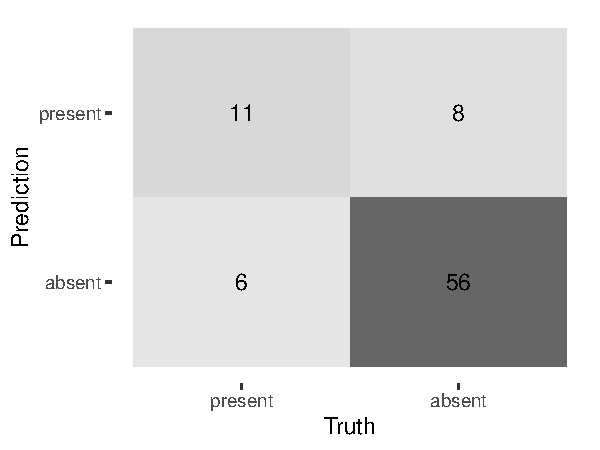
\includegraphics[width=\maxwidth]{figure/listings-unnamed-chunk-39-1} 

}

\end{Schunk}


\section{Measures of risk}\label{sec:6}
\subsection{Motivating examples}
\subsubsection{Asthma and hay fever}
A large group of infants with mild respiratory problems (but asthma free) is split into those with a family history of hay fever, and those without.\\
Random samples of 85 from the first group and 405 from the second group are selected for special study. Of these, the number diagnosed with asthma by the age of 12 are 25 and 70 respectively.
\begin{table}[H]
	\centering
	\begin{tabular}{@{}ccc|c@{}}
	\toprule
				 & Asthma & No Asthma &     \\ \midrule
	Hay fever    & 25    & 60        & 85  \\
	No hay fever & 70    & 335       & 405 \\ \midrule
				 & 95    & 395       &     \\ \bottomrule
	\end{tabular}
\end{table}
\begin{greenbox}
	\textbf{Does a family history of hay fever increase the risk of developing asthma?}
\end{greenbox}
\subsubsection{Hodgkin's disease and tonsillectomies}
Vianna et al. (1971) collected data on a group of \textbf{101 patients suffering from Hodgkin's disease} and a comparable control group of \textbf{107 non-Hodgkin's patients}.\\
They were interested in the effect of tonsil tissue as a barrier to Hodgkin's disease. They found that in the Hodgkin's disease group, there had been 67 tonsillectomies. The corresponding figure for the non-Hodgkin's patients was 43.
\begin{table}[H]
	\centering
	\begin{tabular}{@{}ccc|c@{}}
		\toprule
					  & \multicolumn{2}{c}{Hodgkin's disease} &     \\
		Tonsillectomy & Yes                & No                &     \\ \midrule
		Yes           & 67                 & 43                & 110 \\
		No            & 34                 & 64                & 98  \\ \midrule
					  & 101                & 107               &     \\ \bottomrule
		\end{tabular}
\end{table}
\begin{greenbox}
	\textbf{Does having a tonsillectomy increase your risk of developing Hodgkin's disease?}
\end{greenbox}
\subsubsection{Notation}
How a study is conducted over time will affect various conditional probabilities.\\
To illustrate this we will use the following symbols.
\begin{itemize}
	\item \textcolor{mygreen}{\( D^+ \)} is the event that an individual \textbf{has} a particular disease.
	\item \textcolor{mygreen}{\( D^- \)} is the event that an individual \textbf{does not have} a particular disease.
	\item \textcolor{myred}{\( R^+ \)} is the event that an individual \textbf{has} a risk factor.
	\item \textcolor{myred}{\( R^- \)} is the event that an individual \textbf{does not have} a risk factor.
\end{itemize}
\subsection{Prospective studies}
\subsubsection{Prospective (or cohort study) studies}
A study design where one or more samples (called cohorts) are followed prospectively and subsequent status evaluations with respect to a disease or outcome are conducted to determine which initial participants exposure characteristics (risk factors) are associated with it.\\
As the study is conducted, an outcome from participants in each cohort is measured and relationships with specific characteristics determined.
\begin{goldbox}
\begin{itemize}
	\item A \textbf{prospective study} is based on subjects who are initially identified as \textit{disease-free} and classified by presence or absence of a \textit{risk factor}.
	\item A random sample from each group is followed in time (prospectively) until eventually classified by disease outcome.
\end{itemize}
\end{goldbox}
\subsubsection{Fictious example}
\begin{itemize}
	\item A \textbf{prospective study }was designed to assess the impact of sun exposure on skin damage in beach volleyball players.
	\item During a weekend tournament, players from one team wore waterproof, SPF 35 sunscreen, while players from the other team did not wear any sunscreen.
	\item At the end of the volleyball tournament players' skin from both teams was analyzed for texture, sun damage, and burns.
	\item Comparisons of skin damage were then made based on the use of sunscreen.
	\item The analysis showed a significant difference between the cohorts in terms of the skin damage.
\end{itemize}
\subsubsection{Asthma}
A large group of infants with mild respiratory problems (but asthma free) is split into those with a family history of hay fever, \textcolor{myred}{\( R^+ \)}, and those without, \textcolor{myred}{\( R^- \)}. Random samples of 85 from the first group and 405 from the second group are selected for special study. Of these, the number diagnosed with asthma by the age of 12, \textcolor{mygreen}{\( D^+ \)}, are 25 and 70 respectively.
\begin{table}[H]
	\centering
	\begin{tabular}{@{}lccr@{}}
	\toprule
				 														 & \textcolor{mygreen}{\textbf{\( D^+ \) Asthma by age 12}} & \textcolor{mygreen}{\textbf{\( D^- \) No Asthma by age 12}} & \textbf{Total}    \\ \midrule
	\textcolor{myred}{\textbf{\( R^+ \) Family History of Hay fever}}    & 25    		  											& 60        		                                          & \textcolor{myred}{\textbf{85}}  \\
	\textcolor{myred}{\textbf{\( R^- \) No family history of hay fever}} & 70    		  											& 335       		                                          & \textcolor{myred}{\textbf{405}} \\ \midrule
	\textbf{Total} 													     & \textbf{95}    											& \textbf{395}                                                & \textbf{490} \\ \bottomrule
	\end{tabular}
\end{table}
\begin{itemize}
	\item Risk factor is \textcolor{myred}{\textbf{family history of hay fever}}
	\item Disease is \textcolor{mygreen}{\textbf{asthma by age 12}}
\end{itemize}
\begin{goldbox}
	In a prospective study, the \textcolor{myred}{\textbf{number of participants in each of the risk factor groups (row totals)}} is fixed by design.
\end{goldbox}
\subsection{Retrospective studies}
\subsubsection{Retrospective (or case control) stzudies}
A study that compares patients who have a disease or outcome of interest (cases) with patients who do not have the disease or outcome (controls), and looks back retrospectively to compare how frequently the exposure to a risk factor is present in each group to determine the relationship between the risk factor and the disease.
\begin{goldbox}
	A \textbf{retrospective study} is based on random samples from each of the two \textit{outcome categories} which are followed back (retrospectively) to determine the presence or absence of the \textit{risk factor} for each individual.
\end{goldbox}
\subsubsection{Fictious example}
\begin{itemize}
	\item There is a suspicion that zinc oxide, the white non-absorbent sunscreen traditionally worn by lifeguards is more effective at preventing sunburns that lead to skin cancer than absorbent sunscreen lotions.
	\item A \textbf{retrospective study} was conducted to investigate if exposure to zinc oxide is a more effective skin cancer prevention measure.
	\item The study involved comparing a group of former lifeguards that had developed cancer on their cheeks and noses (cases) to a group of lifeguards without this type of cancer (controls) and assess their prior exposure to zinc oxide or absorbent sunscreen lotions.
	\item This study would be \textbf{retrospective} in that the former lifeguards would be asked to recall which type of sunscreen they used on their face and approximately how often.
\end{itemize}
\subsubsection{Hodgkin's disease}
Vianna et al. (1971) collected data on a group of 101 patients suffering from Hodgkin's disease, \textcolor{mygreen}{\( D^+ \)}, and a comparable control group of 107 non-Hodgkin's patients, \textcolor{mygreen}{\( D^- \)}.  They were interested in the effect of tonsil tissue as a barrier to Hodgkin's disease. They found that in the \textcolor{mygreen}{\( D^+ \)} group, there had been 67 tonsillectomies, \textcolor{myred}{\( R^+ \)}. The corresponding figure for the \textcolor{mygreen}{\( D^- \)} group was 43.
\begin{table}[H]
	\centering
	\begin{tabular}{@{}lccr@{}}
	\toprule
				 										   & \textcolor{mygreen}{\textbf{\( D^+ \) Hodgkin's}} & \textcolor{mygreen}{\textbf{\( D^- \) Non-Hodgkin's}} & \textbf{Total}    \\ \midrule
	\textcolor{myred}{\textbf{\( R^+ \) Tonsillectomy}}    & 67    		  									   & 43        		                                       & \textbf{110}  \\
	\textcolor{myred}{\textbf{\( R^- \) No Tonsillectomy}} & 34    		  									   & 64      		                                       & \textbf{98} \\ \midrule
	\textbf{Total} 										   & \textcolor{mygreen}{\textbf{101}}				   & \textcolor{mygreen}{\textbf{107}}                     & \textbf{208} \\ \bottomrule
	\end{tabular}
\end{table}
\begin{itemize}
	\item Risk factor is \textcolor{myred}{\textbf{tonsillectomy}}
	\item Disease is \textcolor{mygreen}{\textbf{Hodgkin's disease}}
\end{itemize}
In a retrospective study the numbers \textcolor{mygreen}{\textbf{highlighted in green}} are fixed by design.
\subsection{Estimating population proportions}
Suppose
\begin{itemize}
	\item we have a large (but finite) population containing objects/individuals of two different types (say type 0 and type 1);
	\item it is desired to determine or at least estimate the overall proportion of type 1 but it is not feasible to examine every object/individual.
\end{itemize}
If we can take a random sample from the population then we can use the sample proportion of type 1 as an estimate of the population proportion of type 1.\\
Extending this idea, consider two events \( A \) and \( B \),
\begin{itemize}
	\item If we can take a random sample from the whole population, we can estimate \( P(A) \) using the observed sample proportion with attribute \( A \).
	\item If we can take a random sample from the subpopulation defined by \( B \), we can estimate \( P(A \mid B) \) using the observed sample proportion (of the subpopulation) with attribute \( A \).
\end{itemize}
\subsubsection{Application to prospective and retrospective studies}
In both kinds of study we have
\begin{itemize}
	\item a population;
	\item a subpopulation/attribute determined by a risk factor \( R^+ \) (with complementary subpopulation/attribute \( R^- \));
	\item an subpopulation/attribute determined by having/developing the disease \( D^+ \) (with complementary subpopulation/attribute \( D^- \))
\end{itemize}
The labels ``subpopulation'' and ``attribute'' here are mathematically equivalent (they both mean event).\\
The main difference between prospective and retrospective studies are which (sub)populations we can sample from.
\subsubsection{Prospective study}
In a \textbf{prospective study} we take two random samples:
\begin{itemize}
	\item one from the risk factor group (subpopulation) \( R^+ \);
	\item another from the non-risk factor group \( R^- \).
	\item We then (wait to) see how many in each group develop the disease.
	\item We can thus estimate \( P(D^+ \mid R^+) \) as well as \( P(D^- \mid R^-) \).
	\item We cannot however estimate \( P(R^+ \mid D^+) \) or \( P(R^- \mid D^-) \) since we did not take random samples from the disease group.
\end{itemize}
\subsubsection{Retrospective studies}
In a \textbf{retrospective study} we take two random samples:
\begin{itemize}
	\item one from the disease group (subpopulation) \( D^+ \);
	\item another from the non-disease group (subpopulation) \( D^- \).
	\item We then (look back to) see how many in each group were exposed to the risk factor.
	\item We can thus estimate \( P(R^+ \mid D^+) \) as well as \( P(R^- \mid D^-) \).
	\item We cannot however estimate \( P(D^+ \mid R^+) \) or \( P(D^- \mid R^-) \) since we did not take random samples from the risk factor group.
\end{itemize}
\subsection{Relative risk}
\subsubsection{Measures of risk}
These are different ways to measure the association between a risk factor/treatment and the disease outcome.\\
How the data is \textbf{sampled} will greatly impact the ways in which these methods are applicable and interpretable.
\subsubsection{Relative risk}
The relative risk is defined as a ratio of two conditional probabilities,
\[
	RR = \frac{P(D^+|R^+)}{P(D^+|R^-)}.
\]
Since probabilities are bounded between 0 and 1,
\begin{align*}
	RR &= \frac{P(D^+|R^+)}{P(D^+|R^-)} \to \infty \quad \text{as} \quad P(D^+|R^-) \to 0,\\
	RR &= \frac{P(D^+|R^+)}{P(D^+|R^-)} \to 0 \quad \text{as} \quad P(D^+|R^+) \to 0,
\end{align*}
and \( RR \thickapprox 1 \) when \( P(D^+ \mid R^+) \thickapprox P(D^+ \mid R^-) \).
\begin{bluebox}{Note}
	If \( D \) and \( R \) are \textbf{independent} then,
	\[
		P(D \mid R) = P(D),
	\]
	and so,
	\begin{align*}
		RR & = \frac{P(D^+|R^+)}{P(D^+|R^-)} \\
		& = \frac{P(D^+)}{P(D^+)} \\
		& = 1.
		\end{align*}
	\end{bluebox}
\subsubsection{Interpretation}
\[
	RR = \frac{P(D^+ \mid R^+)}{P(D^+ \mid R^-)}
\]
The relative risk is the ratio of the probability of having the disease in the group with the risk factor to the probability of having the disease in the group without the risk factor.
\begin{itemize}
	\item \( RR = 1 \) means there is \textbf{no difference} between the two groups.
	\item \( RR < 1 \) implies the disease is \textbf{less likely} to occur in the group with the risk factor.
	\item \( Rr > 1 \) implies the disease is \textbf{more likely} to occur in the group with the risk factor.
\end{itemize}
\subsubsection{Prospective studies}
\begin{table}[H]
	\centering
	\begin{tabular}{@{}cccc@{}}
	\toprule
		     & \( D+ \)  & \( D- \)  & Total \\ \midrule
	\( R+ \) & \( a \)   & \( b \)   & \textcolor{myred}{\( \mathbf{a + b} \)} \\
	\( R- \) & \( c \)   & \( d \)   & \textcolor{myred}{\( \mathbf{c + d} \)} \\
		     & \( a+c \) & \( b+d \) & \( a + b + c + d \) \\ \bottomrule
	\end{tabular}
\end{table}
Given data from a \textcolor{myred}{\textbf{prospective study}} or \textcolor{myred}{\textbf{from a sample of completed records}} we can estimate these
\begin{itemize}
	\item \( P(D^+ \mid R^+) = \frac{a}{a+b} \)
	\item \( P(D^+ \mid R^-) = \frac{c}{c+d} \) 
	\item \textbf{Relative risk}: \( \widehat{RR} = \frac{P(D^+ \mid R^+)}{P(D^+ \mid R^-)} = \frac{a(c+d)}{c(a+b)} \) 
\end{itemize}
\subsubsection{Retrospective studies}
\begin{table}[H]
	\centering
	\begin{tabular}{@{}cccc@{}}
	\toprule
		     & \( D+ \)  & \( D- \)  & Total \\ \midrule
	\( R+ \) & \( a \)   & \( b \)   & \( a + b \) \\
	\( R- \) & \( c \)   & \( d \)   & \( c + d \) \\
		     & \textcolor{mygreen}{\( \mathbf{a + c} \)} & \textcolor{mygreen}{\( \mathbf{b + d} \)} & \( a + b + c + d \) \\ \bottomrule
	\end{tabular}
\end{table}
\begin{itemize}
	\item In a \textcolor{mygreen}{\textbf{retrospective study}}, \( D^+ \) and \( D^- \), and we retrospectively assess each group them for their risk status, \( R^+ \) and \( R^- \).
	\item The \textcolor{mygreen}{\textbf{column totals}} are fixed by design.
	\item We ``sampled on the outcome'', choosing subjects based on \( D \) and then observing \( R \).
	\item Due to the design, we cannot extract any information about the incidence of \( D \) in the population because the proportions of cases with \( D^+ \) and \( D^- \) were decided by the investigator. I.e. we cannot estimate \( P( D^+ \mid R^+), P(D^+ \mid R^-) \), or \( RR =  \) 
\end{itemize}
\subsubsection{Aspirin (relative risk)}
Steering Committee of the Physicians' Health Study Research Group (1988) provide data on a 5 year (blind) study into the effect of taking aspirin every second day on the incidence of heart attacks.
\begin{table}[H]
	\centering
	\begin{tabular}{@{}cccc@{}}
	\toprule
		             & Myocardial infarction \( D+ \)  & No myocardial infarction \( D- \)  & Total \\ \midrule
	Aspirin \( R+ \) & 104	                           & 10,933                             & 11,037 \\
	Placebo \( R- \) & 189                             & 10,845                              & 11,034 \\
	Total            & 293                             & 21,778	                            & 22,071 \\ \bottomrule
	\end{tabular}
\end{table}
Estimates for the proportion of each group (subpopulation) having heart attacks:
\begin{align*}
	P(D^+ \mid R^+) & = \frac{104}{10,933 + 104} = 0.0094 \\
	P(D^+ \mid R^-) & = \frac{189}{10,845 + 189} = 0.0171
	\end{align*}
The estimated relative risk is: 
\[
	\widehat{RR} = \frac{0.0094}{0.0171} = 0.55
\]
\begin{tcolorbox}[bluestyleline]
	Participants are roughly half as likely to have myocardial infarction if they take aspirin.
\end{tcolorbox}
\subsection{Odds ratio}
\begin{goldbox}
	\textbf{A common alternative to the relative risk is the odds ratio, denoted} \( OR \) 
\end{goldbox}
\textbf{Odds} are a ratio of probabilities. The \textbf{odds} are used as an alternative way of measuring the likelihood of an event occurring.
If the probabilityof event \( A \) is \( P(A) \) the \textbf{odds} of event \( A \) is defined as
\[
O(A) = \frac{P(A)}{1-P(A)}.	
\]
In the risk/disease setting, the probability of disease for \( R^+ \) patients is \( P(D^+ \mid R^+) \) and so the odds is,
\[
	O(D^+|R^+) = \frac{P(D^+|R^+)}{1-P(D^+|R^+)}= \frac{P(D^+|R^+)}{P(D^-|R^+)}.
\]
\subsubsection{Equivalent definitions of odds ratio}
The ratio of the odds of a disease for \( R^+ \) patients to the corresponding odds for \( R^- \) patients is the odds ratio, \( OR \):
\[
	\text{Definition 1:}  \ \  OR = \frac{O(D^+|R^+)}{O(D^+|R^-)} =  \frac{P(D^+|R^+)}{P(D^-|R^+)} \Big/  \frac{P(D^+|R^-)}{P(D^-|R^-)}.
\]
We can show that this ratio is identical to
\[
	\text{Definition 2: }  \ \  OR = \frac{O(R^+|D^+)}{O(R^+|D^-)} = \frac{P(R^+|D^+)}{P(R^-|D^+)} \Big/ \frac{P(R^+|D^-)}{P(R^-|D^-)}.
\]
This means that \( OR \) can be found from both \textbf{prospective} and \textbf{retrospective} studies, unlike \( RR \).
\subsubsection{Invariance}
Consider the table
\begin{table}[H]
	\centering
	\begin{tabular}{@{}cccc@{}}
	\toprule
			  & \( D^+ \) & \( D^- \) & Total         \\ \midrule
	\( R^+ \) & \( a \)   & \( b \)   & \( a+b \)     \\
	\( R^- \) & \( c \)   & \( d \)   & \( c+d \)     \\ \midrule
			  & \( a+c \) & \( b+d \) & \( a+b+c+d \) \\ \bottomrule
	\end{tabular}
\end{table}
\begin{align*}
	\text{Def. 1:}  \  OR &= \frac{P(D^+|R^+)}{P(D^-|R^+)} \Big/  \frac{P(D^+|R^-)}{P(D^-|R^-)} = \left(\frac{\frac{a}{a+b}}{\frac{b}{a+b}}\right) \Big/ \left( \frac{\frac{c}{c+d}}{\frac{d}{c+d}} \right) = \frac{ad}{bc}\\
	\text{Def. 2:}  \  OR &= \frac{P(R^+|D^+)}{P(R^-|D^+)} \Big/ \frac{P(R^+|D^-)}{P(R^-|D^-)} = \left(\frac{\frac{a}{a+c}}{\frac{c}{a+c}}\right) \Big/ \left( \frac{\frac{b}{b+d}}{\frac{d}{b+d}} \right) = \frac{ad}{bc}
\end{align*}
Same no matter which definition is used.
\subsubsection{Interpretation}
\[
	OR = \frac{P(D^+|R^+)}{P(D^-|R^+)} \Big/  \frac{P(D^+|R^-)}{P(D^-|R^-)} = \frac{ad}{bc},
\]
If \( D \) and \( R \) are independent then \( P(D \mid R) = P(D) \) and
\[
	OR = \frac{P(D^+|R^+)}{P(D^-|R^+)} \Big/  \frac{P(D^+|R^-)}{P(D^-|R^-)} = \frac{P(D^+)}{P(D^-)} \Big/  \frac{P(D^+)}{P(D^-)} = 1.
\]
It can be shown that \( OR = 1 \) if and only if \( D \) and \( R \) are independent (there is no relationship between risk and disease).\\
Large odds ratios \( (OR>1) \) implies increased risk of disease and small odd ratios \( (OR < 1) \) implies decreased risk of disease.
\subsubsection{Aspirin (odds ratio)}
\begin{table}[H]
	\centering
	\begin{tabular}{@{}cccc@{}}
	\toprule
		             & Myocardial infarction \( D+ \)  & No myocardial infarction \( D- \)  & Total \\ \midrule
	Aspirin \( R+ \) & 104	                           & 10,933                             & 11,037 \\
	Placebo \( R- \) & 189                            & 10,845                            & 11,034 \\
	Total            & 293                             & 21,778	                            & 22,071 \\ \bottomrule
	\end{tabular}
\end{table}
The \textbf{odds ratio} is
\[
	OR = \frac{104 \times 10,845}{189\times 10,933} = 0.55.
\]
\begin{bluebox}{Interpretation}
	The estimated odds of heart attack for patients taking aspirin is 0.55 times the estimated odds for those taking the placebo.
\end{bluebox}
Compare this with the relative risk of 0.55. These are similar because the disease is rare (low prevalence).
\subsection{Standard errors and confidence intervals for odds ratios}
\subsubsection{Standard errors}
The \textbf{odds ratio} estimator, \( OR \), has a skewed distribution on \( 0,\infty \), with the neutral value being 1.\\
the \textbf{log odds ratio} estimator, \( \log(OR) \), has a more symmetric distribution centred at 0 if there is no difference between the two groups.\\
The \textbf{asymptotic standard error} for the log odds ratio estimator, \( \log(\widehat{OR}) \), is
\[
	\mathrm{SE}(\log(\widehat{OR})) = \sqrt{\frac{1}{a} + \frac{1}{b} + \frac{1}{c} + \frac{1}{d}}.
\]
\subsubsection{Standard errors and confidence intervals}
A large sample 95\% confidence interval for \( \log \theta \) is approximately
\[
	\log(\widehat{OR}) \pm 1.96 \times \mathrm{SE}(\log(\widehat{OR})).
\]
Exponentiating the lower and upper ends of the \( \log(OR) \) confidence interval gives us an approximate a confidence interval for the odds-ratio,
\[
	\left[ \exp\left( \log(\widehat{OR}) - 1.96 \mathrm{SE}(\log(\widehat{OR})) \right), \exp\left( \log(\widehat{OR}) + 1.96\mathrm{SE}(\log(\widehat{OR})) \right) \right].
\]
Note that these should only be applied if \( a,b,c \) and \( d \) are \textit{reasonably large} (so that asymptotics hold).
\subsubsection{Aspirin}
\begin{table}[H]
	\centering
	\begin{tabular}{@{}cccc@{}}
	\toprule
		             & Myocardial infarction \( D+ \)  & No myocardial infarction \( D- \)  & Total \\ \midrule
	Aspirin \( R+ \) & 104	                           & 10,933                             & 11,037 \\
	Placebo \( R- \) & 189                             & 10,845                             & 11,034 \\
	Total            & 293                             & 21,778	                            & 22,071 \\ \bottomrule
	\end{tabular}
\end{table}
\begin{gather*}
	\widehat{OR} = \frac{104 \times 10,845}{189\times 10,933} = 0.55 \quad \text{ and } \quad \log(\widehat{OR}) = -0.6\\
	\text{SE}(\log(\widehat{OR})) = \sqrt{\frac{1}{104} + \frac{1}{189} + \frac{1}{10933} + \frac{1}{10845}} = 0.12.
\end{gather*}
A 95\% confidence interval for the log odds-ratio is
\[
	-0.6 \pm 1.96 \times 0.12 \approx (-0.84,-0.36).
\]
A 95\% confidence interval for the odds-ratio is
\[
	(e^{-0.84},e^{-0.36}) \approx (0.43,0.69).
\]
\subsection{Examples revisited}
\subsubsection{Hodgkin's disease}
Vianna et al. (1971) collected data on a group of 101 patients suffering from Hodgkin's disease, and a comparable control group of 107 non-Hodgkin's patients. They were interested in the effect of tonsil tissue as a barrier to Hodgkin's disease.
\begin{table}[H]
	\centering
	\begin{tabular}{@{}lccr@{}}
	\toprule
				 										   & \textcolor{mygreen}{\textbf{\( D^+ \) Hodgkin's}} & \textcolor{mygreen}{\textbf{\( D^- \) Non-Hodgkin's}} & \textbf{Total}    \\ \midrule
	\textcolor{myred}{\textbf{\( R^+ \) Tonsillectomy}}    & 67    		  									   & 43        		                                       & \textbf{110}  \\
	\textcolor{myred}{\textbf{\( R^- \) No Tonsillectomy}} & 34    		  									   & 64      		                                       & \textbf{98} \\ \midrule
	\textbf{Total} 										   & \textbf{101}				   					   & \textbf{107}                                          & \textbf{208} \\ \bottomrule
	\end{tabular}
\end{table}
The estimated odds-ratio is,
\[
	\widehat{OR} = \frac{67\times 64}{43 \times 34} = 2.93.
\]
Hence, the odds of a tonsillectomy patient having Hodgkin's disease are three times the odds of a non-tonsillectomy patient having Hodgkin's.\\
The log odds ratio is
\[
	\log(\widehat{OR}) = \log(2.93) = 1.07
\]
with standard error,
\[
	\text{SE}(\log(\widehat{OR})) = \textstyle\sqrt{\frac{1}{67} + \frac{1}{43} + \frac{1}{34} + \frac{1}{64}} = 0.29.
\]
A 95\% confidence interval for the log odds-ratio is
\[
	1.07 \pm 1.96 \times 0.29 \approx (0.51,1.63)
\]
and a 95\% confidence interval for the odds-ratio is
\[
	(e^{0.51},e^{1.63}) \approx (1.66,5.10)
\]
\subsubsection{Asthma}
A large group of infants with mild respiratory problems (but asthma free) is split into those with a family history of hay fever, \textcolor{myred}{\( R^+ \)}, and those without, \textcolor{myred}{\( R^- \)}. Random samples of 85 from the first group and 405 from the second group are selected for special study. Of these, the number diagnosed with asthma by the age of 12, \textcolor{mygreen}{\( D^+ \)}, are 25 and 70 respectively.
\begin{table}[H]
	\centering
	\begin{tabular}{@{}lccr@{}}
	\toprule
				 														 & \textcolor{mygreen}{\textbf{\( D^+ \) Asthma by age 12}} & \textcolor{mygreen}{\textbf{\( D^- \) No Asthma by age 12}} & \textbf{Total}    \\ \midrule
	\textcolor{myred}{\textbf{\( R^+ \) Family History of Hay fever}}    & 25    		  											& 60        		                                          & \textcolor{myred}{\textbf{85}}  \\
	\textcolor{myred}{\textbf{\( R^- \) No family history of hay fever}} & 70    		  											& 335       		                                          & \textcolor{myred}{\textbf{405}} \\ \midrule
	\textbf{Total} 													     & \textbf{95}    											& \textbf{395}                                                & \textbf{490} \\ \bottomrule
	\end{tabular}
\end{table}
The odds ratio, log odds ratio and the standard error of the log odds ratio are,
\begin{gather*}
	\widehat{OR} = \frac{25 \times 335}{60\times 70} = 1.99, \quad \quad \log(\widehat{OR}) = 0.69,\\
	\text{and}\quad\text{SE}(\log(\widehat{OR})) = \sqrt{\frac{1}{25} + \frac{1}{60} + \frac{1}{70} + \frac{1}{335}} = 0.27.
\end{gather*}
A 95\% confidence interval for the log odds-ratio is
\[
	0.69 \pm 1.96 \times 0.27 \approx (0.16,1.22)
\]
and a 95\% confidence interval for the odds-ratio is 
\[ 
	(e^{0.16},e^{1.22}) \approx (1.17,3.39) 
\]

\section{Testing for homogeneity}\label{sec:7}
\subsection{Testing for homogeneity in \texorpdfstring{\( 2 \times 2 \)}{2 x 2} tables}
\subsubsection{COVID treatment}
Liu et al. (2020) performed a study where 39 plasma recipients were propensity-score matched to 156 control patients to assess the effectiveness of convalescent plasma therapy in patients with severe or life-threatening COVID-19 at The Mount Sinai Hospital in New York City.
\begin{table}[H]
	\centering
	\begin{tabular}{@{}lcccc@{}}
	\toprule
						& Died & Discharged & Censored &     \\ \midrule
	Plasma Treatment    & 5    & 28         & 6        & 39  \\
	No Plasma Treatment & 38   & 104        & 14       & 156 \\ \midrule
						& 43   & 132        & 20       & 195 \\ \bottomrule
	\end{tabular}
\end{table}
\subsubsection{Test of homogeneity}
\begin{itemize}
	\item Suppose that observations are sampled from two independent populations, each of which is categorised according to the same set of outcomes.
	\item We want to test whether the distribution (proportions) of the outcomes are the same across the different populations.
\end{itemize}
In our COVID-19 treatment example, we will consider the proportions of patients treated with plasma who died or were discharged and (separately) the proportion of patients who were not treated with plasma who died or were discharged.
\begin{table}[H]
	\centering
	\begin{tabular}{@{}lccc@{}}
	\toprule
	 &
	  \begin{tabular}[c]{@{}c@{}}Outcome 1:\\  Died\end{tabular} &
	  \begin{tabular}[c]{@{}c@{}}Outcome 2:\\ Discharged\end{tabular} &
	  \begin{tabular}[c]{@{}c@{}}Row Total\\ (fixed)\end{tabular} \\ \midrule
	Population 1: Plasma Treatment & \textcolor{myred}{\( p_{11} \)} & \textcolor{mygreen}{\( p_{12} \)} & \( \textcolor{myred}{p_{11}} + \textcolor{mygreen}{p_{12}} = 1 \) \\
	Population 2: No Plasma Treatment & \textcolor{myred}{\( p_{21} \)} & \textcolor{mygreen}{\( p_{22} \)} & \( \textcolor{myred}{p_{11}} + \textcolor{mygreen}{p_{22}} = 1 \) \\ \bottomrule
	\end{tabular}
\end{table}
Under the null hypothesis of \textbf{homogeneity} the proportion of patients who died is the same in both populations \textcolor{myred}{\( p_{11} = p_{21} \)}, and the proportion of patients who were discharged is the same in both populations \textcolor{mygreen}{\( p_{12}, p_{22} \)}.
\subsubsection{Two way contigency table}
\begin{table}[H]
	\centering
	\begin{tabular}{@{}lccc@{}}
	\toprule
						& Died & Discharged &     \\ \midrule
	Plasma Treatment    & 5    & 28         & 33  \\
	No Plasma Treatment & 38   & 104        & 142 \\ \midrule
						& 43   & 132        & 175 \\ \bottomrule
	\end{tabular}
\end{table}
\begin{itemize}
	\item A contingency table allows us to tabulate data from multiple categorical variables.
	\item Contingency tables are heavily used in health, survey research, business, intelligence, engineering and scientific research.
	\item The above table is a two-way a contingency table, specifcally a \( 2 \times 2 \) contingency table.
\end{itemize}
\subsubsection{Two way contigency table in R}
\begin{Schunk}
\begin{Sinput}
# covid_data = readxl::read_excel("extra/covid_treatment_outcomes.xlsx") |>
#   janitor::clean_names()
raw_dat = read_csv("https://raw.githubusercontent.com/DATA2002/data/master/covidplasma.csv")


dat = raw_dat |>
	  mutate(subject = as.character(subject)) |> 
	  filter(outcome != "Censored") |>
	  mutate(treatment = factor(treatment, levels = c("Plasma", "No plasma")),
	  outcome = factor(outcome, levels = c("Died", "Discharged"))) 
dat |>
  janitor::tabyl(treatment,outcome) |>
gt::gt()
\end{Sinput}
\begin{longtable}{crr}
\toprule
treatment & Died & Discharged \\ 
\midrule\addlinespace[2.5pt]
Plasma & 5 & 28 \\ 
No plasma & 38 & 104 \\ 
\bottomrule
\end{longtable}
\end{Schunk}
\subsubsection{Notation}
In \( 2 \times 2 \) contingency tables, for column \( c \) and row \( r \) let,
\[
	y_{\bullet c} \sum_{j=1}^{2} y_{jc} \quad\text{and}\quad y_{r \bullet} \sum_{j=1}^{2} y_{rj}
\]
\begin{table}[H]
	\centering
	\begin{tabular}{@{}lccc@{}}
	\toprule
						& Died                & Discharged          & Row total (fixed)         \\ \midrule
	Plasma Treatment    & \( y_{11} \)        & \( y_{12} \)        & \( y_{\bullet 1} = n_1 \) \\
	No Plasma Treatment & \( y_{21} \)        & \( y_{22} \)        & \( y_{\bullet 2} = n_2 \) \\ \midrule
	Column Total        & \( y_{\bullet 1} \) & \( y_{\bullet 2} \) & \( n = n_1 + n_2 \)       \\ \bottomrule
	\end{tabular}
\end{table}
Under the null hypothesis of homogeneity we have  \( p_{11} = p_{21} \) and \( p_{12} = p_{22} \)  so our best estimate of the proportion in each category is the column total divided by the overall sample size, \( \hat{p}_{ij} = \frac{y_{\bullet j}}{n} \).\\
Under \( H_0 \), the expected counts are \( e_{ij} = n_i \hat{p}_{ij} = y_{i \bullet} \frac{y_{\bullet j}}{n} \) 
\subsubsection{Chi-squared test of homogeneity}
Using our observed counts and expected counts for each cell, we can construct a chi-squared test for homogeneity,
\[
	T = \sum_{i=1}^{2} \sum_{j=1}^{2} \frac{(Y_{ij}-e_{ij})^2}{e_{ij}} \sim \chi_1^2 \quad\text{approximately}.
\]
The expected cell counts are,
\[
	e_{ij = n_i \hat{p}_{ij}} = y_{i \bullet} \frac{y_{\bullet j}}{n} = \frac{\text{Row}\;i\;\text{total}\;\times\;\text{Column}\;j\;\text{total}}{\text{Overall total}}
\]
\begin{redbox}{Workflow: Chi-squared test of homogeneity for a \texorpdfstring{\( 2 \times 2 \)}{2 x 2} contigency table}
	\begin{itemize}
		\item \textbf{Hypothesis}: \( H_0: p_{11} = p_{21} \) and \( p_{12} = p_{22} \) vs \( H_1: p_{11} \neq p_{21} \) \( p_{12} \neq p_{22} \), or equivalently, \( H_0: \) the proportions for the two outcomes are the same across the two populations vs \( H_1: \) the proportions for the two outcomes are different across the two populations. 
		\item \textbf{Assumptions}: observations randomly sampled from two independent populations and \( e_{ij} =y_{i \bullet} y_{\bullet j}/n \geq 5 \)
		\item \textbf{Test statistic}: \( T = \sum\limits_{i=1}^{2}\sum\limits_{j=1}^{2} \frac{(Y_{ij} - e_{ij})^2}{e_{ij}} \). Under \( H_0, T \sim \chi^2_1 \) approximately.
		\item \textbf{Observed test statistic}: \( t_0 = \sum\limits_{i=1}^{2}\sum\limits_{j=1}^{2} \frac{(Y_{ij} - e_{ij})^2}{e_{ij}} \).
		\item \textbf{P-value}: \( P(T\geq t_0) = P(\chi^2_1 \geq t_0) \)
		\item \textbf{Decision}: Reject \( H_0 \) if the p-value \( < \alpha \).
	\end{itemize}
\end{redbox}
\subsubsection{COVID treatment}
\begin{table}[H]
	\centering
	\begin{tabular}{@{}lccc@{}}
	\toprule
						& Died & Discharged & Row Total \\ \midrule
	Plasma Treatment    & 5    & 28         & 39  		\\
	No Plasma Treatment & 38   & 104        & 156 		\\ \midrule
	Column Total		& 43   & 132        & 195 		\\ \bottomrule
	\end{tabular}
\end{table}
\begin{table}[H]
	\centering
	\begin{tabular}{@{}lcc|c@{}}
	\toprule
						& Died 									  & Discharged 								& Row Total \\ \midrule
	Plasma Treatment    & \( \frac{33 \times 43}{175} = 8.11 \)   &\( \frac{33 \times 43}{132} = 24.89 \)   & 33  		\\
	No Plasma Treatment & \( \frac{142 \times 43}{175} = 34.89 \) &\( \frac{142 \times 43}{132} = 107.11 \) & 142 		\\ \midrule
	Column Total		& 43   									  & 132        								& 175 		\\ \bottomrule
	\end{tabular}
\end{table}
\begin{align*}
	t_0 &= \sum_{i=1}^{2}\sum_{j=1}^{2} \frac{(Y_{ij} - e_{ij})^2}{e_{ij}}\\
		&= \frac{(5-8.11)^2}{8.11} + \frac{(28-24.89)^2}{24.89} + \frac{(38-34.89)^2}{34.89} + \frac{(104-107.11)^2}{107.11}\\
		&= 1.9471
\end{align*}
\begin{itemize}
	\item \textbf{Hypothesis}: \( H_0: p_{11} = p_{21} \) and \( p_{12} = p_{22} \) vs \( H_1: p_{11} \neq p_{21} \) \( p_{12} \neq p_{22} \), \textbf{or} \( H_0: \)  death and discharge outcomes are homogenous across both the plasma and non-plasma populations vs \( H_1: \) the proportion of death and discharge outcomes are different across both the plasma and non-plasma populations.
	\item \textbf{Assumptions}: observations randomly sampled from two independent populations and \( e_{ij} =y_{i \bullet} y_{\bullet j}/n \geq 5 \)
	\item \textbf{Test statistic}: \( T = \sum\limits_{i=1}^{2}\sum\limits_{j=1}^{2} \frac{(Y_{ij} - e_{ij})^2}{e_{ij}} \). Under \( H_0, T \sim \chi^2_{k-1-q} \) approximately.
	\item \textbf{Observed test statistic}: \( t_0 = 1.9471 \).
	\item \textbf{P-value}: \( P(T\geq t_0) = P(\chi^2_1 \geq 1.9471) = 0.16 \)
	\item \textbf{Decision}: Do not reject \( H_0 \) as the p-value is quite large, i.e. there is no evidence to suggest there is a significant difference in the proportion of dead and discharged patients between the plasma and control groups.
\end{itemize}
\begin{Schunk}
\begin{Sinput}
covid_tab = table(dat$treatment, dat$outcome)
covid_tab
\end{Sinput}
\begin{Soutput}
           
            Died Discharged
  Plasma       5         28
  No plasma   38        104
\end{Soutput}
\begin{Sinput}
chisq.test(covid_tab, correct = FALSE)
\end{Sinput}
\begin{Soutput}

	Pearson's Chi-squared test

data:  covid_tab
X-squared = 1.9471, df = 1, p-value = 0.1629
\end{Soutput}
\end{Schunk}
\subsection{Testing for homogeneity in general tables}
\subsubsection{Voter sentiment}
A survey of voter sentiment was conducted in Labor and Liberal to compare the fraction of voters favouring a new tax reform package. Random samples of 100 voters were polled in each of the two parties, with results as follows:
\begin{table}[H]
	\centering
	\begin{tabular}{@{}lcccc@{}}
	\toprule
				 & Approve & Not Aprrove & No Comment & Row Total \\ \midrule
	Labor        & 63      & 29          & 9          & 100       \\
	Liberal      & 47      & 46          & 7          & 100       \\ \midrule
	Column Total & 109     & 75          & 16         & 200       \\ \bottomrule
	\end{tabular}
\end{table}
\subsubsection{A general two-way contigency table}
\begin{table}[H]
	\centering
	\begin{tabular}{@{}cccccc@{}}
	\toprule
				 		  & Category 1   		& Category 2   		  & \( \dots \) & Category \textit{c} & Row Total (fixed)        \\ \midrule
	Population 1 		  & \( y_{11} \) 		& \( y_{12} \) 		  & \( \dots \) & \( y_{1c} \)        & \( y_{1 \bullet} \)      \\
	Population 2 		  & \( y_{21} \) 		& \( y_{22} \) 		  & \( \dots \) & \( y_{2c} \)        & \( y_{2 \bullet} \)      \\ 
	\( \vdots \) 		  & \( \vdots \) 		& \( \vdots \) 		  &             & \( \vdots \)        & \( \vdots \) 	         \\ 
	Population \textit{r} & \( y_{r1} \) 		& \( y_{r2} \) 		  & \( \dots \) & \( y_{rc} \)        & \( y_{1 \bullet} \)      \\ \midrule
	Column Total 		  & \( y_{\bullet 1} \) & \( y_{\bullet 2} \) & \( \dots \) & \( y_{\bullet c} \) & \( y_{\bullet\bullet} \) \\ \bottomrule
	\end{tabular}
\end{table}
\begin{itemize}
	\item A contingency table allows us to tabulate data from multiple categorical variables.
	\item We call the above table a two-way a contingency table, specifically a \( r \times c \) contigency table
	\item There are \( rc \) categories and either row or column totals are fixed (therefore, \( n \) is also fixed)
\end{itemize}
\begin{table}[H]
	\centering
	\begin{tabular}{@{}cccccc@{}}
	\toprule
				 		  & Category 1   					& Category 2   		  				& \( \dots \) & Category \textit{c}				  & Row Total               \\ \midrule
	Population 1 		  & \textcolor{myred}{\( p_{11} \)} & \textcolor{mygreen}{\( p_{12} \) }	& \( \dots \) & \textcolor{mygreen}{\( p_{1c} \)} & \( p_{1 \bullet} = 1 \) \\
	Population 2 		  & \textcolor{myred}{\( p_{21} \)} & \textcolor{mygreen}{\( p_{22} \) }	& \( \dots \) & \textcolor{mygreen}{\( p_{2c} \)} & \( p_{2 \bullet} = 1 \) \\ 
	\( \vdots \) 		  & \( \vdots \) 					& \( \vdots \) 		  				&             & \( \vdots \)        			  & \( \vdots \) 	        \\ 
	Population \textit{r} & \textcolor{myred}{\( p_{r1} \)} & \textcolor{mygreen}{\( p_{r2} \)} 	& \( \dots \) & \textcolor{mygreen}{\( p_{rc} \)} & \( p_{1 \bullet} = 1 \) \\ \bottomrule
	\end{tabular}
\end{table}
Under the null hypothesis of \textbf{homogeneity} \textcolor{myred}{\( p_{11} = p_{21} = \dotsb  = p_{r1} \)}, \textcolor{mygreen}{\( p_{12} = p_{22} = \dotsb  = p_{r2} \)}, and \textcolor{mygreen}{\( p_{1c} = p_{2c} = \dotsb  = p_{rc} \)}
\subsubsection{Test of homogeneity}
\begin{table}[H]
	\centering
	\begin{tabular}{@{}lcccc@{}}
	\toprule
				   & Approve  								& Not Approve 		  					  & No Comment				  				 & Row Total               \\ \midrule
	Labor   	   & \textcolor{myred}{\( p_{11} \)} 		& \textcolor{mygreen}{\( p_{12} \) }		  & \textcolor{mygreen}{\( p_{13} \)} 		 & \( p_{1 \bullet} = 1 \) \\
	Liberal   	   & \textcolor{myred}{\( p_{21} \)} 		& \textcolor{mygreen}{\( p_{22} \) }		  & \textcolor{mygreen}{\( p_{23} \)} 		 & \( p_{2 \bullet} = 1 \) \\ \midrule
	Category Total & \textcolor{myred}{\( p_{\bullet 1} \)} & \textcolor{mygreen}{\( p_{\bullet 2} \)} & \textcolor{mygreen}{\( p_{\bullet 3} \)} & \( n \) 				   \\ \bottomrule
	\end{tabular}
\end{table}
Under the null hypothesis of homogeneity, \textcolor{myred}{\( p_{11} = p_{21} \)}, \textcolor{myblue}{\( p_{12} = p_{22} \)} and \textcolor{mygreen}{\( p_{13} = p_{23} \)}.\\
We don't know \( p_{ij} \), so estimate using category proportions, \( \hat{p}_{ij} = \frac{y_{\bullet j}}{n} \).\\
Under \( H_0 \), the expected counts are,
\[
	e_{ij} = n_i \hat{p}_{ij} = y_{i \bullet} = \frac{y_{\bullet j}}{n} = \frac{\text{Row}\;i\;\text{total}\;\times\;\text{Column}\;j\;\text{total}}{\text{Overall total}},
\]
and the test statistic is, \( T = \sum\limits_{i=1}^{r} \sum\limits_{j=1}^{c} \frac{(Y_{ij} - e_{ij})^2}{e_{ij}} \sim \chi^2_{(r-1)(c-1)} \) approximately. 
\subsubsection{Degrees of freedom}
\begin{table}[H]
	\centering
	\begin{tabular}{@{}lcccc@{}}
	\toprule
				   & Approve  			 & Not Approve 		   & No Comment			 & Row Total                 \\ \midrule
	Labor   	   & \( y_{11} \)		 & \( y_{12} \) 	   & \( y_{13} \) 		 & \( y_{1 \bullet} = n_1 \) \\
	Liberal   	   & \( y_{21} \) 		 & \( y_{22} \) 	   & \( y_{23} \) 		 & \( y_{2 \bullet} = n_2 \) \\ \midrule
	Category Total & \( y_{\bullet 1} \) & \( y_{\bullet 2} \) & \( y_{\bullet 3} \) & \( n \) 				 \\ \bottomrule
	\end{tabular}
\end{table}
\begin{itemize}
	\item We need to estimate 3 parameters \( \hat{p}_{\bullet 1},\hat{p}_{\bullet 2} \) and \( \hat{p}_{\bullet 3} \).
	\item The degrees of freedom for a \( 2 \times 3 \) table is 2
	\item More generally the degrees of freedom for a \( r \times c \) table is \( (r-1)(c-1) \).
\end{itemize}
\begin{redbox}{Workflow: Chi-squared test of homogeneity for a \( r \times c \) contigency table}
	\begin{itemize}
		\item \textbf{Hypothesis}: \( H_0: p_{1j} = p_{2j} = \dotsb = p_{rj} \) for \( j = 1,2,\dotsc,c \) vs \( H_1: \) Not all equalities hold, or, \( H_0: \) the distribution of outcomes is the same across all \( r \) populations vs \( H_1: \) the distribution outcomes differ across the \( r \) populations. 
		\item \textbf{Assumptions}: \( e_{ij} =y_{i \bullet} y_{\bullet j}/n \geq 5 \) and independent observations sampled from the \( r \) populations.
		\item \textbf{Test statistic}: \( T = \sum\limits_{i=1}^{r}\sum\limits_{j=1}^{c} \frac{(Y_{ij} - e_{ij})^2}{e_{ij}} \). Under \( H_0, T \sim \chi^2_{(r-1)(c-1)} \) approximately.
		\item \textbf{Observed test statistic}: \( t_0 = \sum\limits_{i=1}^{r}\sum\limits_{j=1}^{c} \frac{(Y_{ij} - e_{ij})^2}{e_{ij}} \).
		\item \textbf{P-value}: \( P(T\geq t_0) = P(\chi^2_{(r-1)(c-1)} \geq t_0) \)
		\item \textbf{Decision}: Reject \( H_0 \) if the p-value \( < \alpha \).
	\end{itemize}
\end{redbox}
\subsubsection{Voter sentiment}
\begin{Schunk}
\begin{Sinput}
y = c(62, 47, 29, 46, 9, 7)
n = sum(y)
c = 3
r = 2
voter_tab = matrix(y, nrow = r, ncol = c)  
# default is to fill by column
colnames(voter_tab) = c("Approve", 
                        "Not approve",
                        "No comment")
rownames(voter_tab) = c("Labor", "Liberal")
voter_tab
\end{Sinput}
\begin{Soutput}
        Approve Not approve No comment
Labor        62          29          9
Liberal      47          46          7
\end{Soutput}
\begin{Sinput}
chisq.test(voter_tab, correct = FALSE)
\end{Sinput}
\begin{Soutput}

	Pearson's Chi-squared test

data:  voter_tab
X-squared = 6.1676, df = 2, p-value = 0.04579
\end{Soutput}
\end{Schunk}
\begin{itemize}
	\item \textbf{Hypothesis}: \( H_0: p_{1j} = p_{2j} \) for \( j = 1,2,3 \) vs \( H_1: \) Not all equalities hold, or \( H_0: \)  the proportions of approve, not approve and no comment are homogenous across Liberal and Labour voters vs \( H_1: \)  the proportions of approve, not approve and no comment are not the same across Liberal and Labour voters.
	\item \textbf{Assumptions}: independent observations and \( e_{ij} =y_{i \bullet} y_{\bullet j}/n \geq 5 \).
	\item \textbf{Test statistic}: \( T = \sum\limits_{i=1}^{2}\sum\limits_{j=1}^{3} \frac{(Y_{ij} - e_{ij})^2}{e_{ij}} \). Under \( H_0, T \sim \chi^2_2 \) approximately.
	\item \textbf{Observed test statistic}: \( t_0 = \sum\limits_{i=1}^{2}\sum\limits_{j=1}^{3} \frac{(Y_{ij} - e_{ij})^2}{e_{ij}} = 6.1676 \).
	\item \textbf{P-value}: \( P(T \geq t_0) = P(\chi^2_2 \geq 6.1676) \)
	\item \textbf{Decision}: The p-value is less than 0.05, therefore at the 5\% level of significance, we reject the null hypothesis and conclude that voter preferences about the new tax reform package are not homogenous across Liberal and Labour voters.
\end{itemize}
\section{Testing for independence}\label{sec:8}
\subsection{Testing for independence in \texorpdfstring{\( 2 \times 2 \)}{2 x 2} tables}
\subsubsection{Titanic}
\begin{itemize}
	\item The \lstinline|Titanic| dataset comes preloaded in R.
	\item This data set provides information on the fate of passengers on the fatal maiden voyage of the ocean liner Titanic, summarized according to economic status (class), sex, age and survival.
\end{itemize}
\begin{Schunk}
\begin{Sinput}
titanic_df = as.data.frame(Titanic)
head(titanic_df)
\end{Sinput}
\begin{Soutput}
  Class    Sex   Age Survived Freq
1   1st   Male Child       No    0
2   2nd   Male Child       No    0
3   3rd   Male Child       No   35
4  Crew   Male Child       No    0
5   1st Female Child       No    0
6   2nd Female Child       No    0
\end{Soutput}
\begin{Sinput}
y_mat = xtabs(Freq ~ Sex + Survived,
              data = titanic_df)
y_mat
\end{Sinput}
\begin{Soutput}
        Survived
Sex        No  Yes
  Male   1364  367
  Female  126  344
\end{Soutput}
\end{Schunk}
\subsubsection{Tests for independence}
\begin{itemize}
	\item There are times where a sample from a population may be categorised according to two categorical variables.
	\item Each categorical variable has various levels (factors).
	\item It is of interest to know whether the categorical variables are independent.
	\item We summarise what we know in a contingency table:
\end{itemize}
\begin{table}[H]
	\centering
	\begin{tabular}{@{}lcc|c@{}}
	\toprule
				 & Surive  			   & Did Not Survive 	  & Row Total                 \\ \midrule
	Male   	  	 & \( y_{11} \)		   & \( y_{12} \) 	      & \( y_{1 \bullet} = n_1 \) \\
	Female   	 & \( y_{21} \) 	   & \( y_{22} \) 	      & \( y_{2 \bullet} = n_2 \) \\ \midrule
	Column Total & \( y_{\bullet 1} \) & \( y_{\bullet 2} \)  & \( n \) 				  \\ \bottomrule
	\end{tabular}
\end{table}
Here the two variables are: \textbf{survival status} and \textbf{gender}.
\subsubsection{Table of proportions}
Let \( p_{ij} \) denote the probability of an observation falling in the \( (i,j)^{\text{th}} \) category. The marginal row and column probabilities are respectively:
\[
	p_{i \bullet} = \sum_{j=1}^{2} p_{ij} \quad\text{and}\quad p_{\bullet j} \sum_{i=1}^{2} p_{ij}
\]
\begin{table}[H]
	\centering
	\begin{tabular}{@{}lcc|c@{}}
	\toprule
				 & Surive  			   & Did Not Survive 	  & Row Total                 \\ \midrule
	Male   	  	 & \( p_{11} \)		   & \( p_{12} \) 	      & \( p_{1 \bullet} = n_1 \) \\
	Female   	 & \( p_{21} \) 	   & \( p_{22} \) 	      & \( p_{2 \bullet} = n_2 \) \\ \midrule
	Column Total & \( p_{\bullet 1} \) & \( p_{\bullet 2} \)  & \( 1 \) 				  \\ \bottomrule
	\end{tabular}
\end{table}
\subsubsection{Test statistic}
Under the null hypothesis of independence, the expected frequencies are \( e_{ij} = np_{ij} = np_{i \bullet}p_{\bullet j} \).
A large test statistic,
\[ 
	T = \sum_{i=1}^{2} \sum_{j=1}^{2} \frac{(Y_{ij} - e_{ij})^2}{e_{ij}} =  \sum_{i=1}^{2} \sum_{j=1}^{2} \frac{(Y_{ij} - np_{i \bullet}p_{\bullet j})^2}{np_{i \bullet}p_{\bullet j}}
\] 
indicates that we should reject \( H_0 \).
\begin{itemize}
	\item However, \( T \) includes unknown parameters \( p_{i \bullet} \) and \( p_{\bullet j} \).
	\item Estimate \( p_{i \bullet} \) and \( p_{\bullet j} \) by \( \hat{p}_{i \bullet} = y_{i \bullet}/n \) and \( \hat{p}_{\bullet j} = y_{\bullet j}/n \).
	\item Calculate the observed test statistic,
\end{itemize}
\[
	t_0 = \sum_{i=1}^{2} \sum_{j=1}^{2} \frac{(y_{ij} - n\hat{p}_{i \bullet}\hat{p}_{\bullet j})^2}{n\hat{p}_{i \bullet}\hat{p}_{\bullet j}} = \sum\limits_{i=1}^{2} \sum\limits_{j=1}^{2} \frac{(y_{ij} - y_{i \bullet}y_{\bullet j}/n)^2}{y_{i \bullet}y_{\bullet j}/n}
\]
\begin{redbox}{Workflow: Chi-squared test of independence for a \( 2 \times 2 \) contigency table}
	\begin{itemize}
		\item \textbf{Hypothesis}: \( H_0: p_{ij} = p_{i \bullet} p_{\bullet j} \) for \( i = 1,2 \) and \( j = 1,2 \) vs \( H_1: \) Not all equalities hold, or \( H_0: \) variable 1 is independent of variable 2 vs \( H_1: \) the two variables are not independent.
		\item \textbf{Assumptions}: observations randomly sampled from two independent populations and \( e_{ij} =y_{i \bullet} y_{\bullet j}/n \geq 5 \)
		\item \textbf{Test statistic}: \( T = \sum\limits_{i=1}^{2}\sum\limits_{j=1}^{2} \frac{(Y_{ij} - e_{ij})^2}{e_{ij}} \). Under \( H_0, T \sim \chi^2_1 \) approximately.
		\item \textbf{Observed test statistic}: \( t_0 = \sum\limits_{i=1}^{2} \sum\limits_{j=1}^{2} \frac{(y_{ij} - y_{i \bullet}y_{\bullet j}/n)^2}{y_{i \bullet}y_{\bullet j}/n} \).
		\item \textbf{P-value}: \( P(T\geq t_0) = P(\chi^2_1 \geq t_0) \)
		\item \textbf{Decision}: Reject \( H_0 \) if the p-value \( < \alpha \).
	\end{itemize}
\end{redbox}
\subsubsection{Titanic}
Looking at Adults in the Third Class:
\begin{Schunk}
\begin{Sinput}
t3a = titanic_df |> 
  filter(Class == "3rd", Age == "Adult")
y_mat = xtabs(Freq ~ Sex + Survived, data = t3a)
y_mat
\end{Sinput}
\begin{Soutput}
        Survived
Sex       No Yes
  Male   387  75
  Female  89  76
\end{Soutput}
\begin{Sinput}
t3a |> 
  ggplot() + 
  aes(x = Sex, y = Freq, fill = Survived) + 
  geom_col() +
  scale_fill_manual(values=c("#992240", "#409922")) + 
  theme_bw()
\end{Sinput}


{\centering 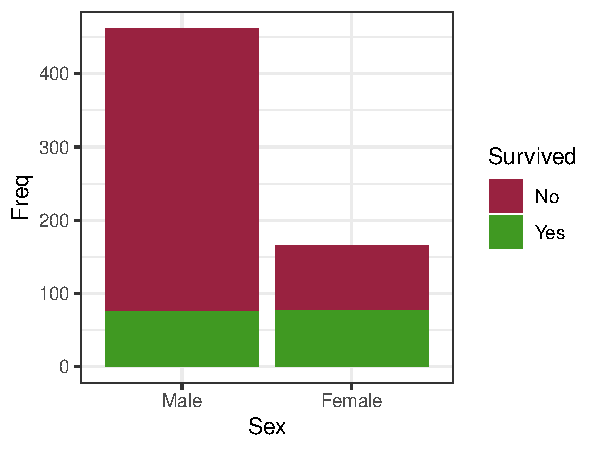
\includegraphics[width=\maxwidth]{figure/listings-unnamed-chunk-44-1} 

}

\begin{Sinput}
chisq.test(y_mat, correct = FALSE)
\end{Sinput}
\begin{Soutput}

	Pearson's Chi-squared test

data:  y_mat
X-squared = 59.159, df = 1, p-value = 1.454e-14
\end{Soutput}
\end{Schunk}
\begin{itemize}
	\item \textbf{Hypothesis}: \( H_0: p_{ij} = p_{i \bullet} p_{\bullet j} \) for \( i = 1,2 \) and \( j = 1,2 \) vs \( H_1: \) Not all equalities hold, or \( H_0: \) gender is independent of survival for adults in third class vs \( H_1: \)  gender and survival are not independent for adults in third class. 
	\item \textbf{Assumptions}: \( e_{ij} =y_{i \bullet} y_{\bullet j}/n \geq 5 \), do you think we have independent obs?
	\item \textbf{Test statistic}: \( T = \sum\limits_{i=1}^{2}\sum\limits_{j=1}^{2} \frac{(Y_{ij} - e_{ij})^2}{e_{ij}} \). Under \( H_0, T \sim \chi^2_1 \) approximately.
	\item \textbf{Observed test statistic}: \( t_0 = \sum\limits_{i=1}^{2} \sum\limits_{j=1}^{2} \frac{(y_{ij} - y_{i \bullet}y_{\bullet j}/n)^2}{y_{i \bullet}y_{\bullet j}/n} = 59.159 \).
	\item \textbf{P-value}: \( P(T\geq t_0) = P(\chi^2_1 \geq 59.159) < 0.001 \)
	\item \textbf{Decision}: We reject the null hypothesis that sex is independent of survival for adults in third class as the p-value is very small (much smaller than 0.05). Hence, there is evidence to suggest that survival status of passengers on the Titanic is related to the sex of the passenger.
\end{itemize}
\subsection{Testing for independence in general tables}
\subsubsection{Advertisement}
200 randomly sampled people are classified according to their income level and their reactions to an advertisement for a product (positive, negative, no opinion).
\begin{table}[H]
	\centering
	\begin{tabular}{@{}lccc|c@{}}
	\toprule
				& Positive & Negative & No Opinon & Total \\ \midrule
	High Income & 24       & 46       & 38        & 108   \\
	Low Income  & 32       & 22       & 38        & 92    \\ \midrule
	Total		& 56       & 68       & 76        & 200   \\ \bottomrule
	\end{tabular}
\end{table}
\subsubsection{General 2-Way contigency tables}
We now turn our attention from \( 2 \times 2 \) table to \( r \times c \) tables to \( r \times c \) tables with classifying factors \( R \) at \( r \) levels and \( S \) at \( c \) levels.\\
Let \( y_{ij} \) be the observed count in the \( (i,j) \)th cell. 
Summarise this in a contingency table,
\begin{table}[H]
	\centering
	\begin{tabular}{@{}ccccc|c@{}}
	\toprule
				 & \( S = 1 \)   		& \( S = 2 \)   	  & \( \dots \) & \( S = c \)  		  & Total		             \\ \midrule
	\( R = 1 \)  & \( y_{11} \) 		& \( y_{12} \) 		  & \( \dots \) & \( y_{1c} \)        & \( y_{1 \bullet} \)      \\
	\( R = 2 \)  & \( y_{21} \) 		& \( y_{22} \) 		  & \( \dots \) & \( y_{2c} \)        & \( y_{2 \bullet} \)      \\ 
	\( \vdots \) & \( \vdots \) 		& \( \vdots \) 		  &             & \( \vdots \)        & \( \vdots \) 	         \\ 
	\( R = r \)  & \( y_{r1} \) 		& \( y_{r2} \) 		  & \( \dots \) & \( y_{rc} \)        & \( y_{1 \bullet} \)      \\ \midrule
	Total 		 & \( y_{\bullet 1} \)  & \( y_{\bullet 2} \) & \( \dots \) & \( y_{\bullet c} \) & \( y_{\bullet\bullet} \) \\ \bottomrule
	\end{tabular}
\end{table}
\[
	y_{\bullet\bullet} = \sum_{i=1}^{r} \sum_{j=1}^{c} y_{ij} = n
\]
\subsubsection{Estimating \( p_{ij} \) under independence}
Suppose we have a completely random sample of size \( n \) classified by \( R \) and \( S \). We want to test \( H_0: R \) and \( S \) are independent.\\
If \( R \) and \( S \) are independent, by definition of independence,
\[
	p_{ij} = P(R = i, S = j) = P(R = i)P(S = j)
\]
We estimate the marginal probabilities \( P(R = i) \) and \( S = j \) via
\begin{itemize}
	\item \( (P = i) = p_{i \bullet} = \sum\limits_{j=1}^{c} p_{ij} \) estimated by \( \hat{p}_{i \bullet} = \frac{1}{n}\sum\limits_{j=1}^{c} y_{ij} = \frac{y_{i \bullet}}{n} \), and 
	\item \( (S = j) = p_{j \bullet} = \sum\limits_{i=1}^{r} p_{ij} \) estimated by \( \hat{p}_{\bullet j} = \frac{1}{n}\sum\limits_{i=1}^{r} y_{ij} = \frac{y_{\bullet j}}{n} \),
\end{itemize}
Under the independence hypothesis, the expected frequency in the  \( (i,j) \)th cell is
\[
	e_{ij} = n \hat{p}_{ij} = n \hat{p}_{i \bullet}\hat{p}_{\bullet j} = \frac{y_{i \bullet}y_{\bullet j}}{n}
\]
\subsubsection{Advertisement}
\begin{table}[H]
	\centering
	\begin{tabular}{@{}lccc|c@{}}
	\toprule
				 & Positive  		   & Negative             & No Opinon           & Row Total           \\ \midrule
	High Income  & \( p_{11} \)		   & \( p_{12} \) 	      & \( p_{13} \) 	    & \( p_{1 \bullet} \) \\
	Low Income   & \( p_{21} \) 	   & \( p_{22} \) 	      & \( p_{23} \) 	    & \( p_{2 \bullet} \) \\ \midrule
	Column Total & \( p_{\bullet 1} \) & \( p_{\bullet 2} \)  & \( p_{\bullet 3} \) & \( 1 \) 			  \\ \bottomrule
	\end{tabular}
\end{table}
Recall: \( X \) and \( Y \) are said to be independent if
\[
	P(X = x \mid Y = y) = P(X = x)P(Y = y)
\]
Let \( X \)  be a random variable representing opinion and let \( Y \) be a random variable representing income. Under independence,
\begin{align*}
	p_{12} &= P(X = \text{Negative}, Y = \text{High Income})\\
	       &= P(X = \text{Negative}) P(Y = \text{High Income})\\
		   &= p_{\bullet 2} p_{1 \bullet}
\end{align*}
\subsubsection{Test statistic}
Under \( H_0 \) of independence, the expected frequencies are \( e_{ij} = np_{ij} = np_{i \bullet}p_{\bullet j} \) for \( i = 1,2,\dotsc,r \) and \( j = 1,2,\dotsc,c \). Hence
\[
	T = \sum_{i=1}^{r}\sum_{j=1}^{c} \frac{(Y_{ij}-e_{ij})^2}{e_{ij}} = \sum_{i=1}^{r}\sum_{j=1}^{c} \frac{(Y_{ij}-np_{i \bullet}p_{\bullet j})^2}{np_{i \bullet}p_{\bullet j}}
\]
will be large if we should reject \( H_0 \).\\
However \( T \) includes unknown parameters \( p_{i \bullet} \) and \( p_{\bullet j} \). We estimate \( p_{i \bullet} \) and \( p_{\bullet j} \) with
\[
	\hat{p}_{i \bullet} = y_{i \bullet}/n \quad \hat{p}_{\bullet j} = y_{\bullet j}/n
\]
Hence, we may calculate the observed test statistic as
\[
	t_0 = \sum_{i=1}^{r}\sum_{j=1}^{c} \frac{(Y_{ij}-n \hat{p}_{i \bullet}\hat{p}_{\bullet j})^2}{n \hat{p}_{i \bullet}\hat{p}_{\bullet j}} = \sum_{i=1}^{r}\sum_{j=1}^{c}\frac{(y_{ij} - y_{i \bullet} y_{\bullet j}/n)^2}{y_{i \bullet}y_{\bullet j}/n}
\]
\subsubsection{Degrees of freedom}
\begin{table}[H]
	\centering
	\begin{tabular}{@{}lccc|c@{}}
	\toprule
				& Positive  	      & Negative		    & No Opinion		  & Total                     \\ \midrule
	High Income & \( y_{11} \)		  & \( y_{12} \) 	    & \( y_{13} \) 		  & \( y_{1 \bullet} = n_1 \) \\
	Low Income  & \( y_{21} \) 		  & \( y_{22} \) 	    & \( y_{23} \) 		  & \( y_{2 \bullet} = n_2 \) \\ \midrule
	Total       & \( y_{\bullet 1} \) & \( y_{\bullet 2} \) & \( y_{\bullet 3} \) & \( n \) 				  \\ \bottomrule
	\end{tabular}
\end{table}
\begin{itemize}
	\item The degrees of freedom for a \( r \times c \) table is \( (r-1)(c-1) \).
	\[
		(rc-1)-(r-1)-(c-1) = rc-r-c+1 = (r-1)(c-1)
	\]
	\item The degrees of freedom for a \( 2 \times 3 \) table is 2
\end{itemize}
\begin{redbox}{Workflow: Chi-squared Test of independence between two factors}
	\begin{itemize}
		\item \textbf{Hypothesis}: \( H_0: p_{ij} = p_{i \bullet} p_{\bullet j}, i = 1,2,\dotsc,r, j = 1,2,\dotsc,c \) vs \( H_1: \) Not all equalities hold. 
		\item \textbf{Assumptions}: Independent observations and  \( e_{ij} =y_{i \bullet} y_{\bullet j}/n \geq 5 \).
		\item \textbf{Test statistic}: \( T = \sum\limits_{i=1}^{r}\sum\limits_{j=1}^{c} \frac{(Y_{ij} - e_{ij})^2}{e_{ij}} \). Under \( H_0, T \sim \chi^2_{(r-1)(c-1)} \) approximately.
		\item \textbf{Observed test statistic}: \( t_0 = \sum_{i=1}^{r}\sum_{j=1}^{c}\frac{(y_{ij} - y_{i \bullet} y_{\bullet j}/n)^2}{y_{i \bullet}y_{\bullet j}/n} \).
		\item \textbf{P-value}: \( P(T\geq t_0) = P(\chi^2_{(r-1)(c-1)} \geq t_0) \)
		\item \textbf{Decision}: Reject \( H_0 \) if the p-value \( < \alpha \).
	\end{itemize}
\end{redbox}
As noted in the assumptions, this test should only really be applied when all cells have expected counts greater than 5, \( e_{ij} \geq 5 \). . If there are expected cell counts less than 5, consider using Fisher's exact test \( (2 \times 2) \) or simulation (general \( r \times c \) case).
\subsubsection{Advertisement}
200 randomly sampled people are classified according to their income level and their reactions to an advertisement for a product (positive, negative, no opinion).
\begin{table}[H]
	\centering
	\begin{tabular}{@{}lccc|c@{}}
	\toprule
				& Positive & Negative & No Opinon & Total \\ \midrule
	High Income & 24       & 46       & 38        & 108   \\
	Low Income  & 32       & 22       & 38        & 92    \\ \midrule
	Total		& 56       & 68       & 76        & 200   \\ \bottomrule
	\end{tabular}
\end{table}
The test for independence between factors of \textit{income level} and \textit{opinion} is
\begin{itemize}
	\item \textbf{Hypothesis}: \( H_0: p_{ij} = p_{i \bullet} p_{\bullet j}, i = 1,2, j = 1,2,e \) vs \( H_1: \) Not all equalities hold \textbf{or} \( H_0: \) income level is independent of opinion vs \( H_1 \):  income level is not independent of opinion. 
	\item \textbf{Assumptions}: independent observations (satisfied, they were randomly sampled) \( e_{ij} =y_{i \bullet} y_{\bullet j}/n \geq 5 \)  (satisfied, checked with calculations).
	\item \textbf{Test statistic}: \( T = \sum\limits_{i=1}^{r}\sum\limits_{j=1}^{c} \frac{(Y_{ij} - e_{ij})^2}{e_{ij}} \). Under \( H_0, T \sim \chi^2_2 \) approximately.
	\item \textbf{Observed test statistic}: \( t_0 = \sum_{i=1}^{r}\sum_{j=1}^{c}\frac{(y_{ij} - y_{i \bullet} y_{\bullet j}/n)^2}{y_{i \bullet}y_{\bullet j}/n} = 8.39 \).
	\item \textbf{P-value}: \( P(T\geq t_0) = P(\chi^2_2 \geq 8.39) = 0.015 \)
	\item \textbf{Decision}: Since the p-value is less than 0.05, the data provide evidence against \( H_0 \). There is evidence to suggest that there is an association between income level and opinion.
\end{itemize}
\begin{Schunk}
\begin{Sinput}
y = c(24,32,46,22,38,38)
n = sum(y)
c = 3
r = 2
y_mat = matrix(y, nrow = r, ncol = c)
colnames(y_mat) = c("Positive", "Negative", "No opinion")
rownames(y_mat) = c("High income", "Low income")
y_mat
\end{Sinput}
\begin{Soutput}
            Positive Negative No opinion
High income       24       46         38
Low income        32       22         38
\end{Soutput}
\begin{Sinput}
chisq.test(y_mat, correct = FALSE)
\end{Sinput}
\begin{Soutput}

	Pearson's Chi-squared test

data:  y_mat
X-squared = 8.3871, df = 2, p-value = 0.01509
\end{Soutput}
\end{Schunk}
\section{Testing in small samples}\label{sec:9}
\subsection{Fisher's exact test}
\subsubsection{Lady tasting tea}
Given a cup of tea with milk, a lady claims she can discriminate as to whether milk or tea was first added to the cup.
\begin{greenbox}
	\textbf{How could we test this claim? What information would we need?}
\end{greenbox}
Fisher proposed preparing 8 cups of tea
\begin{itemize}
	\item 4 cups where tea was added before milk
	\item 4 cups where milk was added before tea
\end{itemize}
The lady would then be randomly given the cups of tea and asked to identify the 4 where tea was added before milk.\\
We would need to record:
\begin{itemize}
	\item Which cups had tea or milk added first (\textbf{truth}).
	\item Which cups the lady claimed had tea or milk added first (\textbf{predicted}).
\end{itemize}
\begin{Schunk}
\begin{Sinput}
truth = c("milk", "tea", "tea", "milk", "tea", "tea", "milk", "milk")
predicted = c("milk", "tea", "tea", "milk", "tea", "tea", "milk", "milk")
tea_mat = table(truth, predicted)
tea_mat
\end{Sinput}
\begin{Soutput}
      predicted
truth  milk tea
  milk    4   0
  tea     0   4
\end{Soutput}
\begin{Sinput}
chisq.test(tea_mat, correct = FALSE)
\end{Sinput}
\begin{Soutput}

	Pearson's Chi-squared test

data:  tea_mat
X-squared = 8, df = 1, p-value = 0.004678
\end{Soutput}
\end{Schunk}
\subsubsection{Fisher's exact test}
\begin{itemize}
	\item The \( \chi^2 \) approximation for the test statistic is only reasonable when \( n \) is sufficiently large.
	\item I.e. we need the expected cell frequencies to all be 5 or more.
	\item If this is not the case, then we need to take care and maybe consider \textbf{exact} tests, i.e. calculating the exact p-value for the test statistic.
	\item All that we really need to assume is that we have independent observations (and we condition on knowing the row and column totals).
	\item In R the function \lstinline|fisher.test()|  is available to carry out these calculations both for \( 2 \times 2 \) tables and general contingency tables.
\end{itemize}
\subsubsection{Formulating the null hypothesis}
The simplest exact test for contingency tables is Fisher's test for \( 2 \times 2 \) tables.
Consider the table:
\begin{table}[H]
	\centering
	\begin{tabular}{@{}c|cc|c@{}}
	\toprule
				   & \( A_1 \)          & \( A_2 \)          & \textbf{Total}     \\ \midrule
	\( B_1 \)      & \( y_{11} \)       & \( y_{12} \)       & \( y_{1\bullet} \) \\
	\( B_2 \)      & \( y_{21} \)       & \( y_{12} \)       & \( y_{2\bullet} \) \\ \midrule
	\textbf{Total} & \( y_{\bullet1} \) & \( y_{\bullet2} \) & \( n \)            \\ \bottomrule
	\end{tabular}
\end{table}
Let \( \theta \) be the \textcolor{myred}{odds ratio}.\\
Fisher's exact test can be thought of as testing the null hypothesis,
\[
	H_0: \theta = 1
\]
against the alternative \( H_1: \theta > 1 \) or \( H_1: \theta < 1 \) or \( H_1: \theta \neq 1 \).\\
The test is based on the observed value of \( y_{11} \) given the marginal totals.\\
The \textbf{test statistic} is \( Y_{11} \) and the \textbf{observed test statistic} is \( y_{11} \).
\subsubsection{The hypergeometric distrubution}
For a \( 2 \times 2 \) if we know the row and column and \( y_{11} \) then the table is completely specified.\\
If \( H_0 \) is true and we know the \( y_{1\bullet}, y_{\bullet1} \) and \( n \) values we expect \( y_{\bullet1} \times \frac{y_{1\bullet}}{n} \) in the \( (1,1) \)th cell.\\
To obtain the distribution of \( y_{11} \) given the marginal values we note that this is like selecting \( y_{1\bullet} \) values from \( n \) where \( y_{1\bullet} \) and ype \( B_1 \) and \( y_{2\bullet} \) are type \( B_2 \).\\
This motivates the use of the hypergeometric distribution:
\[
	P(Y_{11} = y_{11}) = \frac{\binom{y_{1 \bullet}}{y_{11}}\binom{y_{2 \bullet}}{y_{\bullet 1} - y_{11}}}{\binom{n}{y_{\bullet 1}}}e.
\]
\subsubsection{p-values}
To calculate the p-value for a particular table we need to:
\begin{itemize}
	\item enumerate all tables, as extreme, or more extreme than the observed table \textbf{with the same marginal totals}; and
	\item sum up the probability of each of these tables.
\end{itemize}
\subsubsection{Lady tasting tea}
\begin{Schunk}
\begin{Sinput}
truth = c("milk", "tea", "tea", "milk", "tea", "tea", "milk", "milk")
predicted = c("milk", "tea", "tea", "milk", "tea", "tea", "milk", "milk")
tea_mat = table(truth, predicted)
tea_mat
\end{Sinput}
\begin{Soutput}
      predicted
truth  milk tea
  milk    4   0
  tea     0   4
\end{Soutput}
\end{Schunk}
For Fisher's exact test we:
\begin{enumerate}
	\item Consider all possible permutations of the  \( 2 \times 2 \) contingency table with the same \textit{marginal totals} (in this case \( y_{i\bullet} = y_{\bullet j} = 4 \)).
	\item Calculate how many of these were equal to or`` more extreme'' than what we observed.
\end{enumerate}
\begin{table}[H]
	\centering
	\begin{tabular}{@{}c|cc|c@{}}
	\toprule
				   & \multicolumn{2}{c|}{Predicted}                  & \\
	Truth          & Milk                   & Tea                    & \textbf{Total}                   \\ \midrule
	Milk           & 4                      & 0                      & \( y_{1\bullet} = 4 \)           \\
	Tea            & 0                      & 4                      & \( y_{2\bullet} = 4 \)           \\ \midrule
	\textbf{Total} & \( y_{\bullet1} = 4 \) & \( y_{\bullet2} = 4 \) & \( y_{\bullet\bullet} = n = 8 \) \\ \bottomrule
	\end{tabular}
\end{table}
\subsubsection{How do we define more extreme?}
Let us define a test statistic
\begin{center}
	T = number of cups of tea before milk that she got correct.
\end{center}
This test statistic has 5 outcomes: \( \{0,1,2,3,4\} \).\\
Given that there are 8 cups of tea, there are \( \binom{8}{4} = 70 \) ways that we could predict which cups had tea added before milk.\\
We can look at all 70 ways and calculate how often we see a test statistic of \( 0,1,2,3 \) or 4.
\begin{table}[H]
	\begin{tabular}{@{}l|ccccc|c@{}}
	Number correct: \( t_i \)            & 0 								  & 1                                   & 2                                  & 3 & 4 &  \\ \midrule
	How many ways:  \( f_i \)            & \( \binom{4}{0}\binom{4}{4} = 1 \) & \( \binom{4}{1}\binom{4}{3} = 16 \) & \( \binom{4}{2}\binom{4}{2} =36 \) & \( \binom{4}{3}\binom{4}{1} = 16 \) &  \( \binom{4}{4}\binom{4}{0} = 1 \) & 70 \\
	Corresponding probability: \( p_i \) & \( \frac{1}{70} \)                 & \( \frac{16}{70} \)                 & \( \frac{36}{70} \)                & \(\frac{16}{70} \) & \( \frac{1}{70} \) & 1 \\ \bottomrule
	\end{tabular}
\end{table}
\( P(\text{Getting at least 4 correct}) = P(T = 4) = \frac{1}{70} = 0.014 \) 
\begin{Schunk}
\begin{Sinput}
fisher.test(tea_mat)
\end{Sinput}
\begin{Soutput}

	Fisher's Exact Test for Count Data

data:  tea_mat
p-value = 0.02857
alternative hypothesis: true odds ratio is not equal to 1
95 percent confidence interval:
 1.339059      Inf
sample estimates:
odds ratio 
       Inf 
\end{Soutput}
\begin{Sinput}
fisher.test(tea_mat, alternative = "greater") # correct in this setting
\end{Sinput}
\begin{Soutput}

	Fisher's Exact Test for Count Data

data:  tea_mat
p-value = 0.01429
alternative hypothesis: true odds ratio is greater than 1
95 percent confidence interval:
 2.003768      Inf
sample estimates:
odds ratio 
       Inf 
\end{Soutput}
\end{Schunk}
\subsubsection{Cancer of the larynx}
Mendenhall et al. (1984) report the results of a study comparing radiation therapy with surgery in treating cancer of the larynx.
\begin{table}[H]
	\centering
	\begin{tabular}{@{}c|cc|c@{}}
	\toprule
				      & \textbf{Cancer controlled} & \textbf{Cancer bot controlled} & \textbf{Total} \\ \midrule
	Surgery           & 21                         & 2                              & 23             \\
	Radiation therapy & 15                         & 3                              & 18             \\ \midrule
	Total             & 36                         & 5                              & 41             \\ \bottomrule
	\end{tabular}
\end{table}
Suppose that we wish to test \( H_0: \theta =1 \) (both treatments equally effective) against \( H_1: \theta >1 \) (surgery more effective).\\
First we need to enumerate all tables which are \textcolor{mygreen}{as extreme} or \textcolor{myred}{more extreme} than the observed table. These are:\\
The original table:
\begin{table}[H]
	\centering
	\begin{tabular}{@{}c|cc|c@{}}
	\toprule
				      & \textbf{Cancer controlled} & \textbf{Cancer bot controlled} & \textbf{Total} \\ \midrule
	Surgery           & \textcolor{mygreen}{21}    & 2                              & \textbf{23}    \\
	Radiation therapy & 15                         & 3                              & \textbf{18}    \\ \midrule
	\textbf{Total}    & \textbf{36}                & \textbf{5}                     & \textbf{41}    \\ \bottomrule
	\end{tabular}
\end{table}
And the tables where surgery controlled more than \textcolor{mygreen}{21} (i.e. \textcolor{myred}{22} or \textcolor{myred}{23}) patients, holding the \textbf{margins} constant.
\begin{table}[H]
	\centering
	\begin{tabular}{@{}c|cc|c@{}}
	\toprule
				      & \textbf{Cancer controlled} & \textbf{Cancer bot controlled} & \textbf{Total} \\ \midrule
	Surgery           & \textcolor{myred}{22}      & 1                              & \textbf{23}    \\
	Radiation therapy & 15                         & 3                              & \textbf{18}    \\ \midrule
	\textbf{Total}    & \textbf{36}                & \textbf{5}                     & \textbf{41}    \\ \bottomrule
	\end{tabular}
\end{table}
\begin{table}[H]
	\centering
	\begin{tabular}{@{}c|cc|c@{}}
	\toprule
				      & \textbf{Cancer controlled} & \textbf{Cancer bot controlled} & \textbf{Total} \\ \midrule
	Surgery           & \textcolor{myred}{23}      & 0                              & \textbf{23}    \\
	Radiation therapy & 15                         & 3                              & \textbf{18}    \\ \midrule
	\textbf{Total}    & \textbf{36}                & \textbf{5}                     & \textbf{41}    \\ \bottomrule
	\end{tabular}
\end{table}
Let \( X \) be the number of surgery cases where cancer is controlled. Applying Fisher's approach
\begin{align*}
	\text{p-value}  
	&= P (X \geq 21 \mid \text{marginal totals} )\\
	&= P (X = 21, 22, 23 \mid \text{marginal totals} )\\
	&= P (X = 21 \mid \text{marginal totals} ) \\
	  & \qquad {} + P (X = 22 \mid \text{marginal totals} )\\
	  & \qquad {} + P (X = 23 \mid \text{marginal totals} )\\
	&= \frac{\binom{23}{21} \binom{18}{15}}{\binom{41}{36}} + \frac{\binom{23}{22} \binom{18}{14}}{\binom{41}{36}} + \frac{\binom{23}{23} \binom{18}{13}}{\binom{41}{36}} + \\
	&=  0.3808.
\end{align*}
\begin{Schunk}
\begin{Sinput}
y_mat = matrix(c(21, 15, 2, 3), ncol = 2)
colnames(y_mat) = c("Controlled", "Not controlled")
rownames(y_mat) = c("Surgery", "Radiation therapy")
y_mat
\end{Sinput}
\begin{Soutput}
                  Controlled Not controlled
Surgery                   21              2
Radiation therapy         15              3
\end{Soutput}
\begin{Sinput}
fisher.test(y_mat, alternative = "greater")
\end{Sinput}
\begin{Soutput}

	Fisher's Exact Test for Count Data

data:  y_mat
p-value = 0.3808
alternative hypothesis: true odds ratio is greater than 1
95 percent confidence interval:
 0.2864828       Inf
sample estimates:
odds ratio 
  2.061731 
\end{Soutput}
\end{Schunk}
\subsubsection{Drawbacks}
Why don't we use Fisher's exact test all the time?
\begin{itemize}
	\item The calculation of the p-value requires conditioning on row and column margins being fixed.
	\item Computationally difficult for large samples.
	\item It can be generalized to \( r \times c \) two-way contingency tables but is very difficult to compute. Generally requires use of Monte Carlo (i.e. random permutation).
\end{itemize}
\begin{table}[H]
	\centering
	\begin{tabular}{@{}c|ccc|c@{}}
	\toprule
	\( X \; Y \) 	   & \( y_1 \)   & \( y_2 \)   & \( y_3 \)   & \textbf{Row total}    \\ \midrule
	\( x_1 \)          & \( a \)     & \( b \)     & \( c \)     & \( a + b + c \)       \\
	\( x_2 \)          & \( d \)     & \( e \)     & \( f \)     & \( d + e + f \)       \\ \midrule
	\textbf{Row total} & \( a + d \) & \( b + e \) & \( c + f \) & \( n = a+b+c+d+e+f \) \\ \bottomrule
	\end{tabular}
\end{table}
\subsection{Yates' chi-squared test}
\subsubsection{Yates' Corrected \( \chi^2 \) Test}
Yates (1934) modified the standard chi-squared test with a continuity correction. It is usually more accurate when counts in each cell are small. Yates' statistic for \( 2 \times 2 \) tables is:
\[
	T = \sum_{i=1}^2\sum_{j=1}^2 \frac{(\lvert Y_{ij} - e_{ij} \rvert - 0.5)^2}{e_{ij}}
\]
which approximately follows a \( \chi^2_1 \) distribution under \( H_0 \).\\
\textbf{Logic behind continuity corrections}
In general, if we have an \textit{integer-valued random variable} \( X \) which we would like to approximate with a continuous random variable \( Y \) then
\[
	P(X \leq x) \approx P(Y \leq x + 0.5) \quad \text{and} \quad P(X \geq x) \approx P(Y \geq x - 0.5).
\]
\begin{Schunk}
\begin{Sinput}
chisq.test(tea_mat, correct = TRUE)
\end{Sinput}
\begin{Soutput}
Warning in stats::chisq.test(x, y, ...): Chi-squared approximation may be incorrect
\end{Soutput}
\begin{Soutput}

	Pearson's Chi-squared test with Yates' continuity correction

data:  tea_mat
X-squared = 4.5, df = 1, p-value = 0.03389
\end{Soutput}
\end{Schunk}
\subsection{Permutation testing}
\subsubsection{Fingerprints}
The study of Galton (1892) marked one of the first formal statistical examinations of association for contingency tables. His work involved determining the association of fingerprint characteristics of 105 fraternal (or dizygotic) male twins. One male twin was ``earmarked'' as twin A and his brother was ``earmarked'' as twin B. For each twin, the number of Arches, Loops and Whorls was counted and summarised in the \( 3 \times 3 \) contigency table of Galton (1892, Table XXII, pg. 175).
\begin{figure}[H]
	\centering
	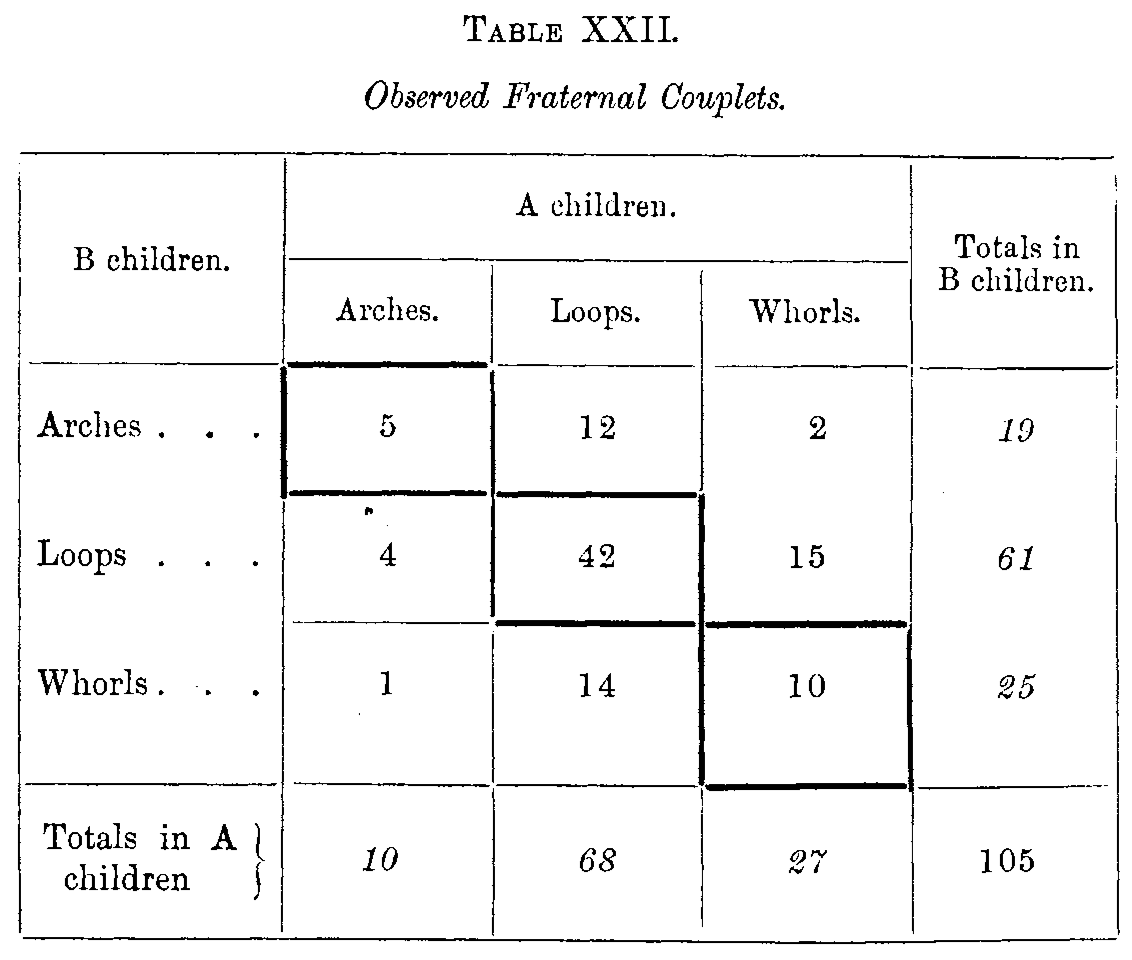
\includegraphics[scale=0.5]{fingerprints}
\end{figure}
\begin{Schunk}
\begin{Sinput}
galton.dat <- matrix(c(5, 4, 1, 12, 42, 14, 2, 15, 10), 3, 3)
rownames(galton.dat) = c("Arches-B", "Loops-B", "Whorls-B")
colnames(galton.dat) = c("Arches-A", "Loops-A", "Whorls-A")
galton.dat
\end{Sinput}
\begin{Soutput}
         Arches-A Loops-A Whorls-A
Arches-B        5      12        2
Loops-B         4      42       15
Whorls-B        1      14       10
\end{Soutput}
\begin{Sinput}
chisq.test(galton.dat)
\end{Sinput}
\begin{Soutput}
Warning in stats::chisq.test(x, y, ...): Chi-squared approximation may be incorrect
\end{Soutput}
\begin{Soutput}

	Pearson's Chi-squared test

data:  galton.dat
X-squared = 11.17, df = 4, p-value = 0.02472
\end{Soutput}
\end{Schunk}
\subsubsection{Monte Carlo simulation}
The \textbf{Monte Carlo simulation procedure} is as follows:
\begin{itemize}
	\item Analyse the sample as one would normally do in a hypothesis test (up to, and including, the calculation of the test statistic)
	\item From the original sample being analysed, resample it LOTS of times
	\item The test statistic of interest is calculated for each of the resamples (so that we have the sampling distribution of the test statistic)
	\item This leads to LOTS of test statistics that will be used to calculate p-values for the observed statistic.
\end{itemize}
Monte Carlo p-values are calculated by determining the proportion of the resampled test statistics as or more extrame than the observed test statistic.
\textbf{No assumptions} are made about the underlying distribution of the population.
\subsubsection{Fingerprints}
Monte Carlo p-values may be obtained by randomly generating contingency tables given that the margins are assumed fixed.\\
To randomly generate a contingency table with the same margins as the original table we use the \lstinline|r2dtable()| function in R.\\
\lstinline|r2dtable()| generates a \textbf{list} of random 2-way tables given marginals.
\begin{Schunk}
\begin{Sinput}
row_totals = rowSums(galton.dat)
col_totals = colSums(galton.dat)
B = 10000
set.seed(123)
x_list = r2dtable(n = B, 
                  r = row_totals,
                  c = col_totals)
x_list[[1]]
\end{Sinput}
\begin{Soutput}
     [,1] [,2] [,3]
[1,]    2   10    7
[2,]    7   43   11
[3,]    1   15    9
\end{Soutput}
\begin{Sinput}
chisq.test(x_list[[1]])
\end{Sinput}
\begin{Soutput}
Warning in stats::chisq.test(x, y, ...): Chi-squared approximation may be incorrect
\end{Soutput}
\begin{Soutput}

	Pearson's Chi-squared test

data:  x_list[[1]]
X-squared = 5.2367, df = 4, p-value = 0.2639
\end{Soutput}
\end{Schunk}
The observed test statistic for the first random sample is 5.24.\\
For each of the 10,000 randomly generated contingency tables, we can record their test statistic then determine what proportion of them are equal to (or exceed) the observed test statistic.
\begin{Schunk}
\begin{Sinput}
rnd.chisq = numeric(B) # initialise an empty vector
for (i in 1:B){ # loop over B iterations
  # each time save the test statistic
  rnd.chisq[i] = chisq.test(x_list[[i]])$statistic
}
# what proportion of times did we observe a test statistic
# as or more extreme than what we observed?
sum(rnd.chisq >= 11.1699)/B
\end{Sinput}
\begin{Soutput}
[1] 0.022
\end{Soutput}
\end{Schunk}
Here, the Monte Carlo p-value is 0.022 (comparable to theoretical p-value of 0.0247).
\begin{Schunk}
\begin{Sinput}
par(cex = 0.6)
hist(rnd.chisq)
abline(v = 11.1699, col = "#224099", lwd = 2)
axis(1, 11.1699, col.axis = "#224099")
\end{Sinput}


{\centering 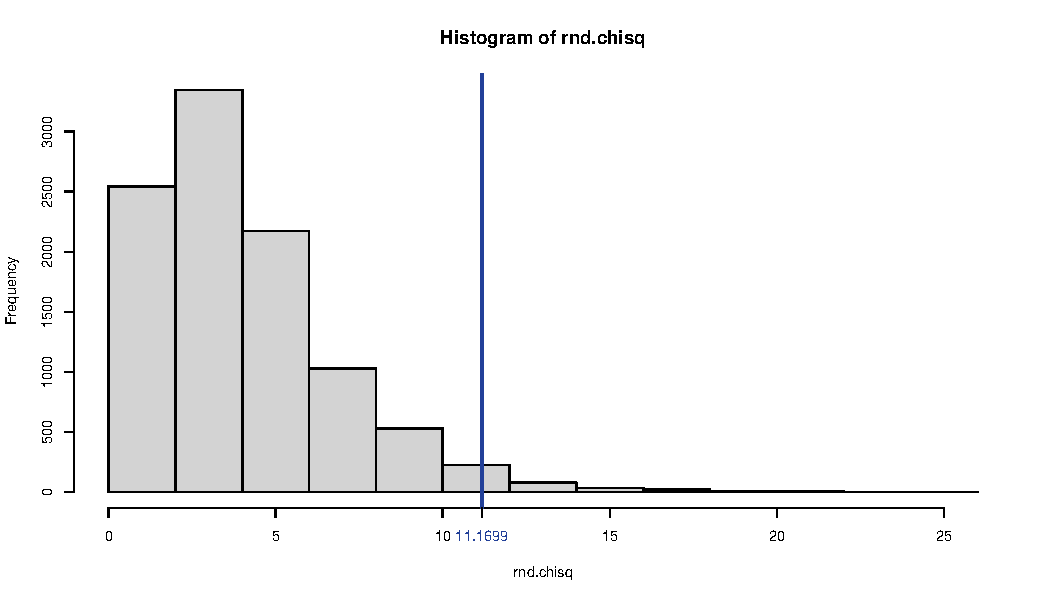
\includegraphics[width=\maxwidth]{figure/listings-unnamed-chunk-54-1} 

}

\end{Schunk}
\lstinline|chisq.test(..., simulate.p.value = TRUE)| calculates Monte Carlo p-values and does so using \lstinline|r2dtable()| internally.
\begin{Schunk}
\begin{Sinput}
chisq.test(galton.dat, simulate.p.value = TRUE)
\end{Sinput}
\begin{Soutput}

	Pearson's Chi-squared test with simulated p-value (based on 2000
	replicates)

data:  galton.dat
X-squared = 11.17, df = NA, p-value = 0.01999
\end{Soutput}
\end{Schunk}
The default is 2000 contingency tables. We could use 10,000 resamples by specifying \lstinline|B = 10000|.
\begin{Schunk}
\begin{Sinput}
chisq.test(galton.dat, simulate.p.value = TRUE, B = 10000)
\end{Sinput}
\begin{Soutput}

	Pearson's Chi-squared test with simulated p-value (based on 10000
	replicates)

data:  galton.dat
X-squared = 11.17, df = NA, p-value = 0.0232
\end{Soutput}
\end{Schunk}

\section{Testing Means}\label{sec:10}
\subsection{General \( t \)-test background}
\subsubsection{What is it?}
Some basic probability facts about samples from \textit{normal populations} will prove useful.
\begin{enumerate}
	\item The sample mean from a normal sample is itself normally distributed.
	\item The sample variance from a normal sample has a \textit{scaled} \( \chi^2 \) distribution.
	\item The sample mean and sample variance from a normal sample are \textit{statistically independent}.
	\item If \( Z \sim \mathcal{N}(0,1) \) is independent of a \( \chi^2_d \) random variable, the quantity
	\[
		\frac{Z}{\sqrt{\chi^2_d}/d} \sim t_d,
	\]
	a \( t \)-distribution with \( d \) degrees of freedom.
\end{enumerate}
\subsubsection{The \( t \)-statistic}
\begin{itemize}
	\item Given a population mean \( \mu \), the sample mean and variance \( \overline{X} \) and \( S^2 \), the ratio
	\[
		\frac{\overline{X}-\mu}{S / \sqrt{n}} = \frac{\sqrt{n}(\overline{X} - \mu)/\sigma}{S / \sigma} \sim t_{n-1}.
	\]
	\begin{itemize}
		\item the numerator is \( \mathcal{N}(0,1) \);
		\item the denominator is \( \sqrt{\chi^2_{N-1}/n-1} \), independent of the numerator.
	\end{itemize}
	\item In many statistical applications we have a model whereby a certain statistic has this general form:
	\begin{itemize}
		\item some estimator of some parameter is normally distributed;
		\item a standard error based on the data has a distribution like \( \sqrt{\chi^2_d/d} \) times the true SD of the estimator (for some \( d \)) and is \textit{independent} of the estimator;
		\item then the ratio \( \frac{\text{estimator}-\text{true value}}{\text{standard error}} \sim t_d \).
	\end{itemize}
\end{itemize}
\subsection{One sample \( t \)-test}
\subsubsection{Beer contents}
Beer contents in a pack of six bottles (in millilitres) are:
\begin{Schunk}
\begin{Sinput}
y = c(374.8, 375.0, 375.3, 374.8, 374.4, 374.9)
\end{Sinput}
\end{Schunk}
Is the mean beer content less than the 375 ml claimed on the label?
\begin{Schunk}
\begin{Sinput}
library("ggplot2")
df = data.frame(y)
set.seed(88)
ggplot(df, aes(x = "", y = y)) +
  geom_boxplot(alpha = 0.5, coef = 10) + 
  geom_dotplot(binaxis = 'y', stackdir = 'center') + 
  geom_hline(yintercept = 375, colour = "#224099", linetype = "dashed") + 
  labs(y = "Beer volume (ml)", x = "") +
  theme_bw() + 
  theme(axis.ticks.x = element_blank(), axis.text.x = element_blank())
\end{Sinput}


{\centering 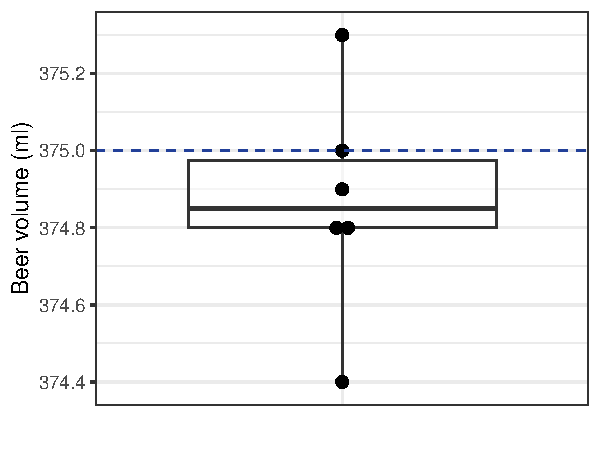
\includegraphics[width=\maxwidth]{figure/listings-unnamed-chunk-58-1} 

}

\end{Schunk}
\subsubsection{Hypothesis testing}
\begin{redbox}{Workflow: General hypothesis test}
	\begin{itemize}
		\item \textbf{Hypotheses}: \( H_0: \theta = \theta_0 \) vs \( H_1: \theta > \theta_0 \) or \( \theta < \theta_0 \) or \( \theta \neq \theta_0 \)
		\item \textbf{Assumptions}: \( X_1,X_2,\dotsb,X_n \sim F_\theta \)
		\item \textbf{Test Statistic}: \( T = f(X_1,X_2,\dotsb,X_n) \)  
		\item \textbf{Observed Test Statistic}: \( t_0 = f(x_1,x_2,\dotsc,x_n) \).
		\item \textbf{Significance}: p-value = \( P(T \geq t_0) \) or \( P(T \leq t_0) \) or \( 2P(T \geq \lvert t_0 \rvert) \)
		\item \textbf{Decision}:  If the p-value is less than \( \alpha \), there is ecidence against \( H_0 \).
	\end{itemize}
\end{redbox}
\subsubsection{Hypothesis}
\begin{itemize}
	\item The statement against which you search for evidence is called the null hypothesis, and is denoted by \( H_0 \). It is generally a ``no difference'' statement.
	\item The statement you claim is called the alternative hypothesis, and is denoted by \( H_1 \).
\end{itemize}
\[
	H_0: \theta = \theta_0 \quad\text{vs}\quad
	\begin{cases}
		H_1: \theta > \theta_0 &\text{(upper-side alternative)} \\
		H_1: \theta < \theta_0 &\text{(lower-side alternative)} \\
		H_1: \theta \neq \theta_0 &\text{(two-sided alternative)} \\
	\end{cases}
\]
\subsubsection{Assumptions}
\begin{itemize}
	\item Each observation \( X_1,X_2,\dotsc,X_n \) is chosen at random from a population.
	\item We say that such random variables are \textit{idd} (independently and identically distributed).
	\item Each test we consider will have its own assumptions.
\end{itemize}
\subsubsection{Test statistic}
\begin{itemize}
	\item Since observations \( X_i \) vary from sample to sample we can never be sure whether \( H_0 \) is true or not.
	\item We use a test statistic \( T = f(X_1,\dotsc,X_n) \) to test if the data are consistent with \( H_0 \) such that the distribution of \( T \) is known assuming \( H_0 \) is true.
\end{itemize}
The \textbf{observed test statistic}, \( t_0 \), is where we plug our observed data into the formula for the test statistic.\\
Large (positive or negative depending on \( H_1 \)) observed test statistic values is taken as evidence of poor agreement with \( H_0 \)
\subsubsection{Significance}
The p-value is defined as the probability of getting a test statistic, \( T \), \textit{as or more extreme} than the value we observed, \( t_0 \), \textit{assuming} that \( H_0 \) is true.\\
Typical p-value statements:
\begin{itemize}
	\item For \( H_1: \theta > \theta_0 \), p-value \( = P(T \geq t_0) \) 
	\item For \( H_1: \theta < \theta_0 \), p-value \( = P(T \leq -t_0) \) 
	\item For \( H_1: \theta \neq \theta_0 \), p-value \( = 2P(T \geq \lvert t_0 \rvert) \) 
\end{itemize}
\subsubsection{Decision}
An observed \textit{large} positive or negative value of \( t_0 \) and hence small p-value is taken as evidence of poor agreement with \( H_0 \).
\begin{itemize}
	\item If the p-value is small, then either \( H_0 \) is true and the poor agreement is due to an unlikely event, or \( H_0 \) is false. Therefore\dots
	\item the smaller the p-value, the stronger the evidence against \( H_0 \) in favour of \( H_1 \).
	\item A large p-value does not mean that there is evidence that \( H_0 \) is true
	\item The level of significance, \( \alpha \), is the strength of evidence needed to reject \( H_0 \) (often \( \alpha = 0.05 \))
\end{itemize}
\subsubsection{One sample \( t \)-test}
Suppose we have a sample \( X_1,X_2,\dotsc,X_n \) of size \( n \) drawn from a normal population with an unknown variance \( \sigma^2 \). Let \( x_1,x_2,\dotsc,x_n \) be the \textcolor{myred}{observed values}. We want to test the population mean \( \mu \).  
\begin{redbox}{Workflow: One Sample \( t \)-test}
	\begin{itemize}
		\item \textbf{Hypotheses}: \( H_0: \mu = \mu \) vs \( H_1: \mu > \mu_0, \mu < \mu_0 \) or \( \mu \neq \mu_0 \)
		\item \textbf{Assumptions}: \( X_i \) are iid random variables and follow \( \mathcal{N} (\mu,\sigma^2) \) 
		\item \textbf{Test Statistic}: \( T = \frac{\overline{X} - \mu_0}{S / \sqrt{n}} \). Under \( H_0, T \sim t_{n-1} \)   
		\item \textbf{Observed Test Statistic}: \( t_0 = \frac{\overline{x} - \mu_0}{s / \sqrt{n}} \).
		\item \textbf{p-value}: \( P(t_{n-1} \geq t_0) \) or \( P(t_{n-1} \leq t_0) \) or \( 2P(t_{n-1} \geq \lvert t_0 \rvert) \)
		\item \textbf{Decision}: Reject \( H_0 \) in favor of \( H_1 \) if the p-value is less then \( \alpha \).
	\end{itemize}
\end{redbox}
\subsubsection{Beer contents}
Beer contents in a pack of six bottles (in millilitres) are:
\[
	374.8, 375.0, 375.3, 374.8, 374.4, 374.9
\]
Is the mean beer content less than the 375 ml claimed on the label?
\begin{Schunk}
\begin{Sinput}
x = c(374.8, 375.0, 375.3, 374.8, 374.4, 374.9)
mean(x)
\end{Sinput}
\begin{Soutput}
[1] 374.8667
\end{Soutput}
\begin{Sinput}
sd(x)
\end{Sinput}
\begin{Soutput}
[1] 0.294392
\end{Soutput}
\end{Schunk}
\begin{itemize}
	\item \textbf{Hypotheses}: \( H_0: \mu = 375 \) vs \( H_1: \mu < 375 \)
	\item \textbf{Assumptions}: \( X_i \) are iid random variables and follow \( \mathcal{N} (\mu,\sigma^2) \) 
	\item \textbf{Test Statistic}: \( T = \frac{\overline{X} - \mu_0}{S / \sqrt{n}} \). Under \( H_0, T \sim t_{n-1} \)   
	\item \textbf{Observed Test Statistic}: \( t_0 = \frac{375.87 - 375}{0.29 / \sqrt{6}} = -1.11 \).
	\item \textbf{p-value}: \( P(t_5 \leq -1.11) = 0.16 \)
	\item \textbf{Decision}: The data is consistent with the null hypothesis \( H_0 \).
\end{itemize}
\begin{Schunk}
\begin{Sinput}
t.test(x, mu = 375, alternative = "less")
\end{Sinput}
\begin{Soutput}

	One Sample t-test

data:  x
t = -1.1094, df = 5, p-value = 0.1589
alternative hypothesis: true mean is less than 375
95 percent confidence interval:
     -Inf 375.1088
sample estimates:
mean of x 
 374.8667 
\end{Soutput}
\end{Schunk}
\subsection{Two sample \( t \)-test}
\subsubsection{What if you have two samples?}
There are times that we want to test if the population means of two samples are different.\\
Here we are left with two possible scenarios
\begin{itemize}
	\item Two independent samples
	\item Two related samples (dependent samples or repeated measures)
\end{itemize}
\subsubsection{Smokers and blood platelet aggregation}
Blood samples are taken from 11 smokers and 11 non-smokers to measure aggregation of blood platelets.
\begin{Schunk}
\begin{Sinput}
non_smokers = c(25, 25, 27, 44, 30, 67, 53, 53, 52, 60, 28)
smokers =  c(27, 29, 37, 36, 46, 82, 57, 80, 61, 59, 43)
dat = data.frame(
  platelets = c(non_smokers, smokers),
  status = c(rep("Non smokers", length(non_smokers)), 
  rep("Smokers", length(smokers)))
)
library(dplyr)
sum = dat |>
  group_by(status) |>
  	summarise(Mean = mean(platelets),
  	SD = sd(platelets), 
  	n = n())
knitr::kable(sum, digits = 1, booktabs=TRUE) |>
  kable_styling(position="center", latex_options = "hold_position")
\end{Sinput}
\begin{table}[!h]
\centering
\begin{tabular}{lrrr}
\toprule
status & Mean & SD & n\\
\midrule
Non smokers & 42.2 & 15.6 & 11\\
Smokers & 50.6 & 18.9 & 11\\
\bottomrule
\end{tabular}
\end{table}

\end{Schunk}
\subsubsection{Visualising Blood Platelet Aggregation}
Is the aggregation of blood platelets affected by smoking?
\begin{Schunk}
\begin{Sinput}
library(ggplot2)
ggplot(dat) + aes(x = status, y = platelets) +
  geom_boxplot() + 
  geom_jitter(width = 0.15, colour = "#224099") + 
  labs(x = "", y = "Blood platelet\naggregation") +
theme_bw()
\end{Sinput}


{\centering 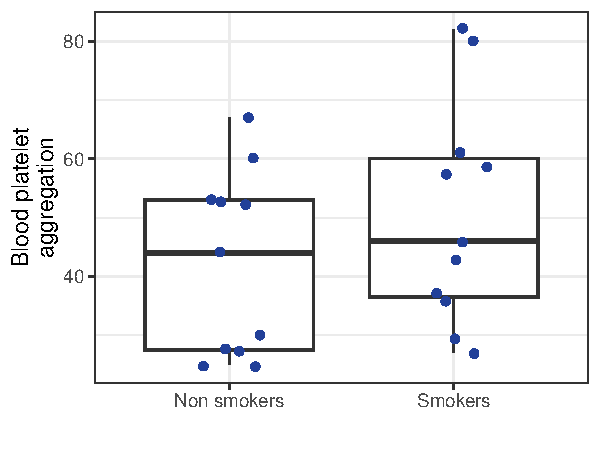
\includegraphics[width=\maxwidth]{figure/listings-unnamed-chunk-62-1} 

}

\end{Schunk}
\begin{redbox}{Workflow: Two sample \( t \)-test}
	\begin{itemize}
		\item \textbf{Hypotheses}: \( H_0: \mu_x = \mu_y \) vs \( H_1: \mu_x > \mu_y, \mu_x < \mu_y \) or \( \mu_x \neq \mu_y \)
		\item \textbf{Assumptions}: \( X_1,\dots,X_{n_x} \) are iid \( \mathcal{N} (\mu_X,\sigma^2) \), \( Y_1,\dotsc,Y_{n_y} \) are idd \( \mathcal{N} (\mu_Y,\sigma^2) \) and \( X_i \)'s are independent of \( Y_i \)'s.
		\item \textbf{Test Statistic}: \( T = \frac{\overline{X} - \overline{Y}}{S_p \sqrt{\frac{1}{n_x}+\frac{1}{n_y}}} \) where \( S^2_p = \frac{(n_x -1)S^2_x + (n_{y-1})S^2_y}{n_x + n_y -2} \). Under \( H_0, T \sim t_{n_x + n_y - 2} \) 
		\item \textbf{Observed Test Statistic}: \( t_0 = \frac{\overline{x} - \overline{y}}{s_p \sqrt{\frac{1}{n_x}+\frac{1}{n_y}}} \) where \( s^2_p = \frac{(n_x -1)s^2_x + (n_{y-1})s^2_y}{n_x + n_y -2} \).
		\item \textbf{p-value}: \( P(t_{n_x + n_y - 2} \geq t_0) \) or \( P(t_{n_x + n_y -2} \leq t_0) \) or \( 2P(t_{n_x + n_y - 2} \geq \lvert t_0 \rvert) \).
		\item \textbf{Decision}: If the p-value is less than \( \alpha \), there is evidence against \( H_0 \). If the p-value is greater than \( \alpha \), the data are consistent with \( H_0 \).
	\end{itemize}
\end{redbox}
Let \( X_i \) be the blood platelet aggregation levels for the \( i \)th non-smoker and \( Y_j \) the level for the \( j \)th smoker. Let \( \mu_S \) and \( \mu_N \) be the population mean platelet aggregation levels for smokers and non-smokers respectively.
\begin{itemize}
	\item \textbf{Hypotheses}: \( H_0: \mu_S = \mu_N \) vs \( H_1: \mu_S \neq \mu_N \)
	\item \textbf{Assumptions}: \( X_1,\dots,X_{n_x} \) are iid \( \mathcal{N} (\mu_X,\sigma^2) \), \( Y_1,\dotsc,Y_{n_y} \) are idd \( \mathcal{N} (\mu_Y,\sigma^2) \) and \( X_i \)'s are independent of \( Y_i \)'s.
	\item \textbf{Test Statistic}: \( T = \frac{\overline{X} - \overline{Y}}{S_p \sqrt{\frac{1}{n_x}+\frac{1}{n_y}}} \) Under \( H_0, T \sim t_{n_x + n_y - 2} \) 
	\item \textbf{Observed Test Statistic}: \( t_0 = \frac{50.6 - 42.2}{17.3 \sqrt{\frac{1}{11}+ \frac{1}{11}}} = 1.14 \).
	\item \textbf{p-value}: \( 2P(t_{20} \geq \lvert 1.14 \rvert) = 0.27 \).
	\item \textbf{Decision}: Large p-value so the data are consistent with \( H_0 \). There does not appear to be evidence that blood platelet aggregation levels are different in smokers.
\end{itemize}
\begin{Schunk}
\begin{Sinput}
t.test(smokers, non_smokers,
       alternative = "two.sided",
       var.equal = TRUE)
\end{Sinput}
\begin{Soutput}

	Two Sample t-test

data:  smokers and non_smokers
t = 1.144, df = 20, p-value = 0.2661
alternative hypothesis: true difference in means is not equal to 0
95 percent confidence interval:
 -6.961816 23.870907
sample estimates:
mean of x mean of y 
 50.63636  42.18182 
\end{Soutput}
\end{Schunk}
\subsubsection{The equal variance assumption}
\begin{itemize}
	\item We assume that the two underlying normal populations \textit{have the same variance}.
	\item In this example, does this seem reasonable?
	\begin{table}[H]\centering
		\begin{tabular}{@{}lccc@{}}
		\toprule
		Status      & Mean & SD   & \( n \)   \\ \midrule
		Non Smokers & 42.2 & 15.6 & 11 \\
		Smokers     & 50.6 & 18.9 & 11 \\ \bottomrule
		\end{tabular}
	\end{table}
	\item These are a little different: are they so different that the ``equal underlying population variances'' assumption is not reasonable?
\end{itemize}
\subsubsection{The Welch two-sample \( t \)-test}
\begin{itemize}
	\item Welch developed an alternative test which does \textbf{not} assume equal population variances. If
	\begin{itemize}
		\item the \( X_i \)'s are \( \mathcal{N} (\mu_X,\sigma^2_X) \) and
		\item the \( Y_i \)'s are \( \mathcal{N} (\mu_Y,\sigma^2_Y) \) then the variance of the sample mean difference is
		\[
			\var (\overline{X} - \overline{Y}) = \var(\overline{X}) + \var(\overline{Y}) = \frac{\sigma^2_X}{n_X} + \frac{\sigma^2_Y}{n_Y}
		\]
	\end{itemize}
	\item The standard error, \( \mathrm{SE} (\overline{X} - \overline{Y}) \), is obtained by plugging in the two sample variances and taking the square root (note: we do not need to compute a ``pooled'' estimate of the common variance!).
	\item This gives the \textit{Welch Statistic}, \( T = \frac{\overline{X} - \overline{Y}}{\sqrt{\frac{S^2_X}{n_x}+\frac{S^2_T}{n_y}}} \). 
\end{itemize}
\begin{redbox}{Workflow: Welch two sample \( t \)-test}
	\begin{itemize}
		\item \textbf{Hypotheses}: \( H_0: \mu_x = \mu_y \) vs \( H_1: \mu_x > \mu_y, \mu_x < \mu_y \) or \( \mu_x \neq \mu_y \)
		\item \textbf{Assumptions}: \( X_1,\dots,X_{n_x} \) are iid \( \mathcal{N} (\mu_X,\sigma^2) \), \( Y_1,\dotsc,Y_{n_y} \) are idd \( \mathcal{N} (\mu_Y,\sigma^2) \) and \( X_i \)'s are independent of \( Y_i \)'s.
		\item \textbf{Test Statistic}: \( T = \frac{\overline{X} - \overline{Y}}{\sqrt{\frac{S^2_X}{n_x}+\frac{S^2_T}{n_y}}} \) where \( S^2_x \) and \( S^2_y \) are the sample variance of the \( X \) and \( Y \) samples, respectively. Under \( H_0, T \sim t_\nu \) approximately, where the degrees of freedom parameter, \( \nu \), is estimated from the data.
		\item \textbf{Observed Test Statistic}: \( t_0 = \frac{\overline{x} - \overline{y}}{\sqrt{\frac{1}{n_x}+\frac{1}{n_y}}} \).
		\item \textbf{p-value}: \( P(t_\nu \geq t_0) \) or \( P(t_\nu \leq t_0) \) or \( 2P(t_\nu \geq \lvert t_0 \rvert) \).
		\item \textbf{Decision}: If the p-value is less than \( \alpha \), there is evidence against \( H_0 \). If the p-value is greater than \( \alpha \), the data are consistent with \( H_0 \).
	\end{itemize}
\end{redbox}
\subsubsection{Welch statistic not a proper \( t \)-statistic}
\begin{itemize}
	\item Technically, this statistic is not a ``usual'' \( t \)-statistic since the denominator is not a scaled \( \chi^2 \) independent of the numerator.
	\item However, the statistic still has an approximate \( t \)-distribution where the degrees of freedom is not necessarily a whole number, and is estimated from the data.
	\item R does this for us using \lstinline|var.equal = FALSE| (which is the default):
\end{itemize}
\begin{Schunk}
\begin{Sinput}
t.test(smokers, non_smokers, alternative = "two.sided")
\end{Sinput}
\begin{Soutput}

	Welch Two Sample t-test

data:  smokers and non_smokers
t = 1.144, df = 19.313, p-value = 0.2666
alternative hypothesis: true difference in means is not equal to 0
95 percent confidence interval:
 -6.997031 23.906122
sample estimates:
mean of x mean of y 
 50.63636  42.18182 
\end{Soutput}
\end{Schunk}
\subsection{Paired Samples \( t \)-test}
\subsubsection{Smoking and aggregation (paired)}
Blood samples from 11 individuals \textbf{\textcolor{myred}{before and after}} they smoked a cigarette are used to measure aggregation of blood platelets.
\begin{Schunk}
\begin{Sinput}
before = c(25, 25, 27, 44, 30, 67, 53, 53, 52, 60, 28)
after =  c(27, 29, 37, 36, 46, 82, 57, 80, 61, 59, 43)
df = data.frame(before, after, difference = after - before)
df
\end{Sinput}
\begin{Soutput}
   before after difference
1      25    27          2
2      25    29          4
3      27    37         10
4      44    36         -8
5      30    46         16
6      67    82         15
7      53    57          4
8      53    80         27
9      52    61          9
10     60    59         -1
11     28    43         15
\end{Soutput}
\end{Schunk}
Is the aggregation affected by smoking?
\begin{Schunk}
\begin{Sinput}
df |>
summarise(across(.cols = c(before, after), 
  .fns = list(Mean = mean, 
  SD = sd, 
  n = length))) |> 
pivot_longer(cols = everything(),
  names_sep = "_",
  names_to = c("time", ".value"))
\end{Sinput}
\begin{Soutput}
# A tibble: 2 x 4
  time    Mean    SD     n
  <chr>  <dbl> <dbl> <int>
1 before  42.2  15.6    11
2 after   50.6  18.9    11
\end{Soutput}
\begin{Sinput}
ggplot(df) +
aes(x = "", y = difference) + 
geom_boxplot() +
geom_dotplot(binaxis = "y", stackdir = "center") +
geom_hline(yintercept = 0, linetype = "dashed") +
labs(y = 'Difference in blood platelet levels')+
theme(axis.title.x = element_blank(),
  axis.text.x = element_blank(),
  axis.ticks.x = element_blank()) + 
theme_bw()
\end{Sinput}


{\centering 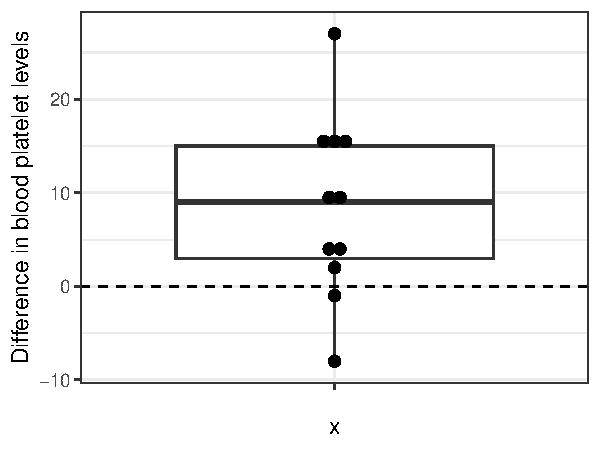
\includegraphics[width=\maxwidth]{figure/listings-unnamed-chunk-66-1} 

}

\end{Schunk}
\begin{Schunk}
\begin{Sinput}
t.test(df$after, df$before, paired = TRUE)
\end{Sinput}
\begin{Soutput}

	Paired t-test

data:  df$after and df$before
t = 2.9065, df = 10, p-value = 0.01566
alternative hypothesis: true mean difference is not equal to 0
95 percent confidence interval:
  1.97332 14.93577
sample estimates:
mean difference 
       8.454545 
\end{Soutput}
\begin{Sinput}
t.test(df$difference)
\end{Sinput}
\begin{Soutput}

	One Sample t-test

data:  df$difference
t = 2.9065, df = 10, p-value = 0.01566
alternative hypothesis: true mean is not equal to 0
95 percent confidence interval:
  1.97332 14.93577
sample estimates:
mean of x 
 8.454545 
\end{Soutput}
\end{Schunk}
Let \( X_i \) and \( Y_i \) be the blood platelet aggregation levels for the \( i^{\text{th}} \) person before and after smoking, respectively. Define the change in person \( i \)'s platelet aggregation as \( D_i = Y_i - X_i \) and the popultion mean change in platelet aggregation as \( \mu_d \) 
\begin{itemize}
	\item \textbf{Hypotheses}: \( H_0: \mu_d = 0 \) vs \( H_1: \mu_d \neq 0 \)
	\item \textbf{Assumptions}: \( D_i \) are iid \( \mathcal{N} (\mu_d,\sigma^2) \).
	\item \textbf{Test Statistic}: \( T = \frac{\overline{D}}{\sqrt{S_d / \sqrt{n}}} \). Under \( H_0, T \sim t_{n-1} \) 
	\item \textbf{Observed Test Statistic}: \( t_0 = \frac{8.45}{9.64 / \sqrt{11}} = 2.91 \).
	\item \textbf{p-value}: \( 2P(t_{10} \geq \lvert 2.91 \rvert) = 0.016 \).
	\item \textbf{Decision}: Small p-value so we have to reject the null hypothesis. There is evidence that blood platelet aggregation levels change after smoking.
\end{itemize}
\section{Critical values, rejection regions and confidence intervals}\label{sec:11}
\subsection{Random variables basics}
\begin{itemize}
	\item A random variable can be thought of as a mathematical object which takes certain values with certain probabilities.
	\item We have \textit{discrete} and \textit{continuous} random variables, although we can always ``approximate'' a continuous one with a discrete one (taking values on a suitably fine grid).
	\item A simple discrete random variable \( X \) can be described as a single random draw from a ``box'' containing tickets, each with numbers written on them.
	\item In this case,
	\begin{itemize}
		\item \( \mathrm{\mathrm{E}}(X) = \mu \) (the average of the numbers in the box),
		\item \( \var (X) = \sigma^2 \) (the \textit{population variance} of the numbers in the box), and
		\item \( \mathrm{SD} (X) = \sigma \).
	\end{itemize}
\end{itemize}
\subsubsection{Random sample with replacement}
\begin{itemize}
	\item Next, consider taking a random sample of size \( n \) \textit{with Replacement}, denote the values \( X_1,X_2,\dotsc,X_n \).
	\item This means, one of \textit{all possible samples of size} \( n \) is chosen in such a way that each is equally likely.
	\item If there are \( N \) tickets in the box, how many such samples are there?
	\item It turns out that these \( X_i \)'s are \textit{independent and identically distributed}. This means
	\begin{itemize}
		\item each \( X_i \) has the same distribution as a single draw,
		\item the \( X_i \)'s are all mutually independent.
	\end{itemize}
	\item Consider now taking the total \( T = \sum_{i=1}^{n} X_i \).
\end{itemize}
\subsubsection{Expectation of sums of random variables}
The \textbf{expectation} of a sum is \textit{always} the sum of the expectations.\\
Recall if \( \mathrm{E}(X) = \mu \),
\begin{align*}
	\mathrm{\mathrm{E}}(T) &= \mathrm{\mathrm{E}}(X_1 + \dotsb + X_n)\\
				  &= \mathrm{\mathrm{E}}(X_1) + \dotsb + \mathrm{\mathrm{E}}(X_n)\\
				  &= \underbrace{\mu + \dotsb + \mu}_{n\;\text{terms}}\\
				  &= n \mu
\end{align*}
\textbf{Multiplying by a constant}: for any random variable \( X \) and any constant \( c \),
\[
	\mathrm{\mathrm{E}}(cX) = c\mathrm{\mathrm{E}}(X)
\]
\subsubsection{Variance of sums of random variables}
The variance of a sum is \textit{not always} the sum of the variances.\\
However, it \textit{is} if the \( X_i \)'s are \textit{independent}. So,
\begin{align*}
	\var(T) &= \var(X_1 + \dotsb + X_n)\\
				  &= \var(X_1) + \dotsb + \var(X_n)\\
				  &= \underbrace{\sigma^2 + \dotsb + \sigma^{2}}_{n\;\text{terms}}\\
				  &= n \sigma^{2}.
\end{align*}
\textbf{Multiplying by a constant}: for any random variable \( X \) and any constant \( c \),
\[
	\var(cX) = c^{2}\var(X)
\]
\subsubsection{Sample mean}
Consider the sample mean \( \overline{X} = \frac{1}{n}\sum_{i=1}^{n} X_i = \frac{1}{n} T \).\\
What is \( \mathrm{\mathrm{E}}(\overline{X}) \)? What is \( Var(\overline{X}) \)?\\
Since \( \overline{X} = \frac{1}{n}T \),
\begin{align*}
	\mathrm{\mathrm{E}}(\overline{X}) &= \mathrm{\mathrm{E}}\left( \frac{1}{n} T \right) = \frac{1}{n} \mathrm{\mathrm{E}}(T) = \frac{1}{n} n \mu = \mu\\
	\var(\overline{X}) &= \var\left( \frac{1}{n} T \right) = \frac{1}{n}^{2} \var(T) = \frac{1}{n^{2}} n \sigma^{2} = \frac{\sigma^{2}}{n}
\end{align*}
\subsubsection{Estimating \( \mu \)}
\begin{itemize}
	\item In many applications, we model data \( x_1,\dotsc,x_n \) as values taken by such a sample \( X_1,\dotsc,X_n \) and we are interested in ``estimating'' or ``learning'' \( \mu \) (which is an ``unknown population mean'').
	\item In this case the \textit{estimator} is the sample mean \( \overline{X} \) (regarded as a \textit{random variable}).
	\item The \textit{estimate} is \( \overline{x} = \frac{1}{n} \sum_{i=1}^{n} x_i \), the observed value of the mean of the data (this is \textit{conceptually different} to \( \overline{X} \)!!)
	\item An important theoretical quantity is the \textit{standard error}, the \textit{standard deviation of the estimator}:
	\[
		\mathrm{SE} = \mathrm{SD}(\overline{X}) = \sqrt{\var(\overline{X})} = \frac{\sigma}{\sqrt{n}}
	\]
	\item The standard error is (in general) also an \textit{unknown parameter}.
\end{itemize}
\subsubsection{Importance of the standard error}
\begin{itemize}
	\item The standard error (standard deviation of the estimator) is important to know, since it tells us the ``likely size of the estimation error''.
	\item An estimate on its own is not very useful, we need to also know how accurate or reliable the estimate is.
	\begin{itemize}
		\item This is what the standard error provides.
	\end{itemize}
	\item \textit{Unfortunately} in most contexts the standard error is also \textit{unknown},
	\begin{itemize}
		\item but we can usually (also) estimate the standard error!
	\end{itemize}
\end{itemize}
\subsubsection{Estimating the standard error}
\begin{itemize}
	\item The standard error (at least when estimating a population mean \( \mu \)) involves the (usually unknown) population variance \( \sigma^2 \):
	\[
		\mathrm{SE} = \frac{\sigma}{\sqrt{n}}
	\]
	\item Fortunately, we can usually estimate \( \sigma^{2} \) using the \textit{sample variance}
	\[
		\mathrm{S}^{2} = \frac{1}{n-1} \sum_{i=1}^{n} (X_i - \overline{X})^2.
	\]
	\item The corresponding estimated standard error is
	\[
		\widehat{\mathrm{SE}} = \frac{s}{\sqrt{n}}
	\]
	where \( s^{2} = \frac{1}{n-1} \sum_{i=1}^{n} (x_i - \overline{x})^2. \)  is the observed value of the sample variance.
\end{itemize}
\subsection{Critical values and confidence intervals}
\subsubsection{More precise inference}
\begin{itemize}
	\item Usually, we want to know if a given value \( \mu_0 \) is a ``plausible value'' for the unknown \( \mu \), based on observed data \( x_1,\dotsc,x_n \).
	\item Roughly speaking, we do this by
	\begin{enumerate}
		\item computing the value of the estimate \( \overline{x} \),
		\item computing the value of the \textit{estimated standard error} \( \frac{s}{\sqrt{n}} \),
		\item seeing if the discrepancy \( \overline{x} - \mu_0 \) is ``large'' compared to the standard error.
	\end{enumerate}
	\item The various procedures we look at:
	\begin{itemize}
		\item \( t \)-tests (with corresponding p-values)
		\item confidence intervals
		\item rejection regions
	\end{itemize}
	are all variations on this single idea.
\end{itemize}
\subsubsection{What kind of discrepancies are of interest?}
\begin{itemize}
	\item We need to have it very clear in our minds which kind of discrepancies \( \overline{x} - \mu_0 \) we are interested in:
	\begin{itemize}
		\item positive
		\item negative
		\item both
	\end{itemize}
	\item Another way to think about it is, given a fixed \( \mu_0 \) of interest and an observed sample mean \( \overline{x} \), which of the following questions we are asking:
	\begin{enumerate}
		\item Is \( \overline{x} \) significantly \textit{more} then \( \mu_0 \)? (\textit{one-sided})
		\item Is \( \overline{x} \) significantly \textit{less} then \( \mu_0 \)? (\textit{one-sided})
		\item Is \( \overline{x} \) significantly \textit{different} then \( \mu_0 \)? (\textit{two-sided})
	\end{enumerate}
\end{itemize}
\subsubsection{Beer example}
Beer contents in a pack of six bottles (in millilitres) are:
\[
	374.8, 375.0, 375.3, 374.8, 374.4, 374.9
\]
\begin{goldbox}
	Does the mean beer content differ from the 375 ml claimed on the label?
\end{goldbox}
\begin{Schunk}
\begin{Sinput}
x = c(374.8, 375.0, 375.3, 374.8, 374.4, 374.9)
mean(x)
\end{Sinput}
\begin{Soutput}
[1] 374.8667
\end{Soutput}
\begin{Sinput}
sd(x)
\end{Sinput}
\begin{Soutput}
[1] 0.294392
\end{Soutput}
\end{Schunk}
\begin{itemize}
	\item In the beer example there are different possible points of view.
	\item For \textit{consumers}, the results will only be ``interesting'' if \( \overline{x} \) is significantly \textit{less} than 375:
	\begin{itemize}
		\item in this case the company is ``ripping consumers off''.
	\end{itemize}
	\item However for the \textit{beer} producers, both positive and negative discrepancies might be of interest:
	\begin{itemize}
		\item if they are \textit{underfilling}, consumers will be unhappy,
		\item if they are \textit{overfilling}, they are ``wasting'' some of their product.
	\end{itemize}
	\item Thus both a \textit{one-sided} and \textit{two-sided} point of view are conceivable even for this example.
\end{itemize}
\subsubsection{Two-sided discrepancies of interest}
When two-sided discrepancies are of interest we are basically asking: for a given \( \mu_0 \), is the \textit{absolute value} \( \lvert \overline{x} - \mu_0  \rvert \) large, compared to the standard error \( \frac{s}{\sqrt{n}} \)?
\begin{tcbraster}[raster columns = 2, raster halign = center, raster equal height=rows, enhanced, sharp corners, colback=white, coltitle=black, colbacktitle=myblue!25, sharpish corners, fonttitle=\bfseries, boxrule=0pt, borderline west={2pt}{0pt}{myblue}]
	\begin{tcolorbox}[title=\( t \)-test Approach]
		Declare hypothesised mean value \( \mu_0 \) \textbf{not plausible} if
		\[
			\lvert \overline{x} - \mu_0 \rvert > c \frac{s}{\sqrt{n}}
		\]
		for some suitably chosen \( c \).
	\end{tcolorbox}
	\begin{tcolorbox}[title=Confidence Interval Approach]
		Set of \textbf{plausible values} for the unknown \( \mu \) is
		\[
			\overline{x} \pm c \frac{s}{\sqrt{n}},
		\]
		for some suitably chosen \( c \).
	\end{tcolorbox}
	\begin{goldbox}
		\textbf{If the same \( c \) is chosen in both approaches, the set of plausible values \textit{is the same}, i.e. \( \mu_0 \) in the confidence interval \( \Leftrightarrow \lvert \overline{x} - \mu_0 \rvert \leq \frac{cs}{\sqrt{n}} \) }
	\end{goldbox}
\end{tcbraster}
\subsubsection{How to choose the constant \( c \)?}
\begin{itemize}
	\item The constant \( c \) can be chosen in a sensible way in each context.
	\item \textcolor{mygreen}{\textbf{Testing:}} control the \textcolor{mygreen}{\textbf{false alam rate}}.
	\item \textcolor{myred}{\textbf{Confidence Intervals}}: control the \textcolor{myred}{\textbf{coverage probability}}.
	\begin{itemize}
		\item the coverage probability is commonly also called the confidence level and expressed as a percentage.
	\end{itemize}
\end{itemize}
\subsubsection{False alarm rate}
\begin{itemize}
	\item A ``\textcolor{mygreen}{\textbf{false alarm}}'' is when we ``reject incorrectly''.
	\item Using our current language it is when we ``reject a given value \( \mu_0 \)'' when we shouldn't
	\item That is, we declare \( \mu_0 \) ``not plausible'' when in fact it is the true value!
	\item We pick choose small \( 0 \leq \alpha \leq 1 \) for the desired ``\textcolor{mygreen}{\textbf{false alarm rate}}'' e.g. 0.05, 0.1.
	\item Choose \( c \) such that (if possible)
	\[
		P \left( \lvert \overline{X} - \mu_0 \rvert > c \frac{S}{\sqrt{n}} \right) = \alpha
	\]
	\item If this isn't possible then just try to ensure that this probability does not exceed \( \alpha \)!
	\item The \textcolor{mygreen}{\textbf{false alarm rate}} is also called the \textcolor{mygreen}{\textbf{significance level}}. 
\end{itemize}
\subsubsection{Normal population: use the \( t \)-distribution}
Under the special statistical model where the data are modelled as \textcolor{mygreen}{iid normal random variables}, we know that \textit{if the true population mean is indeed} \( \symbf{mu}_0 \) then the ratio
\[
	\frac{\overline{X} - \mu_0}{S / \sqrt{n}} \sim t_{n-1},
\]
and therefore we choose \( c \) such that,
\[
	P \left( \lvert \overline{X} - \mu_0 \rvert > c \frac{S}{\sqrt{n}} \right) = P \left( \frac{\lvert \overline{X} - \mu_0 \rvert}{S / \sqrt{n}} > c \right) = P(\lvert t_{n-1} \rvert > c) = \alpha
\]
\subsubsection{Finding quantiles in R}
In R, we get quantiles using the \lstinline|qDISTRIBUTION()| range of functions, for example, \lstinline|qt(p, df = k), qnorm(p), qchisq(p, df = k)| for normal and \( \chi^2 \)  distributions respectively.
\begin{Schunk}
\begin{Sinput}
qt(0.05, df = 5)
\end{Sinput}
\begin{Soutput}
[1] -2.015048
\end{Soutput}
\begin{Sinput}
qnorm(0.05)
\end{Sinput}
\begin{Soutput}
[1] -1.644854
\end{Soutput}
\end{Schunk}
\subsubsection{Using \lstinline|qt()|}
Note that if \( P(\lvert t_{n-1} \rvert > c) = \alpha \) then
\[
	P(\lvert t_{n-1} \rvert \leq c) = P(-c \leq t_{n-1} \leq c) = 1 - \alpha
\]
and
\[
	P(t_{n-1} < -c) + P(t_{n-1} > c) = 2P(t_{n-1} \leq c) = 1 - \frac{\alpha}{2}.
\]
For example,
\begin{itemize}
	\item \( \alpha = 0.05 \), we need \( c \) such that \( P(t_{n-1} \leq c) = 1 - 0.025 = 0.975 \) so we use \lstinline|c = qt(0.975, df = n-1)|
	\item \( \alpha = 0.1 \), we need \( c \) such that \( P(t_{n-1} \leq c) = 1 - 0.005 = 0.995 \) so we use \lstinline|c = qt(0.995, df = n-1)|
\end{itemize}
\subsubsection{Beer example}
\begin{itemize}
	\item Recall we have observations
\begin{Schunk}
\begin{Sinput}
x = c(374.8, 375.0, 375.3, 374.8, 374.4, 374.9)
\end{Sinput}
\end{Schunk}
	\item Here the sample size \( n = 6 \) so if
	\begin{itemize}
		\item \( \alpha = 0.05 \) we neec \( c \) such that \( P(t_5 < c) = 0.975 \),
		\item \( \alpha = 0.1 \) we neec \( c \) such that \( P(t_5 < c) = 0.995 \) 
	\end{itemize}
	\item These are given by
\begin{Schunk}
\begin{Sinput}
qt(0.975, df = 5)
\end{Sinput}
\begin{Soutput}
[1] 2.570582
\end{Soutput}
\begin{Sinput}
qt(0.995, df = 5)
\end{Sinput}
\begin{Soutput}
[1] 4.032143
\end{Soutput}
\end{Schunk}
	\item The sample mean is
\begin{Schunk}
\begin{Sinput}
xbar = mean(x)
xbar
\end{Sinput}
\begin{Soutput}
[1] 374.8667
\end{Soutput}
\end{Schunk}
	\item The standard error is
\begin{Schunk}
\begin{Sinput}
se = sd(x)/sqrt(6)
se
\end{Sinput}
\begin{Soutput}
[1] 0.120185
\end{Soutput}
\end{Schunk}
	\item The discrepancy from the ``given value'' 375 is
\begin{Schunk}
\begin{Sinput}
discrep=abs(xbar-375)
discrep 
\end{Sinput}
\begin{Soutput}
[1] 0.1333333
\end{Soutput}
\end{Schunk}
	\item This is only slightly more than 1 (estimated) standard error.
	\item We need it to be at least 2.57 standard errors to ``reject at the 0.05 \textcolor{mygreen}{\textbf{false alarm rate}}'':
	\item Therefore we cannot reject \( H_0 \), so 375 is a plausible value (in this two-sided sense).
\end{itemize}
\subsubsection{Coverage probability}
\begin{itemize}
	\item For a \textcolor{myred}{\textbf{confidence interval}}, the \textcolor{myred}{\textbf{coverage probability}} is simply the probability that the ``true'' value of the unknown parameter lies inside (is ``covered by'') the \textcolor{mygreen}{\textbf{confidence interval}}.
	\item This is a \textit{long run property} and should be interpreted in the context of \textit{repeated experiments}.
	\item We choosea (small) \textit{non-coverage} probability \( \alpha \), say 0.05 or 0.01,
	\begin{itemize}
		\item then the \textcolor{myred}{\textbf{coverage probability}} is \( 1-\alpha \). 
	\end{itemize}
	\item Thus, under some statistical model we choose \( c \) so tht the  \textcolor{myred}{\textbf{coverage probability}} \textit{under the model} satisfies (with \( \mu \) the \textit{true population mean}):
\end{itemize}
\[
	P \left( \overline{X} - c \frac{S}{\sqrt{n}} \leq \mu \leq \overline{X} + c \frac{S}{\sqrt{n}} \right) = P \left( \lvert \overline{X} - \mu \rvert \leq c \frac{S}{\sqrt{n}} \right) = 1 - \alpha
\]
\subsubsection{Equivalent to false alarm rate condition for \( t \)-test}
\begin{itemize}
	\item The \textcolor{myred}{\textbf{coverage probability}} condition on the previous slide is an equivalent statement to the \textcolor{mygreen}{\textbf{false alarm rate}}  condition for the \( t \)-test (for the same \( \alpha \)).
	\item Thus if the desired \textcolor{myred}{\textbf{coverage probability}} is
	\begin{itemize}
		\item 0.95 (i.e. non-coverage probability \( \alpha = 0.05 \)) then we need \( c \) such that
		\[
			P(t_{n-1} \leq c) = 1 =0.025 = 0.975
		\]
		\item 0.99 (i.e. non-coverage probability \( \alpha = 0.1 \)) then we need \( c \) such that
		\[
			P(t_{n-1} \leq c) = 1 =0.005 = 0.995
		\]
	\end{itemize}
\end{itemize}
\subsubsection{Beer example}
\begin{minipage}[t]{0.49\textwidth}
For a 95\% confidence interval for \( \mu \) we thus choose \( c \) via
\begin{Schunk}
\begin{Sinput}
c_95 = qt(0.975, df = 5)
c_95
\end{Sinput}
\begin{Soutput}
[1] 2.570582
\end{Soutput}
\end{Schunk}
giving
\begin{Schunk}
\begin{Sinput}
xbar + c(-1,1) * c_95 * se
\end{Sinput}
\begin{Soutput}
[1] 374.5577 375.1756
\end{Soutput}
\end{Schunk}
Note that this includes the ``special value'' 375 and so is consistent with our 0.05 \textcolor{mygreen}{\textbf{false-alarm rate}} test earlier.
\end{minipage}
\hspace{0.02\textwidth}
\begin{minipage}[t]{0.49\textwidth}
For a 99\% confidence interval for \( \mu \) we thus choose \( c \) via
\begin{Schunk}
\begin{Sinput}
c_99 = qt(0.995, df = 5)
c_99
\end{Sinput}
\begin{Soutput}
[1] 4.032143
\end{Soutput}
\end{Schunk}
giving
\begin{Schunk}
\begin{Sinput}
xbar + c(-1,1) * c_99 * se
\end{Sinput}
\begin{Soutput}
[1] 374.3821 375.3513
\end{Soutput}
\end{Schunk}
As we'd expect, this CI is wider, and also includes 375.
\end{minipage}
\subsubsection{Using \lstinline|t.test|}
Compare our `manual' computations above with the output of the R function \lstinline|t.test()|:\\
\begin{minipage}[t]{0.49\textwidth}
First the default:
\begin{Schunk}
\begin{Sinput}
t.test(x, mu = 375)
\end{Sinput}
\begin{Soutput}

	One Sample t-test

data:  x
t = -1.1094, df = 5, p-value = 0.3177
alternative hypothesis: true mean is not equal to 375
95 percent confidence interval:
 374.5577 375.1756
sample estimates:
mean of x 
 374.8667 
\end{Soutput}
\end{Schunk}
\end{minipage}
\hspace{0.02\textwidth}
\begin{minipage}[t]{0.49\textwidth}
Setting \lstinline|conf.level-0.99|
\begin{Schunk}
\begin{Sinput}
t.test(x, mu = 375, conf.level = 0.99)
\end{Sinput}
\begin{Soutput}

	One Sample t-test

data:  x
t = -1.1094, df = 5, p-value = 0.3177
alternative hypothesis: true mean is not equal to 375
99 percent confidence interval:
 374.3821 375.3513
sample estimates:
mean of x 
 374.8667 
\end{Soutput}
\end{Schunk}
\end{minipage}
Note the default in R is \textit{two-sided}.
\subsubsection{One-sided discrepancies of interest}
\begin{itemize}
	\item The ``two-sided'' approach just outlined would be of interest to the beer producers, but not necessarily the beer consumers.
	\item Let us consider the point of view of the consumers now.
	\item \( t \)-test approach: declare (for some suitable value of \( c \)),
	\begin{itemize}
		\item \( \mu_0 \) \textcolor{mygreen}{not plausible} if \( \overline{x} - \mu_0 < -c \frac{s}{\sqrt{n}} \Leftrightarrow \overline{x} < \mu_0 - c \frac{s}{\sqrt{n}} \) 
	\end{itemize}
	\item \textcolor{myred}{\textbf{Confidence interval}} approach: set of plausible values for the unknown \( \mu \) are those ``not too much bigger than \( \overline{x} \)'' i.e.
	\[
		\bigg( -\infty, \overline{x} + c \frac{s}{\sqrt{n}} \bigg]
	\]
	for a ``suitably chosen'' constant \( c \) 
	\begin{itemize}
		\item the upper endpoint is sometimes called an ``upper confidence limit''
		\item it can be interpreted as ``the largest value consistent with the data''
	\end{itemize}
\end{itemize}
\subsubsection{Same set of plausible values}
\begin{itemize}
	\item Again, note that for the same \( c \) these two approaches give the \textit{same set of plausible values} for \( \mu \):
	\begin{itemize}
		\item \( \mu_0 \) is in the one-sided \textcolor{myred}{\textbf{confidence interval}} \( \Leftrightarrow \overline{x} \geq \mu_0 - c \frac{s}{\sqrt{n}} \).
	\end{itemize}
\end{itemize}
\subsubsection{Controlling the (one-sided) false alarm rate}
\begin{itemize}
	\item We use a similar approach to the two-sided case, but with a crucial difference!
	\item Under the iid normal model, \( T = \frac{\overline{X} - \mu}{S / \sqrt{n}} \sim t_{n-1} \)
	\item We choose \( c \) so that if \( \mu_0 \) is the true value,
	\[
		P \left( \overline{X} \leq \mu_0 - c \frac{S}{\sqrt{n}} \right) = P \left( \frac{\overline{X} - \mu_0}{S / \sqrt{n}} \right) = P(t_{n-1} < -c) = \alpha
	\]
	\item By symmetry we also have \( P(t_{n-1} > c) = \alpha \) or \( P(t_{n-1} < -c) = 1 -\alpha \) 
	\item For \textcolor{mygreen}{\textbf{false alarm rate}}
	\begin{itemize}
		\item 0.05 we need \( c \) such that \( P(t_{n-1} \leq c) = 1-0.05 = 0.95 \),
		\item 0.01 we need \( c \) such that \( P(t_{n-1} \leq c) = 1-0.01 = 0.99 \).
	\end{itemize}
\end{itemize}
\subsubsection{Beer example}
For the \( \alpha = 0.05 \) \textcolor{mygreen}{\textbf{false alarm rate}}, since \( n = 6 \) we need
\begin{Schunk}
\begin{Sinput}
c_05 = qt(.95, df = 5)
c_05
\end{Sinput}
\begin{Soutput}
[1] 2.015048
\end{Soutput}
\end{Schunk}
Note this is \textit{smaller} than the two-sided version.
We have already seen that the discrepancy is only slightly more than 1 standard error:
\begin{Schunk}
\begin{Sinput}
c(xbar - 375, se)
\end{Sinput}
\begin{Soutput}
[1] -0.1333333  0.1201850
\end{Soutput}
\end{Schunk}
For the \( \alpha = 0.01 \) \textcolor{mygreen}{\textbf{false alarm rate}}, since \( n = 6 \) we need
\begin{Schunk}
\begin{Sinput}
c_01 = qt(.99, df = 5)
c_01
\end{Sinput}
\begin{Soutput}
[1] 3.36493
\end{Soutput}
\end{Schunk}
Note that this is also smaller than the two-sided version.\\
This makes the one-sided tests ``more sensitive'' than the two-sided versions.
\subsubsection{One-sided confidence intervals}
Again we fix the \textcolor{myred}{\textbf{coverage probability}} \(  1-\alpha \):
\begin{align*}
	P \left( \mu_0 \leq \overline{x} + c \frac{S}{\sqrt{n}} \right) &= P \left( \frac{\overline{X} - \mu_0}{S / \sqrt{n}} \geq -c \right)\\
	&= P(t_{n-1} \geq -c)\\
	&= P(t_{n-1} \leq +c)\\
	&= 1-\alpha
\end{align*}
which is again the same as the corresponding \textcolor{mygreen}{\textbf{false alarm rate}} condition.\\
Thus for non-coverage probability
\begin{itemize}
	\item 0.05 we need \( c \) such that \( P(t_{n-1} \leq c) = 1-0.05 = 0.95 \),
	\item 0.01 we need \( c \) such that \( P(t_{n-1} \leq c) = 1-0.01 = 0.99 \).
\end{itemize}
\subsubsection{Beer example}
The 95\% ``upper confidence limit'' is
\begin{Schunk}
\begin{Sinput}
c_05 = qt(.95, df = 5)
xbar + c_05 * se
\end{Sinput}
\begin{Soutput}
[1] 375.1088
\end{Soutput}
\end{Schunk}
which gives the one-sided \textcolor{myred}{\textbf{confidence interval}}
\begin{Schunk}
\begin{Sinput}
c(-Inf, xbar + c_05 * se)
\end{Sinput}
\begin{Soutput}
[1]     -Inf 375.1088
\end{Soutput}
\end{Schunk}
For 99\%
\begin{Schunk}
\begin{Sinput}
c_01 = qt(.99, df = 5)
c(-Inf, xbar + c_01 * se)
\end{Sinput}
\begin{Soutput}
[1]     -Inf 375.2711
\end{Soutput}
\end{Schunk}
These both include 375!
\subsubsection{Using \lstinline|t.test()|}
\begin{Schunk}
\begin{Sinput}
t.test(x, mu = 375, alternative = "less")
\end{Sinput}
\begin{Soutput}

	One Sample t-test

data:  x
t = -1.1094, df = 5, p-value = 0.1589
alternative hypothesis: true mean is less than 375
95 percent confidence interval:
     -Inf 375.1088
sample estimates:
mean of x 
 374.8667 
\end{Soutput}
\begin{Sinput}
t.test(x, mu = 375, alternative = "less", conf.level = 0.99)
\end{Sinput}
\begin{Soutput}

	One Sample t-test

data:  x
t = -1.1094, df = 5, p-value = 0.1589
alternative hypothesis: true mean is less than 375
99 percent confidence interval:
     -Inf 375.2711
sample estimates:
mean of x 
 374.8667 
\end{Soutput}
\end{Schunk}
\subsubsection{Observed significance level: the p-value}
\begin{itemize}
	\item Finally, to tie all of this together we relate it all to the p-value.
	\item The observed significance level (or p-value) is the value of \( \alpha \) for which the observed data is ``right on the edge''.
	\item More precisely that is
	\begin{itemize}
		\item the smallest \textcolor{mygreen}{\textbf{false alarm rate}} for which we would ``reject'' a given value \( \mu_0 \),
		\item the \textit{non-coverage probability} (i.e. \( 1 - \) confidence level) for which \( \mu_0 \) is on the boundary of the \textcolor{myred}{\textbf{confidence interval}}
	\end{itemize}
\end{itemize}
\subsubsection{Beer example}
Using the (two sided) p-value in our level of confidence gives us a confidence interval ``right on the edge''.
\begin{Schunk}
\begin{Sinput}
t.test(x, mu = 375, conf.level = 1 - 0.3177)
\end{Sinput}
\begin{Soutput}

	One Sample t-test

data:  x
t = -1.1094, df = 5, p-value = 0.3177
alternative hypothesis: true mean is not equal to 375
68.23 percent confidence interval:
 374.7333 375.0000
sample estimates:
mean of x 
 374.8667 
\end{Soutput}
\end{Schunk}
Using the (one sided) p-value in our level of confidence gives us a confidence interval ``right on the edge''.
\begin{Schunk}
\begin{Sinput}
t.test(x, mu = 375, alternative = "less", conf.level = 1 - 0.1589)
\end{Sinput}
\begin{Soutput}

	One Sample t-test

data:  x
t = -1.1094, df = 5, p-value = 0.1589
alternative hypothesis: true mean is less than 375
84.11 percent confidence interval:
 -Inf  375
sample estimates:
mean of x 
 374.8667 
\end{Soutput}
\end{Schunk}
\subsection{Rejection regions}
\subsubsection{Decision rules}
	\begin{itemize}
		\item To test a hypothesis, we previously defined a \textbf{decision rule} to reject \( H_0 \). That is when the p-value is less than certain fixed preassigned levels, say p-value \( \leq \alpha \) where \( \alpha = 0.05, 0.10 \) etc
		\item In other words, we reject or do not reject or do not reject \( H_0 \) according to whether the p-value is less than or greater than \( \alpha \).
		\item The \( \alpha \) is called the significance level of the test, which is the boundary between rejecting and not rejecting \( H_0 \).
	\end{itemize}
\subsubsection{Notation}
Let \( t_{n-1} (\alpha) \) be the \textbf{critcal value} (or quantile given by)
\[
	P(t_{n-1} \le t_{n-1}(\alpha))=\alpha,
\]
or if we are using the standard normal distribution \(  Z \sim \mathcal{N} (0,1) \) then \( z(\alpha) \) is defined by \( P(Z \leq z(\alpha))=\alpha \).
\subsubsection{Critical value decision rule}
The critical value depends on the level of significance, \( \alpha \), and the distribution of \( T \) under \( H_0, t_{n-1} \)
\begin{greenbox}
	For a test of \( H_0: \mu = \mu_0 \) vs \( H_1: \mu > \mu_0 \), the \textbf{decision rule} at level \( \alpha \) is:
	\begin{itemize}
		\item reject \( H_0 \) if \( t_0 \geq t_{n-1} (1-\alpha) \) or equivalently reject \( H_0 \) if \( t_0 \geq \lvert t_{n-1} (\alpha) \rvert \) 
	\end{itemize}
	For a test of \( H_0: \mu = \mu_0 \) vs \( H_1: \mu < \mu_0 \), the \textbf{decision rule} at level \( \alpha \) is:
	\begin{itemize}
		\item reject \( H_0 \) if \( t_0 \leq \lvert t_{n-1} (\alpha) \rvert \) 
	\end{itemize}
	For a test of \( H_0: \mu = \mu_0 \) vs \( H_1: \mu \neq \mu_0 \), the \textbf{decision rule} at level \( \alpha \) is:
	\begin{itemize}
		\item reject \( H_0 \) if \( \lvert t_0 \rvert \geq \lvert t_{n-1} (\alpha / 2) \rvert \)
		\item do not reject \( H_0 \) if \( \lvert t_0 \rvert < \lvert t_{n-1} (\alpha / 2) \rvert \) 
	\end{itemize}
\end{greenbox}
\subsubsection{Rejection region for test statistics}
\begin{redbox}{Workflow: \( \sigma^2 \) unknown}
	\begin{itemize}
		\item \textbf{Hypothesis}: \( H_0: \mu = \mu_0 \) vs \( H_1: \mu > \mu_0, \mu < \mu_0, \mu \neq \mu_0 \)
		\item \textbf{Assumptions}: \( X_i \) are idd \( \mathcal{N}(\mu,\sigma^2) \), where \( \sigma^2 \) is \textcolor{myblue}{\textbf{unknown}}.
		\item \textbf{Test statistic}: \( T = \frac{\overline{X}-\mu_0}{S/\sqrt{n}} \sim t_{n-1} \)
		\item \textbf{Observed test statistic}: \( t_0 = \frac{\overline{x}-\mu_0}{s/\sqrt{n}} \)
		\item \textbf{Rejection region}:
		\item \begin{itemize}
			\item \( H_1: \mu \lessgtr \mu_0: t_0 \leq t_{n-1}(\alpha) \) or \( t_0 \geq \lvert t_{n-1}(\alpha) \rvert \)
			\item \( H_1: \mu \neq \mu_0: \lvert t_0 \rvert \geq \lvert t_{n-1} (\alpha / 2) \rvert \) 
		\end{itemize}
		\item \textbf{Decision}: We reject \( H_0 \) if \( t_0 \) is in the rejection region
	\end{itemize}
\end{redbox}
\begin{redbox}{Workflow: \( \sigma^2 \) known}
	\begin{itemize}
		\item \textbf{Hypothesis}: \( H_0: \mu = \mu_0 \) vs \( H_1: \mu > \mu_0, \mu \neq \mu_0 \)
		\item \textbf{Assumptions}: \( X_i \) are idd \( \mathcal{N}(\mu,\sigma^2) \), where \( \sigma^2 \) is \textcolor{myblue}{\textbf{known}}.
		\item \textbf{Test statistic}: \( T = \frac{\overline{X}-\mu_0}{\sigma/\sqrt{n}} \sim t_{n-1} \)
		\item \textbf{Observed test statistic}: \( z_0 = \frac{\overline{x}-\mu_0}{\sigma/\sqrt{n}} \)
		\item \textbf{Rejection region}:
		\begin{itemize}
			\item \( H_1: \mu \lessgtr \mu_0: z_0 \leq z(\alpha) \) or \( z_0 \geq \lvert z(\alpha) \rvert \)
			\item \( H_1: \mu \neq \mu_0: \lvert z_0 \rvert \geq \lvert z(\alpha / 2) \rvert \) 
		\end{itemize}
		\item \textbf{Decision}: We reject \( H_0 \) if \( z_0 \) is in the rejection region
	\end{itemize}
\end{redbox}
\subsubsection{Beer contents: testing using critical value}
We have \( n = 6, \overline{x} = 374.87, s = 0.29, t_0 = -1.11 \).
\begin{itemize}
	\item \textbf{Hypothesis}: \( H_0: \mu = 375 \) vs \( H_1: \mu < 375 \)
	\item \textbf{Assumptions}: \( X_i \) are idd rv \( \mathcal{N}(\mu,\sigma^2) \)
	\item \textbf{Test statistic}: \( T = \frac{\overline{X}-\mu_0}{\sigma/\sqrt{n}} \sim t_{n-1} \)
	\item \textbf{Observed test statistic}: \( t_0 = \frac{374.87 - 375}{0.29 /\sqrt{6}} = -1.11 \)
	\item \textbf{Critical value}: \( t_5 = (0.05) = \)  \lstinline|qt(0.05, df = 5)| \( = -2.015 \) i.e. reject if 
	is less than \( -2.015 \) 
	\item \textbf{Decision}: the observed test statistic, \( t_0 = -1.11 \), is greater than \( -2.015 \), so do not reject \( H_0 \)
\end{itemize}
\subsection{Rejection region on the data scale}
\subsubsection{Smoking and blood platelet aggregation}
Blood samples from 11 individuals before and after they smoked a cigarette are used to measure aggregation of blood platelets.

\begin{Schunk}
\begin{Sinput}
before = c(25, 25, 27, 44, 30, 67, 53, 53, 52, 60, 28)
after =  c(27, 29, 37, 36, 46, 82, 57, 80, 61, 59, 43)
df = data.frame(before, after, difference = after - before)
\end{Sinput}
\end{Schunk}
\begin{itemize}
	\item This is a match-pair sample.
	\item We reduce the data to one sample by considering the aggregation difference.
	\item Let \( X_i \) and \( Y_i \) be the blood platelet aggregation levels for the \( i^{\text{th}} \) person before and after smoking, respectively.
	\item Define the change in person \( i \)'s platelet aggregation levels as \( D_i = Y_i - X_i \) and the population mean change in platelet aggregation levels as \( \mu_d \) 
\end{itemize}
\begin{greenbox}
	\textbf{Is blood platelet aggregation affected by smoking?}
\end{greenbox}
\subsubsection{Rejection region for sample mean}
The rejection regions for the test using test statistic
\[
	t_0 = \frac{\overline{x} - \mu_0}{s/\sqrt{n}} \geq t_{n-1}(\alpha)
\]
on the standardised scale can be transformed to the measurement scale.
We can do this because\dots
\begin{align*}
	\alpha & = P\left( \frac{\overline{x} - \mu_0}{s/\sqrt{n}} \geq t_{n-1}(\alpha) \right) \\
	& = P\left( \overline{x} - \mu_0 \ge t_{n-1}(\alpha)s/\sqrt{n} \right) \\
	& = P\left( \overline{x} \ge t_{n-1}(\alpha)s/\sqrt{n} + \mu_0 \right)
\end{align*}
Which means we can define a rejection region on the measurement scale
\[
	\{\overline{x}: \overline{x} \ge k_0=\mu_0+t_{n-1}(\alpha) s/\sqrt{n} \} \quad \text{for} \quad  H_1\colon\ \mu > \mu_0.
\]
We have \( n = 11, \overline{d}=8.45, s_d = 9.65, t_0 = 2.91 \)
\begin{itemize}
	\item \textbf{Observed test statistic}: \( t_0 = \frac{\overline{d}}{s_d/\sqrt n} = \frac{8.45}{9.65/\sqrt{11}}= 2.91 \) 
	\item \textbf{Rejection region}: \( \left|\frac{\overline{d} - \mu_d}{ s_d/\sqrt{n} }\right| > t_{10}(0.025) = 2.228 \), rearranging,
	\begin{alignat*}{3}
		\overline{d} &< \mu_d - t_{n-1}(0.025) \, s_d/\sqrt{n} \qquad &&\overline{d}  &> \mu_d + t_{n-1}(0.025) \, s_d/\sqrt{n} \\
		\overline{d} &< 0 - 2.228 \times 9.65/\sqrt{11} \qquad &&\overline{d}  &> 0 + 2.228 \times 9.65/\sqrt{11} \\
		\overline{d} &< -6.48 \qquad &&\overline{d}  &> 6.48
		\end{alignat*}
	\item \textbf{Decision}: If \( \overline{d} < -6.48 \) or \( \overline{d} > 6.48 \) then reject \( H_0 \). In this case, \( \overline{d} = 8.45 > 6.48 \) so we reject \( H_0 \).
\end{itemize}
\begin{Schunk}
\begin{Sinput}
before = c(25, 25, 27, 44, 30, 67, 53, 53, 52, 60, 28)
after =  c(27, 29, 37, 36, 46, 82, 57, 80, 61, 59, 43)
df = data.frame(before, after, difference = after-before)
s_d = sd(df$difference)
s_d
\end{Sinput}
\begin{Soutput}
[1] 9.647421
\end{Soutput}
\begin{Sinput}
n = nrow(df)
mu0 = 0
crit_val = qt(0.975, df = n-1)
crit_val
\end{Sinput}
\begin{Soutput}
[1] 2.228139
\end{Soutput}
\begin{Sinput}
rrlower = mu0 - crit_val * s_d / sqrt(n)
rrupper = mu0 + crit_val * s_d / sqrt(n)
c(rrlower, rrupper) |> round(2)
\end{Sinput}
\begin{Soutput}
[1] -6.48  6.48
\end{Soutput}
\end{Schunk}
\subsubsection{Beer contents}
We have \( n = 6, \overline{d}=374.87, s_d = 0.29, t_0 = -1.11 \). Hypothesis test using rejection region with \( \alpha = 0.05 \).
\begin{itemize}
	\item \textbf{Hypothesis}: \( H_0: \mu = 375 \) vs \( H_1: \mu < 375 \)
	\item \textbf{Assumptions}: \( X_i \) are idd rv \( \mathcal{N}(\mu,\sigma^2) \)
	\item \textbf{Test statistic}: \( T = \frac{\overline{X}-\mu_0}{\sigma/\sqrt{n}} \sim t_{n-1} \)
	\item \textbf{Rejection region (on the data scale)}:
		\begin{align*}
		\frac{\overline{X} - \mu}{ s/\sqrt{n} } & < t_{n-1}(0.05)  \\
		\overline{X} & < \mu + t_{n-1}(0.05) \, s/\sqrt{n} \\
		\overline{X} & < 375 - 2.015 \times 0.29/\sqrt{6} \\
		\overline{X} & < 374.74
		\end{align*}
	\item \textbf{Decision}: the observed test statistic, \( \overline{x} = 374.9 \), is greater than \( 374.9 \), so do not reject \( H_0 \).
\end{itemize}
\section{Sample Size Calculations and Power}\label{sec:12}
\subsection{Power and sample size}
\subsubsection{Errors in hypothesis testing}
\begin{table}[H]
	\centering
	\begin{tabular}{@{}lll@{}}
	\toprule
	\textbf{}                       & \textbf{\( H_0 \) true (innocent)} & \textbf{\( H_0 \) false (guilty)} \\ \midrule
	Don't reject \( H_0 \) (acquit) & Correct decision                   & Type II error \( (\beta) \)       \\
	Reject \( H_0 \) (guilty)       & Type I error  \( (\alpha) \)       & Correct decision \( (1-\beta) \)  \\ \bottomrule
	\end{tabular}
\end{table}
\begin{itemize}
	\item Type I errors: level of significance, \( \alpha = P(\text{reject}\;H_0 \mid H_0\;\text{true}) \) 
	\item Type II errors: call it \( \beta \) 
	\item Power: \( 1 - \beta = P(\text{reject}\;H_0 \mid H_1\;\text{true}) \) 
\end{itemize}
\subsubsection{General testing setup}
\begin{itemize}
	\item Interested in inference concerning an unknown population mean \( \mu \)
	\item We are considering a fixed value \textcolor{myblue}{\( \mu_0 \)} (``\textcolor{myblue}{\textbf{hypothesised value}}'')
	\item We then observe the data \( x_1, \dotsc, x_n \), obtaining
	\begin{itemize}
		\item the sample mean \( \overline{x} \)
		\item the sample sd \( s \) and thus the \textit{estimated standard error} (se) \( s / \sqrt{n} \) 
	\end{itemize}
	\item We decide to perform a (say, two-sided) \( t \)-test, that is to say if the \textit{observed discrepancy} \( \overline{x} - \textcolor{myblue}{\mu_0} \)  is \textit{large} compared to the se, we will ``reject'' the value \textcolor{myblue}{\( \mu_0 \)} as ``implausible''
	\[
		\text{Reject if}\; \lvert \overline{x} - \textcolor{myblue}{\mu_0 \rvert > c  \frac{s}{\sqrt{n}}},
	\]
	where \( c \) is chosen so that the false alarm rate is some fixed, small value \( \alpha \) (e.g. 0.05, 0.01).
\end{itemize}
\subsubsection{Model assumptions}
\begin{itemize}
	\item The \textcolor{myred}{\textbf{false alarm rate}} determination can only be made if a suitable statistical model is assumed for the data.
	\item If we model the data \( x_1, \dotsc, x_n \) as values taken by iid \( \mathcal{N}(\mu,\sigma^2) \) random variables \( X_1, \dotsc, X_n \) (with \( \mu \) and \( \sigma^2 \) \textit{both unknown}), then whatever the true value \( \mu \) is we know, \( \frac{\overline{X}-\mu}{S/\sqrt{n}}\sim t_{n-1} \).
	\item The \textcolor{myred}{\textbf{false alarm rate}} is
	\[
		P_{\textcolor{myblue}{\mu_0}} \left( \left| \overline{X}-\textcolor{myblue}{\mu_0} \right| >c\frac{S}{\sqrt{n}} \right) = P_{\textcolor{myblue}{\mu_0}} \left( \frac{\left| \bar X-\textcolor{myblue}{\mu_0} \right|}{S/\sqrt{n}}>c \right)= P(|t_{n-1}|>c) = 2 P(t_{n-1}>c)
	\]where the final equality follows by symmetry of the 
	\( t_n-1 \) distribution.
	\item The \( P_{\textcolor{myblue}{\mu_0}}(\cdot) \) indicates probability when the true value is \( \textcolor{myblue}{\mu_0} \), i.e. the value we specified in the null hypothesis.
\end{itemize}
\subsubsection{Beer example}
\begin{itemize}
	\item Suppose we have \( n = 6 \) and choose a \textbf{false alarm rate} of \( \alpha = 0.05 \).
	\item Then the constant \( c \) needs to satisfy
	\[
		2P(t_5>c)=\alpha
	\]
	so
	\[
		P(t_5>c)=\alpha/2=0.025
	\]
	and thus
	\[
		P(t_5\leq c)=0.975.
	\]
\begin{Schunk}
\begin{Sinput}
c_05 = qt(0.975, df = 5)
c_05
\end{Sinput}
\begin{Soutput}
[1] 2.570582
\end{Soutput}
\end{Schunk}
\end{itemize}
\subsubsection{Why allow false alarms at all?}
\begin{itemize}
	\item A fair question is: \textit{why would you set things up to have 5\% \textbf{false alarm rate}}?
	\item Why not make it \textit{really small}, like \( 10^{-6} \)?
	\item \textit{Answer}: because then you would never reject anything, even if you should!
	\item The technical reason: because then the test would have no \textbf{power}.
\end{itemize}
\begin{bluebox}{Definition}
	The \textbf{power} of a test is the probability that the test rejects the null hypothesis, \( H_0 \) when a \textbf{specific} alternative hypothesis \( H_1 \) is true.
	\[
		\text{Power} = P(\text{reject}\; H_0 \mid H_1 \text{is true}).
	\]
\end{bluebox}
\subsubsection{Statistical power in one sample \( t \)-test}
\begin{itemize}
	\item Consider the probability of ``rejecting'' as a function of the true population mean \( \textcolor{myred}{\mu} \):
	\[
			P_{\textcolor{myred}{\mu}} \left(\text{reject }H_0\right) = P_{\textcolor{myred}{\mu}} \left( \left| \overline{X} -\textcolor{myblue}{\mu_0} \right| >c\frac{S}{\sqrt{n}} \right)=
			P_{\textcolor{myred}{\mu}} \left( \frac{\left| \overline{X} -\textcolor{myblue}{\mu_0}\right|}{S/\sqrt{n}}>c \right).
	\]
	\item This is the \textbf{statistical power function} of the test.
	\item To determine this we need to know the \textit{distribution} of the \( t \)-statistic for testing \( \textcolor{myblue}{\mu_0} \):
	\[
		\frac{\overline{X}- {\textcolor{myblue}{\mu_0}}}{S/\sqrt{n}}
	\]
	when the true population mean \( \textcolor{myred}{\mu} \) is not necessarily equal to \( \textcolor{myblue}{\mu_0} \) (the hypothesised population mean)!
\end{itemize}
\subsubsection{Beer example: power calculations}
\begin{itemize}
	\item Suppose the sample sd is \textit{indicative} of the ``true'' population standard deviation.
	\item We want to plot the power function of the test as a function of \( \textcolor{myred}{\mu} \).
	\item First let us assume the ``true'' \( \sigma \) is equal to the sample value.
\end{itemize}
\begin{Schunk}
\begin{Sinput}
x = c(374.8, 375.0, 375.3, 374.8, 374.4, 374.9)
sig = sd(x)  
sig
\end{Sinput}
\begin{Soutput}
[1] 0.294392
\end{Soutput}
\end{Schunk}
\subsubsection{Power as a function of true mean \( \textcolor{myred}{\mu} \)}
Given that we pick \( H_0: \mu = \textcolor{myblue}{375} \) 
\begin{Schunk}
\begin{Sinput}
mu = seq(374, 376, by = 0.01)
nu = (mu-375)/(sig/sqrt(6))
power_mu = pt(c_05, df = 5, ncp = nu, lower.tail = FALSE) + pt(-c_05, df = 5, ncp = nu)
power_df = data.frame(mu, nu, power = power_mu)
g1 = ggplot(data = power_df, aes(x=mu, y=power)) +
  geom_line() +
  labs (x = expression(mu),
        y = "Power") +
  geom_hline(yintercept = 0.05, colour = "#224099", linetype = "dashed") + 
  theme_bw()
g1
\end{Sinput}


{\centering 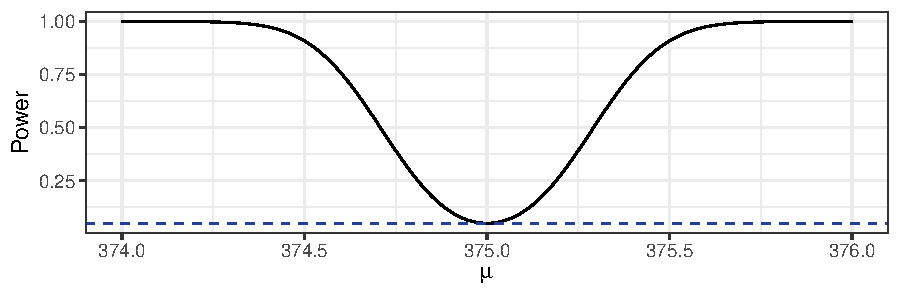
\includegraphics[width=\maxwidth]{figure/listings-unnamed-chunk-94-1} 

}

\end{Schunk}
The further the true mean \( \textcolor{myred}{\mu} \) is from the value \( \textcolor{myblue}{\mu_0} \) picked for the null hypothesis the more likely we are to reject.
\subsubsection{Discrepancy needed to achieve a certain power}
Assume:
\begin{itemize}
	\item population sd \( \sigma = 0.294 \) 
	\item sample size of \( n = 6 \)
	\item \( H_0: \mu = 375 \) vs \( \mu \neq 375 \) 
\end{itemize}
\begin{greenbox}
	\textbf{How much lower than 375 does \( \textcolor{myred}{\mu} \) need to be for us to be 80\% sure of ``detecting'' that \( \textcolor{myred}{\mu \neq 375} \) with a two-sided test which has false alarm rate 0.05?}
\end{greenbox}
\begin{Schunk}
\begin{Sinput}
g1 +
geom_hline(yintercept = 0.8, colour = "#224099",linewidth = 1) + 
geom_vline(xintercept = 374.6, colour = "#992240",linewidth = 1)
\end{Sinput}


{\centering 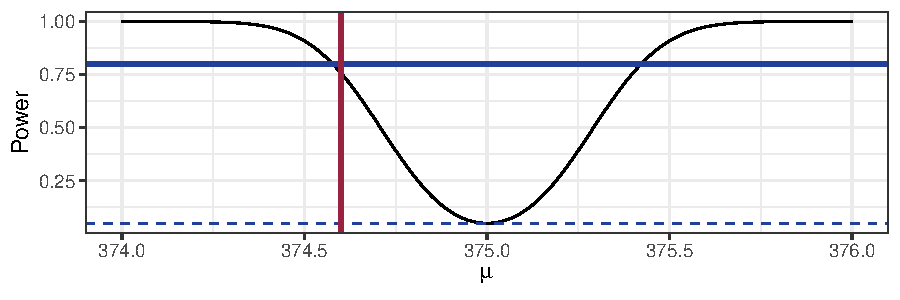
\includegraphics[width=\maxwidth]{figure/listings-unnamed-chunk-95-1} 

}

\end{Schunk}
\begin{itemize}
	\item The \( \textcolor{myred}{\mu} \) value with power 80\% is around 374.6.
\end{itemize}
\subsubsection{Comparing to false alarm rate of \( 10^{-6} \)}
For a two sided test with \( n = 6 \) and a \textbf{false alarm rate} of \( \alpha = 10^{-6} \), we need a critical value of
\begin{Schunk}
\begin{Sinput}
crit_val = qt(1 - (1e-6) / 2, df = 5)
crit_val
\end{Sinput}
\begin{Soutput}
[1] 28.47847
\end{Soutput}
\end{Schunk}
So we would need a discrepancy equal to more than 28 standard errors before we would reject 375!
\subsubsection{Power as a function of \( \alpha \)}
\begin{Schunk}
\begin{Sinput}
mu = seq(368, 382, by = 0.05)
nu = (mu-375)/(sig/sqrt(6))
power1 = pt(c_05, df = 5, ncp = nu, lower.tail = FALSE) + pt(-c_05, df = 5, ncp = nu)
power2 = pt(crit_val, df = 5, ncp = nu, lower.tail = FALSE) + pt(-crit_val, df = 5, ncp = nu)
power_df = data.frame(mu, nu, power1, power2)
ggplot(data = power_df, aes(x=mu)) +
  geom_line(aes(y = power1), colour = "#997b22") +
  geom_line(aes(y = power2), colour = "#7b2299") +
  labs (x = expression(mu),
        y = "Power") +
  geom_hline(yintercept = 0.8, colour = "#224099") +
  theme_bw()
\end{Sinput}


{\centering 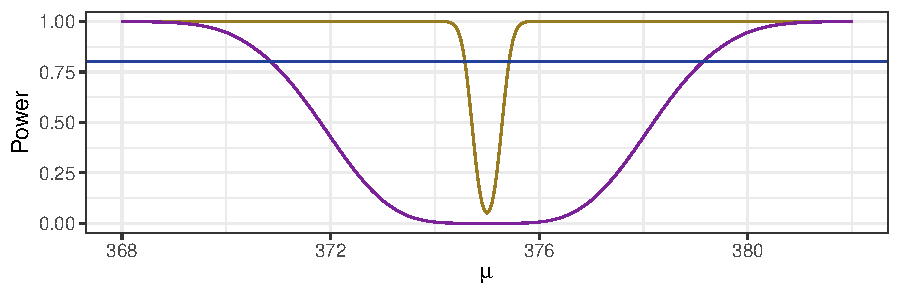
\includegraphics[width=\maxwidth]{figure/listings-unnamed-chunk-97-1} 

}

\end{Schunk}
To achieve a power of about 80\% with such a small false alarm rate, we would require a true \( \textcolor{myred}{\mu} \) lower than 371 or more than 379!
\subsubsection{Power as a function of \( n \)}
\begin{itemize}
	\item Now let us suppose that \textit{both} the sample mean and sample sd are indicative of the ``true'' values \( \textcolor{myred}{\mu} \) and \( \sigma \) 
\begin{Schunk}
\begin{Sinput}
xbar = mean(x)
c(xbar, sig)
\end{Sinput}
\begin{Soutput}
[1] 374.866667   0.294392
\end{Soutput}
\end{Schunk}
	\item Can we see how the power ought to behave as a function of \( n \)?
	\item \textit{Note} the degrees of freedom, and thus the critical value, change with \( n \).
\end{itemize}
\begin{Schunk}
\begin{Sinput}
power_n = data.frame(
  n = 6:100
) |> mutate(
  nu = (xbar-375)/(sig/sqrt(n)),
  c_05_n = qt(0.975, df = n-1),
  power = pt(c_05_n, df = n-1, ncp = nu, lower.tail = FALSE) + 
    pt(-c_05_n, df = n-1, ncp = nu) 
)
ggplot(data = power_n, aes(x = n, y = power)) +
  geom_line() +
  labs (x = "n",
        y = "Power(n)") +
  geom_hline(yintercept = 0.05, colour = "#224099", linetype = "dashed") + 
  theme_bw()
\end{Sinput}


{\centering 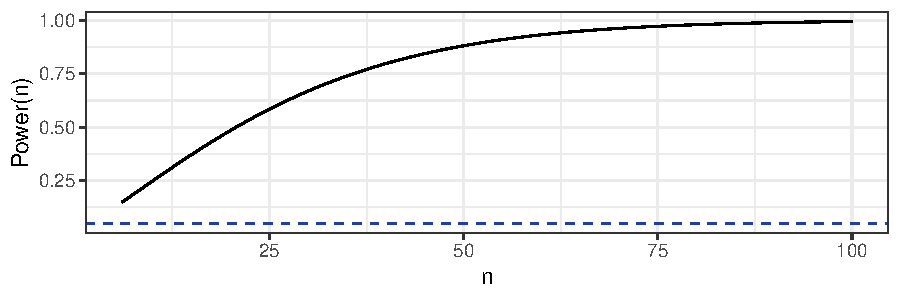
\includegraphics[width=\maxwidth]{figure/listings-unnamed-chunk-99-1} 

}

\end{Schunk}
Again, this is assuming the ``true'' values \( \textcolor{myred}{\mu} \) and \( \sigma \) equal the sample values \( \overline{x} \) and \( s \). But it is still useful!
\subsection{How to do it in R}
\subsubsection{There's a package for that}
The \textcolor{myred}{\textbf{pwr}} package (Champely, 2020).
\begin{Schunk}
\begin{Sinput}
library(pwr) 
\end{Sinput}
\end{Schunk}
The key functions:
\begin{itemize}
	\item \lstinline|pwr.t.test()| t-tests (one sample, 2 sample, paired)
	\item \lstinline|pwr.t2n.test()| t-test (two samples with unequal n)
\end{itemize}
\subsubsection{Cohen's d}
Rather than specifying a null mean and an alternative mean and standard deviation, the \textbf{pwr} functions take as an input ``Cohen's d'':
\[
	d = \frac{\lvert \mu_1 - \mu_2 \rvert}{\sigma}
\]
Cohen suggests that \( d \) values of 0.2, 0.5, and 0.8 represent small, medium, and large effect sizes respectively.
\subsubsection{Beer example}
\begin{itemize}
	\item Suppose the population sd \( \sigma = 0.294 \), with a sample size of \( n = 6 \) how much lower than 375 does \textcolor{myred}{\( \mu \)} need to be for us to be 80\% sure of ``detecting'' that \textcolor{myred}{\( \mu \neq 375 \)} with a \textit{two-sided} test which has \textbf{false alarm rate} 0.05?
\begin{Schunk}
\begin{Sinput}
res = pwr.t.test(n = 6, 
                 d = NULL, 
                 sig.level = 0.05, 
                 power = 0.8, 
                 type = "one.sample", 
                 alternative = "two.sided")
                 res$d * 0.294 # d * sigma gives the difference between means
\end{Sinput}
\begin{Soutput}
[1] 0.4217541
\end{Soutput}
\end{Schunk}
\[
	d = \frac{\lvert \mu_1 - \mu_2 \rvert}{\sigma} = 1.43 \implies \lvert \mu_1 - \mu_2 \rvert = 1.43\sigma = 0.42
\]
	\item Suppose the population  \textcolor{myred}{\( \mu = 374.87 \)} and \( \sigma = 0.294 \), what sample size \( n \) would be needed to be at least 80\% sure of detecting that \( \mu \neq 375 \) with a \textit{two-sided} test which has \textbf{false alarm rate} 0.05?
\begin{Schunk}
\begin{Sinput}
res = pwr.t.test(n = NULL,
                 d = (374.87-375)/0.294, 
                 sig.level = 0.05,
                 power = 0.8, 
                 type = "one.sample", 
                 alternative = "two.sided")
res
\end{Sinput}
\begin{Soutput}

     One-sample t test power calculation 

              n = 42.10456
              d = 0.4421769
      sig.level = 0.05
          power = 0.8
    alternative = two.sided
\end{Soutput}
\end{Schunk}
We would need at least 43 observations (round up from 42.1 because if we round down then the power will be less than 80\%).
\end{itemize}
\section{Sign test}\label{sec:13}
\subsection{Checking for normality}
\subsubsection{Normality}
\begin{itemize}
	\item The assumption that your data are \textcolor{mygreen}{sampled from a normal population} arises quite often.
	\item If you have a \textbf{large enough} sample size, then the normality assumption is not as important as you can usually rely on the central limit theorem to ensure your \textcolor{myred}{test statistic} at least approximately follows a \( t \)-distribution
	\item In \textcolor{mygreen}{small samples} it can be difficult to tell whether or not your sample comes from a normal population!
\end{itemize}
You can check the normality assumption using:
\begin{itemize}
	\item \textbf{QQ plots} (this is the best way to visually assess normality)
	\item \textbf{Boxplots} (most useful when only looking for symmetry)
	\item Formal hypothesis tests?
\end{itemize}
\subsubsection{Checking for normality: boxplots}
\begin{Schunk}
\begin{Sinput}
set.seed(88)
n_groups = 20
n_obs = 100
dat_100 = data.frame(
  values = rnorm(n_groups * n_obs),
  group = rep(letters[1:n_groups], each = n_obs)
)
ggplot(dat_100) + aes(x = group, y = values) + 
  geom_boxplot(fill = "#224099") + 
  labs(x = NULL, caption = "n=100 in each group") +
  theme_classic()
\end{Sinput}


{\centering 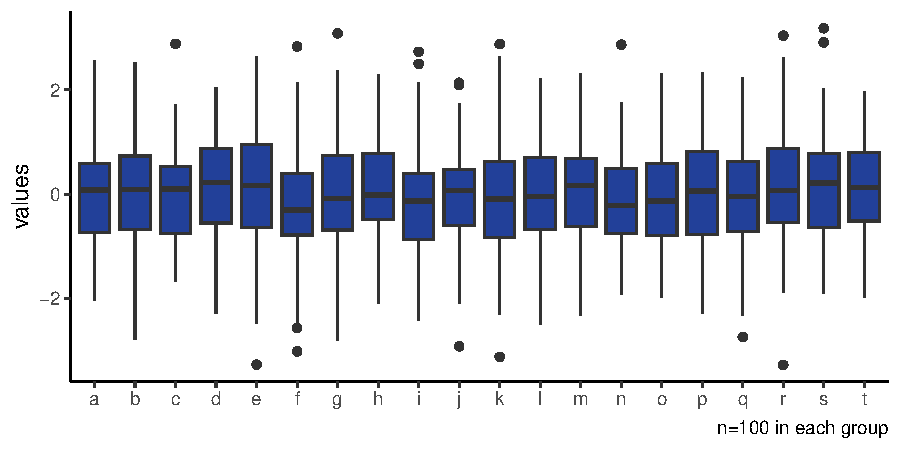
\includegraphics[width=\maxwidth]{figure/listings-unnamed-chunk-103-1} 

}

\end{Schunk}
\begin{Schunk}
\begin{Sinput}
set.seed(88)
n_groups = 20
n_obs = 10
dat_10 = data.frame(
  values = rnorm(n_groups * n_obs),
  group = rep(letters[1:n_groups], each = n_obs)
)
ggplot(dat_10) + aes(x = group, y = values) + 
  geom_boxplot(fill = "#224099") + 
  labs(x = NULL, caption = "n=10 in each group") +
  theme_classic()
\end{Sinput}


{\centering 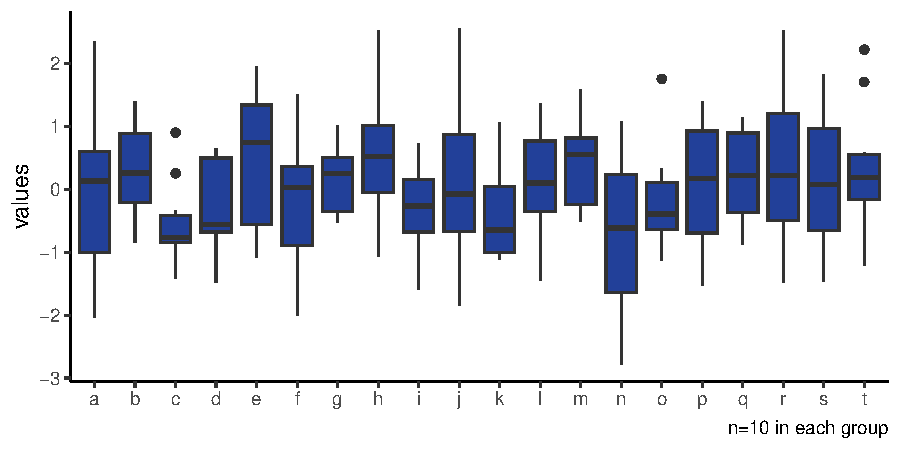
\includegraphics[width=\maxwidth]{figure/listings-unnamed-chunk-104-1} 

}

\end{Schunk}
\begin{tcolorbox}[bluestyleline]
	To check for normality in a boxplot, we're mostly looking for \textbf{symmetry}. But this is \textbf{hard}, particularly in small samples.
\end{tcolorbox}
\subsubsection{Checking for normality: QQ plots}
\begin{Schunk}
\begin{Sinput}
dat_100 |> dplyr::filter(group <= "h") |> 
  ggplot() + 
  aes(sample = values, group = group) + 
  geom_qq_line() + geom_qq() + 
  facet_wrap(~group, nrow = 2) +
  theme_classic()
\end{Sinput}


{\centering 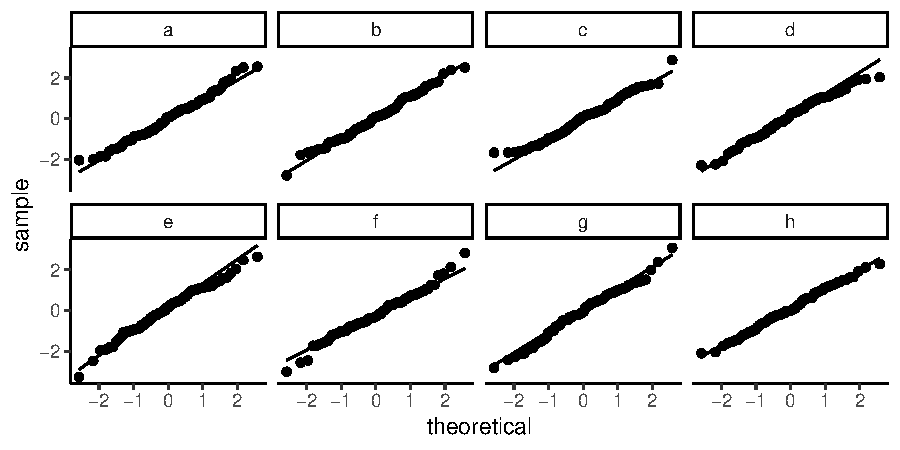
\includegraphics[width=\maxwidth]{figure/listings-unnamed-chunk-105-1} 

}

\end{Schunk}
These are QQ-plots, each with \textcolor{mygreen}{100} observations drawn from a normal population.
\begin{Schunk}
\begin{Sinput}
dat_10 |> dplyr::filter(group <= "h") |> 
  ggplot() + 
  aes(sample = values, group = group) + 
  geom_qq_line() + geom_qq() + 
  facet_wrap(~group, nrow = 2) +
  theme_classic()
\end{Sinput}


{\centering 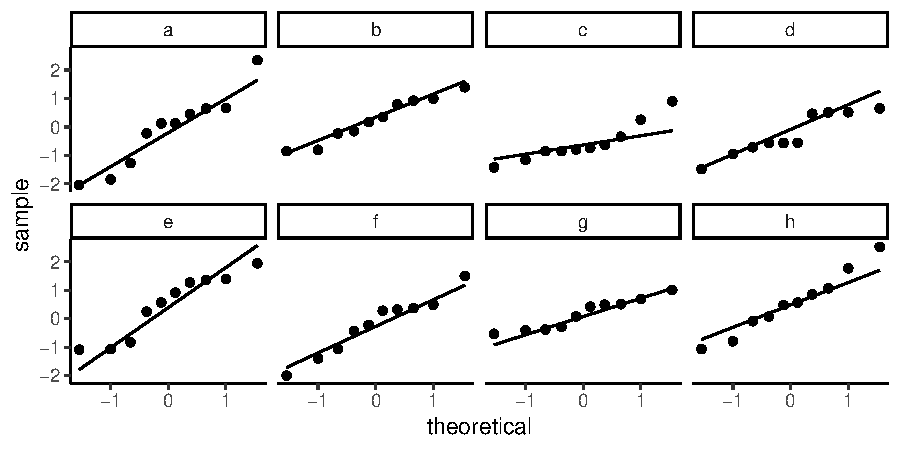
\includegraphics[width=\maxwidth]{figure/listings-unnamed-chunk-106-1} 

}

\end{Schunk}
These are QQ-plots, each with \textcolor{mygreen}{10} observations drawn from a normal population.\\
If we're checking for normality in a QQ plot, then we're mostly looking for \textbf{points that lie reasonably close to the line}.
\subsubsection{Rat data: normality}
\begin{Schunk}
\begin{Sinput}
rat = data.frame(
  bio = c(1.7, 2.0, 1.7, 1.5, 1.6, 
          2.4, 2.3, 2.4, 2.4, 2.6),
  pla = c(2.1, 1.8, 2.2, 2.2, 1.5, 
          2.9, 2.9, 2.4, 2.6, 2.5)
) |> mutate(d = pla - bio)
ggplot(rat) + aes(y = "", x = d) + 
  geom_boxplot() + 
  geom_jitter(width = 0.1, 
              size = 2,
              colour = "#224099") + 
  labs(y = "", 
       x = "Difference in muscle weight (g)") +
  theme_classic()
\end{Sinput}


{\centering 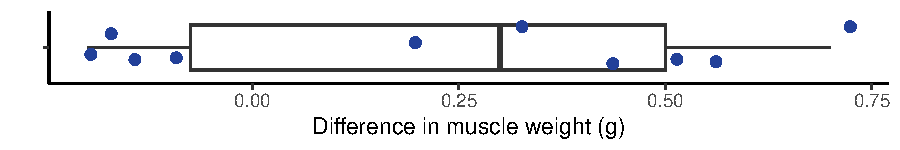
\includegraphics[width=\maxwidth]{figure/listings-unnamed-chunk-107-1} 

}

\end{Schunk}
\begin{Schunk}
\begin{Sinput}
ggplot(rat, aes(sample = d)) + 
  geom_qq(size = 3) +
  geom_qq_line() + 
  labs(x = "Theoretical quantiles",
       y = "Sample data") +
  theme_classic()
\end{Sinput}


{\centering 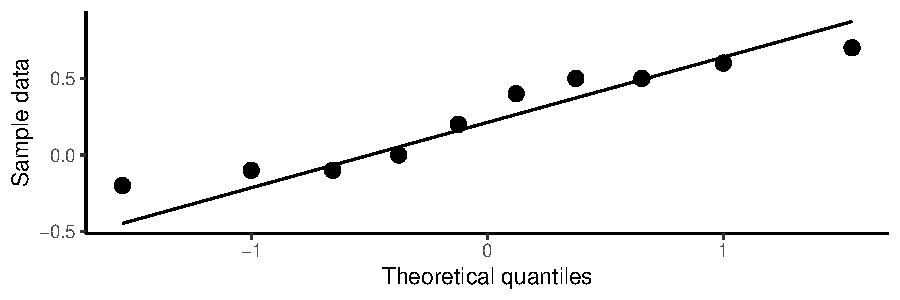
\includegraphics[width=\maxwidth]{figure/listings-unnamed-chunk-108-1} 

}

\end{Schunk}
\subsection{Sign test}
\begin{itemize}
	\item Suppose a sample \( X_1,\dotsc,X_n \) are independently sampled from a continuous distribution with mean \( \mu \).
	\item We want to test \( H_0: \mu = \mu_0 \).
	\item If the distribution is \textcolor{myred}{\textbf{symmetric}} about \( \mu_0 \) under \( H_0 \), then \( D_i = X_i - \mu_0 \) should scatter around 0
	\begin{itemize}
		\item i.e. \( D_i \) is equally likely to be positive or negative.
	\end{itemize}
	\item If \( H_0 \) is true, the probability \( p_{+} \) of getting a positive \( D_i \) is 0.5.
	\item The \textcolor{myred}{\textbf{sign test}} reduces to a binomial test of proportions.
	\item The sign test is a \textcolor{myred}{\textbf{nonparametric}} test as no assumption on the data distribution is made except symmetry (though we do still require the independence assumption).
\end{itemize}
\subsubsection{Symmetric distributions}
\begin{Schunk}
\begin{Sinput}
set.seed(88)
n = 100000
par(mfrow = c(1,2))
plot(density(rnorm(n)),
     main = 'Standard normal', ylab = 'Density', xlab = 'x', col = 3, lwd = 2)
plot(density(c(rnorm(n, mean = -1.5), rnorm(n, mean = 1.5))),
     main = 'Bimodal', ylab = 'Density', xlab = 'x', col = 4, lwd = 2)
\end{Sinput}


{\centering 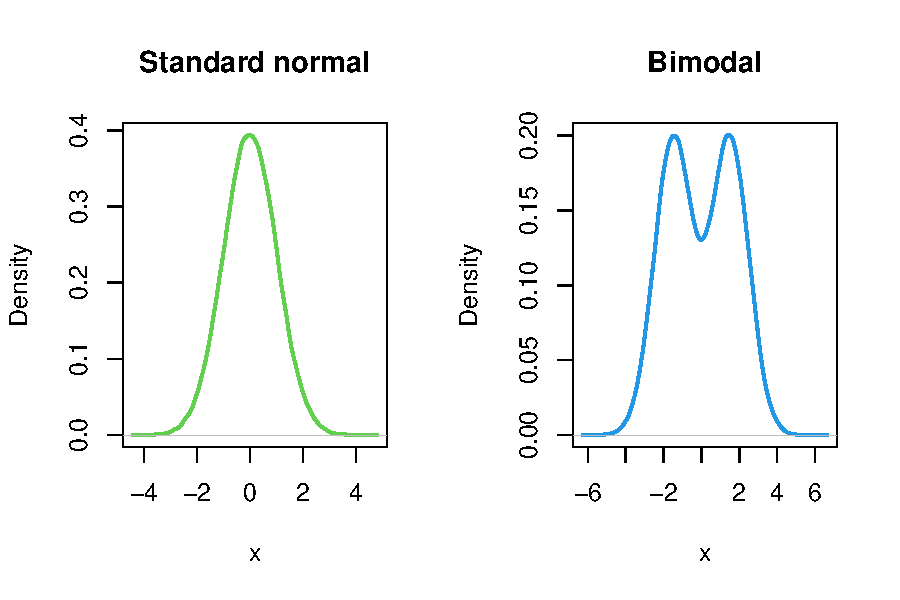
\includegraphics[width=\maxwidth]{figure/listings-unnamed-chunk-109-1} 

}

\end{Schunk}
\section{Wilkcoxon signed-rank test}\label{sec:14}
\subsection{Wilkcoxon signed-rank test}
\subsubsection{What was wrong with the sign test?}
\begin{itemize}
	\item The sign test ignores a lot of information (inefficient use of data; low power).\
	\item How can we use more information than just the sign for data with a symmetric, but possibly non-normal, distribution?
	\item Suppose the sample \( X_1,X_2,\dotsc,X_n \) are drawn from a population symmetric with respect to mean \( \mu \) (or median)
	\item We test the hypotheses: \( H_0: \mu = \mu_0 \) vs \( H_1: \mu > \mu_0 \mu < \mu_0, \mu \neq \mu_0 \).
	\item The \( t \)-test and \( Z \)-test assume a normal distribution without a long tail (outliers).
	\item They use all \textcolor{mygreen}{magnitude} information.
	\item On the other hand, the sign test discards all data information on \textcolor{mygreen}{magnitude} and hence it has low power.
\end{itemize}
\subsubsection{Ranks to the rescue}
Many non-parametric tests are based not on the data, but on their \textcolor{mygreen}{ranks}.
To find the ranks for a set od data:
\begin{itemize}
	\item Arrange the data in ascending order
	\item Assign a rank of 1 to the smallest observation, 2 to the second smallest, etc.
	\item For tied observations (in \textcolor{mygreen}{blue} or \textcolor{myred}{red} in the table below), assign each the average of the corresponding ranks
\end{itemize}
\begin{table}[H]
	\centering
	\begin{tabular}{@{}lllllllll@{}}
	\textbf{Sample}  & \textcolor{myred}{\textbf{8}} & \textcolor{mygreen}{\textbf{5}} & \textbf{10} & \textbf{2} & \textcolor{mygreen}{\textbf{5}} & \textcolor{myred}{\textbf{8}} & \textcolor{myred}{\textbf{8}} & \textbf{6}  \\
	Ordered sample   & 2 & \textcolor{mygreen}{5} & \textcolor{mygreen}{5} & 6 & \textcolor{myred}{8} & \textcolor{myred}{8} & \textcolor{myred}{8} & 10 \\
	Successive Ranks & 1 & \textcolor{mygreen}{2} & \textcolor{mygreen}{3} & 4 & \textcolor{myred}{5} & \textcolor{myred}{6} & \textcolor{myred}{7} & 8  \\
	Assigned Ranks   & 1 & \textcolor{mygreen}{2.5} & \textcolor{mygreen}{2.5} & 4 & \textcolor{myred}{6} & \textcolor{myred}{6} & \textcolor{myred}{6} & 8 
	\end{tabular}
\end{table}
\subsubsection{Thinking about magnitude}
\begin{itemize}
	\item Under the symmetric distribution assumption with mean \( \mu_0 \) from \( H_0 \), half of the \( d_i - x_i - \mu_0 \) should be negative and half positive and the expected counts are both \( \frac{n}{2} \).
	\item Under the null hypothesis, the positive and negative \( d_i \) should be of similar magnitude and occur with equal probability (on average).
	\item If we rank the absolute values of \( d_i \) in ascending order, the expected rank sums for the negative and positive \( d_i \) should be nearly equal.
\end{itemize}
\subsubsection{Wilcoxon signed-rank test}
We need to define the following quantities:
\begin{itemize}
	\item \( D_i = X_i - \mu_0 \) for \( i - 1,2,\dotsc,n \)
	\item \( R_i,\dotsc,R_n \) be the ranks of \( \lvert D_1 \rvert, \lvert D_2 \rvert, \dotsc, \lvert D_n \rvert \)
	\item \( W^+ \) be the sum of the ranks \( R_{i} \) corresponding to positive \( D_i \) 
	\item \( W^- \) be the sum of the ranks \( R_{i} \) corresponding to negative \( D_i \) 
	\item Let \( W = \min (W^+,W^-) \) 
\end{itemize}
\subsubsection{Calculations of \( w^+ \) and \( w \)}
When we observe the data we have \( d_i - x_i - \mu_0 \) with ranks (of the absolute values), \( r_1,\dotsc,r_n \) for \( \lvert d_1 \rvert, \dotsc, \lvert d_n \rvert \).
\[
	w^+ = \sum_{i: d_i > 0} r_i \quad\text{and}\quad w^- = \sum_{i: d_i < 0} r_i
\]
We should
\begin{itemize}
	\item reject \( H_0: \mu = \mu_0 \) in favour of \( H_1: \mu > \mu_0 \) if \( w^+ \) is large enough
	\item reject \( H_0: \mu = \mu_0 \) in favour of \( H_1: \mu < \mu_0 \) if \( w^+ \) is small enough
	\item reject \( H_0: \mu = \mu_0 \) in favour of \( H_1: \mu \neq \mu_0 \) if \( w^+ \) if \( w = \min(w^+,w^-) \) is small enough
\end{itemize}
Suppose \( X_i,\dotsc,X_n \) are drawn from some population that follows a symmetric distribution. Given a significance level \( \alpha \), we want to test on the population mean, \( \mu \).
\begin{redbox}{Workflow: Wikcoxon signed-rank test}
	\begin{itemize}
		\item \textbf{Hypotheses}: \( H_0: \mu = \mu_0 \) vs \( H_1: \mu > \mu_0, \mu < \mu_0 \) or \( \mu \neq \mu_0 \)
		\item \textbf{Assumptions}: \( X_i \) are independently sampled from a symmetric distribution.
		\item \textbf{Test Statistic}: \( W^+ = \sum_{i: D_i > 0} R_i \) for one-sided or \( W = \min(W^+,W^-) \) for two-sided
		\item \textbf{Observed Test Statistic}: \( w^+ \) for one-sided or \( w = \min(w^+,w^-) \) for two-sided
		\item \textbf{p-value}:
		\begin{itemize}
			\item \( P(W^+ \geq w^+) \) for \( H_1: \mu > \mu_0 \)
			\item \( P(W^+ \leq w^+) \) for \( H_1: \mu < \mu_0 \) 
			\item \( P(W^+ \leq w) \) for \( H_1: \mu \neq \mu_0 \) 
		\end{itemize}
		\item \textbf{Decision}: If the p-value is less then \( \alpha \), there is evidence against \( H_0 \). If the p-value is greater than \( \alpha \), the data are consistent with \( H_0 \).
	\end{itemize}
\end{redbox}
\subsection{Normal approximation to the wilcoxon signed-rank test statistic}
\subsubsection{Normal approximation}
For \textcolor{myred}{large enough} \( n \) we can use a normal distribution to approximate the distribution of the Wilcoxon sign rank test statistic.\\
i.e. in large samples (without ties),
\[
	W^+ \sim \mathcal{N} \left( \frac{n(N+1)}{4}, \frac{n(n+1)(2n+1)}{24} \right), \text{approximately}
\]
Hence the large sample test statistic is,
\[
	T = \frac{W^+ - \mathrm{E}(W^+)}{\sqrt{\var(W^+)}} \sim \mathcal{N}(0,1)
\]
where \( \mathrm{E}(W^+) = \frac{n(n+1)}{4} \) and \( \var(W^+) = \frac{n(n+1)(2n+1)}{24} \).  
\subsubsection{Bus Waiting Times}
The following data are waiting times for the 370 bus in minutes for 10 randomly selected passengers:
\begin{Schunk}
\begin{Sinput}
bus = c(25, 19, 9, 27, 8, 7, 26, 12, 29, 20)
\end{Sinput}
\end{Schunk}
The bus authority claims a typical wait time of 15 minutes. Do these data suggest a different typical wait time?
The standard approach is a one-sample \( t \)-test to test \( H_0: \mu = 15 \)
\begin{Schunk}
\begin{Sinput}
boxplot(bus, horizontal = TRUE, 
    	xlab = "Waiting time (mins)")
\end{Sinput}


{\centering 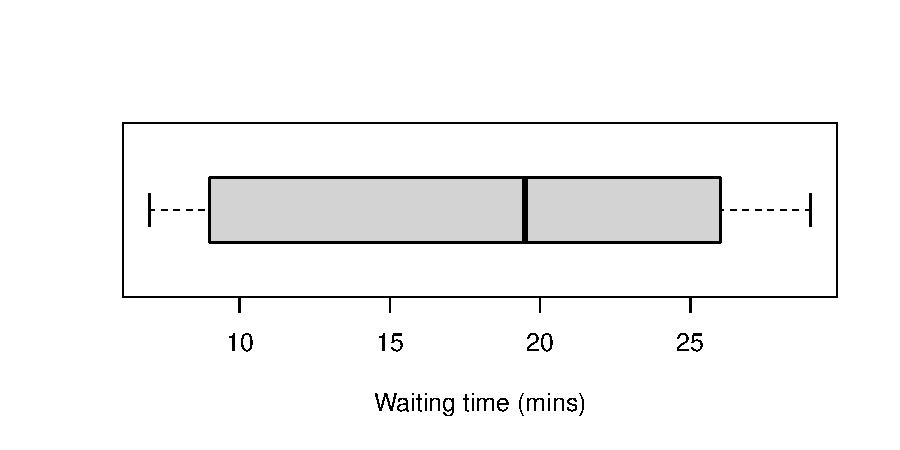
\includegraphics[width=\maxwidth]{figure/listings-unnamed-chunk-111-1} 

}

\begin{Sinput}
qqnorm(bus); qqline(bus)
\end{Sinput}


{\centering 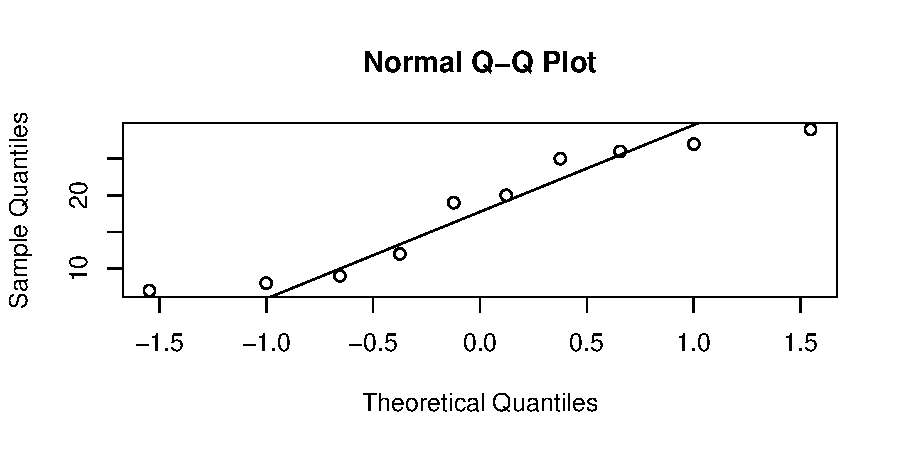
\includegraphics[width=\maxwidth]{figure/listings-unnamed-chunk-111-2} 

}

\end{Schunk}
\begin{itemize}
	\item \textbf{Hypotheses}: \( H_0: \mu = 15 \) vs \( H_1: \mu \neq 15 \)
	\item \textbf{Assumptions}: \( X_i \) are independently sampled from a symmetric distribution.
	\item \textbf{Test Statistic}: \( W = \min(W^+,W^-) \) where \( W^+ = \sum_{i:D_i>0} R_i, W^- = \sum_{i:D_i<0} R_i, D_i = X_i - 15  \)  and \( R_i \) are the ranks of \( \lvert D_1 \rvert, \lvert D_2 \rvert, \dotsc, \lvert D_n \rvert \). Under \( H_0, W^+ \sim WSR(10) \) a symmetric distribution with mean \( \mathrm{\mathrm{E}} (W^+) = \frac{n(n+1)}{4} = 27.5 \) and \( \var(W^+) = \frac{n(n+1)(2n+1)}{24} = 96.25\)  
	\item \textbf{Observed Test Statistic}: \( t:0 = \frac{w - \mathrm{E}(W^+)}{\sqrt{\var(W^+)}}  = \frac{16-27.5}{\sqrt{96.25}} = -1.172 \)
	\item \textbf{p-value}: \( 2P(W^+ \leq 16) = 0.2754 \)
	\item \textbf{Decision}: Large p-value so the data are consistent with \( H_0 \). Therefore there is no evidence to dispute the bus authority's claim of a typical wait time of 15 minutes.
\end{itemize}
\subsubsection{Normal approximation with ties}
We can approximate \( W^+ \) by a normal distribution. The p-value is approximately given by,
\begin{align*}
	\text{p-value} &\thickapprox P \left( Z \geq \frac{w^+ - \mathrm{E}(W^+)}{\sqrt{\var(W^+)}} \right) \quad\text{for}\; H_1: \mu > \mu_0\\
	\text{p-value} &\thickapprox P \left( Z \geq \frac{w^+ - \mathrm{E}(W^+)}{\sqrt{\var(W^+)}} \right) \quad\text{for}\; H_1: \mu < \mu_0\\
	\text{p-value} &\thickapprox P \left( Z \geq \left\vert\frac{w^+ - \mathrm{E}(W^+)}{\sqrt{\var(W^+)}}\right\vert \right) \quad\text{for}\; H_1: \mu \neq \mu_0,
\end{align*}
where \textcolor{myred}{\textbf{in general}}, \( \mathrm{E}(W^+) = \frac{1}{2}\sum_{i:d_i \neq 0}r_i \) and \( \var(W^+) = \frac{1}{4}\sum_{i:d_{i \neq 0}} r^{2}_{i} \).
\subsubsection{Smoking and Blood Platelets Aggregation}
	Blood samples from 11 individuals before and after they smoked a cigarette are used to measure aggregation of blood platelets.
\begin{Schunk}
\begin{Sinput}
before = c(25, 25, 27, 44, 30, 67, 53, 53, 52, 60, 28)
after =  c(27, 29, 37, 36, 46, 82, 57, 80, 61, 59, 43)
df = data.frame(before, after,
                difference = after-before)
df
\end{Sinput}
\begin{Soutput}
   before after difference
1      25    27          2
2      25    29          4
3      27    37         10
4      44    36         -8
5      30    46         16
6      67    82         15
7      53    57          4
8      53    80         27
9      52    61          9
10     60    59         -1
11     28    43         15
\end{Soutput}
\end{Schunk}
\begin{goldbox}
	Is the aggregation of blood platelets affected by smoking?
\end{goldbox}
\begin{Schunk}
\begin{Sinput}
p = df |> ggplot() +
  aes(y = "", x = difference) + 
  geom_boxplot() +
  geom_dotplot(binaxis = "x", stackdir = "center", dotsize = 0.6) +
  geom_vline(xintercept = 0, linetype='dashed') +
  labs(x = 'Difference in blood platelet levels') +
  theme_classic() +
  theme(axis.title.y=element_blank(),
        axis.text.y=element_blank(),
        axis.ticks.y=element_blank())
p
\end{Sinput}


{\centering 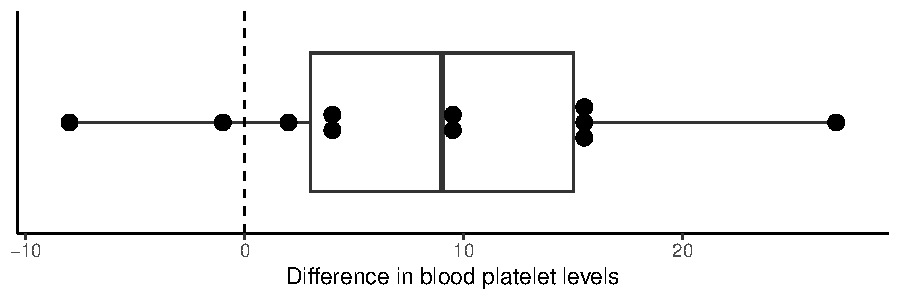
\includegraphics[width=\maxwidth]{figure/listings-unnamed-chunk-113-1} 

}

\begin{Sinput}
df = df |> dplyr::mutate(absDif = abs(difference),
                          rankAbsDif = rank(absDif),
                          srank = sign(difference)*rank(abs(difference)))
df
\end{Sinput}
\begin{Soutput}
   before after difference absDif rankAbsDif srank
1      25    27          2      2        2.0   2.0
2      25    29          4      4        3.5   3.5
3      27    37         10     10        7.0   7.0
4      44    36         -8      8        5.0  -5.0
5      30    46         16     16       10.0  10.0
6      67    82         15     15        8.5   8.5
7      53    57          4      4        3.5   3.5
8      53    80         27     27       11.0  11.0
9      52    61          9      9        6.0   6.0
10     60    59         -1      1        1.0  -1.0
11     28    43         15     15        8.5   8.5
\end{Soutput}
\begin{Sinput}
(w_p = sum(df$srank[df$srank > 0]))
\end{Sinput}
\begin{Soutput}
[1] 60
\end{Soutput}
\begin{Sinput}
(w_m = sum(-df$srank[df$srank < 0]))
\end{Sinput}
\begin{Soutput}
[1] 6
\end{Soutput}
\begin{Sinput}
(w = min(w_p, w_m))
\end{Sinput}
\begin{Soutput}
[1] 6
\end{Soutput}
\end{Schunk}
	\begin{itemize}
		\item \textbf{Hypotheses}: \( H_0: \mu_d = 0 \) vs \( H_1: \mu_d \neq 0 \)
		\item \textbf{Assumptions}: \( D_i \) are independently sampled from a symmetric distribution.
		\item \textbf{Test Statistic}: \( W+ = \sum_{i:D_i > 0} R_i \) where \( R_i \) are the ranks of \( \lvert D_1 \rvert, \lvert D_2 \rvert, \dotsc, \lvert D_n \rvert \). Under \( H_0, W^+ \sim WSR^\prime(11) \) and the set of ties as given.
		\item \textbf{Observed Test Statistic}: \( w = \min(w^+,w^-) = 6 \) because \( w^+ = 60, w^- = 6 \) 
		\item \textbf{p-value}: SInce the \( WSR^\prime(11) \) distribution is unknown, it is approximated by normal with \( E(W^+) = \frac{n(n+1)}{4} = \frac{11(11+1)}{4} = 33 \) and \( \var(W^+) = \frac{1}{4} \sum_{i=1}^{11} r^{2}_{i} = \frac{1}{4} [(2)^{2}+\dotsb+(8.5)^{2}] = \frac{506}{4} = 126.25 \). The p-value \( = 2P(W^+ \leq 6) \simeq 2P (Z \leq \frac{6-33}{\sqrt{126.25}}) = 2P(Z \leq -2.403) = 2 \times 0.008 = 0.016 \)  
		\item \textbf{Decision}: the p-value is less than 0.05, hence there is evidence against \( H_0 \).
	\end{itemize}
\begin{Schunk}
\begin{Sinput}
ew = sum(df$rankAbsDif)/2
varw = sum((df$rankAbsDif)^2)/4
c(w, ew, varw)
\end{Sinput}
\begin{Soutput}
[1]   6.00  33.00 126.25
\end{Soutput}
\begin{Sinput}
t0 = (w - ew)/sqrt(varw)
p_value = 2 * pnorm(t0)
c(t0, p_value)
\end{Sinput}
\begin{Soutput}
[1] -2.40296846  0.01626259
\end{Soutput}
\begin{Sinput}
wilcox.test(df$difference)
\end{Sinput}
\begin{Soutput}

	Wilcoxon signed rank test with continuity correction

data:  df$difference
V = 60, p-value = 0.01835
alternative hypothesis: true location is not equal to 0
\end{Soutput}
\begin{Sinput}
wilcox.test(df$difference, correct = FALSE)
\end{Sinput}
\begin{Soutput}

	Wilcoxon signed rank test

data:  df$difference
V = 60, p-value = 0.01626
alternative hypothesis: true location is not equal to 0
\end{Soutput}
\begin{Sinput}
t.test(df$difference, alternative = "two.sided")
\end{Sinput}
\begin{Soutput}

	One Sample t-test

data:  df$difference
t = 2.9065, df = 10, p-value = 0.01566
alternative hypothesis: true mean is not equal to 0
95 percent confidence interval:
  1.97332 14.93577
sample estimates:
mean of x 
 8.454545 
\end{Soutput}
\begin{Sinput}
binom.test(c(2,9), 0.5)
\end{Sinput}
\begin{Soutput}

	Exact binomial test

data:  c(2, 9)
number of successes = 2, number of trials = 11, p-value = 0.06543
alternative hypothesis: true probability of success is not equal to 0.5
95 percent confidence interval:
 0.0228312 0.5177559
sample estimates:
probability of success 
             0.1818182 
\end{Soutput}
\end{Schunk}
\subsubsection{Final notes}
A few extra notes about the Wilcoxon signed-rank test:
\begin{itemize}
	\item Since we assume that the distribution is symmetric, the hypotheses can also be stated in terms of the \textcolor{myred}{\textbf{median}} (rather than the mean).
	\item The p-value from a Wilcoxon signed-rank test will typically be smaller than the p-value of a sign test on the same data. Using the information in the ranks, the test becomes much more \textcolor{mygreen}{\textbf{powerful}} in detecting differences from \( \mu_0 \) and almost as powerful as the one sample \( t \)-test
\end{itemize}
\section{Wilcoxon rank-sum test}\label{sec:15}
\subsection{Wilcoxon rank-sum test}
It is also known as the Also known as Mann-Whitney \( U \) test or Mann-Whitney-Wilcoxon test or Wilcoxon-Mann-Whitney test
\subsubsection{Yield}
The following data yield measurements by two different methods.
\begin{Schunk}
\begin{Sinput}
A = c(32, 29, 35, 28)
B = c(27, 31, 26, 25, 30)
dat = data.frame(
	yield = c(A, B),
	method = c(rep("A", length(A)),
        	   rep("B", length(B)))
)
\end{Sinput}
\end{Schunk}
\begin{greenbox}
	\textbf{If the normality assumptions are in doubt, does the data present sufficient evidence to indicate a 	difference between method A and B?}
\end{greenbox}
\begin{Schunk}
\begin{Sinput}
ggplot(dat, aes(x = method, y = yield)) + 
geom_boxplot() + 
theme_classic() +
geom_point(colour = "#224099")
\end{Sinput}


{\centering 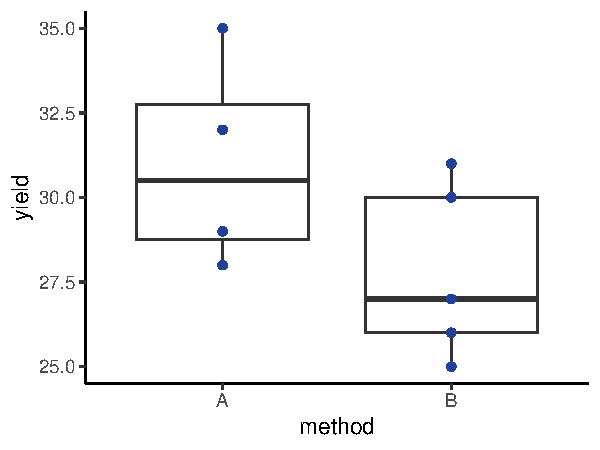
\includegraphics[width=\maxwidth]{figure/listings-unnamed-chunk-116-1} 

}

\end{Schunk}
\subsubsection{Wilcoxon rank-sum test}
\begin{itemize}
	\item A non-parametric test to compare means of two independent samples
	\item Relaxes normality assumption (like sign and Wilcoxon sign-rank tests)
	\item Also relaxes the assumption of symmetry
\end{itemize}
\subsubsection{Same same but different (location shift)}
Suppose the samples \( X_1,X_2,\dots,X_{n_x} \) and \( Y_1,Y_2,\dotsc,Y_{n_y} \) are taken from two distinct populations that follow the same kind of distribution but differ in location.
That is, \( \mu_y = \mu_x + \theta \), where \( \mu_y \) is the population mean of \( Y, \mu_x \) is the population mean of \( X \) and \( \theta \) is a \textcolor{mygreen}{\textbf{location shift}} parameter.
\begin{Schunk}
\begin{Sinput}
N = 1000
theta = 1
loc = data.frame(
obs = c(rgamma(N, 4, 4),
				rgamma(N, 4, 4)+theta),
group = rep(c("X", "Y"), each = N)
)
loc |> group_by(group) |> 
	   summarise(Mean = mean(obs),
       SD = sd(obs))
\end{Sinput}
\begin{Soutput}
# A tibble: 2 x 3
  group  Mean    SD
  <chr> <dbl> <dbl>
1 X      1.01 0.510
2 Y      1.99 0.510
\end{Soutput}
\end{Schunk}
\begin{Schunk}
\begin{Sinput}
loc |> ggplot() + 
aes(x = obs, fill = group) + 
geom_density(alpha = 0.5) +
scale_fill_manual(values=c("#992240", "#409922")) +
theme_classic()
\end{Sinput}


{\centering 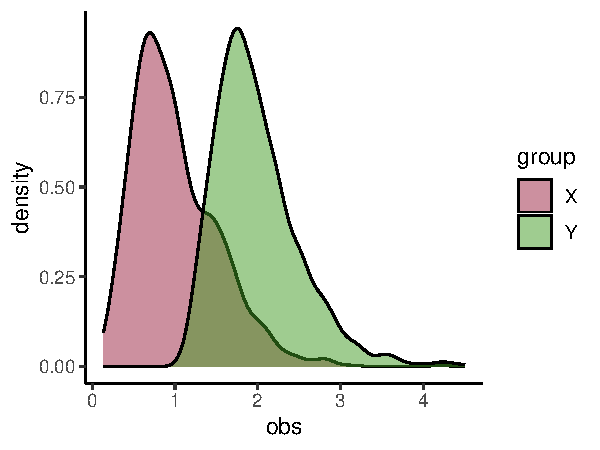
\includegraphics[width=\maxwidth]{figure/listings-unnamed-chunk-118-1} 

}

\begin{Sinput}
labs(x = "Observed values", 
	 y = "Density", 
   	 fill = "Sample")
\end{Sinput}
\begin{Soutput}
$x
[1] "Observed values"

$y
[1] "Density"

$fill
[1] "Sample"

attr(,"class")
[1] "labels"
\end{Soutput}
\end{Schunk}
\subsubsection{Wilcoxon rank-sum test}
Let \( R_1,R_2,\dots,R_N \) with \( N = n_x + n_y \) be the ranks of combined sample: \( X_1,X_2,\dotsc,X_{n_x}, Y_1,Y_2,\dots,Y_{n_Y} \)
\begin{itemize}
	\item For one sample \textcolor{myred}{\textbf{Wilcoxon signed-rank}} test, the ranks re summed over positive side of the differences
	\item For two sample \textcolor{mygreen}{\textbf{Wilcoxon rank-sum}} test, the ranks are summed over one of the samples.
	\item i.e. \( W =R_1 + R_2 + \dotsb + R_{n_X} \) 
\end{itemize}
If \( H_0 \) is true, then \( W \) should be close to its expected value
\[
	\mathrm{\mathrm{E}}=(W) = \text{Proportion} \times \text{Total rank sum} = \frac{n_x}{N} \times \frac{N(N+1)}{2} = \frac{n_x (N+1)}{2}
\]
If \( W \) is small (large), we expect \( \mu_x < \mu_y (\mu_x > \mu_y) \).
\begin{redbox}{Workflow: Wikcoxon rank-sum test}
	\begin{itemize}
		\item \textbf{Hypotheses}: \( H_0: \mu_x = \mu_y \) vs \( H_1: \mu_x > \mu_y, \mu_x < \mu_y \) or \( \mu_x \neq \mu_y \)
		\item \textbf{Assumptions}: \( X_i \) and \( Y_i \) are independent and follow the same distribution but differ by a shift.
		\item \textbf{Test Statistic}: \( W = R_1 + R_2 + \dotsb + R_{n_x} \). Under \( H_0, W \) follows the \( WRS (n_X,n_Y) \) distribution.
		\item \textbf{Observed Test Statistic}: \( w = r_1 + r_2 + \dotsb + r_{n_x} \).
		\item \textbf{p-value}: \( P(W \geq w) \) for \( H_1: \mu_x > \mu_y \) or \( P(W \leq w) \) for \( H_1: \mu_x < \mu_y \) or
		\begin{gather*}
			2P(W \geq w) \;\text{if}\; w > \frac{n_x(N+1)}{2} \;\text{and}\; H_1: \mu_x \neq \mu_y\\
			2P(W \leq w) \;\text{if}\; w < \frac{n_x(N+1)}{2} \;\text{and}\; H_1: \mu_x \neq \mu_y
		\end{gather*}
		\item \textbf{Decision}: If the p-value is less then \( \alpha \), there is evidence against \( H_0 \). If the p-value is greater than \( \alpha \), the data are consistent with \( H_0 \).
	\end{itemize}
\end{redbox}
\subsubsection{Yield example}
The following data yield measurements by two different methods.
\begin{Schunk}
\begin{Sinput}
A = c(32, 29, 35, 28)
B = c(27, 31, 26, 25, 30)
dat = data.frame(
  yield = c(A,B),
  method = c(rep("A", length(A)),
		   	 rep("B", length(B)))
)
\end{Sinput}
\end{Schunk}
If the normality assumptions are in doubt, does the data present sufficient evidence to indicate a difference in the methods A and B?
\begin{Schunk}
\begin{Sinput}
dat = dat |> mutate(rank = rank(yield))
dat
\end{Sinput}
\begin{Soutput}
  yield method rank
1    32      A    8
2    29      A    5
3    35      A    9
4    28      A    4
5    27      B    3
6    31      B    7
7    26      B    2
8    25      B    1
9    30      B    6
\end{Soutput}
\begin{Sinput}
w_A = dat |> 
filter(method == "A") |> 
pull(rank) |> 
sum()
w_A
\end{Sinput}
\begin{Soutput}
[1] 26
\end{Soutput}
\end{Schunk}
\begin{itemize}
	\item \textbf{Hypotheses}: \( H_0: \mu_x = \mu_y \)
	\item \textbf{Assumptions}: \( A_i \) and \( B_i \) are independent and follow the same distribution but differ by a shift.
	\item \textbf{Test Statistic}: \( W = R_1 + R_2 + \dotsb + R_{n_A} \). Under \( H_0, W \) follows the \( WRS (4,5) \) distribution.
	\item \textbf{Observed Test Statistic}: \( w =26 \). (sum of the ranks associated with method A).
	\item \textbf{p-value}: \( 2P(W \geq w) = 0.19 \) because \( w = 26 > \frac{n_A (N+1)}{2} = 20 \) so we're lookingin the upper tail
	\item \textbf{Decision}: As the p-value is greater than 0.05, the data are consistent with \( H_0 \).
\end{itemize}
\begin{Schunk}
\begin{Sinput}
wilcox.test(A, B) # wilcox.test(yield ~ method, data = dat)
\end{Sinput}
\begin{Soutput}

	Wilcoxon rank sum exact test

data:  A and B
W = 16, p-value = 0.1905
alternative hypothesis: true location shift is not equal to 0
\end{Soutput}
\begin{Sinput}
t.test(A, B) # t.test(yield ~ method, data = dat)
\end{Sinput}
\begin{Soutput}

	Welch Two Sample t-test

data:  A and B
t = 1.633, df = 5.8232, p-value = 0.1551
alternative hypothesis: true difference in means is not equal to 0
95 percent confidence interval:
 -1.630468  8.030468
sample estimates:
mean of x mean of y 
     31.0      27.8 
\end{Soutput}
\end{Schunk}
\subsubsection{Normal approximation}
	\begin{itemize}
		\item We can use a normal approximation to the distribution of test statistic:
		\[
			T = \frac{W - \mathrm{E}(W)}{\sqrt{\var (W)}} \sim \mathcal{N}(0,1) \;\text{approximately}
		\]
		where \( \mathrm{E}(W) = \frac{n_x (N+1)}{2} \) and \( \var (W) = \frac{n_x n_y}{N(N-1)} \left( \sum_{i=1}^{N} r_{i}^{2} - \frac{N (N+1)^2}{4} \right) \) 
		\item Our p-value calculations are:
		\begin{itemize}
			\item p-value \( \thickapprox P\left( Z \geq \frac{W-\mathrm{E}(W)}{\sqrt{\var(W)}} \right) \) for \( H_1: \mu_x > \mu_y \) 
			\item p-value \( \thickapprox P\left( Z \leq \frac{W-\mathrm{E}(W)}{\sqrt{\var(W)}} \right) \) for \( H_1: \mu_x > \mu_y \) 
			\item p-value \( \thickapprox P\left( Z \geq \left\vert \frac{W-\mathrm{E}(W)}{\sqrt{\var(W)}} \right\vert \right) \) for \( H_1: \mu_x \neq \mu_y \) 
		\end{itemize}
	\end{itemize}
\subsubsection{Latent heat of fusion}
Natrella (1963, pp. 3--23) presents data from two methods that were used in a study of the latent heat of fusion of ice. Both method A (digital method) and Method B (method of mixtures) were conducted with the specimens cooled to -0.72°C. The data represent the change in total heat from -0.72°C to water at 0°C, in calories per gram of mass.
\begin{Schunk}
\begin{Sinput}
A = c(79.98, 80.04, 80.02, 80.04, 80.03, 80.03, 80.04, 79.97, 
	80.05, 80.03, 80.02, 80.00, 80.02)
B = c(80.02, 79.94, 79.98, 79.97, 79.97, 80.03, 79.95, 79.97)
heat = data.frame(
	energy = c(A,B),
	method = rep(c("A","B"), c(length(A), length(B))))
\end{Sinput}
\end{Schunk}
\begin{goldbox}
	Does the data support the hypothesis that the electrical method (method A) gives larger results?
\end{goldbox}
\begin{Schunk}
\begin{Sinput}
heat |>
dplyr::group_by(method) |> 
dplyr::summarise(
  w = sum(r),
  xbar = mean(energy),
  s = sd(energy),
  n = n()
) |> 
knitr::kable(booktabs=TRUE, digits = 3) |>
 kable_styling(position="center", latex_options = "hold_position")
\end{Sinput}
\begin{table}[!h]
\centering
\begin{tabular}{lrrrr}
\toprule
method & w & xbar & s & n\\
\midrule
A & 2 & 80.021 & 0.024 & 13\\
B & 2 & 79.979 & 0.031 & 8\\
\bottomrule
\end{tabular}
\end{table}

\begin{Sinput}
ggplot(heat, aes(x = method, y = energy)) + 
  geom_boxplot() + 
  geom_dotplot(stackdir = "center", 
    binaxis = "y") +
  theme_linedraw() + 
  labs(y = "Heat of fusion (cal/g)",
       x = "Method")
\end{Sinput}


{\centering 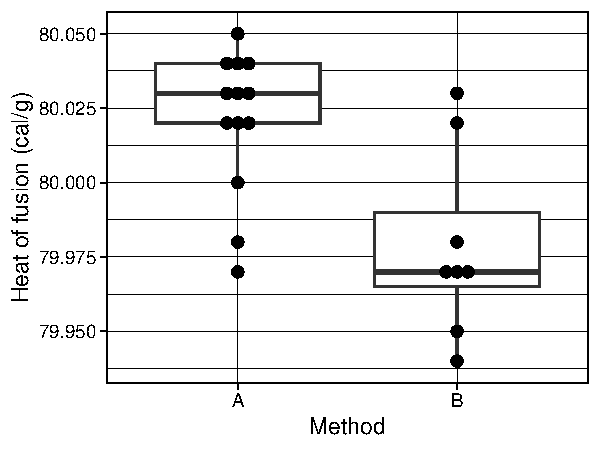
\includegraphics[width=\maxwidth]{figure/listings-unnamed-chunk-123-1} 

}

\end{Schunk}
We have \( n_A = 13, n_B = 8 \) and \( N = 21 \)
\begin{itemize}
	\item \textbf{Hypotheses}: \( H_0: \mu_x = \mu_y \)
	\item \textbf{Assumptions}: \( A_i \) and \( B_i \) are independent and follow the same distribution but differ by a shift.
	\item \textbf{Test Statistic}: \( W = R_1 + R_2 + \dotsb + R_{n_A} \). (the sum of the ranks of observations in method A). Under \( H_0, W \) follows the \( WRS^\prime (13,8) \) distribution with sizes 13, 8 and with ties as shown.
	\item \textbf{Observed Test Statistic}: \( w = r_1 + r_2 + \dotsb + r_{n_A} = 180 \).
	\item \textbf{p-value}: As the exact \( WRS^\prime (13,8) \) distribution with ties is unknown, we use a normal approximation to this distribution with \( \mathrm{E}(W) = \frac{n_x (N+1)}{2} = \frac{13\times 13 + 8 + 1}{2} = 143 \) and \( \var(W) = \frac{n_x n_y}{N(N-1)} \left( \sum_{i=1}^{N} r^{2}_{i} - \frac{N(N+1)}{4} \right) = \frac{13 (8) (3293.5-2541)}{21(20)} = 186.33 \)
	\[
		P(W \geq w) \simeq P \left( Z \geq \frac{w-\mathrm{E}(W)}{\sqrt{\var(W)}} \right) = P \left( Z \geq \frac{180 - 143}{\sqrt{186.33}} \right) = P(Z > 2.7) = 0.003
	\]
	\item \textbf{Decision}: As the p-value is greater than 0.05, the data are consistent with \( H_0 \).
\end{itemize}
\begin{Schunk}
\begin{Sinput}
wilcox.test(A, B, alternative = 'greater', correct = FALSE)
\end{Sinput}
\begin{Soutput}

	Wilcoxon rank sum test

data:  A and B
W = 89, p-value = 0.003359
alternative hypothesis: true location shift is greater than 0
\end{Soutput}
\begin{Sinput}
t.test(A, B, alternative = 'greater')
\end{Sinput}
\begin{Soutput}

	Welch Two Sample t-test

data:  A and B
t = 3.2499, df = 12.027, p-value = 0.00347
alternative hypothesis: true difference in means is greater than 0
95 percent confidence interval:
 0.01897943        Inf
sample estimates:
mean of x mean of y 
 80.02077  79.97875 
\end{Soutput}
\end{Schunk}
\subsubsection{Robustness properties}
What happens if there is an outlier in the data?
\begin{Schunk}
\begin{Sinput}
# change the first value for the B method
heat1 = heat
heat1$energy[14] = 80.20 # instead of 80.02
# recalculate ranks
heat1 = heat1 |> dplyr::mutate( 
	r = rank(energy)
)
heat1 |>
dplyr::group_by(method) |> 
dplyr::summarise(
  w = sum(r),
  Mean = mean(energy),
  SD = sd(energy),
  n = n()
) |> 
knitr::kable(digits = 3, booktabs = TRUE) |>
  kable_styling(position="center", latex_options = "hold_position")
\end{Sinput}
\begin{table}[!h]
\centering
\begin{tabular}{lrrrr}
\toprule
method & w & Mean & SD & n\\
\midrule
A & 171.5 & 80.021 & 0.024 & 13\\
B & 59.5 & 80.001 & 0.085 & 8\\
\bottomrule
\end{tabular}
\end{table}

\end{Schunk}
\begin{Schunk}
\begin{Sinput}
ggplot(heat1) + 
  aes(x = method, y = energy) + 
  geom_boxplot() + 
  theme_classic() +
  geom_dotplot(stackdir = "center",
  	binaxis = "y") +
  labs(y = "Heat of fusion (cal/g)",
    x = "Method")
\end{Sinput}


{\centering 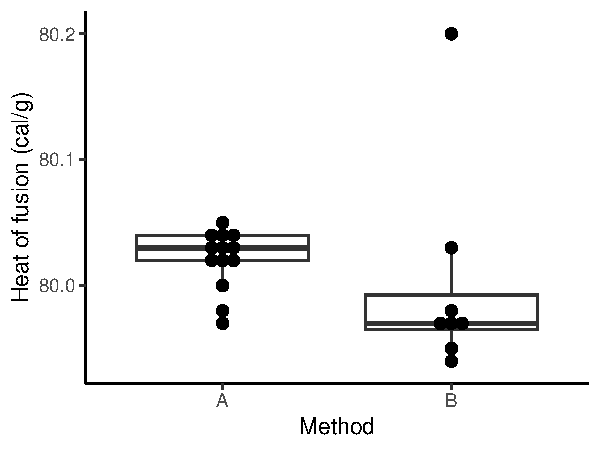
\includegraphics[width=\maxwidth]{figure/listings-unnamed-chunk-126-1} 

}

\end{Schunk}
\begin{Schunk}
\begin{Sinput}
wilcox.test(energy ~ method, data = heat1, alternative = 'greater', correct = FALSE)
\end{Sinput}
\begin{Soutput}

	Wilcoxon rank sum test

data:  energy by method
W = 80.5, p-value = 0.01859
alternative hypothesis: true location shift is greater than 0
\end{Soutput}
\end{Schunk}
\begin{Schunk}
\begin{Sinput}
t.test(energy ~ method, data = heat1, alternative = 'greater')
\end{Sinput}
\begin{Soutput}

	Welch Two Sample t-test

data:  energy by method
t = 0.63712, df = 7.6977, p-value = 0.2713
alternative hypothesis: true difference in means between group A and group B is greater than 0
95 percent confidence interval:
 -0.03774242         Inf
sample estimates:
mean in group A mean in group B 
       80.02077        80.00125 
\end{Soutput}
\end{Schunk}
\subsubsection{A heuristic for testing for differences: notched boxplot}
The upper and lower edges of the notches are at
\[
	\text{median} \pm 1.58 \times \frac{\text{IQR}}{\sqrt{n}}
\]
\textcolor{mygreen}{\textbf{Rule of thumb:}}: If the notches of two boxes do not overlap, this suggests that the medians are significantly different Mcgill et al. (1978).
\begin{Schunk}
\begin{Sinput}
ggplot(heat, aes(x = method, y = energy)) + 
geom_boxplot(notch = TRUE) + 
geom_dotplot(stackdir = "center",
	    	 binaxis = "y") +
theme_linedraw() + 
labs(y = "Heat of fusion (cal/g)",
     x = "Method")
\end{Sinput}


{\centering 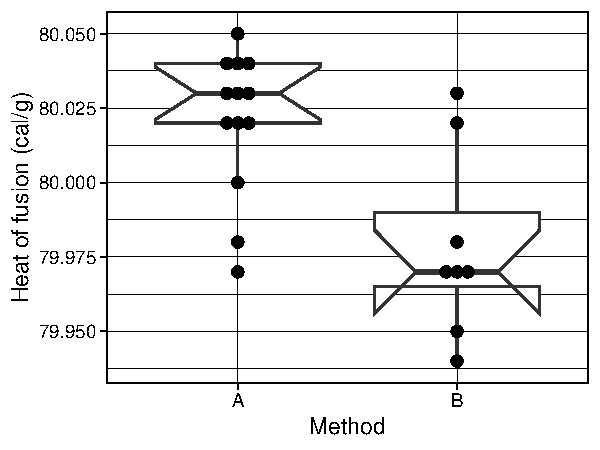
\includegraphics[width=\maxwidth]{figure/listings-unnamed-chunk-129-1} 

}

\end{Schunk}

\section{Permutation tests}\label{sec:16}
\subsection{Lady tasting tea}
\subsubsection{Lady tasting tea}
Given a cup of tea with milk, a lady claims she can discriminate as to whether milk or tea was first added to the cup.
\begin{greenbox}
	\textbf{How could we test this claim? What information would we need?}
\end{greenbox}
Fisher proposed preparing 8 cups of tea
\begin{itemize}
	\item 4 cups where tea was added before milk
	\item 4 cups where milk was added before tea
\end{itemize}
The lady would then be randomly given the cups of tea and asked to identify the 4 where tea was added before milk.\\
We would need to record:
\begin{itemize}
	\item Which cups had tea or milk added first (\textbf{truth}).
	\item Which cups the lady claimed had tea or milk added first (\textbf{predicted}).
\end{itemize}
\subsubsection{Lady tasting tea - hypothesis}
For Fisher's experiment we were left with two categorical variables.
\begin{center}
	Truth = Milk, Tea, Tea, Milk, Tea, Tea, Milk, Milk\\
	Prediction = Milk, Tea, Tea, Milk, Tea, Tea, Milk, Milk
\end{center}
Asking the question: \textbf{Are the predictions independent of the truth?} or
\[
	H_0: \text{Lady cannot take the difference vs}\; H_1: \text{Lady can taste the difference}
\]
Our \textbf{test statistic} is the number of predictions she gets correct,
\[
	T = \text{Number of tea before milk cups correctly identified}
\]
\subsubsection{Calculating significance}
The order of the cups was random, therefore there are
\[
	8! = 8 \times 7 \times 6 \times 5 \times 4 \times 3 \times 2 \times 1 = 40,320
\]
The order of the cups was random, therefore there are \( \binom{8}{4} = 70 \) ways to select which 4 cups of tea had the tea added before milk (when order doesn't matter).\\
We can look at all 70 ways and calculate how often we see a test statistic of 0,1,2,3 or 4
\begin{table}[H]
	\centering
	\begin{tabular}{@{}lccccc|l@{}}
	\toprule
	Number of correct: \( t_i \) & 0 & 1 & 2 & 3 & 4 &  \\ \midrule
	How many ways: \( f_i \) & \( \binom{4}{0} \binom{4}{4} = 1 \) & \( \binom{4}{1} \binom{4}{3} = 16 \) & \( \binom{4}{2} \binom{4}{2} = 36 \) & \( \binom{4}{1} \binom{4}{3} = 16 \) & \( \binom{4}{0} \binom{4}{4} = 1 \) & 70 \\
	Corresponding probability: \( p_i \) & \( \frac{1}{70} \) & \( \frac{16}{70} \) & \( \frac{36}{70} \) & \( \frac{16}{70} \) & \( \frac{1}{70} \) & 1 \\ \bottomrule
	\end{tabular}
\end{table}
\[
	P(\text{Getting at least 4 correct}) = P(T=4) = \frac{1}{70} = 0.014
\]
\subsubsection{Permutations}
We could also consider all 40,320 different orderings (permutations) of 8 cups of tea.
\begin{Schunk}
\begin{Sinput}
library(arrangements)
permute_8 = permutations(8)
head(permute_8, 6) # look at the "first" 6 permutations
\end{Sinput}
\begin{Soutput}
     [,1] [,2] [,3] [,4] [,5] [,6] [,7] [,8]
[1,]    1    2    3    4    5    6    7    8
[2,]    1    2    3    4    5    6    8    7
[3,]    1    2    3    4    5    7    6    8
[4,]    1    2    3    4    5    7    8    6
[5,]    1    2    3    4    5    8    6    7
[6,]    1    2    3    4    5    8    7    6
\end{Soutput}
\begin{Sinput}
tail(permute_8, 6) # look at the "last" 6 permutations
\end{Sinput}
\begin{Soutput}
         [,1] [,2] [,3] [,4] [,5] [,6] [,7] [,8]
[40315,]    8    7    6    5    4    1    2    3
[40316,]    8    7    6    5    4    1    3    2
[40317,]    8    7    6    5    4    2    1    3
[40318,]    8    7    6    5    4    2    3    1
[40319,]    8    7    6    5    4    3    1    2
[40320,]    8    7    6    5    4    3    2    1
\end{Soutput}
\end{Schunk}
If you wanted to roll your own function to calculate all possible permutations:
\begin{Schunk}
\begin{Sinput}
permutation_fn = function(n){
  if(n==1){
    return(matrix(1))
  } else {
    sp <- permutation_fn(n-1)
    p <- nrow(sp)
    A <- matrix(nrow = n*p, ncol = n)
    for(i in 1:n){
      A[(i-1)*p + 1:p, ] <- cbind(i, sp + (sp >= i))
    }
    return(A)
  }
}
\end{Sinput}
\end{Schunk}
Use the \lstinline|permutations()| function on the \lstinline|truth| vector:
\begin{Schunk}
\begin{Sinput}
truth = c("milk","tea","tea","milk","tea","tea","milk","milk")
permute_guess = permutations(truth)
permute_guess[92, ] # 92nd permutation
\end{Sinput}
\begin{Soutput}
[1] "milk" "tea"  "tea"  "milk" "milk" "milk" "tea"  "tea" 
\end{Soutput}
\end{Schunk}
	We can check if a particular sequence of tea cups is \textbf{identical} to the true sequence:
\begin{Schunk}
\begin{Sinput}
identical(truth,truth)
\end{Sinput}
\begin{Soutput}
[1] TRUE
\end{Soutput}
\begin{Sinput}
identical(permute_guess[92,], truth)
\end{Sinput}
\begin{Soutput}
[1] FALSE
\end{Soutput}
\end{Schunk}
\subsubsection{Exact p-value}
	We can calculate the exact p-value by looking across all permutations:
\begin{Schunk}
\begin{Sinput}
B = nrow(permute_guess)
check_correct = vector("numeric", length = B)
for(i in 1:B) {
  check_correct[i] = identical(permute_guess[i,], truth)
}
c(sum(check_correct), mean(check_correct))
\end{Sinput}
\begin{Soutput}
[1] 576.00000000   0.01428571
\end{Soutput}
\end{Schunk}
The p-value is the same as we get using Fisher's exact test!
\begin{Schunk}
\begin{Sinput}
truth = c("milk", "tea", "tea", "milk", "tea", "tea", "milk", "milk")
predicted = c("milk", "tea", "tea", "milk", "tea", "tea", "milk", "milk")
tea_mat = table(truth, predicted)
fisher.test(tea_mat, alternative = "greater")$p.value
\end{Sinput}
\begin{Soutput}
[1] 0.01428571
\end{Soutput}
\end{Schunk}
\subsubsection{Approximate p-value}
Often it's not feasible to consider all \( n! \) permutations, so we can \lstinline|sample()| a selection of them.
\begin{Schunk}
\begin{Sinput}
set.seed(88)
truth = c("milk","tea","tea","milk","tea","tea","milk","milk")
B = 10000
result = vector(length = B) # initialise outside the loop
for(i in 1:B){
  guess = sample(truth, size = 8, replace = FALSE) # does the permutation
  result[i] = identical(guess, truth)
}
mean(result)
\end{Sinput}
\begin{Soutput}
[1] 0.0141
\end{Soutput}
\end{Schunk}
Pretty close to the exact p-value.
\subsection{Permutation test: two independent samples}
\subsubsection{Plant growth}
The \lstinline|Plantgrowth| data has results from an experiment to compare yields (as measured by dried weight of plants) obtained under a control and two different treatment conditions (Dobson, 1983, Table 7.1).
\begin{Schunk}
\begin{Sinput}
# built into R, make it available
data("PlantGrowth") 
PlantGrowth |> ggplot() +
  aes(y = weight, x = group, 
      colour = group) + 
  geom_boxplot(coef = 10) + 
  geom_jitter(width = 0.1) + 
  theme_classic() +
  scale_colour_manual(values=c("#992240","#409922","#224099")) +
  theme(legend.position = "none") +
  labs(y = "Weight (g)", x = "Group")
\end{Sinput}


{\centering 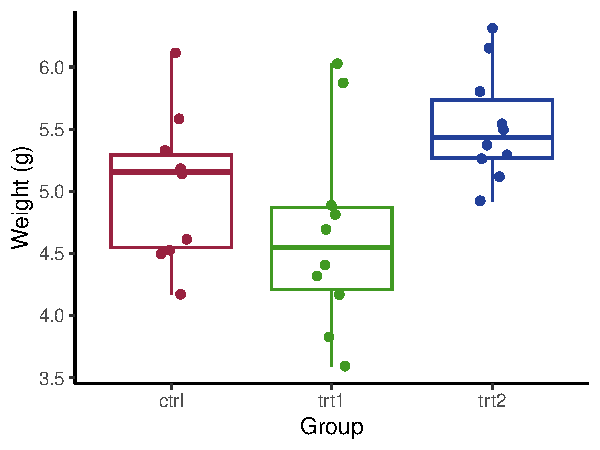
\includegraphics[width=\maxwidth]{figure/listings-unnamed-chunk-137-1} 

}

\end{Schunk}
We want to compare the \textbf{control} group to the \textbf{treatment 2} group.
\begin{Schunk}
\begin{Sinput}
dat = PlantGrowth |> filter(group %in% c("ctrl", "trt2"))
\end{Sinput}
\end{Schunk}
\subsubsection{Checking for normality: QQ plot}
\begin{Schunk}
\begin{Sinput}
dat |> 
  ggplot() + aes(sample = weight) + 
  geom_qq() + geom_qq_line() + 
  theme_classic() +
  facet_grid(cols = vars(group), labeller = label_both) + 
  labs(y = "Weight (g)", x = "Standard normal quantiles")
\end{Sinput}


{\centering 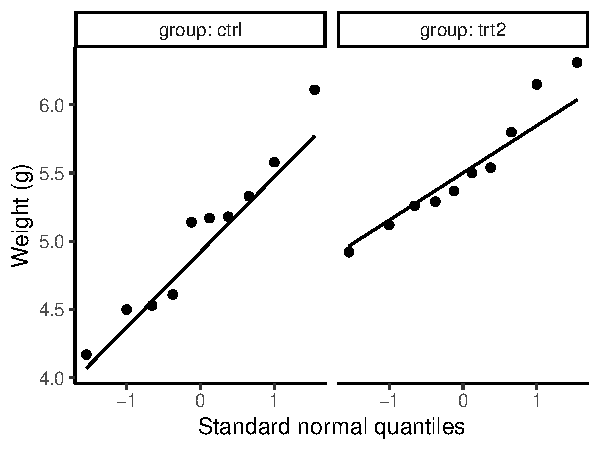
\includegraphics[width=\maxwidth]{figure/listings-unnamed-chunk-139-1} 

}

\end{Schunk}
\subsubsection{What do our ``standard'' methods say?}
\textbf{Two-sample \( t \)-test}
\begin{Schunk}
\begin{Sinput}
t.test(weight ~ group, data = dat, var.equal = TRUE)
\end{Sinput}
\begin{Soutput}

	Two Sample t-test

data:  weight by group
t = -2.134, df = 18, p-value = 0.04685
alternative hypothesis: true difference in means between group ctrl and group trt2 is not equal to 0
95 percent confidence interval:
 -0.980338117 -0.007661883
sample estimates:
mean in group ctrl mean in group trt2 
             5.032              5.526 
\end{Soutput}
\end{Schunk}
\textbf{Wilcoxon Rank-Sum Test}
\begin{Schunk}
\begin{Sinput}
wilcox.test(weight ~ group, data = dat)
\end{Sinput}
\begin{Soutput}

	Wilcoxon rank sum exact test

data:  weight by group
W = 25, p-value = 0.06301
alternative hypothesis: true location shift is not equal to 0
\end{Soutput}
\end{Schunk}
\subsubsection{Extracting information from \lstinline|t.test| objects}
\begin{Schunk}
\begin{Sinput}
tt = t.test(weight ~ group, data = dat, var.equal = TRUE)
tt
\end{Sinput}
\begin{Soutput}

	Two Sample t-test

data:  weight by group
t = -2.134, df = 18, p-value = 0.04685
alternative hypothesis: true difference in means between group ctrl and group trt2 is not equal to 0
95 percent confidence interval:
 -0.980338117 -0.007661883
sample estimates:
mean in group ctrl mean in group trt2 
             5.032              5.526 
\end{Soutput}
\begin{Sinput}
names(tt)
\end{Sinput}
\begin{Soutput}
 [1] "statistic"   "parameter"   "p.value"     "conf.int"    "estimate"   
 [6] "null.value"  "stderr"      "alternative" "method"      "data.name"  
\end{Soutput}
\begin{Sinput}
tt$statistic
\end{Sinput}
\begin{Soutput}
       t 
-2.13402 
\end{Soutput}
\end{Schunk}
\subsubsection{Permutation test}
Permute the \textcolor{myred}{\textbf{class labels}} (many times) and see what values we get for the \( t \)-test statistic
\begin{Schunk}
\begin{Sinput}
B = 10000 # number of permuted samples we will consider
permuted_dat = dat # make a copy of the data
t_null = vector("numeric", B) # initialise outside loop
for(i in 1:B) {
  permuted_dat$group = sample(dat$group) # this does the permutation
  t_null[i] = t.test(weight ~ group, data = permuted_dat)$statistic
}
\end{Sinput}
\end{Schunk}
\begin{Schunk}
\begin{Sinput}
t_null |> data.frame() |> 
  ggplot() + 
  aes(x = t_null) + 
  theme_classic() +
  geom_histogram(binwidth = 0.1) + 
  labs(
    x = "Test statistics from permuted samples"
  )
\end{Sinput}


{\centering 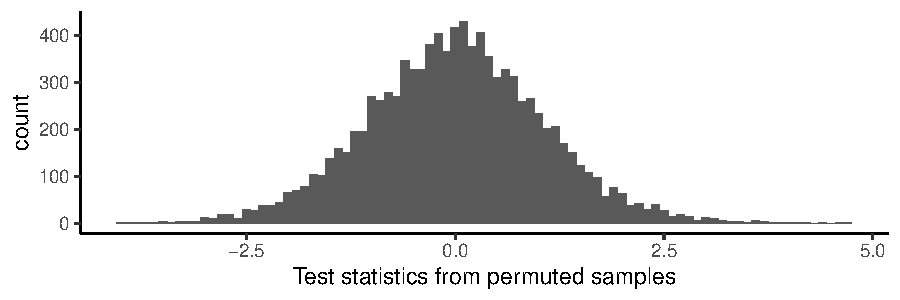
\includegraphics[width=\maxwidth]{figure/listings-unnamed-chunk-144-1} 

}

\end{Schunk}
\begin{Schunk}
\begin{Sinput}
data.frame(abs_t_null = abs(t_null)) |> 
  ggplot() + 
  aes(x = abs_t_null) +
  theme_classic() +
  geom_histogram(binwidth = 0.1,
                 boundary = 0) + 
  geom_vline(
    xintercept = abs(tt$statistic), 
    col = "#992240", lwd = 1) + 
  labs(
    x = "Absolute value of test statistic"
  )
\end{Sinput}


{\centering 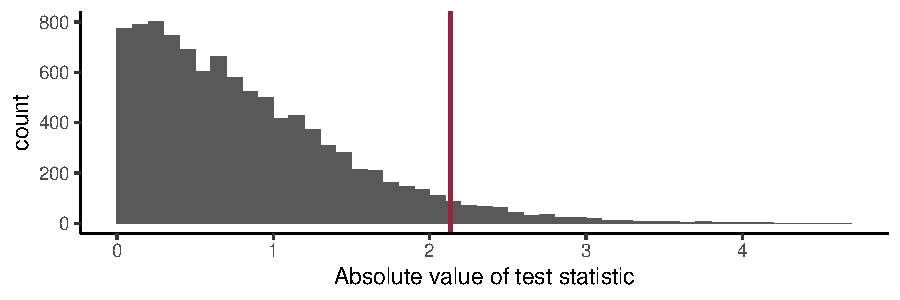
\includegraphics[width=\maxwidth]{figure/listings-unnamed-chunk-145-1} 

}

\end{Schunk}
What proportion of test statistics from randomly permuted data are more extreme than the test statistic we observed?
\begin{Schunk}
\begin{Sinput}
mean(abs(t_null) >= abs(tt$statistic))
\end{Sinput}
\begin{Soutput}
[1] 0.0501
\end{Soutput}
\end{Schunk}
This is our \textcolor{mygreen}{permutation test p-value}
\subsubsection{Permutation tests}
\begin{itemize}
	\item The two-sample \( t \)-test and the permutation test gave similar p-values, but this won't always be the case.
	\item The two-sample \( t \)-test is a \textcolor{myred}{\textbf{parametric}} test where the test statistic is assumed to follow some distribution \( (t_{n_{x}+n_{y}-2} \) distribution)
	\item The permutation test considers the \( (n_1 + n_2)! \) permutations of the labels (or a random subset to save computation time) from a single instance of the data (the \( n_1 + n_2 \) observations).
	\item The permutation test only assumes that the observations \( X_1,X_2,\dotsc,X_{n_x}, Y_1,Y_2,\dotsc,Y_{n_y} \) are \textit{exchangeable} under \( H_0 \), that is, swapping labels on observations keeps the data just as likely as the original.
	\item The permutation test may use the \( t \)-test \textcolor{mygreen}{\textbf{test statistic}} but it does not use the \( t \) \textbf{distribution}
\end{itemize}
\subsubsection{Latent heat of fusion}
Natrella (1963, pp. 3--23) presents data from two methods that were used in a study of the latent heat of fusion of ice. Both method A (digital method) and Method B (method of mixtures) were conducted with the specimens cooled to -0.72°C. The data represent the change in total heat from -0.72°C to water at 0°C, in calories per gram of mass.
\begin{greenbox}
	\textbf{Does the data support the hypothesis that the electrical method (method A) gives larger results?}
\end{greenbox}
\begin{Schunk}
\begin{Sinput}
A = c(79.98, 80.04, 80.02, 80.04, 80.03, 80.03, 80.04, 
      79.97, 80.05, 80.03, 80.02, 80.00, 80.02)
B = c(80.02, 79.94, 79.98, 79.97, 79.97, 80.03, 79.95, 
      79.97)
heat = data.frame(
  energy = c(A,B),
  method = rep(c("A","B"), c(length(A), length(B)))
)
\end{Sinput}
\end{Schunk}
\begin{Schunk}
\begin{Sinput}
heat |> ggplot() + 
  aes(x = method, y = energy) + 
  geom_boxplot(coef = 10) + 
  geom_dotplot(stackdir = "center", binaxis = "y") +
  theme_classic() +
  labs(y = "Heat of fusion (cal/g)", x = "Method")
\end{Sinput}


{\centering 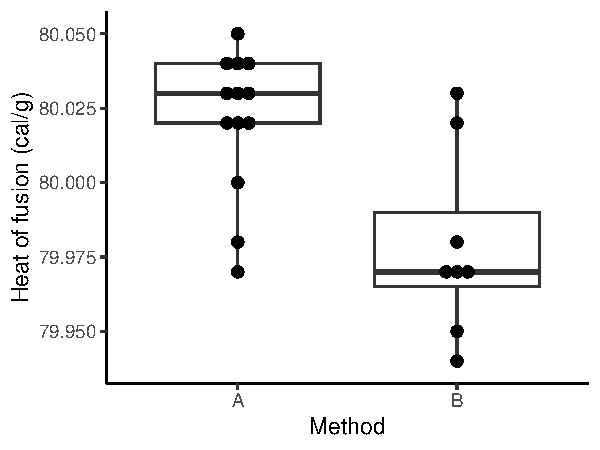
\includegraphics[width=\maxwidth]{figure/listings-unnamed-chunk-148-1} 

}

\begin{Sinput}
tt = t.test(energy ~ method, data = heat, alternative = "greater")
tt
\end{Sinput}
\begin{Soutput}

	Welch Two Sample t-test

data:  energy by method
t = 3.2499, df = 12.027, p-value = 0.00347
alternative hypothesis: true difference in means between group A and group B is greater than 0
95 percent confidence interval:
 0.01897943        Inf
sample estimates:
mean in group A mean in group B 
       80.02077        79.97875 
\end{Soutput}
\begin{Sinput}
t0_original = tt$statistic
t0_original
\end{Sinput}
\begin{Soutput}
       t 
3.249867 
\end{Soutput}
\end{Schunk}
\begin{greenbox}
	\textbf{How many permutations of the class label are there?}
\end{greenbox}
\begin{Schunk}
\begin{Sinput}
n = nrow(heat)
n
\end{Sinput}
\begin{Soutput}
[1] 21
\end{Soutput}
\begin{Sinput}
factorial(n)
\end{Sinput}
\begin{Soutput}
[1] 5.109094e+19
\end{Soutput}
\begin{Sinput}
B = 10000 # number of permuted samples we will consider
permuted_heat = heat # make a copy of the data
t_null = vector("numeric", B) # initialise outside loop
for(i in 1:B) {
  permuted_heat$method = sample(heat$method) # this does the permutation
  t_null[i] = t.test(energy ~ method, data = permuted_heat)$statistic
}
mean(t_null>=t0_original)
\end{Sinput}
\begin{Soutput}
[1] 0.0026
\end{Soutput}
\end{Schunk}
\textbf{A closer look at a few permutated samples}
\begin{Schunk}
\begin{Sinput}
perm_heat = heat 
perm_heat$id = 1
for(i in 2:6){
  temp = heat
  temp$method = sample(temp$method)
  temp$id = i
  perm_heat = rbind(perm_heat, temp)
}
perm_heat |> 
  group_by(id) |> 
  summarise(
    t_stat = t.test(
      energy[method=="A"], 
      energy[method=="B"])$statistic
  )
\end{Sinput}
\begin{Soutput}
# A tibble: 6 x 2
     id t_stat
  <dbl>  <dbl>
1     1  3.25 
2     2 -0.152
3     3  0.456
4     4 -2.14 
5     5  0.629
6     6  1.09 
\end{Soutput}
\end{Schunk}
\begin{Schunk}
\begin{Sinput}
perm_heat |> ggplot() + 
	aes(x = method, y = energy) + 
  geom_boxplot(coef = 10) + 
  theme_classic() +
  scale_y_continuous(n.breaks = 3) + 
  facet_wrap(vars(id), ncol = 6) + 
  labs(y = "Heat of fusion (cal/g)",
       x = "Method")
\end{Sinput}


{\centering 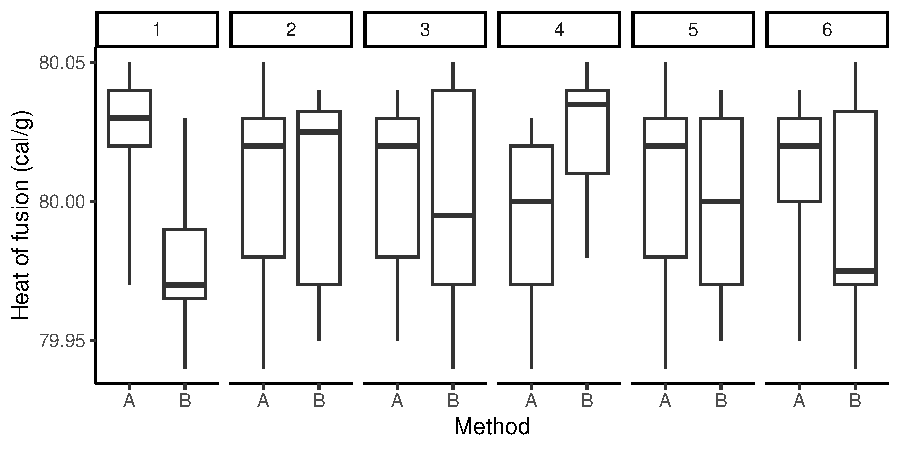
\includegraphics[width=\maxwidth]{figure/listings-unnamed-chunk-151-1} 

}

\end{Schunk}
\begin{Schunk}
\begin{Sinput}
t_null |> data.frame() |> ggplot() + 
	aes(x = t_null) +
  geom_histogram(alpha=0.5) +
  geom_vline(xintercept = t0_original, colour = "#992240", linetype = "dashed") + 
  geom_text(aes(x = t0_original, label = "Original test statistic", y = Inf), 
            colour = "#992240", angle = 90, hjust = 1, vjust = -1) + 
  theme_classic() +
  labs(x = "Test statistics from permuted samples", y = "Count")
\end{Sinput}


{\centering 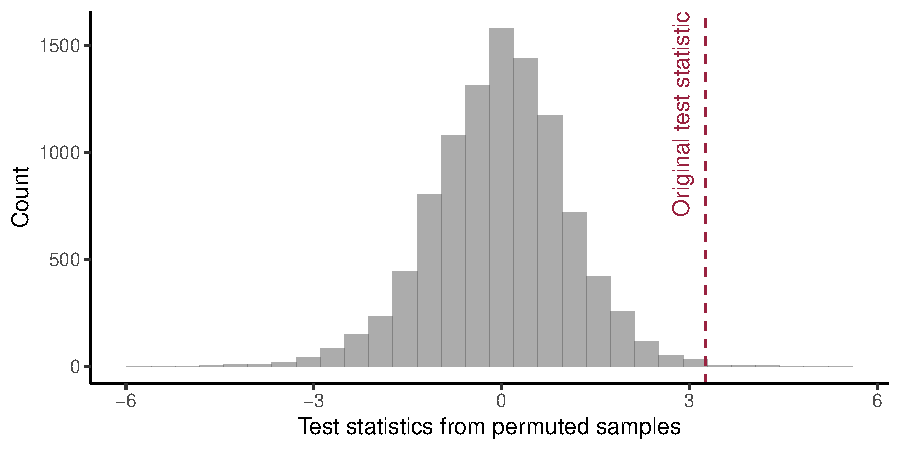
\includegraphics[width=\maxwidth]{figure/listings-unnamed-chunk-152-1} 

}

\end{Schunk}
\subsubsection{What about outliers?}
What happens if there is an outlier in the data?
Below we change the first value for the B method from 80.02 to 80.20.
\begin{Schunk}
\begin{Sinput}
heat1 = heat
heat1$energy[14]
\end{Sinput}
\begin{Soutput}
[1] 80.02
\end{Soutput}
\begin{Sinput}
# edit 80.02 -> 80.20
heat1$energy[14] = 80.20 
\end{Sinput}
\end{Schunk}
\begin{Schunk}
\begin{Sinput}
ggplot(heat1) + aes(x = method, y = energy) +
  geom_boxplot() + 
  geom_dotplot(stackdir = "center",
               binaxis = "y") +
  theme_classic() +
  labs(y = "Heat of fusion (cal/g)",
       x = "Method")
\end{Sinput}


{\centering 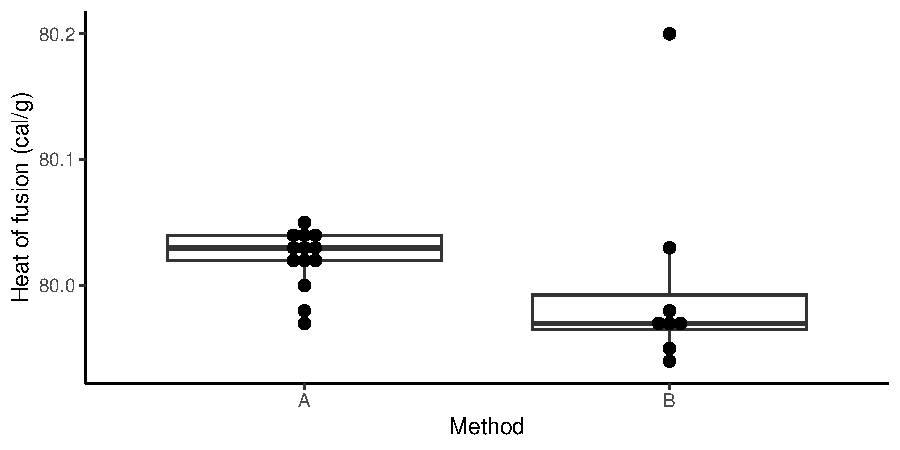
\includegraphics[width=\maxwidth]{figure/listings-unnamed-chunk-154-1} 

}

\end{Schunk}
\subsubsection{Our ``standard'' test eesults}
\textbf{Wilcoxon Rank-Sum Test}
\begin{Schunk}
\begin{Sinput}
wilcox.test(energy ~ method, data = heat1, alternative = "greater", correct = FALSE)
\end{Sinput}
\begin{Soutput}

	Wilcoxon rank sum test

data:  energy by method
W = 80.5, p-value = 0.01859
alternative hypothesis: true location shift is greater than 0
\end{Soutput}
\end{Schunk}
\textbf{Welsh Two-Sample \( t \)-test}
\begin{Schunk}
\begin{Sinput}
t.test(energy ~ method, data = heat1, alternative = "greater")
\end{Sinput}
\begin{Soutput}

	Welch Two Sample t-test

data:  energy by method
t = 0.63712, df = 7.6977, p-value = 0.2713
alternative hypothesis: true difference in means between group A and group B is greater than 0
95 percent confidence interval:
 -0.03774242         Inf
sample estimates:
mean in group A mean in group B 
       80.02077        80.00125 
\end{Soutput}
\end{Schunk}
\subsubsection{Permutation test using the Wilcoxon rank-sum statistic}
\begin{Schunk}
\begin{Sinput}
t0_original = wilcox.test(energy ~ method, data = heat1)$statistic
set.seed(88)
B = 10000
permuted_heat1 = heat1
t_null = vector("numeric", B)
for(i in 1:B){
  permuted_heat1$method = sample(heat1$method)
  t_null[i] = wilcox.test(energy ~ method, data = permuted_heat1)$statistic
}
mean(t_null >= t0_original)
\end{Sinput}
\begin{Soutput}
[1] 0.019
\end{Soutput}
\end{Schunk}
\begin{Schunk}
\begin{Sinput}
t_null |> data.frame() |> ggplot() + aes(x = t_null) +
  geom_histogram(alpha=0.5) + 
  geom_vline(xintercept = t0_original, colour = "#992240", linetype = "dashed") + 
  geom_text(aes(x = t0_original, label = "Original test statistic", y = Inf), 
            colour = "#992240", angle = 90, hjust = 1, vjust = -1) +
  theme_classic() +
  labs(x = "Test statistics from permuted samples", y = "Count")
\end{Sinput}


{\centering \includegraphics[width=\maxwidth]{figure/listings-unnamed-chunk-158-1} 

}

\end{Schunk}
\subsubsection{Robustly standardised difference in medians}
\[
	T = \frac{\widetilde{x} - \widetilde{y}}{\mathrm{MAD}(x) + \mathrm{MAD}(y)}
\]
\begin{Schunk}
\begin{Sinput}
median_a = median(heat1$energy[heat1$method=="A"])
median_b = median(heat1$energy[heat1$method=="B"])
mad_a = mad(heat1$energy[heat1$method=="A"])
mad_b = mad(heat1$energy[heat1$method=="B"])
t0_original = (median_a - median_b)/(mad_a + mad_b)

B = 10000
t_null = vector("numeric", B)
for(i in 1:B){
  permuted_heat1$method = sample(heat1$method)
  median_a = median(permuted_heat1$energy[permuted_heat1$method=="A"])
  median_b = median(permuted_heat1$energy[permuted_heat1$method=="B"])
  mad_a = mad(permuted_heat1$energy[permuted_heat1$method=="A"])
  mad_b = mad(permuted_heat1$energy[permuted_heat1$method=="B"])
  t_null[i] = (median_a - median_b)/(mad_a + mad_b)
}
mean(t_null >= t0_original)
\end{Sinput}
\begin{Soutput}
[1] 0.0165
\end{Soutput}
\end{Schunk}
\begin{Schunk}
\begin{Sinput}
t_null |> data.frame() |> ggplot() + aes(x = t_null) + 
  geom_histogram(alpha=0.5) + 
  geom_vline(xintercept = t0_original, colour = "#992240", linetype = "dashed") + 
  geom_text(aes(x = t0_original, label = "Original test statistic", y = Inf), 
            colour = "#992240", angle = 90, hjust = 1, vjust = -1) + 
  theme_classic() +
  labs(x = "Test statistics from permuted samples", y = "Count")
\end{Sinput}


{\centering \includegraphics[width=\maxwidth]{figure/listings-unnamed-chunk-160-1} 

}

\end{Schunk}
\subsection{Permutation Test: Paired Samples}
\subsubsection{Paired sample tests?}
Can we use permutation tests if we are testing for a shift in location by sampling from one population?
\begin{itemize}
	\item For paired tests we think about the differences, \( d_i = x_i - y_i \).
	\item For the Wilcoxon signed-rank test we had a test statistic involving
	\[
		\sum_{i: d_i > 0} r_i \times \mathrm{sign}(d_i)
	\]
	\item We could also think of a statistic where we used the values of the differences,
	\[
		\sum_{i=1}^{n} \lvert d_i \rvert \times \mathrm{sign}(d_i)
	\]
	\item For a permutation test permute all possible \( \mathrm{sign}(d_i) \).
\end{itemize}
\subsubsection{Smoking}
Blood samples from 11 individuals before and after they smoked a cigarette are used to measure aggregation of blood platelets.\\
Is the aggregation affected by smoking?
\begin{Schunk}
\begin{Sinput}
before = c(25, 25, 27, 44, 30, 67, 53, 53, 52, 60, 28)
after =  c(27, 29, 37, 36, 46, 82, 57, 80, 61, 59, 43)  
d = after - before
t.test(d)
\end{Sinput}
\begin{Soutput}

	One Sample t-test

data:  d
t = 2.9065, df = 10, p-value = 0.01566
alternative hypothesis: true mean is not equal to 0
95 percent confidence interval:
  1.97332 14.93577
sample estimates:
mean of x 
 8.454545 
\end{Soutput}
\end{Schunk}
There are \( 2^{11} = 2048 \) ways to permutations of sign of 11 differences.
\begin{Schunk}
\begin{Sinput}
sign_permute = permutations(c(-1,1), 11, replace = TRUE)
dim(sign_permute)
\end{Sinput}
\begin{Soutput}
[1] 2048   11
\end{Soutput}
\begin{Sinput}
head(sign_permute)
\end{Sinput}
\begin{Soutput}
     [,1] [,2] [,3] [,4] [,5] [,6] [,7] [,8] [,9] [,10] [,11]
[1,]   -1   -1   -1   -1   -1   -1   -1   -1   -1    -1    -1
[2,]   -1   -1   -1   -1   -1   -1   -1   -1   -1    -1     1
[3,]   -1   -1   -1   -1   -1   -1   -1   -1   -1     1    -1
[4,]   -1   -1   -1   -1   -1   -1   -1   -1   -1     1     1
[5,]   -1   -1   -1   -1   -1   -1   -1   -1    1    -1    -1
[6,]   -1   -1   -1   -1   -1   -1   -1   -1    1    -1     1
\end{Soutput}
\begin{Sinput}
(t0_original = mean(d)/sd(d)*sqrt(length(d)))
\end{Sinput}
\begin{Soutput}
[1] 2.906534
\end{Soutput}
\begin{Sinput}
n = length(d)
B = nrow(sign_permute)
t_null = vector("numeric", B)
for(i in 1:nrow(sign_permute)){
  d_permute = d*sign_permute[i,]
  t_null[i] = mean(d_permute)/sd(d_permute)*sqrt(n)
}
mean(abs(t_null) >= abs(t0_original))
\end{Sinput}
\begin{Soutput}
[1] 0.01660156
\end{Soutput}
\begin{Sinput}
t.test(d)$p.value
\end{Sinput}
\begin{Soutput}
[1] 0.01565739
\end{Soutput}
\end{Schunk}
\begin{Schunk}
\begin{Sinput}
t_null |> data.frame() |> ggplot() + aes(x = t_null) + 
  geom_histogram(alpha=0.5) + 
  geom_vline(xintercept = t0_original, colour = "#992240", linetype = "dashed") + 
  geom_text(aes(x = t0_original, label = "Original test statistic", y = Inf), 
            colour = "#992240", angle = 90, hjust = 1, vjust = -1) + 
  theme_classic() +
  labs(x = "Test statistics from permuted samples", y = "Count")
\end{Sinput}


{\centering \includegraphics[width=\maxwidth]{figure/listings-unnamed-chunk-163-1} 

}

\end{Schunk}
\newpage

\section{Bootstrap}\label{sec:17}
\subsection{Speed of light}
\subsubsection{Speed of light}
\begin{itemize}
	\item Simon Newcomb measured the time required for light to travel from his laboratory on the Potomac River to a mirror at the base of the Washington Monument and back, a total distance of about 7400 meters.
	\item He performed this experiment 66 times.
	\item These measurements were used to estimate the speed of light.
\end{itemize}
Newcomb's measurements of the passage time of light, made July 24, 1882 to September 5, 1882. The values \( \times^{-3} + 24.8 \) are Newcomb's measurements recorded in millionths of a second for observations of light passing over a distance of 3721 m and back, from Fort Myer on the west bank of the Potomac to a fixed mirror at the base of the Washington monument. The ``true'' value is 33.02. Stigler (1977, Table 5)
\begin{Schunk}
\begin{Sinput}
library(readr)
speed_file = read_csv("https://raw.githubusercontent.com/DATA2002/data/master/speed_of_light.txt")
speed = speed_file$Speed_of_Light
mean(speed)
\end{Sinput}
\begin{Soutput}
[1] 26.21212
\end{Soutput}
\begin{Sinput}
median(speed)
\end{Sinput}
\begin{Soutput}
[1] 27
\end{Soutput}
\end{Schunk}
\begin{Schunk}
\begin{Sinput}
library(cowplot)
p1 = ggplot(speed_file) + aes(x = "", y = Speed_of_Light) + 
  geom_boxplot(colour = "#992240", outlier.size = 4) + 
  theme_classic() +
  labs(x = "", y = "Speed") + coord_flip()
p2 = ggplot(speed_file) + aes(x = Speed_of_Light) + 
  geom_histogram(colour = "#992240") + 
  theme_classic() +
  labs(x = "Speed")
cowplot::plot_grid(p1, p2, ncol = 1, align = "v")
\end{Sinput}


{\centering \includegraphics[width=\maxwidth]{figure/listings-unnamed-chunk-165-1} 

}

\end{Schunk}
\subsection{Confidence Intervals}
\subsubsection{Estimation vs hypothesis testing}
\textbf{Estimation}
\begin{itemize}
	\item A population parameter is unknown.
	\item Use the sample statistics to generate estimates of the population parameter.
\end{itemize}
\textbf{Hypothesis Testing}
\begin{itemize}
	\item Explicit statement (or hypothesis) regarding the population parameter.
	\item Test statistics are generated which will either support or reject the null hypothesis.
\end{itemize}
\subsubsection{Confidence intervals}
\begin{itemize}
	\item We should avoid reporting just a point estimate for a sample.
	\item We should always include a measure of variability:
	\[
		\hat{\theta} \pm \text{margin of error}
	\]
	where \( \hat{\theta} \) is the point estimate (e.g. sample mean, \( \overline{X} \)).
	\item The margin of error usually takes the form
	\[
		\text{margin of error} = \text{critical value} \times \mathrm{SE}(\hat{\theta})
	\]
	where the critical value is some quantile from an appropriate distribution (e.g. \( z_{\frac{\alpha}{2}} \) or \( t_\nu(\frac{\alpha}{2}) \))  and \( \mathrm{SE}(\theta) \) is the standard error of the point estimate (e.g. \( \mathrm{SE}(\overline{X}) = \sigma / \sqrt{n} \)).
	\item The \textit{point} estimate \( \hat{\theta} \) (say \( \overline{x} \)) of a parameter \( \theta \) (say \( \mu \)) does not show its variability across samples.
	\item To show such estimation precision, we should find an \textit{interval} estimate.
\end{itemize}
\begin{bluebox}{Definition}
	Let \( \hat{\theta}_L \) and \( \hat{\theta}_R \) be two statistics. If
	\[
		P(\hat{\theta}_L \leq \theta \leq \hat{\theta}_R) = 1 - \alpha,
	\]
	then the random interval \( [\hat{\theta}_L,\hat{\theta}_R] \) is called a \( 100(1-\alpha)\% \) \textit{confidence interval} (CI) for \( \theta \), and \( 100(1-\alpha)\% \) is called the \textit{confidence level} of the interval.
\end{bluebox}
\begin{itemize}
	\item In general, the \( \alpha \) may be chosen to be 0.01, 0.05, 0.10, etc, and then we get 99\%, 95\%, 90\% confidence interval accordingly.
\end{itemize}
\subsubsection{Confidence intervals for the mean}
Let \( X_1,X_2,\dotsc,X_n \) be a random sample from normal population and \( X_i \sim \mathcal{N}(\mu,\sigma^2) \), where \( \sigma^2 \) is unknown.\\
Then \( \frac{\overline{X} - \mu}{S / \sqrt{n}} \sim t_{n-1} \) and
\begin{align*}
	P \left( -c < \frac{\overline{X} - \mu}{S / \sqrt{n}} < c \right) &= 1 - \alpha\\
	P \left(-\frac{cS}{\sqrt{n}} < \mu - \overline{X} < \frac{cS}{\sqrt{n}}\right) &= 1-\alpha\\
	P \left(\overline{X} - \frac{cS}{\sqrt{n}} < \mu < \overline{X} + \frac{cS}{\sqrt{n}} \right) &= 1-\alpha
\end{align*}
\subsubsection{Meaning of the confidence interval}
Suppose a 95\% confidence interval for the mean \( \mu \) is \( (a,b) \).
\begin{itemize}
	\item This \textcolor{myred}{does \textbf{not}} mean that 95\% of the means \( \mu \) are in \( (a,b) \), that is \( P(a < \mu < b) = 0.95 \) since \( \mu \) is a \textbf{fixed} but unknown parameter.
	\item It also \textcolor{myred}{does \textbf{not}} mean \( P(a < \overline{X} < b) = 0.95 \), where \( \overline{X} \) is the sample mean since the CI is for the true mean \( \mu \) not the sample mean \( \overline{X} \).
\end{itemize}
It \textcolor{myred}{\textbf{\textbf{does}}} mean that if we draw a large number of random samples and compute for each sample a 95\% CI, about 95\% of these CIs will contain \( \mu \).
It \textbf{can} be described as a \textcolor{mygreen}{\textbf{range of possible values}} for the population parameter.
\subsubsection{Confidence intervals}
A confidence interval is a statement about the underlying population parameter.
\begin{itemize}
	\item Formally, for a 95\% confidence interval, 95\% of all possible random samples will contain the population mean, leading to 95\% \textcolor{myred}{\textbf{confidence}} that a single interval contains the true mean.
	\item In reality, a specific interval either contains the mean or it doesn't. We just do not know which one is true; but we have 95\% \textcolor{myred}{\textbf{confidence}} that it does.
\end{itemize}
In this context \textcolor{myred}{\textbf{confidence}} isn't the same as \textcolor{mygreen}{\textbf{probability}}.
\subsubsection{Distributional assumptions}
\begin{greenbox}
	\textbf{What happens if your data does not follow a normal distribution?}
\end{greenbox}
\begin{enumerate}
	\item Guess the distribution of the data and use this distribution to calculate critical values for confidence levels. \textcolor{myred}{\textbf{Risky}}.
	\item Use \textcolor{mygreen}{\textbf{bootstrap resampling}} to empirically model the distribution of the data.
\end{enumerate}
\subsection{Bootstrapping}
\subsubsection{Bootstrapping resampling}
Bootstrapping is a computational process that allows us to as make inferences about the population where no information is available about the population.
Bootstrap methods take their name from the idea of ``lifting yourself up by your bootstraps'' - moving up without any additional outside help. The name was introduced by Efron (1979).
\begin{quote}
	``in the absence of any other knowledge about a population, the distribution of values found in a sample of size n from the population is the best guide to the distribution in the population. Therefore, to approximate what would happen if the population was resampled it is sensible to resample the sample.'' Manly (2007, p. 41)
\end{quote}
The classic approach to bootstrapping is to \textcolor{mygreen}{\textbf{repeatedly resample}} from the sample (with replacement).
\subsubsection{Speed of light}
\begin{itemize}
	\item Simon Newcomb measured the time required for light to travel from his laboratory on the Potomac River to a mirror at the base of the Washington Monument and back, a total distance of about 7400 meters.
	\item He performed this experiment 66 times (66 observations).
	\item These measurements were used to estimate the speed of light.
	\item What if we approximated \textbf{sampling from the population} by \textbf{sampling from this sample\textbf{}}?
\end{itemize}
\subsubsection{Bootstrapping speed of light measurements}
\begin{Schunk}
\begin{Sinput}
mean(speed)
\end{Sinput}
\begin{Soutput}
[1] 26.21212
\end{Soutput}
\begin{Sinput}
set.seed(88)
B = 10000
result = vector("numeric", length = B)
for(i in 1:B){
  newData = sample(speed, replace = TRUE)
  result[i] = mean(newData)
}
round(head(result), 2)
\end{Sinput}
\begin{Soutput}
[1] 22.98 26.15 27.38 24.67 26.11 25.20
\end{Soutput}
\begin{Sinput}
hist(result, col = "#224099")
\end{Sinput}


{\centering \includegraphics[width=\maxwidth]{figure/listings-unnamed-chunk-166-1} 

}

\end{Schunk}
\subsubsection{Bootstrap confidence intervals}
Efron (1979) proposed that the bootstrap confidence interval be the quantiles from the bootstrap distribution.
In general, \( (\theta_L^\ast, \theta_U^\ast) \) are the bounds of the \( 100(1-\alpha) \) bootstrap CI where \( \theta_L^\ast \) is the \( \frac{\alpha}{2} \) quantile from the bootstrap distribution and  \( \theta_U^\ast \) is the \( 1-\frac{\alpha}{2} \) quantile from the bootstrap distribution.\\
If \lstinline|result| has our bootstrap estimates then we can get a 95\% confidence interval using:
\begin{Schunk}
\begin{Sinput}
quantile(result, c(0.025, 0.975))
\end{Sinput}
\begin{Soutput}
    2.5%    97.5% 
23.36364 28.37917 
\end{Soutput}
\end{Schunk}
\subsubsection{Speed of light}
\begin{Schunk}
\begin{Sinput}
CI = quantile(result, c(0.025, 0.975))
CI
\end{Sinput}
\begin{Soutput}
    2.5%    97.5% 
23.36364 28.37917 
\end{Soutput}
\begin{Sinput}
CI - mean(speed)
\end{Sinput}
\begin{Soutput}
     2.5%     97.5% 
-2.848485  2.167045 
\end{Soutput}
\begin{Sinput}
hist(result, breaks = 50,
     col = "#224099")
abline(v = CI, col = "#992240", lwd = 2)
\end{Sinput}


{\centering \includegraphics[width=\maxwidth]{figure/listings-unnamed-chunk-168-1} 

}

\end{Schunk}
Compare with the confidence interval using the \( t \) distribution.
\begin{Schunk}
\begin{Sinput}
xbar = mean(speed)
n = length(speed)
se = sd(speed)/sqrt(n)
c(xbar, n, se)
\end{Sinput}
\begin{Soutput}
[1] 26.212121 66.000000  1.322658
\end{Soutput}
\begin{Sinput}
critical_values = qt(c(0.025,0.975), 
                     df = n-1)
critical_values
\end{Sinput}
\begin{Soutput}
[1] -1.997138  1.997138
\end{Soutput}
\begin{Sinput}
CI_t = xbar + critical_values*se
CI_t
\end{Sinput}
\begin{Soutput}
[1] 23.57059 28.85365
\end{Soutput}
\begin{Sinput}
hist(result, breaks = 50,
     col = "#224099")
abline(v = CI, col = "#992240", lwd = 2)
abline(v = CI_t, col = "#409922", 
       lwd = 2, lty = 2)
\end{Sinput}


{\centering \includegraphics[width=\maxwidth]{figure/listings-unnamed-chunk-169-1} 

}

\end{Schunk}
\subsubsection{What if we trimmed the data?}
\begin{Schunk}
\begin{Sinput}
hist(speed, col = "#224099", 
     breaks = 15)
\end{Sinput}


{\centering \includegraphics[width=\maxwidth]{figure/listings-unnamed-chunk-170-1} 

}

\end{Schunk}
Keep only the positive speeds.
\begin{Schunk}
\begin{Sinput}
speed1 = speed[speed>0]
mean(speed)
\end{Sinput}
\begin{Soutput}
[1] 26.21212
\end{Soutput}
\begin{Sinput}
mean(speed1)
\end{Sinput}
\begin{Soutput}
[1] 27.75
\end{Soutput}
\end{Schunk}
\subsubsection{Speed of light}
\begin{Schunk}
\begin{Sinput}
B = 10000
result = vector("numeric", length = B)
for(i in 1:B){
  newData = sample(speed1, replace = TRUE)
  result[i] = mean(newData)
}
CI = quantile(result, c(0.025, 0.975))
CI
\end{Sinput}
\begin{Soutput}
    2.5%    97.5% 
26.50000 28.96875 
\end{Soutput}
\begin{Sinput}
CI - mean(speed1)
\end{Sinput}
\begin{Soutput}
    2.5%    97.5% 
-1.25000  1.21875 
\end{Soutput}
\begin{Sinput}
hist(result, breaks = 50, col = "#224099")
abline(v = CI, col = "#992240", lwd = 2)
\end{Sinput}


{\centering \includegraphics[width=\maxwidth]{figure/listings-unnamed-chunk-172-1} 

}

\end{Schunk}
Much more symmetric.
Compare with the confidence interval using the \( t \) distribution.
\begin{Schunk}
\begin{Sinput}
xbar = mean(speed1)
n = length(speed1)
se = sd(speed1)/sqrt(n)
c(xbar, n, se)
\end{Sinput}
\begin{Soutput}
[1] 27.7500000 64.0000000  0.6354289
\end{Soutput}
\begin{Sinput}
critical_values = qt(c(0.025,0.975), df = n-1)
critical_values
\end{Sinput}
\begin{Soutput}
[1] -1.998341  1.998341
\end{Soutput}
\begin{Sinput}
CI_t = xbar + critical_values*se
CI_t
\end{Sinput}
\begin{Soutput}
[1] 26.4802 29.0198
\end{Soutput}
\begin{Sinput}
hist(result, breaks = 50,
     col = "#224099")
abline(v = CI, col = "#992240", lwd = 2)
abline(v = CI_t, col = "#409922", 
       lwd = 2, lty = 2)
\end{Sinput}


{\centering \includegraphics[width=\maxwidth]{figure/listings-unnamed-chunk-173-1} 

}

\end{Schunk}
\subsection{Example: flight departure delays}
\subsubsection{Flights data set}
\begin{Schunk}
\begin{Sinput}
library(nycflights13)
glimpse(flights)
\end{Sinput}
\begin{Soutput}
Rows: 336,776
Columns: 19
$ year           <int> 2013, 2013, 2013, 2013, 2013, 2013, 2013, 2013, 2013, 2~
$ month          <int> 1, 1, 1, 1, 1, 1, 1, 1, 1, 1, 1, 1, 1, 1, 1, 1, 1, 1, 1~
$ day            <int> 1, 1, 1, 1, 1, 1, 1, 1, 1, 1, 1, 1, 1, 1, 1, 1, 1, 1, 1~
$ dep_time       <int> 517, 533, 542, 544, 554, 554, 555, 557, 557, 558, 558, ~
$ sched_dep_time <int> 515, 529, 540, 545, 600, 558, 600, 600, 600, 600, 600, ~
$ dep_delay      <dbl> 2, 4, 2, -1, -6, -4, -5, -3, -3, -2, -2, -2, -2, -2, -1~
$ arr_time       <int> 830, 850, 923, 1004, 812, 740, 913, 709, 838, 753, 849,~
$ sched_arr_time <int> 819, 830, 850, 1022, 837, 728, 854, 723, 846, 745, 851,~
$ arr_delay      <dbl> 11, 20, 33, -18, -25, 12, 19, -14, -8, 8, -2, -3, 7, -1~
$ carrier        <chr> "UA", "UA", "AA", "B6", "DL", "UA", "B6", "EV", "B6", "~
$ flight         <int> 1545, 1714, 1141, 725, 461, 1696, 507, 5708, 79, 301, 4~
$ tailnum        <chr> "N14228", "N24211", "N619AA", "N804JB", "N668DN", "N394~
$ origin         <chr> "EWR", "LGA", "JFK", "JFK", "LGA", "EWR", "EWR", "LGA",~
$ dest           <chr> "IAH", "IAH", "MIA", "BQN", "ATL", "ORD", "FLL", "IAD",~
$ air_time       <dbl> 227, 227, 160, 183, 116, 150, 158, 53, 140, 138, 149, 1~
$ distance       <dbl> 1400, 1416, 1089, 1576, 762, 719, 1065, 229, 944, 733, ~
$ hour           <dbl> 5, 5, 5, 5, 6, 5, 6, 6, 6, 6, 6, 6, 6, 6, 6, 5, 6, 6, 6~
$ minute         <dbl> 15, 29, 40, 45, 0, 58, 0, 0, 0, 0, 0, 0, 0, 0, 0, 59, 0~
$ time_hour      <dttm> 2013-01-01 05:00:00, 2013-01-01 05:00:00, 2013-01-01 0~
\end{Soutput}
\end{Schunk}
\subsubsection{New York City to San Fransisco}
Let's restrict attention to flights between NYC and San Francisco (SFO).
\begin{Schunk}
\begin{Sinput}
sfo = flights |> filter(dest == "SFO")
\end{Sinput}
\end{Schunk}
This is the \textbf{population} of flights in 2013. Let's look at the distribution of arrival delays:
\begin{Schunk}
\begin{Sinput}
sfo |> ggplot() + aes(x = arr_delay/60) +
  geom_histogram() + 
  theme_classic() +
  labs(x = "Arrival delay (hours)")
\end{Sinput}
\begin{Soutput}
Warning: Removed 158 rows containing non-finite values (`stat_bin()`).
\end{Soutput}


{\centering \includegraphics[width=\maxwidth]{figure/listings-unnamed-chunk-176-1} 

}

\end{Schunk}
\subsubsection{Travel policy}
An organisation regularly flies staff from NYC to SFO. It decides that it is acceptable for staff to be late 2\% of the time. How early should they book their flights to ensure that staff arrive on time?
\begin{Schunk}
\begin{Sinput}
quantile(sfo$arr_delay, p = 0.98, na.rm = TRUE)
\end{Sinput}
\begin{Soutput}
98% 
153 
\end{Soutput}
\end{Schunk}
The 98th percentile of the arrival delay distribution is about 2.5 hours, so we should send them on a flight about 2.5 hours early.
\begin{greenbox}
	\textbf{What if we didn't have the population data?}
\end{greenbox}
\subsubsection{Sample of flights}
If all we had access to was a sample of 100 flights from 2013, this is our point estimate of the 98th percentile.
\begin{Schunk}
\begin{Sinput}
set.seed(88)
sfo_sample = sfo |> filter(!is.na(arr_delay)) |> sample_n(size = 100, replace = FALSE)
quantile(sfo_sample$arr_delay, p = 0.98)
\end{Sinput}
\begin{Soutput}
  98% 
94.72 
\end{Soutput}
\end{Schunk}
\begin{greenbox}
	\textbf{How reliable is that point estimate?}
\end{greenbox}
\subsubsection{Bootstrap CI for quantiles}
\begin{Schunk}
\begin{Sinput}
B = 10000
q98 = vector("numeric", length = B)
for(i in 1:B) {
  resample = sample(sfo_sample$arr_delay, 
                    replace = TRUE)
  q98[i] = quantile(resample, probs = 0.98)
}
hist(q98, col = "#224099")
\end{Sinput}


{\centering \includegraphics[width=\maxwidth]{figure/listings-unnamed-chunk-179-1} 

}

\end{Schunk}
A 95\% confidence interval for this quantile:
\begin{Schunk}
\begin{Sinput}
quantile(q98, c(0.025,0.975))
\end{Sinput}
\begin{Soutput}
 2.5% 97.5% 
 38.6 182.0 
\end{Soutput}
\end{Schunk}
Based on our sample our (bootstrap) 95\% confidence interval is between 1 hour and 3 hours.
\subsubsection{Final remarks}
Bootstrapping is useful when
\begin{itemize}
	\item the theoretical distribution of a statistic is complicated or unknown (e.g. coefficient of variation, quantile regression parameter estimates, etc.)
	\item the sample size is too small to make any sensible parametric inferences about the parameter
\end{itemize}
\textbf{Advantages}
\begin{itemize}
	\item Bootstrapping frees us from making parametric assumptions to carry out inferences
	\item Provides answers to problems for which analytic solutions are impossible
	\item Can be used to verify, or check the stability of results
	\item Asymptotically consistent
\end{itemize}
\section{Linear Models}\label{sec:18}
\subsection{One Sample}
\subsubsection{Beer contents}
Beer contents in a pack of six bottles (in millilitres) are:
\begin{Schunk}
\begin{Sinput}
y = c(374.8, 375.0, 375.3, 374.8, 374.4, 374.9)
\end{Sinput}
\end{Schunk}
Is the mean beer content less than the 375 mL claimed on the label?
\begin{Schunk}
\begin{Sinput}
df = data.frame(y)
set.seed(124)
ggplot(df, aes(x = "", y = y)) +
  geom_boxplot(alpha = 0.5, coef = 10) + 
  geom_dotplot(binaxis = 'y', 
               stackdir = 'center') + 
  geom_hline(yintercept = 375, 
             colour = "blue",
             linetype = "dashed") + 
  labs(y = "Beer volume (ml)", x = "") +
  theme_bw() + 
  theme(axis.ticks.x = element_blank(),
        axis.text.x = element_blank())
\end{Sinput}


{\centering \includegraphics[width=\maxwidth]{figure/listings-unnamed-chunk-182-1} 

}

\end{Schunk}
\subsubsection{Beer contents: one sample \( t \)-test}
\begin{Schunk}
\begin{Sinput}
t.test(df$y, mu = 375)
\end{Sinput}
\begin{Soutput}

	One Sample t-test

data:  df$y
t = -1.1094, df = 5, p-value = 0.3177
alternative hypothesis: true mean is not equal to 375
95 percent confidence interval:
 374.5577 375.1756
sample estimates:
mean of x 
 374.8667 
\end{Soutput}
\end{Schunk}
Linear model:
\[
	Y = \beta_0 + \varepsilon
\]
\begin{Schunk}
\begin{Sinput}
beer_lm = lm(y~1, data = df)
confint(beer_lm)
\end{Sinput}
\begin{Soutput}
               2.5 %   97.5 %
(Intercept) 374.5577 375.1756
\end{Soutput}
\end{Schunk}
Or alternatively:
\[
	(Y -\mu_0) = \beta_0 + \beta_1 x + \varepsilon
\]
\begin{Schunk}
\begin{Sinput}
beer_lm0 = lm(y-375 ~ 1, data = df)
summary(beer_lm0)$coefficients |> round(4)
\end{Sinput}
\begin{Soutput}
            Estimate Std. Error t value Pr(>|t|)
(Intercept)  -0.1333     0.1202 -1.1094   0.3177
\end{Soutput}
\end{Schunk}
\subsubsection{Beer contents: Wilcoxon signed-rank test}
\begin{Schunk}
\begin{Sinput}
wilcox.test(df$y, mu = 375, exact = FALSE)
\end{Sinput}
\begin{Soutput}

	Wilcoxon signed rank test with continuity correction

data:  df$y
V = 4, p-value = 0.4164
alternative hypothesis: true location is not equal to 375
\end{Soutput}
\end{Schunk}
Define a function that converts the data to signed-ranks:
\begin{Schunk}
\begin{Sinput}
signed_rank = function(x) sign(x)*rank(abs(x))
\end{Sinput}
\end{Schunk}
Linear model:
\[
	\mathrm{signed\_rank}(Y -\mu_0) = \beta_0 + \beta_1 x + \varepsilon
\]
\begin{Schunk}
\begin{Sinput}
beer_lm = lm(signed_rank(y-375) ~ 1, data = df)
summary(beer_lm)$coefficients %>% round(3)
\end{Sinput}
\begin{Soutput}
            Estimate Std. Error t value Pr(>|t|)
(Intercept)   -1.667      1.558   -1.07    0.334
\end{Soutput}
\end{Schunk}
Not exact, but ballpark similar p-value. The approximation gets better as the sample size increases.\\
Let's generate a larger sample to see if the approximation works.
\begin{Schunk}
\begin{Sinput}
set.seed(88)
y_new = rnorm(n = 25, 
              mean = mean(y),
              sd = sd(y))
wilcox.test(y_new, mu = 375)
\end{Sinput}
\begin{Soutput}

	Wilcoxon signed rank exact test

data:  y_new
V = 90, p-value = 0.05158
alternative hypothesis: true location is not equal to 375
\end{Soutput}
\end{Schunk}
Linear model:
\[
	\mathrm{signed\_rank}(Y -\mu_0) = \beta_0 + \beta_1 x + \varepsilon
\]
\begin{Schunk}
\begin{Sinput}
beer_lm = lm(signed_rank(y_new - 375) ~ 1)
summary(beer_lm)$coefficients |> round(4)
\end{Sinput}
\begin{Soutput}
            Estimate Std. Error t value Pr(>|t|)
(Intercept)     -5.8      2.794 -2.0758   0.0488
\end{Soutput}
\end{Schunk}
That's a closer approximate p-value.
\subsection{Two Sample}
\subsubsection{Latent Heat of Fusion}
Two methods labelled A and B are used to measure the latent heat of fusion of ice. Does the data support the assumption that A gives larger results?
\begin{Schunk}
\begin{Sinput}
A = c(79.98, 80.04, 80.02, 80.04, 80.03, 80.03, 80.04, 
      79.97, 80.05, 80.03, 80.02, 80.00, 80.02)
B = c(80.02, 79.94, 79.98, 79.97, 79.97, 80.03, 79.95, 
      79.97)
heat = data.frame(
  energy = c(A,B),
  method = rep(c("A","B"), c(length(A), length(B)))
)
heat = heat |> dplyr::mutate(
  r = rank(energy)
)
heat |> ggplot() + 
  aes(x = method, y = energy) + 
  geom_point(alpha = 0.5) +
  theme_classic()
\end{Sinput}


{\centering \includegraphics[width=\maxwidth]{figure/listings-unnamed-chunk-191-1} 

}

\end{Schunk}
Recode \lstinline|A| as \lstinline|0| and \lstinline|B| as \lstinline|1|:
\begin{Schunk}
\begin{Sinput}
heat = heat |> mutate(
  method_dummy = if_else(
    method == "A", 0, 1))
heat |> ggplot() +
  aes(x = method_dummy, 
      y = energy) + 
  geom_point(alpha = 0.5) + 
  geom_smooth(method = "lm",
              se = FALSE) + 
  scale_x_continuous(breaks = c(0,1)) +
  theme_classic()
\end{Sinput}


{\centering \includegraphics[width=\maxwidth]{figure/listings-unnamed-chunk-192-1} 

}

\end{Schunk}
\subsubsection{Latent heat of fusion: two-sample \( t \)-test}
\begin{Schunk}
\begin{Sinput}
tt = t.test(
  energy ~ method,
  data = heat, 
  var.equal = TRUE)
tt$statistic |> round(4)
\end{Sinput}
\begin{Soutput}
     t 
3.4722 
\end{Soutput}
\begin{Sinput}
tt$p.value |> round(4)
\end{Sinput}
\begin{Soutput}
[1] 0.0026
\end{Soutput}
\begin{Sinput}
tt$conf.int |> round(3)
\end{Sinput}
\begin{Soutput}
[1] 0.017 0.067
attr(,"conf.level")
[1] 0.95
\end{Soutput}
\end{Schunk}
Linear model:
\[
	Y = \beta_0 + \beta_1 x + \varepsilon
\]
\begin{Schunk}
\begin{Sinput}
heat_lm = lm(energy ~ method, data = heat)
summary(heat_lm)$coefficients |> round(4)
\end{Sinput}
\begin{Soutput}
            Estimate Std. Error    t value Pr(>|t|)
(Intercept)  80.0208     0.0075 10713.4567   0.0000
methodB      -0.0420     0.0121    -3.4722   0.0026
\end{Soutput}
\begin{Sinput}
confint(heat_lm) |> round(3)
\end{Sinput}
\begin{Soutput}
             2.5 % 97.5 %
(Intercept) 80.005 80.036
methodB     -0.067 -0.017
\end{Soutput}
\begin{Sinput}
c(tt$est, unname(diff(tt$est))) |> round(4)
\end{Sinput}
\begin{Soutput}
mean in group A mean in group B                 
        80.0208         79.9788         -0.0420 
\end{Soutput}
\end{Schunk}
\subsubsection{Latent heat of fusion: ranks}
\begin{Schunk}
\begin{Sinput}
heat |> ggplot() +
  aes(x = method, y = rank(energy)) + 
  geom_point(alpha = 0.5) +
  theme_classic()
\end{Sinput}


{\centering \includegraphics[width=\maxwidth]{figure/listings-unnamed-chunk-195-1} 

}

\begin{Sinput}
heat |> ggplot() +
  aes(x = method_dummy, 
      y = rank(energy)) + 
  geom_point(alpha = 0.5) + 
  geom_smooth(method = "lm",
              se = FALSE) +
  theme_classic()
\end{Sinput}


{\centering \includegraphics[width=\maxwidth]{figure/listings-unnamed-chunk-195-2} 

}

\end{Schunk}
\subsubsection{Latent heat of fusion: Wilcoxon rank-sum test}
\begin{Schunk}
\begin{Sinput}
wilcox.test(energy ~ method, data = heat)$p.value
\end{Sinput}
\begin{Soutput}
Warning in wilcox.test.default(x = DATA[[1L]], y = DATA[[2L]], ...): cannot compute exact p-value with ties
\end{Soutput}
\begin{Soutput}
[1] 0.007497146
\end{Soutput}
\end{Schunk}
Linear model:
\[
	\text{rank}(Y) = \beta_0 + \beta_1 x + \varepsilon
\]
\begin{Schunk}
\begin{Sinput}
heat_lm = lm(rank(energy) ~ method, data = heat)
summary(heat_lm)$coefficients |> round(3)
\end{Sinput}
\begin{Soutput}
            Estimate Std. Error t value Pr(>|t|)
(Intercept)   13.846      1.388   9.973    0.000
methodB       -7.471      2.249  -3.322    0.004
\end{Soutput}
\end{Schunk}
\newpage

\section{Multiple Testing}\label{sec:19}
\subsection{microRNA and Alzheimer's Disease}
\subsubsection{microRNA and Alzheimer's Disease}
MicroRNA are small non-coding RNA molecules that regulate gene expression.
\begin{greenbox}
	\textbf{Is there any evidence that microRNA behaviour in the brain might be associated with Alzheimer's disease? (Patrick et al., 2017)}
\end{greenbox}
\begin{itemize}
	\item Experiment by measuring the amount of 309 microRNAs in 701 subjects.
	\item Test for significant differences between the means of subjects with and without Alzheimer's disease for each microRNA.
\end{itemize}
\subsubsection{What does this microRNA data look like?}
We start with a \lstinline|RData| file that has two objects in it: \lstinline|AD| and \lstinline|microRNA_Data|.
\begin{Schunk}
\begin{Sinput}
load("data/microRNA_full.RData")
\end{Sinput}
\end{Schunk}
The \lstinline|AD| object is a named vector where the names correspond to the subject (person) and the values correspond to the presence or absence of Alzheimer's disease.
\begin{Schunk}
\begin{Sinput}
str(AD)
\end{Sinput}
\begin{Soutput}
 Named int [1:701] 1 0 1 1 1 1 0 0 1 1 ...
 - attr(*, "names")= chr [1:701] "20264936" "50105725" "20730959" "11229148" ...
\end{Soutput}
\begin{Sinput}
head(AD)
\end{Sinput}
\begin{Soutput}
20264936 50105725 20730959 11229148 20151388 11259716 
       1        0        1        1        1        1 
\end{Soutput}
\end{Schunk}
Convert this to a data frame and move the names into their own column:
\begin{Schunk}
\begin{Sinput}
disease_status = data.frame(AD) |> 
  tibble::rownames_to_column("subject")
str(disease_status)
\end{Sinput}
\begin{Soutput}
'data.frame':	701 obs. of  2 variables:
 $ subject: chr  "20264936" "50105725" "20730959" "11229148" ...
 $ AD     : int  1 0 1 1 1 1 0 0 1 1 ...
\end{Soutput}
\end{Schunk}
The measurements are in the \lstinline|microRNA_Data| object where columns are subjects and rows are the miRNAs.
\begin{Schunk}
\begin{Sinput}
microRNA_Data[1:4,1:3]
\end{Sinput}
\begin{Soutput}
           20264936 50105725 20730959
hsa-let-7a 11.97670 12.61142 13.34787
hsa-let-7b 12.24761 11.77856 11.44760
hsa-let-7c 11.07564 11.68883 11.79726
hsa-let-7d 11.30709 11.50804 11.37125
\end{Soutput}
\end{Schunk}
Reshape the microRNA data and merge in the disease status information:
\begin{Schunk}
\begin{Sinput}
mirna = microRNA_Data |>
  tibble::rownames_to_column("microRNA") |> 
  tidyr::pivot_longer(cols = -1, names_to = "subject", values_to = "value") |> 
  dplyr::left_join(disease_status)
head(mirna, n = 4)
\end{Sinput}
\begin{Soutput}
# A tibble: 4 x 4
  microRNA   subject  value    AD
  <chr>      <chr>    <dbl> <int>
1 hsa-let-7a 20264936  12.0     1
2 hsa-let-7a 50105725  12.6     0
3 hsa-let-7a 20730959  13.3     1
4 hsa-let-7a 11229148  12.5     1
\end{Soutput}
\end{Schunk}
How many patients have Alzheimer's?
\begin{Schunk}
\begin{Sinput}
library(janitor)
mirna |> select(subject, AD) |> 
  distinct() |> 
  janitor::tabyl(AD) |> 
  janitor::adorn_pct_formatting()
\end{Sinput}
\begin{Soutput}
 AD   n percent
  0 273   38.9%
  1 428   61.1%
\end{Soutput}
\end{Schunk}
\begin{Schunk}
\begin{Sinput}
mirna |> 
  group_by(microRNA) |> 
  nest() |> 
  ungroup() |> 
  slice(1:15) |> # extract first 15 groups
  unnest(cols = everything()) |> 
  ggplot() + 
  aes(y = reorder(microRNA, value), 
      x = value, colour = factor(AD)) + 
  geom_boxplot(coef = 10) + 
  scale_color_manual(values=c("#992240", "#224099")) + 
  theme_classic() +
  theme(legend.position = "top") + 
  labs(colour = "Disease status",
       y = "MicroRNA")
\end{Sinput}


{\centering \includegraphics[width=\maxwidth]{figure/listings-unnamed-chunk-204-1} 

}

\end{Schunk}
\subsubsection{Lots of \( t \)-tests}
Let's use Welch two-sample t-tests to compare the mean for people with Alzheimer's to people without Alzheimer's for all 309 microRNA.
\begin{Schunk}
\begin{Sinput}
mirna_res = mirna |> 
  group_by(microRNA) |> 
  summarise(pval = t.test(value~AD)$p.value)
mirna_res |> ggplot() + aes(x = pval) + 
  theme_classic() +
  geom_histogram(boundary = 0, binwidth = 0.05, 
                 fill = "skyblue",
                 colour = "black")
\end{Sinput}


{\centering \includegraphics[width=\maxwidth]{figure/listings-unnamed-chunk-205-1} 

}

\begin{Sinput}
sum(mirna_res$pval < 0.05)
\end{Sinput}
\begin{Soutput}
[1] 49
\end{Soutput}
\end{Schunk}
Of the 309 microRNA tested, 49 have p-values less than 0.05.
\begin{greenbox}
	\textbf{Are all of these ``statistically significant'' differences important?}
\end{greenbox}
\subsubsection{Lots of \( t \)-tests when \( H_0 \) is TRUE}
\begin{itemize}
	\item If there was \textbf{no association} between any microRNAs and Alzheimer's disease our p-values follow a uniform distribution.
	\item We can generate a set of p-values \textit{knowing} that there is no association and visualise this.
\end{itemize}
\begin{Schunk}
\begin{Sinput}
set.seed(88)
mirna_res = mirna_res |> 
  mutate(null_pval = runif(n = n(), 
                           min = 0, 
                           max = 1))
mirna_res |> ggplot() + aes(x = null_pval) + 
  theme_classic() +
  geom_histogram(boundary = 0, 
                 binwidth = 0.05,
                 fill = "#224099", 
                 colour = "black")
\end{Sinput}


{\centering \includegraphics[width=\maxwidth]{figure/listings-unnamed-chunk-206-1} 

}

\begin{Sinput}
sum(mirna_res$null_pval < 0.05)
\end{Sinput}
\begin{Soutput}
[1] 17
\end{Soutput}
\end{Schunk}
When we \textbf{know} that there are no truly important microRNAs, we still see 15 ``significant'' p-values in this simulated example.
\subsubsection{The Reality of the Situation}
\begin{itemize}
	\item We never really know what is a real association.
	\item A small p-value provides some evidence against the null bit it could still be a false positive.
	\item Type 1 error \( (\alpha = 0.05) \) 
\end{itemize}
\begin{goldbox}
	For every model we evaluate at \( \alpha = 0.05 \), we accept that there is a 5\% chance that we \textcolor{myred}{reject the null hypothesis} when \textcolor{mygreen}{the null hypothesis is actually true}.
\end{goldbox}
\subsubsection{Types of Errors}
Suppose you are testing a hypothesis that a parameter \( \theta \) equals zero versus the alternative that it does not equal zero.
\begin{itemize}
	\item \textbf{Type I error or false positive} \( (V) \)\\
	Conclude that \( \theta \) does not equal zero when it does.
	\item \textbf{Type II error or false negative} \( (T) \)\\
	Conclude that \( \theta \) equals zero when it doesn't.
\end{itemize}
Possible outcomes from a series of \( m \) hypothesis tests.
\begin{table}[H]
	\centering
	\begin{tabular}{@{}lccc@{}}
	\toprule
	Outcomes                        & Truth \( \theta = 0 \) & Truth \( \theta \neq 0 \) & Number of tests \\ \midrule
	Conclusion: \( \theta = 0 \)    & \( U \)                & \( T \)                   & \( m - R \)     \\
	Conclusion: \( \theta \neq 0 \) & \( V \)                & \( S \)                   & \( R \)         \\
	Number of tests                 & \( m_0 \)              & \( m - m_0 \)             & \( m \)         \\ \bottomrule
	\end{tabular}
\end{table}
\subsubsection{Error Rates}
\textcolor{myred}{\textbf{False positive rate}}: the rate at which null results \( (\theta = 0) \) are called significant,
\[
	\mathrm{E} \left[ \frac{V}{m_0} \right]
\]
\textcolor{myred}{\textbf{Family wise error rate (FWER)}}: the probability of at least one false positive,
\[
	P(V \geq 1)
\]
\textcolor{myred}{\textbf{False discovery rate (FDR)}}: the rate at which claims of significance are false,
\[
	\mathrm{E} \left[ \frac{V}{R} \right]
\]
\subsubsection{Accounting for Multiple Testing}
\begin{itemize}
	\item If p-values  are correctly calculated calling all p-values less than \( \alpha \) significant will control the false positive rate at level \( \alpha \), on average.
	\item You perform 10,000 tests and the reality is that \( \theta = 0 \) for all of them.
	\begin{greenbox}
		\textbf{In what sort of situation might you be doing 10,000 hypothesis tests?}
	\end{greenbox}
	\item Suppose that you call all p-values less than 0.05 significant.
	\item The expected number of false positives is: \( 10,000 \times 0.05 = 500 \) false positives 
	\begin{greenbox}
		\textbf{How do we avoid so many false positives?}
		\begin{itemize}
			\item Control the \textcolor{mygreen}{\textbf{Family-Wise Error Rate (FWER)}}
			\item Control the \textcolor{myred}{\textbf{False Discovery Rate (FDR)}}
		\end{itemize}
	\end{greenbox}
\end{itemize}
\subsection{Controlling the Family-Wise Error Rate}
\subsubsection{Family-Wise Error Rate}
\textcolor{myred}{\textbf{Family-Wise Error Rate (FWER)}}: the probability of at least one false positive.\\
Let \( T_1,\dotsc,T_m \) be \( m \) test statistics for null hypothesis \( H_{01},\dotsc,H_{0m} \).\\
The FWER is the probability of falsely rejecting one or more \( H_{0i} \),
\[
	\mathrm{FWER} = P(V \geq 1).
\]
If the \textbf{null hypothesis is always true} but we conduct \( m \) tests each significance level \( \alpha \) then\dots
\begin{itemize}
	\item The probability of at least one false positive is \( 1 - (1 - \alpha)^m \)
	\item e.g. if \( m = 20 \) then the FWER is \( 64\% \) 
\end{itemize}
\begin{Schunk}
\begin{Sinput}
m = 20
alpha = 0.05
1 - (1 - alpha)^m
\end{Sinput}
\begin{Soutput}
[1] 0.6415141
\end{Soutput}
\end{Schunk}
\subsubsection{Bonferroni Correction}
The \textcolor{myred}{Bonferroni correction} is the oldest multiple testing correction.
Given that the number of false positives for \( m \) tests is \( m \alpha \) then consider defining a new threshold for significance:
\[
	\alpha^\ast = \frac{\alpha}{m}
\]
\begin{itemize}
	\item This is ``conservative'' but keeps FWER \( \leq \alpha \) 
	\item For \( m = 20 \),
	\[
		1 - (1 - \alpha^\ast)^m = 1 - (1 - \frac{0.05}{20})^{20} \thickapprox 0.0488.
	\]
\end{itemize}
\begin{Schunk}
\begin{Sinput}
m = 20
alpha = 0.05
1 - (1 - alpha/m)^m
\end{Sinput}
\begin{Soutput}
[1] 0.04883012
\end{Soutput}
\end{Schunk}
\textbf{Basic Idea}
\begin{itemize}
	\item Suppose you do \( m \) tests
	\item You want to control FWER at level \( \alpha \) so \( P(V \geq 1) \leq \alpha \)
	\begin{itemize}
		\item That is, the probability of making one or more type I errors is controlled at level \( \alpha \).
	\end{itemize}
	\item Calculate p-values in the usual way
	\item Set \( \alpha^\ast = \frac{\alpha}{m} \) (or alternatively calculate adjusted p-values: \( p^\ast = \text{p-value} \times m \))
	\item Call all p-values less than \( \alpha^\ast \) significant (or all adjusted p-values less than \( \alpha \) significant)
\end{itemize}
\textbf{Pros}: Easy to calculate, conservative\\
\textbf{Cons}: May be very ``conservative''
\subsubsection{10 microRNA p-values: Bonferroni Method}
For the sake of illustration, we're going to control the error rates at \( \alpha = 0.2 \). Let's also say that we are only interested in \( m = 10 \) of the microRNA.
\begin{Schunk}
\begin{Sinput}
alpha = 0.2
m = 10
M = nrow(mirna_res)
set.seed(88, sample.kind = "Rounding")
\end{Sinput}
\begin{Soutput}
Warning in set.seed(88, sample.kind = "Rounding"): non-uniform 'Rounding' sampler used
\end{Soutput}
\begin{Sinput}
sample_rows = sample(1:M, size = m)
mirna10 = mirna_res |> 
  select(microRNA, pval) |> 
  slice(sample_rows) |> 
  mutate(p_bonferroni = pmin(pval*m, 1)) |> 
  arrange(pval)
\end{Sinput}
\end{Schunk}
We compare the original p-values to \( \frac{0.2}{m} = 0.02 \) or the adjusted p-values \lstinline|p_bonferroni| to \( \alpha = 0.02 \). We get the same conclusion either way.
\begin{Schunk}
\begin{Sinput}
mirna10 |> 
  knitr::kable(digits = 4, booktabs=TRUE) |>
    kable_styling(position="center", latex_options = "hold_position")
\end{Sinput}
\begin{table}[!h]
\centering
\begin{tabular}{lrr}
\toprule
microRNA & pval & p\_bonferroni\\
\midrule
hsv1-miR-H3 & 0.0785 & 0.7851\\
hsv1-miR-H8 & 0.2251 & 1.0000\\
hsa-miR-451 & 0.2308 & 1.0000\\
hsa-miR-518e & 0.2590 & 1.0000\\
hsa-miR-30c & 0.2842 & 1.0000\\
\addlinespace
hsa-miR-222 & 0.4863 & 1.0000\\
hsa-let-7a & 0.5538 & 1.0000\\
hsa-miR-92b & 0.7672 & 1.0000\\
hsa-miR-124 & 0.7698 & 1.0000\\
hsa-miR-516a-3p & 0.9980 & 1.0000\\
\bottomrule
\end{tabular}
\end{table}

\end{Schunk}
\subsection{Controlling the False Discovery Rate}
\subsubsection{False Discovery Rate}
Aim: to keep the expected proportion of false positives in your rejected tests (FDR) close to \( \alpha \)
Let
\begin{itemize}
	\item \( R = \) total number of \( H_{0i} \) rejected
	\item \( V = \) number of \( H_{0i} \) falsely rejected
	\item FRD \( = \mathrm{E}\left( \frac{V}{R} \right) \) 
\end{itemize}
\subsubsection{Controlling False Discovery Rate (FDR)}
The \textcolor{myred}{Benjamini--Hochberg} procedure is the most popular correction when performing \textit{lots} of tests say in genomics, imaging, astronomy, or other signal-processing disciplines.
\textbf{Basic idea}:
	\begin{itemize}
		\item Suppose you do \( m \) tests and want to \textbf{control FDR} at level \( \alpha \)
		\item Calculate p-values normally
		\item Order the p-values from smallest to largest \( p_{(1)} \leq p_{(2)} \leq \dotsb \leq p_{(m)} \)
		\item Find \( j^\ast = \max j \) such that \( p_{(j)} \leq \frac{j}{m} \alpha \)
		\item Reject all \( H_{0i} \) where \( p_{(i)} \leq \frac{j^\ast}{m} \alpha \)
	\end{itemize}
\textbf{Pros}: Still pretty easy to calculate, less conservative (maybe much less)\\
\textbf{Cons}: Allows for more false positives, may behave strangely under dependence
\subsubsection{10 microRNA p-values: BH method}
Controlling the FDR rates at \( \alpha = 0.2 \) . Take a the same sample of 10 p-values from the microRNA experiment.
\begin{Schunk}
\begin{Sinput}
alpha = 0.2
m = 10
p_vals = sort(mirna10$pval)
# BH procedure
# j=1: smallest p-value < 1*alpha/m?
p_vals[1] < 1*alpha/m
\end{Sinput}
\begin{Soutput}
[1] FALSE
\end{Soutput}
\begin{Sinput}
# j=2: 
# second smallest p-value < 2*alpha/m?
p_vals[2] < 2*alpha/m
\end{Sinput}
\begin{Soutput}
[1] FALSE
\end{Soutput}
\begin{Sinput}
# j=3: 
# third smallest p-value < 3*alpha/m?
p_vals[3] < 3*alpha/m
\end{Sinput}
\begin{Soutput}
[1] FALSE
\end{Soutput}
\begin{Sinput}
# j=4: 
# fourth smallest p-value < 4*alpha/m?
p_vals[4] < 4*alpha/m
\end{Sinput}
\begin{Soutput}
[1] FALSE
\end{Soutput}
\begin{Sinput}
# j=5: 
# fifth smallest p-value < 5*alpha/m?
p_vals[5] < 5*alpha/m
\end{Sinput}
\begin{Soutput}
[1] FALSE
\end{Soutput}
\begin{Sinput}
# and so on ...
\end{Sinput}
\end{Schunk}
\subsubsection{10 microRNA p-values: BH vs Bonferonni}
Controlling all error rates at \( \alpha = 0.20 \) and using our sample of 10 microRNAs.\\
The lines are the significance thresholds for the three methods. If a point is below the line, the method would consider it ``significant''.
\begin{Schunk}
\begin{Sinput}
alpha = 0.2; m = 10
pvaldf = data.frame(p_vals) |> mutate(rank = rank(p_vals, ties.method = "random"))
pvaldf |> ggplot() + aes(y = p_vals, x = rank) + 
  geom_abline(aes(intercept = 0, slope=alpha*1/m, colour = 'Benjamini–Hochberg (FDR)'), linewidth = 1.5) +
  geom_hline(aes(yintercept = alpha, colour = 'No correction'), linewidth = 1.5) + 
  geom_hline(aes(yintercept = alpha/m, colour = 'Bonferroni (FWER)'), linewidth = 1.5) + 
  geom_point(size = 2) + 
  scale_x_continuous(breaks = 1:10) + 
  scale_colour_manual(name='Method',
                     breaks=c('No correction', 'Bonferroni (FWER)', 'Benjamini–Hochberg (FDR)'),
                     values=c('No correction'='#224099',
                              'Bonferroni (FWER)'='#992240', 
                              'Benjamini–Hochberg (FDR)'='#409922')) +
  theme_classic() + 
  labs(y = "p-value", x = "Ordering")
\end{Sinput}


{\centering \includegraphics[width=\maxwidth]{figure/listings-unnamed-chunk-212-1} 

}

\end{Schunk}
\subsection{Simulation Experiments}
\subsubsection{Case Study I: No True Positives}
\begin{Schunk}
\begin{Sinput}
set.seed(88)
p_vals = rep(NA, 1000)
B = 10000
case1 = tibble(experiment = 1:B) |> 
  group_by(experiment) |> 
  summarise(x_sample = rnorm(20),
            y_sample = rnorm(20)) |> 
  nest() |> 
  mutate(
    test = map(data, 
               ~t.test(.$x_sample, 
                       .$y_sample,
                       var.equal = TRUE) |> 
                 broom::tidy())) |> 
  unnest(test) |> 
  ungroup()
mean(case1$p.value < 0.05)
\end{Sinput}
\begin{Soutput}
[1] 0.0501
\end{Soutput}
\begin{Sinput}
case1 |> ggplot() + aes(x = p.value) + 
  theme_classic() +
  geom_histogram(boundary = 0, binwidth = 0.05, 
                 fill = "#224099", colour = "black")
\end{Sinput}


{\centering \includegraphics[width=\maxwidth]{figure/listings-unnamed-chunk-213-1} 

}

\end{Schunk}
Get R to do the corrections for us using the \lstinline|p.adjust()| function:
\begin{Schunk}
\begin{Sinput}
case1 = case1 |> 
  mutate(
    p_bonf = p.adjust(p.value, 
                      "bonferroni"),
    p_bh = p.adjust(p.value, "BH")
  )
case1 |> select(experiment, p.value,
                 p_bonf, p_bh) |> 
  head()
\end{Sinput}
\begin{Soutput}
# A tibble: 6 x 4
  experiment p.value p_bonf  p_bh
       <int>   <dbl>  <dbl> <dbl>
1          1   0.612      1 0.989
2          2   0.385      1 0.989
3          3   0.310      1 0.989
4          4   0.126      1 0.989
5          5   0.385      1 0.989
6          6   0.710      1 0.989
\end{Soutput}
\end{Schunk}
Proportion of ``significant'' results
\begin{Schunk}
\begin{Sinput}
case1 |> ungroup() |> 
  summarise(
    original = mean(p.value < 0.05),
    bonferroni = mean(p_bonf < 0.05),
    bh = mean(p_bh < 0.05)
  )
\end{Sinput}
\begin{Soutput}
# A tibble: 1 x 3
  original bonferroni    bh
     <dbl>      <dbl> <dbl>
1   0.0501          0     0
\end{Soutput}
\end{Schunk}
\subsubsection{Case study II: 50\% true positives}
\begin{Schunk}
\begin{Sinput}
set.seed(88)
B = 10000
case2 = tibble(experiment = 1:B) |> 
  group_by(experiment) |> 
  summarise(x_sample = rnorm(20), y_sample = rnorm(20)) |> 
  rowwise() |> 
  mutate(truth = if_else(experiment<=B/2, "mu1 - mu2 = 0", "mu1 - mu2 = 2"),
         y_sample = if_else(truth == "mu1 - mu2 = 2", y_sample + 2, y_sample)) |> 
  ungroup() |> 
  nest(data = c(x_sample, y_sample)) |> 
  mutate(test = map(data, ~t.test(.$x_sample, .$y_sample, var.equal = TRUE) |> 
                      broom::tidy())) |> 
  unnest(test) |> ungroup() |> 
  mutate(
    prediction = if_else(p.value < 0.05, "reject H0", "don't reject H0"),
    p_bonf = p.adjust(p.value, method = "bonferroni"),
    p_bh = p.adjust(p.value, method = "BH"),
    pred_bonf = if_else(p_bonf < 0.05, "reject H0", "don't reject H0"),
    pred_bh = if_else(p_bh < 0.05, "reject H0", "don't reject H0"))
\end{Sinput}
\end{Schunk}
\begin{Schunk}
\begin{Sinput}
# no adjustment
case2 |> tabyl(prediction, truth) |>
  gt::gt()
\end{Sinput}
\begin{longtable}{lrr}
\toprule
prediction & mu1 - mu2 = 0 & mu1 - mu2 = 2 \\ 
\midrule\addlinespace[2.5pt]
don't reject H0 & 4751 & 0 \\ 
reject H0 & 249 & 5000 \\ 
\bottomrule
\end{longtable}
\begin{Sinput}
# Bonferroni: controls FWER 
case2 |> tabyl(pred_bonf, truth) |>
  gt::gt()
\end{Sinput}
\begin{longtable}{lrr}
\toprule
pred\_bonf & mu1 - mu2 = 0 & mu1 - mu2 = 2 \\ 
\midrule\addlinespace[2.5pt]
don't reject H0 & 5000 & 900 \\ 
reject H0 & 0 & 4100 \\ 
\bottomrule
\end{longtable}
\begin{Sinput}
# BH: controls FDR 
case2 |> tabyl(pred_bh, truth) |>
  gt::gt()
\end{Sinput}
\begin{longtable}{lrr}
\toprule
pred\_bh & mu1 - mu2 = 0 & mu1 - mu2 = 2 \\ 
\midrule\addlinespace[2.5pt]
don't reject H0 & 4880 & 0 \\ 
reject H0 & 120 & 5000 \\ 
\bottomrule
\end{longtable}
\end{Schunk}
\begin{itemize}
	\item Bonferroni is controlling FWER
	\[
		\mathrm{FWER} = P(V \geq 1)
	\]
	\item BH is controlling FDR \( = \mathrm{E} \left( \frac{V}{R} \right) \) 
\end{itemize}
\begin{Schunk}
\begin{Sinput}
pval2 = case2 |> select(experiment, p.value, p_bonf, p_bh) |> 
  pivot_longer(cols = c(p.value, p_bonf, p_bh), 
               names_to = "method", 
               values_to = "p_value") |> 
  mutate(method = recode(method, 
                         "p.value" = "Original", 
                         "p_bh" = "BH", 
                         "p_bonf" = "Bonferroni"))
pval2 |> ggplot() + 
  aes(x = p_value, fill = method) + 
  geom_histogram(boundary = 0, binwidth = 0.05, colour = "black") + 
  facet_grid(~method) + 
  scale_fill_manual(values=c("#992240","#224099","#409922")) +
  scale_x_continuous(breaks = c(0,1)) + 
  theme(legend.position = "none") +
  theme_classic ()
\end{Sinput}


{\centering \includegraphics[width=\maxwidth]{figure/listings-unnamed-chunk-218-1} 

}

\end{Schunk}
\subsection{MicroRNA Revisited}
\subsubsection{All microRNA p-values}
\begin{Schunk}
\begin{Sinput}
mirna_res = mirna_res |> 
  mutate(
    p_bonf = p.adjust(pval, method = "bonferroni"),
    p_bh = p.adjust(pval, method = "BH")
  )
mirna_res |> 
  summarise(original_n_sig = sum(pval < 0.05),
            bonf_n_sig = sum(p_bonf < 0.05),
            bh_n_sig = sum(p_bh < 0.05))
\end{Sinput}
\begin{Soutput}
# A tibble: 1 x 3
  original_n_sig bonf_n_sig bh_n_sig
           <int>      <int>    <int>
1             49          4        7
\end{Soutput}
\end{Schunk}
\begin{Schunk}
\begin{Sinput}
library(gt)
mirna_res |> arrange(pval) |> 
  select(-null_pval, `Original p-value` = pval, 
         `Bonferroni p-value` = p_bonf,  `BH p-value` = p_bh) |> 
  head(n = 10) |> 
  gt() |> fmt_scientific(columns = 2:4) |> 
  tab_style(
    style = list(
      cell_fill(color = "#F9E3D6"),
      cell_text(style = "italic")),
    locations = list(
      cells_body(columns = `Original p-value`, 
                 rows = `Original p-value` < 0.05),
      cells_body(columns = `Bonferroni p-value`, 
                 rows = `Bonferroni p-value` < 0.05),
      cells_body(columns = `BH p-value`, rows = `BH p-value` < 0.05)
    ))
\end{Sinput}
\begin{longtable}{lrrr}
\toprule
microRNA & Original p-value & Bonferroni p-value & BH p-value \\ 
\midrule\addlinespace[2.5pt]
hsa-miR-132 & \cellcolor[HTML]{F9E3D6}{$1.28 \times 10^{-12}$} & \cellcolor[HTML]{F9E3D6}{$3.95 \times 10^{-10}$} & \cellcolor[HTML]{F9E3D6}{$3.95 \times 10^{-10}$} \\ 
hsa-miR-129-5p & \cellcolor[HTML]{F9E3D6}{$3.31 \times 10^{-7}$} & \cellcolor[HTML]{F9E3D6}{$1.02 \times 10^{-4}$} & \cellcolor[HTML]{F9E3D6}{$5.12 \times 10^{-5}$} \\ 
hsa-miR-1260 & \cellcolor[HTML]{F9E3D6}{$6.33 \times 10^{-5}$} & \cellcolor[HTML]{F9E3D6}{$1.96 \times 10^{-2}$} & \cellcolor[HTML]{F9E3D6}{$6.52 \times 10^{-3}$} \\ 
hsa-miR-200a & \cellcolor[HTML]{F9E3D6}{$1.31 \times 10^{-4}$} & \cellcolor[HTML]{F9E3D6}{$4.05 \times 10^{-2}$} & \cellcolor[HTML]{F9E3D6}{$1.01 \times 10^{-2}$} \\ 
hsa-miR-34c-5p & \cellcolor[HTML]{F9E3D6}{$6.54 \times 10^{-4}$} & $2.02 \times 10^{-1}$ & \cellcolor[HTML]{F9E3D6}{$4.03 \times 10^{-2}$} \\ 
hsa-miR-744 & \cellcolor[HTML]{F9E3D6}{$8.65 \times 10^{-4}$} & $2.67 \times 10^{-1}$ & \cellcolor[HTML]{F9E3D6}{$4.03 \times 10^{-2}$} \\ 
hsa-miR-129-3p & \cellcolor[HTML]{F9E3D6}{$9.13 \times 10^{-4}$} & $2.82 \times 10^{-1}$ & \cellcolor[HTML]{F9E3D6}{$4.03 \times 10^{-2}$} \\ 
hsa-miR-504 & \cellcolor[HTML]{F9E3D6}{$1.60 \times 10^{-3}$} & $4.93 \times 10^{-1}$ & $5.56 \times 10^{-2}$ \\ 
ebv-miR-BART8 & \cellcolor[HTML]{F9E3D6}{$1.62 \times 10^{-3}$} & $5.00 \times 10^{-1}$ & $5.56 \times 10^{-2}$ \\ 
hsa-miR-874 & \cellcolor[HTML]{F9E3D6}{$2.20 \times 10^{-3}$} & $6.79 \times 10^{-1}$ & $5.97 \times 10^{-2}$ \\ 
\bottomrule
\end{longtable}
\end{Schunk}
\newpage

\section{ANOVA}\label{sec:20}
\subsection{What is ANOVA?}
\subsubsection{Plant growth}
The \lstinline|Plantgrowth| data has results from an experiment to compare yields (as measured by dried weight of plants) obtained under a control and two different treatment conditions (Dobson, 1983, Table 7.1).
\begin{Schunk}
\begin{Sinput}
# built into R, make it available
data("PlantGrowth") 
PlantGrowth |> ggplot() +
  aes(y = weight, x = group, 
      colour = group) + 
  geom_boxplot(coef = 10) + 
  geom_jitter(width = 0.1) + 
  theme_classic() +
  scale_colour_manual(values=c("#992240","#409922","#224099")) +
  theme(legend.position = "none") +
  labs(y = "Weight (g)", x = "Group")
\end{Sinput}


{\centering \includegraphics[width=\maxwidth]{figure/listings-unnamed-chunk-221-1} 

}

\end{Schunk}
\begin{greenbox}
	\textbf{We want to compare the means of the three different groups, the control, treatment 1 and treatment 2 groups.}
\end{greenbox}
\subsubsection{What does ANOVA stand for?}
\begin{itemize}
	\item The term \textbf{ANOVA} is an abbreviation of the term \textbf{Analysis of Variance}.
	\item The term ``variance'', as well as the ANOVA procedure, is mainly due to Fisher from the 1920's, in particular the book ``Statistical Methods for Research Workers'' (Fisher, 1925).
\end{itemize}
\subsubsection{Yeah, but what is ``Analysis of Variance''?}
\begin{itemize}
	\item In its ``simplest'' form, Analysis of Variance is a generalisation of a \textit{two-sided} two-sample \( t \)-test to 3 or more samples.
	\item Of the 3 different two-sample \( t \)-test, the Classical test is the one that requires the most assumptions:
	\item One could almost ``do away'' with it:
	\begin{itemize}
		\item a Welch test could always be used instead (Welch test is the default in R);
		\item the paired test can also be used if the sample sizes are equal!
		\begin{itemize}
			\item In that case the differences are still iid normal!
			\item The paired test suffers a \textit{minor} loss of power (due to the lower degrees of freedom only) but is robust against positive correlation.
		\end{itemize}
	\end{itemize}
	\item \textbf{But} the Classical test is the one that generalises to ANOVA.
	\item We must always be aware of these \textit{key assumptions}:
	\begin{itemize}
		\item independence between samples;
		\item equal variance.
	\end{itemize}
\end{itemize}
\subsection{The General ANOVA Decomposition}
\subsubsection{ANOVA (in the case of \( g \) groups)}
\begin{redbox}{Workflow: One-Way ANOVA}
	\begin{itemize}
		\item \textbf{Hypotheses}: \( H_0: \mu_1 = \mu_2 = \dotsb = \mu_g \) vs \( H_1: \) at least \( \mu_i \neq \mu_j \)
		\item \textbf{Assumptions}: Observations are independent within each of the \( g \) samples. Each of the \( g \) populations have the same variance, \( \sigma^2_1 = \sigma_2^2 = \dotsb = \sigma_g^2 = \sigma \) Each of the \( g \) populations are normally distributed (or the sample sizes are large enough such that you can rely on the central limit theorem).
		\item \textbf{Test Statistic}: \( T = \frac{\text{Treatment Mean Sq}}{\text{Residual Mean Sq}} \). Under \( H_0, T \sim F_{g-1,N-g} \) where \( g \) is the number of groups.
		\item \textbf{Observed Test Statistic}: \( t_0 = \frac{\text{Treatment Mean Sq}}{\text{Residual Mean Sq}} \).
		\item \textbf{p-value}: \( P (T \geq t_0) = P(F_{g-1,N-g} \geq t_0) \). \textit{Note: always looking in the upper tail.}
		\item \textbf{Decision}: If the p-value is less then \( \alpha \) we reject the null hypothesis and conclude that the population mean of at least one group is significantly different to the others. If the p-value is larger than \( \alpha \) we do not reject the null hypothesis and conclude that there is no significant difference between the population means.
	\end{itemize}
\end{redbox}
\subsubsection{Double Subscript Notation}
\begin{itemize}
	\item We shall now introduce some new notational conventions to enable analysis of multi-sample problems.
	\item We shall denote the data with two subscripts:
	\begin{itemize}
		\item \( i \) to index the samples (``groups'')
		\item \( j \) to index observations within samples/groups.
	\end{itemize}
	\item The samples may have possibly different sizes across groups.
	\item We let \( g \) denote the number of groups.
	\item We thus let \( y_{ij} \) denote the observation on individual \( j \) in the sample for group \( i \), \( j = 1,2,dotsc, n_i, i = 1,2,\dotsc,g \).
\end{itemize}
\subsubsection{The Normal Model}
\begin{itemize}
	\item We model \( y_{ij} \) (for each \( j = 1,2,\dotsc,n_i \) and \( i = 1,2,\dotsc,g \)) as the value taken by a random variable
	\[
		Y_{ij} \sim \mathcal{N} (\mu_i,\sigma^2),
	\]
	and that all random variables are independent.
	\item Thus we have \( g \) different iid samples, the sample for group \( i \) (of size \( n_i \)) being iid \( \mathcal{N} (\mu_i,\sigma^2) \).
	\item In other words, for each \( i = 1,2,\dotsc,g, Y_{i1}, \dotsc, Y_{in_{i}} \) are iid \( \mathcal{N} (\mu_i,\sigma^2) \) random variables.
\end{itemize}
\subsubsection{The Dreaded ``Dot'' Notation}
\begin{itemize}
	\item When working with double subscripts it is convenient to introduce the \textbf{dot} notation:
	\begin{itemize}
		\item replacing either (or both) subscript(s) with a dot means \textbf{adding} over that/those subscript(s);
		\item replacing either (or both) subscript(s) with a dot a\textbf{nd writing a bar over the letter} means \textbf{averaging} over that/those subscript(s).
	\end{itemize}
	\item For example:
	\begin{itemize}
		\item total for sample \( i \) is \( \sum_{j=1}^{n_i} y_{ij} = y_{i \bullet} \)
		\item average for sample \( i \) is \( \frac{1}{n_i} \sum_{j=1}^{n_i} y_{ij} = \overline{y}_{i \bullet} \) 
		\item grand total of all the observations is \( \frac{1}{N} \sum_{i=1}^{g} \sum_{y=1}^{n_i} y_{ij} = \overline{y}_{\bullet\bullet} \)
		\item here \( N = n_1 + \dotsb + n_g \) is the total number of observations. 
	\end{itemize}
\end{itemize}
\subsubsection{The General ANOVA Decomposition}
\begin{itemize}
	\item The ``weighted average'' decomposition introduced earlier for the two-sample \( t-test \) is a special case of a more general decomposition.
	\item It is most easily explained by considering the so-called \textbf{Total Sum of Squares}:
	\[
		\sum_{i=1}^{g}\sum_{j=1}^{n_i} (y_{ij} - \overline{y}_{\bullet\bullet})^2
	\]
	which is \( (N-1) \) times the \textit{combined} sample variance of all observations,
	\[
		\hat{\sigma}^{2}_{0} = \frac{\text{Total SS}}{N - 1} = \frac{\sum_{i=1}^{g}\sum_{j=1}^{n_i} (y_{ij} - \overline{y}_{\bullet\bullet})^2}{N-1}
	\]
	\item Compare with the \( i \)-th group's sample variance: \( s_{i}^{2} = \frac{1}{n_{i} - 1} \sum_{j=1}^{n_i} (y_{ij} - \overline{y}_{i \bullet})^2 \).
\end{itemize}
\begin{align*}
	\sum_{i=1}^g\sum_{j=1}^{n_i} (y_{ij}- \overline y_{\bullet\bullet})^2 &=\sum_{i=1}^g\sum_{j=1}^{n_i} \left[ (y_{ij}-\overline y_{i\bullet})+(\overline y_{i\bullet}- \overline y_{\bullet\bullet})\right]^2\\
	&=\sum_{i=1}^g\sum_{j=1}^{n_i} \left[ (y_{ij}-\overline y_{i\bullet})^2+2(y_{ij}-\overline y_{i\bullet})(\overline y_{i\bullet}- \overline y_{\bullet\bullet}) + (\overline y_{i\bullet}-\overline y_{\bullet\bullet})^{2}\right]\\
	&=\sum_{i=1}^g\sum_{j=1}^{n_i} (y_{ij}-\overline y_{i\bullet})^2+2\sum_{i=1}^g(\overline y_{i\bullet}- \overline y_{\bullet\bullet})\underbrace{\sum_{j=1}^{n_i}(y_{ij}-\overline y_{i\bullet})}_{=0}+\sum_{i=1}^g (\overline y_{i\bullet}-\overline y_{\bullet\bullet})^{2} \underbrace{\sum_{j=1}^{n_i}1}_{=n_i}\\
	&=\underbrace{\sum_{i=1}^g\underbrace{\sum_{j=1}^{n_i} (y_{ij}-\overline y_{i\bullet})^2}_{=(n_i-1)s_i^2}}_{\text{sample variances}}+\underbrace{\sum_{i=1}^g n_i (\overline y_{i\bullet}-\overline y_{\bullet\bullet})^{2}}_{\text{sample means}} \\
	& = \text{Residual SS} + \text{Treatment SS}
\end{align*}
\begin{figure}[H]
	\centering
	\includegraphics[scale=0.45]{ANOVAplot}
\end{figure}
\subsubsection{Residual Sum of Squares; Residual Mean Square}
\begin{itemize}
	\item The first term, viewed as a random variable under the normal model, can be written as
	\[
		\sum_{i=1}^g\sum_{j=1}^{n_i}(Y_{ij}-\overline Y_{i\bullet})^2 = \sum_{i=1}^g\underbrace{(n_i-1)S_i^2}_	{\sim\sigma^2\chi^2_{n_i-1}}\sim \sigma^2\chi^2_{N-g}
	\]
	noting that \( \sum_{i=1}^{g} (n_i - 1) = N - g \). This is called the \textbf{Residual Sum of Squares}.
	\item Dividing by \( N - g \) we obtain an unbiased estimator of \( \sigma^2 \), the generalisation of the pooled estimate of the variance, known as the \textbf{Residual Mean Square}:
	\[
		\hat{\sigma}^2 = \frac{\sum_{i=1}^g\sum_{j=1}^{n_i}(Y_{ij}-\overline Y_{i\bullet})^2}{N-g}\sim \left( \frac{\sigma^{2}}{N-g}\right)\chi^2_{N-g}\,.
	\]
\end{itemize}
\subsubsection{Treatment Sum of Squares}
The full ``random variable'' version of the decomposition looks like
\[
	\underbrace{\sum_{i=1}^g\sum_{j=1}^{n_i} (Y_{ij}- \overline Y_{\bullet\bullet})^2}_{\sim \sigma^2\chi^2_{N-1}\;\text{ under}\;H_0} = \underbrace{\sum_{i=1}^g\sum_{j=1}^{n_i}(Y_{ij}-\overline Y_{i\bullet})^2}_{\sim \sigma^2\chi^2_{N-g}\;\text{always}} + \underbrace{\color{mygreen}{\sum_{i=1}^g n_i (\overline Y_{i\bullet}-\overline Y_{\bullet\bullet})^{2}}}_{\sim\;????}
\]
\begin{itemize}
	\item When \( H_0 \) is true, the blue final term must have a \( \sigma^2 \chi^2_{g-1} \) distribution;
	\item If the true group means are not all equal, the blue final term will tend to get bigger.
	\item The blue final term is the \textcolor{mygreen}{\textbf{Treatment Sum of Squares}}.
	\item The ratio \( \frac{\color{mygreen}{\sum_{i=1}^g n_i (\overline Y_{i\bullet}-\overline Y_{\bullet\bullet})^{2}}}{g - 1} \) is the \textbf{Treatment Mean Square} 
\end{itemize}
\subsubsection{Treatment? Huh?}
\begin{itemize}
	\item The term ``Treatment'' dates back to the beginnings of Analysis of Variance, where R.A. Fisher applied these techniques to agricultural trials, notably concerning fertiliser treatments.
	\item The \textbf{Treatment Sum of Squares} is the generalisation of the term \( \left(\frac{\overline X-\overline Y}{\sqrt{\frac{1}{m}+\frac{1}{n}}}\right)^2 \) in the analysis of the two-combined-sample variance.
	\item It measures the variability of the sample means in a certain sense.
	\[
		\text{Treatment Mean Square} = \frac{\text{Treatment SS}}{g-1} = \frac{\sum_{i=1}^g n_i (\overline Y_{i\bullet}-\overline Y_{\bullet\bullet})^2}{g-1}
	\]
\end{itemize}
\subsubsection{The ``Ratio of Variances'' Test}
\begin{itemize}
	\item Continuing the analogy to the two-sample \( t \)-test, we can consider the ratio of variance estimates as a test statistic to test the null hypothesis
	\[
		H_0: \mu_1 = \mu_2 = \dotsb = \mu_g
	\]
	against the alternative that they are not all equal.
	\item The estimate under the null hypothesis is just the ``combined'' sample variance
	\[
		\hat{\sigma}^2_0 = \frac{1}{N-1}\sum_{i=1}^g\sum_{j=1}^{n_i}(Y_{ij}-\overline{Y}_{\bullet\bullet})^2.
	\]
	\item The estimate under the alternative or ``full model'' is the \textbf{Residual Mean Square}
	\[
		\hat\sigma^2=\frac{\sum_{i=1}^g\sum_{j=1}^{n_i}(Y_{ij}-\overline{Y}_{i\bullet})^2}{N-g}.
	\]
\end{itemize}
\subsubsection{The \( F \) Statistic}
\begin{itemize}
	\item A sensible test statistic considers the ratio of these two ways of estimating \( \sigma^2 \):
	\begin{align*}
	\frac{\text{Treatment Mean Square}}{\text{Residual Mean Square}} &= \frac{\sum_{i=1}^gn_i(\overline Y_{i\bullet}-\overline Y_{\bullet\bullet})^2/(g-1)}{\hat{\sigma}^2}\\
	& =  \frac{\sum_{i=1}^gn_i(\overline Y_{i\bullet}-\overline Y_{\bullet\bullet})^2/(g-1)}{\sum_{i=1}^g\sum_{j=1}^{n_i}(Y_{ij}-\overline Y_{i\bullet})^2/(N-g)}\\
	& \sim \frac{\chi^2_{g-1}/(g-1)}{\chi^2_{N-g}/(N-g)} \;\text{(both independent)}\\
	& \sim F_{g-1,N-g} \;\text{under}\;H_0.
	\end{align*}
	\item the denominator is always an unbiased estimator of \( \sigma^2 \) regardless of whether \( H_0 \) is true or not
	\item the numerator is only an unbiased estimator of \( \sigma^2 \) if \( H_0 \) is true, otherwise \textbf{it tends to get bigger}
\end{itemize}
\subsubsection{Plant growth}
The \lstinline|Plantgrowth| data has results from an experiment to compare yields (as measured by dried weight of plants) obtained under a control and two different treatment conditions (Dobson, 1983, Table 7.1).
\begin{Schunk}
\begin{Sinput}
PlantGrowth |> ggplot() +
  aes(y = weight, x = group, 
      colour = group) + 
  geom_boxplot(coef = 10) + 
  geom_jitter(width = 0.1) + 
  theme_classic() +
  scale_colour_manual(values=c("#992240","#409922","#224099")) +
  theme(legend.position = "none") +
  labs(y = "Weight (g)", x = "Group")
\end{Sinput}


{\centering \includegraphics[width=\maxwidth]{figure/listings-unnamed-chunk-222-1} 

}

\end{Schunk}
\begin{greenbox}
	\textbf{We want to compare the means of the three different groups, the control, treatment 1 and treatment 2 groups.}
\end{greenbox}
\begin{figure}[H]
	\centering
	\includegraphics[scale=0.15]{plantgrowth}
\end{figure}
Combined sample variance (estimate under the null hypothesis): \( \hat{\sigma}^2_0 = \frac{1}{N-1}\sum_{i=1}^g\sum_{j=1}^{n_i}(Y_{ij}-\overline Y_{\bullet\bullet})^2 \)\\
Residual mean square (estimate under the alternative hypothesis): \( \hat\sigma^2=\frac{1}{N-g}\sum_{i=1}^g\sum_{j=1}^{n_i}(Y_{ij}-\overline Y_{i\bullet})^2 \)\\
Treatment mean square: \( \frac{1}{g-1}\sum_{i=1}^g n_i (\overline Y_{i\bullet}-\overline Y_{\bullet\bullet})^2 \)
\subsubsection{Decomposition}
\begin{Schunk}
\begin{Sinput}
PlantGrowth = PlantGrowth |> 
  mutate(overall_mean = mean(weight)) |> 
  group_by(group) |> 
  mutate(group_mean = mean(weight))
PlantGrowth |> slice(1:2)
\end{Sinput}
\begin{Soutput}
# A tibble: 6 x 4
# Groups:   group [3]
  weight group overall_mean group_mean
   <dbl> <fct>        <dbl>      <dbl>
1   4.17 ctrl          5.07       5.03
2   5.58 ctrl          5.07       5.03
3   4.81 trt1          5.07       4.66
4   4.17 trt1          5.07       4.66
5   6.31 trt2          5.07       5.53
6   5.12 trt2          5.07       5.53
\end{Soutput}
\begin{Sinput}
N = nrow(PlantGrowth)
g = 3
\end{Sinput}
\end{Schunk}
\textbf{Treatment mean square:} \( \frac{1}{g-1}\sum_{i=1}^g n_i (\overline Y_{i\bullet}-\overline Y_{\bullet\bullet})^2 \)\\
\textit{group means vs overall mean}
\begin{Schunk}
\begin{Sinput}
treat_ss = sum((PlantGrowth$group_mean - PlantGrowth$overall_mean)^2)
treat_ms = treat_ss/(g-1)
c(treat_ss, treat_ms)
\end{Sinput}
\begin{Soutput}
[1] 3.76634 1.88317
\end{Soutput}
\end{Schunk}
\textbf{Residual mean square}: \( \hat\sigma^2=\frac{1}{N-g}\sum_{i=1}^g\sum_{j=1}^{n_i}(Y_{ij}-\overline Y_{i\bullet})^2 \)\\
\textit{observations vs their group means}
\begin{Schunk}
\begin{Sinput}
resid_ss = sum((PlantGrowth$weight - PlantGrowth$group_mean)^2)
resid_ms = resid_ss/(N-g)
c(resid_ss, resid_ms)
\end{Sinput}
\begin{Soutput}
[1] 10.4920900  0.3885959
\end{Soutput}
\begin{Sinput}
plant_anova = aov(weight ~ group, data = PlantGrowth)
plant_anova
\end{Sinput}
\begin{Soutput}
Call:
   aov(formula = weight ~ group, data = PlantGrowth)

Terms:
                   group Residuals
Sum of Squares   3.76634  10.49209
Deg. of Freedom        2        27

Residual standard error: 0.6233746
Estimated effects may be unbalanced
\end{Soutput}
\begin{Sinput}
summary(plant_anova)
\end{Sinput}
\begin{Soutput}
            Df Sum Sq Mean Sq F value Pr(>F)  
group        2  3.766  1.8832   4.846 0.0159 *
Residuals   27 10.492  0.3886                 
---
Signif. codes:  0 '***' 0.001 '**' 0.01 '*' 0.05 '.' 0.1 ' ' 1
\end{Soutput}
\end{Schunk}
\begin{itemize}
	\item \textbf{Hypotheses}: \( H_0: \mu_1 = \mu_2 = \mu_3 \) vs \( H_1: \) at least \( \mu_i \neq \mu_j \) for \( i \neq j \) 
	\item \textbf{Assumptions}: Observations are independent within each of the 3 samples. Each of the 3 populations are normally distributed with the common variance \( \sigma \).
	\item \textbf{Test Statistic}: \( T = \frac{\text{Treatment Mean Sq}}{\text{Residual Mean Sq}} \). Under \( H_0, T \sim F_{g-1,N-g} \) where \( g = 3 \) is the number of groups.
	\item \textbf{Observed Test Statistic}: \( t_0 = \frac{1.8832}{0.3886} = 4.846 \).
	\item \textbf{p-value}: \( P(T \geq 4.8) = P(F_{2,\ 27} \geq 4.846) = 0.0159 \). Manually in R: \lstinline|pf(4.846, df1 = 2, df2 = 27, lower.tail = FALSE)|
	\item \textbf{Decision}: As the p-value is less than \( \alpha \) we reject the null hypothesis and conclude that the population mean of at least one group is significantly different to the others.
\end{itemize}
\begin{greenbox}
	\textbf{Which are different? Ctrl vs Trt1? Ctrl vs Trt2? Trt1 vs Trt2?}
\end{greenbox}

\section{ANOVA Contrasts}\label{sec:21}
\subsection{Contrasts}
\subsubsection{Plant growth}
The \lstinline|Plantgrowth| data has results from an experiment to compare yields (as measured by dried weight of plants) obtained under a control and two different treatment conditions (Dobson, 1983, Table 7.1).
\begin{Schunk}
\begin{Sinput}
PlantGrowth |> ggplot() +
  aes(y = weight, x = group, 
      colour = group) + 
  geom_boxplot(coef = 10) + 
  geom_jitter(width = 0.1) + 
  theme_classic() +
  scale_colour_manual(values=c("#992240","#409922","#224099")) +
  theme(legend.position = "none") +
  labs(y = "Weight (g)", x = "Group")
\end{Sinput}


{\centering \includegraphics[width=\maxwidth]{figure/listings-unnamed-chunk-226-1} 

}

\end{Schunk}
\begin{greenbox}
	\textbf{We want to compare the means of the three different groups, the control, treatment 1 and treatment 2 groups. The null hypothesis is} \( H_0: \mu_1 = \mu_2 = \mu_3 \)
\end{greenbox}
\begin{Schunk}
\begin{Sinput}
plant_anova = aov(weight ~ group, data = PlantGrowth)
summary(plant_anova)
\end{Sinput}
\begin{Soutput}
            Df Sum Sq Mean Sq F value Pr(>F)  
group        2  3.766  1.8832   4.846 0.0159 *
Residuals   27 10.492  0.3886                 
---
Signif. codes:  0 '***' 0.001 '**' 0.01 '*' 0.05 '.' 0.1 ' ' 1
\end{Soutput}
\end{Schunk}
The p-value, \( P(F_2,27 \geq 4.846 = 0.0159) \) is less than 0.05, so we reject the null hypothesis at the 5\% level of significance and conclude there is evidence to suggest that at least one of the groups has a significantly different mean yield to the others.
\begin{greenbox}
	\textbf{Which means are different?}
	\begin{itemize}
		\item Is it \lstinline|ctrl| vs \lstinline|trt1|?
		\item Is it \lstinline|ctrl| vs \lstinline|trt2|?
		\item Is it \lstinline|trt1| vs \lstinline|trt2|?
		\item Or is it some other linear combination of the means that is different?
	\end{itemize}
\end{greenbox}
\subsubsection{Beyond ANOVA: Contrasts}
\begin{itemize}
	\item Recall our model: for \( i = 1,2,\dotsc,g \) and \( j = 1,2, \dotsc,n_i \) with \( j \)-th observation in the \( i-th \) sample is modelled as the value taken by
	\[
		Y_{ij} \sim \mathcal{N} (\mu_i,\sigma^2)
	\]
	and all random variables are assumed independent.
	\item We can rewrite this as:
	\[
		Y_{ij} = \mu_i + \varepsilon_{ij},
	\]
	where \( \varepsilon_{ij} \sim \mathcal{N}(0,\sigma^2) \) is the error term.
	\item The ANOVA \( F \)-test is a test of the hypothesis \( H_0: \mu_1 = \mu_2 = \dotsb = \mu_g \).
	\item If this hypothesis is ``rejected'', then what?
	\item Further analysis reduces to the study of \textcolor{mygreen}{\textbf{contrasts}}
\end{itemize}
\subsubsection{Constrasts}
\begin{itemize}
	\item A \textbf{contrast} is a \textbf{linear combination} where the coefficients \textbf{add to zero}.
	\item In an ANOVA context, a contrast is a linear combination of \textbf{means}.
	\item We make the distinction between two kinds of contrast:
	\begin{itemize}
		\item \textcolor{mygreen}{\textbf{population contrasts}}: contrasts involving the population group means i.e. the \( \mu_i \)'s;
		\item \textcolor{myred}{\textbf{sample contrasts}}: contrasts involving the sample group means i.e. the \( \overline{y}_{i,\bullet} \)'s and \( \overline{Y}_{i,\bullet} \)'s 
	\end{itemize}
\end{itemize}
\subsubsection{Distribution of sample contrasts}
\begin{itemize}
	\item Any \( c_1,\dotsb,c_g \) with \( c_\bullet = \sum_{i=1}^{g} c_i = 0 \) defines a \textit{sample contrast}, \( \sum_{i=1}^{g} c_i \overline{Y}_{i\bullet} \)  
	\item Under our \textit{normal-with-equal-variances} model, this random variable has distribution given by
	\[
		\sum_{i=1}^gc_i\overline Y_{i\bullet}\sim \mathcal{N}\left( \sum_{i=1}^gc_i\mu_i,\ \sigma^2 \sum_{i=1}^g \frac{c_i^2}{n_i} \right).
	\]
	\item The corresponding \textit{population contrast} is the expected value of the (random) sample contrast.
	\item Conversely, the (observed) \textit{sample contrast} \( \sum\limits_{i=1}^gc_i \overline y_{i\bullet} \) is an \textit{estimate} of the corresponding \textit{population contrast};
	\begin{itemize}
		\item the (random) sample contrast \( \sum\limits_{i=1}^gc_i \overline Y_{i\bullet} \) is the corresponding \textit{estimator}.
	\end{itemize}
\end{itemize}
\subsubsection{Behaviour of contrasts under the null hypothesis}
\begin{itemize}
	\item Under the ``ANOVA null hypothesis'' \( H_0: \mu_1 = \dotsb = \mu_g (=\mu \), say)
	\begin{itemize}
		\item all population contrasts are zero:
		\[
			\sum_{i=1}^gc_i\mu_i=\sum_{i=1}^gc_i\mu=\mu\sum_{i=1}^gc_i=0;
		\]
		\item all (random) sample contrasts have expectation zero:
		\[
			E \left( \sum_{i=1}^gc_i\overline Y_{i\bullet}\right)=\sum_{i=1}^gc_i\mu_i=0.
		\]
		\item Therefore the ``ANOVA null hypothesis'' can be rephrased as ``all population contrasts are zero''.
	\end{itemize}
\end{itemize}
\subsubsection{Maybe not what we want}
\begin{itemize}
	\item Thus in some examples, in a particular sense, the ``ANOVA null hypothesis'' may be ``too strong'':
	\begin{itemize}
		\item we may only wish to test one (or more) ``special'' population contrasts are zero.
	\end{itemize}
	\item Also, the ``ANOVA null hypothesis'' may not be rejected for the reason we want:
	\begin{itemize}
		\item some contrasts may be non-zero, but are they the ones we are interested in?
	\end{itemize}
\end{itemize}
\subsubsection{\( t \)-tests for individual contrasts}
\begin{itemize}
	\item Suppose we really only want to test that \( H_0: \sum_{i=1}^{g} c_i \mu_i = 0 \) for some ``special contrast'' given by \( c_1,\dotsc,c_g \) (with \( \sum_{i=1}^{g} c_i = 0 \) )
	\item We can of course perform the ANOVA Mean-Square Ratio \( F \)-test, but can we possibly do better?
	\item We can perform a more ``targeted'' \( F \)-test using the corresponding sample contrast and the \textcolor{mygreen}{\textbf{residual mean square}}.
	\item The corresponding (random) sample contrast
	\[
		\sum_{i=1}^gc_i\overline Y_{i\bullet}\sim \mathcal{N} \left(\sum_{i=1}^gc_i\mu_{i}, \sigma^2\sum_{i=1}^g \frac{c_i^2}{n_i}\right).
	\]
	\item The \textit{standardised version}
	\[
		\frac{\sum_{i=1}^gc_i\overline Y_{i\bullet}-\sum_{i=1}^gc_i\mu_i}{\sigma\sqrt{\sum_{i=1}^g \frac{c_i^2}{n_i}}} \sim \mathcal{N}(0,1).
	\]
	\item replacing \( \sigma \) in the denominator with \( \hat{\sigma} = \sqrt{\text{Residual MS}} \sim \sqrt{\chi^{2}_{N-g}/(N-g)} \) (independent of the \( \overline{Y}_{i\bullet} \)'s) gives
	\[
		\frac{\sum_{i=1}^gc_i\overline Y_{i\bullet}-\sum_{i=1}^gc_i\mu_i}{\hat\sigma\sqrt{\sum_{i=1}^g \frac{c_i^2}{n_i}}} \sim t_{N-g}.
	\]
	\item Thus a \( t \)-statistic for testing the hypothesis that \( \sum_{i=1}^{g} c_i \mu_i = 0 \) is
	\[
		\frac{\sum_{i=1}^gc_i\overline Y_{i\bullet}}{\hat\sigma\sqrt{\sum_{i=1}^g \frac{c_i^2}{n_i}}}
	\]
	\item This \textit{generalises} the two-sample \( t \)-statistic.
\end{itemize}
\subsubsection{Yield}
Let \( \mu_1,\mu_2 \) and \( \mu_3 \) represent the population means of treatment 1, treatment 2 and the control group, respectively.\\
Let's consider if there is a difference between treatment 1, \lstinline|trt1| and treatment 2, \lstinline|trt2|, this corresponds to contrast coefficients \( c_1 = 1, c_2 = -1 \) and \( c_3 = 0 \)
\begin{Schunk}
\begin{Sinput}
plant_summary = PlantGrowth |> 
  mutate(group = factor(group, levels = c("trt1","trt2", "ctrl"))) |> 
  group_by(group) |> 
  summarise(n = n(), mean_weight = mean(weight)) |> 
  mutate(contrast_coefficients = c(1, -1, 0),
         c_ybar = mean_weight * contrast_coefficients)
plant_summary
\end{Sinput}
\begin{Soutput}
# A tibble: 3 x 5
  group     n mean_weight contrast_coefficients c_ybar
  <fct> <int>       <dbl>                 <dbl>  <dbl>
1 trt1     10        4.66                     1   4.66
2 trt2     10        5.53                    -1  -5.53
3 ctrl     10        5.03                     0   0   
\end{Soutput}
\begin{Sinput}
sum(plant_summary$c_ybar) # sample contrast
\end{Sinput}
\begin{Soutput}
[1] -0.865
\end{Soutput}
\end{Schunk}
\subsubsection{Residual standard error}
Recall the ANOVA analysis from earlier:
\begin{Schunk}
\begin{Sinput}
plant_anova = aov(weight ~ group, data = PlantGrowth)
summary(plant_anova)
\end{Sinput}
\begin{Soutput}
            Df Sum Sq Mean Sq F value Pr(>F)  
group        2  3.766  1.8832   4.846 0.0159 *
Residuals   27 10.492  0.3886                 
---
Signif. codes:  0 '***' 0.001 '**' 0.01 '*' 0.05 '.' 0.1 ' ' 1
\end{Soutput}
\end{Schunk}
\begin{itemize}
	\item The ``Residual Mean Sq'' is the estimate of \( \sigma^2 \)  the (population) variance (within each group)
	\item The ``Residual standard error'' is \( \sqrt{\text{Residual Mean Sq}} \), the esitmate of \( \sigma \), the (population) standard deviation (within each group)
\end{itemize}
We use the \lstinline|tidy()| function from the \textbf{broom} package to help extract these terms from the anova object.
\begin{Schunk}
\begin{Sinput}
broom::tidy(plant_anova)
\end{Sinput}
\begin{Soutput}
# A tibble: 2 x 6
  term         df sumsq meansq statistic p.value
  <chr>     <dbl> <dbl>  <dbl>     <dbl>   <dbl>
1 group         2  3.77  1.88       4.85  0.0159
2 Residuals    27 10.5   0.389     NA    NA     
\end{Soutput}
\begin{Sinput}
resid_ms = broom::tidy(plant_anova)$meansq[2]
resid_ms
\end{Sinput}
\begin{Soutput}
[1] 0.3885959
\end{Soutput}
\begin{Sinput}
resid_se = sqrt(resid_ms)
resid_se
\end{Sinput}
\begin{Soutput}
[1] 0.6233746
\end{Soutput}
\end{Schunk}
\subsubsection{Calculating the test statistic}
\begin{itemize}
	\item The observed test statistic for the contrast is,
	\[
		t_0 = \frac{\sum_{i=1}^gc_i\overline y_{i\bullet}}{\hat\sigma\sqrt{\sum_{i=1}^g \frac{c_i^2}{n_i}}} = \frac{\overline{y}_1 - \overline{y}_2 }{\sqrt{\text{Residual Mean Sq}}\times \sqrt{\frac{1^2}{10} + \frac{(-1)^2}{10} + \frac{0}{10}}}
	\]
	\item From our earlier summary,
\begin{Schunk}
\begin{Sinput}
(n_i = plant_summary |> pull(n))
\end{Sinput}
\begin{Soutput}
[1] 10 10 10
\end{Soutput}
\begin{Sinput}
(ybar_i = plant_summary |> pull(mean_weight))
\end{Sinput}
\begin{Soutput}
[1] 4.661 5.526 5.032
\end{Soutput}
\begin{Sinput}
(c_i =  plant_summary |> pull(contrast_coefficients))
\end{Sinput}
\begin{Soutput}
[1]  1 -1  0
\end{Soutput}
\begin{Sinput}
(se = sqrt(resid_ms * sum((c_i^2) / n_i)))
\end{Sinput}
\begin{Soutput}
[1] 0.2787816
\end{Soutput}
\begin{Sinput}
(t_stat = sum(c_i * ybar_i)/se)
\end{Sinput}
\begin{Soutput}
[1] -3.102787
\end{Soutput}
\end{Schunk}
\end{itemize}
\subsubsection{Calculating the p-value}
\begin{Schunk}
\begin{Sinput}
# observed test statistic
(t_stat = sum(c_i * ybar_i)/se)
\end{Sinput}
\begin{Soutput}
[1] -3.102787
\end{Soutput}
\end{Schunk}
\begin{itemize}
	\item The test statistic has a \( t_{N-g} \) distribution if \( \sum_{i=1}^{g} c_i \mu_i = 0 \).
	\item This is the same degrees of freedom as the denominator (residual) degrees of freedom from the ANOVA!
\begin{Schunk}
\begin{Sinput}
plant_anova$df.res
\end{Sinput}
\begin{Soutput}
[1] 27
\end{Soutput}
\end{Schunk}
	\item A (two-sided) p-value is obtained using
\begin{Schunk}
\begin{Sinput}
2*pt(abs(t_stat), df = plant_anova$df.res, lower.tail = FALSE)
\end{Sinput}
\begin{Soutput}
[1] 0.004459236
\end{Soutput}
\end{Schunk}
\end{itemize}
\begin{greenbox}
	\textbf{Why is this better than an ordinary two-sample \( t \)-test}\\
	(Potentially) a smaller standard error! Better estimate of \( \sigma \). 
\end{greenbox}
\subsection{Confidence intervals}
\subsubsection{Confidence interval}
\begin{itemize}
	\item A confidence interval for a population contrast can be obtained in the usual way, based on the \( t \)-statistic
	\item Suppose the ``multiplier'', or critical value, \( t^\star \) satisfies \( P(-t^\star \leq t_{N-g}\leq t^\star)=0.95 \) 
	\item Then whatever be the ``true'' values of the \( \mu_i \)'s since the quantity
	\[
		\frac{\sum_{i=1}^gc_i\overline Y_{i\bullet}-\sum_{i=1}^gc_i\mu_i}{ \hat\sigma\sqrt{\sum_{i=1}^g \frac{c_i^2}{n_i}}} \sim t_{N-g}
	\]
	we have, using the usual confidence interval-type manipulations,
	\[
		P \left( \sum_ic_i\overline Y_{i\bullet}- t^\star \hat{\sigma}\sqrt{\sum_i \frac{c_i^2}{n_i}} \leq \sum_ic_i\mu_i \leq \sum_ic_i\overline Y_{i\bullet}+ t^\star \hat{\sigma}\sqrt{\sum_i \frac{c_i^2}{n_i}} \right)=0.95.
	\]
\end{itemize}
\subsubsection{``Observed value'' of confidence interval}
For observed sample means \( \overline{y}_{1\bullet},\dotsc,\overline{y}_{g\bullet} \), a 95\% confidence interval for the ``true'' population contrast \( \sum_{i} c_i \mu_i \) is given by
\[
	\underbrace{\sum_ic_i\overline y_{i\bullet}}_{\text{estimate}}\pm t^\star\,  \underbrace{\color{mygreen}{\hat{\sigma}}\sqrt{\sum_i \frac{c_i^2}{n_i}}}_{\text{std error}}
\]
where, as above,  \( \textcolor{mygreen}{\hat{\sigma}} \) denotes the square root of the \textcolor{mygreen}{\textbf{residual mean square}}
\begin{itemize}
	\item A two-sided 95\% confidence interval for the ``special contrast'' considered above is given as follows:
	\begin{itemize}
		\item the ``multiplier'' \( t\star \) is determined via:
\begin{Schunk}
\begin{Sinput}
t_star = qt(0.975, df = 27)
t_star
\end{Sinput}
\begin{Soutput}
[1] 2.051831
\end{Soutput}
\end{Schunk}
		\item the interval is obtained using
\begin{Schunk}
\begin{Sinput}
sum(c_i * ybar_i) + c(-1,1) * t_star * se
\end{Sinput}
\begin{Soutput}
[1] -1.4370126 -0.2929874
\end{Soutput}
\end{Schunk}
	\end{itemize}
\end{itemize}

\section{ANOVA Post Hoc Tests}\label{sec:22}
\subsection{Using residuals to Check for normality}
\subsubsection{Critical flicker frequency}
\begin{itemize}
	\item If a light is flickering but at a very high frequency, it appears to not be flickering at all. Thus there exists a ``critical flicker frequency'' where the flickering changes from ``detectable'' to ``not detectable'' and this varies from person to person.
	\item The critical flicker frequency and iris colour for 19 people were obtained as part of a study into the relationship between critical frequency flicker and eye colour. They are given in the file \lstinline|flicker.txt|.
\end{itemize}
\begin{Schunk}
\begin{Sinput}
path = "https://raw.githubusercontent.com/DATA2002/data/master/flicker.txt"
flicker = read_tsv(path)
glimpse(flicker)
\end{Sinput}
\begin{Soutput}
Rows: 19
Columns: 2
$ Colour  <chr> "Brown", "Brown", "Brown", "Brown", "Brown", "Brown", "Brown",~
$ Flicker <dbl> 26.8, 27.9, 23.7, 25.0, 26.3, 24.8, 25.7, 24.5, 26.4, 24.2, 28~
\end{Soutput}
\end{Schunk}
\subsubsection{Checking assumptions}
\begin{Schunk}
\begin{Sinput}
p1 = ggplot(flicker) + aes(x = Colour, y = Flicker) + 
  geom_boxplot() + 
  labs(y = "Critical flicker frequency", x = "Eye colour") +
  theme_classic()
p2 = ggplot(flicker) + aes(sample = Flicker) + 
  geom_qq_line() + geom_qq() + facet_wrap(~ Colour) +
  theme(axis.text.x = element_blank()) +
  theme_classic()
cowplot::plot_grid(p1, p2, ncol = 2, rel_widths = c(1.1,2),axis = "lrtb", align = "hv")
\end{Sinput}


{\centering \includegraphics[width=\maxwidth]{figure/listings-unnamed-chunk-238-1} 

}

\end{Schunk}
\subsubsection{Checking for normality with residuals}
The population model is,
\[
	Y_{ij} = \mu_i + \varepsilon_{ij},
\]
where \( \varepsilon_{ij} \sim \mathcal{N} (0,\sigma^2) \).\\
Rather than looking at QQ plots for each sample, we can instead consider the ANOVA residuals,
\[
	r_{ij} = y_{ij} - \overline{y}_{i\bullet}
\]
\begin{goldbox}
	If the ANOVA assumptions hold true, then the residuals should be normally distributed.
\end{goldbox}
\begin{Schunk}
\begin{Sinput}
flicker_anova = aov(Flicker ~ Colour, data = flicker)
flicker_resid = flicker_anova$residuals
ggplot(data.frame(flicker_resid)) +
  aes(sample = flicker_resid) + 
  geom_qq_line() + geom_qq() +
  theme_classic()
\end{Sinput}


{\centering \includegraphics[width=\maxwidth]{figure/listings-unnamed-chunk-239-1} 

}

\end{Schunk}
\subsubsection{Summary statistics}
Let's generate some summary statistics which will be useful later.
\begin{Schunk}
\begin{Sinput}
sum_stat = flicker |> group_by(Colour) |>
  summarise(n_i = n(),
            ybar_i = mean(Flicker),
            v_i = var(Flicker))
sum_stat
\end{Sinput}
\begin{Soutput}
# A tibble: 3 x 4
  Colour   n_i ybar_i   v_i
  <chr>  <int>  <dbl> <dbl>
1 Blue       6   28.2  2.33
2 Brown      8   25.6  1.86
3 Green      5   26.9  3.40
\end{Soutput}
\begin{Sinput}
n_i = sum_stat |> pull(n_i)
n_i
\end{Sinput}
\begin{Soutput}
[1] 6 8 5
\end{Soutput}
\begin{Sinput}
ybar_i = sum_stat |> pull(ybar_i)
ybar_i
\end{Sinput}
\begin{Soutput}
[1] 28.16667 25.58750 26.92000
\end{Soutput}
\begin{Sinput}
v_i = sum_stat |> pull(v_i)
v_i
\end{Sinput}
\begin{Soutput}
[1] 2.334667 1.864107 3.397000
\end{Soutput}
\end{Schunk}
\subsubsection{ANOVA results}
\begin{Schunk}
\begin{Sinput}
summary(flicker_anova)
\end{Sinput}
\begin{Soutput}
            Df Sum Sq Mean Sq F value Pr(>F)  
Colour       2  23.00  11.499   4.802 0.0232 *
Residuals   16  38.31   2.394                 
---
Signif. codes:  0 '***' 0.001 '**' 0.01 '*' 0.05 '.' 0.1 ' ' 1
\end{Soutput}
\end{Schunk}
\begin{itemize}
	\item The small p-value suggests that we should reject the ANOVA null hypothesis, \( H_0: \mu_1 = \mu_2 = \mu_3 \).
	\item We can consider a ``contrast'' to check which mean is different to the others.
	\item In general, there may be more than one ``contrast of interest''.
\end{itemize}
\subsection{Multiple Comparisons: Simultaneous Confidence Intervals}
\subsubsection{All pairwise differences}
\begin{itemize}
	\item When no single group is ``special'' or notable, so that each pairwise difference is equally interesting, we can consider each pairwise difference as a contrast of interest.
	\item In this case,
	\begin{itemize}
		\item a \( t \)-statistic can be constructed for each pairwise difference;
		\item a \( t \)-based confidence interval can be constructed for each pairwise ``population'' difference (contrast).
		\item Let's focus on confidence intervals for the moment.
	\end{itemize}
\end{itemize}
\subsubsection{\textit{Individual} 95\% confidence intervals}
\begin{itemize}
	\item We now construct 95\% confidence intervals for each pairwise comparison individually:
	\item the standard error for \( y_{i\bullet} - \overline{y}_{h\bullet} \) is \( \hat{\sigma} \sqrt{\frac{1}{n_i} + \frac{1}{n_h}} \)  
\end{itemize}
\begin{Schunk}
\begin{Sinput}
N = length(flicker_resid)
g = 3
sig_sq_hat = sum(flicker_resid^2)/(N-g) # Mean square resiudal
sig_sq_hat
\end{Sinput}
\begin{Soutput}
[1] 2.39438
\end{Soutput}
\begin{Sinput}
# alternatively
# sig_sq_hat = sum((n_i - 1) * v_i)/sum(n_i - 1)
t_star = qt(.975, df = sum(n_i - 1))
t_star
\end{Sinput}
\begin{Soutput}
[1] 2.119905
\end{Soutput}
\end{Schunk}
\textbf{Blue vs Brown}
\begin{Schunk}
\begin{Sinput}
se.Bl.Br = sqrt(sig_sq_hat * ((1/n_i[1]) + (1/n_i[2])))
(int.Bl.Br.95.indiv = ybar_i[1] - ybar_i[2] + c(-1,1) * t_star * se.Bl.Br)
\end{Sinput}
\begin{Soutput}
[1] 0.8076044 4.3507289
\end{Soutput}
\end{Schunk}
\textbf{Blue vs Green}
\begin{Schunk}
\begin{Sinput}
se.Bl.Gr = sqrt(sig_sq_hat * ((1/n_i[1]) + (1/n_i[3])))
(int.Bl.Gr.95.indiv = ybar_i[1] - ybar_i[3] + c(-1, 1) * t_star * se.Bl.Gr)
\end{Sinput}
\begin{Soutput}
[1] -0.7396511  3.2329845
\end{Soutput}
\end{Schunk}
\textbf{Green vs Brown}
\begin{Schunk}
\begin{Sinput}
se.Gr.Br = sqrt(sig_sq_hat*((1/n_i[2]) + (1/n_i[3])))
(int.Gr.Br.95.indiv = ybar_i[2] - ybar_i[3] + c(-1, 1) * t_star * se.Gr.Br)
\end{Sinput}
\begin{Soutput}
[1] -3.2025564  0.5375564
\end{Soutput}
\end{Schunk}
\subsubsection{The emmeans package}
\begin{Schunk}
\begin{Sinput}
library(emmeans)
flicker_anova = aov(Flicker ~ Colour, data = flicker)
flicker_em = emmeans(flicker_anova, ~ Colour)
confint(flicker_em, adjust = "none")
\end{Sinput}
\begin{Soutput}
 Colour emmean    SE df lower.CL upper.CL
 Blue     28.2 0.632 16     26.8     29.5
 Brown    25.6 0.547 16     24.4     26.7
 Green    26.9 0.692 16     25.5     28.4

Confidence level used: 0.95 
\end{Soutput}
\begin{Sinput}
confint(flicker_em, adjust = "none") |> plot(colors = "black") + 
  labs(y = "", x = "Critical flicker frequency") +
  theme_classic()
\end{Sinput}


{\centering \includegraphics[width=\maxwidth]{figure/listings-unnamed-chunk-246-1} 

}

\begin{Sinput}
contrast(flicker_em, method = "pairwise", adjust = "none") |> confint()  |> 
  plot(colors = "black") + geom_vline(xintercept = 0) + 
  labs(y = "", x = "Difference in critical flicker frequency") +
  theme_classic()
\end{Sinput}


{\centering \includegraphics[width=\maxwidth]{figure/listings-unnamed-chunk-246-2} 

}

\end{Schunk}
\subsubsection{Summary of \textit{individual} intervals}
\begin{itemize}
	\item So it would appear that individually the only ``significantly different'' pair is Blue and Brown.
	\item \textbf{However}, we have constructed each interval \textit{without taking any regard of the others}.
	\item More precisely:
	\begin{itemize}
		\item each interval has been constructed using a procedure so that when the model is correct, the probability that the ``correct'' population contrast is covered is 0.95\dots \textit{individually}.
	\end{itemize}
	\item \textbf{But}, what is the probability that \textbf{all} intervals cover their corresponding true values \textbf{simultaneously}?
\end{itemize}
\subsection{Bonferroni method}
\subsubsection{The Bonferroni method}
\begin{itemize}
	\item Let \( A_1, A_2 \) and \( A_3 \) denote the events where each of the 3 intervals above cover the corresponding ``true'' value.
	\item Then, under our normal-equal-variance model, we have
	\[
		P(A_1)=P(A_2)=P(A_3)=0.95.
	\]
	\item However, what is \( P(A \cap A_2 \cap A_3) \)?
	\item This is ``a bit hard'', but we can derive a lower bound a bit more easily using the relation
	\[
		P(A \cap A_2 \cap A_3)^{c} + A^{c}_{1} \cup A^{c}_{2} \cup A^{c}_{3}.
	\]
	\item Recall that \( P(A \cup B) \leq P(A) + P(B) \), so we get
	\begin{align*}
		1- P \left( A_1\cap A_2\cap A_3 \right) = P\left\{ \left( A_1\cap A_2\cap A_3 \right)^c\right\}&= P\left(A_1^c\cup A_2^c\cup A_3^c\right) \\
		&\leq P(A_1^c)+P(A_2^c)+P(A_3^c)\\
		&= 0.05+0.05+0.05=0.15.
	\end{align*}
	\item Therefore, \( P(A_1 \cap A_2 \cap A_3) \geq 0.85 \) 
\end{itemize}
The \textit{simultaneous coverage probability} of all 3 intervals is therefore at least 85\%.
\begin{bluebox}{Take home message}
	When doing a Bonferroni correction, we take our original significance level and divide by the number of tests being performed.
\end{bluebox}
\subsubsection{Make the individual intervals a \textit{little bit wider}}
\begin{itemize}
	\item This method shows us how to get a lower bound of 0.95:
	\begin{itemize}
		\item make each interval have \textit{individual} coverage probability \( 1-(0.05)/3=59/60=0.98.3 \) (this requires the \( 1-(0.05/6) \) quantile!):
	\end{itemize}
\end{itemize}
\begin{Schunk}
\begin{Sinput}
t_simul = qt(1 - (0.05)/6, df = sum(n_i - 1))
t_simul
\end{Sinput}
\begin{Soutput}
[1] 2.673032
\end{Soutput}
\end{Schunk}
\subsubsection{emmeans package}
\begin{Schunk}
\begin{Sinput}
flicker_em = emmeans(flicker_anova, ~ Colour)
confint(flicker_em, adjust = "bonferroni")
\end{Sinput}
\begin{Soutput}
 Colour emmean    SE df lower.CL upper.CL
 Blue     28.2 0.632 16     26.5     29.9
 Brown    25.6 0.547 16     24.1     27.0
 Green    26.9 0.692 16     25.1     28.8

Confidence level used: 0.95 
Conf-level adjustment: bonferroni method for 3 estimates 
\end{Soutput}
\begin{Sinput}
contrast(flicker_em, method = "pairwise", adjust = "bonferonni") |> confint() 
\end{Sinput}
\begin{Soutput}
 contrast      estimate    SE df lower.CL upper.CL
 Blue - Brown      2.58 0.836 16    0.345     4.81
 Blue - Green      1.25 0.937 16   -1.258     3.75
 Brown - Green    -1.33 0.882 16   -3.690     1.03

Confidence level used: 0.95 
Conf-level adjustment: bonferroni method for 3 estimates 
\end{Soutput}
\begin{Sinput}
confint(flicker_em, adjust = "bonferroni") |> plot(colors = "black") + 
  labs(y = "", x = "Critical flicker frequency") +
  theme_classic()
\end{Sinput}


{\centering \includegraphics[width=\maxwidth]{figure/listings-unnamed-chunk-248-1} 

}

\begin{Sinput}
contrast(flicker_em, method = "pairwise", adjust = "bonferroni") |> confint()  |> 
  plot(colors = "black") + geom_vline(xintercept = 0) + 
  labs(y = "", x = "Difference in critical flicker frequency") +
  theme_classic()
\end{Sinput}


{\centering \includegraphics[width=\maxwidth]{figure/listings-unnamed-chunk-248-2} 

}

\end{Schunk}
\subsubsection{``Simultaneous'' conclusions}
\begin{itemize}
	\item So, even though we ``adjusted for multiplicity'', the ``Blue--Brown'' difference is \textit{still significant}, in the sense that the corresponding interval does \textbf{not} include zero.
	\item By increasing the confidence level of each \textit{individual} comparison, we are able to make ``simultaneous'' valid statments about them all.
\end{itemize}
\subsubsection{The general Bonferroni approach for \( k \) simultaneous comparisons}
\begin{itemize}
	\item In general, if we have \( k \)  confidence intervals that we wish to have simultaneous coverage probability of (\textit{at least}) \( 100(1-\alpha)\% \), we can achieve this (possibly conservatively!) by constructing each interval to have \textit{individual} coverage probability \( 100(1-\alpha/k)\% \)
	\item If we have \( g \) groups, then there are \( k = \binom{g}{2} = \frac{g(g-1)}{2} \) possible pairs.
	\item For moderate-to-large \( g \), this grows ``quadratically'' i.e. like \( g^2 \);
	\item other approaches e.g. Tukey's method, Scheffé's method can give ``less conservative'' (i.e. smaller) multipliers.
\end{itemize}
\subsection{Multiple comparisons: pairwise \( t \)-tests}
\subsubsection{Pairwise \( t \)-tests}
A general \( t \) tests for a contrast takes the form:
\[
	t_0 = \frac{\sum_{i=1}^g c_i \overline{y}_{i\bullet}}{\hat{\sigma} \sqrt{\sum_{i=1}^g c_i^2/n_i}}
\]
\textbf{Blue vs Brown}
\[
	t_0 = \frac{\overline{y}_{1\bullet} - \overline{y}_{2\bullet}}{\hat{\sigma} \sqrt{1/n_1 + 1/n_2}}
\]
\begin{Schunk}
\begin{Sinput}
se.Bl.Br = sqrt(sig_sq_hat *
                  ((1/n_i[1]) + (1/n_i[2])))
t_stat.Bl.Br = (ybar_i[1]-ybar_i[2])/se.Bl.Br
2*(1-pt(abs(t_stat.Bl.Br), df = sum(n_i-1)))
\end{Sinput}
\begin{Soutput}
[1] 0.007079982
\end{Soutput}
\end{Schunk}
\textbf{Blue vs Green}
\begin{Schunk}
\begin{Sinput}
t_stat.Bl.Gr=(ybar_i[1]-ybar_i[3])/se.Bl.Gr
2*(1-pt(abs(t_stat.Bl.Gr),df=sum(n_i-1)))
\end{Sinput}
\begin{Soutput}
[1] 0.2020033
\end{Soutput}
\end{Schunk}
\textbf{Brown vs Green}
\begin{Schunk}
\begin{Sinput}
t_stat.Gr.Br=(ybar_i[2]-ybar_i[3])/se.Gr.Br
2*(1-pt(abs(t_stat.Gr.Br),df=sum(n_i-1)))
\end{Sinput}
\begin{Soutput}
[1] 0.1504046
\end{Soutput}
\end{Schunk}
\subsubsection{Pairwise \( t \)-tests using emmeans}
\textbf{No adjustment}
\begin{Schunk}
\begin{Sinput}
contrast(flicker_em, method = "pairwise", adjust = "none")
\end{Sinput}
\begin{Soutput}
 contrast      estimate    SE df t.ratio p.value
 Blue - Brown      2.58 0.836 16   3.086  0.0071
 Blue - Green      1.25 0.937 16   1.331  0.2020
 Brown - Green    -1.33 0.882 16  -1.511  0.1504
\end{Soutput}
\end{Schunk}
\textbf{Bonferroni adjustment (multiply unadjusted p-values by 3)}
\begin{Schunk}
\begin{Sinput}
contrast(flicker_em, method = "pairwise", adjust = "bonferroni")
\end{Sinput}
\begin{Soutput}
 contrast      estimate    SE df t.ratio p.value
 Blue - Brown      2.58 0.836 16   3.086  0.0212
 Blue - Green      1.25 0.937 16   1.331  0.6060
 Brown - Green    -1.33 0.882 16  -1.511  0.4512

P value adjustment: bonferroni method for 3 tests 
\end{Soutput}
\end{Schunk}
\subsubsection{Overall p-value from pairwise tests}
\begin{table}[H]
	\begin{tabular}{@{}lll@{}}
	\toprule
	\textbf{Contrast} & \textbf{Unadjusted p-value} & \textbf{Adjusted p-value} \\ \midrule
	Blue--Brown        & 0.0071                      & 0.0212                   \\
	Blue--Green        & 0.2020                      & 0.6060                   \\
	Brown--Green       & 0.1504                      & 0.4512                   \\ \midrule
	Overall p-value   &                             & 0.0212                    \\ \bottomrule
	\end{tabular}
\end{table}
\begin{Schunk}
\begin{Sinput}
summary(flicker_anova)
\end{Sinput}
\begin{Soutput}
            Df Sum Sq Mean Sq F value Pr(>F)  
Colour       2  23.00  11.499   4.802 0.0232 *
Residuals   16  38.31   2.394                 
---
Signif. codes:  0 '***' 0.001 '**' 0.01 '*' 0.05 '.' 0.1 ' ' 1
\end{Soutput}
\end{Schunk}
\subsection{Tukey's method}
\subsubsection{Tukey's method}
\begin{itemize}
	\item John Tukey derived the \textit{exact} multiplier needed for simultaneous confidence intervals for all pairwise comparisons \textbf{when the sample sizes are equal}.
	\item It was later shown that when sample sizes are \textit{unequal}, Tukey's procedure is \textit{conservative} (simultaneous confidence level greater than \( 1-\alpha \))
	\item Multiplicity-adjusted p-values can be obtained by inverting the intervals.
	\item The ``overall ANOVA null hypothesis'' can be tested using the \textit{smallest} of these pairwise test p-values.
	\item Tukey named his method ``Honest Significant Differences''.
	\item It is implemented in the function \lstinline|TukeyHSD()|, which takes as argument an \lstinline|aov()| fit or using the \lstinline|emmeans| package
\end{itemize}
\begin{Schunk}
\begin{Sinput}
contrast(flicker_em, method = "pairwise", adjust = "tukey") |> confint()
\end{Sinput}
\begin{Soutput}
 contrast      estimate    SE df lower.CL upper.CL
 Blue - Brown      2.58 0.836 16    0.423    4.735
 Blue - Green      1.25 0.937 16   -1.171    3.664
 Brown - Green    -1.33 0.882 16   -3.609    0.944

Confidence level used: 0.95 
Conf-level adjustment: tukey method for comparing a family of 3 estimates 
\end{Soutput}
\begin{Sinput}
contrast(flicker_em, method = "pairwise", adjust = "tukey")
\end{Sinput}
\begin{Soutput}
 contrast      estimate    SE df t.ratio p.value
 Blue - Brown      2.58 0.836 16   3.086  0.0184
 Blue - Green      1.25 0.937 16   1.331  0.3994
 Brown - Green    -1.33 0.882 16  -1.511  0.3124

P value adjustment: tukey method for comparing a family of 3 estimates 
\end{Soutput}
\end{Schunk}
\subsection{Scheffé's method}
\subsubsection{Scheffé's simultaneous confidence interval method}
\begin{itemize}
	\item If we choose the special multiplier
	\[
		t^\star_{\text{Sch}}(\alpha)= \sqrt{(g-1)F_{g-1,N-g}(\alpha)} = \sqrt{(g-1)\texttt{*qf(1}-\alpha\texttt{,}g-1,N-g\texttt{)}}
	\]
	and construct simultaneous confidence intervals for all possible contrasts according to
	\[
		\sum_{i=1}^gc_i \overline Y_{i\bullet} \pm t^\star_{\text{Sch}}(\alpha)\,\hat{\sigma} \textstyle\sqrt{\sum_{i=1}^g \frac{c_i^2}{n_i}}
	\]
	then the probability that \textbf{all} sample contrasts include their true population values is \textbf{exactly} \( 1 - \alpha \) 
	\item We effectively compare each contrast \( t \)-statistic to the \( \sqrt{(g-1)F} \) distribution
	\item Any which exceeds \textit{that} critical value is significant in this ``simultaneous'' sense.
	\item The \textit{smallest} such p-value is exactly the ANOVA \( F \)-test p-value!
\end{itemize}
\subsubsection{Scheffé's simultaneous confidence intervals using emmeans}
\begin{Schunk}
\begin{Sinput}
contrast(flicker_em, method = "pairwise", adjust = "scheffe") |> confint()
\end{Sinput}
\begin{Soutput}
 contrast      estimate    SE df lower.CL upper.CL
 Blue - Brown      2.58 0.836 16    0.326     4.83
 Blue - Green      1.25 0.937 16   -1.279     3.77
 Brown - Green    -1.33 0.882 16   -3.711     1.05

Confidence level used: 0.95 
Conf-level adjustment: scheffe method with rank 2 
\end{Soutput}
\begin{Sinput}
contrast(flicker_em, method = "pairwise", adjust = "scheffe")
\end{Sinput}
\begin{Soutput}
 contrast      estimate    SE df t.ratio p.value
 Blue - Brown      2.58 0.836 16   3.086  0.0238
 Blue - Green      1.25 0.937 16   1.331  0.4319
 Brown - Green    -1.33 0.882 16  -1.511  0.3442

P value adjustment: scheffe method with rank 2 
\end{Soutput}
\begin{Sinput}
confint(flicker_em, adjust = "scheffe") |> plot(colors = "black") + theme_classic()
\end{Sinput}


{\centering \includegraphics[width=\maxwidth]{figure/listings-unnamed-chunk-256-1} 

}

\begin{Sinput}
contrast(flicker_em, method = "pairwise", adjust = "scheffe") |> confint() |> plot(colors = "black") + 
   geom_vline(xintercept = 0) + theme_classic()
\end{Sinput}


{\centering \includegraphics[width=\maxwidth]{figure/listings-unnamed-chunk-256-2} 

}

\end{Schunk}
\subsubsection{Concluding remarks}
\begin{itemize}
	\item The ANOVA \( F \)-test alone may or may not address the important scientific questions in each example.
	\item Depending on the context, a test based on the most significant contrast(s) may be more useful than a straight \( F \)-test
	\item Bonferroni procedures are in general \textit{conservative} i.e. p-values and confidence intervals may be larger than they really need to be.
	\begin{itemize}
		\item alternative methods which may be more accurate i.e. less conservative exist: e.g. Tukey's method.
	\end{itemize}
	\item Any contrasts must be decided upon before looking at the data. Otherwise we are data snooping.
	\item If we `snoop' until we find a significant contrast, we must take account of that:
	\begin{itemize}
		\item Scheffé's method permits unlimited data snooping
		\item If we snoop only across \( k \) fixed contrasts e.g. all pairwise comparisons, we can use the Bonferroni method to adjust for that (but for large \( k \) Tukey's method or Scheffé's method may give smaller intervals).
	\end{itemize}
\end{itemize}

\section{What can we do when ANOVA assumptions fail?}\label{sec:23}
\subsection{What happens when assumptions fail?}
\subsubsection{Assumptions underlying ANOVA (and related methods)}
We have learnt much about the comparison of several samples:
\begin{itemize}
	\item The \( F \)-test (with \( p \)-value computed using the \( F \)-distribution)
	\item \textcolor{mygreen}{\textbf{contrasts}} (and associated methods, all based on the \( t \)-distribution)
	\item \textcolor{mygreen}{\textbf{multiple comparisons}}
	\begin{itemize}
		\item Bonferroni
		\item Tukey
		\item Scheffé
	\end{itemize}
\end{itemize}
\textbf{However}, underlying all of these are the assumptions that
\begin{itemize}
	\item each sample is from a \textcolor{myred}{\textbf{normal population}};
	\item all \textcolor{myred}{\textbf{population variances are equal}}.
	\begin{itemize}
		\item so all populations are identical up to possible location shifts
	\end{itemize}
\end{itemize}
What do we do if these assumptions are not reasonable?
\subsubsection{Possible violations}
\begin{itemize}
	\item There are various ways the assumptions might be violated:
	\begin{itemize}
		\item the normality might be ok, but \textbf{equal variances} might not be;
		\item the normality might \textbf{not} be ok, but the ``identical up to location shifts'' assumption might be ok.
	\end{itemize}
	\item There are a few tools we can appeal to:
	\begin{itemize}
		\item simulation
		\item resampling (together with \textit{conditioning}).
	\end{itemize}
\end{itemize}
\subsection{Relaxing the equal variance assumption}
\subsubsection{Wolf River data}
\begin{itemize}
	\item The data in the file \lstinline|wolfriver.csv| contains 30 measurements (10 at 3 depths: Bottom = 1; Middepth = 2; Surface = 3) on each of two chemicals, \lstinline|Aldrin| and \lstinline|HCB|.
	\begin{itemize}
		\item these were taken downstream from an abandoned dump site near the Wolf River in Tennessee (Jaffe et al., 1982).
	\end{itemize}
	\item It was believed the concentration might not be constant across different depths.
	\item We shall be \textit{mainly} interested in each chemical separately, although considering them jointly is also a bit interesting\dots
\end{itemize}
\begin{Schunk}
\begin{Sinput}
wolf = read_csv("https://raw.githubusercontent.com/DATA2002/data/master/wolfriver.csv")
glimpse(wolf)
\end{Sinput}
\begin{Soutput}
Rows: 30
Columns: 3
$ Aldrin <dbl> 3.08, 3.58, 3.81, 4.31, 4.35, 4.40, 3.67, 5.17, 5.17, 4.35, 5.1~
$ HCB    <dbl> 3.74, 4.61, 4.00, 4.67, 4.87, 5.12, 4.52, 5.29, 5.74, 5.48, 6.0~
$ Depth  <dbl> 3, 3, 3, 3, 3, 3, 3, 3, 3, 3, 2, 2, 2, 2, 2, 2, 2, 2, 2, 2, 1, ~
\end{Soutput}
\begin{Sinput}
wolf = wolf |> mutate(
  Depth = case_when(
    Depth == 1 ~ "Bottom",
    Depth == 2 ~ "Middepth",
    Depth == 3 ~ "Surface"
  )
)
wolf |> count(Depth)
\end{Sinput}
\begin{Soutput}
# A tibble: 3 x 2
  Depth        n
  <chr>    <int>
1 Bottom      10
2 Middepth    10
3 Surface     10
\end{Soutput}
\begin{Sinput}
wolf_long = wolf |> 
  pivot_longer(cols = Aldrin:HCB, names_to = "chemical", 
         values_to = "concentration") 
ggplot(wolf_long, aes(x = Depth, y = concentration)) + 
  geom_boxplot() + 
  facet_wrap(~chemical) +
  theme_classic()
\end{Sinput}


{\centering \includegraphics[width=\maxwidth]{figure/listings-unnamed-chunk-257-1} 

}

\begin{Sinput}
ggplot(wolf_long, aes(sample = concentration)) + 
  geom_qq() + geom_qq_line() + 
  facet_grid(chemical ~ Depth) +
  theme_classic()
\end{Sinput}


{\centering \includegraphics[width=\maxwidth]{figure/listings-unnamed-chunk-257-2} 

}

\end{Schunk}
\subsubsection{Assumptions?}
\begin{itemize}
	\item \textit{Both sets} of boxplots suggest a different spread in each group
	\begin{itemize}
		\item normality is probably ok (points close to line in QQ plots)
	\end{itemize}
	\item A \textit{scatterplot} (tracking both chemicals together) reveals something interesting:
\end{itemize}
\begin{Schunk}
\begin{Sinput}
ggplot(wolf) + aes(x = HCB, y = Aldrin, shape = Depth, colour = Depth) + 
  geom_point() +
  scale_colour_manual(values=c("#992240","#409922","#224099")) +
  theme_classic()
\end{Sinput}


{\centering \includegraphics[width=\maxwidth]{figure/listings-unnamed-chunk-258-1} 

}

\end{Schunk}
\subsubsection{Outliers ?!}
\begin{itemize}
	\item There are 3 possible ``outliers'' (actually bivariate outliers, really):
\end{itemize}
\begin{Schunk}
\begin{Sinput}
wolf |> arrange(HCB-Aldrin)
\end{Sinput}
\begin{Soutput}
# A tibble: 30 x 3
   Aldrin   HCB Depth   
    <dbl> <dbl> <chr>   
 1   6.26  3.55 Middepth
 2   8.07  5.85 Bottom  
 3   8.79  6.85 Bottom  
 4   5.26  5.03 Bottom  
 5   7.3   7.16 Bottom  
 6   5.35  5.44 Bottom  
 7   5.17  5.29 Surface 
 8   3.76  3.89 Bottom  
 9   3.81  4    Surface 
10   6.57  6.77 Middepth
# i 20 more rows
\end{Soutput}
\begin{Sinput}
wolf |> mutate(
  diff = HCB - Aldrin
) |> 
  ggplot() + aes(x = "", y = diff) + 
  geom_boxplot() + 
  coord_flip() +
  theme_classic()
\end{Sinput}


{\centering \includegraphics[width=\maxwidth]{figure/listings-unnamed-chunk-259-1} 

}

\end{Schunk}
\dots they might not have been so apparent when considering separately.
\subsubsection{Relaxing the ``common variance'' assumption: all pairwise comparisons}
\begin{itemize}
	\item We could consider assuming normality, but dropping the ``common variance'' assumption.
	\item A simple way to do so is to consider all pairwise \textbf{Welch tests}, and apply a Bonferroni correction.
	\item Recall \textbf{Welch tests} only assume that each sample is normal, with possibly different variances \( \sigma_X^2 \) and \( \sigma_Y^2 \) and different means, and all random variables are independent.
	\[
		T = \frac{\overline{X} - \overline{Y}}{\sqrt{\frac{S_X^2}{m} + \frac{S_Y^2}{n}}},
	\]
	which is \textbf{approximately} \( t_{d^\ast(m,n,\sigma_X,\sigma_Y)} \) under \( H_0 \), for a known function \( d^\ast(\dots) \).
	\item The \textbf{Welch tests} is the what R defaults to in the \lstinline|t.test()| function.
\end{itemize}
\subsubsection{Welch test pairwise comparisons (unadjusted)}
\textbf{Middepth vs Surface}
\begin{Schunk}
\begin{Sinput}
t.test(wolf$Aldrin[wolf$Depth=="Middepth"],
       wolf$Aldrin[wolf$Depth=="Surface"])$p.value
\end{Sinput}
\begin{Soutput}
[1] 0.06053252
\end{Soutput}
\end{Schunk}
\textbf{Middepth vs Bottom}
\begin{Schunk}
\begin{Sinput}
t.test(wolf$Aldrin[wolf$Depth=="Middepth"],
       wolf$Aldrin[wolf$Depth=="Bottom"])$p.value
\end{Sinput}
\begin{Soutput}
[1] 0.119901
\end{Soutput}
\end{Schunk}
\textbf{Surface vs Bottom}
\begin{Schunk}
\begin{Sinput}
t.test(wolf$Aldrin[wolf$Depth=="Surface"],
       wolf$Aldrin[wolf$Depth=="Bottom"])$p.value
\end{Sinput}
\begin{Soutput}
[1] 0.005471484
\end{Soutput}
\end{Schunk}
\begin{itemize}
	\item Since we are doing 3 pairwise comparisons, we multiply the ``unadjusted'' p-values by 3 to get ``adjusted-for-multiplicity'' p-values.
	\item The smallest of these can be used as a test that all (population) means are equal:
\begin{Schunk}
\begin{Sinput}
t.test(wolf$Aldrin[wolf$Depth=="Surface"],
       wolf$Aldrin[wolf$Depth=="Bottom"])$p.value
\end{Sinput}
\begin{Soutput}
[1] 0.005471484
\end{Soutput}
\begin{Sinput}
3 * t.test(wolf$Aldrin[wolf$Depth=="Surface"],
           wolf$Aldrin[wolf$Depth=="Bottom"])$p.value
\end{Sinput}
\begin{Soutput}
[1] 0.01641445
\end{Soutput}
\end{Schunk}
\item This is a perfectly valid p-value for testing the ``global'' or `overall' hypothesis that all means are equal (\textit{assuming all 3 populations are normal, but with possibly different variances}).
\end{itemize}
\begin{Schunk}
\begin{Sinput}
pairwise.t.test(wolf$Aldrin, wolf$Depth, 
                p.adjust.method = "none", pool.sd = FALSE)
\end{Sinput}
\begin{Soutput}

	Pairwise comparisons using t tests with non-pooled SD 

data:  wolf$Aldrin and wolf$Depth 

         Bottom Middepth
Middepth 0.1199 -       
Surface  0.0055 0.0605  

P value adjustment method: none 
\end{Soutput}
\begin{Sinput}
pairwise.t.test(wolf$Aldrin, wolf$Depth,
                p.adjust.method = "bonferroni", pool.sd = FALSE)
\end{Sinput}
\begin{Soutput}

	Pairwise comparisons using t tests with non-pooled SD 

data:  wolf$Aldrin and wolf$Depth 

         Bottom Middepth
Middepth 0.360  -       
Surface  0.016  0.182   

P value adjustment method: bonferroni 
\end{Soutput}
\end{Schunk}
\subsubsection{Simultaneous confidence intervals}
\begin{itemize}
	\item To obtain a set of 3 simultaneous Bonferroni-style 95\% confidence intervals, we compute 3 individual \( (1 - (0.05 /3)) \times 100 = 98.3\% \) intervals
\end{itemize}
\textbf{Middepth vs Surface}
\begin{Schunk}
\begin{Sinput}
t.test(
  wolf$Aldrin[wolf$Depth=="Middepth"], 
  wolf$Aldrin[wolf$Depth=="Surface"], 
  conf.level = 1-(0.05/3))$conf.int
\end{Sinput}
\begin{Soutput}
[1] -0.2721228  1.9321228
attr(,"conf.level")
[1] 0.9833333
\end{Soutput}
\end{Schunk}
\textbf{Middepth vs Bottom}
\begin{Schunk}
\begin{Sinput}
t.test(
  wolf$Aldrin[wolf$Depth=="Middepth"],
  wolf$Aldrin[wolf$Depth=="Bottom"],
  conf.level = 1-(0.05/3))$conf.int
\end{Sinput}
\begin{Soutput}
[1] -2.6317072  0.6277072
attr(,"conf.level")
[1] 0.9833333
\end{Soutput}
\end{Schunk}
\textbf{Surface vs Bottom}
\begin{Schunk}
\begin{Sinput}
t.test(
  wolf$Aldrin[wolf$Depth=="Surface"],
  wolf$Aldrin[wolf$Depth=="Bottom"],
  conf.level = 1-(0.05/3))$conf.int
\end{Sinput}
\begin{Soutput}
[1] -3.3395315 -0.3244685
attr(,"conf.level")
[1] 0.9833333
\end{Soutput}
\end{Schunk}
\begin{itemize}
	\item Of course, this does not include 0 because the \textit{adjusted} p-value <0.05!
\end{itemize}
\subsection{Relaxing the normality assumption}
\subsubsection{A p-value for the ``global'' hypothesis under weaker assumptions}
\begin{itemize}
	\item Under the formal ANOVA assumptions:
	\begin{itemize}
		\item each population is normal
		\item variances are the same
	\end{itemize}
	the null hypothesis reduces to
	\begin{tcolorbox}[goldstyleline, halign= flush center]
		\textbf{All observations come from the same normal distribution}
	\end{tcolorbox}
	A weaker set of assumptions \textit{at least under the null hypothesis} is that
	\begin{tcolorbox}[goldstyleline, halign= flush center]
		\textbf{All observations come from the same distribution}
	\end{tcolorbox}
\end{itemize}
\subsubsection{The powerful tool of \textit{conditioning}}
\begin{itemize}
	\item A common tool in testing is to condition on an ``ancillary'' statistic:
	\begin{itemize}
		\item ``ancillary statistic'' just means a statistic that does not tell us anything useful.
	\end{itemize}
	\item A familiar example is the \textbf{sign test}:
	\begin{itemize}
		\item we usually \textit{condition} on the number \( N \) of non-zeros (i.e. we \textit{ignore the ties})
	\end{itemize}
	\item Then, p-values are in fact \textit{conditional} probabilities, e.g. for a one-sided sign test based on the number \( S \) of positive signs, the p-value is
	\[
		P(S\geq s \mid N=n) = P(B(n,0.5) \geq s)
	\]
\end{itemize}
\subsubsection{Conditioning on the combined sample}
\begin{itemize}
	\item If we combine all the groups into one combined sample (i.e. throw away the labels) then the remaining ``data'' tells us \textbf{nothing} about differences between groups i.e. what we are interested in.'
	\item In this sense, the \textit{combined sample} is an ``ancillary statistic''.
	\item Once we condition on the \textit{combined sample}, the only remaining ``randomness'' is the \textit{allocation of observations to groups}.
	\item Under the null hypothesis of ``no differences between groups'' \textbf{all possible allocations are equally likely}.
\end{itemize}
\subsubsection{Enumerating all possible allocations: exact p-values}
\begin{itemize}
	\item We can (in principle) compute an \textit{exact conditional} p-value for \textbf{any ``sensible'' statistic} under this particular null hypothesis.
	\item There are actually
	\[
		\frac{N!}{n_1!n_2!\ldots n_g!}
	\]
	different possible allocations of the \( N \) total observations into groups of size \( n_1,n_2,\dotsc,n_g \).
	\item We can (in principle) compute the value of the statistic under \textit{each possible allocation}.
	\item Since each such value is \textit{equally likely under the null hypothesis}, we can use this ``sampling distribution'' to compute a p-value.
	\item Suppose the statistic is \( T \), the observed value is \( t_0 \) and larger values indicate more evidence against the null hypothesis.
	\item The \textit{exact} conditional p-value is a \textit{simple proportion}:
	\[
			P(T\geq t_0 \mid \text{combined sample}) = \frac{\text{no. allocations with }T\geq t_0}{\text{total no. allocations}}.
	\]
	\item Unfortunately, unless the sample sizes are \textit{very small},
	\begin{itemize}
		\item the total number of allocations is \textbf{MASSIVE};
		\item computing the value of the statistic over all possible allocations is not feasible.
	\end{itemize}
	\item Fortunately, we can \textit{estimate} this proportion by taking a sufficiently large random sample from the ``population of all possible allocations''.
\end{itemize}
\subsubsection{Permutation tests}
\begin{itemize}
	\item In R, if the data is represented as a data frame with
	\begin{itemize}
		\item observations in one column and
		\item groups indicated by a factor in another column
	\end{itemize}
	then is it \textbf{easy} to obtain a ``random'' allocation:
	\begin{itemize}
		\item simply randomly permute the observation vector, keeping the factor vector fixed.
	\end{itemize}
	\item Do this a large number of times.
	\item The ``observed proportion'' of the times the statistic exceeds \( t_0 \) becomes an \textit{estimate} of the ``exact'' p-value.
	\item This general procedure is known as a \textit{permutation test}.
\end{itemize}
\subsubsection{Rugby analysis}
\begin{itemize}
	\item In the early 1990's the rules for International Rugby were changed, apparently to make the game ``more continuous'', that is, for passages of ``play'' to be longer between stoppages.
	\item The lengths of time of passages of play were recorded in 10 games featuring the New Zealand national team (the ``All Blacks''):
	\begin{itemize}
		\item the first 5 games under the old rules
		\item the last 5 games under the new rules
	\end{itemize}
\end{itemize}
\begin{Schunk}
\begin{Sinput}
rugby = read_tsv("http://www.statsci.org/data/oz/rugby.txt")
ggplot(rugby) + aes(x = factor(Game), y = Time) + 
  geom_boxplot() + coord_flip() +
  theme_classic()
\end{Sinput}


{\centering \includegraphics[width=\maxwidth]{figure/listings-unnamed-chunk-268-1} 

}

\end{Schunk}
Looks skewed, not normal\dots
\subsubsection{\( F \)-test}
\begin{itemize}
	\item Let's try doing a permutation test using the \( F \)-statistic
	\item It is convenient to use the R function \lstinline|anova(aov(...))| or \lstinline|broom::tidy(aov(...))| instead of \lstinline|summary(aov(...))| since the ANOVA table is returned as numbers in a matrix:
\end{itemize}
\begin{Schunk}
\begin{Sinput}
rugby_anova = aov(Time ~ factor(Game), data = rugby)
anova(rugby_anova)
\end{Sinput}
\begin{Soutput}
Analysis of Variance Table

Response: Time
              Df Sum Sq Mean Sq F value    Pr(>F)    
factor(Game)   9   6904  767.08  3.8867 7.335e-05 ***
Residuals    969 191241  197.36                      
---
Signif. codes:  0 '***' 0.001 '**' 0.01 '*' 0.05 '.' 0.1 ' ' 1
\end{Soutput}
\begin{Sinput}
anova(rugby_anova)[1,4]
\end{Sinput}
\begin{Soutput}
[1] 3.886706
\end{Soutput}
\end{Schunk}
\subsubsection{Check for normality}
\begin{Schunk}
\begin{Sinput}
library(ggfortify)
autoplot(rugby_anova, which = 2) +
theme_classic()
\end{Sinput}


{\centering \includegraphics[width=\maxwidth]{figure/listings-unnamed-chunk-270-1} 

}

\end{Schunk}
\subsubsection{The broom package}
\begin{Schunk}
\begin{Sinput}
rugby_anova = aov(Time~factor(Game), data = rugby)
mod_sum = broom::tidy(rugby_anova)
mod_sum
\end{Sinput}
\begin{Soutput}
# A tibble: 2 x 6
  term            df   sumsq meansq statistic    p.value
  <chr>        <dbl>   <dbl>  <dbl>     <dbl>      <dbl>
1 factor(Game)     9   6904.   767.      3.89  0.0000733
2 Residuals      969 191241.   197.     NA    NA        
\end{Soutput}
\begin{Sinput}
mod_sum$statistic[1]
\end{Sinput}
\begin{Soutput}
[1] 3.886706
\end{Soutput}
\begin{Sinput}
mod_sum |> kable(digits = c(0,0,0,1,3,4), booktabs=TRUE) |>
  kable_styling(position="center", latex_options = "hold_position")
\end{Sinput}
\begin{table}[!h]
\centering
\begin{tabular}{lrrrrr}
\toprule
term & df & sumsq & meansq & statistic & p.value\\
\midrule
factor(Game) & 9 & 6904 & 767.1 & 3.887 & 1e-04\\
Residuals & 969 & 191241 & 197.4 & NA & NA\\
\bottomrule
\end{tabular}
\end{table}

\end{Schunk}
\subsubsection{Permutation tests}
\begin{itemize}
	\item The R function \lstinline|sample()|, with only one vector argument, returns a permutation of that vector:
\begin{Schunk}
\begin{Sinput}
set.seed(88)
x = 1:5
sample(x)
\end{Sinput}
\begin{Soutput}
[1] 3 1 5 4 2
\end{Soutput}
\end{Schunk}
	\item The following loop takes a sample of size \lstinline|B| from all possible permutations and computes the value of the \( F \)- statistic
\begin{Schunk}
\begin{Sinput}
B = 2000
f_stat = vector(mode = "numeric", length = B)
for (i in 1:B){
  permuted_anova = aov(sample(rugby$Time)  ~ factor(rugby$Game))
  f_stat[i] = broom::tidy(permuted_anova)$statistic[1]
}
hist(f_stat, probability = TRUE, breaks = 40)
curve(df(x, 9, 969), add = TRUE, col = "#224099")
\end{Sinput}


{\centering \includegraphics[width=\maxwidth]{figure/listings-unnamed-chunk-273-1} 

}

\end{Schunk}
	\item The \( F \)-distribution density is drawn over the histogram and the fit looks pretty good.
	\item Our \textit{estimate} of the \textit{exact conditional p-value} is obtained as follows:
\begin{Schunk}
\begin{Sinput}
t_0 = broom::tidy(rugby_anova)$statistic[1]
t_0
\end{Sinput}
\begin{Soutput}
[1] 3.886706
\end{Soutput}
\begin{Sinput}
mean(f_stat >= t_0)
\end{Sinput}
\begin{Soutput}
[1] 0
\end{Soutput}
\end{Schunk}
	\item So of the 2000 random permutations 0 gave an \( F \) ratio bigger than (or equal to) 3.8867058.
	\item \textbf{We have avoided making any normality assumption here!}
	\item This says a lot about the \textit{robustness} of the \( F \)-test\dots
	\begin{itemize}
		\item the \textit{conditional} distribution is very close to the corresponding \( F \)-distribution.
	\end{itemize}
\end{itemize}
\subsection{Using Ranks}
\subsubsection{Kruskal-Wallis test}
\begin{itemize}
	\item This is performed by
	\begin{itemize}
		\item replacing each observation by its ``global'' rank;
		\item then computing the \( F \)-ratio as usual \textit{on the ranks}.
	\end{itemize}
	\item A p-value can be obtained
	\begin{itemize}
		\item using a permutation test approach \textbf{or}
		\item a ``large-sample'' \( \chi^2 \) approximation can also be used
	\end{itemize}
\end{itemize}
\subsubsection{Rugby data (ranks)}
\begin{Schunk}
\begin{Sinput}
rugby = rugby |> ungroup() |> mutate(Time_rank = rank(Time))
ggplot(rugby, aes(x = factor(Game), y = Time_rank)) + 
  geom_boxplot() + coord_flip() +
  theme_classic()
\end{Sinput}


{\centering \includegraphics[width=\maxwidth]{figure/listings-unnamed-chunk-275-1} 

}

\end{Schunk}
\subsubsection{Rugby data (ANOVA on the ranks)}
Perform the usual ANOVA on the ranks.
\begin{Schunk}
\begin{Sinput}
rugby_kw = aov(Time_rank ~ factor(Game), data = rugby)
broom::tidy(rugby_kw)
\end{Sinput}
\begin{Soutput}
# A tibble: 2 x 6
  term            df     sumsq  meansq statistic   p.value
  <chr>        <dbl>     <dbl>   <dbl>     <dbl>     <dbl>
1 factor(Game)     9  2452917. 272546.      3.49  0.000296
2 Residuals      969 75737977.  78161.     NA    NA       
\end{Soutput}
\end{Schunk}
\subsubsection{Kruskal-Wallis test statistic}
\begin{itemize}
	\item The traditional approach to the Kruskal-Wallis test uses a test statistic that is computed as a ratio (like the \( F \)-test)
	\begin{itemize}
		\item the numerator is \textit{exactly} the Treatment Sum of Squares of the ranks
		\item the denominator is the \textit{sample variance of all the ranks}!
		\begin{itemize}
			\item this denominator is not random (it is the same regardless of the allocation).
		\end{itemize}
	\end{itemize}
	\[
		T = \frac{\text{Treatment SS of the ranks}}{\text{Variance of all the ranks}}
	\]
	\item When \( H_0 \) is true, it has an \textit{approximate} \( \chi^{2}_{g-1} \) distribution. 
\end{itemize}
\subsubsection{Performing the KW test}
\begin{itemize}
	\item ``Manually'' computing the test statistic:
\begin{Schunk}
\begin{Sinput}
rugby_rank_anova = aov(Time_rank ~ factor(Game), data = rugby)
rank_treat_SS = broom::tidy(rugby_rank_anova)$sumsq[1]
t0 = rank_treat_SS/var(rugby$Time_rank)
t0
\end{Sinput}
\begin{Soutput}
[1] 30.68072
\end{Soutput}
\begin{Sinput}
pchisq(t0, df = 10 - 1, lower.tail = FALSE)
\end{Sinput}
\begin{Soutput}
[1] 0.0003357678
\end{Soutput}
\end{Schunk}
	\item This statistic is computed (and a resultant ``approximate'' p-value is obtained) via the R function \lstinline|kruskal.test()|:
\begin{Schunk}
\begin{Sinput}
kruskal.test(Time ~ factor(Game), data = rugby)
\end{Sinput}
\begin{Soutput}

	Kruskal-Wallis rank sum test

data:  Time by factor(Game)
Kruskal-Wallis chi-squared = 30.681, df = 9, p-value = 0.0003358
\end{Soutput}
\end{Schunk}
\end{itemize}
\begin{redbox}{Workflow: Kruskal-Wallis test}
	\begin{itemize}
		\item \textbf{Hypotheses}: \( H_0: \) the response variable is distributed identically for all \( g \) groups vs \( H_1: \) the response variable is systematically higher for at least one group
		\item \textbf{Assumptions}: Observations are independent within each group and groups are independent of each other. The different groups follow the same distribution (differing only by the location parameter).
		\item \textbf{Test Statistic}:  Under the null hypothesis the Kruskal-Wallis test statistic approximately follows a \( \chi^2 \) distribution with \( g - 1 \) degrees of freedom
		\item \textbf{p-value}: \( P (T \geq t_0) = P(\chi^{2}_{g-1} \geq t_0) \).
		\item \textbf{Decision}: If the p-value is less then \( \alpha \) we reject the null hypothesis and conclude that the population mean of at least one group is significantly different to the others. If the p-value is larger than \( \alpha \) we do not reject the null hypothesis and conclude that there is no significant difference between the population means.
	\end{itemize}
\end{redbox}
\subsubsection{Permuted ranks}
\begin{itemize}
	\item The permutation test approach is valid for any ``sensible'' statistic;
	\begin{itemize}
		\item it only assumes the same distribution in each group under the null hypothesis.
	\end{itemize}
	\item What of the ``sensible statistic''?
	\begin{itemize}
		\item If the data are truly normal, the \( F \)-statistic makes sense
		\item is it still ``sensible'' if the normality assumption is being relaxed?
		\item could also do a permutation test using the Kruskal-Wallis statistic
	\end{itemize}
\end{itemize}
\subsubsection{Rugby data (KW permutation test)}
\begin{Schunk}
\begin{Sinput}
set.seed(88)
B = 2000
Game = rugby$Game
Time = rugby$Time
kw_stat = vector("numeric", length = B)
for (i in 1:B){
  aov_rank = aov(rank(sample(Time)) ~ factor(Game))
  kw_stat[i] = broom::tidy(aov_rank)$statistic[1]
}
original_rank_mod = aov(rank(Time)~factor(Game))
t0 = broom::tidy(original_rank_mod)$statistic[1]
t0
\end{Sinput}
\begin{Soutput}
[1] 3.486988
\end{Soutput}
\begin{Sinput}
mean(kw_stat >= t0)
\end{Sinput}
\begin{Soutput}
[1] 0.0015
\end{Soutput}
\end{Schunk}

\section{Two-way ANOVA}\label{sec:24}
\subsection{Two-way ANOVA: adjusting for ``blocks''}
\subsubsection{Electrode testing}
Berry (1987) presents data on skin resistance.
\begin{itemize}
	\item 5 types of \textcolor{mygreen}{\textbf{electrode}} were attached to each of 16 \textcolor{myred}{\textbf{subjects}} and the resistance measured
	\item \textbf{Aim:} do all 5 types perform similarly?
	\item There may be differences \textcolor{mygreen}{\textbf{between the electrode}} types and/or \textcolor{myred}{\textbf{between the subjects}}.
	\begin{itemize}
		\item If there is, this will ``add'' to the overall variation. Can we adjust for this?
	\end{itemize}
\end{itemize}
\subsubsection{Outliers?}
Berry (1987) notes that there may have been interference by a hairy arm:
\begin{tcolorbox}[bluestyleline]
	\blockquote{After obtaining the results the experimenters decided that the reason for the two large readings on subject 15 was the excessive amount of hair on those parts of the subject's arm. They concluded that this subject's data should be deleted. Whether these readings are contaminants is not clear; the amount of hair present for the other 78 readings was not assessed relative to these two and no such assessment was made independent of the results.}
\end{tcolorbox}
\subsubsection{Read in the data}
\begin{Schunk}
\begin{Sinput}
library(tidyverse)
resist = read_tsv("https://raw.githubusercontent.com/DATA2002/data/master/resist.txt")
glimpse(resist)
\end{Sinput}
\begin{Soutput}
Rows: 16
Columns: 6
$ Subject <dbl> 1, 2, 3, 4, 5, 6, 7, 8, 9, 10, 11, 12, 13, 14, 15, 16
$ E1      <dbl> 500, 660, 250, 72, 135, 27, 100, 105, 90, 200, 15, 160, 250, 1~
$ E2      <dbl> 400, 600, 370, 140, 300, 84, 50, 180, 180, 290, 45, 200, 400, ~
$ E3      <dbl> 98, 600, 220, 240, 450, 135, 82, 32, 220, 320, 75, 300, 50, 23~
$ E4      <dbl> 200, 75, 250, 33, 430, 190, 73, 58, 34, 280, 88, 300, 50, 20, ~
$ E5      <dbl> 250, 310, 220, 54, 70, 180, 78, 32, 64, 135, 80, 220, 92, 150,~
\end{Soutput}
\begin{Sinput}
# convert Subject from integer to factor
resist$Subject = factor(resist$Subject) 
\end{Sinput}
\end{Schunk}
\subsubsection{Wide form data}
Our data is currently in a ``wide'' format: each person is in a row but the ``treatments'' (electrodes) are in separate columns.
\begin{Schunk}
\begin{Sinput}
resist
\end{Sinput}
\begin{Soutput}
# A tibble: 16 x 6
   Subject    E1    E2    E3    E4    E5
   <fct>   <dbl> <dbl> <dbl> <dbl> <dbl>
 1 1         500   400    98   200   250
 2 2         660   600   600    75   310
 3 3         250   370   220   250   220
 4 4          72   140   240    33    54
 5 5         135   300   450   430    70
 6 6          27    84   135   190   180
 7 7         100    50    82    73    78
 8 8         105   180    32    58    32
 9 9          90   180   220    34    64
10 10        200   290   320   280   135
11 11         15    45    75    88    80
12 12        160   200   300   300   220
13 13        250   400    50    50    92
14 14        170   310   230    20   150
15 15         66  1000  1050   280   220
16 16        107    48    26    45    51
\end{Soutput}
\end{Schunk}
\subsubsection{Reshaping the data}
To analyse the data in R we need it in ``long'' format. I.e. we want a data frame with 3 columns:
\begin{itemize}
	\item one with the \textbf{response};
	\item a factor indicating \textcolor{mygreen}{\textbf{treatment}} (i.e. electrode type);
	\item \textit{another} factor indicating the \textcolor{myred}{\textbf{Subject}}.
\end{itemize}
\begin{Schunk}
\begin{Sinput}
resist_long = resist |> 
  pivot_longer(cols = E1:E5, 
               names_to = "electrode", 
               values_to = "resistance")
glimpse(resist_long)
\end{Sinput}
\begin{Soutput}
Rows: 80
Columns: 3
$ Subject    <fct> 1, 1, 1, 1, 1, 2, 2, 2, 2, 2, 3, 3, 3, 3, 3, 4, 4, 4, 4, 4,~
$ electrode  <chr> "E1", "E2", "E3", "E4", "E5", "E1", "E2", "E3", "E4", "E5",~
$ resistance <dbl> 500, 400, 98, 200, 250, 660, 600, 600, 75, 310, 250, 370, 2~
\end{Soutput}
\end{Schunk}
\subsubsection{Log transformation}
\begin{itemize}
	\item Let's look at box plots of each \textcolor{mygreen}{\textbf{electrode type}} ignoring \textcolor{myred}{\textbf{subject}}.
\end{itemize}
\begin{minipage}[t]{0.49\textwidth}
\textbf{Linear Scale}
\begin{Schunk}
\begin{Sinput}
p1 = ggplot(resist_long) + 
  aes(x = electrode, y = resistance) + 
  geom_boxplot() + coord_flip() +
  theme_classic()
p1
\end{Sinput}


{\centering \includegraphics[width=\maxwidth]{figure/listings-unnamed-chunk-283-1} 

}

\end{Schunk}
\end{minipage}
\hspace{0.02\textwidth}
\begin{minipage}[t]{0.49\textwidth}
\textbf{Log Scale}
\begin{Schunk}
\begin{Sinput}
p1 + scale_y_log10()
\end{Sinput}


{\centering \includegraphics[width=\maxwidth]{figure/listings-unnamed-chunk-284-1} 

}

\end{Schunk}
\end{minipage}
\begin{itemize}
	\item The log-transformed data looks a little better: let's use that (for the moment).
	\item Note: \lstinline|scale_y_log10()| doesn't change the data\dots it only transforms the plot axis.
\end{itemize}
\subsubsection{Formulas in R}
The basic structure of a formula in R is:
\begin{Schunk}
\begin{Sinput}
y ~ x # it's a tilde (squiggly line) between y and x
\end{Sinput}
\end{Schunk}
This can be read as ``y is a function of x'' or ``y against x'' or ``y by x'' or ``y twiddles x''.\\
Examples we've seen so far:
\begin{Schunk}
\begin{Sinput}
t.test(y ~ group)
ggplot(df) + facet_wrap( ~ group) # one sided formula
ggplot(df) + facet_grid(group1 ~ group2)
aov(y ~ group)
\end{Sinput}
\end{Schunk}
Sometimes we might want to consider multiple ``explanatory'' variables:
\begin{Schunk}
\begin{Sinput}
y ~ x1 + x2 + x3
\end{Sinput}
\end{Schunk}
\begin{itemize}
	\item Define a new variable \lstinline|y| in our data frame \lstinline|resist_long| that is the log of the resistance measurement:
\begin{Schunk}
\begin{Sinput}
resist_long$y = log(resist_long$resistance)
\end{Sinput}
\end{Schunk}
	\item Let's start with an ordinary (one-way) ANOVA ignoring \textcolor{myred}{\textbf{Subject}}:
\begin{Schunk}
\begin{Sinput}
fit1 = aov(y ~ electrode, data = resist_long)
summary(fit1)
\end{Sinput}
\begin{Soutput}
            Df Sum Sq Mean Sq F value Pr(>F)
electrode    4   5.09  1.2719   1.503   0.21
Residuals   75  63.48  0.8464               
\end{Soutput}
\end{Schunk}
	\item This is clearly ``not significant''.
\end{itemize}
\subsubsection{Adjusting for \textcolor{myred}{Subject}}
We can add Subject as an extra factor variable in our \textbf{formula} to indicate that it should be used to help ``explain'' \lstinline|y|. The formula that we use in the \lstinline|aov()| is now: \lstinline|y ~ Subject + electrode|
\begin{Schunk}
\begin{Sinput}
fit2 = aov(y ~ Subject + electrode, data = resist_long)
summary(fit2)
\end{Sinput}
\begin{Soutput}
            Df Sum Sq Mean Sq F value   Pr(>F)    
Subject     15  33.27  2.2180   4.405 1.77e-05 ***
electrode    4   5.09  1.2719   2.526     0.05 *  
Residuals   60  30.21  0.5036                     
---
Signif. codes:  0 '***' 0.001 '**' 0.01 '*' 0.05 '.' 0.1 ' ' 1
\end{Soutput}
\end{Schunk}
\begin{greenbox}
	\textbf{The electrode p-value is a lot smaller than before. What is going on here?}
\end{greenbox}
Compare the two tables carefully:
\begin{Schunk}
\begin{Sinput}
summary(fit1) # y ~ electrode
\end{Sinput}
\begin{Soutput}
            Df Sum Sq Mean Sq F value Pr(>F)
electrode    4   5.09  1.2719   1.503   0.21
Residuals   75  63.48  0.8464               
\end{Soutput}
\begin{Sinput}
summary(fit2) # y ~ Subject + electrode
\end{Sinput}
\begin{Soutput}
            Df Sum Sq Mean Sq F value   Pr(>F)    
Subject     15  33.27  2.2180   4.405 1.77e-05 ***
electrode    4   5.09  1.2719   2.526     0.05 *  
Residuals   60  30.21  0.5036                     
---
Signif. codes:  0 '***' 0.001 '**' 0.01 '*' 0.05 '.' 0.1 ' ' 1
\end{Soutput}
\end{Schunk}
\begin{itemize}
	\item The \textbf{Residual} sum of squares from \lstinline|fit1| (63.48, on 75 df) is being \textit{decomposed} into two components:
	\begin{itemize}
		\item the \lstinline|fit2| \textcolor{myred}{\textbf{Subject}} sum of squares (33.27, on \textbf{15} df) and
		\item the \lstinline|fit2| \textbf{Residual} sum of squares (30.21, on \textbf{60} df)
	\end{itemize}
\end{itemize}
\subsubsection{Decomposition of the residual sum of squares}
\begin{itemize}
	\item For \lstinline|fit2|, the Residual sum of squares is much smaller than for \lstinline|fit1|, but the degrees of freedom is only a little less:
	\begin{itemize}
		\item this gives a much smaller \textbf{Residual Mean Square} (0.5036, compared to 0.8464 for \lstinline|fit1|);
		\item this in turn gives a bigger (\textit{treatment-to-residual}) \( F \)-ratio (2.526, compared to 1.503 for \lstinline|fit1|);
		\item \textbf{crucially} the p-value has been reduced from 0.21 to 0.05:
		\begin{itemize}
			\item the effect is now (at least mildly) significant!
		\end{itemize}
	\end{itemize}
	\item We are now ready to study the mathematics of what we have done here;
	\begin{itemize}
		\item but first, we return briefly to ordinary ANOVA to learn how to change parameters.
	\end{itemize}
\end{itemize}
\subsubsection{Changing parameters}
\begin{itemize}
	\item For \textbf{ordinary one-way ANOVA} we have have written the model as: for \( i = 1,\dotsc,g,\;j = 1,\dotsc,n_i \) 
	\[
		Y_{ij} \sim \mathcal{N}(\mu_i,\sigma^2)
	\]
	\begin{itemize}
		\item There are \( g \) unknown mean-value parameters, and 1 unknown variance parameter.
	\end{itemize}
	\item Another way to write this is, for \( i = 1,\dotsc,g,\;j = 1,\dotsc,n_i \),
	\[
		Y_{ij} = \mu_i + \varepsilon_{ij}
	\]
	where the \( \varepsilon_{ij} \)'s are idd \( \mathcal{N}(0,\sigma^2) \).
	\begin{itemize}
		\item \textbf{Again}, there are \( g \) unknown mean-value parameters, and 1 unknown variance parameter.
	\end{itemize}
\end{itemize}
\subsubsection{Yet another way\dots}
\begin{itemize}
	\item A \textit{third} way to write the model is based on expressing each \( \mu_i \) as
	\begin{itemize}
		\item an \textit{overall mean} \( \mu \) (with no subscript) plus
		\item an \textit{adjustment} \( \alpha_i \) for \( i \)-th level of the treatment:
	\end{itemize}
	\[
		\mu_i = \mu + \alpha_i
	\]
	\item THis leads to the model: for \( i = 1,\dotsc,g,\;j = 1,\dotsc,n_i \),
	\[
		Y_{ij} = \mu + \alpha_i + \varepsilon_{ij}.
	\]
	\item Note there are now \( g+1 \) ``mean'' parameters (sort of): \( \mu,\alpha_1,\dotsc,\alpha_g \)
	\begin{itemize}
		\item we have ``created'' another parameter
	\end{itemize}
\end{itemize}
\subsubsection{An extra constraint}
\begin{itemize}
	\item In fact, depending on how \( \mu \) is defined, the \( \alpha_i \)'s necessarily obey a certain constraint.
	\item The overall mean is defined as some kind of (weighted) average of the \( \mu_i \)'s:
	\[
		\mu = \sum_{i=1}^{g} w_i \mu_i
	\]
	\begin{itemize}
		\item Then each \( \alpha_1 = \mu_i = \mu \) 
	\end{itemize}
	\item Necessarily, the same weighted average of the \( \alpha_i \)'s is:
	\[
		\sum_{i=1}^gw_i\alpha_i= \sum_{i=1}^gw_i(\mu_i-\mu)= \left(\sum_{i=1}^gw_i\mu_i\right)-\mu\sum_{i=1}^gw_i=\mu-\mu=0.
	\]
	\item SO in fact, knowing \( g-1 \) of the \( \alpha_i \)'s means you also know the final one.
\end{itemize}
\subsubsection{Estimating these new ``parameters''}
\begin{itemize}
	\item A common choice for the ``weighted average'' is
	\[
		\mu = \frac{1}{N}\sum_{i=1}^gn_{i}\mu_i = \frac{\sum_{i=1}^gn_{i}\mu_i}{\sum_{i=1}^g n_i},
	\]
	which is the the \textit{expectation of the grand mean} \( \overline{Y}_{\bullet\bullet} \) 
	\item This can be estimated using the \textit{observed} grand mean \( \overline{y}_{\bullet\bullet} \) 
	\item Each \( \alpha_i \)  represents the difference between each group mean and the overall mean,
	\begin{itemize}
		\item it's thus naturally estimated using the difference
	\end{itemize}
	\[
		\hat{\alpha}_i = \overline{y}_{i\bullet} - \overline{y}_{\bullet\bullet}
	\]
\end{itemize}
\subsubsection{The two-way ANOVA model}
\begin{itemize}
	\item The model we shall fit to the electrode data is the following:
	\[
		Y_{ij} = \mu + \alpha_i + \beta_j + \varepsilon_{ij}
	\]
	where
	\begin{flalign*}
		\begin{alignedat}{2}
			&\mu       && = \text{overall mean}\\
			&\alpha_i  && = \text{adjustment for electrode type}\;i\;\text{for}\;i=1,2,\dotsc,g\\
			&\beta_j   && = \text{adjustment for subject}\;j\;\text{for}\;j=1,2,\dotsc,n
		\end{alignedat}
		&&
	\end{flalign*}
	and \( n \) is the common sample (block) size and the \( \varepsilon_{ij} \)'s are idd \( \mathcal{N}(0,\sigma^2) \).
	\item So each \( Y_{ij} \) has a possibly different expectation \( \mu_{ij} = \mu + \alpha_i + \beta_j \), but these have an \textbf{additive structure}:
	\begin{itemize}
		\item the \( ng \) different means are explained by \( 1+(g-1)+(n-1)=g+n-1 \) (free) parameters.
	\end{itemize}
\end{itemize}
\subsubsection{Estimating parameters}
\begin{itemize}
	\item As all ``sample sizes'' are the same, the overall mean can be thought of as just the mean of the \( \mu_i \)'s
	\begin{itemize}
		\item it is naturally estimated using the overall mean \( \overline{y}_{\bullet\bullet} \) 
	\end{itemize}
	\item Also, each \( \alpha_i \), the ``adjustment'' for \textcolor{mygreen}{\textbf{electrode type}} \( i \), is naturally estimated using the difference
	\[
		\overline{y}_{i\bullet} - \overline{y}_{\bullet\bullet}.
	\]
	\item Similarly, each \( \beta_j \), the adjustment for \textcolor{myred}{\textbf{subject}} \( j \), is naturally estimated using the difference
	\[
			\overline{y}_{\bullet j} - \overline{y}_{\bullet\bullet}.
	\]
\end{itemize}
\subsubsection{The two-way decomposition}
\begin{itemize}
	\item Each observation therefore, may be notionally split up into 4 pieces:
	\begin{align*}
		y_{ij}&= \underbrace{\overline y_{\bullet\bullet}}_{\hat\mu}+ \underbrace{(\overline y_{i\bullet}-\overline y_{\bullet\bullet})}_{\hat\alpha_i} + \underbrace{(\overline y_{\bullet j}-\overline y_{\bullet\bullet})}_{\hat\beta_j} + \underbrace{(y_{ij}-\overline y_{i\bullet}-\overline y_{\bullet j}+\overline y_{\bullet\bullet})}_{\hat\varepsilon_{ij}}
	\end{align*}
	\item The final part \( \hat{\varepsilon}_{ij} \) is the \( (i,j) \) \textbf{residual} or estimated error.
	\item We can ``analyse the variance'' here in the same way as the ordinary ``one-way'' ANOVA model.
\end{itemize}
\subsubsection{Decomposing the total sum of squares}
\begin{align*}
	\sum_{i=1}^g\sum_{j=1}^n(y_{ij}-\overline y_{\bullet\bullet})^2 ={}& \sum_{i=1}^g\sum_{j=1}^n\left\{(\overline y_{i\bullet}-\overline y_{\bullet\bullet}) + (\overline y_{\bullet j}-\overline y_{\bullet\bullet})+ (y_{ij}-\overline y_{i\bullet}-\overline y_{\bullet j}+\overline y_{\bullet\bullet}) \right\}^2 \\
	\begin{split}
	={}& \sum_{i=1}^g n (\overline y_{i\bullet}-\overline y_{\bullet\bullet})^2 + \sum_{j=1}^n g(\overline y_{\bullet j}-\overline y_{\bullet\bullet})^2 + {} \\
	& \sum_{i=1}^g\sum_{j=1}^n\ (y_{ij}-\overline y_{i\bullet}-\overline y_{\bullet j}+\overline y_{\bullet\bullet})^2 + {}\\
	&\text{cross-product terms which are all zero}
	\end{split}\\
	\begin{split}
	={}& \text{Treatment sum of squares} + {} \\
	&\text{Block sum of squares} + {} \\
	&\text{Residual sum of squares}
	\end{split}
\end{align*}
\subsection{The two-way ANOVA table}
\subsubsection{The two-way ANOVA table}
\begin{itemize}
	\item With the above sum of squares definitions, the ``two-way ANOVA'' (not the best name) table is given as follows:
	\begin{table}[H]
		\centering
		\begin{tabular}{@{}ccccc@{}}
		\toprule
		\textbf{Source of Variation} & \textbf{Sum of squares} & \textbf{df} & \textbf{Mean square} & \textbf{\( F \)-ratio} \\ \midrule
		Blocks     & Block SS & \( n-1        \) &  &  \\
		Treatments & Trt SS   & \( g-1        \) & \( \text{Trt MS} = \dfrac{\text{Trt SS}}{g-1} \) & \( \dfrac{\text{Trt MS}}{\text{Res MS}} \)  \\\addlinespace[0.5em]
		Residual   & Res SS   & \( (n-1)(g-1) \) & \( \text{Res MS} = \dfrac{\text{Res SS}}{(n-1)(g-1)} \) &  \\ \midrule
		Total      & Total SS & \( ng-1 \)       &  &  \\ \bottomrule
		\end{tabular}
	\end{table}
	\item The total sum of squares is \( \sum_{i=1}^g\sum_{j=1}^n(y_{ij}-\overline y_{\bullet\bullet})^2 \), and the total sample size is \( N = ng \).
	\item Once appropriately coded using R, this can be obtained using \lstinline|summary(aov(...))|, \lstinline|anova(aov(...))| or even \lstinline|anova(lm(...))| or using \lstinline|broom::tidy(aov(...))|.
	\item We compare the observed value of the (Treatment-to-Residual) \( F \)-ratio to the \( F_{g-1,(n-1)(g-1)} \) distribution.
\end{itemize}
\subsubsection{The purpose of blocking}
\begin{itemize}
	\item A two-way ANOVA with blocking can be thought of as a generalisation of the paired \( t \)-test where each \textbf{pair} is a \textbf{block}
	\item In the paired \( t \)-test, the idea is to \textit{remove} the variation ``between pairs'', to more accurately compare the two treatment levels \textit{within each pair}.
	\begin{itemize}
		\item the ``within pair'' difference is then averaged over all pairs to get the ``treatment effect''.
	\end{itemize}
	\item We are not interested in ``testing for a Block effect'', we are only interested in comparing \textcolor{mygreen}{\textbf{Treatments}}.
	\item We are nonetheless adjusting for \textcolor{myred}{\textbf{Blocks}}, to more accurately compare \textcolor{mygreen}{\textbf{Treatments}}
	\item Although the \textcolor{mygreen}{\textbf{Treatments sum of squares}} and \textcolor{myred}{\textbf{Blocks sum of squares}} are \textit{mathematically} identical, they are playing very different \textit{scientific} roles.
\end{itemize}
\subsection{Behaviour of sums of squares under the two-way ANOVA model}
\subsubsection{Two-way ANOVA sums of squares behaviour}
Recall \( y_{ij} \) (the observation in block \( j \) receiving treatment level \( i \)) is modelled as the value taken by
\[
	Y_{ij} = \mu + \alpha_i + \beta_j + \varepsilon_{ij}
\]
for \( i-1,2,\dotsc,g \) and \( j = 1,2,\dotsc,n \) where \( \mu \) is the overall mean,
\begin{align*}
	\alpha_i & = \text{ adjustment for treatment level } i,\\
	\beta_{j} & = \text{ adjustment for block }j, \\
	\varepsilon_{ij} & \sim {\mathcal N}(0,\sigma^2)\,,
\end{align*}
all random variables are independent and the following constraints are satisfied,
\[
	\sum_{i=1}^g\alpha_i = 0\ \text{ and } \ \sum_{j=1}^n\beta_j=0.
\]
\subsubsection{Treatment sum of squares}
\begin{itemize}
	\item The treatment sum of squares is
	\[
		\sum_{i=1}^gn(\overline Y_{i\bullet}-\overline Y_{\bullet\bullet})^2 =  n\sum_{i=1}^g(\alpha_i+\overline \varepsilon_{i\bullet}-\overline \varepsilon_{\bullet\bullet})^2\,.
	\]
	\item Under the null hypothesis \( H_0: \alpha_1 = \dotsb = \alpha_g = 0 \), this is
	\[
		n\underbrace{\sum_{i=1}^g(\overline \varepsilon_{i\bullet}-\overline \varepsilon_{\bullet\bullet})^2}_{\sim \frac{\sigma^2}{n}\chi^2_{g-1}}\sim n \left( \frac{\sigma^2}{n}\chi^2_{g-1} \right)\sim \sigma^2 \chi^2_{g-1}
	\]
	since under the model the \( \overline{\varepsilon}_{i\bullet} \)'s are idd normal with variance \( \frac{\sigma^2}{n} \).
	\begin{itemize}
		\item This is the same as for one-way ANOVA.
	\end{itemize}
\end{itemize}
\subsubsection{Residual sum of squares}
\textbf{How is the residual sum of squares distributed?}
\begin{itemize}
	\item We have the identity (with \( N = ng \)),
	\[
		\underbrace{\sum_{i=1}^g\sum_{j=1}^n (\varepsilon_{ij}-\overline \varepsilon_{i\bullet})^2}_{\sim \sigma^2\chi^2_{N-g}} = \underbrace{\sum_{j=1}^n g(\overline \varepsilon_{\bullet j}-\overline\varepsilon_{\bullet\bullet})^2}_{\sim \sigma^2\chi^2_{n-1}} + \underbrace{\sum_{i=1}^g\sum_{j=1}^n (\varepsilon_{ij}-\overline \varepsilon_{i\bullet}-\overline \varepsilon_{\bullet j}+\overline \varepsilon_{\bullet\bullet})^2}_{\sim ???}
	\]
	Roughly speaking this is
	\[
		\text{One-way Res SS} = \text{Block SS of Errors} + \text{Two-way Res SS}
	\]
	\begin{itemize}
		\item It can be shown that the two terms on the RHS are independent, so the last double sum \textbf{must be} \( \sigma^2\chi^2_{N-g-(n-1)}\sim\sigma^2\chi^2_{(n-1)(g-1)} \) 
	\end{itemize}
\end{itemize}
\subsubsection{Two-way ANOVA \( F \)-ratio}
\begin{itemize}
	\item In summary:
	\begin{itemize}
		\item the residual sum of squares always follows a \( \sigma^2\chi^2_{(n-1)(g-1)} \) distribution (regardless of whether the null hypothesis is true or not);
		\item \textit{if the null hypothesis of ``no treatment effect'' is true}, the treatment sum of squares follows a \( \sigma^2\chi^2_{g-1} \) distribution.
	\end{itemize}
	Therefore, if the \textit{null hypothesis is true}, the \( F \)-ratio
	\[
		\frac{\text{Treatment mean square}}{\text{Residual mean square}} \sim \frac{\chi^2_{g-1}/(g-1)}{\chi^2_{(n-1)(g-1)}/(n-1)(g-1)}\sim F_{g-1,\,(n-1)(g-1)},
	\]
	Otherwise, it tends to take \textit{larger} values (as it does for one-way ANOVA).
\end{itemize}
\subsection{Post hoc tests and multiple comparisons methods}
\subsubsection{Bonferroni method}
\begin{itemize}
	\item Under our ``new'' parametrisation, each ``treatment difference'' e.g. \( \alpha_1 - \alpha_2 \) is still naturally estimated using the corresponding treatment level mean difference.
	\item For example, we would estimate
	\begin{itemize}
		\item \( \alpha_1 \) using \( \overline{y}_{1\bullet} - \overline{y}_{\bullet\bullet} \) 
		\item \( \alpha_2 \) using \( \overline{y}_{2\bullet} - \overline{y}_{\bullet\bullet} \) 
		\item \( \alpha_1 - \alpha_2 \) using \( \overline{y}_{1\bullet} - \overline{y}_{2\bullet} \) 
	\end{itemize}
	\item Under this two-way model, the corresponding random mean difference is distributed as
	\[
		\overline Y_{1\bullet}-\overline Y_{2\bullet}\sim \mathcal{N}\left( \alpha_1-\alpha_2,\ \frac{2\sigma^2}{n} \right),
	\]
	since all treatment groups have a common sample size \( n \).
\end{itemize}
\subsubsection{An \textit{individual} \( t \)-test and confidence interval}
Assume we're testing with a significance level, \( \alpha \).
\begin{itemize}
	\item We estimate the standard error \( \sigma \sqrt{\frac{2}{n}} \) by plugging in \( \hat{\sigma}^{2} \) (the \textbf{Residual Mean Square}) as the estimate of \( \sigma^{2} \).
	\item Suppose \( c(\alpha) \) satisfies \( P(-c(\alpha) \leq t_{(n-1)(g-1)} \leq(\alpha)) = 1 - \alpha \).
	\item An \textbf{individual} level \( \alpha\;t \)-test for comparing groups 1 and 2 would therefore reject for
	\[
		\frac{|\overline y_{1\bullet}-\overline y_{2\bullet}|}{\hat{\sigma}\sqrt{\frac{2}{n}}}>c(\alpha).
	\]
	\item An \textbf{individual} \( 100(1-\alpha)\% \) confidence interval for \( \alpha_1 - \alpha_2 \) would be given by
	\[
		\overline y_{1\bullet}-\overline y_{2\bullet}\pm c(\alpha)\,\hat{\sigma}\sqrt{\frac{2}{n}}.
	\]
\end{itemize}
\subsubsection{Adjusting for multiplicity}
\begin{itemize}
	\item If we are performing \( k \) simultaneous comparisons, we replace \( \alpha \) with \( \alpha / k \).
	\item This means that we simply replace \( c(\alpha) \) with \( c(\alpha / k) \) and
	\begin{itemize}
		\item perform each \( t \)-test at ``level \( \alpha / k \)''
		\item construct each confidence interval at the \( 100(1-\alpha / k)\% \) confidence level.
	\end{itemize}
	\item Then the ``overall performance'' of the \( k \) procedures taken ``simultaneously'' is ``at level 
	\( \alpha \)'': under the model,
	\begin{itemize}
		\item the probability of incorrectly rejecting any of the \( t \)-tests is no more than \( \alpha \)  (family wise error rate)
		\item the probability that all true values are included in the corresponding confidence interval is \( 1-\alpha \) 
	\end{itemize}
\end{itemize}
\subsubsection{Multiplicity-adjusted p-values}
\begin{itemize}
	\item If we are doing \( k \) simultaneous \( t \)-tests, we reject each one at ``overall level \( \alpha \)'' if and only if each \textit{individual unadjusted} p-value is less than \( \alpha / k \)
	\item This is equivalent to rejecting if \( k \) \textbf{times the unadjusted p-value} exceeds \( \alpha \).
	\item We thus \textit{define} each ``adjusted'' p-value as \( k \) times the corresponding unadjusted p-value.
\end{itemize}
\subsubsection{The Bonferroni test}
\begin{itemize}
	\item If we are doing \textit{all pairwise comparisons} across \( g \) groups then there are \( \binom{g}{2} \) of these.
	\item If \textbf{none} of the tests end up rejecting (after adjusting for multiplicity) then this means the \textit{smallest individual p-value} (corresponding to the \textit{most significant pairwise difference}) was greater than \( \alpha / \binom{g}{2} \) 
	\item Therefore the p-value for the Bonferroni test is simply \( \binom{g}{2} \) times the smallest unadjusted p-value.
	\item If this test rejects, we can ``post hoc'' identify which comparisons are significant by identifying which \textit{adjusted} p-values are less than \( \alpha \) 
\end{itemize}
\subsubsection{Electrode data}
Recall the two-way ANOVA table for the electrode data:
\begin{Schunk}
\begin{Sinput}
fit2 = aov(y ~ Subject + electrode, data = resist_long)
anova(fit2)
\end{Sinput}
\begin{Soutput}
Analysis of Variance Table

Response: y
          Df Sum Sq Mean Sq F value    Pr(>F)    
Subject   15 33.269 2.21797  4.4047 1.768e-05 ***
electrode  4  5.087 1.27185  2.5258   0.04996 *  
Residuals 60 30.213 0.50355                      
---
Signif. codes:  0 '***' 0.001 '**' 0.01 '*' 0.05 '.' 0.1 ' ' 1
\end{Soutput}
\end{Schunk}
\subsubsection{The emmeans package}
\begin{Schunk}
\begin{Sinput}
fit2_emmeans = emmeans(fit2, ~ electrode)
contrast(fit2_emmeans, method = "pairwise", adjust = "bonferroni")
\end{Sinput}
\begin{Soutput}
 contrast estimate    SE df t.ratio p.value
 E1 - E2   -0.4932 0.251 60  -1.966  0.5394
 E1 - E3   -0.2765 0.251 60  -1.102  1.0000
 E1 - E4    0.1925 0.251 60   0.767  1.0000
 E1 - E5    0.0915 0.251 60   0.365  1.0000
 E2 - E3    0.2167 0.251 60   0.864  1.0000
 E2 - E4    0.6857 0.251 60   2.733  0.0823
 E2 - E5    0.5847 0.251 60   2.331  0.2315
 E3 - E4    0.4690 0.251 60   1.869  0.6645
 E3 - E5    0.3681 0.251 60   1.467  1.0000
 E4 - E5   -0.1010 0.251 60  -0.402  1.0000

Results are averaged over the levels of: Subject 
P value adjustment: bonferroni method for 10 tests 
\end{Soutput}
\begin{Sinput}
contrast(fit2_emmeans, method = "pairwise", adjust = "bonferroni") |> 
  plot() + geom_vline(xintercept = 0) +
  theme_classic()
\end{Sinput}


{\centering \includegraphics[width=\maxwidth]{figure/listings-unnamed-chunk-293-1} 

}

\end{Schunk}
\subsubsection{Tukey's method}
\begin{itemize}
	\item In this case Tukey's method can be applied, and it is exact.
\begin{Schunk}
\begin{Sinput}
# TukeyHSD(fit2, which = "electrode") # an alternative not using emmeans
contrast(fit2_emmeans, method = "pairwise", adjust = "tukey")
\end{Sinput}
\begin{Soutput}
 contrast estimate    SE df t.ratio p.value
 E1 - E2   -0.4932 0.251 60  -1.966  0.2950
 E1 - E3   -0.2765 0.251 60  -1.102  0.8047
 E1 - E4    0.1925 0.251 60   0.767  0.9390
 E1 - E5    0.0915 0.251 60   0.365  0.9961
 E2 - E3    0.2167 0.251 60   0.864  0.9090
 E2 - E4    0.6857 0.251 60   2.733  0.0607
 E2 - E5    0.5847 0.251 60   2.331  0.1495
 E3 - E4    0.4690 0.251 60   1.869  0.3448
 E3 - E5    0.3681 0.251 60   1.467  0.5875
 E4 - E5   -0.1010 0.251 60  -0.402  0.9943

Results are averaged over the levels of: Subject 
P value adjustment: tukey method for comparing a family of 5 estimates 
\end{Soutput}
\end{Schunk}
	\item The p-value for the ``Tukey test'' is 0.061.
\end{itemize}
\begin{Schunk}
\begin{Sinput}
contrast(fit2_emmeans, method = "pairwise", adjust = "tukey") |> 
  plot() + geom_vline(xintercept = 0) +
  theme_classic()
\end{Sinput}


{\centering \includegraphics[width=\maxwidth]{figure/listings-unnamed-chunk-295-1} 

}

\begin{Sinput}
contrast(fit2_emmeans, method = "pairwise", adjust = "tukey") |> confint()
\end{Sinput}
\begin{Soutput}
 contrast estimate    SE df lower.CL upper.CL
 E1 - E2   -0.4932 0.251 60  -1.1988    0.212
 E1 - E3   -0.2765 0.251 60  -0.9822    0.429
 E1 - E4    0.1925 0.251 60  -0.5131    0.898
 E1 - E5    0.0915 0.251 60  -0.6141    0.797
 E2 - E3    0.2167 0.251 60  -0.4889    0.922
 E2 - E4    0.6857 0.251 60  -0.0199    1.391
 E2 - E5    0.5847 0.251 60  -0.1209    1.290
 E3 - E4    0.4690 0.251 60  -0.2366    1.175
 E3 - E5    0.3681 0.251 60  -0.3376    1.074
 E4 - E5   -0.1010 0.251 60  -0.8066    0.605

Results are averaged over the levels of: Subject 
Confidence level used: 0.95 
Conf-level adjustment: tukey method for comparing a family of 5 estimates 
\end{Soutput}
\end{Schunk}
\subsubsection{Scheffe's method}
Allows for data snooping, can be used with any number and type of contrasts.
\begin{Schunk}
\begin{Sinput}
contrast(fit2_emmeans, method = "pairwise", adjust = "scheffe")
\end{Sinput}
\begin{Soutput}
 contrast estimate    SE df t.ratio p.value
 E1 - E2   -0.4932 0.251 60  -1.966  0.4327
 E1 - E3   -0.2765 0.251 60  -1.102  0.8743
 E1 - E4    0.1925 0.251 60   0.767  0.9636
 E1 - E5    0.0915 0.251 60   0.365  0.9978
 E2 - E3    0.2167 0.251 60   0.864  0.9446
 E2 - E4    0.6857 0.251 60   2.733  0.1279
 E2 - E5    0.5847 0.251 60   2.331  0.2593
 E3 - E4    0.4690 0.251 60   1.869  0.4851
 E3 - E5    0.3681 0.251 60   1.467  0.7083
 E4 - E5   -0.1010 0.251 60  -0.402  0.9968

Results are averaged over the levels of: Subject 
P value adjustment: scheffe method with rank 4 
\end{Soutput}
\begin{Sinput}
contrast(fit2_emmeans, method = "pairwise", adjust = "scheffe") |> 
  plot() + geom_vline(xintercept = 0) +
  theme_classic()
\end{Sinput}


{\centering \includegraphics[width=\maxwidth]{figure/listings-unnamed-chunk-296-1} 

}

\end{Schunk}
\subsubsection{Summary: two-way ANOVA normal model}
\begin{itemize}
	\item Apart from the fact that we have a different \( \hat{\sigma} \) (and corresponding degrees of freedom), everything is much the same as in the ``one-way ANOVA'' normal model.
	\item Once we have ``adjusted for blocks'' (in order to get a smaller estimate of the error variance), we adjust the degrees of freedom and then proceed as in the one-way case.
\end{itemize}
\subsubsection{Model checking}
\begin{itemize}
	\item It is important to check the assumptions underlying the ``additive normal model''.
	\item The main things to check are the \textbf{normality} and \textbf{constant variance} assumption.
	\item This is usually done by
	\begin{itemize}
		\item checking that a boxplot or normal QQ plot of \textbf{residuals} ``looks normal'' (i.e. boxplot: symmetric, not too many outliers; QQ plot: the points are ``close'' to the diagonal line);
		\item plotting \textbf{residuals} against \textbf{fitted values} to check the common variance assumption.
	\end{itemize}
	\item \textbf{Fitted values}: \( \hat{y}_{ij} = \hat{\mu} + \hat{\alpha}_i + \hat{\beta}_j \)
	\item \textbf{Residuals}: \( r_{ij} = y_{ij} - \hat{y}_{ij} \) 
\end{itemize}
\subsubsection{Residual plots}

The \lstinline|fitted.values| and \lstinline|residuals| can be extracted from the \textbf{aov} object:
\begin{Schunk}
\begin{Sinput}
resist_long = resist_long |> 
  mutate(fitted = fit2$fitted.values,
         resid = fit2$residuals)
# or using 
# broom::augment(fit2)
\end{Sinput}
\end{Schunk}
Can use the \lstinline|autoplot()| function from the \textbf{ggfortify} package.
\begin{Schunk}
\begin{Sinput}
autoplot(fit2, which = 1:2, ad.size = 1, colour = "black") +
theme_classic()
\end{Sinput}


{\centering \includegraphics[width=\maxwidth]{figure/listings-unnamed-chunk-298-1} 

}

\end{Schunk}
\subsubsection{Possible lack of symmetry?}
\begin{itemize}
	\item The diagnostic plots suggests that \textit{perhaps} the residuals are not symmetrically distributed about zero. [But they're probably fine.]
	\item This suggests that we might
	\begin{itemize}
		\item try a different transformation (remember, we transformed the original data!)
		\item try using an alternative method that does not require normality assumptions.
	\end{itemize}
	\item We explore the second option next!
\end{itemize}
\subsection{Adjusting for blocks using ranks}
\subsubsection{Friedman test}
\begin{itemize}
	\item The \( \chi^2 \)-approximation method:
\begin{Schunk}
\begin{Sinput}
friedman.test(y ~ electrode | Subject, data = resist_long)
\end{Sinput}
\begin{Soutput}

	Friedman rank sum test

data:  y and electrode and Subject
Friedman chi-squared = 5.4522, df = 4, p-value = 0.244
\end{Soutput}
\end{Schunk}
\item We can also use a simulation/permutation approach to obtain a p-value:
\begin{Schunk}
\begin{Sinput}
fried.stat = friedman.test(y ~ electrode | Subject, data = resist_long)$statistic
B = 1000
fr.st = vector("numeric", length = B)
for(i in 1:B) {
  fr.st[i] = friedman.test(sample(y) ~ electrode | Subject, data = resist_long)$statistic
}
mean(fr.st>=fried.stat)
\end{Sinput}
\begin{Soutput}
[1] 0.255
\end{Soutput}
\end{Schunk}
\end{itemize}
\subsubsection{Permutation comparison}
\begin{Schunk}
\begin{Sinput}
hist(fr.st, breaks = 25, probability = TRUE, col = "#224099")
curve(dchisq(x, 4), col = "#992240", add = TRUE, lwd = 3)
\end{Sinput}


{\centering \includegraphics[width=\maxwidth]{figure/listings-unnamed-chunk-301-1} 

}

\end{Schunk}
\newpage

\section{Two-factor ANOVA with interactions}\label{sec:25}
\subsection{Two-factor ANOVA}
\subsubsection{Multi-factor ANOVA}
\begin{itemize}
	\item In some experiments there is more than one \textit{factor} that might affect the response.
	\item We can think of such an experiment as a ``big one-way ANOVA'' where each \textit{combination of factors} is a different ``treatment''.
	\item Interest lies in determining not only if there are differences between each treatment, but other questions, such as whether
	\begin{itemize}
		\item each factor has an effect;
		\item the effect of one factor is the same across all levels of the other factor(s).
	\end{itemize}
	\item We shall focus on the case of \textbf{two factors}.
\end{itemize}
\subsubsection{General Setup}
We have observations,
\[
	\{y_{ijk}:\;i=1,\dotsc,a;\;j=1,\dotsc,b;\;k=1,\dotsc,n\},
\]
where \( y_{ijk} \) is the \( k \)-th observation receiving the treatment combination corresponding to level \( i \) of factor A and level \( j \) of factor B.
\begin{itemize}
	\item There are \( n \) observations receiving each treatment combination.
	\item The \textbf{full model} is that \( y_{ij} \) is the value taken by \( Y_{ijk} \sim \mathcal{N} (\mu_{ij}, \sigma^2) \). 
\end{itemize}
\subsection{Examples}
\subsubsection{Poisons and antidotes}
In a famous paper Box \& Cox (1964) analyse an experiment where one of each of \textcolor{myred}{\textbf{3 poisons}} and \textcolor{mygreen}{\textbf{4 antidotes}} were administered to a sample of 4 animals, giving 48 observations all together (4 observations on each of the 12 treatment combinations).
\begin{itemize}
	\item The response was \textbf{survival time}.
	\item They showed the \textbf{reciprocal} of the survival time was an appropriate transformation to use on the response.
\end{itemize}
\begin{itemize}
	\item The aim of the study was to determine how each \lstinline|antidote| affected survival in the presence of each \lstinline|poison|.
	\item This is a ``3-by-4 factorial experiment''.
\end{itemize}
\begin{Schunk}
\begin{Sinput}
data("poison.data", package = "BHH2")
glimpse(poison.data)
\end{Sinput}
\begin{Soutput}
Rows: 48
Columns: 3
$ poison <fct> I, I, I, I, II, II, II, II, III, III, III, III, I, I, I, I, II,~
$ treat  <fct> A, A, A, A, A, A, A, A, A, A, A, A, B, B, B, B, B, B, B, B, B, ~
$ y      <dbl> 0.31, 0.45, 0.46, 0.43, 0.36, 0.29, 0.40, 0.23, 0.22, 0.21, 0.1~
\end{Soutput}
\begin{Sinput}
# rename treat as antidote to avoid confusion with the general term "treatment"
poison.data = poison.data |> 
  rename(antidote = treat)
glimpse(poison.data)
\end{Sinput}
\begin{Soutput}
Rows: 48
Columns: 3
$ poison   <fct> I, I, I, I, II, II, II, II, III, III, III, III, I, I, I, I, I~
$ antidote <fct> A, A, A, A, A, A, A, A, A, A, A, A, B, B, B, B, B, B, B, B, B~
$ y        <dbl> 0.31, 0.45, 0.46, 0.43, 0.36, 0.29, 0.40, 0.23, 0.22, 0.21, 0~
\end{Soutput}
\end{Schunk}
\subsubsection{Visualising the data}
\begin{Schunk}
\begin{Sinput}
poison.data |> ggplot() + 
  aes(x = interaction(poison, antidote), y = y) +
  geom_boxplot() + 
  theme_classic() + 
  labs(y = "Survival time")
\end{Sinput}


{\centering \includegraphics[width=\maxwidth]{figure/listings-unnamed-chunk-303-1} 

}

\begin{Sinput}
poison.data |> ggplot() + 
  aes(x = poison, y = y) +
  geom_boxplot() + 
  theme_classic() + 
  facet_wrap(~antidote, ncol = 4) + 
  labs(y = "Survival time")
\end{Sinput}


{\centering \includegraphics[width=\maxwidth]{figure/listings-unnamed-chunk-303-2} 

}

\end{Schunk}
The variance is much less for groups with lower means. A transformation is clearly needed here to satisfy normality, equal variance assumptions.
\begin{Schunk}
\begin{Sinput}
poison.data = poison.data |> 
  mutate(inv_survival = 1/y)
poison.data |> ggplot() + 
  aes(x = poison, y = inv_survival) + 
  geom_boxplot() + 
  theme_classic() + 
  facet_wrap(~antidote, ncol = 4) + 
  labs(y = "1/Survival time")
\end{Sinput}


{\centering \includegraphics[width=\maxwidth]{figure/listings-unnamed-chunk-304-1} 

}

\end{Schunk}
\begin{itemize}
	\item The reciprocal transformation is much better;
	\begin{itemize}
		\item while spreads still differ somewhat, they don't get systematically smaller with smaller mean.
	\end{itemize}
\end{itemize}
\subsubsection{Paper planes}
Mackisack (1994) has the results from an experiment where statistics students launched paper planes in a controlled environment, controlling for various factors, including
\begin{itemize}
	\item \lstinline|Paper| quality: 1 (80gsm) and 2 (50gsm);
	\item \lstinline|Plane| design: 1 (High-performance glider) and 2 (Incredibly simple glider).
	\item The response was distance travelled in mm.
	\item Four ``flights'' were conducted at each of the 4 treatment combinations.
	\item Do either \lstinline|Paper| or \lstinline|Plane| (or both) have any impact on the distance ``flown''?
	\item This is a ``2-by-2 factorial experiment''.
\end{itemize}
\begin{Schunk}
\begin{Sinput}
planes = read_tsv("https://raw.githubusercontent.com/DATA2002/data/master/planes.txt")
glimpse(planes)
\end{Sinput}
\begin{Soutput}
Rows: 16
Columns: 5
$ Distance <dbl> 2160, 1511, 4596, 3706, 3854, 1690, 5088, 4255, 6520, 4091, 2~
$ Paper    <dbl> 1, 1, 1, 1, 1, 1, 1, 1, 2, 2, 2, 2, 2, 2, 2, 2
$ Angle    <dbl> 1, 1, 1, 1, 2, 2, 2, 2, 1, 1, 1, 1, 2, 2, 2, 2
$ Plane    <dbl> 1, 1, 2, 2, 1, 1, 2, 2, 1, 1, 2, 2, 1, 1, 2, 2
$ Order    <dbl> 12, 11, 8, 6, 4, 2, 1, 7, 3, 9, 14, 5, 16, 15, 13, 10
\end{Soutput}
\begin{Sinput}
planes = planes |> 
  mutate(
    Paper = case_when(
      Paper == 1 ~ "80gsm",
      Paper == 2 ~ "50gsm"
    ),
    Plane = case_when(
      Plane == 1 ~ "HiPerf",
      Plane == 2 ~ "Simple"
    )
  )
glimpse(planes)
\end{Sinput}
\begin{Soutput}
Rows: 16
Columns: 5
$ Distance <dbl> 2160, 1511, 4596, 3706, 3854, 1690, 5088, 4255, 6520, 4091, 2~
$ Paper    <chr> "80gsm", "80gsm", "80gsm", "80gsm", "80gsm", "80gsm", "80gsm"~
$ Angle    <dbl> 1, 1, 1, 1, 2, 2, 2, 2, 1, 1, 1, 1, 2, 2, 2, 2
$ Plane    <chr> "HiPerf", "HiPerf", "Simple", "Simple", "HiPerf", "HiPerf", "~
$ Order    <dbl> 12, 11, 8, 6, 4, 2, 1, 7, 3, 9, 14, 5, 16, 15, 13, 10
\end{Soutput}
\begin{Sinput}
p1 = ggplot(planes, aes(x = Plane, y = Distance)) + 
  geom_boxplot() + labs(y = "Distance (mm)") +
  theme_classic() 
p2 = ggplot(planes, aes(x = Paper, y = Distance)) + 
  geom_boxplot() + labs(y = "Distance (mm)") +
  theme_classic() 
gridExtra::grid.arrange(p1, p2, ncol = 2) 
\end{Sinput}


{\centering \includegraphics[width=\maxwidth]{figure/listings-unnamed-chunk-305-1} 

}

\begin{Sinput}
p3 = p1 + facet_wrap(~ Paper) + coord_flip() + theme_classic()
p4 = p2 + facet_wrap(~ Plane) + coord_flip() + theme_classic()
gridExtra::grid.arrange(p3, p4, ncol = 1)
\end{Sinput}


{\centering \includegraphics[width=\maxwidth]{figure/listings-unnamed-chunk-305-2} 

}

\end{Schunk}
\subsubsection{General setup}
For each \( i = 1,\dotsc,a,\;j = 1,\dotsc,b\;k=1,\dotsc,n,\; y_{ijk} \) is the \( k \)-observation receiving level \( i \) of factor A and level \( j \) of factor B and is modelled as the value taken by the random variable,
\[
	Y_{ijk}\sim \mathcal{N}(\mu_{ij},\sigma^2),
\]
and all random variables are assumed independent.
\subsubsection{Various ``questions''}
\begin{itemize}
	\item We might ``ask various questions'' about the structure of the \( \mu_{ij} \)'s (i.e. \textit{test various null hypotheses}), e.g.:
	\begin{itemize}
		\item \( H_0: \mu_{ij}\equiv\mu \) (i.e. straight 1-way ANOVA between all treatment combinations)
		\item \( H_0: \mu_{ij}\equiv\mu_i \) for all \( j \) (so factor B has no effect)
		\item \( H_0: \mu_{ij}\equiv\mu_j \) for all \( i \) (so factor A has no effect)
	\end{itemize}
	\item We can also ask if an \textbf{interaction} is present
	\begin{itemize}
		\item \( H_0: \mu_{ij}=\mu+\alpha_i+\gamma_j \) for some constants \( \mu \), \( \alpha_i (i=1,\dotsc,a) \), \( \gamma_j(j=1,\dotsc,b) \), so that the two factors combine \textbf{additively}.
		\item If this is true then the adjustment for each level of factor A is \textit{the same within each level of factor B}, and vice versa.
		\item If this is \textbf{not} true, then we say there is some \textbf{interaction} between factors A and B.
		\begin{itemize}
			\item This is (therefore) known as a ``test of no interaction''.
		\end{itemize}
	\end{itemize}
\end{itemize}
\subsubsection{This is not a two-way ANOVA (in the sense of adjusting for blocks)}
\begin{itemize}
	\item This looks very similar to our earlier model where we were adjusting for blocks.
	\item However, it is \textbf{very different}.
	\item When adjusting for blocks:
	\begin{itemize}
		\item the full model is \( E(Y_{ij})=\mu_{ij}=\mu+\alpha_i+\beta_j \) (i.e. treatments and blocks combine additively);
		\item the null hypothesis is that \( \mu_{ij} = \mu + \beta_j \) (i.e. all ``treatment effects'' \( \alpha_i \) are zero);
		\item the \( \beta_j \)'s are \textbf{not} treatment effects, they are block effects.
	\end{itemize}
	\item In \textbf{this} scenario
	\begin{itemize}
		\item the full model is \( E(Y_{ijk}) = \mu_{ij} \) (i.e. unrestricted);
		\item the null hypothesis is \( \mu_{ij}=\mu+\alpha_i+\gamma_j \) (factor A and factor B effects combine additively);
		\item both \( \alpha_i \) and \( \gamma_j \) are related to treatment effects.
		\item We therefore use \( \gamma_j \) (i.e. a different Greek letter to \( \beta_j \)) to stress this difference.
	\end{itemize}
\end{itemize}
\subsection{Theory}
\subsubsection{Reparametrisation: contrasts}
\begin{itemize}
	\item We introduce some new ``parameters''.
	\item Define
	\begin{itemize}
		\item \( \mu = \overline\mu_{\bullet\bullet} \) 
		\item \( \alpha_i = \overline{\mu}_{i\bullet}-\overline\mu_{\bullet\bullet} \) (``main effect due to \( i \)-th level of factor A'')
		\item \( \gamma_j = \overline{\mu}_{\bullet j}-\overline\mu_{\bullet\bullet} \) (``main effect due to \( j \)-th level of factor B'')
		\item and the interaction effect between level \( i \) of factor A and level \( j \) of factor B: \( (\alpha\gamma)_{ij} = \mu_{ij}-(\mu+\alpha_i+\gamma_j) =\mu_{ij}-\overline \mu_{i\bullet} -\overline\mu_{\bullet j}+\overline \mu_{\bullet\bullet} \) 
	\end{itemize}
	\item Then we may write
	\[
		\mu_{ij}=\mu + \alpha_i + \gamma_j + (\alpha\gamma)_{ij}.
	\]
	\item The \( \alpha_i \)'s, \( \gamma_j \)'s and \( (\alpha \gamma)_{ij} \)'s are all \textbf{contrasts} in the \( \mu_{ij} \)'s!
\end{itemize}
\subsubsection{Main effects: interpretation}
\begin{itemize}
	\item Each \( \alpha_i \) is in fact a \textbf{contrast} in the (treatment combination) group means that measures in some overall sense how the means for level \( i \) of factor A differ from the overall average.
	\item In exactly the same way, each \( \gamma_j \) is a contrast (in the \( \mu_{ij} \)'s) that compares (in some overall sense) level \( j \) of factor B to the overall average.
\end{itemize}
\subsubsection{Interaction effects}
\begin{itemize}
	\item A similar (but more complicated) calculation can be used to show that each \( (\alpha \gamma)_{ij} \) is also a contrast in the \( \mu_{ij} \)'s.
	\item Each
	\[
		(\alpha\gamma)_{ij}=\mu_{ij}-(\mu+\alpha_i+\gamma_j)
	\]
	compares a mean \( \mu_{ij} \) to the corresponding ``additive prediction'' \( \mu + \alpha_i + \gamma_j \).
	\begin{itemize}
		\item If the factor levels \textit{actually do} combine additively, then each such interaction (population) contrast is zero.
	\end{itemize}
	\item Therefore a ``test for no interaction'' can be formulated as the following null hypothesis:
	\[
		H_0: (\alpha\gamma)_{ij}=0 \ \text{for all}\;i,j.
	\]
\end{itemize}
\subsubsection{Constraints: main effects degrees of freedom}
\begin{itemize}
	\item Note that (as with our earlier models) these ``effects'' satisfy certain constraints:
	\item Both sets of main effects add to zero:
	\[
		\sum_{i=1}^{a} \alpha_i = \sum_{j=1}^{b} \gamma_j = 0.
	\]
	\item There are thus
	\begin{itemize}
		\item \( a-1 \) ``free'' \( \alpha_i \)'s and
		\item \( b-1 \) ``free'' \( \gamma_j \)'s and
	\end{itemize}
	\item That is to say, there are
	\begin{itemize}
		\item \( a-1 \) degrees of freedom for the factor A main effects;
		\item \( b-1 \) degrees of freedom for the factor B main effects;
	\end{itemize}
\end{itemize}
\subsubsection{Constraints: interaction effects degrees of freedom}
\begin{itemize}
	\item The interaction terms are such that for each fixed \( i \) and \( j \)
	\[
	\sum_{i=1}^{a} (\alpha \gamma)_{ij} = \sum_{j=1}^{b} (\alpha \gamma)_{ij} = 0.
	\]
	\item There are thus \( (a-1)(b-1) \) ``free''  interaction effects (like in an \( a \) by \( b \) two-way contingency table where all row and column sums are fixed).
	\item That is to say, there are \( (a-1)(b-1) \) degrees of freedom for the interaction effects.
\end{itemize}  
\subsubsection{Fitted values and residuals for each model}
\begin{itemize}
	\item We thus have two models:
	\begin{itemize}
		\item the full model where \( \mu_{ij} \) is ``unrestricted'';
		\item the (``no interaction'') null hypothesis where \( \mu_{ij}=\mu+\alpha_i+\gamma_j \)
	\end{itemize}
	\item Under each model, each observation \( y_{ijk} \) is decomposed into two parts:
	\begin{itemize}
		\item a fitted value \( \hat{\mu}_{ij} \);
		\item a residual \( y_{ijk} - \hat{\mu}_{ij} \).
	\end{itemize}
	\item Under the full model \( \hat{\mu}_{ij} = \overline{y}_{ij\bullet} \), the mean of the \( (i,j) \)th \textbf{treatment combination}.
	\item Under the ``no interaction'' model, the fitted value is
	\begin{align*}
		\hat\mu_{ij} &= \hat\mu + \hat{\alpha}_i+ \hat{\gamma}_j \\
		&= \overline y_{\bullet\bullet\bullet}+(\overline y_{i\bullet\bullet}-\overline y_{\bullet\bullet\bullet}) + (\overline y_{\bullet j\bullet}-\overline y_{\bullet\bullet\bullet}) \\
		&= \overline y_{i\bullet\bullet}+\overline y_{\bullet j \bullet}- \overline y_{\bullet\bullet\bullet}
	\end{align*}
\end{itemize}
\subsubsection{Residual sum of squares for each model}
\begin{itemize}
	\item For the \textbf{full model} the \( (i,j,k) \)-th residual is \( y_{ijk} = \overline{y}_{ij\bullet} \) and the \textbf{residual sum of squares} is
	\[
		\sum_{i=1}^a\sum_{j=1}^b\sum_{k=1}^n \left( y_{ijk}-\overline y_{ij\bullet} \right)^2.
	\]
	\item For the \textbf{no interaction model} the \( (i,j,k) \)-th residual is \( y_{ijk}-\overline y_{i\bullet\bullet}-\overline y_{\bullet j\bullet}+\overline y_{\bullet\bullet\bullet} \) and the \textbf{residual sum of squares} is
	\[
		\sum_{i=1}^a\sum_{j=1}^b\sum_{k=1}^n \left( y_{ijk}-\overline y_{i\bullet\bullet}-\overline y_{\bullet j\bullet}+\overline y_{\bullet\bullet\bullet} \right)^2\,.
	\]
\end{itemize}
\begin{align*}
	\text{Total SS} ={}& \sum_{i=1}^a\sum_{j=1}^b\sum_{k=1}^n(y_{ijk}-\overline y_{\bullet\bullet\bullet})^2\\
	={}& \sum_{i=1}^a\sum_{j=1}^b\sum_{k=1}^n\left[(\overline y_{i\bullet\bullet}-\overline y_{\bullet\bullet\bullet}) + (\overline y_{\bullet j\bullet}-\overline y_{\bullet\bullet\bullet})+(y_{ijk}-\overline y_{i\bullet\bullet} - \overline y_{\bullet j\bullet} +\overline y_{\bullet\bullet\bullet})\right]^2\\
	\begin{split}
		={}& \underbrace{\sum_{i=1}^abn (\overline y_{i\bullet\bullet}-\overline y_{\bullet\bullet\bullet})^2}_{\text{Factor A Sum Sq.}} + \underbrace{\sum_{j=1}^ban (\overline y_{\bullet j\bullet}-\overline y_{\bullet\bullet\bullet})^2}_{\text{Factor B Sum Sq.}} + \underbrace{\sum_{i=1}^a\sum_{j=1}^b\sum_{k=1}^n (y_{ijk}-\overline y_{i\bullet\bullet} - \overline y_{\bullet j\bullet} +\overline y_{\bullet\bullet\bullet})^2}_{\text{no interaction model Res Sum Sq.}}\\
		&+ \text{ cross-product terms (all 0)}
	\end{split}\\
	\begin{split}
		={}& \sum_{i=1}^abn (\overline y_{i\bullet\bullet}-\overline y_{\bullet\bullet\bullet})^2 + \sum_{j=1}^ban (\overline y_{\bullet j\bullet}-\overline y_{\bullet\bullet\bullet})^2\\
		&+ \sum_{i=1}^a\sum_{j=1}^b\sum_{k=1}^n \left[(\overline y_{ij\bullet}-\overline y_{i\bullet\bullet} - \overline y_{\bullet j\bullet} + \overline y_{\bullet\bullet\bullet})+ (y_{ijk}-\overline y_{ij\bullet})\right]^2
	\end{split}\\
	\begin{split}
		={}& \sum_{i=1}^abn (\overline y_{i\bullet\bullet}-\overline y_{\bullet\bullet\bullet})^2 + \sum_{j=1}^ban (\overline y_{\bullet j\bullet}-\overline y_{\bullet\bullet\bullet})^2 + \underbrace{ \sum_{i=1}^a\sum_{j=1}^bn (\overline y_{ij\bullet}-\overline y_{i\bullet\bullet} - \overline y_{\bullet j\bullet} + \overline y_{\bullet\bullet\bullet})^2}_{\text{Interaction Sum Sq.}}\\
		&+ \underbrace{\sum_{i=1}^a\sum_{j=1}^b\sum_{k=1}^n (y_{ijk}-\overline y_{ij\bullet})^2}_{\text{full model Res Sum Sq.}} +\; \text{a cross-product term which is zero}.
	\end{split}\\
\end{align*}
\subsubsection{\( F \)-test for no interaction}
\begin{itemize}
	\item Under the full model, the (random variable version of the) residual sum of squares
	\[
		\sum_{i=1}^a\sum_{j=1}^b\sum_{k=1}^n (Y_{ijk}-\overline Y_{ij\bullet})^2\sim \sigma^2\chi^2_{ab(n-1)}\,,
	\]
	since
	\begin{itemize}
		\item the total sample size is \( N = abn \);
		\item the number of groups is \( g = ab \) so
		\item the degrees of freedom for residuals is \( N - g = anb - ab = ab(n-1) \).
	\end{itemize}
	\item It turns out that \textit{under the no interaction model} (the null hypothesis) the (random variable version of the) interaction sum of squares
	\[
		\sum_{i=1}^a\sum_{j=1}^bn (\overline Y_{ij\bullet}-\overline Y_{i\bullet\bullet} -\overline Y_{\bullet j\bullet} +\overline Y_{\bullet\bullet\bullet})^2 \sim \sigma^2 \chi^2_{(a-1)(b-1)}
	\]
	(we gave already established there are \( (a-1)(b-1) \) df for interactions).
	\item The \( F \)-statistic for testing the null hypothesis of no interactions is
	\begin{align*}
	\frac{\text{Interaction Mean Square}}{\text{(full model) Residual MeanSquare}} &= \frac{(\text{Int. SS})/[(a-1)(b-1)]}{\text{(full model Residual SS)}/[ab(n-1)]}\\&\sim F_{(a-1)(b-1),ab(n-1)}
	\end{align*}
\end{itemize}
\subsection{Back to our examples}
\subsubsection{Poisons and antidotes}
Recall we have two factors, \lstinline|poison| with 3 levels:
\begin{Schunk}
\begin{Sinput}
levels(poison.data$poison)
\end{Sinput}
\begin{Soutput}
[1] "I"   "II"  "III"
\end{Soutput}
\end{Schunk}
and \lstinline|antidote| with 4 levels:
\begin{Schunk}
\begin{Sinput}
levels(poison.data$antidote)
\end{Sinput}
\begin{Soutput}
[1] "A" "B" "C" "D"
\end{Soutput}
\end{Schunk}
\subsubsection{\textcolor{myblue}{\lstinline|poison:antidote|}}
\begin{itemize}
	\item Given the two separate factors \lstinline|poison| and \lstinline|antidote|, the R object \lstinline|poison:antidote| is a new factor which has as its levels every possible \lstinline|poison:antidote| combination:
\begin{Schunk}
\begin{Sinput}
poison.data$poison:poison.data$antidote
\end{Sinput}
\begin{Soutput}
 [1] I:A   I:A   I:A   I:A   II:A  II:A  II:A  II:A  III:A III:A III:A III:A
[13] I:B   I:B   I:B   I:B   II:B  II:B  II:B  II:B  III:B III:B III:B III:B
[25] I:C   I:C   I:C   I:C   II:C  II:C  II:C  II:C  III:C III:C III:C III:C
[37] I:D   I:D   I:D   I:D   II:D  II:D  II:D  II:D  III:D III:D III:D III:D
Levels: I:A I:B I:C I:D II:A II:B II:C II:D III:A III:B III:C III:D
\end{Soutput}
\end{Schunk}
	\item This factor indicates the 12 groups in the ``big 1-way ANOVA'' where each \lstinline|poison:antidote| combination is a different treatment;
	\begin{itemize}
		\item there are 4 observations on each ``treatment''.
	\end{itemize}
\begin{Schunk}
\begin{Sinput}
poison.data |> 
  group_by(poison, antidote) |> 
  count()
\end{Sinput}
\begin{Soutput}
# A tibble: 12 x 3
# Groups:   poison, antidote [12]
   poison antidote     n
   <fct>  <fct>    <int>
 1 I      A            4
 2 I      B            4
 3 I      C            4
 4 I      D            4
 5 II     A            4
 6 II     B            4
 7 II     C            4
 8 II     D            4
 9 III    A            4
10 III    B            4
11 III    C            4
12 III    D            4
\end{Soutput}
\end{Schunk}
	\item We could fit the full model (the ``big 1-way ANOVA''):
\begin{Schunk}
\begin{Sinput}
a1 = aov(inv_survival ~ poison:antidote, data = poison.data)
anova(a1)
\end{Sinput}
\begin{Soutput}
Analysis of Variance Table

Response: inv_survival
                Df Sum Sq Mean Sq F value    Pr(>F)    
poison:antidote 11 56.862  5.1693  21.531 1.289e-12 ***
Residuals       36  8.643  0.2401                      
---
Signif. codes:  0 '***' 0.001 '**' 0.01 '*' 0.05 '.' 0.1 ' ' 1
\end{Soutput}
\end{Schunk}
	\item There is a clear treatment effect
	\item Note there are 47 df in total:
	\begin{itemize}
		\item 11 for treatments
		\item 36 for residuals
	\end{itemize}
\end{itemize}
\subsubsection{A better approach}
\begin{itemize}
	\item A full, appropriate two-factor ANOVA table can be produced by using an appropriate formula:
	\begin{itemize}
		\item fit \lstinline|poison:antidote| \textit{after}  fitting the main effects:
	\end{itemize}
\begin{Schunk}
\begin{Sinput}
a3 = aov(inv_survival ~ poison + antidote + poison:antidote, 
         data = poison.data)
summary(a3)
\end{Sinput}
\begin{Soutput}
                Df Sum Sq Mean Sq F value   Pr(>F)    
poison           2  34.88  17.439   72.64 2.31e-13 ***
antidote         3  20.41   6.805   28.34 1.38e-09 ***
poison:antidote  6   1.57   0.262    1.09    0.387    
Residuals       36   8.64   0.240                     
---
Signif. codes:  0 '***' 0.001 '**' 0.01 '*' 0.05 '.' 0.1 ' ' 1
\end{Soutput}
\end{Schunk}
	\item The sum of squares for \lstinline|poison:antidote| here only contains the variation explained by treatments \textit{not already explained by main effects}.
	\item This provides a convenient \textit{partition} of the ``big 1-way ANOVA'' \textbf{treatment sum of squares} (11 df in total) into 3 contributions:
	\begin{itemize}
		\item 2 df for \lstinline|poison| main effect;
		\item 3 df for \lstinline|antidote| (antidote) main effect;
		\item 6 df for the interaction effect.
	\end{itemize}
\end{itemize}
\subsubsection{Alternate formula for two-factor ANOVA}
\begin{itemize}
	\item An \textit{equivalent} formula which includes main effects followed by interactions is given as follows:
\begin{Schunk}
\begin{Sinput}
summary(aov(inv_survival ~ poison * antidote, data = poison.data))
\end{Sinput}
\begin{Soutput}
                Df Sum Sq Mean Sq F value   Pr(>F)    
poison           2  34.88  17.439   72.64 2.31e-13 ***
antidote         3  20.41   6.805   28.34 1.38e-09 ***
poison:antidote  6   1.57   0.262    1.09    0.387    
Residuals       36   8.64   0.240                     
---
Signif. codes:  0 '***' 0.001 '**' 0.01 '*' 0.05 '.' 0.1 ' ' 1
\end{Soutput}
\end{Schunk}
	\item This is what most people use, although the equivalent (but longer) form used initially (i.e. \lstinline|poison+antidote+poison:antidote|) is perhaps more useful for beginners.
	\item The \lstinline|poison| and \lstinline|antidote| main effects \textbf{are significant} (i.e. there is a significant difference between the levels of each treatment group).
\end{itemize}
\subsubsection{Paper planes}
\begin{itemize}
	\item Let us perform a similar analysis on the Paper Planes data.
	\item First we check the ``big 1-way ANOVA'':
\begin{Schunk}
\begin{Sinput}
summary(aov(Distance ~ Paper:Plane, data = planes))
\end{Sinput}
\begin{Soutput}
            Df   Sum Sq Mean Sq F value  Pr(>F)   
Paper:Plane  3 25491258 8497086   10.66 0.00106 **
Residuals   12  9561029  796752                   
---
Signif. codes:  0 '***' 0.001 '**' 0.01 '*' 0.05 '.' 0.1 ' ' 1
\end{Soutput}
\end{Schunk}
	There is a strong Treatment effect.
	\item Now we partition the \textbf{treatment sum of squares} into main effects and interactions:
\begin{Schunk}
\begin{Sinput}
plane_aov = aov(Distance ~ Paper * Plane, data = planes)
summary(plane_aov)
\end{Sinput}
\begin{Soutput}
            Df   Sum Sq  Mean Sq F value   Pr(>F)    
Paper        1  1718721  1718721   2.157 0.167628    
Plane        1   385641   385641   0.484 0.499861    
Paper:Plane  1 23386896 23386896  29.353 0.000156 ***
Residuals   12  9561029   796752                     
---
Signif. codes:  0 '***' 0.001 '**' 0.01 '*' 0.05 '.' 0.1 ' ' 1
\end{Soutput}
\end{Schunk}
	\item There is a \textit{strong} interaction effect.
	\item Note the large p-values for the main effects.
	\begin{itemize}
		\item Are they significant? No.
		\item Should they be dropped from the model: \textbf{absolutely not}!
	\end{itemize}
	\item If an interaction is significant, we must retain the \textbf{full model}.
\end{itemize}
\subsection{Interaction plots}
\subsubsection{Interaction plots}
\begin{itemize}
	\item We can graphically examine interactions using \textbf{interaction plots}.
	\item These involve choosing one of the factors as the \lstinline|x.factor| and one as the \lstinline|trace.factor|:
	\begin{itemize}
		\item levels of the \lstinline|x.factor| are marked, equally spaced, on the ``x-axis'';
		\item then a \textit{trace} of each level of the (other) \lstinline|trace.factor| is created by
		\begin{itemize}
			\item plotting mean responses for that level against the corresponding level on the x-axis;
			\item joining the mean responses within in each level by a piecewise linear curve.
		\end{itemize}
	\end{itemize}
	\item If there is \textbf{no interaction} the traces should be ``roughly parallel''.
	\item If there \textbf{is} an interaction, the traces may cross or deviate from parallelism in some other way.
\end{itemize}
\subsubsection{Poisons/antidotes interaction plots}
The mean responses for each treatment combination:
\begin{Schunk}
\begin{Sinput}
sum_dat = poison.data |> group_by(poison, antidote) |> 
  summarise(mean = mean(inv_survival),
            n = n())
sum_dat
\end{Sinput}
\begin{Soutput}
# A tibble: 12 x 4
# Groups:   poison [3]
   poison antidote  mean     n
   <fct>  <fct>    <dbl> <int>
 1 I      A         2.49     4
 2 I      B         1.16     4
 3 I      C         1.86     4
 4 I      D         1.69     4
 5 II     A         3.27     4
 6 II     B         1.39     4
 7 II     C         2.71     4
 8 II     D         1.70     4
 9 III    A         4.80     4
10 III    B         3.03     4
11 III    C         4.26     4
12 III    D         3.09     4
\end{Soutput}
\end{Schunk}
\begin{minipage}[t]{0.49\textwidth}
\begin{Schunk}
\begin{Sinput}
sum_dat |> 
  ggplot(aes(x = antidote, y = mean,
             group = poison, 
             linetype = poison,
             colour = poison)) + 
  geom_point() +
  geom_line() + 
  theme_classic()
\end{Sinput}


{\centering \includegraphics[width=\maxwidth]{figure/listings-unnamed-chunk-316-1} 

}

\end{Schunk}
\end{minipage}
\hspace{0.02\textwidth}
\begin{minipage}[t]{0.49\textwidth}
\begin{Schunk}
\begin{Sinput}
sum_dat |>
  ggplot(aes(x = poison, y = mean,
             group = antidote, 
             linetype = antidote,
             colour = antidote)) + 
  geom_point() +
  geom_line() + 
  theme_classic()
\end{Sinput}


{\centering \includegraphics[width=\maxwidth]{figure/listings-unnamed-chunk-317-1} 

}

\end{Schunk}
\end{minipage}
\subsubsection{Using emmeans}
The \lstinline|emmip()| function from the \textbf{emmeans} package can do this for us:\\
\begin{minipage}[t]{0.49\textwidth}
\begin{Schunk}
\begin{Sinput}
emmip(a1, poison ~ antidote) +
  theme_classic()
\end{Sinput}


{\centering \includegraphics[width=\maxwidth]{figure/listings-unnamed-chunk-318-1} 

}

\end{Schunk}
\end{minipage}
\hspace{0.02\textwidth}
\begin{minipage}[t]{0.49\textwidth}
\begin{Schunk}
\begin{Sinput}
emmip(a1, antidote ~ poison) +
  theme_classic()
\end{Sinput}


{\centering \includegraphics[width=\maxwidth]{figure/listings-unnamed-chunk-319-1} 

}

\end{Schunk}
\end{minipage}
\subsubsection{Paper planes interaction plots}
\begin{itemize}
	\item Recall that there was a strong interaction effect.
	\item What would be expect to see here?
\end{itemize}
\begin{minipage}[t]{0.49\textwidth}
\begin{Schunk}
\begin{Sinput}
plane_sum_dat = planes |> 
  group_by(Plane, Paper) |> 
  summarise(mean = mean(Distance))
plane_sum_dat
\end{Sinput}
\begin{Soutput}
# A tibble: 4 x 3
# Groups:   Plane [2]
  Plane  Paper  mean
  <chr>  <chr> <dbl>
1 HiPerf 50gsm 5377.
2 HiPerf 80gsm 2304.
3 Simple 50gsm 2649.
4 Simple 80gsm 4411.
\end{Soutput}
\end{Schunk}
\end{minipage}
\hspace{0.02\textwidth}
\begin{minipage}[t]{0.49\textwidth}
\begin{Schunk}
\begin{Sinput}
plane_sum_dat |> 
  spread(key = Plane, value = mean)
\end{Sinput}
\begin{Soutput}
# A tibble: 2 x 3
  Paper HiPerf Simple
  <chr>  <dbl>  <dbl>
1 50gsm  5377.  2649.
2 80gsm  2304.  4411.
\end{Soutput}
\end{Schunk}
\end{minipage}
\begin{minipage}[t]{0.49\textwidth}
\begin{Schunk}
\begin{Sinput}
plane_sum_dat |>
  ggplot(aes(x = Paper, y = mean,
             group = Plane, 
             linetype = Plane)) + 
  geom_point() +
  geom_line() + 
  theme_classic()
\end{Sinput}


{\centering \includegraphics[width=\maxwidth]{figure/listings-unnamed-chunk-322-1} 

}

\end{Schunk}
\end{minipage}
\hspace{0.02\textwidth}
\begin{minipage}[t]{0.49\textwidth}
\begin{Schunk}
\begin{Sinput}
plane_sum_dat |> 
  ggplot(aes(x = Plane, y = mean,
             group = Paper, 
             linetype = Paper)) + 
  geom_point() +
  geom_line() + 
  theme_classic()
\end{Sinput}


{\centering \includegraphics[width=\maxwidth]{figure/listings-unnamed-chunk-323-1} 

}

\end{Schunk}
\end{minipage}
\subsubsection{Using emmeans}
The \lstinline|emmip()| function from the \textbf{emmeans} package can do this for us:\\
\begin{minipage}[t]{0.49\textwidth}
\begin{Schunk}
\begin{Sinput}
emmip(plane_aov, Plane ~ Paper) +
  theme_classic()
\end{Sinput}


{\centering \includegraphics[width=\maxwidth]{figure/listings-unnamed-chunk-324-1} 

}

\end{Schunk}
\end{minipage}
\hspace{0.02\textwidth}
\begin{minipage}[t]{0.49\textwidth}
\begin{Schunk}
\begin{Sinput}
emmip(plane_aov, Paper ~ Plane) +
  theme_classic()
\end{Sinput}


{\centering \includegraphics[width=\maxwidth]{figure/listings-unnamed-chunk-325-1} 

}

\end{Schunk}
\end{minipage}
\subsubsection{Crossing traces: interaction}
\begin{itemize}
	\item The traces cross dramatically, highlighting the \textcolor{myred}{\textbf{strong interaction effect}}.
	\item What is going on here?
	\begin{itemize}
		\item The high performance design flies further with lighter paper;
		\item the simple design flies further with heavier paper.
	\end{itemize}
\end{itemize}
\subsection{Post hoc tests}
\subsubsection{Post hoc comparisons}
\begin{itemize}
	\item As with any analysis of variance, once we establish that there is something going on, we would like to ``zoom in'' and learn more about what is leading to the significance.
	\item \textbf{However} in this two-factor scenario, exactly which comparisons one might be interested in \textit{may depend on whether there was a significant interaction or not}.
	\item If there \textbf{is a significant interaction}, we might like to know if one factor has a strong effect of the \textit{other} factor within some or all of its levels.
	\item If there is \textbf{no significant interaction}, the levels of factor A can be compared ``independently'' of levels of factor B. We may wish to determine:
	\begin{itemize}
		\item which levels of factor A are significantly different from one another, or
		\item which levels of factor B are significantly different from one another.
	\end{itemize}
	\item The main thing to realise is that any within-factor comparison is, at the end of the day, just a \textit{contrast} in the original \( \mu_{ij} \)'s and so an appropriate multiple comparisons adjustment can be made accordingly.
\end{itemize}
\subsubsection{Comparing poisons}
\begin{itemize}
	\item We determined that there is no interaction between \lstinline|poison| and \lstinline|antidote|, so we can perhaps go ahead and compare different \lstinline|poison| (to each other) and also compare antidote treatments (\lstinline|antidote|) (to each other).
\end{itemize}
\begin{minipage}[t]{0.49\textwidth}
\begin{Schunk}
\begin{Sinput}
poison.data |> 
  ggplot(aes(x = poison, y = inv_survival)) +
  geom_boxplot() + 
  theme_classic()
\end{Sinput}


{\centering \includegraphics[width=\maxwidth]{figure/listings-unnamed-chunk-326-1} 

}

\end{Schunk}
\end{minipage}
\hspace{0.02\textwidth}
\begin{minipage}[t]{0.49\textwidth}
\begin{Schunk}
\begin{Sinput}
poison.data |> 
  ggplot(aes(x = antidote, y = inv_survival)) +
  geom_boxplot() +
  theme_classic()
\end{Sinput}


{\centering \includegraphics[width=\maxwidth]{figure/listings-unnamed-chunk-327-1} 

}

\end{Schunk}
\end{minipage}
\subsubsection{Pairwise difference \( t \)-statistics}
\begin{Schunk}
\begin{Sinput}
a2 = aov(inv_survival ~ poison + antidote, data = poison.data)
emmeans(a2, ~ poison) |> contrast(method = "pairwise", adjust = "none")
\end{Sinput}
\begin{Soutput}
 contrast estimate    SE df t.ratio p.value
 I - II     -0.469 0.174 42  -2.688  0.0103
 I - III    -1.996 0.174 42 -11.451  <.0001
 II - III   -1.528 0.174 42  -8.763  <.0001

Results are averaged over the levels of: antidote 
\end{Soutput}
\begin{Sinput}
emmeans(a2, ~ antidote) |> contrast(method = "pairwise", adjust = "none")
\end{Sinput}
\begin{Soutput}
 contrast estimate    SE df t.ratio p.value
 A - B       1.657 0.201 42   8.233  <.0001
 A - C       0.572 0.201 42   2.842  0.0069
 A - D       1.358 0.201 42   6.747  <.0001
 B - C      -1.085 0.201 42  -5.391  <.0001
 B - D      -0.299 0.201 42  -1.485  0.1449
 C - D       0.786 0.201 42   3.905  0.0003

Results are averaged over the levels of: poison 
\end{Soutput}
\end{Schunk}
\subsubsection{Assessing significance}
\begin{itemize}
	\item We have a few options, when it comes to comparing these:
	\begin{itemize}
		\item use a Bonferroni approach;
		\item Tukey's method;
		\item Scheffe's method.
	\end{itemize}
	\item There may be some doubt as to the validity of the first two, depending on whether the decision of \textbf{which} comparisons to look at came \textbf{after the initial hypothesis test} or not.
	\item \textbf{If} the 3+6=9 within-factor comparisons were planned \textit{before looking at the data} then a Bonferroni adjustment could be made as follows
	\item multiply all \textit{unadjusted} two-sided \( t \)-test p-values by 9.
\end{itemize}
\begin{Schunk}
\begin{Sinput}
p_emm = contrast(emmeans(a2, ~poison), method = "pairwise", adjust = "bonferroni")
p_emm
\end{Sinput}
\begin{Soutput}
 contrast estimate    SE df t.ratio p.value
 I - II     -0.469 0.174 42  -2.688  0.0308
 I - III    -1.996 0.174 42 -11.451  <.0001
 II - III   -1.528 0.174 42  -8.763  <.0001

Results are averaged over the levels of: antidote 
P value adjustment: bonferroni method for 3 tests 
\end{Soutput}
\begin{Sinput}
a_emm = contrast(emmeans(a2, ~antidote), method = "pairwise", adjust = "bonferroni")
a_emm
\end{Sinput}
\begin{Soutput}
 contrast estimate    SE df t.ratio p.value
 A - B       1.657 0.201 42   8.233  <.0001
 A - C       0.572 0.201 42   2.842  0.0414
 A - D       1.358 0.201 42   6.747  <.0001
 B - C      -1.085 0.201 42  -5.391  <.0001
 B - D      -0.299 0.201 42  -1.485  0.8693
 C - D       0.786 0.201 42   3.905  0.0020

Results are averaged over the levels of: poison 
P value adjustment: bonferroni method for 6 tests 
\end{Soutput}
\end{Schunk}
\subsubsection{Bonferroni method}
The \textbf{emmeans} package didn't know we were looking at \textbf{9} tests. But we can tell it that we are:
\begin{Schunk}
\begin{Sinput}
pa_emm = update(p_emm + a_emm)
pa_emm
\end{Sinput}
\begin{Soutput}
 contrast estimate    SE df t.ratio p.value
 I - II     -0.469 0.174 42  -2.688  0.0924
 I - III    -1.996 0.174 42 -11.451  <.0001
 II - III   -1.528 0.174 42  -8.763  <.0001
 A - B       1.657 0.201 42   8.233  <.0001
 A - C       0.572 0.201 42   2.842  0.0620
 A - D       1.358 0.201 42   6.747  <.0001
 B - C      -1.085 0.201 42  -5.391  <.0001
 B - D      -0.299 0.201 42  -1.485  1.0000
 C - D       0.786 0.201 42   3.905  0.0030

Results are averaged over some or all of the levels of: antidote, poison 
P value adjustment: bonferroni method for 9 tests 
\end{Soutput}
\end{Schunk}
\begin{itemize}
	\item For \lstinline|poison|: the \lstinline|I-III| and \lstinline|II-III| differences are highly significant, while the \lstinline|I-II| has an adjusted p-value of about 0.09 (not really significant).
	\item For \lstinline|antidote|: all differences are highly significant except \lstinline|B-D| (not at all significant) and \lstinline|A-C| (p=0.06).
\end{itemize}
\begin{Schunk}
\begin{Sinput}
plot(pa_emm) + theme_bw() + geom_vline(xintercept = 0) + 
  labs(x = "Estimated pairwise mean difference", 
       caption = "95% confidence intervals adjusted for\nmultiple testing using the Bonferroni method")
\end{Sinput}


{\centering \includegraphics[width=\maxwidth]{figure/listings-unnamed-chunk-331-1} 

}

\end{Schunk}
\subsubsection{Paper planes}
\begin{itemize}
	\item For this case, where the full model must be retained, we really do have a ``big 1-way ANOVA''.
	\item In such a case, all pairwise comparisons between all treatment combinations, or some other set of comparisons, may be of interest. For example, we can use Tukey's all pairwise comparisons:
\begin{Schunk}
\begin{Sinput}
plane_aov = aov(Distance ~ Plane*Paper, data = planes)
plane_emm = emmeans(plane_aov,  ~ Paper + Plane)
contrast(plane_emm, method = "pairwise", adjust = "tukey")
\end{Sinput}
\begin{Soutput}
 contrast                    estimate  SE df t.ratio p.value
 50gsm HiPerf - 80gsm HiPerf     3074 631 12   4.870  0.0019
 50gsm HiPerf - 50gsm Simple     2728 631 12   4.323  0.0047
 50gsm HiPerf - 80gsm Simple      966 631 12   1.530  0.4508
 80gsm HiPerf - 50gsm Simple     -345 631 12  -0.547  0.9457
 80gsm HiPerf - 80gsm Simple    -2108 631 12  -3.339  0.0262
 50gsm Simple - 80gsm Simple    -1762 631 12  -2.792  0.0677

P value adjustment: tukey method for comparing a family of 4 estimates 
\end{Soutput}
\end{Schunk}
	\item Note that all \textit{within-level} comparisons are quite significant.
\end{itemize}

\section{Regression}\label{sec:26}
\subsection{Regression}
\subsubsection{Air pollution}
The data frame \lstinline|environmental| has four environmental variables \lstinline|ozone|, \lstinline|radiation|, \lstinline|temperature| and \lstinline|wind| taken in New York City from May to September of 1973.
\begin{Schunk}
\begin{Sinput}
data("environmental", package = "lattice")
glimpse(environmental)
\end{Sinput}
\begin{Soutput}
Rows: 111
Columns: 4
$ ozone       <dbl> 41, 36, 12, 18, 23, 19, 8, 16, 11, 14, 18, 14, 34, 6, 30, ~
$ radiation   <dbl> 190, 118, 149, 313, 299, 99, 19, 256, 290, 274, 65, 334, 3~
$ temperature <dbl> 67, 72, 74, 62, 65, 59, 61, 69, 66, 68, 58, 64, 66, 57, 68~
$ wind        <dbl> 7.4, 8.0, 12.6, 11.5, 8.6, 13.8, 20.1, 9.7, 9.2, 10.9, 13.~
\end{Soutput}
\end{Schunk}
\begin{greenbox}
	\textbf{We'd like to assess whether the maximum daily temperature has an influence on average ozone concentration.}
\end{greenbox}
\begin{Schunk}
\begin{Sinput}
p = ggplot(environmental) + aes(x = temperature, y = ozone) + 
  geom_point(alpha = 0.6) + 
  labs(x = "Temperature (°F)", y = "Ozone concentration\n(parts per billion)") +
  theme_classic()
p
\end{Sinput}


{\centering \includegraphics[width=\maxwidth]{figure/listings-unnamed-chunk-334-1} 

}

\begin{Sinput}
p + geom_smooth(method = "lm", se = FALSE)
\end{Sinput}


{\centering \includegraphics[width=\maxwidth]{figure/listings-unnamed-chunk-334-2} 

}

\end{Schunk}
\subsubsection{Simple linear regression}
A \textbf{simple linear regression} model aims to predict an outcome variable, \( Y \), using a single predictor variable \( x \),
\[
	Y_i = \beta_0 + \beta_1 x_i + \varepsilon_i
\]
for \( i = 1,2,\dotsc,n \) whre \( n \) is the number of observations (rows) in the data set.\\
This is just the equation of a straight line (like \( y = mx + b \)) plus some additional variation,
\begin{itemize}
	\item \( \beta_0 \) is the population intercept parameter
	\item \( \beta_1 \) is the population slope parameter
	\item \( \varepsilon \) is the error term and typically assumed to follow \( \mathcal{N}(0,\sigma^2) \)
\end{itemize}
Hence,
\[
	Y_i \sim \mathcal{N}( \beta_0 + \beta_1 x_i,\ \sigma^2).
\]
\subsubsection{Fitting a straight line by least squares}
How to estimate \( \beta_0 \) and \( \beta_1 \)? We aim to \textbf{minimise the sum of squared residuals}.
\begin{bluebox}{Definition}
	Let
	\[
		r_i = y_i - \hat{y}_i
	\]
	where \( \hat{y}_i \) is the fitted value, the value we predict for the \( i \)th observation given the \( i \)th predictor value:
	\[
		\hat{y}_i = \hat{\beta}_0 + \hat{\beta}_1 x_i
	\]
\end{bluebox}
\begin{itemize}
	\item The estimated intercept (\( \hat{\beta}_0 \)) and estimated slope (\( \hat{\beta}_1 \)) are found by solving the following optimisation problem:
	\[
		\argmin_{\beta_0, \beta_1}\sum_{i=1}^n (y_i - (\beta_0 + \beta_1x_i))^2.
	\]
	\item Closed form solutions exist for \( \hat{\beta}_0 \) and \( \hat{\beta}_1 \)
	\item R does this for us with the \lstinline|lm()| function (short for linear model).
\end{itemize}
\subsubsection{Air pollution}
\begin{Schunk}
\begin{Sinput}
lm1 = lm(ozone ~ temperature, 
         data = environmental)
lm1
\end{Sinput}
\begin{Soutput}

Call:
lm(formula = ozone ~ temperature, data = environmental)

Coefficients:
(Intercept)  temperature  
   -147.646        2.439  
\end{Soutput}
\end{Schunk}
Our estimated model is:
\[
	\widehat{\text{ozone}} = -147.646 + 2.439\times \text{temperature}
\]
\subsubsection{Fitted values and residuals}
The fitted values (\( \hat{y} \)) are obtained by plugging the observed predictor (\( x \)) values into our estinated model, \( \hat{y}_i =\hat{\beta}_0 + \hat{\beta}_1 x_i \).
\begin{Schunk}
\begin{Sinput}
environmental = environmental |> 
  mutate(
    fitted = -147.646 + 2.439 * temperature
  )
\end{Sinput}
\end{Schunk}
The residuals are the differences between the observed outcome variable (\( y \)) and the value the estimated model predicts for that observation (the fitted value \( \hat{y} \)),
\[
	r_i = y_i - \hat{y}_i.
\]
\begin{Schunk}
\begin{Sinput}
environmental = environmental |> 
  mutate(
    resid = ozone - fitted
    )
\end{Sinput}
\end{Schunk}
An easier alternative is to extract the residuals and fitted values from the lm1 object directly:
\begin{Schunk}
\begin{Sinput}
environmental = environmental |> 
  mutate(
    resid = lm1$residuals,
    fitted = lm1$fitted.values
  )
\end{Sinput}
\end{Schunk}
Alternatively we could have used the \lstinline|augment()| function from the \textbf{broom} package to do this:
\begin{Schunk}
\begin{Sinput}
broom::augment(lm1) |> glimpse()
\end{Sinput}
\begin{Soutput}
Rows: 111
Columns: 8
$ ozone       <dbl> 41, 36, 12, 18, 23, 19, 8, 16, 11, 14, 18, 14, 34, 6, 30, ~
$ temperature <dbl> 67, 72, 74, 62, 65, 59, 61, 69, 66, 68, 58, 64, 66, 57, 68~
$ .fitted     <dbl> 15.774291, 27.969841, 32.848061, 3.578742, 10.896071, -3.7~
$ .resid      <dbl> 25.2257087, 8.0301592, -20.8480606, 14.4212582, 12.1039285~
$ .hat        <dbl> 0.020668833, 0.012367934, 0.010448943, 0.033974620, 0.0253~
$ .sigma      <dbl> 23.90523, 24.01815, 23.94597, 23.98922, 24.00176, 23.92627~
$ .cooksd     <dbl> 1.198346e-02, 7.144860e-04, 4.052900e-03, 6.616411e-03, 3.~
$ .std.resid  <dbl> 1.06564582, 0.33780095, -0.87615482, 0.61339917, 0.5125607~
\end{Soutput}
\end{Schunk}
\subsubsection{The \textcolor{myblue}{\lstinline|lm|} object}
What other hidden treasures does the \lstinline|lm1| object hold?
\begin{Schunk}
\begin{Sinput}
names(lm1)
\end{Sinput}
\begin{Soutput}
 [1] "coefficients"  "residuals"     "effects"       "rank"         
 [5] "fitted.values" "assign"        "qr"            "df.residual"  
 [9] "xlevels"       "call"          "terms"         "model"        
\end{Soutput}
\end{Schunk}
E.g. we can extract the coefficients:
\begin{Schunk}
\begin{Sinput}
lm1$coefficients
\end{Sinput}
\begin{Soutput}
(Intercept) temperature 
 -147.64607     2.43911 
\end{Soutput}
\end{Schunk}
Or we can use the \lstinline|tidy()| function from the \textbf{broom} package to do this:
\begin{Schunk}
\begin{Sinput}
lm1 |> broom::tidy()
\end{Sinput}
\begin{Soutput}
# A tibble: 2 x 5
  term        estimate std.error statistic  p.value
  <chr>          <dbl>     <dbl>     <dbl>    <dbl>
1 (Intercept)  -148.      18.8       -7.87 2.76e-12
2 temperature     2.44     0.239     10.2  1.55e-17
\end{Soutput}
\end{Schunk}
\subsection{Checking assumptions}
\subsubsection{Linear regression assumptions}
There are 4 assumptions underling our linear regression model:
\begin{enumerate}
	\item \textbf{Linerarity} - the relationship between \( Y \) and \( x \) is linear
	\item \textbf{Independence} -  all the errors are independent of each other
	\item \textbf{Homoskedasticity} - the errors have constant variance \( \var (v\varepsilon)_i = \sigma^2 \) for all \( i = 1,2, \dotsc, n \)
	\item \textbf{Normality} - the errors follow a normal distribution
\end{enumerate}
The last three can be written succinctly as \( \varepsilon_i \) iid \( \mathcal{N} (0,\sigma^2) \).
\subsubsection{Assumption 1: linearity}
\begin{goldbox}
	Violations to the linearity assumption are very serious, it means your predictions are likely to be \textcolor{myblue}{\textbf{systematically wrong}}
\end{goldbox}
\textbf{Checking for linearity}
\begin{enumerate}
	\item Before running the regression: plot \( y \) against \( x \) and look to see if the relationship is approximately linear
	\item After running the regression: look at a plot of the residuals against \( x \)
	\begin{itemize}
		\item Residuals should be symmetrically distributed above and below zero
		\item A curved pattern in the residuals is evidence for non-linearity, i.e. for some values of \( x \) the model regularly overestimates \( y \) while in other regions the model regularly underestimates \( y \) 
	\end{itemize}
\end{enumerate}
\begin{minipage}[t]{0.49\textwidth}
\begin{Schunk}
\begin{Sinput}
p1 = environmental |> ggplot() + 
  aes(x = temperature, y = ozone) + 
  geom_point() + 
  labs(x = "Temperature (°F)",
       y = "Ozone concentration") +
  geom_smooth(method="lm", se=FALSE) +
  theme_classic()
p1
\end{Sinput}


{\centering \includegraphics[width=\maxwidth]{figure/listings-unnamed-chunk-343-1} 

}

\end{Schunk}
\end{minipage}
\hspace{0.02\textwidth}
\begin{minipage}[t]{0.49\textwidth}
\begin{Schunk}
\begin{Sinput}
p2 = environmental |> ggplot() + 
  aes(x = temperature, y = resid) + 
  geom_point() + 
  labs(x = "Temperature (°F)",
       y = "Residual") +
  geom_hline(yintercept = 0) +
  theme_classic()
p2
\end{Sinput}


{\centering \includegraphics[width=\maxwidth]{figure/listings-unnamed-chunk-344-1} 

}

\end{Schunk}
\end{minipage}
In the plot below the residuals are above zero for low temperatures, then they go below zero and end up again above zero for high temperatures (as highlighted by the local smoothing curve).\\
\begin{minipage}[m]{0.49\textwidth}
\begin{Schunk}
\begin{Sinput}
p2 + geom_smooth(method = "loess", 
                 se = FALSE)
\end{Sinput}


{\centering \includegraphics[width=\maxwidth]{figure/listings-unnamed-chunk-345-1} 

}

\end{Schunk}
\end{minipage}
\hspace{0.02\textwidth}
\begin{minipage}[m]{0.49\textwidth}
This means that we \textcolor{myred}{\textbf{underestimate}} the ozone level for low and high temperatures and \textcolor{myred}{\textbf{overestimate}} the ozone level at moderate temperatures.\\
Our predictions are \textcolor{myblue}{\textbf{systematically wrong}} for certain ranges of temperature.
\begin{bluebox}{Note}
	If the linearity assumption fails, there's not much point checking the other assumptions because it's not an appropriate prediction model.
\end{bluebox}
\end{minipage}
\subsubsection{Transformations}
If we see a non-linear relationship between \( y \) and \( x \) we might be able to transform the data so that we have a linear relationship between the transformed variable(s).\\
What if we considered the log of ozone concentration?
\begin{Schunk}
\begin{Sinput}
p1 + scale_y_log10()
\end{Sinput}


{\centering \includegraphics[width=\maxwidth]{figure/listings-unnamed-chunk-346-1} 

}

\end{Schunk}
\subsubsection{Air pollution}
\begin{Schunk}
\begin{Sinput}
environmental = environmental |> 
  mutate(lozone = log(ozone))
lm2 = lm(lozone ~ temperature, data = environmental)
lm2
\end{Sinput}
\begin{Soutput}

Call:
lm(formula = lozone ~ temperature, data = environmental)

Coefficients:
(Intercept)  temperature  
   -1.84852      0.06767  
\end{Soutput}
\end{Schunk}
Now the fitted model is:
\[
	\widehat{\log(\text{ozone})} = -1.84852 + 0.06767\times\text{temperature}
\]
\begin{Schunk}
\begin{Sinput}
environmental = environmental |> 
  mutate(
    lfitted = lm2$fitted.values,
    lresid = lm2$residuals
  )
\end{Sinput}
\end{Schunk}
\subsubsection{Assumption 1: linearity}
\begin{minipage}[t]{0.49\textwidth}
\begin{Schunk}
\begin{Sinput}
p1 = environmental |> ggplot() + 
  aes(x = temperature, y = lozone) + 
  geom_point() + 
  theme_classic() + 
  labs(x="Temperature (°F)",
       y="Log ozone concentration") +
  geom_smooth(method="lm", se=FALSE)
p1
\end{Sinput}


{\centering \includegraphics[width=\maxwidth]{figure/listings-unnamed-chunk-349-1} 

}

\end{Schunk}
\end{minipage}
\hspace{0.02\textwidth}
\begin{minipage}[t]{0.49\textwidth}
\begin{Schunk}
\begin{Sinput}
p2 = environmental |> ggplot() + 
  aes(x = temperature, y = resid) + 
  geom_point() + 
  labs(x = "Temperature (°F)",
       y = "Residual") +
  geom_hline(yintercept = 0) +
  theme_classic()
p2
\end{Sinput}


{\centering \includegraphics[width=\maxwidth]{figure/listings-unnamed-chunk-350-1} 

}

\end{Schunk}
\end{minipage}
\subsubsection{Assumption 2: independence}
The assumption of independence between the errors is usually dealt with in the experimental design phase - \textbf{before data collection}.
\begin{itemize}
	\item You aim to design the experiment so that the observations are not related to one another.
	\item If you don't have a random sample, your estimates \( \hat{\beta}_0 \) and \( \hat{\beta}_1 \) may be biased.
	\item Violations of independence often arise in time series data where observations are measured on the same subject through time and therefore may be related to one another. This is beyond the scope of DATA2002.
\end{itemize}
In the environmental data, there may be dependence that we haven't accounted as it is a time series data set (though we don't know which days they were taken on and if the records were sequential).
\subsubsection{Assumption 3: homoskedasticity}
\begin{itemize}
	\item Homoskedasticity (homo: same, skedasticity: spread)
	\item Constant error variance is important to ensure the hypothesis tests to give valid results.
	\item Violations of homoskedasticity, called \textbf{heteroskedasticity}, make it difficult to estimate the ``true'' standard deviation of the errors, resulting in confidence intervals that are too wide or too narrow.
	\item Heteroskedasticity may also have the effect of giving too much weight to small subset of the data (namely the subset where the error variance was largest) when estimating coefficients.
	\item You can check for homoskedasticity in plots of residuals versus \( x \). If it appears the residuals are getting more spread-out, that is evidence of heteroskedasticity
\end{itemize}
\begin{Schunk}
\begin{Sinput}
p2
\end{Sinput}


{\centering \includegraphics[width=\maxwidth]{figure/listings-unnamed-chunk-351-1} 

}

\end{Schunk}
The spread looks reasonably constant over the range of temperature values.\\
In the region above 85°F, the spread might be somewhat smaller than the spread in the region below 85°F but it's nothing to get too worried about.
\subsubsection{Assumption 4: normality}
\begin{itemize}
	\item Violations of normality of the errors can compromise our inferences. The calculation of confidence intervals may be too wide or narrow and our conclusions from our hypothesis tests may be incorrect.
	\item The best way to check (visually) for normality is a QQ plot of the residuals.
	\item In some cases, the problem may be due to one or two outliers. Such values should be scrutinised closely: are they genuine, are they explainable, are similar events likely to occur again in the future.
	\item Sometimes the extreme values in the data provide the most useful information.
\end{itemize}
\begin{Schunk}
\begin{Sinput}
environmental |> ggplot() + 
  aes(sample = lresid) +
  geom_qq() + geom_qq_line() +
  theme_classic()
\end{Sinput}


{\centering \includegraphics[width=\maxwidth]{figure/listings-unnamed-chunk-352-1} 

}

\end{Schunk}
Apart from three points in the lower tail, the majority of the points lie quite close to the diagonal line in the QQ plot. Hence, the normality assumption for the residuals is reasonably well satisfied.
Additionally, we have quite a large sample size so we can also rely on the central limit theorem to give us approximately valid inferences.
\subsubsection{Autoplot}
The \textbf{ggfortify} package provides an \lstinline|autoplot()| method for \lstinline|lm| objects.
\begin{Schunk}
\begin{Sinput}
autoplot(lm2, which = 1:2) + theme_classic()
\end{Sinput}


{\centering \includegraphics[width=\maxwidth]{figure/listings-unnamed-chunk-353-1} 

}

\end{Schunk}

\section{Multiple regression}\label{sec:27}
\subsection{Interpreting model coefficients}
\subsubsection{How can we interpret the estimated coefficients?}
\[
	Y = \beta_0 + \beta_1 x + \varepsilon
\]
\begin{itemize}
	\item The intercept is the expected value of \( Y \) when \( x = 0 \). i.e \( \mathrm{E}(Y \mid x=0) = \beta_0 \).
	\item The slope is the amount we expect \( Y \) to change by when \( x \) increases one unit. i.e. for a one unit increase in \( x \) we expect \( Y \) to change by \( \beta_1 \) (could be an increase or decrease depending on the sign).
\end{itemize}
\subsubsection{Recall our fitted model}
\begin{Schunk}
\begin{Sinput}
data(environmental, package = "lattice")
environmental = environmental |> 
  mutate(lozone = log(ozone))
lm2 = lm(lozone ~ temperature, data = environmental)
lm2
\end{Sinput}
\begin{Soutput}

Call:
lm(formula = lozone ~ temperature, data = environmental)

Coefficients:
(Intercept)  temperature  
   -1.84852      0.06767  
\end{Soutput}
\end{Schunk}
\[
	\widehat{\log(\text{ozone})} = -1.84852 + 0.06767\times\text{temperature}
\]
\begin{tcolorbox}[greenstylecolor, title = How do we interpret this model?]
	Does it make sense to interpret the intercept?
\end{tcolorbox}
\subsubsection{Air pollution}
\begin{Schunk}
\begin{Sinput}
environmental |> ggplot() + aes(x = temperature, y = lozone) + 
  geom_point() + coord_cartesian(xlim = c(0,100), ylim = c(-2, 5.5)) + 
  geom_abline(slope = 0.06767, intercept = -1.84852, colour = "#992240",) + 
  geom_vline(xintercept = 0) + geom_hline(yintercept = 0) +
  theme_classic()
\end{Sinput}


{\centering \includegraphics[width=\maxwidth]{figure/listings-unnamed-chunk-355-1} 

}

\end{Schunk}
\subsubsection{Slope interpretation}
\[
	\widehat{\log(\text{ozone})} = -1.84852 + 0.06767\times\text{temperature}
\]
\begin{itemize}
	\item Interpreting the slope: a one degree Fahrenheit increase in temperature results in a 0.07 unit \textbf{increase} in log ozone, on average.
	\item A nicer way to interpret this is: a one degree Fahrenheit increase in temperature results in a 7\% \textbf{increase} in ozone, on average.
\end{itemize}
\subsubsection{Interpreting models with log transformations}
\textbf{Log-linear}\( \quad \log(Y) = \beta_0 + \beta_1 x \)\\
On average, a one unit increase in \( x \) will result in a \( \beta_1 \times 100\% \) change in \( Y \).\\
\textbf{Linear-log} \( \quad Y = \beta_0 + \beta_1 \log(x) \)\\
On average, a one percent increase in \( x \) will result in a \( \beta_1 / 100\% \) change in \( Y \).\\
\textbf{Log-log} \( \quad \log(Y) = \beta_0 + \beta_1 \log(x) \)\\
On average, a one percent increase in \( x \) will result in a \( \beta_1 \% \) change in \( Y \).
\subsection{Inference in regression models}
\subsubsection{Inference}
Recall our simple linear regression population model:
\[
	Y_i = \beta_0 + \beta_1 x_i + \varepsilon_i.
\]
Typically, we are interested in hypotheses of the form, \( H_0: \beta_1 = 0 \) vs \( H_1: \beta_1 \neq 0 \) or \( \beta_1 > 0 \) or \( \beta < 0 \)\\
To do this we use a \( t \)-test:
\[
	T = \frac{\hat{\beta}_1 - \beta_1}{\text{SE}(\hat{\beta}_1)} \sim t_{n-2}
\]
where \( \hat{\beta}_1 \) and \( \text{SE}(\hat{\beta}_1) \) are given in the R output.
\begin{Schunk}
\begin{Sinput}
summary(lm2)
\end{Sinput}
\begin{Soutput}

Call:
lm(formula = lozone ~ temperature, data = environmental)

Residuals:
     Min       1Q   Median       3Q      Max 
-2.14417 -0.32555  0.02066  0.34234  1.49100 

Coefficients:
             Estimate Std. Error t value Pr(>|t|)    
(Intercept) -1.848518   0.455080  -4.062  9.2e-05 ***
temperature  0.067673   0.005807  11.654  < 2e-16 ***
---
Signif. codes:  0 '***' 0.001 '**' 0.01 '*' 0.05 '.' 0.1 ' ' 1

Residual standard error: 0.5804 on 109 degrees of freedom
Multiple R-squared:  0.5548,	Adjusted R-squared:  0.5507 
F-statistic: 135.8 on 1 and 109 DF,  p-value: < 2.2e-16
\end{Soutput}
\end{Schunk}
\subsubsection{Testing for the significance of the slope parameter \( \beta_1 \)}
\begin{redbox}{Workflow: Test the significance of \( \beta_1 \)}
	\begin{itemize}
		\item \textbf{Hypothesis}: \( H_0: \beta_1=0 \) vs \( H_1: \beta_1 > 0, \beta_1 < 0, \beta_1 \neq 0 \)
		\item \textbf{Assumptions}: The residuals \( \varepsilon_i \) are iid \( \mathcal{N}(0,\sigma^2) \) and there is a linear relationship between \( y \) and \( x \).
		\item \textbf{Test statistic}: \( T = \frac{\hat{\beta}_1}{\text{SE}(\hat{\beta_1})} \sim t_{n-2} \) under \( H_0 \).
		\item \textbf{Observed test statistic}: \( t_0 \) (from R)
		\item \textbf{p-value}:
		\begin{itemize}
			\item \( P(t_{n-2} \geq t_0) \) for \( H_1 > 0 \), 
			\item \( P(t_{n-2} \leq t_0) \) for \( H_1 < 0 \), or 
			\item \( 2P(t_{n-2} \geq t_0) \) for \( H_1 \neq 0 \) 
		\end{itemize}
		\item \textbf{Decision:} Reject \( H_0 \) if the p-value is less than the level of significance, \( \alpha \).
	\end{itemize}
\end{redbox}
\subsubsection{Air pollution: \( \log(Y_i) = \beta_0 + \beta_1 x_i + \varepsilon_i \)}
\begin{itemize}
	\item \textbf{Hypothesis}: \( H_0: \beta_1=0 \) vs \( H_1: \beta_1 \neq 0 \)
	\item \textbf{Assumptions}: The residuals \( \varepsilon_i \) are iid \( \mathcal{N}(0,\sigma^2) \) and there is a linear relationship between \( y \) and \( x \). (checked previously).
	\item \textbf{Test statistic}: \( T = \frac{\hat{\beta}_1}{\text{SE}(\hat{\beta_1})} \sim t_{n-2} \) under \( H_0 \).
	\item \textbf{Observed test statistic}: \( t_0 = \frac{0.0677}{0.00581} = 11.65 \)
	\item \textbf{p-value}: \( 2P(t_{109}\geq 11.95) < 0.0001 \) 
	\item \textbf{Decision:} There is very strong evidence in the data to indicate a linear relationship between temperature and the logarithm of ozone concentration.
\end{itemize}
\begin{Schunk}
\begin{Sinput}
lm2 |> broom::tidy()
\end{Sinput}
\begin{Soutput}
# A tibble: 2 x 5
  term        estimate std.error statistic  p.value
  <chr>          <dbl>     <dbl>     <dbl>    <dbl>
1 (Intercept)  -1.85     0.455       -4.06 9.20e- 5
2 temperature   0.0677   0.00581     11.7  7.17e-21
\end{Soutput}
\end{Schunk}
\subsubsection{CI for regression coefficients}
\( 100(1-\alpha)\% \) confidence intervals can be constructed for regression coefficients in the usual way:
\[
	\hat{\beta}_1 \pm t^\star \times \text{SE}(\hat{\beta}_1)
\]
where \( t^\star \) is the \( \alpha / 2 \) quantile from a \( t \) distribution with \( n-2 \) degrees of freedom.
\begin{Schunk}
\begin{Sinput}
summary(lm2)$coefficients |> round(4)
\end{Sinput}
\begin{Soutput}
            Estimate Std. Error t value Pr(>|t|)
(Intercept)  -1.8485     0.4551 -4.0620    1e-04
temperature   0.0677     0.0058 11.6539    0e+00
\end{Soutput}
\begin{Sinput}
qt(0.025, df = 109) |> round(3)
\end{Sinput}
\begin{Soutput}
[1] -1.982
\end{Soutput}
\end{Schunk}
Plugging in the appropriate values:
\[
	0.0677 \pm 1.982 \times 0.0058 = (0.056, 0.079).
\]
We can also use the \lstinline|confint()| function
\begin{Schunk}
\begin{Sinput}
confint(lm2) |> round(3)
\end{Sinput}
\begin{Soutput}
             2.5 % 97.5 %
(Intercept) -2.750 -0.947
temperature  0.056  0.079
\end{Soutput}
\end{Schunk}
\subsection{In-sample performance}
\subsubsection{Decomposing the error}
\[
	\underbrace{\sum_{i=1}^n(y_i-\overline y)^2}_{{Total SS}} = \underbrace{\sum_{i=1}^n(\hat y_i-\overline y)^2}_{{Reg SS}} + \underbrace{\sum_{i=1}^n (y_i-\hat y_i)^2}_{{Resid SS}}
\]
where
\begin{itemize}
	\item Total SS is the \textbf{total} variation in \( Y \) 
	\item Reg SS is the sum of squares \textbf{explained} by the regression line (regression sum of squares)
	\item Resid SS = Total SS \( - \) Reg SS is the variation in \( Y \) remain \textbf{unexplained} (residual sum of squares)
\end{itemize}
\subsubsection{Coefficient of determination \( r^2 \)}
The square of correlation coefficient \( r^2 \) called the \textbf{coefficient of determination} measures the proportion of total variation in \( Y \) \textit{explained} by the linear regression model:
It is ``one minus the proportion of variation not explained by the model'':
\[
	r^2 = 1 - \frac{\sum_i (y_i -\hat y_i)^2}{\sum_i (y_i-\overline{y})^2} = 1 - \frac{\text{Resid SS}}{\text{Total SS}}.
\]
Hence the \textbf{coefficient of determination} \( r^2 \) measures the strength of the linear relationship between \( x \) and \( y \) by the percentage of variation in \( y \) explained by the linear regression model in \( x \).
\subsubsection{Air pollution}
\begin{Schunk}
\begin{Sinput}
summary(lm2)
\end{Sinput}
\begin{Soutput}

Call:
lm(formula = lozone ~ temperature, data = environmental)

Residuals:
     Min       1Q   Median       3Q      Max 
-2.14417 -0.32555  0.02066  0.34234  1.49100 

Coefficients:
             Estimate Std. Error t value Pr(>|t|)    
(Intercept) -1.848518   0.455080  -4.062  9.2e-05 ***
temperature  0.067673   0.005807  11.654  < 2e-16 ***
---
Signif. codes:  0 '***' 0.001 '**' 0.01 '*' 0.05 '.' 0.1 ' ' 1

Residual standard error: 0.5804 on 109 degrees of freedom
Multiple R-squared:  0.5548,	Adjusted R-squared:  0.5507 
F-statistic: 135.8 on 1 and 109 DF,  p-value: < 2.2e-16
\end{Soutput}
\end{Schunk}
The \( r^2 \) in the ozone example is 0.5548.\\
\textbf{Interpretation}: We can say that temperature explains 55\% of the observed variation in the logarithm of ozone concentration.
\begin{greenbox}
	\textbf{Can we do better if we use more variables to help explain the logarithm of ozone concentration?}
\end{greenbox}
\subsection{Multiple regression}
\begin{Schunk}
\begin{Sinput}
library(GGally)
GGally::ggpairs(environmental) + theme_bw()
\end{Sinput}


{\centering \includegraphics[width=\maxwidth]{figure/listings-unnamed-chunk-361-1} 

}

\end{Schunk}
What if we extended our question? Can \textit{radiation}, \textit{temperature} and \textit{wind} be used to predict the log of ozone?
\[
	\log(\text{ozone})_i = \beta_0 + \beta_1 \text{radiation}_i + \beta_2 \text{temperature}_i + \beta_3 \text{wind}_i + \varepsilon_i
\]
\begin{Schunk}
\begin{Sinput}
lm3 = lm(lozone ~ radiation + temperature + wind, environmental)
summary(lm3)$coefficients |> round(3)
\end{Sinput}
\begin{Soutput}
            Estimate Std. Error t value Pr(>|t|)
(Intercept)   -0.261      0.553  -0.472    0.638
radiation      0.003      0.001   4.518    0.000
temperature    0.049      0.006   8.078    0.000
wind          -0.062      0.016  -3.922    0.000
\end{Soutput}
\end{Schunk}
Fitted model:
\[
	\widehat{\log(\text{ozone})} = -0.261 + 0.003\; \text{radiation} + 0.049\; \text{temperature} - 0.062\; \text{wind}
\]
Multiple regression is a natural extension of simple linear regression that incorporates multiple explanatory (or predictor) variables. It has the general form,
\[
	Y = \beta_0 + \beta_1 x_1 + \beta_2 x_2 + \ldots + \beta_p x_p + \varepsilon, \text { where }\varepsilon\sim \mathcal{N}(0,\sigma^2).
\]
Often it's convenient to write the model in matrix format,
\[
	\symbf{Y} = \symbf{X} \symbf{\beta} + \symbf{\varepsilon}
\]
where \( \symbf{Y} = (Y_1,Y_2,\dotsc,Y_n)^\prime, \symbf{\beta} = (\beta_0,\beta_1,\beta_2,\dotsc,\beta_p)^\prime, \symbf{\varepsilon} \sim N_n(\textbf{0},\sigma^2 \symbf{I}) \) and
\[
	\symbf{X} = 
	\begin{bmatrix}
		\symbf{x}_1^\prime \\
		\symbf{x}_2^\prime \\
		\vdots \\
		\symbf{x}_n^\prime \\
	\end{bmatrix}
	=
	\begin{bmatrix}
		1 & x_{11} & x_{12} & \hdots & x_{1p} \\
		1 & x_{21} & x_{22} & \hdots & x_{2p} \\
		\vdots & \vdots & \vdots & \ddots & \vdots \\
		1 & x_{n1} & x_{n2} & \hdots & x_{np} \\
	\end{bmatrix}
\]
where \( \symbf{x}_i = (\symbf{x}_i = (1, x_{i1}, x_{i2}, \dotsc, x_{ip})) \) is the vector of predictors for the \( i \)th observation.\\
The least squares solution is:
\[
	\hat{\symbf{\beta}} = (\symbf{X}^\prime \symbf{X})^{-1} \symbf{X}^\prime \symbf{y}.
\]
\subsubsection{Interpretation}
The estimated coefficients \( \hat{\beta} \)'s are now interpreted as ``conditional on'' the other variables - each \( \beta_i \) reflects the predicted change in \( y \) associated with a one unit increase in \( x_i \), holding the other variables constant (i.e. a marginal effect).
\[
	\widehat{\log(\text{ozone})} = -0.261 + 0.003\; \text{radiation} + 0.049\; \text{temperature} - 0.062\; \text{wind}
\]
\begin{itemize}
	\item A one degree Fahrenheit increase in temperature results in a 4.9\% \textbf{increase} in ozone on average, holding radiation and wind speed constant.
	\item A one langley increase solar radiation results in a 0.3\% \textbf{increase} in ozone on average, holding radiation and wind constant.
	\item A 10 langley increase solar radiation results in a 3\% \textbf{increase} in ozone on average, holding radiation and wind constant.
	\item A one mile per hour increase in average wind speed results in a 6.2\% \textbf{decrease} in ozone on average, holding radiation and temperature constant.
\end{itemize}
\subsubsection{In-sample performance}
The \( r^2 \) value  has the same interpretation: proportion of total variability in \( Y \) explained by the regression model.\\
\textbf{Simple linear regression model}
\begin{Schunk}
\begin{Sinput}
summary(lm2)$r.squared
\end{Sinput}
\begin{Soutput}
[1] 0.5547615
\end{Soutput}
\end{Schunk}
\textbf{``Full'' model}
\begin{Schunk}
\begin{Sinput}
summary(lm3)$r.squared
\end{Sinput}
\begin{Soutput}
[1] 0.664515
\end{Soutput}
\end{Schunk}
\begin{Schunk}
\begin{Sinput}
library(modelsummary)
models = list(
	"Forward Model" = lm2,
	"Backwards Model" = lm3)
modelsummary(models, output = 'kableExtra', gof_omit = 'AIC|BIC|F|L|RMSE', statistic = "{p.value}", stars = c('*' = .1, '**' = .05, '***' = 0.01)) |>
  kable_styling(position="center", latex_options = "hold_position")
\end{Sinput}
\begin{table}[!h]
\centering
\begin{tabular}[t]{lcc}
\toprule
  & Forward Model & Backwards Model\\
\midrule
(Intercept) & \num{-1.849}*** & \num{-0.261}\\
 & \num{<0.001} & \num{0.638}\\
temperature & \num{0.068}*** & \num{0.049}***\\
 & \num{<0.001} & \num{<0.001}\\
radiation &  & \num{0.003}***\\
 &  & \vphantom{1} \num{<0.001}\\
wind &  & \num{-0.062}***\\
 &  & \num{<0.001}\\
\midrule
Num.Obs. & \num{111} & \num{111}\\
R2 & \num{0.555} & \num{0.665}\\
R2 Adj. & \num{0.551} & \num{0.655}\\
\bottomrule
\multicolumn{3}{l}{\rule{0pt}{1em}* p $<$ 0.1, ** p $<$ 0.05, *** p $<$ 0.01}\\
\end{tabular}
\end{table}

\end{Schunk}
\section{Prediction and categorical predictors}\label{sec:28}
\subsection{Prediction}
\subsubsection{Recall our fitted ozone model}
\begin{Schunk}
\begin{Sinput}
data(environmental, package = "lattice")
environmental = environmental |> 
  mutate(lozone = log(ozone))
lm3 = lm(lozone ~ radiation + temperature + wind, environmental)
lm3
\end{Sinput}
\begin{Soutput}

Call:
lm(formula = lozone ~ radiation + temperature + wind, data = environmental)

Coefficients:
(Intercept)    radiation  temperature         wind  
  -0.261174     0.002515     0.049163    -0.061593  
\end{Soutput}
\end{Schunk}
\[
	\widehat{\log(\text{ozone})} = -0.26 + 0.0025\; \text{radiation} + 0.049\; \text{temperature} - 0.0616\; \text{wind}
\]
\subsubsection{Prediction}
Say we want to predict the (log) ozone when the solar radiation is 200 langley, the temperature is 90 degrees Fahrenheit and the average wind speed is 15 miles per hour.\\
We can substitute these into our fitted model:
\begin{align*}
	\widehat{\log(\text{ozone})} &= -0.26 + 0.0025\; \text{radiation} + 0.049\; \text{temperature} - 0.0616\; \text{wind}\\
	& = -0.26 + 0.0025\times 200 + 0.049\times 90 - 0.0616\times 15 \\
	& \approx 3.7
\end{align*}
\subsubsection{Prediction in R}
We need to generate a new data frame with the same column names as the original variables:
\begin{Schunk}
\begin{Sinput}
new_obs = data.frame(radiation = 200, temperature = 90, wind = 15)
\end{Sinput}
\end{Schunk}
And then feed this into the \lstinline|predict()| function:
\begin{Schunk}
\begin{Sinput}
predict(lm3, new_obs, interval = "prediction", level = 0.90)
\end{Sinput}
\begin{Soutput}
       fit      lwr      upr
1 3.742554 2.867449 4.617659
\end{Soutput}
\begin{Sinput}
predict(lm3, new_obs, interval = "confidence", level = 0.90)
\end{Sinput}
\begin{Soutput}
       fit      lwr     upr
1 3.742554 3.510278 3.97483
\end{Soutput}
\end{Schunk}
We have two options for the interval type: \textbf{prediction interval}and \textbf{confidence interval}.
\subsubsection{Two kinds of ``prediction''}
\begin{redbox}{Estimate the the mean concentration on days we see certain conditions}
	Estimate the \textbf{average log ozone concentration} when the solar radiation is 200 langley, the temperature is 90 degrees Fahrenheit and the average wind speed is 15 miles per hour and give a 90\% confidence interval of this \textbf{estimate}.\\
	The confidence interval gives you a range of plausible values for the mean parameter (given certain conditions).
\end{redbox}
\begin{redbox}{Make a prediction for a specific day}
	Predict the \textbf{log ozone concentration on a day\textbf{}} when solar radiation is 200 langley, the temperature is 90 degrees Fahrenheit and the average wind speed is 15 miles per hour. Give a 90\% prediction interval of this \textbf{prediction}.\\
	The prediction interval gives you a range of plausible values for a new individual data point to lie (given certain conditions).
\end{redbox}
\subsubsection{Prediction vs confidence intervals}
Take a regression model with \( n \) observations and \( p \) regressors,
\[
	\symbf{Y} = \symbf{X}\symbf{\beta} + \symbf{\varepsilon}.
\]
Given a new observation vector \( \symbf{x}_{\textbf{0}} \), the predicted value for that observation is,
\[
	\mathrm{E} (Y \mid \symbf{x}_{\textbf{0}}) = \hat{y}_0 = \symbf{x}_{\textbf{0}}^\prime \symbf{\hat{\beta}}.
\]
A consistent estimator of the variance of this prediction is,
\[
	\widehat{\var}(\hat{y_0}) = \hat{\sigma}^2 \symbf{x}_0'(\symbf{X}^\prime \symbf{X})^{-1}\symbf{x}_0,
\]
where
\[
	\hat{\sigma}^2=\frac{\sum_{i=1}^{N} (y_i-\hat{y}_i)^2}{N-k} = \frac{\sum_{i=1}^{N} r_i^2}{N-k}.
\]
The forecast error for \textbf{a particular} \( y_0 \) is
\[
	\hat{e} = y_0 - \hat{y}_0 = (\symbf{x}_0' \symbf{\beta} + \varepsilon_0) - \hat{y}_0.
\] 
There is zero covariance between \( \varepsilon_0 \) and \( \hat{\beta} \) so,
\[
	\var(\hat{e}) = \var(\hat{y}_0) + \var(\varepsilon_0),
\]
and a consistent estimator of that is
\[
	\var(\hat{\varepsilon}) = \hat{\sigma}^2 \symbf{x}_0^\prime (\symbf{X}^\prime \symbf{X})^{-1} \symbf{x}_0 + \hat{\sigma}^2.
\]
The \( 1-\alpha \) \textbf{confidence} interval will be: \( \hat{y}_0 \pm t^\star \sqrt{\var(\hat{y}_0)} \) where \( \var(\hat{y}_0) = \hat{\sigma}^2 \symbf{x}_0(\symbf{X}^\prime \symbf{X})^{-1}\symbf{x}_0^\prime \)\\
The \( 1-\alpha \) \textbf{prediction} interval will be wider: \( \hat{y}_0 \pm t^\star \sqrt{\var(\hat{e})} \) 
\begin{Schunk}
\begin{Sinput}
predict(lm3, new_obs, 
        interval = "prediction",
        level = 0.90, se.fit = TRUE)
\end{Sinput}
\begin{Soutput}
$fit
       fit      lwr      upr
1 3.742554 2.867449 4.617659

$se.fit
[1] 0.139991

$df
[1] 107

$residual.scale
[1] 0.5085019
\end{Soutput}
\begin{Sinput}
predict(lm3, new_obs, 
        interval = "confidence",
        level = 0.90)
\end{Sinput}
\begin{Soutput}
       fit      lwr     upr
1 3.742554 3.510278 3.97483
\end{Soutput}
\end{Schunk}
Quantile for 90\% intervals:
\begin{Schunk}
\begin{Sinput}
qt(0.95, 107)
\end{Sinput}
\begin{Soutput}
[1] 1.659219
\end{Soutput}
\end{Schunk}
\textbf{Prediction} interval \( \hat{y}_0 \pm t^\star \sqrt{\var(\hat{e})} \)
\[
	3.74 \pm 1.659 \times \sqrt{0.14^2 + 0.51^2}
\]
\textbf{Confidence} interval \( \hat{y}_0 \pm t^\star \sqrt{\var(\hat{y}_0)} \)
\[
	3.74 \pm 1.659 \times 0.14
\]
\subsubsection{Effect of variance on intervals}
Our population model is:
\[
	\symbf{Y} = \symbf{X}\symbf{\beta} + \symbf{\varepsilon}
\]
where \( \symbf{\varepsilon} \sim N_n (0,\sigma^2) \).
\begin{enumerate}
	\item The smaller the \( \sigma^2 \), the better the fit and hence the smaller the variances for \( \hat{\symbf{\beta}} \) and \( \hat{y}_0 \).
	\item The larger the spread of our \( x \) variables, the more information we have about how \( Y \) responds to each \( x \) variable and hence the smaller the variances for \( \hat{\symbf{\beta}} \) and \( \hat{y}_0 \).
	\item The larger the sample size \( n \), the smaller the variances for \( \hat{\symbf{\beta}} \) and \( \hat{y}_0 \).
	\item The closer is \( \symbf{x}_0 \) to \( \overline{\symbf{x}} \)  (the component-wise mean of the design matrix), the smaller the variances of \( \hat{y}_0 \).
\end{enumerate}
\subsubsection{Confidence and prediction intervals}
For illustration purposes, let's return to the \textbf{simple linear regression} of log ozone on temperature.
\begin{Schunk}
\begin{Sinput}
lm2 = lm(lozone ~ temperature, data = environmental)
new_temp = data.frame(
  temperature = seq(from = min(environmental$temperature),
                    to = max(environmental$temperature),
                    by = 0.1)
)
pred_int = predict(lm2, new_temp, interval = "prediction", level = 0.90) |> 
  data.frame()
conf_int = predict(lm2, new_temp, interval = "confidence", level = 0.90) |> 
  data.frame()
interval_df = data.frame(
  pi_upper = pred_int$upr,
  pi_lower = pred_int$lwr,
  ci_upper = conf_int$upr,
  ci_lower = conf_int$lwr,
  temperature = new_temp$temperature
)
environmental |> ggplot() + aes(x = temperature, y = lozone) + 
  geom_point() + 
  geom_line(data = interval_df, aes(y=pi_lower), color = "#992240", linetype = 2) +
  geom_line(data = interval_df, aes(y=pi_upper), color = "#992240", linetype = 2) +
  geom_line(data = interval_df, aes(y=ci_lower), color = "#224099", linetype = 1) +
  geom_line(data = interval_df, aes(y=ci_upper), color = "#224099", linetype = 1) +
  theme_classic()
\end{Sinput}


{\centering \includegraphics[width=\maxwidth]{figure/listings-unnamed-chunk-371-1} 

}

\begin{Sinput}
environmental |> ggplot() + aes(x = temperature, y = lozone) + 
  geom_point() + 
  geom_line(data = interval_df, aes(y=pi_lower), color = "#992240", linetype = 2) +
  geom_line(data = interval_df, aes(y=pi_upper), color = "#992240", linetype = 2) +
  geom_line(data = interval_df, aes(y=ci_lower), color = "#224099", linetype = 1) +
  geom_line(data = interval_df, aes(y=ci_upper), color = "#224099", linetype = 1) +
  geom_smooth(method = "lm", se = TRUE) +
  theme_classic()
\end{Sinput}


{\centering \includegraphics[width=\maxwidth]{figure/listings-unnamed-chunk-371-2} 

}

\end{Schunk}
\subsection{Categorical predictors}
\subsubsection{Fuel economy}
The \lstinline|mpg| dataset contains a subset of the fuel economy data collated by the EPA. It contains only models which had a new release every year between 1999 and 2008.
\begin{Schunk}
\begin{Sinput}
data("mpg", package = "ggplot2")
glimpse(mpg)
\end{Sinput}
\begin{Soutput}
Rows: 234
Columns: 11
$ manufacturer <chr> "audi", "audi", "audi", "audi", "audi", "audi", "audi", "~
$ model        <chr> "a4", "a4", "a4", "a4", "a4", "a4", "a4", "a4 quattro", "~
$ displ        <dbl> 1.8, 1.8, 2.0, 2.0, 2.8, 2.8, 3.1, 1.8, 1.8, 2.0, 2.0, 2.~
$ year         <int> 1999, 1999, 2008, 2008, 1999, 1999, 2008, 1999, 1999, 200~
$ cyl          <int> 4, 4, 4, 4, 6, 6, 6, 4, 4, 4, 4, 6, 6, 6, 6, 6, 6, 8, 8, ~
$ trans        <chr> "auto(l5)", "manual(m5)", "manual(m6)", "auto(av)", "auto~
$ drv          <chr> "f", "f", "f", "f", "f", "f", "f", "4", "4", "4", "4", "4~
$ cty          <int> 18, 21, 20, 21, 16, 18, 18, 18, 16, 20, 19, 15, 17, 17, 1~
$ hwy          <int> 29, 29, 31, 30, 26, 26, 27, 26, 25, 28, 27, 25, 25, 25, 2~
$ fl           <chr> "p", "p", "p", "p", "p", "p", "p", "p", "p", "p", "p", "p~
$ class        <chr> "compact", "compact", "compact", "compact", "compact", "c~
\end{Soutput}
\end{Schunk}
In a regression context, the dependent variable could be either \lstinline|cty| (city miles per gallon) or \lstinline|hwy| (highway miles per gallon).
\subsubsection{Initial look at the data}
\begin{Schunk}
\begin{Sinput}
mpg |> ggplot() + 
  aes(x = cty) + 
  geom_histogram(bins = 10) +
  theme_classic()
\end{Sinput}


{\centering \includegraphics[width=\maxwidth]{figure/listings-unnamed-chunk-373-1} 

}

\end{Schunk}
\subsubsection{Fuel economy by type of car}
\begin{Schunk}
\begin{Sinput}
mpg |> ggplot() + 
  aes(y = class, x = cty) + 
  geom_boxplot() +
  theme_classic()
\end{Sinput}


{\centering \includegraphics[width=\maxwidth]{figure/listings-unnamed-chunk-374-1} 

}

\end{Schunk}
\subsubsection{Categorical predictors}
Think ANOVA!
\begin{Schunk}
\begin{Sinput}
lm1 = lm(cty ~ class, data = mpg)
summary(lm1)
\end{Sinput}
\begin{Soutput}

Call:
lm(formula = cty ~ class, data = mpg)

Residuals:
    Min      1Q  Median      3Q     Max 
-6.3714 -1.7561 -0.1277  1.0000 14.6286 

Coefficients:
                Estimate Std. Error t value Pr(>|t|)    
(Intercept)      15.4000     1.3024  11.824  < 2e-16 ***
classcompact      4.7277     1.3699   3.451 0.000666 ***
classmidsize      3.3561     1.3796   2.433 0.015759 *  
classminivan      0.4182     1.5708   0.266 0.790307    
classpickup      -2.4000     1.3976  -1.717 0.087304 .  
classsubcompact   4.9714     1.3923   3.571 0.000435 ***
classsuv         -1.9000     1.3539  -1.403 0.161884    
---
Signif. codes:  0 '***' 0.001 '**' 0.01 '*' 0.05 '.' 0.1 ' ' 1

Residual standard error: 2.912 on 227 degrees of freedom
Multiple R-squared:  0.5438,	Adjusted R-squared:  0.5317 
F-statistic:  45.1 on 6 and 227 DF,  p-value: < 2.2e-16
\end{Soutput}
\end{Schunk}
\subsubsection{How does this compare with ANOVA?}
Let's compare with a one-way ANOVA:
\begin{Schunk}
\begin{Sinput}
a1 = aov(cty ~ class, data = mpg)
summary(a1)
\end{Sinput}
\begin{Soutput}
             Df Sum Sq Mean Sq F value Pr(>F)    
class         6   2295   382.5    45.1 <2e-16 ***
Residuals   227   1925     8.5                   
---
Signif. codes:  0 '***' 0.001 '**' 0.01 '*' 0.05 '.' 0.1 ' ' 1
\end{Soutput}
\end{Schunk}
If we apply the \lstinline|summary()| function to each, they look different.
There are some similarities though\dots
\begin{itemize}
	\item the \lstinline|summary(lm1)| mentions a F-statistic of 45.1 on 6 and 227 degrees of freedom\dots
	\item the \lstinline|summary(lm1)| talks about a residual standard error of 2.912 which just happens to be very similar to \( \sqrt{8.5} \), the square root of the Residual Mean Sq value above\dots
\end{itemize}
\subsubsection{What about the \lstinline|anova()| function?}
If we apply the \lstinline|anova()| function to each, they look are the same!\\
\begin{minipage}[t]{0.49\textwidth}
\lstinline|lm()| \textbf{object}
\begin{Schunk}
\begin{Sinput}
anova(lm1)
\end{Sinput}
\begin{Soutput}
Analysis of Variance Table

Response: cty
           Df Sum Sq Mean Sq F value    Pr(>F)    
class       6 2295.0  382.51  45.099 < 2.2e-16 ***
Residuals 227 1925.3    8.48                      
---
Signif. codes:  0 '***' 0.001 '**' 0.01 '*' 0.05 '.' 0.1 ' ' 1
\end{Soutput}
\end{Schunk}
\end{minipage}
\hspace{0.02\textwidth}
\begin{minipage}[t]{0.49\textwidth}
\lstinline|aov()| \textbf{object}
\begin{Schunk}
\begin{Sinput}
anova(a1)
\end{Sinput}
\begin{Soutput}
Analysis of Variance Table

Response: cty
           Df Sum Sq Mean Sq F value    Pr(>F)    
class       6 2295.0  382.51  45.099 < 2.2e-16 ***
Residuals 227 1925.3    8.48                      
---
Signif. codes:  0 '***' 0.001 '**' 0.01 '*' 0.05 '.' 0.1 ' ' 1
\end{Soutput}
\end{Schunk}
\end{minipage}
\subsubsection{What about \lstinline|emmeans|?}
Similarly if we look at \lstinline|emmeans()| we get the same results,\\
\begin{minipage}[t]{0.49\textwidth}
\lstinline|lm()| \textbf{object}
\begin{Schunk}
\begin{Sinput}
lm_e1 = emmeans(lm1, ~ class)
lm_e1
\end{Sinput}
\begin{Soutput}
 class      emmean    SE  df lower.CL upper.CL
 2seater      15.4 1.302 227     12.8     18.0
 compact      20.1 0.425 227     19.3     21.0
 midsize      18.8 0.455 227     17.9     19.7
 minivan      15.8 0.878 227     14.1     17.5
 pickup       13.0 0.507 227     12.0     14.0
 subcompact   20.4 0.492 227     19.4     21.3
 suv          13.5 0.370 227     12.8     14.2

Confidence level used: 0.95 
\end{Soutput}
\end{Schunk}
\end{minipage}
\hspace{0.02\textwidth}
\begin{minipage}[t]{0.49\textwidth}
\lstinline|aov()| \textbf{object}
\begin{Schunk}
\begin{Sinput}
e1 = emmeans(a1, ~ class)
e1
\end{Sinput}
\begin{Soutput}
 class      emmean    SE  df lower.CL upper.CL
 2seater      15.4 1.302 227     12.8     18.0
 compact      20.1 0.425 227     19.3     21.0
 midsize      18.8 0.455 227     17.9     19.7
 minivan      15.8 0.878 227     14.1     17.5
 pickup       13.0 0.507 227     12.0     14.0
 subcompact   20.4 0.492 227     19.4     21.3
 suv          13.5 0.370 227     12.8     14.2

Confidence level used: 0.95 
\end{Soutput}
\end{Schunk}
\end{minipage}
\subsubsection{What is the relationship between \lstinline|emmeans()| and the estimated coefficients?}
\begin{minipage}[t]{0.49\textwidth}
\begin{Schunk}
\begin{Sinput}
summary(lm1) |> 
  broom::tidy() |> 
  select(term, estimate)
\end{Sinput}
\begin{Soutput}
# A tibble: 7 x 2
  term            estimate
  <chr>              <dbl>
1 (Intercept)       15.4  
2 classcompact       4.73 
3 classmidsize       3.36 
4 classminivan       0.418
5 classpickup       -2.40 
6 classsubcompact    4.97 
7 classsuv          -1.90 
\end{Soutput}
\end{Schunk}
\end{minipage}
\hspace{0.02\textwidth}
\begin{minipage}[t]{0.49\textwidth}
\begin{Schunk}
\begin{Sinput}
lm_e1 |> data.frame() |> 
  select(class, emmean) |>
  tibble()
\end{Sinput}
\begin{Soutput}
# A tibble: 7 x 2
  class      emmean
  <fct>       <dbl>
1 2seater      15.4
2 compact      20.1
3 midsize      18.8
4 minivan      15.8
5 pickup       13.0
6 subcompact   20.4
7 suv          13.5
\end{Soutput}
\end{Schunk}
\end{minipage}
\begin{minipage}[t]{0.49\textwidth}
\begin{Schunk}
\begin{Sinput}
summary(lm1) |> 
  broom::tidy() |> 
  select(term, estimate)
\end{Sinput}
\begin{Soutput}
# A tibble: 7 x 2
  term            estimate
  <chr>              <dbl>
1 (Intercept)       15.4  
2 classcompact       4.73 
3 classmidsize       3.36 
4 classminivan       0.418
5 classpickup       -2.40 
6 classsubcompact    4.97 
7 classsuv          -1.90 
\end{Soutput}
\end{Schunk}
\end{minipage}
\hspace{0.02\textwidth}
\begin{minipage}[t]{0.49\textwidth}
\begin{Schunk}
\begin{Sinput}
lm_e1 |> 
  contrast(method = "revpairwise") |> 
  data.frame() |> 
  select(contrast, estimate) |> 
  filter(
    stringr::str_detect(contrast,"2seater")
  ) |> tibble()
\end{Sinput}
\begin{Soutput}
# A tibble: 6 x 2
  contrast             estimate
  <chr>                   <dbl>
1 compact - 2seater       4.73 
2 midsize - 2seater       3.36 
3 minivan - 2seater       0.418
4 pickup - 2seater       -2.40 
5 subcompact - 2seater    4.97 
6 suv - 2seater          -1.90 
\end{Soutput}
\end{Schunk}
\end{minipage}
\subsubsection{Interpreting coefficients of categorical predictors}
So how do we interpret these coefficients? The model that is being fit is:
\begin{align*}
	\text{cty} ={}& \beta_{0} + \beta_{1}(\text{class}_{\text{compact}}) + \beta_{2}(\text{class}_{\text{midsize}}) + \beta_{3}(\text{class}_{\text{minivan}})\ + \\
	& \beta_{4}(\text{class}_{\text{pickup}}) + \beta_{5}(\text{class}_{\text{subcompact}}) + \beta_{6}(\text{class}_{\text{suv}}) + \varepsilon
\end{align*}
\begin{greenbox}
	\textbf{Where's} \( \text{class}_{\text{2 seater}} \) 
\end{greenbox}
\begin{itemize}
	\item The coefficients represent the difference between each level and the ``baseline''.
	\item In this case the baseline is the 2seater car type.
\end{itemize}
\subsubsection{Assumption checking}
If you only have categorical variables in your regression model, you can check your assumptions in the same way as ANOVA.
\begin{Schunk}
\begin{Sinput}
autoplot(lm1, which = 1:2) + theme_classic()
\end{Sinput}


{\centering \includegraphics[width=\maxwidth]{figure/listings-unnamed-chunk-385-1} 

}

\end{Schunk}
\section{Model selection}\label{sec:29}
\subsection{Model selection}
\subsubsection{US crime rate data}
\begin{itemize}
	\item Ehrlich (1973) considered crime data from 47 states of the USA in 1960
	\item Our aim is to model the crime rate as a function of up to 15 potential explanatory variables
	\item We will consider \textcolor{myblue}{\textbf{stepwise}} and exhaustive search schemes
\end{itemize}
\begin{Schunk}
\begin{Sinput}
data("UScrime", package = "MASS")
dim(UScrime)
\end{Sinput}
\begin{Soutput}
[1] 47 16
\end{Soutput}
\begin{Sinput}
n = 47
k = 15
2^k
\end{Sinput}
\begin{Soutput}
[1] 32768
\end{Soutput}
\begin{Sinput}
cor_mat = cor(UScrime)
melted_cor_mat = cor_mat |>
  data.frame() |> 
  rownames_to_column(var = "var1") |> 
  pivot_longer(cols = -var1, 
               names_to = "var2",
               values_to = "cor")
melted_cor_mat |> ggplot() + 
  aes(x=var1, y=var2, fill=cor) + 
  geom_tile() + 
  theme_minimal() +
  scale_fill_gradient2(
    low = "#224099", 
    high = "#992240", 
    mid = "white", 
    midpoint = 0, 
    limit = c(-1,1)) +
  theme(
    axis.text.x = element_text(
      angle = 90, hjust = 1
    )
  )
\end{Sinput}


{\centering \includegraphics[width=\maxwidth]{figure/listings-unnamed-chunk-386-1} 

}

\end{Schunk}
\subsubsection{Crime data: variables in the data set}
\begin{table}[H]
	\centering
	\begin{tabularx}{\textwidth}{@{}lXlX@{}}
	\toprule
	\textbf{Variable} & \textbf{Description}                    & \textbf{Variable} & \textbf{Description}                                           \\ \midrule
	M                 & percentage of males aged 14-24          & NW                & number of nonwhites per 1000 people                            \\
	So                & indicator variable for a southern state & U1                & unemployment rate of urban males 14-24                         \\
	Ed                & mean years of schooling                 & U2                & unemployment rate of urban males 35-39                         \\
	Po1               & police expenditure in 1960              & GDP               & gross domestic product per head                                \\
	Po2               & police expenditure in 1959              & Ineq              & income inequality                                              \\
	LF                & labour force participation rate         & Prob              & probability of imprisonment                                    \\
	M.F               & number of males per 1000 females        & Time              & average time served in state prisons                           \\
	Pop               & state population                        & y                 & rate of crimes in a particular category per head of population \\ \bottomrule
	\end{tabularx}
\end{table}
\subsubsection{Crime data: null and full model}
\begin{Schunk}
\begin{Sinput}
M0 = lm(y ~ 1, data = UScrime)  # Null model
M1 = lm(y ~ ., data = UScrime)  # Full model
round(summary(M1)$coef, 3)
\end{Sinput}
\begin{Soutput}
             Estimate Std. Error t value Pr(>|t|)
(Intercept) -5984.288   1628.318  -3.675    0.001
M               8.783      4.171   2.106    0.043
So             -3.803    148.755  -0.026    0.980
Ed             18.832      6.209   3.033    0.005
Po1            19.280     10.611   1.817    0.079
Po2           -10.942     11.748  -0.931    0.359
LF             -0.664      1.470  -0.452    0.655
M.F             1.741      2.035   0.855    0.399
Pop            -0.733      1.290  -0.568    0.574
NW              0.420      0.648   0.649    0.521
U1             -5.827      4.210  -1.384    0.176
U2             16.780      8.234   2.038    0.050
GDP             0.962      1.037   0.928    0.361
Ineq            7.067      2.272   3.111    0.004
Prob        -4855.266   2272.375  -2.137    0.041
Time           -3.479      7.165  -0.486    0.631
\end{Soutput}
\begin{Sinput}
res = bind_rows(broom::glance(M1), 
                broom::glance(M0))
res$model= c("M1","M0")
res |> pivot_longer(
  cols = -model, 
  names_to = "metric", 
  values_to = "value") |> 
  pivot_wider(
    names_from = "model") |> 
  gt::gt() |> 
  gt::fmt_number(columns = 2:3, 
                 decimals = 2) |> 
  gt::sub_missing()
\end{Sinput}
\begin{longtable}{lrr}
\toprule
metric & M1 & M0 \\ 
\midrule\addlinespace[2.5pt]
r.squared & $0.80$ & $0.00$ \\ 
adj.r.squared & $0.71$ & $0.00$ \\ 
sigma & $209.06$ & $386.76$ \\ 
statistic & $8.43$ & — \\ 
p.value & $0.00$ & — \\ 
df & $15.00$ & — \\ 
logLik & $-308.01$ & $-346.20$ \\ 
AIC & $650.03$ & $696.40$ \\ 
BIC & $681.48$ & $700.10$ \\ 
deviance & $1,354,945.77$ & $6,880,927.66$ \\ 
df.residual & $31.00$ & $46.00$ \\ 
nobs & $47.00$ & $47.00$ \\ 
\bottomrule
\end{longtable}
\end{Schunk}
\subsection{Stepwise selection}
\subsubsection{The \lstinline|drop1| and \lstinline|update| command in R}
\begin{itemize}
	\item For a response variable \lstinline|Y| and explanatory variables \lstinline|x1|, \lstinline|...|, \lstinline|xk| stored in the data frame \lstinline|dat| consider
	\item \lstinline|M1 = lm(Y ~ ., data = dat)|
	\item The function \lstinline|drop1(M1, test = "F")| returns a number of information criteria for all explanatory variables used in \lstinline|M1|
	\item In particular, this includes the p-values of the F-test for \( H_0: \beta_j = 0 \) versus \( H_1: \beta_j \neq 0 \) for all \( j = 1,\dotsc,k \) 
	\item To efficiently delete a variable from regression model \lstinline|M1|, say \lstinline|x1|, the \lstinline|update()| function can be used:
	\item \lstinline|M2 = update(M1, . ~ . - x1)|
	\item The full stops in the \lstinline|update()| formula \lstinline|.~.| stand for ``whatever was in the corresponding position in the old formula''
\end{itemize}
\subsubsection{Crime data: \lstinline|drop1| and \lstinline|update|}
Start with the full model, \lstinline|M1|
\begin{Schunk}
\begin{Sinput}
drop1(M1, test = "F")
\end{Sinput}
\begin{Soutput}
Single term deletions

Model:
y ~ M + So + Ed + Po1 + Po2 + LF + M.F + Pop + NW + U1 + U2 + 
    GDP + Ineq + Prob + Time
       Df Sum of Sq     RSS    AIC F value   Pr(>F)   
<none>              1354946 514.65                    
M       1    193770 1548716 518.93  4.4333 0.043443 * 
So      1        29 1354974 512.65  0.0007 0.979765   
Ed      1    402117 1757063 524.86  9.2001 0.004861 **
Po1     1    144306 1499252 517.41  3.3016 0.078892 . 
Po2     1     37919 1392865 513.95  0.8676 0.358830   
LF      1      8917 1363862 512.96  0.2040 0.654654   
M.F     1     31967 1386913 513.74  0.7314 0.398995   
Pop     1     14122 1369068 513.14  0.3231 0.573845   
NW      1     18395 1373341 513.28  0.4209 0.521279   
U1      1     83722 1438668 515.47  1.9155 0.176238   
U2      1    181536 1536482 518.56  4.1534 0.050161 . 
GDP     1     37613 1392558 513.94  0.8605 0.360754   
Ineq    1    423031 1777977 525.42  9.6786 0.003983 **
Prob    1    199538 1554484 519.11  4.5653 0.040627 * 
Time    1     10304 1365250 513.00  0.2357 0.630708   
---
Signif. codes:  0 '***' 0.001 '**' 0.01 '*' 0.05 '.' 0.1 ' ' 1
\end{Soutput}
\end{Schunk}
Remove \lstinline|So| (it has the largest F-statistic p-value) and create \lstinline|M2|
\begin{Schunk}
\begin{Sinput}
M2 = update(M1, . ~ . - So)
drop1(M2, test = "F")
\end{Sinput}
\begin{Soutput}
Single term deletions

Model:
y ~ M + Ed + Po1 + Po2 + LF + M.F + Pop + NW + U1 + U2 + GDP + 
    Ineq + Prob + Time
       Df Sum of Sq     RSS    AIC F value   Pr(>F)   
<none>              1354974 512.65                    
M       1    195084 1550059 516.97  4.6072 0.039520 * 
Ed      1    403140 1758114 522.89  9.5208 0.004170 **
Po1     1    144302 1499277 515.41  3.4079 0.074152 . 
Po2     1     37954 1392929 511.95  0.8964 0.350855   
LF      1     10878 1365852 511.03  0.2569 0.615736   
M.F     1     32449 1387423 511.76  0.7663 0.387876   
Pop     1     14127 1369101 511.14  0.3336 0.567573   
NW      1     21626 1376600 511.39  0.5107 0.480002   
U1      1     96420 1451395 513.88  2.2771 0.141106   
U2      1    189859 1544834 516.81  4.4839 0.042081 * 
GDP     1     39223 1394197 511.99  0.9263 0.343041   
Ineq    1    488834 1843808 525.13 11.5446 0.001834 **
Prob    1    204463 1559437 517.26  4.8287 0.035344 * 
Time    1     10341 1365315 511.01  0.2442 0.624556   
---
Signif. codes:  0 '***' 0.001 '**' 0.01 '*' 0.05 '.' 0.1 ' ' 1
\end{Soutput}
\begin{Sinput}
M3 = update(M2, . ~ . - Time)
drop1(M3, test = "F")
\end{Sinput}
\begin{Soutput}
Single term deletions

Model:
y ~ M + Ed + Po1 + Po2 + LF + M.F + Pop + NW + U1 + U2 + GDP + 
    Ineq + Prob
       Df Sum of Sq     RSS    AIC F value   Pr(>F)   
<none>              1365315 511.01                    
M       1    186110 1551425 515.01  4.4983 0.041529 * 
Ed      1    409448 1774763 521.33  9.8965 0.003497 **
Po1     1    134137 1499452 513.41  3.2421 0.080914 . 
Po2     1     28932 1394247 509.99  0.6993 0.409032   
LF      1     10533 1375848 509.37  0.2546 0.617215   
M.F     1     41784 1407099 510.42  1.0099 0.322234   
Pop     1     21846 1387161 509.75  0.5280 0.472563   
NW      1     15482 1380797 509.54  0.3742 0.544915   
U1      1     91420 1456735 512.05  2.2096 0.146643   
U2      1    184143 1549458 514.95  4.4508 0.042553 * 
GDP     1     36070 1401385 510.23  0.8718 0.357237   
Ineq    1    502909 1868224 523.75 12.1554 0.001406 **
Prob    1    237493 1602808 516.54  5.7403 0.022409 * 
---
Signif. codes:  0 '***' 0.001 '**' 0.01 '*' 0.05 '.' 0.1 ' ' 1
\end{Soutput}
\begin{Sinput}
M4 = update(M3, . ~ . - LF)
drop1(M4, test = "F")
\end{Sinput}
\begin{Soutput}
Single term deletions

Model:
y ~ M + Ed + Po1 + Po2 + M.F + Pop + NW + U1 + U2 + GDP + Ineq + 
    Prob
       Df Sum of Sq     RSS    AIC F value   Pr(>F)   
<none>              1375848 509.37                    
M       1    217716 1593564 514.27  5.3802 0.026506 * 
Ed      1    413254 1789103 519.71 10.2124 0.003008 **
Po1     1    123896 1499744 511.42  3.0617 0.089178 . 
Po2     1     21418 1397266 508.09  0.5293 0.471886   
M.F     1     31252 1407100 508.42  0.7723 0.385674   
Pop     1     27803 1403651 508.31  0.6871 0.412947   
NW      1     11675 1387523 507.77  0.2885 0.594679   
U1      1     80954 1456802 510.06  2.0005 0.166336   
U2      1    190746 1566594 513.47  4.7137 0.036996 * 
GDP     1     35035 1410883 508.55  0.8658 0.358685   
Ineq    1    500944 1876792 521.96 12.3793 0.001256 **
Prob    1    226971 1602819 514.54  5.6089 0.023696 * 
---
Signif. codes:  0 '***' 0.001 '**' 0.01 '*' 0.05 '.' 0.1 ' ' 1
\end{Soutput}
\begin{Sinput}
M5 = update(M4, . ~ . - NW)
\end{Sinput}
\end{Schunk}
and so on\dots
\subsubsection{Backward variable selection}
\begin{enumerate}
	\item Start with model containing \textcolor{myred}{all} possible explanatory variables
	\item For each variable in turn, investigate effect of removing variable from current model
	\item \textcolor{myred}{Remove the least informative variable}, unless this variable is nonetheless supplying significant information about the response
	\item Go to step 2. Stop only if all variables in the current model are important
\end{enumerate}
\subsubsection{The Akaike information criterion}
\begin{itemize}
	\item \textcolor{myred}{\textbf{AIC}} is the most widely known and used model selection method (of course this does not imply it is the best/recommended method to use)
	\item The \textcolor{myred}{\textbf{AIC}} was introduced by Hirotugu Akaike in his seminal 1973 paper and for our linear regression models, is defined as,
	\[
		\textcolor{myred}{\text{AIC}} = n\log\left(\frac{\text{Residual sum of squares}}{n}\right) + 2p
	\]
	\item The smaller the \textcolor{myred}{\textbf{AIC}} the better the model
	\item Models that differ by less than one or two \textcolor{myred}{\textbf{AIC}} values can be regarded as somewhat equally well fitting
\end{itemize}
\subsubsection{Crime data: backward search using AIC}
\begin{Schunk}
\begin{Sinput}
step.back.aic = step(M1, 
                     direction = "backward", 
                     trace = FALSE)
round(summary(step.back.aic)$coef,3)
\end{Sinput}
\begin{Soutput}
             Estimate Std. Error t value Pr(>|t|)
(Intercept) -6426.101   1194.611  -5.379    0.000
M               9.332      3.350   2.786    0.008
Ed             18.012      5.275   3.414    0.002
Po1            10.265      1.552   6.613    0.000
M.F             2.234      1.360   1.642    0.109
U1             -6.087      3.339  -1.823    0.076
U2             18.735      7.248   2.585    0.014
Ineq            6.133      1.396   4.394    0.000
Prob        -3796.032   1490.646  -2.547    0.015
\end{Soutput}
\end{Schunk}
Use \lstinline|trace = TRUE| to see the sequence of models considered by the procedure.
\begin{Schunk}
\begin{Sinput}
step.back.aic |>
  broom::glance() |> 
  round(2) |> t()
\end{Sinput}
\begin{Soutput}
                    [,1]
r.squared           0.79
adj.r.squared       0.74
sigma             195.55
statistic          17.74
p.value             0.00
df                  8.00
logLik           -309.66
AIC               639.32
BIC               657.82
deviance      1453067.77
df.residual        38.00
nobs               47.00
\end{Soutput}
\end{Schunk}
\subsubsection{Crime data: \lstinline|drop1|}
We could try to see if we can drop any variables from the backward stepwise using AIC model:
\begin{Schunk}
\begin{Sinput}
drop1(step.back.aic, test = "F")
\end{Sinput}
\begin{Soutput}
Single term deletions

Model:
y ~ M + Ed + Po1 + M.F + U1 + U2 + Ineq + Prob
       Df Sum of Sq     RSS    AIC F value    Pr(>F)    
<none>              1453068 503.93                      
M       1    296790 1749858 510.67  7.7615  0.008281 ** 
Ed      1    445788 1898855 514.51 11.6580  0.001534 ** 
Po1     1   1672038 3125105 537.93 43.7264 8.261e-08 ***
M.F     1    103159 1556227 505.16  2.6978  0.108740    
U1      1    127044 1580112 505.87  3.3224  0.076217 .  
U2      1    255443 1708511 509.55  6.6802  0.013714 *  
Ineq    1    738244 2191312 521.24 19.3062 8.633e-05 ***
Prob    1    247978 1701046 509.34  6.4850  0.015053 *  
---
Signif. codes:  0 '***' 0.001 '**' 0.01 '*' 0.05 '.' 0.1 ' ' 1
\end{Soutput}
\end{Schunk}
\subsubsection{Forward variable selection}
\begin{enumerate}
	\item Start with model containing no explanatory variables, i.e. \lstinline|lm(y ~ 1, data = dat)|.
	\item For each variable in turn, investigate effect of adding variable from current model
	\item \textcolor{myred}{Add the most informative/significant variable}, unless this variable is not supplying significant information about the response
	\item Go to step 2. Stop only if none of the non-included variables are important
\end{enumerate}
\subsubsection{Crime data: forward search using AIC}
\begin{Schunk}
\begin{Sinput}
M0 = lm(y ~ 1, data = UScrime)  # Null model
M1 = lm(y ~ ., data = UScrime)  # Full model
step.fwd.aic = step(M0, scope = list(lower = M0, upper = M1),
                    direction = "forward", trace = FALSE)
summary(step.fwd.aic)
\end{Sinput}
\begin{Soutput}

Call:
lm(formula = y ~ Po1 + Ineq + Ed + M + Prob + U2, data = UScrime)

Residuals:
    Min      1Q  Median      3Q     Max 
-470.68  -78.41  -19.68  133.12  556.23 

Coefficients:
             Estimate Std. Error t value Pr(>|t|)    
(Intercept) -5040.505    899.843  -5.602 1.72e-06 ***
Po1            11.502      1.375   8.363 2.56e-10 ***
Ineq            6.765      1.394   4.855 1.88e-05 ***
Ed             19.647      4.475   4.390 8.07e-05 ***
M              10.502      3.330   3.154  0.00305 ** 
Prob        -3801.836   1528.097  -2.488  0.01711 *  
U2              8.937      4.091   2.185  0.03483 *  
---
Signif. codes:  0 '***' 0.001 '**' 0.01 '*' 0.05 '.' 0.1 ' ' 1

Residual standard error: 200.7 on 40 degrees of freedom
Multiple R-squared:  0.7659,	Adjusted R-squared:  0.7307 
F-statistic: 21.81 on 6 and 40 DF,  p-value: 3.418e-11
\end{Soutput}
\end{Schunk}
\subsubsection{The \lstinline|add1()| function}
\begin{itemize}
	\item For a response variable \lstinline|Y| and explanatory variables \lstinline|x1, …, xk| stored in the data frame dat consider \lstinline|M0 = lm(Y ~ 1, data = dat)|
	\item The R function \lstinline|add1(M0, scope = ~ x1+x2+...+xk, data=dat, test="F")| returns a number of information criteria for all variables specified after the option \lstinline|scope= ~| to model the response variable
	\item Alternatively you can avoid listing all the variable names by coding up a full model \lstinline|Mf = lm(Y ~ ., data = dat)| and then using \lstinline|add1(M0, scope = Mf, data = dat, test = "F")|
	\item In particular, this includes the p-values of the \( F \)-test for \( H_0: \beta_j = 0 \) versus \( H_1: \beta_j \neq 0 \) for all \( j \notin \alpha_{\text{M0}} \)
\end{itemize}
\subsubsection{Crime data: \lstinline|add1()|}
\begin{Schunk}
\begin{Sinput}
add1(step.fwd.aic, test = "F", scope = M1)
\end{Sinput}
\begin{Soutput}
Single term additions

Model:
y ~ Po1 + Ineq + Ed + M + Prob + U2
       Df Sum of Sq     RSS    AIC F value Pr(>F)
<none>              1611057 504.79               
So      1     17958 1593098 506.26  0.4396 0.5112
Po2     1     25017 1586040 506.05  0.6152 0.4376
LF      1     13179 1597878 506.40  0.3217 0.5739
M.F     1     30945 1580112 505.87  0.7638 0.3875
Pop     1     51320 1559737 505.26  1.2832 0.2642
NW      1       359 1610698 506.78  0.0087 0.9262
U1      1     54830 1556227 505.16  1.3741 0.2482
GDP     1     59910 1551147 505.00  1.5063 0.2271
Time    1      7159 1603898 506.58  0.1741 0.6788
\end{Soutput}
\end{Schunk}
\begin{Schunk}
\begin{Sinput}
step.fwd.aic$AIC = AIC(step.fwd.aic)
step.back.aic$AIC = AIC(step.back.aic)
models = list(
	"Forward Model" = step.fwd.aic,
	"Backwards Model" = step.back.aic)
modelsummary(models, output = 'kableExtra', escape = FALSE, gof_omit = 'BIC|F|L|RMSE', statistic = "{p.value}", stars = c('*' = .1, '**' = .05, '***' = 0.01)) |>
  kable_styling(position="center", latex_options = "hold_position")
\end{Sinput}
\begin{table}[!h]
\centering
\begin{tabular}[t]{lcc}
\toprule
  & Forward Model & Backwards Model\\
\midrule
(Intercept) & \num{-5040.505}*** & \num{-6426.101}***\\
 & \num{<0.001} & \vphantom{2} \num{<0.001}\\
Po1 & \num{11.502}*** & \num{10.265}***\\
 & \num{<0.001} & \vphantom{1} \num{<0.001}\\
Ineq & \num{6.765}*** & \num{6.133}***\\
 & \num{<0.001} & \num{<0.001}\\
Ed & \num{19.647}*** & \num{18.012}***\\
 & \num{<0.001} & \num{0.002}\\
M & \num{10.502}*** & \num{9.332}***\\
 & \num{0.003} & \num{0.008}\\
Prob & \num{-3801.836}** & \num{-3796.032}**\\
 & \num{0.017} & \num{0.015}\\
U2 & \num{8.937}** & \num{18.735}**\\
 & \num{0.035} & \num{0.014}\\
M.F &  & \num{2.234}\\
 &  & \num{0.109}\\
U1 &  & \num{-6.087}*\\
 &  & \num{0.076}\\
\midrule
Num.Obs. & \num{47} & \num{47}\\
R2 & \num{0.766} & \num{0.789}\\
R2 Adj. & \num{0.731} & \num{0.744}\\
AIC & \num{640.2} & \num{639.3}\\
\bottomrule
\multicolumn{3}{l}{\rule{0pt}{1em}* p $<$ 0.1, ** p $<$ 0.05, *** p $<$ 0.01}\\
\end{tabular}
\end{table}

\end{Schunk}
\subsubsection{Review: stepwise variable selection}
\begin{enumerate}
	\item Start with \textcolor{myred}{\textbf{some}} model, typically null model (with no explanatory variables) or full model (with all variables)
	\item For each variable in the current model, \textcolor{myred}{\textbf{investigate}} effect of \textcolor{myred}{\textbf{removing}} it
	\item \textcolor{myred}{\textbf{Remove}} the least informative variable, unless this variable is nonetheless supplying significant information about the response
	\item For each variable not in the current model, \textcolor{myred}{\textbf{investigate}} effect of \textcolor{myred}{\textbf{including}} it
	\item \textcolor{myred}{\textbf{Include}} the most statistically significant variable not currently in model (unless no significant variable exists)
	\item Go to step 2. Stop only if no change in steps 2-5
\end{enumerate}
\subsubsection{Exhaustive searches}
Exhaustive searching the full set of possible models is totally feasible for \( p < 100 \).
\begin{Schunk}
\begin{Sinput}
library(leaps)
exh = regsubsets(y~., data = UScrime, nvmax = 15)
summary(exh)$outmat
\end{Sinput}
\begin{Soutput}
          M   So  Ed  Po1 Po2 LF  M.F Pop NW  U1  U2  GDP Ineq Prob Time
1  ( 1 )  " " " " " " "*" " " " " " " " " " " " " " " " " " "  " "  " " 
2  ( 1 )  " " " " " " "*" " " " " " " " " " " " " " " " " "*"  " "  " " 
3  ( 1 )  " " " " "*" "*" " " " " " " " " " " " " " " " " "*"  " "  " " 
4  ( 1 )  "*" " " "*" "*" " " " " " " " " " " " " " " " " "*"  " "  " " 
5  ( 1 )  "*" " " "*" "*" " " " " " " " " " " " " " " " " "*"  "*"  " " 
6  ( 1 )  "*" " " "*" "*" " " " " " " " " " " " " "*" " " "*"  "*"  " " 
7  ( 1 )  "*" " " "*" "*" " " " " " " " " " " " " "*" "*" "*"  "*"  " " 
8  ( 1 )  "*" " " "*" "*" " " " " "*" " " " " "*" "*" " " "*"  "*"  " " 
9  ( 1 )  "*" " " "*" "*" " " " " "*" " " " " "*" "*" "*" "*"  "*"  " " 
10  ( 1 ) "*" " " "*" "*" " " " " "*" "*" " " "*" "*" "*" "*"  "*"  " " 
11  ( 1 ) "*" " " "*" "*" "*" " " "*" "*" " " "*" "*" "*" "*"  "*"  " " 
12  ( 1 ) "*" " " "*" "*" "*" " " "*" "*" "*" "*" "*" "*" "*"  "*"  " " 
13  ( 1 ) "*" " " "*" "*" "*" "*" "*" "*" "*" "*" "*" "*" "*"  "*"  " " 
14  ( 1 ) "*" " " "*" "*" "*" "*" "*" "*" "*" "*" "*" "*" "*"  "*"  "*" 
15  ( 1 ) "*" "*" "*" "*" "*" "*" "*" "*" "*" "*" "*" "*" "*"  "*"  "*" 
\end{Soutput}
\end{Schunk}
\section{Assessing performance}\label{sec:30}
\subsection{In sample performance}
\subsubsection{In sample performance vs out of sample performance}
\textbf{In sample}
\begin{itemize}
	\item e.g. \( r^2 \) comparing the simple linear regression to the full model
\begin{Schunk}
\begin{Sinput}
summary(lm2)$r.squared # lozone ~ temperature
\end{Sinput}
\begin{Soutput}
[1] 0.5547615
\end{Soutput}
\begin{Sinput}
summary(lm3)$r.squared # lozone ~ radiation + temperature + wind
\end{Sinput}
\begin{Soutput}
[1] 0.664515
\end{Soutput}
\end{Schunk}
	\item Doesn't protect against over fitting
\end{itemize}
\textbf{Out of sample}
\begin{itemize}
	\item How well do we predict observations that we didn't use to build the model?
\end{itemize}
\subsubsection{Out of sample performance}
\subsubsection{Comparing simple linear regression with the full model}
\textbf{Out of sample performance}\\
We could think about building a \textbf{training} set and using it to predict observations from a \textbf{test} set.
\begin{Schunk}
\begin{Sinput}
n = nrow(environmental)
n
\end{Sinput}
\begin{Soutput}
[1] 111
\end{Soutput}
\begin{Sinput}
n_train = floor(0.8*n)
n_test = n - n_train
grp_labs = rep(c("Train","Test"), times = c(n_train, n_test)) 
environmental$grp = sample(grp_labs)
train_dat = environmental |> filter(grp == "Train")
lm_simple_train = lm(lozone ~ temperature, data = train_dat)
lm_full_train = lm(lozone ~ radiation + temperature + wind, data = train_dat)
test_dat = environmental |> filter(grp == "Test")
simple_pred = predict(lm_simple_train, newdata = test_dat)
full_pred = predict(lm_full_train, newdata = test_dat)
\end{Sinput}
\end{Schunk}
\textbf{Root mean square error}
How can we compare the predictions from the two models? Compare them to the observed values using the root mean square error:
\[
	\text{RMSE} = \sqrt{\frac{\sum_{i=1}^n(y_i - \hat{y}_i)^2}{n}}
\]
\begin{Schunk}
\begin{Sinput}
simple_mse = mean((test_dat$lozone - simple_pred)^2)
sqrt(simple_mse)
\end{Sinput}
\begin{Soutput}
[1] 0.5129889
\end{Soutput}
\begin{Sinput}
full_mse = mean((test_dat$lozone - full_pred)^2)
sqrt(full_mse)
\end{Sinput}
\begin{Soutput}
[1] 0.435352
\end{Soutput}
\end{Schunk}
\textbf{Mean absolute error}\\
An alternative measure of performance, less influenced by outliers is the \textbf{mean absolute error},
\[
	\text{MAE} = \frac{\sum_{i=1}^m \lvert y_i - \hat{y}_i \rvert}{m}
\]
\begin{Schunk}
\begin{Sinput}
simple_mae = mean(abs(test_dat$lozone - simple_pred))
simple_mae
\end{Sinput}
\begin{Soutput}
[1] 0.4067837
\end{Soutput}
\begin{Sinput}
full_mae = mean(abs(test_dat$lozone - full_pred))
full_mae
\end{Sinput}
\begin{Soutput}
[1] 0.3661988
\end{Soutput}
\end{Schunk}
\subsection{Cross-validation}
\subsubsection{Out of sample performance}
\textbf{\( k \)-fold cross-validation (CV) estimation}
\begin{itemize}
	\item Data randomly divided into \( k \) subsets of (nearly) equal size
	\item Estimate your model by leaving one subset out
	\item Use your estimated model to predict the observations left out
	\item Compute error rates on the left out set
	\item Repeat \( k \) times (for each of the subsets) Average the error rate over the \( k \) runs
\end{itemize}
Bias-variance tradeoff: smaller \( k \) can give larger bias but smaller variance
\subsubsection{10-fold cross validation}
Step 1: divide our data up into 10 folds there are 111 observations, so we have 9 folds of 11 observations and 1 fold of 12 observations.
\begin{Schunk}
\begin{Sinput}
set.seed(88)
nrow(environmental)
\end{Sinput}
\begin{Soutput}
[1] 111
\end{Soutput}
\begin{Sinput}
environmental$grp = NULL # remove the grp variable we added previously
fold_id = c(1, rep(1:10, each = 11))
environmental$fold_id = sample(fold_id, replace = FALSE)
head(environmental)
\end{Sinput}
\begin{Soutput}
  ozone radiation temperature wind   lozone fold_id
1    41       190          67  7.4 3.713572       5
2    36       118          72  8.0 3.583519       1
3    12       149          74 12.6 2.484907       8
4    18       313          62 11.5 2.890372       5
5    23       299          65  8.6 3.135494      10
6    19        99          59 13.8 2.944439      10
\end{Soutput}
\end{Schunk}
Step 2: estimate the model leaving one fold out, make predictions on the test set and calculate the error rate
\begin{Schunk}
\begin{Sinput}
k = 10
simple_mse = full_mse = vector(mode = "numeric", length = k)
simple_mae = full_mae = vector(mode = "numeric", length = k)
for(i in 1:k) { 
  test_set = environmental[fold_id == i,]
  training_set = environmental[fold_id != i,]
  simple_lm = lm(lozone ~ temperature, data = training_set)
  simple_pred = predict(simple_lm, test_set)
  simple_mse[i] = mean((test_set$lozone - simple_pred)^2)
  simple_mae[i] = mean(abs(test_set$lozone - simple_pred))
  full_lm = lm(lozone ~ radiation + temperature + wind, data = training_set)
  full_pred = predict(full_lm, test_set)
  full_mse[i] = mean((test_set$lozone - full_pred)^2)
  full_mae[i] = mean(abs(test_set$lozone - full_pred))
}
\end{Sinput}
\end{Schunk}
Step 3: aggregate the errors over the 10 folds
\begin{Schunk}
\begin{Sinput}
cv_res = tibble(simple_mse, full_mse, 
                simple_mae, full_mae)
cv_res
\end{Sinput}
\begin{Soutput}
# A tibble: 10 x 4
   simple_mse full_mse simple_mae full_mae
        <dbl>    <dbl>      <dbl>    <dbl>
 1     0.437    0.400       0.527    0.552
 2     0.955    0.839       0.784    0.722
 3     0.307    0.244       0.489    0.418
 4     0.348    0.194       0.396    0.297
 5     0.176    0.134       0.360    0.313
 6     0.376    0.190       0.471    0.372
 7     0.389    0.260       0.486    0.395
 8     0.0879   0.0783      0.249    0.206
 9     0.160    0.0975      0.322    0.284
10     0.252    0.251       0.414    0.397
\end{Soutput}
\end{Schunk}
Find the averages:
\begin{Schunk}
\begin{Sinput}
cv_sum_res = cv_res |> 
  summarise(
    across(.cols = everything(), 
           mean)
  )
cv_sum_res |> t()
\end{Sinput}
\begin{Soutput}
                [,1]
simple_mse 0.3489454
full_mse   0.2688823
simple_mae 0.4498899
full_mae   0.3957052
\end{Soutput}
\end{Schunk}
Common to report the root mean square errors:
\begin{Schunk}
\begin{Sinput}
sqrt(cv_sum_res[,1:2])
\end{Sinput}
\begin{Soutput}
# A tibble: 1 x 2
  simple_mse full_mse
       <dbl>    <dbl>
1      0.591    0.519
\end{Soutput}
\end{Schunk}
We could visualise the error rates for each of the 10 folds:
\begin{Schunk}
\begin{Sinput}
cv_res |> gather(key = "metric", value = "error") |> 
  separate(col = metric, into = c("model","metric")) |> 
  ggplot(aes(x = model, y = error)) + facet_wrap(~metric, scales = "free_y") + 
  geom_boxplot() +
  theme_classic()
\end{Sinput}


{\centering \includegraphics[width=\maxwidth]{figure/listings-unnamed-chunk-406-1} 

}

\end{Schunk}
\subsubsection{\lstinline|caret| (Classification And REgression Training)}
\begin{Schunk}
\begin{Sinput}
library(caret)
tr_ctrl = trainControl(
    method = "cv", number = 10,
    verboseIter = FALSE
  )

cv_full = train(
  lozone ~ radiation + temperature + wind, environmental,
  method = "lm",
  trControl = tr_ctrl
)
cv_full
\end{Sinput}
\begin{Soutput}
Linear Regression 

111 samples
  3 predictor

No pre-processing
Resampling: Cross-Validated (10 fold) 
Summary of sample sizes: 99, 101, 100, 100, 100, 100, ... 
Resampling results:

  RMSE       Rsquared   MAE     
  0.5010752  0.7026242  0.395675

Tuning parameter 'intercept' was held constant at a value of TRUE
\end{Soutput}
\begin{Sinput}
cv_simple = train(
  lozone ~ temperature, 
  environmental,
  method = "lm",
  trControl = tr_ctrl
)
cv_simple
\end{Sinput}
\begin{Soutput}
Linear Regression 

111 samples
  1 predictor

No pre-processing
Resampling: Cross-Validated (10 fold) 
Summary of sample sizes: 99, 101, 100, 99, 100, 99, ... 
Resampling results:

  RMSE       Rsquared  MAE      
  0.5641813  0.584467  0.4456647

Tuning parameter 'intercept' was held constant at a value of TRUE
\end{Soutput}
\begin{Sinput}
results <- caret::resamples(list(simple = cv_simple,  full = cv_full))
ggplot(results, metric = "MAE") +
  labs(y = "MAE") +
  theme_classic()
\end{Sinput}


{\centering \includegraphics[width=\maxwidth]{figure/listings-unnamed-chunk-407-1} 

}

\begin{Sinput}
ggplot(results, metric = "RMSE") +
  labs(y = "RMSE") +
  theme_classic()
\end{Sinput}


{\centering \includegraphics[width=\maxwidth]{figure/listings-unnamed-chunk-407-2} 

}

\begin{Sinput}
ggplot(results, metric = "Rsquared") +
  labs(y = "Rsquared") +
  theme_classic()
\end{Sinput}


{\centering \includegraphics[width=\maxwidth]{figure/listings-unnamed-chunk-407-3} 

}

\end{Schunk}
\newpage

\section{Logistic regression}\label{sec:31}
\subsection{Logistic regression}
\subsubsection{Titanic survival}
Data on passengers on the RMS Titanic, excluding the crew and some individual identifier variables.
\begin{Schunk}
\begin{Sinput}
data("Titanicp", package = "vcdExtra")
glimpse(Titanicp)
\end{Sinput}
\begin{Soutput}
Rows: 1,309
Columns: 6
$ pclass   <fct> 1st, 1st, 1st, 1st, 1st, 1st, 1st, 1st, 1st, 1st, 1st, 1st, 1~
$ survived <fct> survived, survived, died, died, died, survived, survived, die~
$ sex      <fct> female, male, female, male, female, male, female, male, femal~
$ age      <dbl> 29.0000, 0.9167, 2.0000, 30.0000, 25.0000, 48.0000, 63.0000, ~
$ sibsp    <dbl> 0, 1, 1, 1, 1, 0, 1, 0, 2, 0, 1, 1, 0, 0, 0, 0, 0, 0, 0, 0, 1~
$ parch    <dbl> 0, 2, 2, 2, 2, 0, 0, 0, 0, 0, 0, 0, 0, 0, 0, 0, 1, 1, 0, 0, 1~
\end{Soutput}
\end{Schunk}
\begin{Schunk}
\begin{Sinput}
t1 = Titanicp |> group_by(survived, pclass) |> count() |>
  ggplot(aes(x = pclass, y = n, fill = survived)) + 
  geom_bar(stat = "identity", position = "fill") +
  scale_y_continuous(labels = scales::percent) + 
  labs(y = "", x = "Passenger class", fill = "Survival status") +
  scale_fill_manual(values=c("#992240", "#409922")) +
  theme_classic()
t2 = Titanicp |> group_by(survived, sex) |> count() |>
  ggplot(aes(x = sex, y = n, fill = survived)) + 
  geom_bar(stat = "identity", position = "fill") +
  scale_y_continuous(labels = scales::percent) + 
  labs(y = "", x = "Sex", fill = "Survival status") +
  scale_fill_manual(values=c("#992240", "#409922")) +
  theme_classic()
plot_grid(t1,t2)
\end{Sinput}


{\centering \includegraphics[width=\maxwidth]{figure/listings-unnamed-chunk-409-1} 

}

\begin{Sinput}
Titanicp |> ggplot() + 
  aes(x = age, fill = survived) + 
  geom_density(alpha = 0.5) + 
  facet_grid(~pclass) +
  scale_fill_manual(values=c("#992240", "#409922")) +
  theme_classic()
\end{Sinput}


{\centering \includegraphics[width=\maxwidth]{figure/listings-unnamed-chunk-409-2} 

}

\end{Schunk}
It seems clear that there is some sort of a relationship between survival, sex, class and perhaps even age.
\begin{greenbox}
	\textbf{How do we model this?!}
\end{greenbox}
\subsubsection{Linear regression}
For linear regression we have
\[
	Y = \beta_0 + \beta_1 x_1 + \beta_2 x_2 + \dotsb + \beta_p x_p + \varepsilon,
\]
where \( \varepsilon \sim \mathcal{N}(0,\sigma^2) \)
\begin{itemize}
	\item Conditional on the vector of predictor variables (\( \symbf{x} \)'s), the dependent variable \( Y \) also follows a normal distribution, i.e.
	\[
		Y_i \mid \symbf{x}_i \sim \mathcal{N}(\symbf{x}_i^\prime \symbf{\beta}, \sigma^2).
	\]
	\item If the dependent variable \( Y \) is binary, i.e. \( Y_i \in \{0,1\} \), a linear regression doesn't work so well, and we typically to use \textbf{logistic regression} instead.
\end{itemize}
\subsubsection{Modelling binary data}
We need to think what sort of a (conditional) distribution for \( Y_i \mid \symbf{x}_i \) makes more sense for binary data.\\
Since \( Y_i \) is either 0 or 1 it is natural to model it as a Bernoulli random variable,
\[
	Y_i \mid \symbf{x}_i \sim \mathrm{Bernoulli}(p(\symbf{x}_i,\symbf{\beta}))
\]
where the probability that \( Y_i = 1 \) is given by some function of our predictors, \( p(\symbf{x}_i,\symbf{\beta}) \).
We need the probability \( p(\symbf{x}_i,\symbf{\beta}) \) to be in \( [0,1] \) and for it to depend on the lienar combination of our predictors \( \symbf{x}_i^\prime \symbf{\beta} \) in some way.\\
A common choice is the \textcolor{myred}{\textbf{logistic function}},
\[
	p(\symbf{x}_i \symbf{\beta}) = \frac{\exp(\symbf{x}_i^\prime \symbf{\beta})}{1+\exp(\symbf{x}^\prime_i\symbf{\beta})}.
\]
\subsubsection{Logistic regression}
\begin{itemize}
	\item A logistic regression model begins with,
	\[
		Y_i \mid \symbf{x}_i \sim \mathrm{Bernoulli} \left( \frac{\exp(\symbf{x}_i^\prime \symbf{\beta})}{1+\exp(\symbf{x}^\prime_i\symbf{\beta})}. \right)
	\]
	\item If we had a new observation vector \( \symbf{x}_0 \) and we knew the \( \symbf{\beta} \) vector, we could calculate the probability that the corresponding \( Y = 1 \):
	\[
		P(Y = 1 \mid \symbf{x}_0) = \frac{\exp(\symbf{x}_i^\prime \symbf{\beta})}{1+\exp(\symbf{x}^\prime_i\symbf{\beta})}.
	\]
	\item If this probability is greater than 0.5, we would make the prediction \( \hat{Y} = 1 \), otherwise we would make the prediction \( \hat{Y} = 1 \) otherwise we would predict \( \hat{Y} = 0 \).
	\item BUT we don't know \( \symbf{\beta} \), we need to estimate the coefficient vector.
	\item Estiamting \( \hat{\symbf{\beta}} \) can be done using \textcolor{myred}{iteratively reweighted least squares}.
\end{itemize}
\subsubsection{Odds}
We introduced \textbf{odds} in \cref{sec:6}, they are an alternative way of quantifying the probability of an event.\\
For some event \( E \),
\[
	\mathrm{odds}(E) = \frac{P(E)}{1-P(E)}.
\]
If we are told the odds of \( E \) are \( a \) to \( b \), then
\[
	\mathrm{odds(E)} = \frac{a}{b} = \frac{\frac{a}{(a+b)}}{\frac{b}{(a+b)}}
\]
which implies \( P(E) = \frac{a}{(a+b)} \).\\
\textbf{Odds} feature in \textcolor{myblue}{\textbf{logistic regression}}.
\subsubsection{Titanic}
\begin{itemize}
	\item Start by converting survival to 0/1 (numeric) variable
\begin{Schunk}
\begin{Sinput}
x = Titanicp |> mutate(survived = ifelse(survived == "survived", 1, 0))
glimpse(x)
\end{Sinput}
\begin{Soutput}
Rows: 1,309
Columns: 6
$ pclass   <fct> 1st, 1st, 1st, 1st, 1st, 1st, 1st, 1st, 1st, 1st, 1st, 1st, 1~
$ survived <dbl> 1, 1, 0, 0, 0, 1, 1, 0, 1, 0, 0, 1, 1, 1, 1, 0, 0, 1, 1, 0, 1~
$ sex      <fct> female, male, female, male, female, male, female, male, femal~
$ age      <dbl> 29.0000, 0.9167, 2.0000, 30.0000, 25.0000, 48.0000, 63.0000, ~
$ sibsp    <dbl> 0, 1, 1, 1, 1, 0, 1, 0, 2, 0, 1, 1, 0, 0, 0, 0, 0, 0, 0, 0, 1~
$ parch    <dbl> 0, 2, 2, 2, 2, 0, 0, 0, 0, 0, 0, 0, 0, 0, 0, 0, 1, 1, 0, 0, 1~
\end{Soutput}
\end{Schunk}
	\item We treat \lstinline|survived| and \lstinline|died| as successes and failures from a Bernoulli (binomial) distribution where the probability of success is given by a transformation of a linear model of the predictors.
\end{itemize}
\subsubsection{Fit a logistic regression model}
\begin{Schunk}
\begin{Sinput}
glm1 = glm(survived ~ pclass + sex + age, family = binomial, data = x)
summary(glm1)
\end{Sinput}
\begin{Soutput}

Call:
glm(formula = survived ~ pclass + sex + age, family = binomial, 
    data = x)

Coefficients:
             Estimate Std. Error z value Pr(>|z|)    
(Intercept)  3.522074   0.326702  10.781  < 2e-16 ***
pclass2nd   -1.280570   0.225538  -5.678 1.36e-08 ***
pclass3rd   -2.289661   0.225802 -10.140  < 2e-16 ***
sexmale     -2.497845   0.166037 -15.044  < 2e-16 ***
age         -0.034393   0.006331  -5.433 5.56e-08 ***
---
Signif. codes:  0 '***' 0.001 '**' 0.01 '*' 0.05 '.' 0.1 ' ' 1

(Dispersion parameter for binomial family taken to be 1)

    Null deviance: 1414.62  on 1045  degrees of freedom
Residual deviance:  982.45  on 1041  degrees of freedom
  (263 observations deleted due to missingness)
AIC: 992.45

Number of Fisher Scoring iterations: 4
\end{Soutput}
\end{Schunk}
\subsubsection{Checking for significance}
Before we start to interpret our model and make predictions, we might want to know if we can drop any of the variables from the model. Like in the linear regression context, this is equivalent to testing \( H_0: \beta = 0 \) against the alternative \( H_0: \beta \neq 0 \).\\
Example, let's test if the coefficient for age is significantly different to zero.
\begin{itemize}
	\item \textbf{Hypotheses}: \( H_0: \beta_{\text{age}} = 0 \) vs \( H_1: \beta_{\text{age}} \neq 0 \)
	\item \textbf{Test statistic}: \( T = \frac{\hat{\beta}_\text{age} - \beta_\text{age}}{\text{SE}(\hat{\beta}_\text{age})} \sim \mathcal{N}(0,1) \)
	\item \textbf{Observed test statistic}: \( t_0 = \frac{-0.034393}{0.006331} = -5.433 \) 
	\item \textbf{p-value}: \( 2P(T \geq \lvert t_0 \rvert) = 2P(Z \geq 5.433) <0.0001 \)
	\item \textbf{Conclusion}: the p-value is very small (much smaller than 0.05) therefore we reject the null hypothesis and conclude that age is a significant predictor for survival.
\end{itemize}
\subsubsection{Write down the fitted model}
\begin{Schunk}
\begin{Sinput}
glm1
\end{Sinput}
\begin{Soutput}

Call:  glm(formula = survived ~ pclass + sex + age, family = binomial, 
    data = x)

Coefficients:
(Intercept)    pclass2nd    pclass3rd      sexmale          age  
    3.52207     -1.28057     -2.28966     -2.49784     -0.03439  

Degrees of Freedom: 1045 Total (i.e. Null);  1041 Residual
  (263 observations deleted due to missingness)
Null Deviance:	    1415 
Residual Deviance: 982.5 	AIC: 992.5
\end{Soutput}
\end{Schunk}
The fitted model is,
\[
	\text{logit}(p) = 3.5 - 1.3\;\text{pclass2nd} - 2.3\;\text{pclass3rd} - 2.5\;\text{sexmale} - 0.03\;\text{Age}
\]
\subsubsection{What's this logit function?}
The \textbf{logit} function is our \textbf{link} from a linear combination of the predictors to the probability of the outcome being equal to 1.
\[
	\mathrm{logit}(p) = \log\left(\frac{p}{1-p}\right)
\]
\begin{itemize}
	\item It's the log-odds!
	\item Our estimated coefficients are therefore interpreted as changes in the log-odds.
	\item I.e. we can write out fitted model as:
	\[  
		\log\left(\frac{p}{1-p}\right) = 3.5 - 1.3\;\text{pclass2nd} - 2.3\;\text{pclass3rd} - 2.5\;\text{sexmale} - 0.03\;\text{Age}
	\]
\end{itemize}
\subsubsection{Interpreting our coefficients}
\[
	\log\left(\frac{p}{1-p}\right) = 3.5 - 1.3\;\text{pclass2nd} - 2.3\;\text{pclass3rd} - 2.5\;\text{sexmale} - 0.03\;\text{Age}
\]
\begin{itemize}
	\item \textbf{Intercept}: the log-odds of survival for an individual travelling in 1st class who is female and aged zero years old.
	\item Holding sex and age constant, the \lstinline|pclass2nd| coefficient represents the \textbf{difference} in the log-odds between someone travelling in 1st class and someone travelling in 2nd class. It's \textbf{negative}, so we're saying that your odds of survival were lower if you travelled in second class, relative to those who travelled in first class.
	\item Holding class and age constant, the \lstinline|sexmale| coefficient represents the \textbf{difference} in the log-odds between males and females. It is \textbf{negative}, so if you were a male, your odds of survival were \textbf{lower} than if you were a female.
	\item The \lstinline|age| coefficient is also negative, which implies that older people had lower odds of survival than younger people. Specifically, on average, for each additional year older you are, the log-odds of survival decreased by 0.03, holding class and sex constant.
\end{itemize}
\subsubsection{What do our predictions mean?}
\[
	\log\left(\frac{p}{1-p}\right) = 3.5 - 1.3\;\text{pclass2nd} - 2.3\;\text{pclass3rd} - 2.5\;\text{sexmale} - 0.03\;\text{Age}
\]
We can predict the log-odds for a newborn male travelling in first class:
\begin{itemize}
	\item \lstinline|pclass2nd = 0, pclass3rd = 0, sexmale = 1, age = 0|
\end{itemize}
\[
	\log\left(\frac{p}{1-p}\right) = 3.5 - 1.3\times 0 - 2.3\times 0 - 2.5\times 1 - 0.03\times 0 = 3.5 - 2.5 = 1
\]
The log-odds of survival for a newborn male travelling in first class is estimated to be 1.
\begin{Schunk}
\begin{Sinput}
new_data = data.frame(pclass = "1st", sex = "male", age = 0)
predict(glm1, newdata = new_data, type = "link")
\end{Sinput}
\begin{Soutput}
       1 
1.024229 
\end{Soutput}
\end{Schunk}
Can we work out the estimated probability of survival for a newborn male travelling in first class?
\begin{align*}
	\log\left(\frac{p}{1-p}\right) & = 1 \\
	\left(\frac{p}{1-p}\right) & = \exp(1) \\
	p & = \exp(1) - p\exp(1) \\
	p + p\exp(1) & = \exp(1) \\
	p & = \frac{\exp(1)}{1+\exp(1)} \approx 0.73
\end{align*}
\begin{Schunk}
\begin{Sinput}
new_data = data.frame(pclass = "1st", sex = "male", age = 0)
predict(glm1, newdata = new_data, type = "response")
\end{Sinput}
\begin{Soutput}
        1 
0.7357956 
\end{Soutput}
\end{Schunk}
Note that we've used the \textcolor{myred}{\textbf{logistic}} function to transform back to obtain an estimate of the \textbf{probability} (from the output of our model which is an estimate of the log-odds).
\subsubsection{Outputting your model coefficients}
\begin{Schunk}
\begin{Sinput}
models = list(glm1,glm1)
modelsummary(models, output = 'kableExtra', gof_omit = 'AIC|BIC|L|RMSE', estimate = "{estimate} [{conf.low}, {conf.high}]", exponentiate = c(FALSE, TRUE), statistic = c("{p.value}"), stars = c('*' = .1, '**' = .05, '***' = 0.01)) |>
  kable_styling(position="center", latex_options = "hold_position")
\end{Sinput}
\begin{table}[!h]
\centering
\begin{tabular}[t]{lcc}
\toprule
  & (1) & (2)\\
\midrule
(Intercept) & \num{3.522} [\num{2.897}, \num{4.179}] & \num{33.855} [\num{18.115}, \num{65.274}]\\
 & \num{<0.001} & \vphantom{4} \num{<0.001}\\
pclass2nd & \num{-1.281} [\num{-1.728}, \num{-0.843}] & \num{0.278} [\num{0.178}, \num{0.430}]\\
 & \num{<0.001} & \vphantom{3} \num{<0.001}\\
pclass3rd & \num{-2.290} [\num{-2.741}, \num{-1.855}] & \num{0.101} [\num{0.065}, \num{0.157}]\\
 & \num{<0.001} & \vphantom{2} \num{<0.001}\\
sexmale & \num{-2.498} [\num{-2.829}, \num{-2.178}] & \num{0.082} [\num{0.059}, \num{0.113}]\\
 & \num{<0.001} & \vphantom{1} \num{<0.001}\\
age & \num{-0.034} [\num{-0.047}, \num{-0.022}] & \num{0.966} [\num{0.954}, \num{0.978}]\\
 & \num{<0.001} & \num{<0.001}\\
\midrule
Num.Obs. & \num{1046} & \num{1046}\\
\bottomrule
\multicolumn{3}{l}{\rule{0pt}{1em}* p $<$ 0.1, ** p $<$ 0.05, *** p $<$ 0.01}\\
\end{tabular}
\end{table}

\end{Schunk}
\subsubsection{Visualising your model coefficients}
\begin{minipage}[t]{0.49\textwidth}
Log-odds scale
\begin{Schunk}
\begin{Sinput}
library(sjPlot)
plot_model(glm1, transform = NULL, colors = "#992240") + theme_sjplot()
\end{Sinput}


{\centering \includegraphics[width=\maxwidth]{figure/listings-unnamed-chunk-416-1} 

}

\end{Schunk}
\end{minipage}
\hspace{0.02\textwidth}
\begin{minipage}[t]{0.49\textwidth}
Odds scale
\begin{Schunk}
\begin{Sinput}
plot_model(glm1, colors = "#992240") + theme_sjplot()
\end{Sinput}


{\centering \includegraphics[width=\maxwidth]{figure/listings-unnamed-chunk-417-1} 

}

\end{Schunk}
\end{minipage}
Note the coefficient for \lstinline|age| is on a different scale to the categorical variables.
\subsubsection{Visualising predictions}
\begin{Schunk}
\begin{Sinput}
plot_model(glm1, type = "pred", terms = c("age", "sex", "pclass"), show.data = TRUE) + 
  labs(title = "", y = "Predicted survival\nprobability", x = "Age", colours = c("#992240","#224099")) + 
  theme_sjplot()
\end{Sinput}


{\centering \includegraphics[width=\maxwidth]{figure/listings-fig-1} 

}

\end{Schunk}
\subsection{Evaluating performance}
\subsubsection{Making predictions}
We can make predictions by rounding our predicted probability to 0 or 1.
\begin{Schunk}
\begin{Sinput}
x = x %>% drop_na() %>% 
  mutate(pred_prob = predict(glm1, type = "response"),
         pred_surv = round(pred_prob))
head(x, n = 10)
\end{Sinput}
\begin{Soutput}
   pclass survived    sex     age sibsp parch pred_prob pred_surv
1     1st        1 female 29.0000     0     0 0.9258533         1
2     1st        1   male  0.9167     1     2 0.7296211         1
3     1st        0 female  2.0000     1     2 0.9693290         1
4     1st        0   male 30.0000     1     2 0.4981081         0
5     1st        0 female 25.0000     1     2 0.9347616         1
6     1st        1   male 48.0000     0     0 0.3482715         0
7     1st        1 female 63.0000     1     0 0.7949948         1
8     1st        0   male 39.0000     0     0 0.4213810         0
9     1st        1 female 53.0000     2     0 0.8454345         1
10    1st        0   male 71.0000     0     0 0.1950240         0
\end{Soutput}
\end{Schunk}
\subsubsection{Evaluating (in-sample) performance}
How many passengers did we correctly classify?
\textbf{Resubstitution error rate}
The \textcolor{myblue}{resubstitution error rate} is the proportion of observations we predict \textcolor{myblue}{\textbf{incorrectly}} when we try to predict all the points we used to fit the model.
\[
	\frac{1}{n}\sum_{i=1}^n (y_i \neq \hat{y}_i)
\]
\begin{Schunk}
\begin{Sinput}
mean(x$survived != x$pred_surv)
\end{Sinput}
\begin{Soutput}
[1] 0.2151052
\end{Soutput}
\end{Schunk}
We failed to correctly classify 21.5\% of the observations.
\subsubsection{Confusion matrix}
We can examine how our model predicted all the data points, using \lstinline|confusionMatrix| from the \textbf{caret} package. Note, that we are required to put in factor inputs.
\begin{Schunk}
\begin{Sinput}
library(caret)
confusion.glm = confusionMatrix(
  data = as.factor(x$pred_surv), 
  reference = as.factor(x$survived))
confusion.glm$table
\end{Sinput}
\begin{Soutput}
          Reference
Prediction   0   1
         0 520 126
         1  99 301
\end{Soutput}
\end{Schunk}
Looking at the table output and reading vertically, we can assess model performance.
\begin{itemize}
	\item Out of the 520+99=619 deaths in our data set, the model successfully predicts 520.
	\item Out of the 126+301=427 survivors in our data set, the model correctly predicts 301.
\end{itemize}
\begin{Schunk}
\begin{Sinput}
confusion.glm
\end{Sinput}
\begin{Soutput}
Confusion Matrix and Statistics

          Reference
Prediction   0   1
         0 520 126
         1  99 301
                                          
               Accuracy : 0.7849          
                 95% CI : (0.7587, 0.8094)
    No Information Rate : 0.5918          
    P-Value [Acc > NIR] : < 2e-16         
                                          
                  Kappa : 0.5504          
                                          
 Mcnemar's Test P-Value : 0.08304         
                                          
            Sensitivity : 0.8401          
            Specificity : 0.7049          
         Pos Pred Value : 0.8050          
         Neg Pred Value : 0.7525          
             Prevalence : 0.5918          
         Detection Rate : 0.4971          
   Detection Prevalence : 0.6176          
      Balanced Accuracy : 0.7725          
                                          
       'Positive' Class : 0               
                                          
\end{Soutput}
\end{Schunk}
The \textbf{accuracy} is 1 minus the resubstitution error rate.
Some of the other performance metrics will be familiar to you from module 1.
\begin{itemize}
	\item sensitivity
	\item specificity
	\item positive predictive value
	\item negative predictive value
\end{itemize}
\subsubsection{Evaluating out of sample performance}
\begin{itemize}
	\item Often, we want to see how well our model can predict new data points. However, it is often impossible to get completely new data.
	\item Like with linear regression we can perform \( k \)-fold cross validation to evaluate out of sample performance.
	\item We split our data into training and testing sets to evaluate performance, treating the testing data as new data points.
	\item For \( k \)-fold CV, we split our data into \( k \)-folds. The first fold is treated as a testing set, and the method is fit on the remaining \( k-1 \) folds.
	\item The misclassification error rate is then computed on the observations in the held-out fold.
	\item This procedure is repeated \( k \) times; each time, a different group of observations is treated as a testing set.
	\item The \textbf{CV error rate} is then calculated as the average of these \( k \) error rates.
\end{itemize}
\subsubsection{How many folds?}
\begin{itemize}
	\item Larger \( k \) can take longer to run (computationally more expensive)
	\item Larger \( k \) means each model is trained on more data which should lead to a \textit{lower} prediction error.
	\item If \( k \) is too small you might not have enough training observations to build a sensible model
	\item Lower \( k \) means that there's more of a chance of the test set being ``different'' in some way to the training set, which may lead to higher prediction errors.
\end{itemize}
\subsubsection{Cross validation for Titanic data}
\begin{Schunk}
\begin{Sinput}
x_full = x %>% 
  drop_na() %>% 
  select(pclass, survived, 
         sex, age)
nrow(x_full)
\end{Sinput}
\begin{Soutput}
[1] 1046
\end{Soutput}
\begin{Sinput}
nrow(x_full)/5
\end{Sinput}
\begin{Soutput}
[1] 209.2
\end{Soutput}
\begin{Sinput}
fold_id = c(1, rep(1:5, each = 209))
table(fold_id)
\end{Sinput}
\begin{Soutput}
fold_id
  1   2   3   4   5 
210 209 209 209 209 
\end{Soutput}
\begin{Sinput}
x_full$fold_id = sample(
  fold_id, 
  replace = FALSE)
head(x_full)
\end{Sinput}
\begin{Soutput}
  pclass survived    sex     age fold_id
1    1st        1 female 29.0000       1
2    1st        1   male  0.9167       3
3    1st        0 female  2.0000       2
4    1st        0   male 30.0000       2
5    1st        0 female 25.0000       1
6    1st        1   male 48.0000       4
\end{Soutput}
\begin{Sinput}
cv_error = vector("numeric", length = 5)
for(j in 1:5){ 
  train = x_full %>% filter(fold_id != j)
  fit = glm(survived ~ pclass + sex + age, data = train)
  test = x_full %>% filter(fold_id == j)
  pred = round(predict(fit, newdata = test, type = "response"))
  cv_error[j] = mean(pred != test$survived)
}
cv_error
\end{Sinput}
\begin{Soutput}
[1] 0.1619048 0.2535885 0.2200957 0.2775120 0.1818182
\end{Soutput}
\begin{Sinput}
mean(cv_error)
\end{Sinput}
\begin{Soutput}
[1] 0.2189838
\end{Soutput}
\begin{Sinput}
1-mean(cv_error) # accuracy
\end{Sinput}
\begin{Soutput}
[1] 0.7810162
\end{Soutput}
\end{Schunk}
\subsubsection{Cross validation for Titanic data using caret}
\begin{Schunk}
\begin{Sinput}
train(factor(survived) ~ pclass + sex + age,
      data = x_full, 
      method = "glm",
      family = "binomial",
      trControl = trainControl(
        method = "cv", number = 5,
        verboseIter = FALSE
      ))
\end{Sinput}
\begin{Soutput}
Generalized Linear Model 

1046 samples
   3 predictor
   2 classes: '0', '1' 

No pre-processing
Resampling: Cross-Validated (5 fold) 
Summary of sample sizes: 837, 837, 836, 837, 837 
Resampling results:

  Accuracy   Kappa   
  0.7839508  0.548324
\end{Soutput}
\end{Schunk}
\newpage
\section{Decision trees and random forests}\label{sec:32}
\subsection{Decision trees}
\subsubsection{Decision trees}
A decision tree determines the predicted outcome based on series of questions and conditions.
\begin{tcolorbox}[greenstylecolor, title=How to build a tree?]
	\begin{itemize}
		\item What features do we make our decisions on?
		\item What is the threshold for classifying each question into a \textbf{yes} or \textbf{no} answer?
	\end{itemize}
\end{tcolorbox}
\subsubsection{Consider the \lstinline|iris| dataset}
\begin{Schunk}
\begin{Sinput}
glimpse(iris)
\end{Sinput}
\begin{Soutput}
Rows: 150
Columns: 5
$ Sepal.Length <dbl> 5.1, 4.9, 4.7, 4.6, 5.0, 5.4, 4.6, 5.0, 4.4, 4.9, 5.4, 4.~
$ Sepal.Width  <dbl> 3.5, 3.0, 3.2, 3.1, 3.6, 3.9, 3.4, 3.4, 2.9, 3.1, 3.7, 3.~
$ Petal.Length <dbl> 1.4, 1.4, 1.3, 1.5, 1.4, 1.7, 1.4, 1.5, 1.4, 1.5, 1.5, 1.~
$ Petal.Width  <dbl> 0.2, 0.2, 0.2, 0.2, 0.2, 0.4, 0.3, 0.2, 0.2, 0.1, 0.2, 0.~
$ Species      <fct> setosa, setosa, setosa, setosa, setosa, setosa, setosa, s~
\end{Soutput}
\begin{Sinput}
table(iris$Species)
\end{Sinput}
\begin{Soutput}

    setosa versicolor  virginica 
        50         50         50 
\end{Soutput}
\end{Schunk}
\begin{greenbox}
	\textbf{How can we construct a decision tree to determine the \lstinline|Species| of \lstinline|iris| given petal and sepal measurements?}
\end{greenbox}
\subsubsection{Consider the \lstinline|iris| dataset}
\begin{Schunk}
\begin{Sinput}
ggplot <- function(...) ggplot2::ggplot(...) + scale_color_manual(values=c("#992240","#224099","#409922")) + scale_fill_manual(values=c("#992240","#224099","#409922"))
unlockBinding("ggplot",parent.env(asNamespace("GGally")))
assign("ggplot",ggplot,parent.env(asNamespace("GGally")))
ggpairs(iris, mapping = aes(col = Species)) + theme_classic()
\end{Sinput}


{\centering \includegraphics[width=\maxwidth]{figure/listings-unnamed-chunk-425-1} 

}

\end{Schunk}
\subsubsection{Iris tree}
\begin{itemize}
	\item We can use the \textbf{rpart} package (recursive partitioning) to build our decision tree.
	\item It uses a formula structure, much like \lstinline|lm()| and \lstinline|glm()| to identify the dependent variable (what we're trying to predict) and the explanatory variables (what information do we have available to help prediction).
\begin{Schunk}
\begin{Sinput}
library(rpart)
tree = rpart(Species ~ ., data = iris, method = "class")
\end{Sinput}
\end{Schunk}
	\item The formula \lstinline|Species ~ .| in the code above says we want to predict \lstinline|Species| using all the variables in the data frame \lstinline|iris|.
	\item Specifying \lstinline|method = "class"| means we want to build a classification (decision) tree.
\end{itemize}
\begin{Schunk}
\begin{Sinput}
library(rpart)
tree = rpart(Species ~ ., data = iris, method = "class")
tree
\end{Sinput}
\begin{Soutput}
n= 150 

node), split, n, loss, yval, (yprob)
      * denotes terminal node

1) root 150 100 setosa (0.33333333 0.33333333 0.33333333)  
  2) Petal.Length< 2.45 50   0 setosa (1.00000000 0.00000000 0.00000000) *
  3) Petal.Length>=2.45 100  50 versicolor (0.00000000 0.50000000 0.50000000)  
    6) Petal.Width< 1.75 54   5 versicolor (0.00000000 0.90740741 0.09259259) *
    7) Petal.Width>=1.75 46   1 virginica (0.00000000 0.02173913 0.97826087) *
\end{Soutput}
\end{Schunk}
\subsubsection{Visualising the tree}
\begin{Schunk}
\begin{Sinput}
tree = rpart(
  Species ~ .,
  data = iris,
  method = "class") 

library(rpart.plot)
rpart.plot(tree, extra = 104)
\end{Sinput}


{\centering \includegraphics[width=\maxwidth]{figure/listings-unnamed-chunk-428-1} 

}

\end{Schunk}
\begin{itemize}
	\item Using the \lstinline|rpart.plot()| function from the rpart.plot library, we can visualise the results of our classification tree.
	\item Each node shows the predicted class, the predicted probability of each class, and the percentage of observations in each node.
\end{itemize}
\subsubsection{How does it work?}
In this tree, we only need to consider two variables.
\begin{Schunk}
\begin{Sinput}
p1 = iris |> ggplot() +
  aes(x = Petal.Length, 
      y = Petal.Width, 
      colour = Species) + 
  geom_point() +
  scale_color_manual(values=c("#992240","#224099","#409922")) +
  theme_classic()
p1
\end{Sinput}


{\centering \includegraphics[width=\maxwidth]{figure/listings-unnamed-chunk-429-1} 

}

\end{Schunk}
The first branch is done to ``best'' split the data to create the most ``pure'' (homogenous) partitions.\\
\lstinline|Petal.Length < 2.45|
\begin{Schunk}
\begin{Sinput}
p2 = p1 + 
  geom_vline(
    aes(xintercept=2.45)
  )
p2
\end{Sinput}


{\centering \includegraphics[width=\maxwidth]{figure/listings-unnamed-chunk-430-1} 

}

\end{Schunk}
The next branch applies to observations that have \lstinline|Petal.Length > 2.45| and it tries to find the next best split of the data.\\
\lstinline|Petal.width < 1.75|
\begin{Schunk}
\begin{Sinput}
p3 = p2 + 
  geom_segment(
    aes(x = 2.45, y = 1.75, 
        xend = 6.9, yend = 1.75),
        colour = "black"
  )

p3
\end{Sinput}


{\centering \includegraphics[width=\maxwidth]{figure/listings-unnamed-chunk-431-1} 

}

\end{Schunk}
\subsubsection{Alternative visualisation with partykit}
\begin{Schunk}
\begin{Sinput}
library(partykit)
plot(as.party(tree))
\end{Sinput}


{\centering \includegraphics[width=\maxwidth]{figure/listings-unnamed-chunk-432-1} 

}

\end{Schunk}
\subsubsection{Making a prediction}
This was our fitted model:
\begin{Schunk}
\begin{Sinput}
tree <- rpart(Species ~ ., data = iris, method = "class") 
\end{Sinput}
\end{Schunk}
Using \lstinline|predict()|, we can predict the class of a new data point, much like for \lstinline|lm()| and \lstinline|glm()| objects.
\begin{Schunk}
\begin{Sinput}
new_data = data.frame(Sepal.Length = c(5.0, 5.0), 
                      Sepal.Width = c(3.9, 3.9),
                      Petal.Length = c(1.4, 3.4), 
                      Petal.Width = c(0.3,0.3),
                      Species = c(NA,NA))
new_data
\end{Sinput}
\begin{Soutput}
  Sepal.Length Sepal.Width Petal.Length Petal.Width Species
1            5         3.9          1.4         0.3      NA
2            5         3.9          3.4         0.3      NA
\end{Soutput}
\begin{Sinput}
predict(tree, new_data, type = "class")
\end{Sinput}
\begin{Soutput}
         1          2 
    setosa versicolor 
Levels: setosa versicolor virginica
\end{Soutput}
\end{Schunk}
\subsubsection{Does it seem reasonable?}
\begin{Schunk}
\begin{Sinput}
predict(tree, new_data, type = "class")
\end{Sinput}
\begin{Soutput}
         1          2 
    setosa versicolor 
Levels: setosa versicolor virginica
\end{Soutput}
\begin{Sinput}
p1 + geom_point(data = new_data, size = 3, colour = "black")
\end{Sinput}


{\centering \includegraphics[width=\maxwidth]{figure/listings-unnamed-chunk-435-1} 

}

\end{Schunk}
\subsubsection{Assessing in sample performance in the iris data}
\begin{Schunk}
\begin{Sinput}
predicted_species = predict(tree, type = "class")
confusionMatrix(data = predicted_species, reference = iris$Species)
\end{Sinput}
\begin{Soutput}
Confusion Matrix and Statistics

            Reference
Prediction   setosa versicolor virginica
  setosa         50          0         0
  versicolor      0         49         5
  virginica       0          1        45

Overall Statistics
                                         
               Accuracy : 0.96           
                 95% CI : (0.915, 0.9852)
    No Information Rate : 0.3333         
    P-Value [Acc > NIR] : < 2.2e-16      
                                         
                  Kappa : 0.94           
                                         
 Mcnemar's Test P-Value : NA             

Statistics by Class:

                     Class: setosa Class: versicolor Class: virginica
Sensitivity                 1.0000            0.9800           0.9000
Specificity                 1.0000            0.9500           0.9900
Pos Pred Value              1.0000            0.9074           0.9783
Neg Pred Value              1.0000            0.9896           0.9519
Prevalence                  0.3333            0.3333           0.3333
Detection Rate              0.3333            0.3267           0.3000
Detection Prevalence        0.3333            0.3600           0.3067
Balanced Accuracy           1.0000            0.9650           0.9450
\end{Soutput}
\end{Schunk}
\subsubsection{Model selection}
\begin{itemize}
	\item How did our tree know to know to only use two splits?
	\item There is a \textbf{complexity parameter} that can be used to determine if a proposed new split \textit{sufficiently} improves the predictive power or not.
	\item A choice is made whether to keep or ``prune'' a proposed new branch.
	\item Default is that a branch should decrease the error by 1\%.
	\item This helps to avoid \textbf{overfitting}.
\end{itemize}
\subsubsection{Titanic tree}
\begin{Schunk}
\begin{Sinput}
data("Titanicp", package = "vcdExtra")
titanic_tree = rpart(survived ~ sex + age + pclass, data = Titanicp, method = "class")
titanic_tree
\end{Sinput}
\begin{Soutput}
n= 1309 

node), split, n, loss, yval, (yprob)
      * denotes terminal node

 1) root 1309 500 died (0.6180290 0.3819710)  
   2) sex=male 843 161 died (0.8090154 0.1909846)  
     4) age>=9.5 800 136 died (0.8300000 0.1700000) *
     5) age< 9.5 43  18 survived (0.4186047 0.5813953)  
      10) pclass=3rd 29  11 died (0.6206897 0.3793103) *
      11) pclass=1st,2nd 14   0 survived (0.0000000 1.0000000) *
   3) sex=female 466 127 survived (0.2725322 0.7274678) *
\end{Soutput}
\begin{Sinput}
plot(as.party(titanic_tree))
\end{Sinput}


{\centering \includegraphics[width=0.95\linewidth]{figure/listings-unnamed-chunk-437-1} 

}

\end{Schunk}
What if we in lower the complexity parameter threshold, so that each new branch only needs to decrease the error by 0.9\%?
\begin{Schunk}
\begin{Sinput}
titanic_tree0.9 = rpart(survived ~ sex + age + pclass, data = Titanicp, method = "class", 
                      control = rpart.control(cp = 0.009))
plot(as.party(titanic_tree0.9))
\end{Sinput}


{\centering \includegraphics[width=0.95\linewidth]{figure/listings-unnamed-chunk-438-1} 

}

\end{Schunk}
What if we in increase the complexity parameter threshold, so that each new branch needs to decrease the error by 2\%?
\begin{Schunk}
\begin{Sinput}
titanic_tree2 = rpart(survived ~ sex + age + pclass, data = Titanicp, method = "class", 
                      control = rpart.control(cp = 0.02))
plot(as.party(titanic_tree2))
\end{Sinput}


{\centering \includegraphics[width=0.7\linewidth]{figure/listings-unnamed-chunk-439-1} 

}

\end{Schunk}
\subsubsection{Evaluating (in-sample) performance}
\textbf{1\% (default)}
\begin{Schunk}
\begin{Sinput}
titanic_1_pred = predict(titanic_tree, type = "class")
confusionMatrix(data=titanic_1_pred, reference = Titanicp$survived)$table
\end{Sinput}
\begin{Soutput}
          Reference
Prediction died survived
  died      682      147
  survived  127      353
\end{Soutput}
\begin{Sinput}
confusionMatrix(data=titanic_1_pred, reference = Titanicp$survived)$overall[1]
\end{Sinput}
\begin{Soutput}
 Accuracy 
0.7906799 
\end{Soutput}
\end{Schunk}
\textbf{0.9\%}
\begin{Schunk}
\begin{Sinput}
titanic_0.9_pred = predict(titanic_tree0.9, type = "class")
confusionMatrix(data=titanic_0.9_pred, 
                reference = Titanicp$survived)$table
\end{Sinput}
\begin{Soutput}
          Reference
Prediction died survived
  died      718      164
  survived   91      336
\end{Soutput}
\begin{Sinput}
confusionMatrix(data=titanic_0.9_pred,
                reference = Titanicp$survived)$overall[1]
\end{Sinput}
\begin{Soutput}
 Accuracy 
0.8051948 
\end{Soutput}
\end{Schunk}
\textbf{2\%}
\begin{Schunk}
\begin{Sinput}
titanic_2_pred = predict(titanic_tree2, type = "class")
confusionMatrix(data=titanic_2_pred, 
                reference = Titanicp$survived)$table
\end{Sinput}
\begin{Soutput}
          Reference
Prediction died survived
  died      682      161
  survived  127      339
\end{Soutput}
\begin{Sinput}
confusionMatrix(data=titanic_2_pred,
                reference = Titanicp$survived)$overall[1]
\end{Sinput}
\begin{Soutput}
 Accuracy 
0.7799847 
\end{Soutput}
\end{Schunk}
\subsubsection{Performance benchmarking}
\begin{Schunk}
\begin{Sinput}
table(Titanicp$survived)
\end{Sinput}
\begin{Soutput}

    died survived 
     809      500 
\end{Soutput}
\end{Schunk}
What if our prediction model was just that everyone died? The accuracy would be:
\begin{Schunk}
\begin{Sinput}
809/(809+500)
\end{Sinput}
\begin{Soutput}
[1] 0.618029
\end{Soutput}
\end{Schunk}
When considering performance, we should take into account that a ``null'' model might appear to give quite good performance when we have unbalanced group sizes.
\subsubsection{Evaluating (out-of-sample) performance}
\begin{Schunk}
\begin{Sinput}
titanic_complete = Titanicp |> select(survived, sex, age, pclass) |> drop_na()
train(survived ~ sex + age + pclass, data = titanic_complete,
      method = "rpart", trControl = trainControl(method = "cv", number = 10))
\end{Sinput}
\begin{Soutput}
CART 

1046 samples
   3 predictor
   2 classes: 'died', 'survived' 

No pre-processing
Resampling: Cross-Validated (10 fold) 
Summary of sample sizes: 941, 941, 941, 941, 941, 942, ... 
Resampling results across tuning parameters:

  cp          Accuracy   Kappa    
  0.01639344  0.7638239  0.4924266
  0.01873536  0.7638516  0.4923864
  0.45901639  0.6920713  0.2969126

Accuracy was used to select the optimal model using the largest value.
The final value used for the model was cp = 0.01873536.
\end{Soutput}
\end{Schunk}
\subsubsection{Final model}
The CV procedure suggested 1.6\% for the complexity parameter.
\begin{Schunk}
\begin{Sinput}
titanic_final = rpart(survived ~ sex + age + pclass, data = titanic_complete, 
                      control = rpart.control(cp = 0.016))
plot(as.party(titanic_final))
\end{Sinput}


{\centering \includegraphics[width=0.95\linewidth]{figure/listings-unnamed-chunk-446-1} 

}

\end{Schunk}
\subsubsection{Decision tree weaknesses}
\begin{itemize}
	\item Decision trees can become very complex very quickly - without a complexity penalty, it will happily continue until perfect classification (likely massively overfitting the data).
	\item The selected tree might be very sensitive to the complexity penalty
\end{itemize}
\subsection{Random forests}
\begin{goldbox}
	In a \textbf{random forest} we grow many trees. Each one learns from different (sub)samples of observations and different combinations of variables.
\end{goldbox}
A random forest is constructed by:
\begin{enumerate}
	\item Choosing the number of decision trees to grow and the number of variables to consider in each tree.
	\item Randomly selecting the rows of the data frame \textbf{with replacement}.
	\item Randomly selecting the appropriate number of variables from the data frame.
	\item Building a decision tree on the resulting data set.
	\item Repeating this procedure a large number of times.
	\item A prediction is be made by \textbf{majority rule}, i.e. running your new observation through all the trees in the forest and seeing which class is predicted most often.
\end{enumerate}
\begin{itemize}
	\item The \lstinline|randomForest::randomForest()| function in R defaults to 500 trees each trained on \lstinline|sqrt(p)| variables where \lstinline|p| is the number of predictors in the full data set.
\end{itemize}
\begin{tcolorbox}[greenstylecolor, title=Why do we randomly select the features?]
	If one or a few features are very strong predictors for the response variable, then these features will be selected in many of the trees, causing them to become correlated. \textcolor{mygold}{This could reduce the accuracy of the ensemble}.
\end{tcolorbox}
\subsubsection{\lstinline|randomForest| in R}
\begin{Schunk}
\begin{Sinput}
library(randomForest)
iris_rf = randomForest(Species ~ ., iris)
iris_rf
\end{Sinput}
\begin{Soutput}

Call:
 randomForest(formula = Species ~ ., data = iris) 
               Type of random forest: classification
                     Number of trees: 500
No. of variables tried at each split: 2

        OOB estimate of  error rate: 4%
Confusion matrix:
           setosa versicolor virginica class.error
setosa         50          0         0        0.00
versicolor      0         47         3        0.06
virginica       0          3        47        0.06
\end{Soutput}
\end{Schunk}
Using the \lstinline|randomForest()| function, we can train our ensemble learning using the same formula we passed to \lstinline|rpart|.
\begin{Schunk}
\begin{Sinput}
new_data
\end{Sinput}
\begin{Soutput}
  Sepal.Length Sepal.Width Petal.Length Petal.Width Species
1            5         3.9          1.4         0.3      NA
2            5         3.9          3.4         0.3      NA
\end{Soutput}
\begin{Sinput}
predict(iris_rf, new_data)
\end{Sinput}
\begin{Soutput}
     1      2 
setosa setosa 
Levels: setosa versicolor virginica
\end{Soutput}
\begin{Sinput}
predict(tree, new_data, type = "class")
\end{Sinput}
\begin{Soutput}
         1          2 
    setosa versicolor 
Levels: setosa versicolor virginica
\end{Soutput}
\begin{Sinput}
p1 + geom_point(data = new_data, size = 3, colour = "black")
\end{Sinput}


{\centering \includegraphics[width=\maxwidth]{figure/listings-unnamed-chunk-448-1} 

}

\end{Schunk}
\subsubsection{Titanic random forest}
\begin{Schunk}
\begin{Sinput}
titanic_rf = randomForest(survived ~ sex + age + pclass, titanic_complete)
titanic_rf
\end{Sinput}
\begin{Soutput}

Call:
 randomForest(formula = survived ~ sex + age + pclass, data = titanic_complete) 
               Type of random forest: classification
                     Number of trees: 500
No. of variables tried at each split: 1

        OOB estimate of  error rate: 21.32%
Confusion matrix:
         died survived class.error
died      575       44  0.07108239
survived  179      248  0.41920375
\end{Soutput}
\begin{Sinput}
importance(titanic_rf)
\end{Sinput}
\begin{Soutput}
       MeanDecreaseGini
sex           122.89907
age            21.67346
pclass         41.03750
\end{Soutput}
\end{Schunk}
\newpage

\section{Nearest neighbours}\label{sec:33}
\subsection{Nearest neighbours}
\subsubsection{Microchip test data}
\begin{Schunk}
\begin{Sinput}
data = read_csv("https://raw.githubusercontent.com/DATA2002/data/master/Microchips.csv")
glimpse(data)
\end{Sinput}
\begin{Soutput}
Rows: 118
Columns: 3
$ Test1 <dbl> 0.051267, -0.092742, -0.213710, -0.375000, -0.513250, -0.524770,~
$ Test2 <dbl> 0.699560, 0.684940, 0.692250, 0.502190, 0.465640, 0.209800, 0.03~
$ Label <dbl> 1, 1, 1, 1, 1, 1, 1, 1, 1, 1, 1, 1, 1, 1, 1, 1, 1, 1, 1, 1, 1, 1~
\end{Soutput}
\end{Schunk}
The \lstinline|Microchips| dataset contains test scores \lstinline|Test1| and \lstinline|Test2|, and \lstinline|Label| indicating whether or not the chip passed the test.
\begin{greenbox}
	\textbf{Why can't we use logistic regression or decision trees to predict the class for a new data point?}
\end{greenbox}
\begin{Schunk}
\begin{Sinput}
ggplot(data) +
  aes(x=Test1, y=Test2, 
      color=factor(Label)) + 
  geom_point(alpha = 0.8) +
  scale_color_manual(values=c("#992240", "#409922")) +
  theme_classic()
\end{Sinput}


{\centering \includegraphics[width=\maxwidth]{figure/listings-unnamed-chunk-451-1} 

}

\end{Schunk}
\subsubsection{Different data types require different approaches}
We can use logistic regression to \textcolor{myblue}{\textbf{classify}} binary observations, this isn't feasible when:
\begin{itemize}
	\item We have high class separation in our data (perfect separation)
	\item We have a non-linear combination of predictors influencing our response
\end{itemize}
We can use decision trees to \textcolor{myblue}{\textbf{classify}} observations into 2 or more classes, but this
\begin{itemize}
	\item Can be complicated
	\item Might overfit
	\item Only draws boundaries parallel to axes
\end{itemize}
\begin{greenbox}
	\textbf{So, what other options do we have?}
\end{greenbox}
\subsubsection{The k-nearest neighbours algorithm}
\begin{goldbox}
	Data with \( p \) attributes (explanatory variables) are points in a \( p \)-dimensional space. We can calculate distances between these points.
\end{goldbox}
\begin{itemize}
	\item \textcolor{mygreen}{\textbf{k-nearest neighbours (kNN)}} is a non-parametric algorithm (doesn't assume the data follows any particular shape).
	\item In kNN, we vote on the class of a new data point by looking at the majority class of the \textcolor{mygreen}{\textbf{k}} nearest neighbours.
\end{itemize}
\subsubsection{k-nearest neighbours (general formulation)}
\begin{itemize}
	\item Suppose we have a set of training data \( (\symbf{X}, \symbf{y}) \).
	\item For some positive integer \( k \), a \( k \)-nearest neighbour algorithm classifies a new observation \( \symbf{x}_0 \) by:
\end{itemize}	
\begin{enumerate}
	\item Finding the \( k \) observations in the training data \( \symbf{X} \), that are closest to \( \symbf{x}_0 \) according to some distance metric.
	\item Denote the set of \( k \) closest observations as \( D(\symbf{x}_0 \subseteq (\symbf{X}, \symbf{y})) \) 
	\item Define an aggregation function \( f \) (e.g. the majority rules aggregation function) and compute \( \hat{y} = f(\symbf{y}) \) for the \( k \) values of \( \symbf{y} \) in \( D(\symbf{x}_0) \).
\end{enumerate}
\subsubsection{How to measure closeness?}
The Euclidean distance between any two points is the square root of the sum of the squared deviations:
\[
	d(\symbf{x},\symbf{z}) = \sqrt{(x_{1} - z_{1})^2 + (x_{2} - z_{2})^2 + \ldots + (x_{p} - z_{p})^2}
\]
\begin{itemize}
	\item It makes sense to talk about the \textcolor{mygreen}{distance} between two observations (rows in the data frame) in \( p \) dimensional space.
	\item \textcolor{myblue}{\textbf{k-nearest neighbours}} uses these distances and the understanding that points ``close'' to each other probably have similar outcomes.
	\item Usefulness depends on the geometry of the data: are the points clustered together? What is the distribution of differences among each variable? A wider scale on one variable can dwarf a narrow scale on another variable.
\end{itemize}
\subsubsection{kNN: advantages}
\begin{itemize}
	\item kNN is easy to understand and implement
	\item The kNN classifier doesn't need to pre-process the training data to make predictions - it can do this on the fly so it adapts easily to new data
	\item Only requires two ``hyperparameters'': \( k \) and the distance metric
	\item Analytically tractable and simple implementation
	\item Performance improves as the sample size grows
	\item Uses \textbf{local} information, and is highly adaptive
	\item Can be easily parallelised
\end{itemize}
\subsubsection{kNN: disadvantages}
\begin{itemize}
	\item The distance metric only makes sense for quantitative variables (not categorical predictors).
	\item Does not scale well and predictions can be slow: computationally intensive when predicting new observations, data is processed at that time, lazy algorithm.
	\item Need to store the full data set (large storage requirements for big data)
	\item Curse of dimensionality: doesn't perform well with high dimensional inputs, i.e. with lots of predictors
	\item Easy to overfit/underfit: Small \( k \) can overfit the data. High \( k \) tend to ``smooth out'' the predictions, but if \( k \) is too high then might underfit.
\end{itemize}
\subsubsection{Choosing \( k \)}
\begin{itemize}
	\item An appropriate choice of \( k \) will depend on the application and the data.
	\item Cross validation can be used to optimise the choice of \( k \).
	\item Misclassification rate increases as \( k \) increases. This implies that if you’re looking to minimise the misclassification rate on a particular data set, the optimal value of \( k \) is 1.
\end{itemize}
\subsubsection{kNN in R}
Split our data into \textbf{predictors} (X), and response (y),
\begin{Schunk}
\begin{Sinput}
library(class)
X = data |> 
  dplyr::select(Test1, Test2)
y = as.factor(data$Label)
\end{Sinput}
\end{Schunk}
Use knn to predict a grid of new data points:
\begin{Schunk}
\begin{Sinput}
new.X = expand.grid(
  Test1 = seq(min(X$Test1 - 0.5),
              max(X$Test1 + 0.5), 
              by = 0.1),
  Test2 = seq(min(X$Test2 - 0.5), 
              max(X$Test2 + 0.5),
              by = 0.1)
  )
p = ggplot(new.X) +
  geom_point(aes(x=Test1, y=Test2), 
             alpha=0.1, size = 1) +
  theme_classic()
p
\end{Sinput}


{\centering \includegraphics[width=\maxwidth]{figure/listings-unnamed-chunk-453-1} 

}

\end{Schunk}
Now we call the knn function, putting in our original observations and their observed the classes as well as the grid of ``new points'' that we'll be predicting.
We also need to specify how many neighbours we want to learn from. For now let \( k = 3 \) 
\begin{Schunk}
\begin{Sinput}
pred_k3 = knn(train = X, test = new.X, 
              cl = y, k = 3, prob = TRUE)
pred_prob_k3 = attr(pred_k3, "prob")
dataf_k3 = bind_rows(
  mutate(new.X, pred_prob = pred_prob_k3, cls = 1,
         prob_cls = ifelse(pred_k3 == cls, 1, 0)),
  mutate(new.X, pred_prob = pred_prob_k3, cls = 0,
         prob_cls = ifelse(pred_k3 == cls, 1, 0)))
ggplot() +
  geom_point(aes(x = Test1, y = Test2, col = cls, size = pred_prob),
             data = mutate(new.X, cls = pred_k3, pred_prob = pred_prob_k3), alpha=0.5) + 
  scale_size(range=c(0.1, 0.7)) +
  geom_contour(aes(x = Test1, y = Test2, z = prob_cls, 
                   group = as.factor(cls), color = as.factor(cls)), 
               bins = 2, data = dataf_k3) +
  geom_point(aes(x = Test1, y = Test2, col = factor(Label)), data = data) +
  geom_point(aes(x = Test1, y = Test2),shape = 1, data = data) + 
  scale_color_manual(values=c("#992240", "#409922")) +
  theme_classic()
\end{Sinput}


{\centering \includegraphics[width=\maxwidth]{figure/listings-unnamed-chunk-454-1} 

}

\end{Schunk}
We can also see how our decisions change based on the number of neighbours we consider. Here, we consider \lstinline|k=9|.
\begin{Schunk}
\begin{Sinput}
pred_k9 = knn(train = X, test = new.X, 
              cl = y, k = 9, prob = TRUE)
pred_prob_k9 = attr(pred_k9, "prob")
dataf_k9 = bind_rows(
  mutate(new.X, pred_prob = pred_prob_k9, cls = 1,
         prob_cls=ifelse(pred_k9 == cls, 1, 0)),
  mutate(new.X, pred_prob=pred_prob_k9, cls = 0,
         prob_cls = ifelse(pred_k9 == cls, 1, 0)))
ggplot() +
  geom_point(aes(x=Test1, y=Test2, col=cls, size=pred_prob),
             data = mutate(new.X, cls = pred_k9, pred_prob = pred_prob_k9), alpha=0.5) + 
  scale_size(range=c(0.1, 0.7)) +
  geom_contour(aes(x=Test1, y=Test2, z = prob_cls, 
                   group = as.factor(cls), color=as.factor(cls)),
               bins=2, data=dataf_k9) +
  geom_point(aes(x=Test1, y=Test2, col=factor(Label)), data = data) +
  geom_point(aes(x=Test1, y=Test2), shape=1, data = data) + 
  scale_color_manual(values=c("#992240", "#409922")) +
  theme_classic()
\end{Sinput}


{\centering \includegraphics[width=\maxwidth]{figure/listings-unnamed-chunk-455-1} 

}

\end{Schunk}
\subsection{Performance assessment}
\subsubsection{Let's compare k=3 and k=9}
\textbf{In sample confusion matrix}\\
\begin{minipage}[t]{0.49\textwidth}
\textbf{k=3}
\begin{Schunk}
\begin{Sinput}
k3 = knn(train = X, test = X, 
         cl = y, k = 3)
confusionMatrix(k3, y)$table
\end{Sinput}
\begin{Soutput}
          Reference
Prediction  0  1
         0 50  6
         1 10 52
\end{Soutput}
\begin{Sinput}
confusionMatrix(k3, y)$overall[1] |> 
  round(2)
\end{Sinput}
\begin{Soutput}
Accuracy 
    0.86 
\end{Soutput}
\end{Schunk}
\end{minipage}
\hspace{0.02\textwidth}
\begin{minipage}[t]{0.49\textwidth}
\textbf{k=9}
\begin{Schunk}
\begin{Sinput}
k9 = knn(train = X, test = X, 
		 cl = y, k = 9)
confusionMatrix(k9, y)$table
\end{Sinput}
\begin{Soutput}
          Reference
Prediction  0  1
         0 51 11
         1  9 47
\end{Soutput}
\begin{Sinput}
confusionMatrix(k9, y)$overall[1] |> 
  round(2)
\end{Sinput}
\begin{Soutput}
Accuracy 
    0.83 
\end{Soutput}
\end{Schunk}
\end{minipage}
\subsubsection{Let's compare lots of k! (Still in-sample)}
\begin{Schunk}
\begin{Sinput}
res = data.frame(
  k = 1:20,
  accuracy = NA
)
for(k in res$k){
  k_temp = knn(train = X, test = X, 
               cl = y, k = k)
  cmat = confusionMatrix(k_temp, y)
  res$accuracy[k] = cmat$overall[1]
}
ggplot(res) + 
  aes(x = k, y = accuracy) +
  geom_point() + geom_line() +
  theme_classic()
\end{Sinput}


{\centering \includegraphics[width=\maxwidth]{figure/listings-unnamed-chunk-458-1} 

}

\end{Schunk}
\begin{greenbox}
	\textbf{What's with the saw-tooth pattern?!?!}
\end{greenbox}
\subsubsection{Repeated 5 fold CV}
To help choose \( k \)
\begin{Schunk}
\begin{Sinput}
set.seed(1)
cv_acc_k = array(dim = c(20, 5, 100))
for(j in 1:100){
  fold_id = sample(c(1,2,3,rep(1:5, each = 23)))
  for(k in 1:20){
    for(i in 1:5){
      k_temp = knn(train = X[fold_id!=i,], 
                   test = X[fold_id==i,], 
                   cl = y[fold_id!=i], k = k)
      cmat = confusionMatrix(k_temp, y[fold_id==i])
      cv_acc_k[k,i,j] = cmat$overall[1]
    }
  }
}
cv_res = data.frame(
  k = 1:20,
  k_acc = apply(cv_acc_k, 1, mean),
  k_acc_n = apply(cv_acc_k, 1, length)
)
p1 = ggplot(cv_res) + aes(x = k, y = k_acc) + 
  geom_point() + geom_line() + 
  scale_x_continuous(breaks = c(1,5,10,15,20)) + 
  labs(y = "Accuracy") +
  theme_classic()
p1 %+% cv_res
\end{Sinput}


{\centering \includegraphics[width=\maxwidth]{figure/listings-unnamed-chunk-459-1} 

}

\begin{Sinput}
set.seed(2)
cv_acc_k = array(dim = c(20, 5, 100))
for(j in 1:100){
  fold_id = sample(c(1,2,3,rep(1:5, each = 23)))
  for(k in 1:20){
    for(i in 1:5){
      k_temp = knn(train = X[fold_id!=i,], 
                   test = X[fold_id==i,], 
                   cl = y[fold_id!=i], 
                   k = k)
      cmat = confusionMatrix(k_temp, y[fold_id==i])
      cv_acc_k[k,i,j] = cmat$overall[1]
    }
  }
}
cv_res = data.frame(
  k = 1:20,
  k_acc = apply(cv_acc_k, 1, mean),
  k_acc_n = apply(cv_acc_k, 1, length)
)
p1 %+% cv_res
\end{Sinput}


{\centering \includegraphics[width=\maxwidth]{figure/listings-unnamed-chunk-459-2} 

}

\end{Schunk}
\subsubsection{Using the caret package}
\begin{Schunk}
\begin{Sinput}
fitCtrl = trainControl(method = "repeatedcv", number = 5, repeats = 100)
set.seed(1)
knnFit1 = caret::train(factor(Label) ~ ., data = data, method = "knn", 
                       trControl = fitCtrl)
knnFit1
\end{Sinput}
\begin{Soutput}
k-Nearest Neighbors 

118 samples
  2 predictor
  2 classes: '0', '1' 

No pre-processing
Resampling: Cross-Validated (5 fold, repeated 100 times) 
Summary of sample sizes: 94, 94, 95, 95, 94, 94, ... 
Resampling results across tuning parameters:

  k  Accuracy   Kappa    
  5  0.7295725  0.4589585
  7  0.7263261  0.4527712
  9  0.7195254  0.4393039

Accuracy was used to select the optimal model using the largest value.
The final value used for the model was k = 5.
\end{Soutput}
\end{Schunk}
\newpage

\section{Clustering}\label{sec:34}
\subsection{k-means clustering}
\subsubsection{k-means clustering - algorithm}

This is an iterative procedure. To use it the number of clusters, \( k \), must be decided first.  The stages of the iteration are:
\begin{itemize}
	\item Initialize by either (a) partitioning the data into k groups, and compute the \( k \) group means or (b) an initial set of $k$ points as the first estimate of the cluster means (seed points).
	\item Loop over all observations reassigning them to the group with the closest mean.
	\item Recompute group means.
	\item Iterate steps 2 and 3 until convergence.
\end{itemize}
\begin{Schunk}
\begin{Sinput}
set.seed(88)
df = tibble(lbl=letters[1:12], 
			x1=sample(1:10, 12, replace=TRUE),
			x2=sample(1:10, 12, replace=TRUE))
df[1:4,2] = df[1:4,2] + 12
df[5:8,3] = df[5:8,3] + 12
kable(df, booktabs = TRUE) |>
  kable_styling(position="center", latex_options = "hold_position")
\end{Sinput}
\begin{table}[!h]
\centering
\begin{tabular}{lrr}
\toprule
lbl & x1 & x2\\
\midrule
a & 17 & 6\\
b & 14 & 2\\
c & 20 & 1\\
d & 17 & 4\\
e & 10 & 14\\
\addlinespace
f & 10 & 18\\
g & 1 & 20\\
h & 8 & 20\\
i & 7 & 3\\
j & 10 & 8\\
\addlinespace
k & 6 & 9\\
l & 8 & 10\\
\bottomrule
\end{tabular}
\end{table}

\end{Schunk}
\begin{Schunk}
\begin{Sinput}
ggplot(data=df, aes(x1, x2)) + geom_text(aes(label=lbl)) + 
  xlab("") + ylab("") + theme_bw() + 
  xlim(c(1,22)) + ylim(c(1,22))
\end{Sinput}


{\centering \includegraphics[width=\maxwidth]{figure/listings-unnamed-chunk-462-1} 

}

\end{Schunk}
\begin{minipage}[t]{0.49\textwidth}
Select \( k = 2 \), and set initial seed means
\begin{Schunk}
\begin{Sinput}
xb = data.frame(cl = factor(c(1, 2)), x1 = c(10,11), x2 = c(11, 9))
mn = data.frame(cl=xb$cl, lbl=c("m1", "m2"), 
                 x1=xb$x1, x2=xb$x2)
ggplot(data=df, aes(x1, x2)) + geom_text(aes(label=lbl)) + 
  xlab("") + ylab("") + theme_bw() + 
  xlim(c(1,22)) + ylim(c(1,22)) +
  geom_point(data=mn, aes(x=x1, y=x2, color=cl), 
             shape=3, size=2) + 
  scale_color_manual(values=c("#992240", "#409922")) +
  theme(aspect.ratio=1, legend.position="none") 
\end{Sinput}


{\centering \includegraphics[width=\maxwidth]{figure/listings-unnamed-chunk-463-1} 

}

\end{Schunk}
\end{minipage}
\hspace{0.02\textwidth}
\begin{minipage}[t]{0.49\textwidth}
Compute distances $(d_1, d_2)$ between each observation and each mean.
\begin{center}
\begin{Schunk}
\begin{Sinput}
# Compute distances between each observation and each mean
d1 = apply(df[,2:3], 1, function(x) round(sqrt(sum((x-xb[1,2:3])^2)),1))
d2 = apply(df[,2:3], 1, function(x) round(sqrt(sum((x-xb[2,2:3])^2)),1))
df.km = cbind(df, d1, d2)
df.km |>
  kable(booktabs = TRUE) |>
  column_spec(4:5, color="myblue")
\end{Sinput}

\begin{tabular}{lrr>{}r>{}r}
\toprule
lbl & x1 & x2 & d1 & d2\\
\midrule
a & 17 & 6 & \textcolor{myblue}{8.6} & \textcolor{myblue}{6.7}\\
b & 14 & 2 & \textcolor{myblue}{9.8} & \textcolor{myblue}{7.6}\\
c & 20 & 1 & \textcolor{myblue}{14.1} & \textcolor{myblue}{12.0}\\
d & 17 & 4 & \textcolor{myblue}{9.9} & \textcolor{myblue}{7.8}\\
e & 10 & 14 & \textcolor{myblue}{3.0} & \textcolor{myblue}{5.1}\\
\addlinespace
f & 10 & 18 & \textcolor{myblue}{7.0} & \textcolor{myblue}{9.1}\\
g & 1 & 20 & \textcolor{myblue}{12.7} & \textcolor{myblue}{14.9}\\
h & 8 & 20 & \textcolor{myblue}{9.2} & \textcolor{myblue}{11.4}\\
i & 7 & 3 & \textcolor{myblue}{8.5} & \textcolor{myblue}{7.2}\\
j & 10 & 8 & \textcolor{myblue}{3.0} & \textcolor{myblue}{1.4}\\
\addlinespace
k & 6 & 9 & \textcolor{myblue}{4.5} & \textcolor{myblue}{5.0}\\
l & 8 & 10 & \textcolor{myblue}{2.2} & \textcolor{myblue}{3.2}\\
\bottomrule
\end{tabular}

\end{Schunk}
\end{center}
\end{minipage}
Assign the cluster membership\\
\begin{minipage}[t]{0.49\textwidth}
\begin{Schunk}
\begin{Sinput}
df.km$cl = ifelse(d1 < d2, 1, 2)
df.km$cl = factor(df.km$cl)
kable(df.km, booktabs = TRUE) |>
  column_spec(4:6, color="myblue")
\end{Sinput}

\begin{tabular}{lrr>{}r>{}r>{}l}
\toprule
lbl & x1 & x2 & d1 & d2 & cl\\
\midrule
a & 17 & 6 & \textcolor{myblue}{8.6} & \textcolor{myblue}{6.7} & \textcolor{myblue}{2}\\
b & 14 & 2 & \textcolor{myblue}{9.8} & \textcolor{myblue}{7.6} & \textcolor{myblue}{2}\\
c & 20 & 1 & \textcolor{myblue}{14.1} & \textcolor{myblue}{12.0} & \textcolor{myblue}{2}\\
d & 17 & 4 & \textcolor{myblue}{9.9} & \textcolor{myblue}{7.8} & \textcolor{myblue}{2}\\
e & 10 & 14 & \textcolor{myblue}{3.0} & \textcolor{myblue}{5.1} & \textcolor{myblue}{1}\\
\addlinespace
f & 10 & 18 & \textcolor{myblue}{7.0} & \textcolor{myblue}{9.1} & \textcolor{myblue}{1}\\
g & 1 & 20 & \textcolor{myblue}{12.7} & \textcolor{myblue}{14.9} & \textcolor{myblue}{1}\\
h & 8 & 20 & \textcolor{myblue}{9.2} & \textcolor{myblue}{11.4} & \textcolor{myblue}{1}\\
i & 7 & 3 & \textcolor{myblue}{8.5} & \textcolor{myblue}{7.2} & \textcolor{myblue}{2}\\
j & 10 & 8 & \textcolor{myblue}{3.0} & \textcolor{myblue}{1.4} & \textcolor{myblue}{2}\\
\addlinespace
k & 6 & 9 & \textcolor{myblue}{4.5} & \textcolor{myblue}{5.0} & \textcolor{myblue}{1}\\
l & 8 & 10 & \textcolor{myblue}{2.2} & \textcolor{myblue}{3.2} & \textcolor{myblue}{1}\\
\bottomrule
\end{tabular}

\end{Schunk}
\end{minipage}
\hspace{0.02\textwidth}
\begin{minipage}[t]{0.49\textwidth}
\begin{Schunk}
\begin{Sinput}
ggplot() + 
  geom_text(data=df.km, aes(x=x1, y=x2, label=lbl, color=cl)) + 
  geom_point(data=mn, aes(x=x1, y=x2, color=cl), 
             shape=3, size=2) + 
  scale_color_manual(values=c("#992240", "#409922")) +
  xlab("") + ylab("") + theme_bw() +
  xlim(c(1,22)) + ylim(c(1,22)) +
  theme(aspect.ratio=1, legend.position="None") 
\end{Sinput}


{\centering \includegraphics[width=\maxwidth]{figure/listings-unnamed-chunk-466-1} 

}

\end{Schunk}
\end{minipage}
Recompute means, and re-assign the cluster membership\\
\begin{minipage}[t]{0.49\textwidth}
\centering
\begin{Schunk}
\begin{Sinput}
xb = df.km |>
  dplyr::group_by(cl) |>
  dplyr::summarise(x1=mean(x1), x2=mean(x2))
xb1 = data.frame(x1=xb$x1[1], x2=xb$x2[1])
xb2 = data.frame(x1=xb$x1[2], x2=xb$x2[2])
d1 = apply(df[,2:3], 1, function(x) round(sqrt(sum((x-xb[1,2:3])^2)),1))
d2 = apply(df[,2:3], 1, function(x) round(sqrt(sum((x-xb[2,2:3])^2)),1))
df.km$d1 = round(d1, 1)
df.km$d2 = round(d2, 1)
df.km$cl = ifelse(d1 < d2, 1, 2)
df.km$cl = factor(df.km$cl)
kable(df.km, booktabs = TRUE) |>
  column_spec(4:6, color="myblue")
\end{Sinput}

\begin{tabular}{lrr>{}r>{}r>{}l}
\toprule
lbl & x1 & x2 & d1 & d2 & cl\\
\midrule
a & 17 & 6 & \textcolor{myblue}{13.4} & \textcolor{myblue}{3.5} & \textcolor{myblue}{2}\\
b & 14 & 2 & \textcolor{myblue}{14.8} & \textcolor{myblue}{2.0} & \textcolor{myblue}{2}\\
c & 20 & 1 & \textcolor{myblue}{19.1} & \textcolor{myblue}{6.6} & \textcolor{myblue}{2}\\
d & 17 & 4 & \textcolor{myblue}{14.9} & \textcolor{myblue}{2.8} & \textcolor{myblue}{2}\\
e & 10 & 14 & \textcolor{myblue}{3.1} & \textcolor{myblue}{10.8} & \textcolor{myblue}{1}\\
\addlinespace
f & 10 & 18 & \textcolor{myblue}{4.0} & \textcolor{myblue}{14.6} & \textcolor{myblue}{1}\\
g & 1 & 20 & \textcolor{myblue}{7.8} & \textcolor{myblue}{20.7} & \textcolor{myblue}{1}\\
h & 8 & 20 & \textcolor{myblue}{4.9} & \textcolor{myblue}{17.1} & \textcolor{myblue}{1}\\
i & 7 & 3 & \textcolor{myblue}{12.2} & \textcolor{myblue}{7.2} & \textcolor{myblue}{2}\\
j & 10 & 8 & \textcolor{myblue}{7.7} & \textcolor{myblue}{5.8} & \textcolor{myblue}{2}\\
\addlinespace
k & 6 & 9 & \textcolor{myblue}{6.3} & \textcolor{myblue}{9.6} & \textcolor{myblue}{1}\\
l & 8 & 10 & \textcolor{myblue}{5.2} & \textcolor{myblue}{8.6} & \textcolor{myblue}{1}\\
\bottomrule
\end{tabular}

\end{Schunk}
\end{minipage}
\hspace{0.02\textwidth}
\begin{minipage}[t]{0.49\textwidth}
\begin{Schunk}
\begin{Sinput}
mn = data.frame(cl=xb$cl, lbl=c("m1", "m2"), 
                 x1=xb$x1, x2=xb$x2)
ggplot() + 
  geom_text(data=df.km, aes(x=x1, y=x2, label=lbl, color=cl)) + 
  geom_point(data=mn, aes(x=x1, y=x2, color=cl), 
             shape=3, size=2) + 
  scale_color_manual(values=c("#992240", "#409922")) +
  xlab("") + ylab("") + theme_bw() +
  xlim(c(1,22)) + ylim(c(1,22)) +
  theme(aspect.ratio=1, legend.position="None") 
\end{Sinput}


{\centering \includegraphics[width=\maxwidth]{figure/listings-unnamed-chunk-468-1} 

}

\end{Schunk}
\end{minipage}
Recompute means, and re-assign the cluster membership\\
\begin{minipage}[t]{0.49\textwidth}
\centering
\begin{Schunk}
\begin{Sinput}
xb = df.km |>
  dplyr::group_by(cl) |>
  dplyr::summarise(x1=mean(x1), x2=mean(x2))
xb1 = data.frame(x1=xb$x1[1], x2=xb$x2[1])
xb2 = data.frame(x1=xb$x1[2], x2=xb$x2[2])
d1 = apply(df[,2:3], 1, function(x) round(sqrt(sum((x-xb[1,2:3])^2)),1))
d2 = apply(df[,2:3], 1, function(x) round(sqrt(sum((x-xb[2,2:3])^2)),1))
df.km$d1 = round(d1, 1)
df.km$d2 = round(d2, 1)
df.km$cl = ifelse(d1 < d2, 1, 2)
df.km$cl = factor(df.km$cl)
kable(df.km, booktabs = TRUE) |>
  column_spec(4:6, color="myblue")
\end{Sinput}

\begin{tabular}{lrr>{}r>{}r>{}l}
\toprule
lbl & x1 & x2 & d1 & d2 & cl\\
\midrule
a & 17 & 6 & \textcolor{myblue}{13.4} & \textcolor{myblue}{3.5} & \textcolor{myblue}{2}\\
b & 14 & 2 & \textcolor{myblue}{14.8} & \textcolor{myblue}{2.0} & \textcolor{myblue}{2}\\
c & 20 & 1 & \textcolor{myblue}{19.1} & \textcolor{myblue}{6.6} & \textcolor{myblue}{2}\\
d & 17 & 4 & \textcolor{myblue}{14.9} & \textcolor{myblue}{2.8} & \textcolor{myblue}{2}\\
e & 10 & 14 & \textcolor{myblue}{3.1} & \textcolor{myblue}{10.8} & \textcolor{myblue}{1}\\
\addlinespace
f & 10 & 18 & \textcolor{myblue}{4.0} & \textcolor{myblue}{14.6} & \textcolor{myblue}{1}\\
g & 1 & 20 & \textcolor{myblue}{7.8} & \textcolor{myblue}{20.7} & \textcolor{myblue}{1}\\
h & 8 & 20 & \textcolor{myblue}{4.9} & \textcolor{myblue}{17.1} & \textcolor{myblue}{1}\\
i & 7 & 3 & \textcolor{myblue}{12.2} & \textcolor{myblue}{7.2} & \textcolor{myblue}{2}\\
j & 10 & 8 & \textcolor{myblue}{7.7} & \textcolor{myblue}{5.8} & \textcolor{myblue}{2}\\
\addlinespace
k & 6 & 9 & \textcolor{myblue}{6.3} & \textcolor{myblue}{9.6} & \textcolor{myblue}{1}\\
l & 8 & 10 & \textcolor{myblue}{5.2} & \textcolor{myblue}{8.6} & \textcolor{myblue}{1}\\
\bottomrule
\end{tabular}

\end{Schunk}
\end{minipage}
\hspace{0.02\textwidth}
\begin{minipage}[t]{0.49\textwidth}
\begin{Schunk}
\begin{Sinput}
mn = data.frame(cl=xb$cl, lbl=c("m1", "m2"), 
				 x1=xb$x1, x2=xb$x2)
ggplot() + 
  geom_text(data=df.km, aes(x=x1, y=x2, label=lbl, color=cl)) + 
  geom_point(data=mn, aes(x=x1, y=x2, color=cl), 
			 shape=3, size=2) + 
  scale_color_manual(values=c("#992240", "#409922")) +
  xlab("") + ylab("") + theme_bw() +
  xlim(c(1,22)) + ylim(c(1,22)) +
  theme(aspect.ratio=1, legend.position="None") 
\end{Sinput}


{\centering \includegraphics[width=\maxwidth]{figure/listings-unnamed-chunk-470-1} 

}

\end{Schunk}
\end{minipage}
\subsubsection{Flea}
\begin{Schunk}
\begin{Sinput}
glimpse(flea)
\end{Sinput}
\begin{Soutput}
Rows: 74
Columns: 7
$ species <fct> Concinna, Concinna, Concinna, Concinna, Concinna, Concinna, Co~
$ tars1   <int> 191, 185, 200, 173, 171, 160, 188, 186, 174, 163, 190, 174, 20~
$ tars2   <int> 131, 134, 137, 127, 118, 118, 134, 129, 131, 115, 143, 131, 13~
$ head    <int> 53, 50, 52, 50, 49, 47, 54, 51, 52, 47, 52, 50, 51, 53, 51, 51~
$ aede1   <int> 150, 147, 144, 144, 153, 140, 151, 143, 144, 142, 141, 150, 14~
$ aede2   <int> 15, 13, 14, 16, 13, 15, 14, 14, 14, 15, 13, 15, 13, 15, 14, 14~
$ aede3   <int> 104, 105, 102, 97, 106, 99, 98, 110, 116, 95, 99, 105, 110, 10~
\end{Soutput}
\begin{Sinput}
ggplot(data=flea) + 
  geom_point(aes(x=tars1, y=aede1)) + 
  theme(aspect.ratio=1) + xlab("") + ylab("") +
  theme_classic() + 
  theme(aspect.ratio=1, legend.position = "none") 
\end{Sinput}


{\centering \includegraphics[width=\maxwidth]{figure/listings-unnamed-chunk-471-1} 

}

\end{Schunk}
\( k = 2 \) 
\begin{Schunk}
\begin{Sinput}
set.seed(88)
flea$km2 = kmeans(scale(flea[,c(2,5)]), 2, nstart=5)$cluster
flea$km3 = kmeans(scale(flea[,c(2,5)]), 3, nstart=5)$cluster
flea$km4 = kmeans(scale(flea[,c(2,5)]), 4, nstart=5)$cluster
flea$km5 = kmeans(scale(flea[,c(2,5)]), 5, nstart=5)$cluster
ggplot(data=flea) + 
  geom_point(aes(x=tars1, y=aede1, colour=factor(km2),
                 shape=factor(km2))) +
  scale_color_manual(values=c("#992240", "#409922")) +
  xlab("") + ylab("") +
  theme_classic() + 
  theme(aspect.ratio=1, legend.position = "none") 
\end{Sinput}


{\centering \includegraphics[width=\maxwidth]{figure/listings-unnamed-chunk-472-1} 

}

\end{Schunk}
\( k = 3 \) 
\begin{Schunk}
\begin{Sinput}
ggplot(data=flea) + 
  geom_point(aes(x=tars1, y=aede1, colour=factor(km3),
                 shape=factor(km3))) +
  scale_color_manual(values=c("#992240", "#409922", "#224099")) +
  xlab("") + ylab("") +
  theme_classic() + 
  theme(aspect.ratio=1, legend.position = "none") 
\end{Sinput}


{\centering \includegraphics[width=\maxwidth]{figure/listings-unnamed-chunk-473-1} 

}

\end{Schunk}
\( k = 4 \) 
\begin{Schunk}
\begin{Sinput}
ggplot(data=flea) + 
  geom_point(aes(x=tars1, y=aede1, colour=factor(km4),
                 shape=factor(km4))) +
  scale_color_manual(values=c("#992240", "#409922", "#224099", "#997b22")) + 
  xlab("") + ylab("") +
  theme_classic() + 
  theme(aspect.ratio=1, legend.position = "none") 
\end{Sinput}


{\centering \includegraphics[width=\maxwidth]{figure/listings-unnamed-chunk-474-1} 

}

\end{Schunk}
\( k = 5 \) 
\begin{Schunk}
\begin{Sinput}
ggplot(data=flea) + 
  geom_point(aes(x=tars1, y=aede1, colour=factor(km5),
  shape=factor(km5))) +
  scale_color_manual(values=c("#992240", "#409922", "#224099", "#997b22", "#7b2299")) +
  xlab("") + ylab("") +
  theme_classic() + 
  theme(aspect.ratio=1, legend.position = "none") 
\end{Sinput}


{\centering \includegraphics[width=\maxwidth]{figure/listings-unnamed-chunk-475-1} 

}

\end{Schunk}
\subsubsection{Choosing k}
Cluster statistics
\begin{itemize}
	\item WBRatio: average within/average between want it to be low, but always drops for each additional cluster so look for large drops
	\item Hubert Gamma: \( \frac{s^+ - s^-}{s^+ + s^-} \)  where \( s^+ \) is  sum of number of within < between, \( s^- \) sum of number within > between, want this to be high
	\item Dunn: smallest distance between points from different clusters/maximum distance of points within any cluster, want this to be high
	\item Calinski-Harabasz Index: \(\frac{\sum_{i=1}^p B_{ii}/(k-1)}{\sum_{i=1}^p W_{ii}/(n-k)} \) want this to be high
\end{itemize}
\begin{Schunk}
\begin{Sinput}
library(fpc)
set.seed(88)
f.km = NULL; f.km.stats = NULL
for (i in 2:10) {
  cl = kmeans(scale(flea[,c(2,5)]), i, nstart=5)$cluster
  x = cluster.stats(dist(scale(flea[,c(2,5)])), cl)
  f.km = cbind(f.km, cl)
  f.km.stats = rbind(f.km.stats, c(x$within.cluster.ss, x$wb.ratio, x$ch,
                                    x$pearsongamma, x$dunn, x$dunn2))
}
colnames(f.km.stats) = c("within.cluster.ss","wb.ratio", "ch", "pearsongamma", "dunn", "dunn2")
f.km.stats = data.frame(f.km.stats)
f.km.stats$cl = 2:10
f.km.stats.m = f.km.stats |> 
  gather(stat, value, -cl)
ggplot(data=f.km.stats.m) + 
  geom_line(aes(x=cl, y=value)) + xlab("# clusters") + ylab("") +
  facet_wrap(~stat, ncol=3, scales = "free_y") + 
  theme_bw()
\end{Sinput}


{\centering \includegraphics[width=\maxwidth]{figure/listings-unnamed-chunk-476-1} 

}

\end{Schunk}
\subsubsection{k-means caveats}
Effect of seed
\begin{itemize}
	\item The k-means algorithm can yield quite different results depending on the initial seed.
	\item Example runs used 5 random starts, and used the \lstinline|within.cluster.ss| metric to decide on the best solution
\end{itemize}
\begin{Schunk}
\begin{Sinput}
set.seed(2023)
flea$cl1 = kmeans(scale(flea[, c(2, 5)]), 3, nstart = 1)$cluster
flea$cl2 = kmeans(scale(flea[, c(2, 5)]), 3, nstart = 1)$cluster
flea$cl3 = kmeans(scale(flea[, c(2, 5)]), 3, nstart = 1)$cluster
flea$cl4 = kmeans(scale(flea[, c(2, 5)]), 3, nstart = 1)$cluster
flea$cl5 = kmeans(scale(flea[, c(2, 5)]), 3, nstart = 1)$cluster
flea$cl6 = kmeans(scale(flea[, c(2, 5)]), 3, nstart = 1)$cluster
p1 = ggplot(data = flea, aes(x = tars1, y = aede1, colour = factor(cl1))) + geom_point() +
    scale_color_manual(values = c("#992240", "#409922", "#224099")) + xlab("") +
    ylab("") + theme_classic() + theme(aspect.ratio = 1, legend.position = "none")
p2 = ggplot(data = flea, aes(x = tars1, y = aede1, colour = factor(cl2))) + geom_point() +
    scale_color_manual(values = c("#992240", "#409922", "#224099")) + xlab("") +
    ylab("") + theme_classic() + theme(aspect.ratio = 1, legend.position = "none")
p3 = ggplot(data = flea, aes(x = tars1, y = aede1, colour = factor(cl5))) + geom_point() +
    scale_color_manual(values = c("#992240", "#409922", "#224099")) + xlab("") +
    ylab("") + theme_classic() + theme(aspect.ratio = 1, legend.position = "none")
gridExtra::grid.arrange(p1, p2, p3, ncol = 3)
\end{Sinput}


{\centering \includegraphics[width=\maxwidth]{figure/listings-unnamed-chunk-477-1} 

}

\end{Schunk}
\subsubsection{Interpoint distance measures}
\textbf{Euclidean}
\begin{itemize}
	\item Cluster analysis depends on the interpoint distances, points close together should be grouped together
	\item Euclidean distance was used for the example. Let \( A = (x_{a1}, x_{a2}, ..., x_{ap}), B=(x_{b1}, x_{b2}, ..., x_{bp}) \)
\end{itemize} 
\begin{align*}
d_{EUC}(A, B) &= \sqrt{\sum_{j=1}^p (x_{aj}-x_{bj})^2} &\\
&= \sqrt{((X_A-X_B)^\prime (X_A-X_B))}&
\end{align*}

\textbf{Other distance metrics}
\begin{itemize}
	\item Mahalanobis (or statistical) distance
	\[
		\sqrt{((X_A-X_B)^\top S^{-1} (X_A-X_B))}
	\]
	\item Manhattan
	\[
		\sum_{j=1}^p \lvert (X_{aj}-X_{bj}) \rvert
	\]
	\item Minkowski
	\[
		(\sum_{j=1}^p \lvert (X_{aj}-X_{bj}) \rvert^m)^{1/m}
	\]
\end{itemize}
\textbf{Distances for count data}
\begin{itemize}
	\item Canberra
	\[
		\frac{1}{n_z}\sum_{j=1}^p\frac{X_{aj}-X_{bj}}{X_{aj}+X_{bj}}
	\]
	\item Bray-Curtis
	\[
		\frac{\sum_{j=1}^p \lvert X_{aj}-X_{bj} \rvert}{\sum_{j=1}^p(X_{aj}+X_{bj})}
	\]
\end{itemize}
\subsubsection{Interpoint distance measures - Euclidean}
Rules for any metric to be a distance
\begin{enumerate}
	\item \( d(A, B) \geq 0 \)
	\item \( d(A, A) = 0 \)
	\item \( d(A, B) = d(B, A) \)
	\item Metric dissimilarity satisfies \( d(A, B) \leq d(A, C) + d(C, B) \), and an ultrametric dissimilarity satisfies \( d(A, B) \leq max\{d(A, C), d(C, B)\} \)
\end{enumerate}
\subsection{Hierarchical clustering}
\subsubsection{Hierarchical clustering}
\begin{itemize}
	\item \textcolor{myred}{Agglomeration}: Begin with all observations in singleton clusters. Sequentially \textcolor{myred}{join} points into clusters, until all are in one cluster. 
	\item \textcolor{myred}{Divisive}: Begin with all observtions in one cluster, and sequentially \textcolor{myred}{divide} until all observations are in singleton clusters. 
	\item Produces a tree diagram illustrating the process, called a dendrogram.
\end{itemize}
Some new data:\\
\begin{minipage}[t]{0.49\textwidth}
\centering
\begin{Schunk}
\begin{Sinput}
set.seed(88)
df = tibble(lbl=letters[1:12], 
             x1=sample(1:10, 12, replace=TRUE),
             x2=sample(1:10, 12, replace=TRUE))
df[1:4,2] = df[1:4,2] + 12
df[5:8,3] = df[5:8,3] + 12
kable(df, booktabs = TRUE)
\end{Sinput}

\begin{tabular}{lrr}
\toprule
lbl & x1 & x2\\
\midrule
a & 17 & 6\\
b & 14 & 2\\
c & 20 & 1\\
d & 17 & 4\\
e & 10 & 14\\
\addlinespace
f & 10 & 18\\
g & 1 & 20\\
h & 8 & 20\\
i & 7 & 3\\
j & 10 & 8\\
\addlinespace
k & 6 & 9\\
l & 8 & 10\\
\bottomrule
\end{tabular}

\end{Schunk}
\end{minipage}
\hspace{0.02\textwidth}
\begin{minipage}[t]{0.49\textwidth}
\begin{Schunk}
\begin{Sinput}
ggplot(data=df, aes(x1, x2)) + geom_text(aes(label=lbl)) + 
  xlab("") + ylab("") + theme_bw() + 
  theme(aspect.ratio=1) 
\end{Sinput}


{\centering \includegraphics[width=\maxwidth]{figure/listings-unnamed-chunk-479-1} 

}

\end{Schunk}
\end{minipage}
\( m \times n \) distance matrix
\begin{Schunk}
\begin{Sinput}
d = as.matrix(round(dist(df[,2:3], diag=TRUE, upper=TRUE),1))
colnames(d) = df$lbl
rownames(d) = df$lbl
kable(d, booktabs = TRUE) |>
  kable_styling(position="center", latex_options = "hold_position") |>
  column_spec(c(2,5), color="myblue") |>
  row_spec(c(1,4), color="myblue")
\end{Sinput}
\begin{table}[!h]
\centering
\begin{tabular}{l>{}rrr>{}rrrrrrrrr}
\toprule
  & a & b & c & d & e & f & g & h & i & j & k & l\\
\midrule
\textcolor{myblue}{a} & \textcolor{myblue}{0.0} & \textcolor{myblue}{5.0} & \textcolor{myblue}{5.8} & \textcolor{myblue}{2.0} & \textcolor{myblue}{10.6} & \textcolor{myblue}{13.9} & \textcolor{myblue}{21.3} & \textcolor{myblue}{16.6} & \textcolor{myblue}{10.4} & \textcolor{myblue}{7.3} & \textcolor{myblue}{11.4} & \textcolor{myblue}{9.8}\\
b & \textcolor{myblue}{5.0} & 0.0 & 6.1 & \textcolor{myblue}{3.6} & 12.6 & 16.5 & 22.2 & 19.0 & 7.1 & 7.2 & 10.6 & 10.0\\
c & \textcolor{myblue}{5.8} & 6.1 & 0.0 & \textcolor{myblue}{4.2} & 16.4 & 19.7 & 26.9 & 22.5 & 13.2 & 12.2 & 16.1 & 15.0\\
\textcolor{myblue}{d} & \textcolor{myblue}{2.0} & \textcolor{myblue}{3.6} & \textcolor{myblue}{4.2} & \textcolor{myblue}{0.0} & \textcolor{myblue}{12.2} & \textcolor{myblue}{15.7} & \textcolor{myblue}{22.6} & \textcolor{myblue}{18.4} & \textcolor{myblue}{10.0} & \textcolor{myblue}{8.1} & \textcolor{myblue}{12.1} & \textcolor{myblue}{10.8}\\
e & \textcolor{myblue}{10.6} & 12.6 & 16.4 & \textcolor{myblue}{12.2} & 0.0 & 4.0 & 10.8 & 6.3 & 11.4 & 6.0 & 6.4 & 4.5\\
\addlinespace
f & \textcolor{myblue}{13.9} & 16.5 & 19.7 & \textcolor{myblue}{15.7} & 4.0 & 0.0 & 9.2 & 2.8 & 15.3 & 10.0 & 9.8 & 8.2\\
g & \textcolor{myblue}{21.3} & 22.2 & 26.9 & \textcolor{myblue}{22.6} & 10.8 & 9.2 & 0.0 & 7.0 & 18.0 & 15.0 & 12.1 & 12.2\\
h & \textcolor{myblue}{16.6} & 19.0 & 22.5 & \textcolor{myblue}{18.4} & 6.3 & 2.8 & 7.0 & 0.0 & 17.0 & 12.2 & 11.2 & 10.0\\
i & \textcolor{myblue}{10.4} & 7.1 & 13.2 & \textcolor{myblue}{10.0} & 11.4 & 15.3 & 18.0 & 17.0 & 0.0 & 5.8 & 6.1 & 7.1\\
j & \textcolor{myblue}{7.3} & 7.2 & 12.2 & \textcolor{myblue}{8.1} & 6.0 & 10.0 & 15.0 & 12.2 & 5.8 & 0.0 & 4.1 & 2.8\\
\addlinespace
k & \textcolor{myblue}{11.4} & 10.6 & 16.1 & \textcolor{myblue}{12.1} & 6.4 & 9.8 & 12.1 & 11.2 & 6.1 & 4.1 & 0.0 & 2.2\\
l & \textcolor{myblue}{9.8} & 10.0 & 15.0 & \textcolor{myblue}{10.8} & 4.5 & 8.2 & 12.2 & 10.0 & 7.1 & 2.8 & 2.2 & 0.0\\
\bottomrule
\end{tabular}
\end{table}

\end{Schunk}
\begin{minipage}[t]{0.49\textwidth}
\begin{Schunk}
\begin{Sinput}
df$cl11 = factor(c(2,1,1,2,1,1,1,1,1,1,1,1))
ggplot(data=df, aes(x=x1, y=x2, colour=cl11)) +
  geom_text(aes(label=lbl)) + 
  scale_color_manual(values=c("#992240", "#409922", "#224099")) +
  xlab("") + ylab("") + theme_bw() + 
  theme(aspect.ratio=1, legend.position="none") 
\end{Sinput}


{\centering \includegraphics[width=\maxwidth]{figure/listings-unnamed-chunk-481-1} 

}

\end{Schunk}
\end{minipage}
\hspace{0.02\textwidth}
\begin{minipage}[t]{0.49\textwidth}
\begin{Schunk}
\begin{Sinput}
library(ggdendro)
df_hc = hclust(as.dist(d), method="average")
ggdendrogram(df_hc, rotate = TRUE, size = 4)
\end{Sinput}


{\centering \includegraphics[width=\maxwidth]{figure/listings-unnamed-chunk-482-1} 

}

\end{Schunk}
\end{minipage}
What is the distance between the new cluster (a,d) and all of the other observations?
\subsubsection{Linkage}
Between points in the cluster to points not in the cluster. 
\begin{itemize}
	\item Single: minimum distance between points in the different clusters
	\item Complete: maximum distance between points in the different clusters
	\item Average: average of distances between points in the different clusters
	\item Centroid: distances between the average of the different clusters
	\item Wards: minimizes the total within-cluster variance
\end{itemize}

\begin{figure}[H]
	\centering
	\includegraphics[scale=0.4]{linkage}
\end{figure}
\begin{Schunk}
\begin{Sinput}
df_hc1 = hclust(as.dist(d), method="single")
p1 = ggdendrogram(df_hc1, rotate = TRUE, size = 4) + ggtitle("single")
df_hc2 = hclust(as.dist(d), method="complete")
p2 = ggdendrogram(df_hc2, rotate = TRUE, size = 4) + ggtitle("complete")
df_hc3 = hclust(as.dist(d), method="average")
p3 = ggdendrogram(df_hc3, rotate = TRUE, size = 4) + ggtitle("average")
df_hc4 = hclust(as.dist(d), method="centroid")
p4 = ggdendrogram(df_hc4, rotate = TRUE, size = 4) + ggtitle("centroid")
df_hc5 = hclust(as.dist(d), method="ward.D2")
p5 = ggdendrogram(df_hc5, rotate = TRUE, size = 4) + ggtitle("wards")
p6 = ggplot(data=df, aes(x=x1, y=x2, colour=cl11)) +
  geom_text(aes(label=lbl)) + 
  scale_color_manual(values=c("#992240", "#409922", "#224099")) +
  xlab("") + ylab("") + theme_bw() + 
  theme(aspect.ratio=1, legend.position="none") 
gridExtra::grid.arrange(p1, p2, p3, p4, p5, p6, ncol=3)
\end{Sinput}


{\centering \includegraphics[width=\maxwidth]{figure/listings-unnamed-chunk-483-1} 

}

\end{Schunk}
\subsubsection{Dendrogram}
\begin{itemize}
	\item Each leaf of the dendrogram represents one observation
	\item Leaves fuse into branches and branches fuse, either with leaves or other branches.	
	\item Fusions .lower in the tree mean the groups of observations are more similar to each other. 
\end{itemize}
Cut the tree to partition the data into $k$ clusters.
\begin{Schunk}
\begin{Sinput}
df$cl1 = factor(cutree(df_hc1, 3))
df$cl2 = factor(cutree(df_hc2, 3))
df$cl3 = factor(cutree(df_hc3, 3))
df$cl4 = factor(cutree(df_hc4, 3))
df$cl5 = factor(cutree(df_hc5, 3))
p1 = ggplot(data=df, aes(x=x1, y=x2, colour=cl1)) +
  geom_text(aes(label=lbl)) + 
  scale_color_manual(values=c("#992240", "#409922", "#224099")) +
  xlab("") + ylab("") + theme_bw() + 
  theme(aspect.ratio=1, legend.position="none") + ggtitle("single")
p2 = ggplot(data=df, aes(x=x1, y=x2, colour=cl2)) +
  geom_text(aes(label=lbl)) + 
  scale_color_manual(values=c("#992240", "#409922", "#224099")) +
  xlab("") + ylab("") + theme_bw() + 
  theme(aspect.ratio=1, legend.position="none") + 
  ggtitle("complete")
p3 = ggplot(data=df, aes(x=x1, y=x2, colour=cl3)) +
  geom_text(aes(label=lbl)) + 
  scale_color_manual(values=c("#992240", "#409922", "#224099")) +
  xlab("") + ylab("") + theme_bw() + 
  theme(aspect.ratio=1, legend.position="none") + 
  ggtitle("average")
p4 = ggplot(data=df, aes(x=x1, y=x2, colour=cl4)) +
  geom_text(aes(label=lbl)) + 
  scale_color_manual(values=c("#992240", "#409922", "#224099")) +
  xlab("") + ylab("") + theme_bw() + 
  theme(aspect.ratio=1, legend.position="none") + 
  ggtitle("centroid")
p5 = ggplot(data=df, aes(x=x1, y=x2, colour=cl5)) +
  geom_text(aes(label=lbl)) + 
  scale_color_manual(values=c("#992240", "#409922", "#224099")) +
  xlab("") + ylab("") + theme_bw() + 
  theme(aspect.ratio=1, legend.position="none") + 
  ggtitle("wards")
gridExtra::grid.arrange(p1, p2, p3, p4, p5, ncol=3)
\end{Sinput}


{\centering \includegraphics[width=\maxwidth]{figure/listings-unnamed-chunk-484-1} 

}

\end{Schunk}
\subsubsection{Pros and cons}
\begin{itemize}
	\item Single linkage tends to ``chain'' the data into long stringy clusters, can avoid confusion from nuisance variables but gets confused by "inliers" (outliers between clusters)
	\item Complete linkage tends to be confused by nuisance variables, but not by inliers
	\item Wards tends to create spherical homogeneously shaped clusters, a little similar to \( k \)-mean
\end{itemize}
No one perfect method for all problems, but Wards tends to be a good starting point. 
\newpage

\section{Dimension reduction}\label{sec:35}
\subsection{Principal component analysis}
\subsubsection{Sub-spaces}
\begin{itemize}
	\item Data will often be confined to a region of the space having lower \textcolor{myred}{intrinsic dimensionality}.
	\item The data lives in a low-dimensional subspace.
	\item The goal is to \textcolor{myred}{reduce the dimensionality}, to the subspace containing the data.
\end{itemize}
\subsubsection{PCA}
\begin{itemize}
	\item Principal component analysis (PCA) produces a low-dimensional representation of a dataset. It finds a sequence of linear combinations of the variables that have \textcolor{myred}{maximal variance}, and are \textcolor{myred}{mutually uncorrelated}.
	\item It is an \textcolor{myblue}{\textbf{unsupervised learning}} method.
\end{itemize}
\subsubsection{Why use PCA?}
\begin{itemize}
	\item We may have too many predictors for a \textcolor{myred}{\textbf{regression}}. Instead, we can use the first few principal components. \textcolor{myred}{PCA regression}.
	\item \textcolor{myred}{\textbf{Understanding relationships}} between variables - similar to a correlation matrix.
	\item \textcolor{myred}{\textbf{Data visualisation}}: we can plot a small number of variables more easily than a large number of variables.
\end{itemize}

\subsubsection{First principal component}

The first principal component of a set of variables \( x_1, x_2, \dots, x_p \) is the linear combination
\[
	z_1 = \phi_{11}x_1 + \phi_{21} x_2 + \dots + \phi_{p1} x_p
\]
that has the largest variance such that  
\[
	\sum_{j=1}^p \phi^2_{j1} = 1
\]
The elements \( \phi_{11},\dotsc,\phi_{p1} \) are the \textcolor{myred}{loadings} of the first principal component.
\begin{figure}[H]
	\centering
	\includegraphics[scale=0.5]{6_14}
\end{figure}
\textcolor{mygreen}{First PC}; \textcolor{myblue}{second PC}

\subsubsection{Geometry}
\begin{itemize}
	\item The loading vector \( \symbf{\phi}_1 = [\phi_{11},\dots,\phi_{p1}]^\prime \) defines direction in feature space along which data vary most.
	\item If we project the \( n \) data points \( \symbf{x}_1,\dotsc,\symbf{x}_n \) onto this direction, the projected values are the principal component scores \( \symbf{z}_1 = [z_{11},\dotsc,z_{n1}]^\prime \).
	\item The second principal component is the linear combination \( z_{i2} = \phi_{12}x_{i1} + \phi_{22}x_{i2} + \dots + \phi_{p2}x_{ip} \) that has maximal variance among all linear combinations that are \textit{uncorrelated} with \( \symbf{z}_1 \) .
	\item Equivalent to constraining \( \symbf{\phi}_2 \) to be orthogonal (perpendicular) to \( \symbf{\phi}_1 \) . And so on.
	\item There are at most \( \min(n - 1, p) \) PCs.
\end{itemize}
\begin{figure}[H]
	\centering
	\includegraphics[scale=0.6]{6_15}
\end{figure}
If you think of the first few PCs like a linear model fit, and the others as the error, it is like regression, except that errors are orthogonal to model.
\subsubsection{Total variance}
\textcolor{myred}{Total variance} in data (assuming variables centered at 0):
\[
	\mathrm{TV} = \sum_{j=1}^p \var(x_j) = \sum_{j=1}^p \frac{1}{n}\sum_{i=1}^n x_{ij}^2
\]
If variables are standardised, TV=number of variables!\\
\textcolor{myred}{Variance explained} by \( m \)th principal component:
\[
	V_m = \var(z_m) = \frac{1}{n}\sum_{i=1}^n z_{i}^2
\]
\[
	\mathrm{TV} = \sum_{m=1}^M V_m \mathrm{where}\; M=\min(n-1,p).
\]
\subsubsection{Choosing the number of PCs}
\begin{itemize}
	\item Proportion of variance explained:
	\[
		\mathrm{PVE}_m = \frac{V_m}{\mathrm{TV}}
	\]
	\item Choosing the number of PCs that adequately summarises the variation in \( \symbf{X} \) is achieved by examining the cumulative proportion of variance explained.
	\item Cumulative proportion of variance explained:
	\[
		\mathrm{CPVE}_k = \sum_{m=1}^k\frac{V_m}{\mathrm{TV}}
	\]
	and also by a scree plot
\end{itemize}
\subsubsection{Choosing the number of PCs: scree plot}
\begin{Schunk}
\begin{Sinput}
df = tibble(npcs=1:10, evl=c(3.5,2.7,2.2,0.5,0.3,0.3,0.2,0.1,0.1,0.1))
ggplot(df, aes(x=npcs, y=evl)) + geom_line() + 
  xlab("Number of PCs") + ylab("Eigenvalue") +
  scale_x_continuous(breaks=seq(0,10,1)) + geom_vline(xintercept=4, colour="myred", linewidth=1, alpha=0.7) +
  annotate("text", x=4.5, y=3, label="Choose k=4", colour="myred", hjust = 0, size=2) +
  theme_classic() 
\end{Sinput}
\begin{Soutput}
Error in `geom_vline()`:
! Problem while converting geom to grob.
i Error occurred in the 2nd layer.
Caused by error:
! Unknown colour name: myred
\end{Soutput}
\end{Schunk}
\subsubsection{National track records}
Example: the data on national track records for women (as at 1984).
\begin{Schunk}
\begin{Sinput}
track = readr::read_csv("data/womens_track.csv")
dplyr::glimpse(track)
\end{Sinput}
\begin{Soutput}
Rows: 55
Columns: 8
$ m100     <dbl> 11.61, 11.20, 11.43, 11.41, 11.46, 11.31, 12.14, 11.00, 12.00~
$ m200     <dbl> 22.94, 22.35, 23.09, 23.04, 23.05, 23.17, 24.47, 22.25, 24.52~
$ m400     <dbl> 54.50, 51.08, 50.62, 52.00, 53.30, 52.80, 55.00, 50.06, 54.90~
$ m800     <dbl> 2.15, 1.98, 1.99, 2.00, 2.16, 2.10, 2.18, 2.00, 2.05, 2.08, 2~
$ m1500    <dbl> 4.43, 4.13, 4.22, 4.14, 4.58, 4.49, 4.45, 4.06, 4.23, 4.33, 4~
$ m3000    <dbl> 9.79, 9.08, 9.34, 8.88, 9.81, 9.77, 9.51, 8.81, 9.37, 9.31, 9~
$ marathon <dbl> 178.52, 152.37, 159.37, 157.85, 169.98, 168.75, 191.02, 149.4~
$ country  <chr> "argentin", "australi", "austria", "belgium", "bermuda", "bra~
\end{Soutput}
\begin{Sinput}
GGally::ggpairs(track[,1:7]) + theme_bw() + theme(axis.text = element_blank())
\end{Sinput}


{\centering \includegraphics[width=\maxwidth]{figure/listings-unnamed-chunk-486-1} 

}

\end{Schunk}
\subsubsection{Compute}
\begin{Schunk}
\begin{Sinput}
track_pca = prcomp(track[,1:7], center = TRUE, scale = TRUE)
track_pca
\end{Sinput}
\begin{Soutput}
Standard deviations (1, .., p=7):
[1] 2.4094991 0.8084835 0.5476152 0.3542280 0.2319847 0.1976089 0.1498085

Rotation (n x k) = (7 x 7):
               PC1        PC2         PC3         PC4         PC5          PC6
m100     0.3683561  0.4900597 -0.28601157  0.31938631  0.23116950  0.619825234
m200     0.3653642  0.5365800 -0.22981913 -0.08330196  0.04145457 -0.710764580
m400     0.3816103  0.2465377  0.51536655 -0.34737748 -0.57217791  0.190945970
m800     0.3845592 -0.1554023  0.58452608 -0.04207636  0.62032379 -0.019089032
m1500    0.3891040 -0.3604093  0.01291198  0.42953873  0.03026144 -0.231248381
m3000    0.3888661 -0.3475394 -0.15272772  0.36311995 -0.46335476  0.009277159
marathon 0.3670038 -0.3692076 -0.48437037 -0.67249685  0.13053590  0.142280558
                 PC7
m100      0.05217655
m200     -0.10922503
m400      0.20849691
m800     -0.31520972
m1500     0.69256151
m3000    -0.59835943
marathon  0.06959828
\end{Soutput}
\end{Schunk}
\subsubsection{Assess}
\begin{Schunk}
\begin{Sinput}
summary(track_pca)
\end{Sinput}
\begin{Soutput}
Importance of components:
                          PC1     PC2     PC3     PC4     PC5     PC6     PC7
Standard deviation     2.4095 0.80848 0.54762 0.35423 0.23198 0.19761 0.14981
Proportion of Variance 0.8294 0.09338 0.04284 0.01793 0.00769 0.00558 0.00321
Cumulative Proportion  0.8294 0.92276 0.96560 0.98353 0.99122 0.99679 1.00000
\end{Soutput}
\begin{Sinput}
track_pca_smry = tibble(evl=track_pca$sdev^2) |>
  mutate(p = evl/sum(evl), cum_p = cumsum(evl/sum(evl))) |>t() 
colnames(track_pca_smry) = colnames(track_pca$rotation)
rownames(track_pca_smry) = c("Variance", "Proportion", "Cum. prop")
kable(track_pca_smry, digits=2, booktabs = TRUE) |>
  kable_styling(position="center", latex_options = "hold_position")
\end{Sinput}
\begin{table}[!h]
\centering
\begin{tabular}{lrrrrrrr}
\toprule
  & PC1 & PC2 & PC3 & PC4 & PC5 & PC6 & PC7\\
\midrule
Variance & 5.81 & 0.65 & 0.30 & 0.13 & 0.05 & 0.04 & 0.02\\
Proportion & 0.83 & 0.09 & 0.04 & 0.02 & 0.01 & 0.01 & 0.00\\
Cum. prop & 0.83 & 0.92 & 0.97 & 0.98 & 0.99 & 1.00 & 1.00\\
\bottomrule
\end{tabular}
\end{table}

\begin{Sinput}
  row_spec(0, color="white", background = "myblue") |>
  column_spec(1,color="white", background = "myblue") |>
  row_spec(3, color="white", background = "myred")
\end{Sinput}
\begin{Soutput}
Error in row_spec(0, color = "white", background = "myblue"): argument "row" is missing, with no default
\end{Soutput}
\end{Schunk}
Increase in variance explained large until \( k = 3 \) PCs, and then tapers off. A choice of \textcolor{myred}{3 PCs} would explain 97\% of the total variance.
Scree plot: Where is the elbow?
\begin{Schunk}
\begin{Sinput}
track_pca_var = tibble(n=1:length(track_pca$sdev), evl=track_pca$sdev^2)
ggplot(track_pca_var, aes(x=n, y=evl)) + geom_line() +
  labs(x = "Number of PCs", y = "Eigenvalue") +
  theme_classic()
\end{Sinput}


{\centering \includegraphics[width=\maxwidth]{figure/listings-unnamed-chunk-489-1} 

}

\end{Schunk}
The scree plot suggests just 1 PCs would be sufficient to explain most of the variability.
\subsubsection{Visualise}
Visualise model using a \textbf{biplot}: plot the principal component scores, and also the contribution of the original variables to the principal component.
\begin{Schunk}
\begin{Sinput}
row.names(track) = track$country
library(ggbiplot)
ggbiplot(track_pca,
         labels = rownames(track),
         labels.size = 3,
         varname.size = 4) +
  theme_bw()
\end{Sinput}


{\centering \includegraphics[width=\maxwidth]{figure/listings-unnamed-chunk-490-1} 

}

\end{Schunk}
\subsubsection{Interpret}
Explain and interpret: using the coefficients of the principal components.
\begin{itemize}
	\item PC1 measures overall magnitude, the strength of the athletics program. High positive values indicate \textcolor{myred}{poor} programs with generally slow times across events.
	\item PC2 measures the \textcolor{myred}{contrast} in the program between \textcolor{myred}{short and long distance} events. Some countries have relatively stronger long distance athletes, while others have relatively stronger short distance athletes.
	\item There are several \textcolor{myred}{outliers} visible in this plot, \lstinline|wsamoa|, \lstinline|cookis|, \lstinline|dpkorea|. PCA, because it is computed using the variance in the data, can be affected by outliers. It may be better to remove these countries, and re-run the PCA.
\end{itemize}
\subsubsection{Related problems}
You have multivariate variables \( \symbf{x}_1,\dotsc,\symbf{x}_n \) so \( \symbf{x}_1 = (x_{11}, \dotsc, x_{1p}) \) 
\begin{itemize}
	\item Find a new set of multivariate variables that are uncorrelated and explain as much variance as possible.
	\item If you put all the variables together in one matrix, find the best matrix created with fewer variables (lower rank) that explains the original data.
\end{itemize}
The first goal is statistical and the second goal is \textcolor{myred}{\textbf{data compression}}.
\subsection{Eigenfaces}
\subsubsection{Face example}
\begin{Schunk}
\begin{Sinput}
load(url("https://github.com/DATA2002/data/raw/master/face.rda"))
image(t(faceData)[,nrow(faceData):1])
\end{Sinput}


{\centering \includegraphics[width=\maxwidth]{figure/listings-unnamed-chunk-491-1} 

}

\end{Schunk}
\subsubsection{Variance explained}
\begin{Schunk}
\begin{Sinput}
svd_face = svd(scale(faceData))
pca_face = prcomp(faceData)
par(mfrow=c(1,2))
plot(svd_face$d^2/sum(svd_face$d^2),
     pch=19,
     xlab="Singular vector",
     ylab="Variance explained")
screeplot(pca_face)
\end{Sinput}


{\centering \includegraphics[width=\maxwidth]{figure/listings-unnamed-chunk-492-1} 

}

\end{Schunk}
\subsubsection{Create approximations}
We can reconstruct the face using lower dimensional approximations.
\begin{Schunk}
\begin{Sinput}
svd1 = svd(scale(faceData))
## Note that %*% is matrix multiplication

# Here svd1$d[1] is a constant
approx1 = svd1$u[,1] %*% t(svd1$v[,1]) * svd1$d[1]

# In these examples we need to make the diagonal matrix out of d
approx5 = svd1$u[,1:5] %*% diag(svd1$d[1:5]) %*% t(svd1$v[,1:5]) 
approx10 = svd1$u[,1:10] %*% diag(svd1$d[1:10]) %*% t(svd1$v[,1:10]) 
\end{Sinput}
\end{Schunk}
\subsubsection{Plot approximations}
\begin{Schunk}
\begin{Sinput}
par(mfrow=c(2,2), mar = c(2,2,2,2))
image(t(approx1)[,nrow(approx1):1], main = "One component")
image(t(approx5)[,nrow(approx5):1], main = "Five components")
image(t(approx10)[,nrow(approx10):1], main = "Ten components")
image(t(faceData)[,nrow(faceData):1], main = "Original data")  ## Original data
\end{Sinput}


{\centering \includegraphics[width=\maxwidth]{figure/listings-unnamed-chunk-494-1} 

}

\end{Schunk}
\subsection{Dimension reduction and clustering}
\subsubsection{US arrests data}
\begin{Schunk}
\begin{Sinput}
data("USArrests")
glimpse(USArrests)
\end{Sinput}
\begin{Soutput}
Rows: 50
Columns: 4
$ Murder   <dbl> 13.2, 10.0, 8.1, 8.8, 9.0, 7.9, 3.3, 5.9, 15.4, 17.4, 5.3, 2.~
$ Assault  <int> 236, 263, 294, 190, 276, 204, 110, 238, 335, 211, 46, 120, 24~
$ UrbanPop <int> 58, 48, 80, 50, 91, 78, 77, 72, 80, 60, 83, 54, 83, 65, 57, 6~
$ Rape     <dbl> 21.2, 44.5, 31.0, 19.5, 40.6, 38.7, 11.1, 15.8, 31.9, 25.8, 2~
\end{Soutput}
\begin{Sinput}
df = data.frame(scale(USArrests))
GGally::ggpairs(df)
\end{Sinput}


{\centering \includegraphics[width=\maxwidth]{figure/listings-unnamed-chunk-495-1} 

}

\end{Schunk}
\subsubsection{PCA for US arrests}
\begin{Schunk}
\begin{Sinput}
pca_arrests = princomp(df)
library(ggbiplot)
p1 = ggscreeplot(pca_arrests) +
  theme_bw() + labs(y = "Prop. of explained variance")
p2 = ggscreeplot(pca_arrests,type = "cev") + theme_bw() + labs(y = " Cumulative prop. of explained variance")
gridExtra::grid.arrange(p1, p2, ncol=2)
\end{Sinput}


{\centering \includegraphics[width=\maxwidth]{figure/listings-unnamed-chunk-496-1} 

}

\end{Schunk}
\subsubsection{Biplot}
\begin{Schunk}
\begin{Sinput}
ggbiplot(pca_arrests,
         labels = rownames(USArrests),
         labels.size = 2,
         varname.size = 3) + 
  coord_cartesian(ylim = c(-2.5,2.5), xlim = c(-2.5,2.5)) +
  theme_bw()
\end{Sinput}


{\centering \includegraphics[width=\maxwidth]{figure/listings-unnamed-chunk-497-1} 

}

\end{Schunk}
\subsubsection{Clustering}
\begin{Schunk}
\begin{Sinput}
set.seed(88)
cl_arrests = kmeans(
  df, centers = 4, nstart = 10
)
ggbiplot(
  pca_arrests,
  groups = factor(cl_arrests$cluster),
  ellipse = TRUE,
  varname.size = 2) + 
  scale_color_manual(values=c("#992240", "#409922", "#224099", "#997b22")) + 
  theme_bw() +
  theme(legend.position = "none")
\end{Sinput}


{\centering \includegraphics[width=\maxwidth]{figure/listings-unnamed-chunk-498-1} 

}

\end{Schunk}
\begin{Schunk}
\begin{Sinput}
library(factoextra)
fviz_cluster(cl_arrests, data = df) + theme_classic()
\end{Sinput}


{\centering \includegraphics[width=0.9\linewidth]{figure/listings-unnamed-chunk-499-1} 

}

\end{Schunk}
\subsubsection{Wine}
\begin{Schunk}
\begin{Sinput}
data(wine)
glimpse(wine)
\end{Sinput}
\begin{Soutput}
Rows: 178
Columns: 13
$ Alcohol        <dbl> 14.23, 13.20, 13.16, 14.37, 13.24, 14.20, 14.39, 14.06,~
$ MalicAcid      <dbl> 1.71, 1.78, 2.36, 1.95, 2.59, 1.76, 1.87, 2.15, 1.64, 1~
$ Ash            <dbl> 2.43, 2.14, 2.67, 2.50, 2.87, 2.45, 2.45, 2.61, 2.17, 2~
$ AlcAsh         <dbl> 15.6, 11.2, 18.6, 16.8, 21.0, 15.2, 14.6, 17.6, 14.0, 1~
$ Mg             <int> 127, 100, 101, 113, 118, 112, 96, 121, 97, 98, 105, 95,~
$ Phenols        <dbl> 2.80, 2.65, 2.80, 3.85, 2.80, 3.27, 2.50, 2.60, 2.80, 2~
$ Flav           <dbl> 3.06, 2.76, 3.24, 3.49, 2.69, 3.39, 2.52, 2.51, 2.98, 3~
$ NonFlavPhenols <dbl> 0.28, 0.26, 0.30, 0.24, 0.39, 0.34, 0.30, 0.31, 0.29, 0~
$ Proa           <dbl> 2.29, 1.28, 2.81, 2.18, 1.82, 1.97, 1.98, 1.25, 1.98, 1~
$ Color          <dbl> 5.64, 4.38, 5.68, 7.80, 4.32, 6.75, 5.25, 5.05, 5.20, 7~
$ Hue            <dbl> 1.04, 1.05, 1.03, 0.86, 1.04, 1.05, 1.02, 1.06, 1.08, 1~
$ OD             <dbl> 3.92, 3.40, 3.17, 3.45, 2.93, 2.85, 3.58, 3.58, 2.85, 3~
$ Proline        <int> 1065, 1050, 1185, 1480, 735, 1450, 1290, 1295, 1045, 10~
\end{Soutput}
\begin{Sinput}
library(ggbiplot)
wine.pca = prcomp(
  wine,
  scale. = TRUE)
ggbiplot(
  wine.pca, 
  obs.scale = 1, 
  var.scale = 1, 
  groups = wine.class,
  ellipse = TRUE, 
  circle = TRUE) +
  scale_color_manual(values=c("#992240", "#409922", "#224099")) + 
  theme(legend.direction = 'horizontal',
        legend.position = 'top') +
  theme_bw()
\end{Sinput}


{\centering \includegraphics[width=\maxwidth]{figure/listings-unnamed-chunk-500-1} 

}

\end{Schunk}
\end{document}
